\documentclass[a4paper,twoside]{bth}
% BTH THESIS TEMPLATE
% -  -  -  -  -  -  - 
% Template version 4.1  -  November 16, 2023
% Update also the Word template. Keep the version numbers in both formats in sync.
% -  -  -  -  -  -  - 
% Please change the data below appropriately to fit your thesis.
% The data will be used to generate text in various places on the
% thesis front and inner pages.
% -  -  -  -  -  -  - 


\newcommand{\thesisDegree}{Master of Science in Mechanical Engineering}

\newcommand{\thesisMonth}{May}
\newcommand{\thesisYear}{2026}
\newcommand{\faculty}{Engineering}
\newcommand{\thesisWeeks}{20}

\newcommand{\thesisTitle}{Guidelines for Resource Efficient Finite Element Analysis of Bolted Joints under Random Vibration Fatigue}

\newcommand{\authorFirst}{Wilmer Hjulström}
\newcommand{\authorFirstMail}{aihj21@student.bth.se\\E-mail: Wilmer.Hjulstrom@outlook.com}

\newcommand{\super}{Md Shafiqul Islam}

\newcommand{\superAffiliation}{Mechanical Engineering}


\usepackage[utf8]{inputenc}
\usepackage[T1]{fontenc}
\usepackage{graphicx}
\usepackage{amsmath}
\usepackage{amssymb}
\usepackage{amsthm}
\usepackage{textcomp}
\usepackage{longtable}
\usepackage{multirow}
\usepackage{booktabs}
\usepackage{caption}
\usepackage{pifont}
\usepackage{changepage}
\usepackage{listings}
\usepackage{nameref}
\usepackage{subcaption}

\usepackage{xspace}
\usepackage{xtab}
\usepackage{enumitem}

\usepackage{tikz}
\usetikzlibrary{arrows.meta, positioning, calc, fit, backgrounds}

\usepackage{cite} % works only with numeric citations; comment out when using author-year styles
\usepackage[color=blue!10,textsize=footnotesize,textwidth=25mm]{todonotes}


\DeclareGraphicsExtensions{.pdf}

\newtheorem{lem}{\textsc{Lemma}}[chapter]
\newtheorem{thm}{\textsc{Theorem}}[chapter]
\newtheorem{prop}{\textsc{Proposition}}[chapter]
\newtheorem{post}{Postulate}[chapter]
\newtheorem{corr}{\textsc{Corollary}}[chapter]
\newtheorem{defs}{\textsc{Definition}}[chapter]
\newtheorem{cons}{\textsc{Constraint}}[chapter]
\newtheorem{ex}{\textbf{Example}}[chapter]
\newtheorem{qu}{\textbf{Question}}[chapter]
%  -  -  -  -  -  -  -  - -
% PACKAGES AND COMMANDS END

\usepackage{etoolbox}
\usepackage{nomencl}

% --- 1. REQUIRED PACKAGES ---
\usepackage{xcolor}    % Required for \definecolor
\usepackage{graphicx}  % Required for \resizebox
\usepackage{amsmath}   % Required for \dfrac in the math boxes
\usepackage{float}     % Required for the [H] figure placement

% --- 2. REQUIRED TIKZ LIBRARIES ---
\usepackage{tikz}
\usetikzlibrary{arrows.meta, positioning, calc, fit, backgrounds}

\makenomenclature
\newcommand{\nomunit}[1]{ [$\mathrm{#1}$]}

\newcommand{\RQ}{How can guidelines for finite element modeling of bolted joints be defined to optimize accuracy per cost with respect to fatigue analysis and phenomena caused by random vibration?}
% \newcommand{\HYP}{It is possible to formulate practical guidelines for selecting the most suitable \ac{FEA} method for a bolted joint under random vibration fatigue based on the relevant physical phenomena, the required fatigue accuracy, and the computational cost.}

\newcommand{\HYP}{Practical guidelines for selecting an \ac{FEA} bolt representation under random-vibration fatigue can be formulated as two complementary decision aids: a phenomenon-method matrix and a decision flowchart, driven by the relevant physical phenomena, the required fatigue accuracy, and the computational cost.}

\usepackage{float}
\raggedbottom

\usepackage{hyperref}
\usepackage[printonlyused]{acronym}

\usepackage{pdflscape}


% \usepackage{environ}
% \RenewEnviron{figure}{}% Gobble figure environment
% \RenewEnviron{table}{}% Gobble table environment


% DOCUMENT BEGINS HERE
\begin{document}

\pagestyle{plain}
\pagenumbering{roman}

% THESIS FRONT PAGE (please do not change)
%  -  -  -  -  -  -  -  -  -  -  -  -  - -
{\pagestyle{empty}
\changepage{3cm}{1cm}{-0.5cm}{-0.5cm}{}{-1.5cm}{}{}{}
\noindent
\begin{tabular}{@{}p{0.75\textwidth} p{0.25\textwidth}}
\thesisDegree & \hfill\multirow{3}{*}{\bthcsnotextlogo{3cm}} \\
\thesisMonth $\,$ \thesisYear & \\
\end{tabular}

%\begin{center}
\center
\vspace {7.5cm}
%{\Huge\textbf{\thesisTitle}}
{\Huge\textbf{\thesisTitle}}

\vspace {0.5cm}
%{\Large\textbf{\thesisSubtitle}}

\vspace{2cm}
{\Large\textbf{\authorFirst}}

\vspace{0.3cm}

\vspace*{\fill}

\noindent\makebox[\linewidth]{\rule{\textwidth}{1pt}} 
Faculty of \faculty, Blekinge Institute of Technology, 371 79 Karlskrona, Sweden
%\end{center}

\clearpage
} % Back to \pagestyle{plain}
%  -  -  -  -  -  -  -  -  -  -  -  -  - -


% THESIS INNER PAGE (please do not change)
%  -  -  -  -  -  -  -  -  -  -  -  -  - -
{\pagestyle{empty}
\changepage{3cm}{1cm}{-0.5cm}{-0.5cm}{}{-1.5cm}{}{}{}

{\small
\noindent
This thesis is submitted to the Faculty of \faculty $\,$ at Blekinge Institute
of Technology in partial fulfillment of the requirements for the degree of
\thesisDegree. The thesis is equivalent to \thesisWeeks $\,$ weeks of full-time studies.

\vspace{1cm}

\noindent
The authors declare that they are the sole authors of this thesis and that they have
not used any sources other than those listed in the bibliography and identified as references.
They further declare that they have not submitted this thesis to any other institution to
obtain a degree.
}

\vspace{10cm}

\noindent
\textbf{Contact Information:} \\
Author(s): \\
\authorFirst \\
E-mail: \authorFirstMail \\

\vspace{2cm}

\noindent
University advisor: \\
\super \\
Department of \superAffiliation

\vspace*{\fill}

\noindent
\begin{tabular}{@{}p{0.5\textwidth} l c l}
Faculty of \faculty              & Internet & : & www.bth.se \\
Blekinge Institute of Technology & Phone    & : & +46 455 38 50 00 \\
SE - 371 79 Karlskrona, Sweden    & Fax      & : & +46 455 38 50 57 \\
\end{tabular}
\clearpage
} % Back to \pagestyle{plain}
%  -  -  -  -  -  -  -  -  -  -  -  -  - -

\setcounter{page}{1}

%%%%%%%%%%%%%%%%%%%%%%%%
% YOUR TEXTS START HERE
%%%%%%%%%%%%%%%%%%%%%%%%

% ABSTRACT IN ENGLISH
%  -  -  -  -  -  - -
\abstract

A practical engineering model is not the most detailed model available, but the simplest model that still answers the right question with sufficient confidence.\\
\noindent
\textbf{Background.}
Predicting random-vibration fatigue in bolted joints is challenging. While industry standards provide analytical frameworks, they lack systematic guidance on selecting a Finite Element bolt representation. Fully threaded 3D models become prohibitive at large assembly scale, requiring engineers to simplify, yet it remains unclear when specific simplifications are acceptable.
\newline
\textbf{Objectives.}
This work develops practical guidelines for selecting bolt modeling strategies in random vibration fatigue analysis, balancing accuracy against computational cost.
\newline
\textbf{Methods.}
The study delivers two parts: a qualitative literature review and a comparative computational experiment. Four Finite Element representations (bonded surface, beam, CBUSH springs, and a threadless solid reference) of a single-bolt joint were analyzed using pre-stressed linear perturbation with two random-vibration \ac{PSD} profiles (NASA-STD-7001B and MIL-STD-810G T43A). Stress PSDs were reduced using the Segalman method with a Goodman mean-stress correction, and fatigue life was computed via the Dirlik method. 
\newline
\textbf{Results.}
For clamped members, the 1D beam model provided the closest agreement with the solid reference across all load cases. Bonded and CBUSH models generally overpredicted stress and underpredicted fatigue life. However, in local bolt regions, simplified models were unreliable: the beam captured the correct stress magnitude for transverse loading but was non-conservative under axial loads. Bonded and CBUSH models cannot produce meaningful local bolt stresses. Thus, local bolt fatigue requires a 3D solid representation.
\newline
\textbf{Conclusions.}
No single model is universally best. The optimal choice depends on the desired response and dominant loading. The beam is recommended for the fatigue analysis of clamped members. Local bolt fatigue requires a 3D solid model, whereas thread-related nonlinearities require a fully threaded solid model and more advanced analysis. However, these effects can still be incorporated into design decisions by analytically solving the governing conditions. The resulting decision flowchart, phenomenon-method matrix, and benchmark results provide scoped engineering guidance for \ac{FE} model selection under random-vibration fatigue.

\vspace{1cm}
% You can list up to 5 keywords, at most 2 appearing in the title;
% starts 1 line below the abstract.
\noindent
$\begin{aligned}
    \textbf{Keywords: } &\text{Bolted joints, Dirlik method, Finite element modeling,}\\ &  \text{Modeling guidelines, Random vibration fatigue}
\end{aligned}$

\cleardoublepage
%  -  -  -  -  -  - -


% ABSTRACT IN SWEDISH
%  -  -  -  -  -  - -
\sammanfattning
En praktisk beräkningsmodell är inte alltid den mest detaljrika, utan den enklaste möjliga som fortfarande ger ett tillräckligt bra svar tillräckligt snabbt och med tillräcklig säkerhet.

\noindent
\textbf{Bakgrund.}
Att förutsäga utmattning hos skruvförband vid slumpmässiga vibrationer är svårt. Det finns ett flertal väletablerade industristandarder för analytiska beräkningar av skruvförband, men det saknas en systematisk vägledning för val av FE-representation av skruven. Detaljerade 3D-modeller är ofta för beräkningsmässigt ohållbara för stora system, vilket kräver förenklingar, men det är oklart under vilka förutsättningar dessa förenklingar är acceptabla.
\newline
\textbf{Syfte.}
Arbetet utvecklar riktlinjer för val av skruvmodelleringsstrategi vid utmattningsanalys under slumpmässig vibration, där noggrannhet vägs mot beräkningskostnad. Arbetet testar hypotesen att modellval kan systematiseras utifrån de mekaniska fenomenen av intresse samt utifrån krav på noggrannhet och kostnad.
\newline
\textbf{Metod.}
Fyra finita-element-modeller (limmad yta, balk, fjäder/CBUSH samt en gängfri solid referens) av ett enskilt skruvförband utvärderades genom linjäriserad vibrationsanalys med NASA- och MIL-profiler, både transversalt och axiellt. Spännings-PSD reducerades med Segalmans metod, medelspänningen hanterades med Goodman-korrigering och utmattningslivet beräknades med Dirlik-metoden (med korskontroll mot Steinberg). Modellernas noggrannhet jämfördes med referensen med ett sammanvägt poängsystem för livslängd och RMS-spänning.
\newline
\textbf{Resultat.}
För klämda delar var 1D-balkmodellen referensens bästa approximation i båda lastriktningarna. Limmade ytor och CBUSH-modeller överskattade spänningen, vilket undereskattade utmattningslivet med upp till två storleksordningar. I lokala skruvområden fångade balkmodellen rätt storleksordning transversalt, men avvek betydligt vid axiel last. Övriga förenklade modeller var otillräckliga för att ge lokala skruvresultat. Dirliks och Steinbergs estimat överensstämde nära, vilket bekräftar att rangordningen i detta fall inte berodde på utmattningsmodellen.
\newline
\textbf{Slutsatser.}
Ingen skruvrepresentation är universellt bäst: det optimala valet styrs av den dominerande lasten och den efterfrågade responsen. balkmodeller rekommenderas för utmattning i gods, medan 3D-solider krävs för lokala skruvspänningar. Gängberoende fenomen (t.ex. självlossning) kräver en komplett gängad solid. Hypotesen stöds inom studiens avgränsningar genom att koppla mekaniska fenomen till den billigaste möjliga FE-representationen i en fenomenmatris och ett beslutsdiagram.

\vspace{1cm}
% You can list up to 5 keywords, at most 2 appearing in the title;
% starts 1 line below the abstract.
\noindent
$\begin{aligned}
    \textbf{Nyckelord: } &\text{Dirlik-metoden, Finita elementmodellering, Modelleringsriktlinjer,}\\ &  \text{Skruvförband, Slumpmässig vibrationsutmattning}
\end{aligned}$

\cleardoublepage
%  -  -  -  -  -  - -


% ACKNOWLEDGEMENTS
%  -  -  -  -  -  - -
%\acknowledgments % Optional, comment out this part if not needed
%\noindent
%Here you can add your acknowledgments.

\cleardoublepage
%  -  -  -  -  -  - -


% TABLE OF CONTENTS PAGES (generated by LaTeX using the command(s) below)
\setcounter{secnumdepth}{3} % only include sections down to level 3
\tableofcontents
% Uncomment the commands you need.
\addcontentsline{toc}{chapter}{List of Figures}
\listoffigures             % in case you have them
\addcontentsline{toc}{chapter}{List of Tables}
\listoftables              % in case you have them
%\listofalgorithms          % in case you have them

\cleardoublepage
\pagestyle{headings}

\chapter*{List of acronyms} \addcontentsline{toc}{chapter}{List of acronyms}

\begin{acronym}[MDOF]
\acro{CAD}{Computer Aided Design}
\acro{CAE}{Computer Aided Engineering}
\acro{CPU}{Central Processing Unit}
\acro{DMP}{Durbin-Morrow-Petti (stiffness formulation)}
\acro{DOF}{Degrees of Freedom}
\acro{DVS}{\textit{Durchsteckschraubverbindung} (through-bolted joint, bolt with nut)}
\acro{ESV}{\textit{Einschraubverbindung} (tapped-thread joint, bolt without nut)}
\acro{FE}{Finite Element}
\acro{FEA}{Finite Element Analysis}
\acro{FEM}{Finite Element Method}
\acro{FRF}{Frequency Response Function}
\acro{MDOF}{Multi Degree of Freedom}
\acro{MPC}{Multi Point Constraint}
\acro{PDF}{Probability Density Function}
\acro{PSD}{Power Spectral Density}
\acro{RI}{Ranking Index}
\acro{RMS}{Root Mean Square}
\acro{SCF}{Stress Concentration Factor}
\acro{SDOF}{Single Degree of Freedom}
\acro{SPC}{Single Point Constraint}
\acro{UTS}{Ultimate Tensile Strength}
\end{acronym}

\renewcommand{\nomname}{List of Symbols}
\renewcommand\nomgroup[1]{%
  \item[{\bfseries%
  \ifstrequal{#1}{A}{Bolt and Joint Geometry}{%
  \ifstrequal{#1}{B}{Areas and Section Properties}{%
  \ifstrequal{#1}{C}{Stiffness and Compliance}{%
  \ifstrequal{#1}{D}{Forces, Loads, and Torque}{%
  \ifstrequal{#1}{E}{Material Properties}{%
  \ifstrequal{#1}{F}{Structural Dynamics and FEA Notation}{%
  \ifstrequal{#1}{G}{Vibration and Spectral Quantities}{%
  \ifstrequal{#1}{H}{Fatigue Quantities}{%
  \ifstrequal{#1}{I}{Dirlik and Steinberg Parameters}{%
  \ifstrequal{#1}{J}{Structural Dynamics and FEA}{%
  \ifstrequal{#1}{K}{Accuracy, Cost, and Efficiency Metrics}{%
  \ifstrequal{#1}{Z}{Subscripts and Notation}{}%
  }}}}}}}}}}}%
  }]}

% A  –  BOLT AND JOINT GEOMETRY
\nomenclature[A01]{$d$}{Nominal bolt diameter [mm]}
\nomenclature[A02]{$d_1$}{Minimum thread diameter at the thread valleys [mm]}
\nomenclature[A03]{$d_2$}{Maximum thread diameter at the thread peaks [mm]}
\nomenclature[A04]{$d_3$}{Minor thread-root diameter [mm]}
\nomenclature[A05]{$d_h$}{Hole diameter [mm]}
\nomenclature[A06]{$d_w$}{Bearing diameter under the bolt head or nut [mm]}
\nomenclature[A07]{$d_{wa}$}{Largest bearing diameter acting on the clamped members, typically the washer diameter [mm]}
\nomenclature[A08]{$d_s$}{Mean thread diameter used for torsional stiffness, $d_s=\tfrac{d_2+d_3}{2}$ [mm]}
\nomenclature[A09]{$d_b$}{Bolt diameter [mm]}
\nomenclature[A10]{$d_c$}{Diameter used in the Sandia DMP geometry factor $x_G$ [mm]}
\nomenclature[A11]{$l_k$}{Grip or clamping length [mm]}
\nomenclature[A12]{$L_i$}{Axial length of section $i$ in the compliance summation [mm]}
\nomenclature[A13]{$D_A$}{Equivalent substitution-cylinder diameter in joint-compliance calculations [mm]}
\nomenclature[A14]{$D_{A, Gr}$}{Limiting diameter separating the VDI cone/sleeve compliance cases [mm]}
\nomenclature[A15]{$D_C$}{Effective compression-cone diameter constrained by the joint geometry [mm]}

% B  –  AREAS AND SECTION PROPERTIES
\nomenclature[B01]{$A_s$}{Tensile stress area of the bolt $[\text{mm}^2]$}
\nomenclature[B02]{$A_i$}{Cross-sectional area of section $i$ $[\text{mm}^2]$}
\nomenclature[B03]{$A_{d_3}$}{Minor thread area, $A_{d_3}=\tfrac{\pi}{4}d_3^2$ $[\text{mm}^2]$}
\nomenclature[B04]{$A_{shear}$}{Effective shear area used in the Timoshenko shear-stiffness relation $[\text{mm}^2]$}
\nomenclature[B05]{$I$}{Second moment of area of a circular section $[\text{mm}^4]$}
\nomenclature[B06]{$I_i$}{Second moment of area of section $i$ $[\text{mm}^4]$}
\nomenclature[B07]{$J$}{Polar second moment of area $[\text{mm}^4]$}
\nomenclature[B08]{$W$}{Elastic section modulus of the bolt shank $[\text{mm}^3]$}
\nomenclature[B09]{$W_P$}{Polar section modulus of the bolt shank $[\text{mm}^3]$}

% C  –  STIFFNESS, COMPLIANCE, AND LOAD SHARING
\nomenclature[C01]{$\varphi$}{VDI curve-fitting parameter for compression-cone spreading}
\nomenclature[C02]{$\varphi_D$}{Physical half-angle of the distributed compression cone}
\nomenclature[C03]{$\beta_L$}{Grip-to-bearing diameter ratio, $\beta_L=l_k/d_w$}
\nomenclature[C04]{$y$}{Ratio between substitution-cylinder diameter and bearing diameter in the VDI cone model}
\nomenclature[C05]{$\delta_i$}{Compliance of section $i$ [mm/N]}
\nomenclature[C06]{$\delta_S$}{Total bolt compliance [mm/N]}
\nomenclature[C07]{$\delta_P$}{Compliance of the clamped members [mm/N]}
\nomenclature[C08]{$k_S$}{Axial bolt stiffness [N/mm]}
\nomenclature[C09]{$k_P$}{Axial stiffness of the clamped members [N/mm]}
\nomenclature[C10]{$w$}{Joint-type factor in the VDI cone model ($w=1$ for DVS, $w=2$ for ESV)}
\nomenclature[C11]{$q_i$}{Hole-to-bolt diameter ratio for layer $i$}
\nomenclature[C12]{$Q$}{Context-dependent quantity: Q-factor in the Sandia stiffness method, also used as a Dirlik shape parameter}
\nomenclature[C13]{$E_{eff}$}{Effective Young's modulus in the Sandia DMP formulation [MPa]}
\nomenclature[C14]{$x_G$}{Geometry factor in the Sandia DMP member-stiffness formulation}
\nomenclature[C15]{$N_k$}{Non-dimensional stiffness factor in the Sandia DMP formulation}
\nomenclature[C16]{$k_m$}{Member stiffness}
\nomenclature[C17]{$k_{bend}$}{Bending stiffness}
\nomenclature[C18]{$\delta_{bend}$}{Bending compliance}
\nomenclature[C19]{$k_{shear}$}{Shear stiffness}
\nomenclature[C20]{$\kappa$}{Shear correction factor for a circular section}
\nomenclature[C21]{$k_{torsion}$}{Torsional stiffness}
\nomenclature[C22]{$\Phi$}{Preload efficiency or load-sharing factor}

% D  –  FORCES, PRELOAD, AND STRESSES
\nomenclature[D01]{$F_M$}{Assembly preload [N]}
\nomenclature[D02]{$F_L$}{External load applied to the joint [N]}
\nomenclature[D03]{$F_e$}{External tensile load used in the load-sharing relation $\Delta F=\Phi F_e$ [N]}
\nomenclature[D04]{$\Delta F$}{Bolt-load increment caused by the external load [N]}
\nomenclature[D05]{$F_{shear}$}{Applied shear load [N]}
\nomenclature[D06]{$F_{Friction}$}{Friction capacity against slip [N]}
\nomenclature[D07]{$\mu$}{Friction coefficient}
\nomenclature[D08]{$M_G$}{Thread torque [N mm]}
\nomenclature[D09]{$\tau_M$}{Torsional stress in the bolt [MPa]}
\nomenclature[D10]{$\sigma_{VM}$}{Von Mises equivalent stress [MPa]}
\nomenclature[D11]{$\sigma_{bend}$}{Bending stress in the bolt [MPa]}
\nomenclature[D12]{$\sigma_z$}{Axial preload stress in the bolt shank [MPa]}
\nomenclature[D13]{$\sigma_{bearing}$}{Bearing stress used in the hole-elongation check [MPa]}

% E  –  MATERIAL PROPERTIES
\nomenclature[E01]{$E$}{Young's modulus [MPa]}
\nomenclature[E02]{$E_i$}{Young's modulus of section or layer $i$ [MPa]}
\nomenclature[E03]{$E_P$}{Young's modulus of the clamped members [MPa]}
\nomenclature[E04]{$E_{max},\,E_{min}$}{Largest and smallest Young's moduli in the Sandia DMP formulation [MPa]}
\nomenclature[E05]{$G$}{Shear modulus [MPa]}
\nomenclature[E06]{$\nu$}{Poisson's ratio}

% F  –  STRUCTURAL DYNAMICS AND FEA NOTATION
\nomenclature[F01]{$f_n$}{Natural frequency of mode $n$ [Hz]}
\nomenclature[F02]{$\omega_n$}{Angular natural frequency of mode $n$ [rad/s]}
\nomenclature[F03]{$\varphi_n$}{Mode shape of mode $n$}
\nomenclature[F04]{$\zeta_n$}{Modal damping ratio of mode $n$}
\nomenclature[F05]{$[K]$}{Structural stiffness matrix}
\nomenclature[F06]{$[M]$}{Structural mass matrix}
\nomenclature[F07]{$S$}{Stress-stiffening matrix in the prestressed eigenvalue problem}
\nomenclature[F08]{$H(f)$}{Frequency response function}
\nomenclature[F09]{$S_{FF}(f)$}{Excitation power spectral density}
\nomenclature[F10]{$[B]$}{Strain-displacement matrix}
\nomenclature[F11]{$[D]$}{Constitutive or material stiffness matrix}
\nomenclature[F12]{$\{u\}$}{Nodal displacement vector}
\nomenclature[F13]{$\sigma(t)$}{Stress vector of non-redundant stress components at time $t$}
\nomenclature[F14]{$p(t)$}{Von Mises stress in the time domain at time $t$}
\nomenclature[F15]{$q_k(t)$}{$k$-th modal coordinate at time $t$}
\nomenclature[F16]{$\Psi^\sigma_k$}{Modal stress vector at a nodal location for mode $k$}
\nomenclature[F17]{$A_J$}{Jacobian matrix mapping the stress vector to the Von Mises scalar}

% G  –  RANDOM-VIBRATION AND SPECTRAL QUANTITIES
\nomenclature[G01]{$S_{aa}(f)$}{Acceleration power spectral density}
\nomenclature[G02]{$S_{xx}(f)$}{Context-dependent $xx$ auto-spectrum, used for displacement response and for the $xx$ stress component by context}
\nomenclature[G03]{$S_{VM}(f)$}{Equivalent Von Mises stress power spectral density}
\nomenclature[G04]{$S_{\sigma,i}$}{Stress-PSD value in frequency bin $i$}
\nomenclature[G05]{$G_{ij}(f)$}{Cross-spectral density between stress components $i$ and $j$}
\nomenclature[G06]{$m_n$}{$n$-th spectral moment}
\nomenclature[G07]{$m_0,\,m_1,\,m_2,\,m_4$}{Zeroth, first, second, and fourth spectral moments}
\nomenclature[G08]{$f_i$}{Centre frequency of bin $i$ [Hz]}
\nomenclature[G09]{$\delta f$}{Frequency-bin width [Hz]}
\nomenclature[G10]{$\sigma_{RMS}$}{Root-mean-square stress [MPa]}
\nomenclature[G11]{$\dot{\sigma}_{RMS}$}{Root-mean-square stress rate [MPa/s]}
\nomenclature[G12]{$f_0$}{Statistical frequency [Hz]\\\\}

% H  –  FATIGUE-LIFE QUANTITIES
\nomenclature[H01]{$p(S)$}{Dirlik probability density function of stress ranges}
\nomenclature[H02]{$\dot{D}$}{Fatigue damage rate $[\text{s}^{-1}]$}
\nomenclature[H03]{$T_f$}{Predicted fatigue life [s]}
\nomenclature[H04]{$D$}{Cumulative fatigue damage}
\nomenclature[H05]{$n_i$}{Number of cycles at stress level $i$}
\nomenclature[H06]{$N_i$}{Number of cycles to failure at stress level $i$}
\nomenclature[H07]{$N_r$}{Reference number of cycles on the SN curve}
\nomenclature[H08]{$\sigma_r$}{Reference stress on the SN curve [MPa]}
\nomenclature[H09]{$b$}{Slope of the finite-life region in log-log SN space}
\nomenclature[H10]{$m$}{Fatigue-strength exponent, with $b=-1/m$}
\nomenclature[H11]{$k$}{Context-dependent scalar: standard-deviation multiplier in Steinberg bands and exponent in the power-law SN relation (equal to m).}
\nomenclature[H12]{$\sigma_1$}{$1\sigma$ RMS stress level [MPa]}
\nomenclature[H13]{$N_{k\sigma}$}{Cycles to failure at the $k\sigma$ stress level}
\nomenclature[H14]{$T_{exp}$}{Vibration exposure time [s]}
\nomenclature[H15]{$S_a$}{Alternating stress amplitude in mean-stress correction [MPa]}
\nomenclature[H16]{$S_e$}{Fatigue strength at zero mean stress in the Goodman/Gerber relations [MPa]}
\nomenclature[H17]{$S_m,\,\sigma_m$}{Mean stress used in mean-stress correction [MPa]}
\nomenclature[H18]{$S_u,\,\sigma_u,\,\sigma_{UTS}$}{Ultimate tensile strength used in mean-stress correction [MPa]}
\nomenclature[H19]{$C$}{Context-dependent scalar: fatigue coefficient in the stress-life relation, later also the normalized model cost in the efficiency metric}
\nomenclature[H20]{$C_{eff}$}{Goodman-corrected fatigue coefficient}
\nomenclature[H21]{$g_f$}{Goodman factor, $g_f=1-\sigma_m/\sigma_u$}
\nomenclature[H22]{$R$}{Context-dependent scalar: Dirlik distribution parameter, in the results section also the fatigue-life ratio $T_{simplified}/T_{reference}$\\\\\\\\\\}

% I  –  DIRLIK AND STATISTICAL PARAMETERS
\nomenclature[I01]{$x_m$}{Mean frequency ratio in Dirlik's method}
\nomenclature[I02]{$\nu_p$}{Rate of peaks [Hz]}
\nomenclature[I03]{$\gamma$}{Irregularity ratio}
\nomenclature[I04]{$D_1,\,D_2,\,D_3$}{Dirlik weighting coefficients}
\nomenclature[I05]{$Z$}{Normalized stress range in Dirlik's probability density function}

% J  –  ACCURACY, COST, AND EFFICIENCY METRICS
\nomenclature[J01]{$\eta$}{Efficiency ratio}
\nomenclature[J02]{$A$}{Accuracy score used in the efficiency ratio}
\nomenclature[J03]{$E_{combined}$}{Combined error used to define the final accuracy score}
\nomenclature[J04]{$E_{life}$}{Logarithmic fatigue-life error term}
\nomenclature[J05]{$E_{max\, RMS}$}{Relative error in maximum RMS stress}
\nomenclature[J06]{$E_{95\, RMS}$}{Relative error in 95th-percentile RMS stress}
\nomenclature[J07]{$T_{model},\,T_{truth}$}{Model and reference fatigue lives used in the life-error term}
\nomenclature[J08]{Accuracy}{Final accuracy score, $100e^{-E_{combined}}$}

% Z  –  SUBSCRIPTS AND SPECIAL NOTATION
\nomenclature[Z01]{$(\cdot)_i$}{Index for section, layer, bin, or stress level}
\nomenclature[Z02]{$(\cdot)_n$}{Mode number or spectral-moment order}
\nomenclature[Z03]{$(\cdot)_{RMS}$}{Root-mean-square quantity}
\nomenclature[Z04]{DVS}{Through-bolted joint with nut (\textit{Durchsteckschraubverbindung})}
\nomenclature[Z05]{ESV}{Tapped-thread joint without nut (\textit{Einschraubverbindung})}
\nomenclature[Z06]{VM}{Von Mises}

\cleardoublepage
\addcontentsline{toc}{chapter}{List of Symbols}
\printnomenclature[2.5cm]

\newpage \pagenumbering{arabic}




\chapter{Introduction}
\label{chp:introduction}  % labels are used for cross references
Bolted joints are among the most common fastening methods in structural engineering, yet their analysis under static and dynamic loading remains surprisingly complex. Bolted joints must survive repeated mechanical loadings throughout their service life in almost any engineering structure - from aerospace payloads to automotive assemblies to offshore platforms. When the loading is random vibration, it cannot be described by a single deterministic function but must instead be characterized statistically by a \ac{PSD} \cite{33}.

\begin{figure}[H]
    \centering
    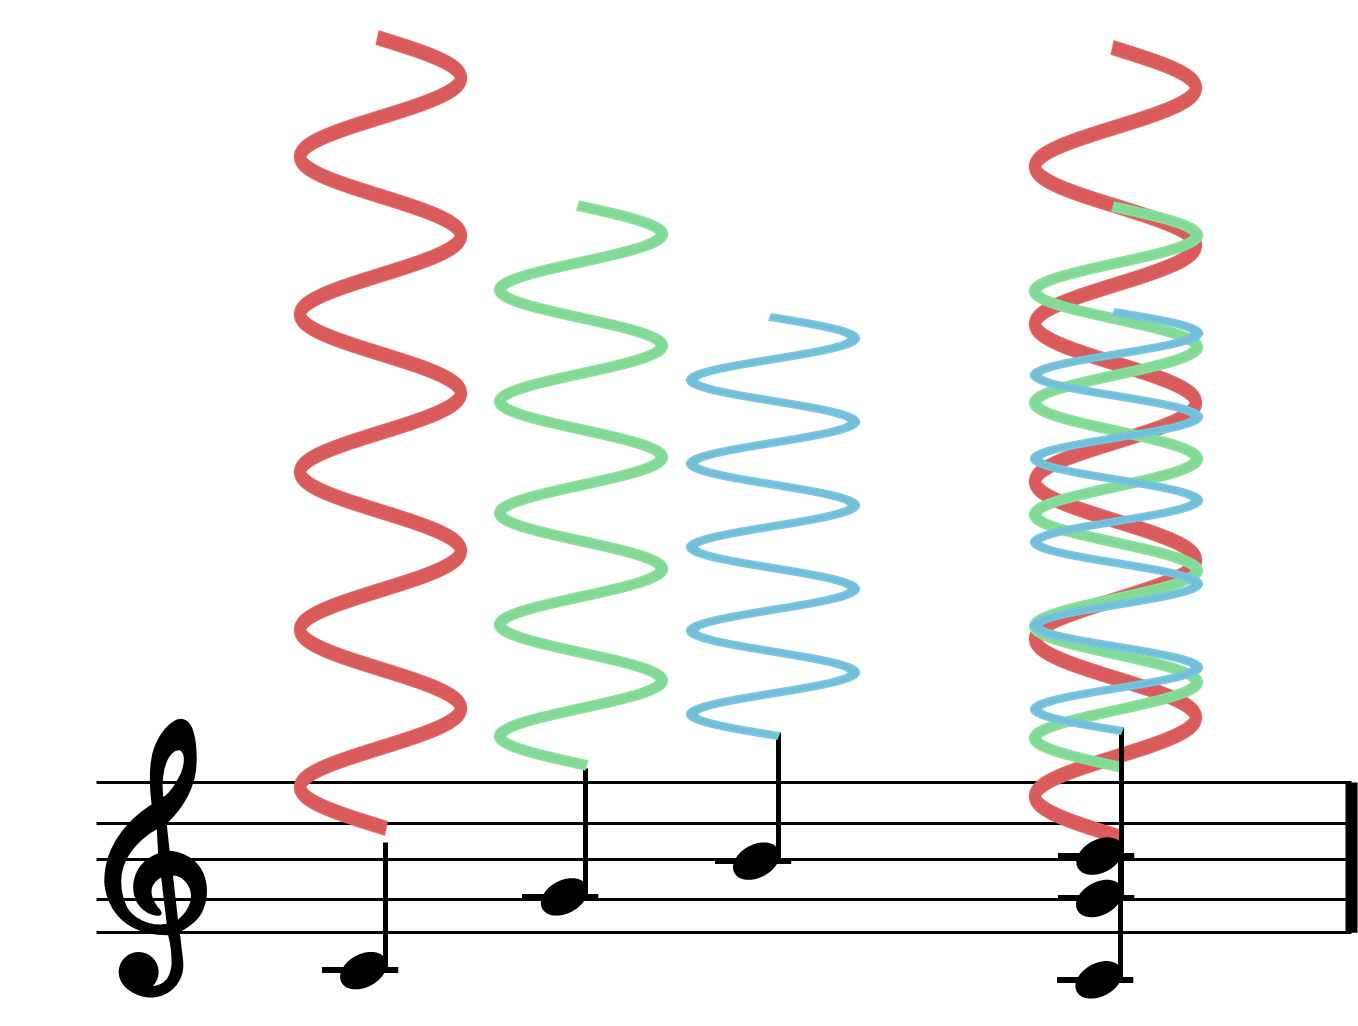
\includegraphics[width=0.7\linewidth]{Figures/tones.png}
    \caption{Illustration of random vibrations: A sum of single tones builds a resonant chord.}
    \label{fig:chords}
\end{figure}

\section{Background}
The work presented in this thesis was carried out in collaboration with Combitech AB, a Swedish consulting company within the defense, security, and industrial sectors. Within these domains, structures with bolted joints are commonly subjected to random vibration testing according to standards such as the NASA-STD-7001B and MIL-STD-810G before being approved for service. During the design phase, \ac{FEA} simulations must therefore predict whether the structure will survive these vibration environments. From this point on, the NASA-STD-7001B Workmanship profile is referred to as \textit{NASA}, and the MIL-STD-810G T43A profile as \textit{T43A}.

In industrial practice, engineers frequently face the decision of how to model the bolted joints. In large assemblies with dozens or even hundreds of bolts, modeling every single bolt with three-dimensional threads becomes extremely expensive. Simplified approaches are therefore necessary, but the question of which simplification is acceptable for a given application lacks a systematic answer. Existing guidelines, such as the VDI 2230 \cite{VDI} and the Sandia Bolted Joint Guideline SAND2008-0371 \cite{Sandia}, provide analytical frameworks for bolt design but do not directly address the trade-off between accuracy and cost in \ac{FEA} modeling. This thesis aims to fill that gap by providing guidelines based on measurable physical phenomena and a quantitative efficiency ratio for fatigue failure.

\section{Problem Statement} \label{sec:problemStatement}
This thesis aims to develop guidelines for resource-efficient Finite Element Analysis of bolted joints. To achieve this, the work focuses on one central research question:
\begin{quote}
    \textit{\RQ}    
\end{quote}

The thesis will test the following hypothesis:

\begin{quote}
    \textit{\HYP}    
\end{quote}

To support the main research question, the study considers three sub-questions:
\begin{enumerate}
    \item Which physical phenomena under random vibration that contribute to fatigue require a high-fidelity bolt representation?
    \item For which response quantities are simplified bolt models sufficiently accurate?
    \item How should computational cost and predictive accuracy be compared in a practical engineering workflow?
\end{enumerate}

Sub-questions 1 and 2 are addressed through the phenomenon-method matrix (Table \ref{tab:phenomenaMethodMatrix}), which maps physical phenomena and response quantities to the minimum modeling fidelity required to capture them. Sub-question 3 is addressed through the cost-normalized efficiency ratio defined in Section \ref{sec:Deliverables} and reported per case in Section \ref{sec:EfficiencyMetric}. Together, these form the engineering workflow referred to in the research question.

In this thesis, \textit{cost} refers strictly to the computational cost of the \ac{FE} simulation itself. Preprocessing and meshing are excluded. The formal cost metric and its normalization are defined in Section \ref{sec:costMetric}.
\newpage
\section{Thesis objectives}

% A famous quote from statistician George Box, \textit{"all models are wrong, but some are useful"}.

The thesis aims to provide a matrix of phenomena observed in bolted joints under random vibration excitation, explaining which \ac{FE} modeling method is required and which analysis is needed. The thesis will also aim to derive a quantitative measure of the computational efficiency of bolted joints under random vibration with respect to fatigue failure. 

The objective of the thesis is to deliver engineering guidelines for computational engineers to follow when working on bolted joints subjected to random vibration.

The phenomenon-method matrix is literature-based, while the computational study is benchmark-based. The matrix maps what information each representation can provide, while the benchmarking compares how accurately the studied simplified models reproduce fatigue-related response in the present single-bolt benchmark.

\section{Limitations and Scope} \label{sec:limitations}

The field of bolted-joint analysis resembles a jungle: dense, interconnected, and full of distinct species: different bolt sizes and grades, different clamped-member materials, different excitation environments, different failure modes, and different analysis methods. A single thesis cannot survey the whole jungle. The present work clears and studies one small grove: a single M10 steel bolt joining steel plates, excited by two standardized vibration profiles, analyzed for fatigue using four \ac{FE} bolt representations. The resulting guidelines are intended to be defensible within that grove and to motivate further exploration of the surrounding terrain, not to map the jungle as a whole.

The analysis considers only random vibration loading characterized by \ac{PSD} functions and bolt pretension, with two standardized load cases following NASA-STD-7001B and MIL-STD-810G. Temperature effects are excluded, all simulations assume room-temperature conditions. This is justified because the focus is on the relative accuracy of different bolt modeling strategies, and thermo-mechanical effects would affect all modeling strategies similarly.

The excitation is applied in one direction at a time rather than as combined multi-axial loading. A simple estimate suggests this is a reasonable simplification: combining the maximum stresses observed in each direction as orthogonal contributions gives $\sqrt{7^2 + 20^2} \approx 21.18$ MPa for the NASA Workmanship (a 6 \% increase over the worst single-axis stress of $20$ MPa) and $\sqrt{2.6^2 + 60^2} \approx 60.05$ MPa for the T43A excitation (an increase of less than 1 \%). These estimates assume independent superposition and do not capture any modal cross-coupling. The errors may appear small in stress, but computing the fatigue life with a 6 \% underestimate of stress gives, in accordance with equation \ref{eq:underEstimateStress}, a 28\% overestimation of fatigue life with the SN-curve used in this thesis ($(1-0.06)^{-4} = 1.281$). Therefore, multiaxial excitation is a necessary future work.

All components were assigned the same isotropic linear-elastic material properties ($E = 200$ GPa, $\nu = 0.30$). The objective is to compare bolt modeling approaches under identical assumptions, so that differences in the results are due to the bolt representation itself, rather than from changes in the material input. The ranking should therefore be interpreted as a comparative ranking for structures made from similar metallic materials with comparable elastic properties. The calculated fatigue lives depend on the chosen SN data and are not material-independent life predictions.

The main limitation of this thesis is that the quantitative guideline is strongest only in the geometrical region where all models are comparable. In local bolt regions, the simplified methods are not only less accurate but also fail to produce comparable results, making it difficult to define a single universal efficiency metric. The proposed guidelines are intended to support, not replace, engineering judgment. The remaining scope limitations are:

\begin{enumerate}
    \item Geometric scope: a single-bolt benchmark was used (Chapter \ref{chp:method}). Multi-bolt patterns, flange joints, and lap joints are not represented, so the ranking should be revalidated on multi-bolt geometries before being applied to a production assembly.
    \item Dynamic scope: a linear perturbation frequency-domain analysis was used, with the contact state frozen at the end of the initial nonlinear static preload step. Contact-status dependent phenomena, such as macro-slip and contact opening, are therefore not represented. For excitation amplitudes high enough to drive slipping, fully nonlinear transient analysis is required, and the present ranking cannot be assumed to remain valid.
    \item Excitation scope: Only the NASA-STD-7001B Workmanship and the MIL-STD-810G T43A profiles were tested. The agreement between Dirlik and Steinberg and the spread of the Ranking Index were found to depend on the signal.
    \item Validation scope: the reference model is a 3D solid bolt without threads, not a physical test. The Ranking Index is therefore relative to a higher-fidelity model rather than the actual measured fatigue life.
\end{enumerate}

\section{Contribution}
This thesis delivers three decision aids for \ac{FEA} of bolted joints under random-vibration fatigue:
\begin{enumerate}
    \item A phenomenon-method matrix (Table \ref{tab:phenomenaMethodMatrix}) linking eight physical phenomena that bolted joints may experience under random vibration to the cheapest \ac{FE} representation capable of capturing each.
    \item A decision flowchart (Figure \ref{fig:decisionTree}) that walks an engineer from the engineering question to a recommended model type and analysis setup.
\end{enumerate}

These are supported by a comparative computational benchmark of four bolt representations in a single-bolt joint under two \ac{PSD} excitations and two loading directions, which quantifies the trade-off between computational cost and fatigue-related response accuracy. The contribution is intended to complement engineering judgment rather than to replace it: it is a scoped engineering decision aid, not a universal set of rules.

\newpage
\section{Ethical, Societal, and Sustainability Aspects}
The work in this thesis concerns engineering decisions where simplification is necessary but, in many cases, must not compromise trust in the results. 

A simplified bolt representation can save significant computational time, but it may lose effects that are critical to fatigue life. The engineer has an ethical responsibility to select the simplest model that can still answer the intended engineering question, rather than the cheapest model in general. The guidelines proposed in this thesis are not intended to justify aggressive simplification without reflection, but to make the assumptions, scope, and limits of each choice more transparent. In that sense, the phenomenon-method matrix and decision flowchart support more traceable and more defensible engineering judgment. From a societal perspective, more robust engineering workflows can improve products and shorten development time without lowering computational quality. This can support faster iteration, clearer communication between analysts and decision makers, and better prioritization of where detailed analysis is truly needed. High-fidelity finite element analysis is not only expensive in engineering time but also in computational resources. Repeated use of over-detailed models increases energy use and hardware demand. A more resource-efficient modeling strategy can therefore contribute to more sustainable engineering practice.

\section{Outline}
%\item Chapter \ref{chp:introduction} presents the limitations/ scope of the thesis, this outline, the background, the contribution, and the problem statement.
The thesis is outlined as:
\begin{itemize}
    \item Chapter \ref{chp:theory} presents the theoretical background for bolted joints, preload, stiffness models according to VDI 2230 and Sandia SAND2008-0371, vibration-related fatigue phenomena, modal and random-vibration analysis, and the frequency-domain fatigue methods used later.
    \item Chapter \ref{chp:relatedwork} reviews the related literature on bolt modeling fidelity, spectral fatigue methods, and experimental validation, and identifies the gap that this thesis addresses.
    \item Chapter \ref{chp:method} describes the comparative computational experiment, including the four modeling strategies, the loading cases, the extraction regions, the accuracy, and the cost metrics used to compare the models.
    \item Chapter \ref{chp:results} presents the results of the comparison and derives the practical guidelines.
    \item Chapter \ref{chp:discussion} discusses what the results support, their limitations, and how they relate to previous work.
    \item Chapter \ref{chp:conclusions} answers the research question, states whether the hypothesis is supported, summarises the contribution, and outlines future work.
\end{itemize}

\chapter{Theory} \label{chp:theory}
This chapter presents the theoretical background required to analyze bolted joints under random vibration. The chapter covers bolt mechanics, preload, stiffness modeling, vibration-related fatigue phenomena, fundamentals of modal analysis, random vibration, and finite element analysis. The purpose is to establish the concepts and relationships that are later used in the method, results, and discussion.


\section{Bolt Theory}
\subsection{Bolt Geometry}

The geometry of bolts is simple, but different standards use different words for the same dimension. In this thesis, the following geometry names are used:
\begin{enumerate}
    \item $d$: Nominal bolt diameter, the main shaft diameter, see Figure \ref{fig:Bolt1}.
    \item $d_1$: The minimum diameter of the threads, measured at the "valleys" of the threads, see Figure \ref{fig:Threads}.
    \item $d_2$: The pitch diameter of the threads, measured at the "peaks" of the threads, see Figure \ref{fig:Threads}.
    \item $d_3$: Minor thread-root diameter.
    \item $d_h$: Hole diameter.
    \item $d_w$: Bearing diameter of the bolt (The diameter of the surface under the bolt head or nut).
    \item $d_{wa}$: Bearing diameter of the largest area that is between the bolt, nut, or washer and the clamped members. Usually, if a washer is used, this is the washer diameter, see Figure \ref{fig:wNut}.
    \item $d_{w, eff}$: Effective bearing diameter used in the analytical stiffness models. For the joint analysed here, $d_w = 15$ mm, $d_{wa} = 20$ mm, and $d_{w,eff} = 17.56$ mm.
    \item $A_s$: The Tensile stress area of the bolt, the effective cross-sectional area of the threaded section that resists tensile loading, which is less than the nominal area of the shank, see Figure \ref{fig:Bolt1}. 
\end{enumerate}

\begin{figure}[H]
    \centering
    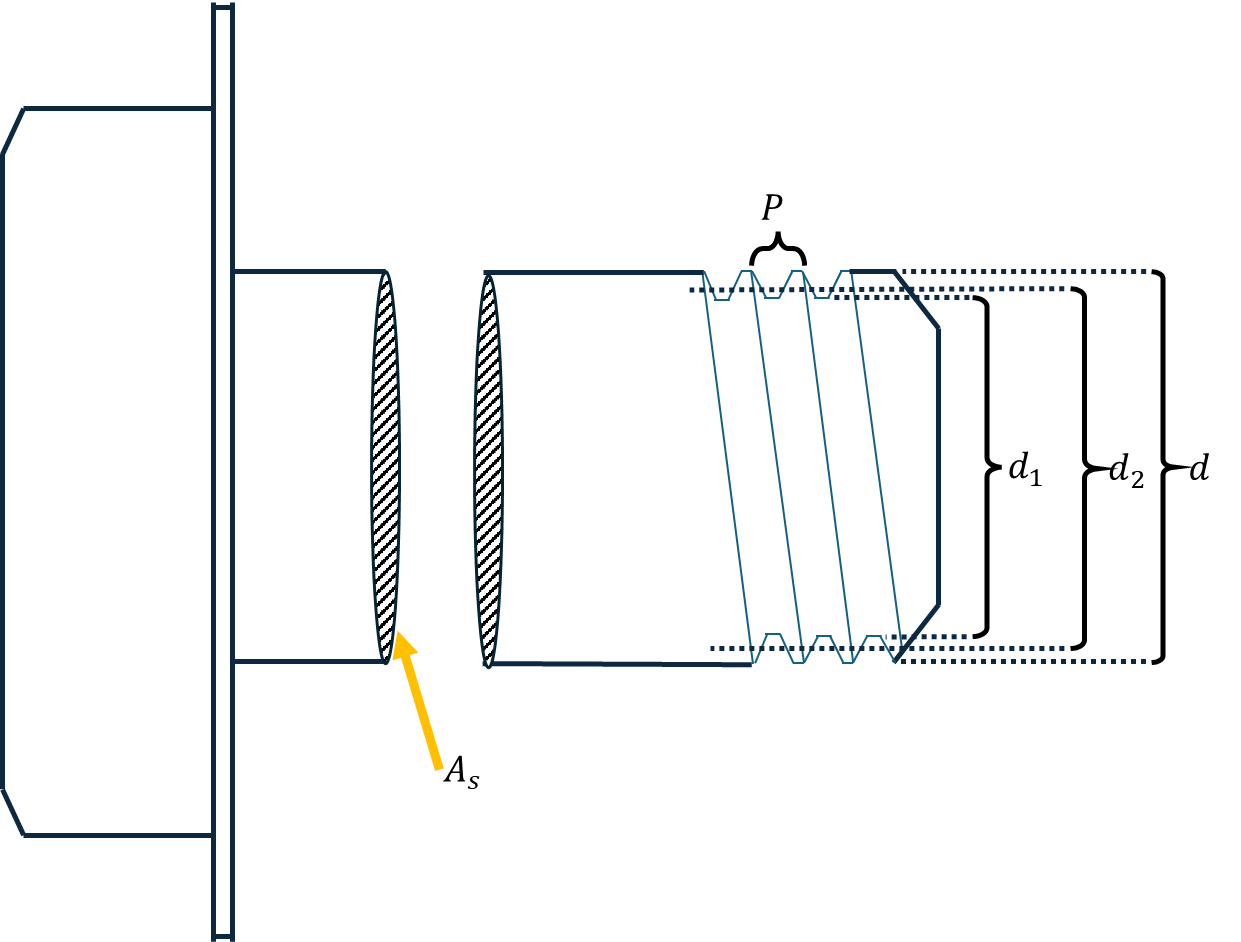
\includegraphics[width=0.75\linewidth]{Figures/boltGeometry1.png}
    \caption{Geometry of a bolt.}
    \label{fig:Bolt1}
\end{figure}

\begin{figure}[H]
    \centering
    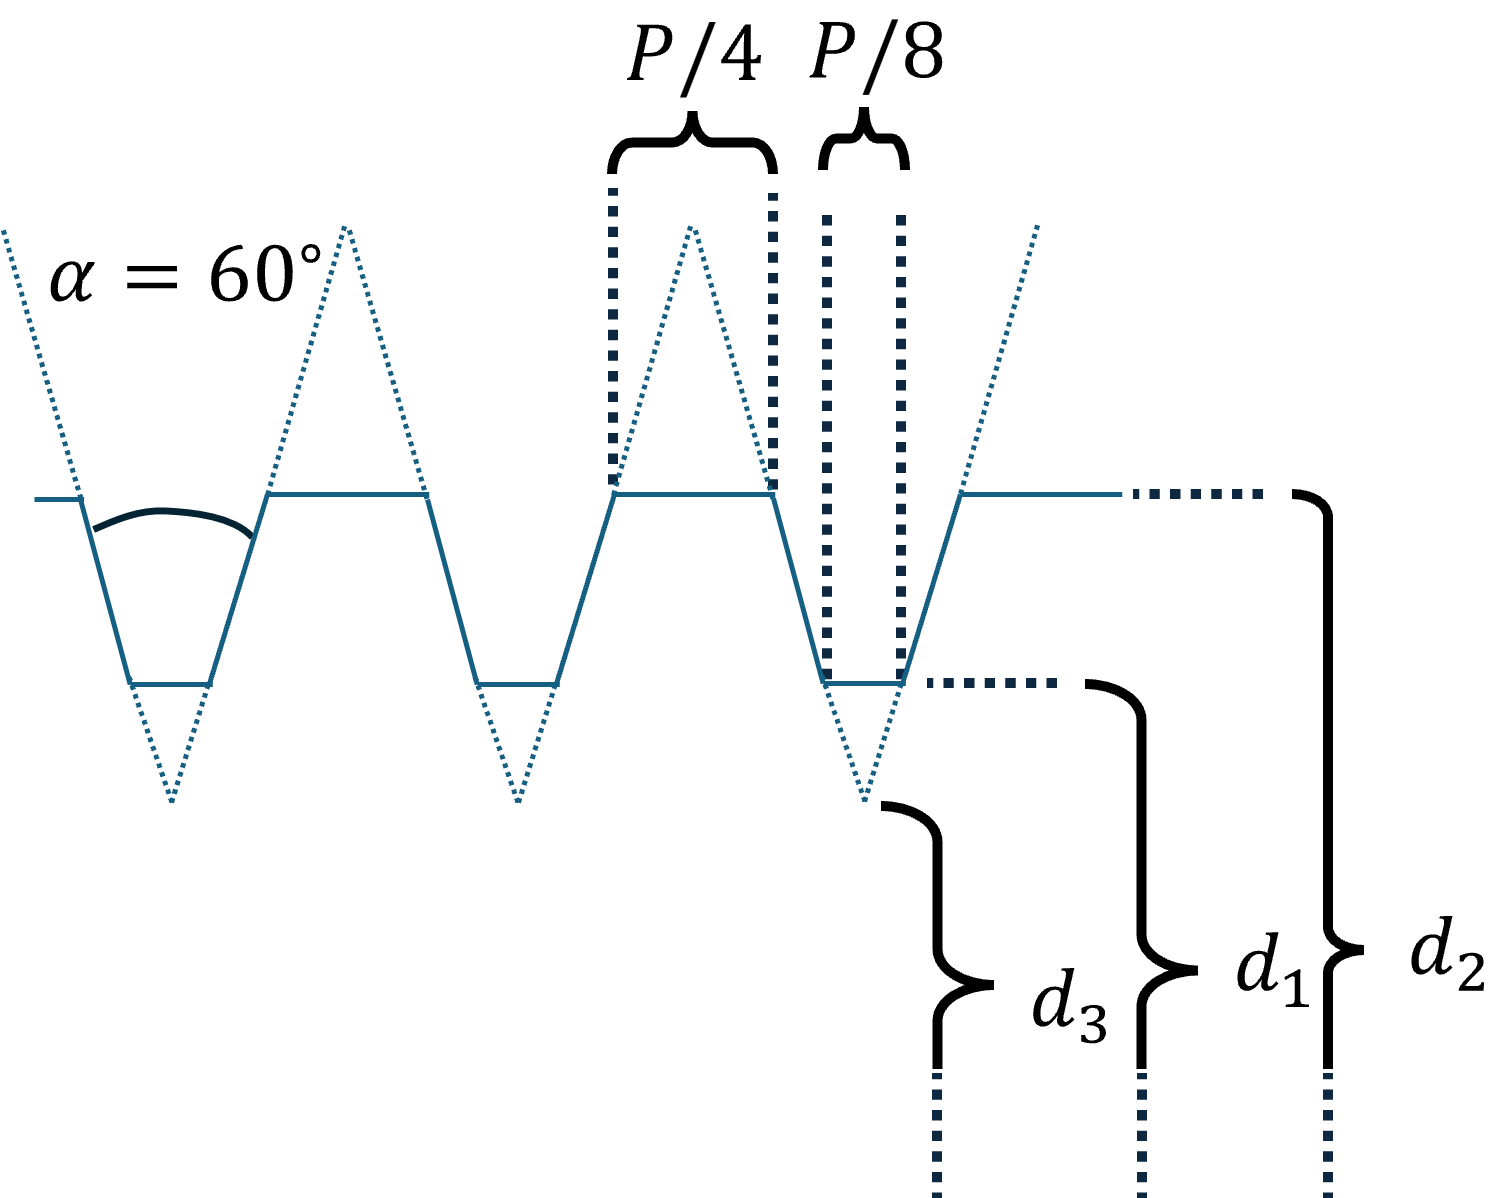
\includegraphics[width=0.75\linewidth]{Figures/threadGeometry.png}
    \caption{The most important dimensions of threads.}
    \label{fig:Threads}
\end{figure}

The equation to compute the tensile stress area is found in handbooks on bolted joints and also in SS-EN-ISO898-1-2013 \cite{SSENISO898-1-2013}:

\begin{equation} \label{eq:TensileStressArea}
    A_s = \frac{\pi}{4} \left( \frac{d_2 + d_3}{2} \right)^2
\end{equation}

\begin{figure}[H]
    \centering
    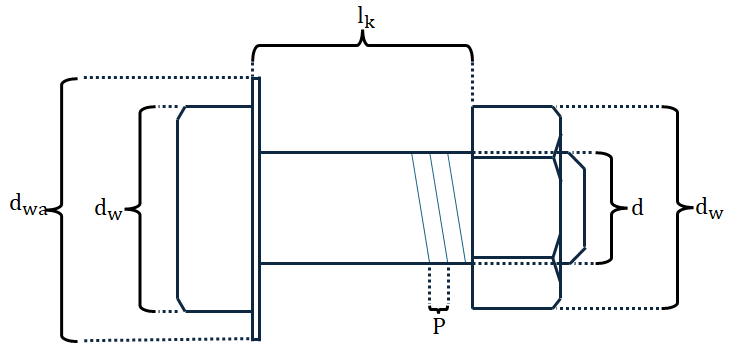
\includegraphics[width=0.75\linewidth]{Figures/geometryWNut.png}
    \caption{The most important dimensions of a bolt with a nut.}
    \label{fig:wNut}
\end{figure}

\subsection{Preload} % 
The preload, or pretension, is the tensile force $F_M$ in the bolt that sets the clamp force on the members. It is what makes the bolted joint so strong - it's the main force creating friction that takes care of shear loads on the structure and the reason why a bolt itself only experiences a fraction of a total axial load. Typically, the preload is specified as a fraction of yield or ultimate tensile stress. The VDI 2230 standard recommends using 90 percent of the bolt's yield strength \cite{VDI}, but common practice is between 70 and 90 percent. For joints subjected to cyclic loading and for joints using bolts of high-strength materials, the MIL-HDBK-60 recommends a maximum preload of 75 - 90 \% of yield strength \cite{MIL-HDBK-60}. One intuitive way of explaining the importance of preload is a bolt diagram, as seen in Figure \ref{fig:Joint Diagram}:

\begin{figure}[H]
    \centering
    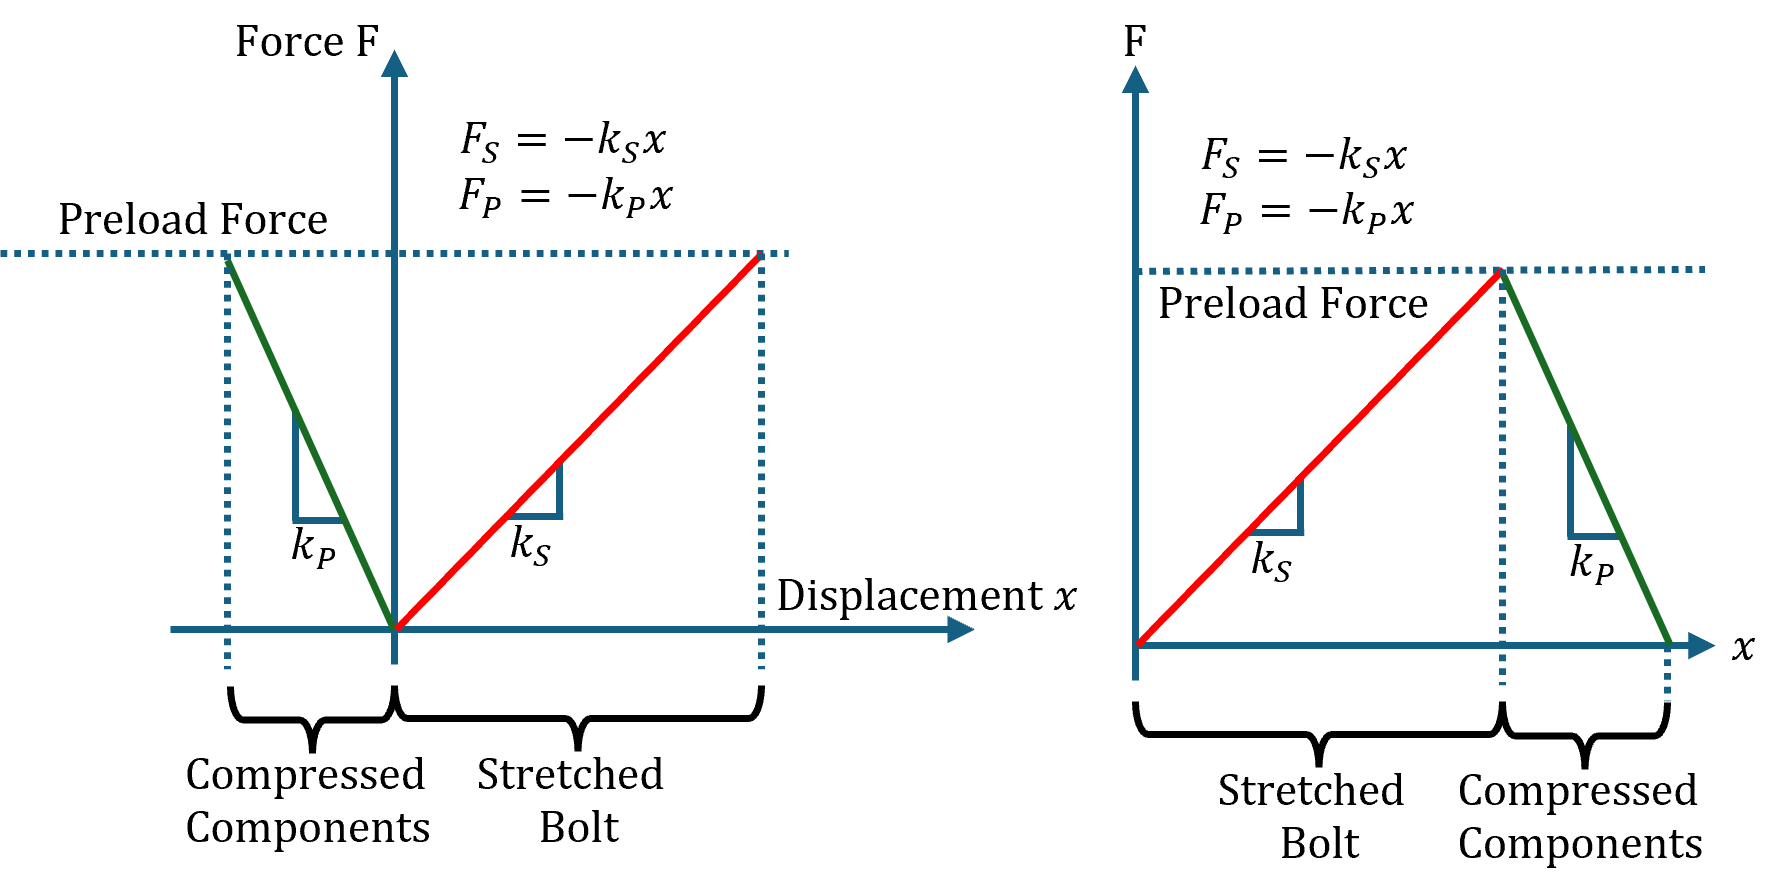
\includegraphics[width=1\linewidth]{Figures/Bolt Diagrams.png}
    \caption{Bolt (joint) diagram for a preloaded joint. The bolt-force line and the member-force line are plotted against deformation. Their intersection sets the preload $F_M$, which fixes the bolt elongation and the member compression at assembly. Left: the two lines plotted from a common origin. Right: the member line has been shifted to begin at the end of the bolt line, making the load sharing easier to read.}
    \label{fig:Joint Diagram}
\end{figure}

When a preload is applied, it causes the bolt to stretch (positive displacement) and the clamped members to compress (negative compression), as seen in the left diagram in Figure \ref{fig:Joint Diagram}. It is common to move the plot of the compressed members to be directly after the plot for the stretched bolt since it makes visualizing easier (the right diagram in Figure \ref{fig:Joint Diagram}).

When an external tensile load $F_L$ is applied to the joint, the bolt stretch increases (change of bolt force $\Delta F_S$), while the members' compression decreases (change of member force $\Delta F_P$). Since the members are (preferably) much stiffer than the bolt, the reduced clamping absorbs most of the applied load. This is seen in the left diagram in Figure \ref{fig:Joint Diagrams Loaded}:

\begin{figure}[H]
    \centering
    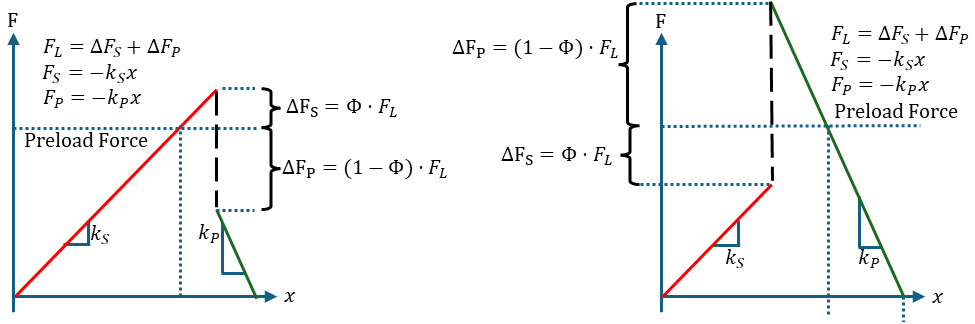
\includegraphics[width=1\linewidth]{Figures/Bolt Diagrams Loaded.png}
    \caption{Joint Diagrams Loaded}
    \label{fig:Joint Diagrams Loaded}
\end{figure}

If an external compressional load $F_L$ pushes the members closer together, the bolt stretch decreases and the members' compression increases. Still, the member's compression takes the hit, but another problem arises - if the bolt force (displacement) becomes zero, it's no longer tightened and might loosen \cite{Colly}. This is visualized in the right diagram in Figure \ref{fig:Joint Diagrams Loaded}. The quantitative load-sharing relationship is given by the preload
efficiency factor $\Phi$ in Equation \ref{eq:PreloadFactor}, and is dependent on the bolt stiffness $k_S$ and clamped-member stiffness $k_m$.

\newpage
\subsection{Analytical Standard VDI 2230} \label{sec:VDI}
The VDI 2230 standard provides an analytical method for bolted-joint design. It models clamped-member compliance with an equivalent cone, distributes applied torque among bearing friction, thread friction, and useful preload, and captures load sharing through the preload efficiency factor $\Phi$. In this thesis, VDI 2230 is used as an analytical reference for bolt compliance, clamped-member compliance, and the load-sharing factor $\Phi$. The complete set of formulas used in this thesis, including the cone angle $\varphi$, the substitution cylinder, the member compliance $\delta_P$, and the torque distribution, is reproduced in Appendix \ref{app:bolt_derivations}, Section \ref{sec:VDIApp}.

\subsection{Sandia National Laboratories SAND2008-0371}
The Sandia National Laboratories SAND2008-0371 \textit{Guideline for Bolted Joint Design and Analysis: Version 1.0} includes several methods for computing bolted joint stiffness \cite{Sandia}. One of these is Shigley's frustum approach, which is very similar to the VDI 2230. There is the Cylindrical Stress Field Method (Q Factor), and, lastly, the empirical method recommended by the Sandia report.

\subsubsection{Q-factor} \label{sec:QFactor}
The simplest Sandia method assumes that the stress field is distributed as a cylinder of diameter $D_c$. A factor $q_i$ is defined as the ratio between the hole diameter $d_h$ and the bolt diameter $d$, taking clearance into account. The factor $Q$ can be defined in different ways. This is described in more detail in Appendix \ref{app:QFactor}.
\begin{figure}[H]
    \centering
    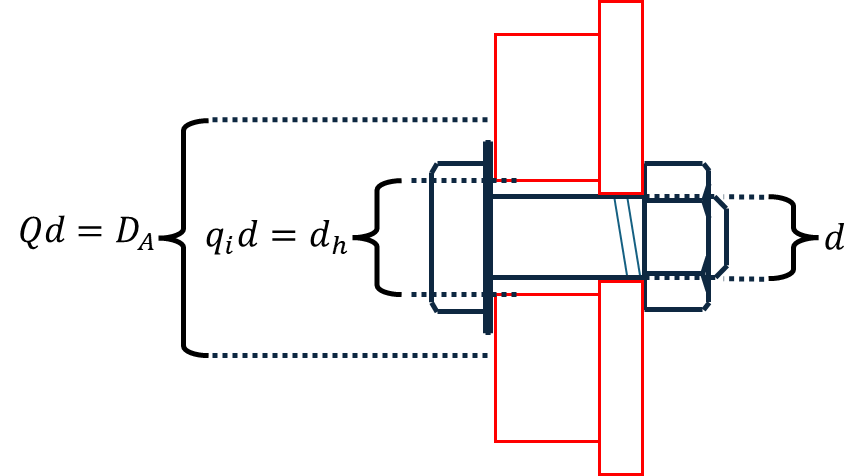
\includegraphics[width=0.8\linewidth]{Figures/SandiaDimensions.png}
    \caption{Dimensions used in the Q-factor approach to formulate bolted joint stiffness.}
    \label{fig:QFactorDimensions}
\end{figure}


\newpage
\subsubsection{Sandia DMP Empirical Method} \label{sec:DMP}
Another method that is described in the Sandia report is the \ac{DMP} formulation. The member stiffness $k_m$ for a two-layer joint is written as in Equation \ref{eq:DMB_Member1} - \ref{eq:DMB_Member4}:
\begin{equation} \label{eq:DMB_Member1}
    E_{eff} = (E_{max}^{-1} + n\cdot(E_{min}^{-1} - E_{max}^{-1}))^{-1}
\end{equation}
\begin{equation} \label{eq:DMB_Member2}
    N_k = 0.9991 x_G + 0.2189n + 0.5234
\end{equation}
\begin{equation} \label{eq:DMB_Member3}
    x_G = \frac{d_b}{l_k}\left[\frac{d_h^2 - d_c^2}{1.25 d_b^2} \right]
\end{equation}
\begin{equation}\label{eq:DMB_Member4}
    k_m = E_{eff} d_b N_k,
\end{equation}

where:
\begin{itemize}
    \item $n = \tfrac{l_{ls}}{l_k}$ is the ratio of "less stiff" (subscript ls) material length divided by the total clamping length.
    \item $E_{max}$ and $E_{min}$ are the largest and smallest Young's moduli of the materials.
    \item $x_G$ is a factor dependent on bolt diameter, hole diameter, clamp length, and head diameter.
    \item $N_k$ is a non-dimensional stiffness representation.
\end{itemize}

According to the standard, the DMP method is valid only if $\tfrac{d}{l_k} \in [0.167; 1.786]$ and has a standard error of 0.065 in the curve-fitting relative to the FE-based dimensionless stiffness data $N_k = \tfrac{k_m}{E_{eff}d}$ it was generated with (it is not a percentage error in $k_m$ or as against experimental measurements). The Sandia report recommends using the DMP method when the validity condition is met and falling back to the frustum approach when it is not.

\subsection{Axial- and Bending Stiffness}
A bolt resists both axial, bending, and torsional loads. Therefore, it has stiffness in these three directions.

To compute the bending stiffness, the second moment of area (also called the area moment of inertia) must be determined. For circular shapes such as a bolt shank, it is defined by Equation \ref{eq:moment_Area}:
\begin{equation} \label{eq:moment_Area}
    I = \frac{\pi}{64} d^4.
\end{equation}

The moment of area is then used to compute the bending stiffness:

\begin{equation}
    k_{bend} = \frac{EI}{L}.
\end{equation}

For both the VDI cone model and the Sandia methods, this is performed for each bolt section (Figure \ref{fig:Bolt_Nut_Young_compl}), and the results are then summed. The only difference is the definition of $d^4$ in the Q-factor, see Appendix \ref{app:bolt_derivations}.

\begin{equation}
    \delta_{bend} = \sum_i \frac{L_i}{E_i I_i},
\end{equation}
\begin{equation}
    k_{bend} = \delta_{bend}^{-1}
\end{equation}
where $I_i$ is evaluated by Equation \ref{eq:I_VDI} for the VDI 2230 approach Equation \ref{eq:Sandia_moment_inertia} for the Sandia approach.

The bending stiffness per layer follows from $k_{bend, i} = E_iI_i/L_i$, and combining these layers in series yields the total bending stiffness. The Sandia report warns that this approach may be non-conservative.


\begin{equation} \label{eq:I_VDI}
    I_i = \frac{\pi}{64} d_i^4
\end{equation}

\begin{equation} \label{eq:Sandia_moment_inertia}
    I_i = \frac{\pi}{64} \left[ (Qd)^4 - (q_id)^4 \right] = \frac{\pi d^4 (Q^4 - q_i^4)}{64}
\end{equation}

\subsection{Shear Stiffness from Timoshenko Beam Theory and Torsional Stiffness from Saint-Venant torsion}
Neither the VDI 2230 nor the Sandia report addresses shear or torsional stiffness.

The Timoshenko beam theory accounts for shear. Its shear stiffness derivation is reproduced in Appendix \ref{app:bolt_derivations}, Section \ref{sec:Timoshenko}. The theory is intended for slender beams, typically with a slenderness ratio $\tfrac{l_k}{d}$ above 5-10. Below this range, the shear coefficient $\kappa$ becomes geometry-sensitive, and full 3D elasticity is more appropriate. For the M10 bolt in this thesis, the slenderness ratio is $\tfrac{8.46\cdot 2 + 1.6}{10} = 1.8$ (Figure \ref{fig:Drawing1}), well below the valid limit. Therefore, the Timoshenko beam theory is not valid here, but is used as an analytical estimate for the shear stiffness in the CBUSH bolt representation (a six-degree-of-freedom spring element, introduced in Section \ref{sec:FEA}).

The Saint-Venant theory accounts for torsion. Its torsion stiffness is reproduced in Appendix \ref{app:bolt_derivations}, Section \ref{sec:SaintVenant}. The theory assumes a bar in pure uniform torsion with unrestrained end warping. For a circular bolt shank loaded only by tightening torque, this is reasonable since the cross-section can warp freely and the shank is approximately a bar between the head and threads. 

\subsection{Preload Efficiency Factor}
One important concept in bolted joints is the preload efficiency factor $\Phi$, which describes how external loads are distributed between the bolt and clamped components \cite{VDI}, \cite{Sandia}. In both Sandia and VDI 2230, it is defined as per Equation \ref{eq:PreloadFactor}:

\begin{equation} \label{eq:PreloadFactor}
    \Phi = \frac{k_S}{k_S+k_m} = \frac{\delta_P}{\delta_S + \delta_P}.
\end{equation}
This dimensionless factor indicates that when an external tensile load is applied to a preloaded joint, the load is shared between the bolt and the clamped components in proportion to their relative stiffnesses, provided the joint remains closed. The factor is used to find the bolt load due to an external load $F_e$ by multiplying the Preload Efficiency Factor by the external load as in Equation \ref{eq:deltaFs}:
\begin{equation} \label{eq:deltaFs}
    \Delta F_S = \Phi \cdot F_e    
\end{equation}

This is especially important when working with fatigue, since the alternating stress range experienced by the bolt is only $\Phi$ times the alternating external load. A stiffer joint (a higher $k_m$ relative to $k_S$) results in a smaller preload efficiency factor, and less of the external load is transferred to the bolt. A very compliant joint (low $k_m$ relative to $k_S$) gives a higher $\Phi$-value, and more of the external load directly stresses the bolt. This is also addressed and confirmed by Okorn \cite{30}.


\section{Fatigue phenomena for bolted joints under vibration} \label{sec:fatiguePhenomena}
When a bolted joint is subjected to vibration, several interacting physical phenomena affect it. Understanding these phenomena is necessary to determine whether each is worth modeling in \ac{FEA},  since each imposes different demands on model fidelity and required analysis. 

For each phenomenon, four questions are useful: \textit{1) What is the phenomenon?}, \textit{2) What does the phenomenon cause?}, \textit{3) How can it be modeled in \ac{FEA}?}, and \textit{4) when can it be handled analytically rather than in \ac{FEA}?}.

The capability of the four FE-modeling methods in this thesis (bonded, CBUSH, beam, threadless solid), together with the fully threaded solid, to capture each phenomenon is summarised in the phenomenon-method matrix in Table \ref{tab:phenomenaMethodMatrix}.

The eight phenomena are presented in an order that reflects their causal tendencies. First is slipping, because it acts as a gatekeeper for several other phenomena. Second are slip-dependent phenomena such as stage-2 self-loosening and hole elongation. Third is independent mechanisms such as embedding, bolt bending, torsion, and stress concentration. Last is the final cumulative outcome, fatigue failure.

\subsection{Slipping}
Slipping in a bolted joint happens when a transverse (shear) load exceeds the friction force holding the clamped plates together \cite{49}. That friction limit is given by Equation \ref{eq:Friction}:

\begin{equation} \label{eq:Friction}
    F_{Friction} = F_M\times \mu,
\end{equation}

where $F_M$ is preload and $\mu$ is friction coefficient between the clamped members. Slipping occurs when $F_{shear} \ge F_M\mu$. Three combinations of parameters can drive the joint across the slip condition:
\begin{enumerate}
    \item Insufficient preload.
    \item Low friction coefficient $\mu$, typically from smooth or lubricated surfaces.
    \item High transverse load $F_{shear}$.
\end{enumerate}

Once slipping starts, the bolt may begin to bear against the hole wall, adding shear and bending stresses to the bolt. Repeated micro-slips can accumulate into nut rotation (stage-2 self-loosening). The rubbing interface can develop fretting wear.

Slipping can be captured in \ac{FEA} using surface-to-surface frictional contacts between the clamped members. The key requirement is that the contact pressure distribution (normal force) and the friction coefficient are correctly represented where slipping may occur. Slip modeling is largely independent of how the bolt is represented, as long as the model correctly transfers the clamping force to the clamped parts. Modeling the bolt as a surface bond is not appropriate, as it removes friction entirely and eliminates the slip degree of freedom.

When only a binary answer is needed, whether the joint can slip at all, the slip condition can be evaluated analytically without \ac{FEA} using the nominal shear load, preload, and a tabulated friction coefficient.

\subsection{Self-Loosening}
Jiang \textit{et al.} describe self-loosening as a two-stage process \cite{58}. In \textit{stage 1}, the clamping force drops without nut-bolt rotation, driven by other mechanisms such as embedding at the contact surfaces or between threads. In \textit{stage 2}, the nut rotates relative to the bolt. Small angular displacements per vibration cycle accumulate to a significant amount over thousands of cycles.

Both stages reduce the bolt's preload. Since preload clamps the joint and resists opening or slipping, lower preload increases cyclic stress in the bolt and reduces friction between the parts, which together accelerate fatigue failure.

The two stages have different modeling requirements. Stage 1 can be treated as a preload reduction: the preload is reduced analytically (see Embedding, Section \ref{sec:embedding}) before the simulation is run. Stage 2 requires nonlinear transient analysis with frictional contacts between the threads, the nut bearing surface, and the clamped members \cite{siemens_bolt_analysis_2026}. Only the fully threaded 3D solid with frictional contacts can simulate stage 2, and the analysis must be performed in the time domain, since the frequency-domain random-vibration analysis used in this thesis assumes linear behavior. Zhang \textit{et al.} used ABAQUS infinitesimal-sliding contact at the threads and confirmed that a full 3D thread model is necessary to capture stage-2 rotation \cite{52}.

Stage 2 self-loosening is conditional on slipping: if the slip condition (Equation \ref{eq:Friction}) is not met, stage 2 cannot occur. Stage 1 is independent of slip and can occur even in a non-slipping joint.

\subsection{Hole Elongation}
Hole elongation is a permanent deformation of the bolt hole in the clamped members, caused by bearing contact between the bolt shank and the hole wall. It occurs after the joint has slipped and the bolt has been driven against the hole.

Hole elongation changes the effective clearance and introduces additional stress concentrations at the hole edge, which can initiate fatigue cracks. In multi-bolt configurations, it also redistributes load between fasteners. Under random vibration, progressive hole elongation increases the relative motion available at the joint, which can in turn promote further slipping.

Capturing hole elongation in \ac{FEA} requires contact between the bolt shank and the hole wall, combined with an elasto-plastic material model for the clamped members. Only the solid models have a physical shank that can bear against the hole. 

Hole elongation requires both slip and a bearing stress high enough to yield the hole material. The slip condition is therefore a necessary but not sufficient condition for hole elongation. The bearing stress can be estimated analytically using Equation \ref{eq:hole-elong}:

\begin{equation} \label{eq:hole-elong}
    \sigma_{bearing} = \frac{F_{shear}}{d_{bolt} \cdot t},
\end{equation}

where $d_{bolt}$ is the bolt-shank diameter and $t$ is the thickness of the thinnest (or weakest) clamped plate. Comparing $\sigma_{bearing}$ with the yield strength of the plate material gives an indicator of whether hole elongation can occur.

\subsection{Embedding} \label{sec:embedding}
Embedding is a small-scale plastic deformation that smooths the microscopic surface roughness of the contact surfaces between the bolt head, nut, clamped members, and threads. It occurs mainly during initial tightening and in the early service life, as high pressure flattens irregularities in the surface finishes \cite{VDI}, \cite{Colly}.

\begin{figure}[H]
    \centering
    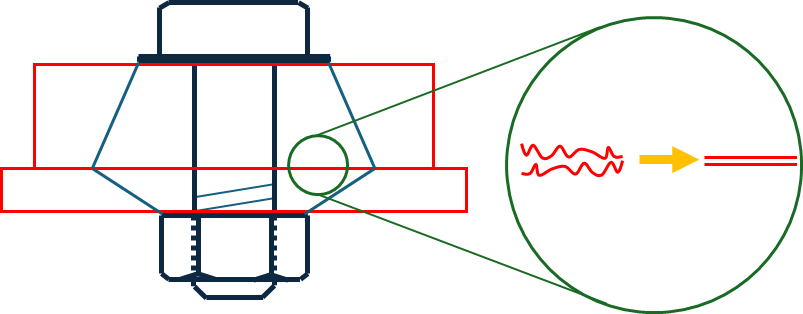
\includegraphics[width=0.5\linewidth]{Figures/Embedding.png}
    \caption{The embedding process. Compression in the clamped members (and bolt) smooths microscopic surface irregularities, reducing the total grip length.}
    \label{fig:Embedding}
\end{figure}

Under vibration loading, embedding can develop earlier than under static conditions. The resulting preload loss reduces joint stiffness and increases the alternating stress on the bolt, shortening fatigue life. According to \textit{Handbok om Skruvförband} (Colly Components AB) and VDI 2230, a joint's ability to handle embedding scales with the slenderness ratio $\tfrac{l_k}{d}$: a more slender bolt tolerates embedding better because the same amount of surface deformation represents a smaller fraction of the total bolt elongation \cite{VDI}, \cite{Colly}.

Embedding permanently shortens the total grip length, producing a loss of preload $F_Z$. VDI 2230 and the Colly Handbook quantify this using the bolt diagram in Figure \ref{fig:Embedding_Diagram}, where the change in length $f_Z$ due to embedding translates into a force loss according to Equation \ref{eq:Preload_loss_embedding}:

\begin{equation} \label{eq:Preload_loss_embedding}
    F_Z = \frac{f_Z}{\delta_S + \delta_P},
\end{equation}

where $\delta_S$ is the bolt compliance and $\delta_P$ is the clamped part compliance.

\begin{figure}[H]
    \centering
    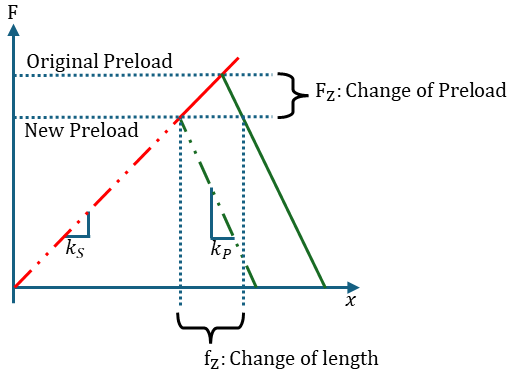
\includegraphics[width=0.5\linewidth]{Figures/Embedding_BoltDiagram.png}
    \caption{Bolt diagram visualizing the effect of embedding in a bolted joint.}
    \label{fig:Embedding_Diagram}
\end{figure}

From an \ac{FEA} perspective, embedding is straightforward in principle but expensive in practice, because a fine mesh and an elasto-plastic material model are required to capture these small deformations. A more economical approach is to compute $F_Z$ analytically using Equation \ref{eq:Preload_loss_embedding} and reduce the applied preload by this amount before running the simulations.


\subsection{Bolt bending}
Bolt bending occurs when a bolt is subjected to a moment, placing one side in tension and the opposite side in compression. In bolted joints, bending can occur from several sources, including misalignment of the clamped surfaces, loads that do not pass strictly through the bolt axis, and transverse vibrations. Under random vibration, bending moments are generated whenever the mode shapes involve rotational motion at the joint. 

Bending stresses increase the peak stress at the most loaded thread, reducing fatigue life. Bending is naturally captured by any \ac{FEA} model that contains bolt geometry. The bonded representation has no bolt geometry, so bending stress cannot be read directly from bolt-body stress. An approximate bending moment can instead be provided by using the interface grid forces at the bonded surfaces with Equation \ref{eq:bendingStress}:

\begin{equation} \label{eq:bendingStress}
    \sigma_{bend} = \frac{M}{W},
\end{equation}
where $W = \pi d_s^3 \cdot \tfrac{1}{32}$ is the elastic section modulus of the bolt shank and $d_s$ is the shank diameter \cite{budynas_shigleys_2015}. Comparing $\sigma_{bend}$ with the preload stress $\sigma_z = \tfrac{F_M}{A_S}$ indicates whether or not bending is a significant contribution to the bolt stress state.

\subsection{Torsion in the Bolt}
Torsional stress in the bolt is primarily a consequence of tightening. When a torque is applied to the nut and bolt head, only a portion of the torque is converted to axial preload, while the remainder results in residual torsional stress in the bolt shank. According to the VDI 2230, approximately 50 \% of the applied torque is consumed by bearing-surface friction under the head, around 40 \% by thread friction, and only about 10 \% generates the desired axial preload \cite{VDI}.

Residual torsion adds a shear component to the bolt stress state, which raises the equivalent (von Mises) stress, reducing the margin to fatigue failure and potentially contributing to self-loosening.

In \ac{FEA},  torsion is captured only when threaded geometry is modeled with frictional contacts and a rotational displacement or torque applied to the nut. The bolt representations and analyses used in this thesis apply preload as a direct axial force and therefore do not capture residual torsion. It can, however, be estimated analytically in post-processing using Equation \ref{eq:torsionStress}:
\begin{equation} \label{eq:torsionStress}
    \tau_M = \frac{M_G}{W_P},
\end{equation}
where $M_G$ is the thread torque ( approximately 40\% of the applied torque) and $W_P$ is the polar section modulus of the bolt shank according to Shoberg \cite{VDI_Fundamentals}. Residual torsion can therefore be added to the \ac{FEA} stress result analytically when needed.

\subsection{Stress Concentration}
Stress concentrations occur where the local geometry abruptly changes the load path, causing local stresses much higher than the nominal stress. In bolted joints, this happens at the transition between the bolt head and shank, and at the threads. The nominal stress is the stress computed from a simplified or averaged cross-sectional load assumption, whereas the local stress is the actual geometric stress peak.

According to Okorn \textit{et al.}, stress concentration factors at the thread root can reach 4-5 times the nominal stress \cite{30}.

A simplified model may reproduce the global force distribution correctly, but still fail to capture the local stress concentration responsible for crack initiation.

Stress concentrations indicate where fatigue cracks are likely to initiate. Fatigue life decreases rapidly as stress amplitude increases (as shown on the S-N curve), so even a moderate \ac{SCF} can substantially reduce the predicted life. It must therefore be included in fatigue analysis.

Capturing stress concentrations in \ac{FEA} requires solid models in regions with stress peaks. Therefore, the solid model without threads can partially capture these concentrations, whereas a solid model with threads can capture stress concentrations at the threads. It could, however, be estimated using post-process calculations, as described in Section \ref{sec:SCF} and \ref{sec:validity}, by multiplying the nominal stress by an \ac{SCF}. Stress concentration effects can sometimes be estimated analytically in post-processing, but direct \ac{FEA} capture requires solid modeling of the relevant geometric details and a fine mesh.

\newpage
\subsection{Fatigue failure}
Fatigue failure is the progressive structural damage caused by cyclic loading. The phenomena described above all contribute to fatigue failure, but are just a few examples. Fatigue failure is the final way the joint can break. When a crack initiates and grows to a certain size, the bolt can no longer carry the load.

To capture fatigue failure in \ac{FEA},  a combination of stress-life (SN-curve) analysis, cumulative damage theory, and detailed \ac{FE} modeling is typically employed. This enables the prediction of fatigue cracks in both the bolt and the clamped members under various loading conditions. A static or dynamic \ac{FEA} is first performed to determine the stress distribution throughout the joint, including regions of high stress concentration. This typically requires refined meshes around critical features such as threads and contact interfaces.


For random vibration loading, frequency-domain methods based on the stress \ac{PSD} tensor can be used. A stress-\ac{PSD} does not directly provide a cycle count. Instead, the stress \ac{PSD} is first used to compute spectral moments and statistics of the random process. These are then used to estimate an expected stress-range distribution, which is finally combined with an SN-curve and, often, with Miner's rule, to estimate fatigue life without requiring complete time histories. The Steinberg and the Dirlik frequency-domain models used in this thesis are examples of random vibration analysis \cite{dirlik_application_1985}.

The most cost-effective way to avoid fatigue failure is to design the joint so that slipping won't occur. It would eliminate many phenomena that would contribute to fatigue failure. When slip is prevented, the bolt stress state is dominated by axial preload plus elastic bending. Both are well captured by linear perturbation analysis in the frequency domain. This observation motivates the phenomenon-method matrix and decision flowchart presented in Section \ref{sec:Deliverables}.
\newpage
\section{Modal analysis}
Modal analysis decomposes the dynamic response of a structure into a set of independent modes, each characterized by a natural frequency $f_n$, a mode shape $\varphi_n$, and a modal damping ratio $\zeta_n$. For an undamped system, Equation \ref{eq:modalEigen} can be used to extract the natural frequencies (eigenvalues) and mode shapes (eigenvectors) \cite{33}. 

\begin{equation} \label{eq:modalEigen}
    [K]\varphi_n = \omega^2_n[M]\varphi_n,
\end{equation}

where $[K]$ is the stiffness matrix, $[M]$ is the mass matrix and $\omega_n = 2\pi f_n$.

\subsection{Pre-stressed Modal Analysis}

When the structure carries a static preload, in this thesis, bolt pretension, the stiffness changes due to stress stiffening. The eigenvalue problem is then modified to Equation \ref{eq:prestressedModal}:

\begin{equation} \label{eq:prestressedModal}
    [K+S]\varphi_n = \omega_n^2[M]\varphi_n,
\end{equation}

where $S$ is the stress-stiffening matrix computed from the preload state. If the prestress analysis is nonlinear, the contact status needs to be frozen at the converged state, which is necessary because the modal analysis is linear. Tensile prestress increases stiffness and raises natural frequencies, whereas compressive stress decreases them. An illustrative analogy would be a guitar string, where the pitch is proportional to the square root of the tension, $f_n \propto \sqrt{T/\mu}$. % Analogy: Guitar string 

\subsection{Frequency Response Function}
The \ac{FRF} $H(f)$ is the transfer function from input to output: it describes
how a structure responds to a unit harmonic excitation at each frequency. When
a random vibration characterized by a \ac{PSD} $S_{FF}(f)$ is applied, the
response \ac{PSD} $S_{xx}(f)$ follows from Equation \ref{eq:Transfer}:
\begin{equation} \label{eq:Transfer}
    S_{xx}(f) = |H(f)|^2\, S_{FF}(f).
\end{equation}
For a system with mass, damping and stiffness matrices $[M]$, $[C]$ and
$[K+K_\sigma]$, the FRF is the inverse of the dynamic stiffness
(Equation \ref{eq:FRFdirect}), with $\omega = 2\pi f$:
\begin{equation} \label{eq:FRFdirect}
    H(\omega) = \left( [K+K_\sigma] - \omega^2[M] + i\omega[C] \right)^{-1}.
\end{equation}
Forming this inverse at every frequency is the Direct Frequency Response
Analysis and is expensive. In Modal Frequency Response Analysis the FRF is
instead assembled by modal superposition from the eigenpairs
$(\omega_n, \varphi_n)$ of the prestressed modal problem
(Equation \ref{eq:prestressedModal}), as given in Equation \ref{eq:FRFmodal}:
\begin{equation} \label{eq:FRFmodal}
    H(\omega) = \sum_n \frac{\varphi_n \varphi_n^{\mathsf{T}}}
    {\omega_n^2 - \omega^2 + i\,2\zeta_n \omega_n \omega},
\end{equation}
where $\zeta_n$ is the modal damping ratio of mode $n$. Each mode contributes a
single resonant term, and truncating the sum to the retained modes is what
makes the modal approach much cheaper than inverting the full system matrices
at every frequency. The overall process is illustrated in Figure \ref{fig:FRF}:

\begin{figure}[H]
    \centering
    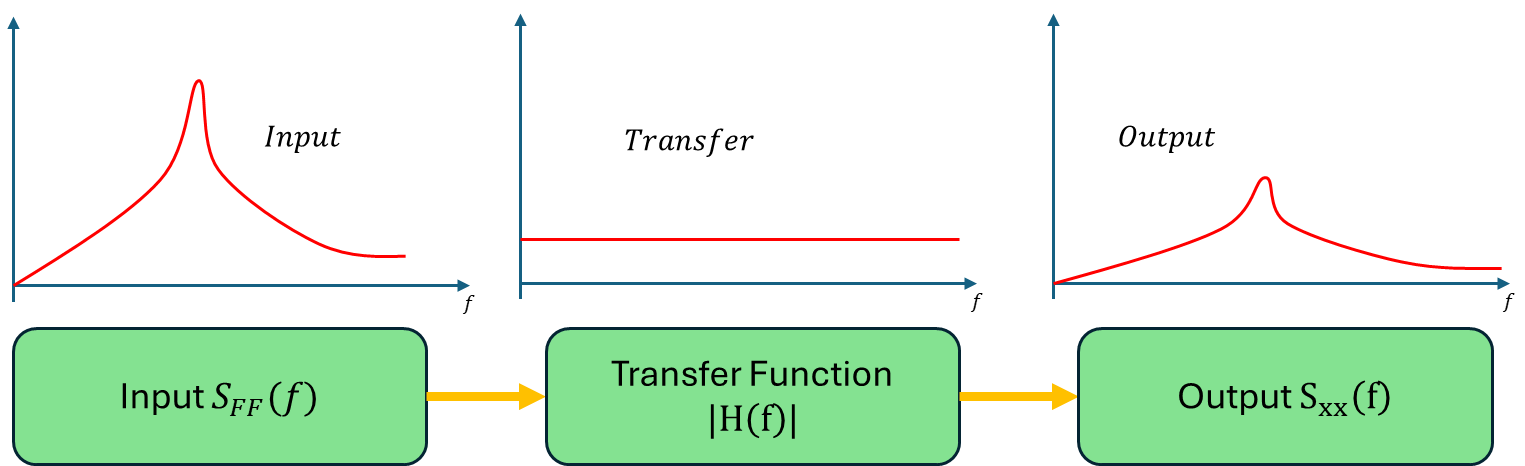
\includegraphics[width=0.75\linewidth]{Figures/Transfer.png}
    \caption{The process of using a Frequency Response Function.}
    \label{fig:FRF}
\end{figure}
Because $H(f)$ is a purely structural property, computed once from the modal
solution, it can be reused for any input \ac{PSD} at very low additional cost.
Once the displacement response \ac{PSD} is known, the stress response \ac{PSD}
at any location follows from the strain-displacement relation
(Equation \ref{eq:sigma_BDU}):

\begin{equation} \label{eq:sigma_BDU}
    \sigma = [B][D]\{u\}
\end{equation}
since [B] is the strain-displacement matrix and [D] is the material stiffness matrix.
\begin{equation}
\begin{bmatrix}
\epsilon_x \\
\epsilon_y \\
\vdots\\
\epsilon_n
\end{bmatrix}
=
[B]
\begin{bmatrix}
u_x \\
u_y \\
\vdots\\
u_{n}
\end{bmatrix}
\end{equation}


\begin{align}
    \begin{bmatrix}
        \sigma_x \\
        \sigma_y \\
        \vdots\\
        \sigma_n
    \end{bmatrix}
    =
    [D]
    \begin{bmatrix}
        \epsilon_x \\
        \epsilon_y \\
        \vdots\\
        \epsilon_n
    \end{bmatrix}
\end{align}
\newpage
\section{Random vibration analysis}
Random vibration represents a type of signal where amplitude, frequency, and phase cannot be predicted at any given time - it's non-deterministic. Unlike deterministic vibrations, such as harmonic motion, a mathematical equation cannot describe random vibration but is instead described by a \ac{PSD} \cite{33}.

\subsection{Power Spectral Density}
The \ac{PSD} describes how the power of a signal is distributed across frequency. It is usually denoted $S_{xx}$, where the subscript $xx$ indicates the type of signal, for example, the acceleration \ac{PSD} is normally denoted $S_{aa}$. The units are $EU^2/Hz$, where $EU$ stands for Engineering Unit. For acceleration, the engineering unit is normally $ms^{-2}$ or $g$.

The \ac{PSD} function shows which frequencies contain the most vibration energy. A peak in the \ac{PSD} at a particular frequency indicates significant energy content at that frequency. The area under the \ac{PSD} curve over a frequency range equals the signal's mean-square value, i.e., the square of its \ac{RMS} in that range. The \ac{RMS} is the "average" intensity of the vibration, while the \ac{PSD} is the distribution of intensity across the spectrum.

The spectral moments (not to be confused with statistical moments) are computed by Equation \ref{eq:moments}:

\begin{equation} \label{eq:moments}
    m_n = \sum^N_{i=1} f_i^n \cdot S_{\sigma, i} \cdot \delta f
\end{equation}

\subsection{Application of PSD in Fatigue Analysis}
The stress-component \ac{PSD}s for each member of the stress tensor $S$ can be computed from the frequency response, along with some structural computations, where $S = [S_{xx}, S_{yy}, S_{zz}, S_{xy}, S_{yz}, S_{xz}]$. The next step is to compute an equivalent stress \ac{PSD}, such as the von Mises or Tresca stress. There are several ways of doing this. One of the most common ways is the Segalman approach, which is described in \textit{"An Efficient Method for Calculating \ac{RMS} von Mises Stress in a Random Vibration Environment"} \cite{segalman_efficient_2000}. Another simpler method is the Halfpenny method described in \textit{"A frequency domain approach for fatigue life estimation from Finite Element Analysis"}. When a single scalar equivalent stress \ac{PSD} is computed, there are several ways to perform "Rainflow counting". Since the regular Rainflow algorithm is not useful for random vibrations, approximations of what Rainflow counting would yield from an equivalent time-domain signal are performed in the frequency domain \cite{halfpenny_frequency_1999}.

Two common methods are the Dirlik and the Steinberg methods. Both are statistical methods based on the same theory, but with different computational costs and accuracies. Once the equivalent stress \ac{PSD} and Rainflow counting are performed, the data are used in a damage model, the most commonly used of which is the Miner's Damage Model. The full chain from the multiaxial stress tensor PSD to damage and time-to-failure is summarized in Figure \ref{fig:StressToDamage}:

\begin{figure}[H]
    \begin{equation*}
        \boxed{
        \text{Multiaxial FEA}
         \rightarrow 
        S_{ss}(f)
         \xrightarrow{ \text{Segalman} } 
        S_{eq}(f)
         \xrightarrow{ \text{Dirlik or Steinberg} } 
        \dot{D},\,T_f
        }
    \end{equation*}
    \centering
    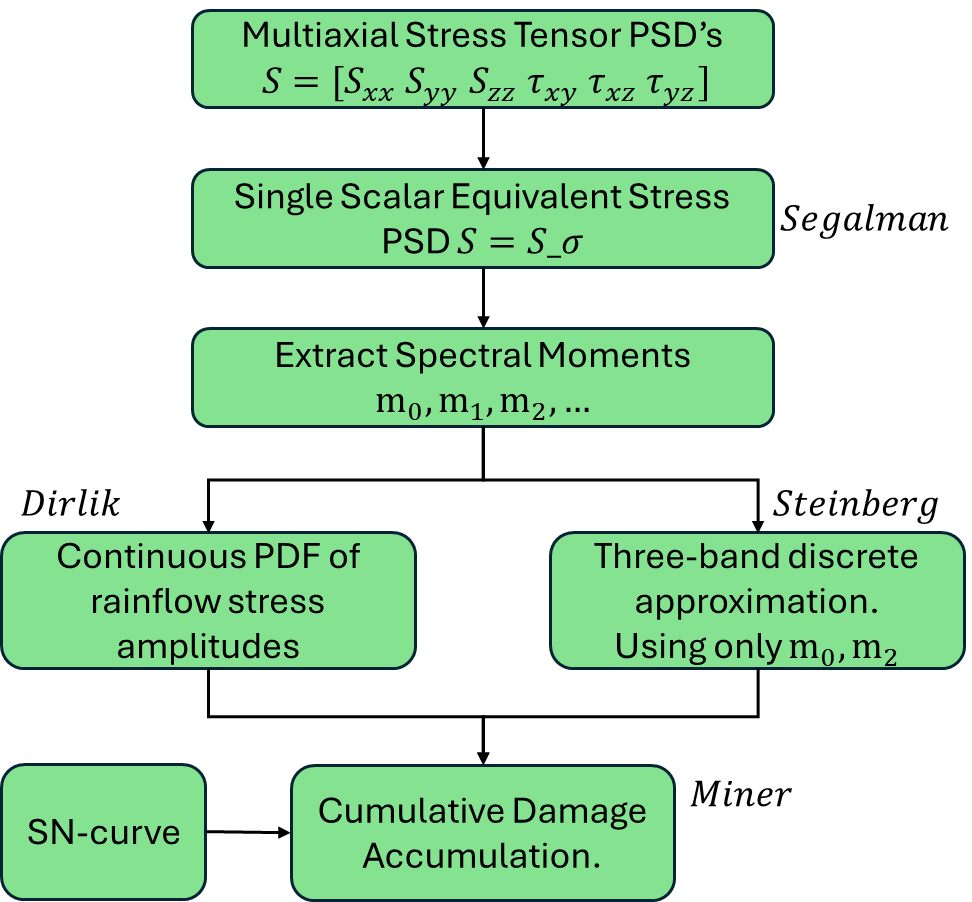
\includegraphics[width=0.75\linewidth]{Figures/StressTensorToDamage.png}
    \caption{The process of computing damage from the multiaxial stress tensor \ac{PSD}s. Note that one of Dirlik \textit{or} Steinberg would be used, not both.}
    \label{fig:StressToDamage}
\end{figure}

\subsubsection{Halfpenny method to compute Equivalent Stress PSD}
According to Halfpenny's work "A frequency domain approach for fatigue life estimation from Finite Element Analysis", the von Mises stress can be computed from the multiaxial stress \ac{PSD} tensor by
\begin{equation}
\sigma =
\begin{bmatrix}
\sigma_1 \\
\sigma_2 \\
\sigma_3 \\
\end{bmatrix}
=
eigenvalues\left\{
\begin{bmatrix}
S_{xx} & S_{xy} & S_{xz} \\
S_{xy} & S_{yy} & S_{yz}\\
S_{xz} & S_{yx} & S_{zz}
\end{bmatrix} \right\},
\end{equation}

The equivalent von Mises stress \ac{PSD} at each frequency is then computed from the principal stress \ac{PSD} values using the standard von Mises formulation applied frequency-by-frequency:
\begin{equation}
    \sigma_{VM} (f) = \sqrt{\frac{1}{2}(|\sigma_1(f) - \sigma_2(f)|^2 + |\sigma_2(f) - \sigma_3(f)|^2 +|\sigma_3(f) - \sigma_1(f)|^2 )}
\end{equation}

At each frequency, the multiaxial state is reduced to principal stresses, and the von Mises formula is applied directly. However, this frequency-by-frequency approach assumes that the principal stress directions remain constant across all frequencies, which may not always be true. At locations where different modes generate stress through different mechanisms, for example, if the first bending mode generates axial stress while a higher mode produces shear, the Halfpenny method is not valid. The Segalman approach is much more versatile, but it comes at a computational cost. The Halfpenny method is only described for completeness and is not used in the method.

\subsubsection{Segalman method to compute Equivalent Stress PSD}
The Segalman method avoids the limitations of the Halfpenny method by operating on the full Cross-Power-Spectral-Density (CPSD) matrix of stress components rather than decomposing it into principal directions.

The Segalman approach uses a quadratic form that directly maps the stress tensor \ac{PSD} to a scalar equivalent stress \ac{PSD}.

To perform the Segalman method, some variables are introduced:
\begin{enumerate}
    \item $\Psi$: Modal coordinates.
    \item p(t): von Mises stress at time t.
    \item k: Mode-index.
    \item $\sigma(t)$: stress vector of non-redundant components of the stress tensor at time t.
    \item $A_J$: Jacobian to map the stress tensor to von Mises scalar.
    \item $q_k(t)$: The $k$th modal coordinate at time t.
    \item $\Psi_k^\sigma$: Column vector of stress components $\sigma$ for mode $k$ at a specific nodal location.
    \item S: Stress tensor $S = [S_{xx}, S_{yy}, S_{zz}, S_{xy}, S_{yz}, S_{xz}]$.
\end{enumerate}

Segalman computes the stress vector function in the time domain $\sigma(t)$ by taking the sum of modal coordinates times the stress tensor column vector for each mode. The stress vector at time $t$ is then:

\begin{equation}
    \sigma(t) = \sum_k q_k(t) \Psi^\sigma_k
\end{equation}

The von Mises stress equation becomes:

\begin{equation} \label{eq:SegalmanVM}
    p^2(t) = \sigma_{xx}^2+\sigma_{yy}^2 + \sigma_{zz}^2 - (\sigma_{xx}\sigma_{yy}+\sigma_{xx}\sigma_{zz}+\sigma_{yy}\sigma_{zz}) + 3(\sigma_{xy}^2+\sigma_{xz}^2+\sigma_{yz}^2),
\end{equation}

and is the result of the quadratic form in the stress components:
\begin{equation}
p^2(t) = \sigma^T(t) A_J \sigma(t)
\end{equation}

where $A_J$ is a constant $6 \times 6$ coefficient/Jacobian matrix that transforms the stress tensor to the von Mises stress. For the standard von Mises definition that is given by Equation \ref{eq:SegalmanVM}, $A_J$ has the form:

\begin{equation}
A_J =
\begin{pmatrix}
1 & -0.5 & -0.5 & 0 & 0 & 0 \\
-0.5 & 1 & -0.5 & 0 & 0 & 0 \\
-0.5 & -0.5 & 1 & 0 & 0 & 0 \\
0 & 0 & 0 & 3 & 0 & 0 \\
0 & 0 & 0 & 0 & 3 & 0 \\
0 & 0 & 0 & 0 & 0 & 3
\end{pmatrix}
\end{equation}

\subsubsection{Dirlik method to perform Rainflow counting in the frequency domain}
The Dirlik method builds a semi-empirical \ac{PDF} to approximate rainflow counting. The \ac{PDF} is given by Equation \ref{eq:Dirlik}:

\begin{equation} \label{eq:Dirlik}
    p(S) = \frac{1}{2\sqrt{m_0}} \big( \frac{D_1}{Q}e^{-\frac{Z}{Q}} + \frac{D_2Z}{R^2}e^{-\frac{Z^2}{2R^2}}+D_3Ze^{-\frac{Z^2}{2}} \big),
\end{equation}
where the variables are defined by:
\begin{enumerate} % 
    \item $x_m = \frac{m_1}{m_0} \sqrt{\frac{m_2}{m_4}}$
    \item $\nu_p = \sqrt{\frac{m_4}{m_2}}$ (peak rate), $\nu_0 = \sqrt{\tfrac{m_2}{m_2}}$ (zero-upcrossing rate)
    \item $\gamma = \frac{\nu_0}{\nu_p} = \frac{m_2}{\sqrt{m_0m_4}} = \frac{\text{number of upward zero crossings}}{\text{number of peaks}}$ (Irregularity ratio).
    \item $R=\frac{\gamma-x_m-D_1^2}{1-\gamma-D_1+D_1^2}$
    \item $Z = \frac{S}{2\sqrt{m_0}}$
    \item $D_1 = \frac{2(x_m-\gamma^2)}{1+\gamma^2}$, \quad $D_2 = \frac{1-\gamma - D_1+D_1^2}{1-R}$, \quad $D_3 = 1-D_1-D_2$
    \item $Q = \frac{1.25(\gamma-D_3-D_2R)}{D_1}$
\end{enumerate}


\begin{figure}[H]
    \centering
    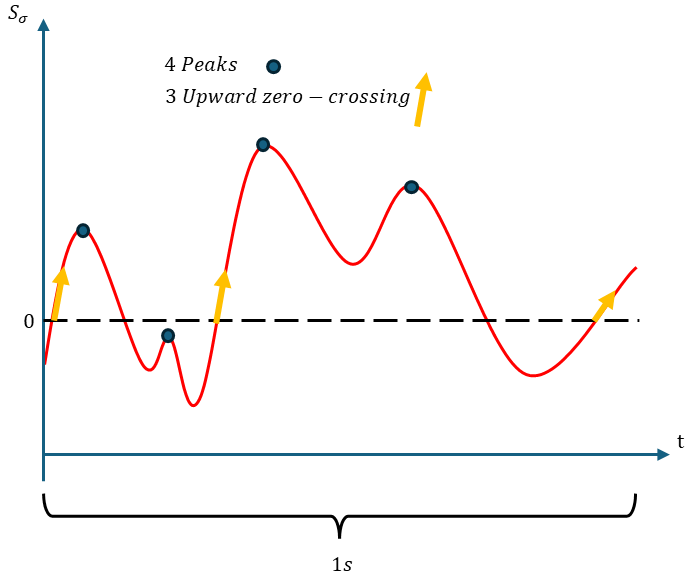
\includegraphics[width=0.6\linewidth]{Figures/Peaks.png}
    \caption{The spectral moments used in the Dirlik method.}
    \label{fig:DirlikMoments}
\end{figure}

Once $p(S)$ is known, the expected damage during the exposure time $T$ is according to Equation \ref{eq:damage}:

\begin{equation} \label{eq:damage}
    D = \nu_p T\int^\infty_0 \frac{p(S)}{N_f(S)}dS.
\end{equation}

With an SN-curve written as $N_f(S) = C S^{-m}$, the damage per time is computed using the Miner's rule:
\begin{equation}
    \dot{D} = \nu_p \int^\infty_0 \frac{S^m}{C}p(S)dS
\end{equation}

The fatigue life is $T_f = \tfrac{1}{\dot{D}}$.

\subsubsection{Steinberg method to perform Rainflow counting in the frequency domain}
The Steinberg method does not compute a specific \ac{PDF}, but assumes a Gaussian distribution of stress cycles, and uses stress levels derived from the \ac{RMS} stress response. This means that:

\begin{itemize}
    \item 68.27 \% of cycles fall within the $\pm 1\sigma$ band (one standard deviation, $k=1$) stress level,
    \item 27.18\% of cycles fall within the $\pm 1\sigma$ to $\pm 2\sigma$ band (two standard deviations, $k=2$) stress level and
    \item 4.28 \% fall within the $\pm 2\sigma$ to $\pm 3\sigma$ band (three standard deviation, $k=3$) stress level.
\end{itemize}
The three ratios sum up to $68.27 + 27.18 + 4.28 = 99.73 \%$, the remaining $0.27 \%$ of cycles that exceed the $3\sigma$ level are neglected. This "Three-band technique" makes the Steinberg method much more computationally justifiable than continuous \ac{PDF} methods.

The number of cycles within each stress level $k\cdot\sigma$, where $k = 1, 2, 3$, depends on the statistical frequency $f_0$ and the exposure time $T$. For example, the number of cycles at or below the $1\sigma$ level is
\begin{equation}
    n_{1\sigma} = 68.27\%\cdot f_0 \cdot T.
\end{equation}
The statistical frequency is computed as
\begin{equation} \label{eq:statisticalFrequency}
    f_0 = \frac{1}{2\pi} \frac{\dot{\sigma}_{RMS}}{\sigma_{RMS}} = \frac{1}{2\pi} \sqrt{\frac{m_2}{m_0}},
\end{equation}
where $\dot{\sigma}_{RMS}$ is the \ac{RMS} of the stress rate, and $\sigma_{RMS}$ is the \ac{RMS} stress.

The total damage is then computed with Miner's rule for the three bands:
\begin{equation}
    D = \frac{n_{1\sigma}}{N_{1\sigma}} + \frac{n_{2\sigma}}{N_{2\sigma}} + \frac{n_{3\sigma}}{N_{3\sigma}},
\end{equation}
where $N_{k\sigma}$ is read from the SN-curve at stress level $k\cdot \sigma_{RMS}$.

\subsubsection{Mean Stress Correction}
Most standard fatigue analysis methods assume the mean stress is zero, but this is rarely true. Especially for a bolted joint, a pretension is already determined. Therefore, an equivalent "zero-mean" stress must be computed, and there are different ways of doing this here as well. Two common ways to perform mean stress correction are the Goodman and Gerber models \cite{budynas_shigleys_2015}. Both are based on the same variables and the same theory, but with different approaches. The relationship in Equation \ref{eq:Goodman} explains the linear Goodman curve, and Equation \ref{eq:Gerber} explains the quadratic Gerber curve. Both are seen in Figure \ref{fig:Haigh}.

\begin{equation} \label{eq:Goodman}
    \frac{S_a}{S_e} + \frac{S_m}{S_u} = 1,
\end{equation}

\begin{equation} \label{eq:Gerber}
    \frac{S_a}{S_e} + \left(\frac{S_m}{S_u}\right)^2 = 1,
\end{equation}

where for Random Vibrations the mean stress $S_m$ is determined by the stress before the random response, i.e., the static load. In a bolt, it is equal to the bolt pretension divided by the bolt tensile stress area, which is not equal to the cross-sectional area but instead either taken from tables or computed using Equation \ref{eq:TensileStressArea}. The alternating stress $S_a$ is derived from the stress \ac{PSD}, if using Steinberg, it is one of $1\sigma$, $2\sigma$, or $3\sigma$ \ac{RMS} stress levels.

If the Dirlik approach is being used, the mean stress correction is typically applied by modifying the fatigue coefficient $C$ before calculating the expected damage rate. This yields an effective fatigue coefficient $C_{eff}$ that accounts for the static preload.

\begin{figure}[H]
    \centering
    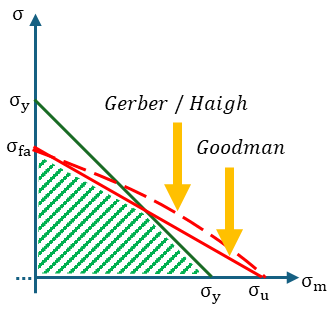
\includegraphics[width=0.5\linewidth]{Figures/Haigh.png}
    \caption{Illustration of the difference in Gerber and Goodman formulations. Goodman is simpler and more conservative. Conditions within the striped area are not subject to fatigue failure, but may still exhibit other effects from random vibration.}
    \label{fig:Haigh}
\end{figure}

\subsubsection{Miner Damage Model in the frequency domain}
Miners' rule has been mentioned and used in the explanation of the "rainflow approximation methods", but also deserves its own section. Miner's rule is a theory of damage accumulation under variable-amplitude loading. It claims that the sum of ratios of cycles per the fatigue life at some amplitude determines the total damage, as seen in Equation \ref{eq:miners}:

\begin{equation} \label{eq:miners}
    D = \sum_i \frac{n_i}{N_i}
\end{equation}

where $n_i$ is the number of cycles experienced, and $N_i$ is the number of cycles to failure at the ith stress amplitude level. Fatigue failure is predicted when $D\ge 1$.

The Sandia report refers to Bannantine's work "Fundamentals of Metal Fatigue Analysis" \cite{bannantine_fundamentals_1990}, and explains that the theory is generally accurate, but can in some cases be non-conservative.
\begin{quote}
    \textit{"Bannantine notes that Miner's rule can be non-conservative for two-level tests where the initial level is a high amplitude and the second level is a low amplitude. Bannantine also notes that tests using random histories with several stress levels show very good correlation with Miner's rule."} - Sandia National Laboratories \cite{Sandia}.
\end{quote}
The non-conservativeness stems from the assumption that the damage contribution from each stress cycle is independent of the loading sequence. For random vibrations, the stress history is not deterministic and should not be interpreted as a set of independent constant-amplitude cycles taken directly from individual \ac{PSD} frequency bins. A stress \ac{PSD} describes how the variance of the stress is distributed over frequency. Spectral fatigue methods therefore first reduce the \ac{PSD} to spectral moments and characteristic rates, such as the zero-upcrossing rate and peak rate (Figure \ref{fig:DirlikMoments}). These quantities are then used to estimate an expected stress range or stress amplitude distribution. Fatigue damage is computed from this expected distribution using Miner's rule (Equation \ref{eq:stressCycles}). Dirlik's method estimates the probability density of the rainflow range from spectral moments and combines it with the SN-curve to obtain an expected damage rate.

\begin{equation}\label{eq:stressCycles}
    N_1 = N_r\left(\frac{\sigma_r}{k\sigma_1}\right)^b
\end{equation}

where
\begin{itemize}
    \item $N_1$ is the number of cycles to failure at the $1\sigma$ \ac{RMS} stress value $\sigma_1$.
    \item $N_r$ is the number of cycles to failure at a reference point, usually $N_r = 10^3$.
    \item $\sigma_1$ is the $1\sigma$ (one standard deviation) \ac{RMS} stress from the frequency analysis.
    \item $\sigma_r$ is the stress to fail at a the reference point $(N_r; \sigma_r)$.
    \item $b$ is the slope in log-log scale of the SN-curve.
    \item $k$ is the number of standard deviations - k=1 means $1\sigma$.
\end{itemize}

The three regions of the SN-curve and the fatigue limit FL separating finite-life from infinite-life behavior are illustrated in Figure \ref{fig:SN-curve}:


\begin{figure}[H]
    \centering
    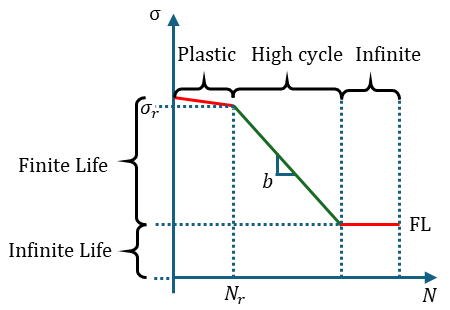
\includegraphics[width=0.75\linewidth]{Figures/SN-curve.png}
    \caption{SN-curve showing the three fatigue life regions. The slope b in the finite-life (high-cycle) region, FL, is the fatigue limit separating finite-life from infinite-life behavior.}
    \label{fig:SN-curve}
\end{figure}

Since the frequency $f_i$ at which a certain \ac{PSD} stress magnitude $S_{\sigma, i}$ occurs is known from the \ac{PSD} analysis, the time exposure $T_{exp}$ can be used to determine the actual number of fatigue cycles $n_i$:
\begin{equation} \label{eq:n_sigma}
    n_i = f_i \cdot T_{exp}
\end{equation}

Substituting Equation \ref{eq:n_sigma} and \ref{eq:stressCycles} into miners' rule in Equation \ref{eq:miners}, we get the following equation for damage in a structure that is subjected to random vibration fatigue:
\begin{align}
    D &= \sum_{i=1}^j \frac{n_i}{N_i}\\
      &= \sum_{i=1}^j \frac{f_iT_{exp}\cdot (k\sigma_i)^b}{N_r \sigma_r^b}  \\
      &= \frac{T_{exp}k^b}{N_r\sigma_r^b}\cdot \sum_{i=1}^j f_i\sigma_i^b \label{eq:PSD_Damage}
\end{align}

Equation \ref{eq:PSD_Damage} shows that the damage is dependent on the time exposure $T$, parameters from the SN-curve ($N_r$, $\sigma_r$, $b$), and the number of standard deviations $k$, along with the sum of products frequency times stress \ac{RMS} to the power of $b$.

\begin{equation}
    \dot{D} = \frac{D}{T_{exp}} f= \frac{k^b}{N_r\sigma_r^b}\cdot \sum_{i=1}^j f_i\sigma_i^b
\end{equation}

\section{Stress Concentration Factors} \label{sec:SCF}

According to \textit{"Numerical and theoretical studies of bolted joints under harmonic shear displacement"} by Liu \textit{et al.}, the stress concentration factor varies with thread type. In their computational analysis, they found that, for their specific model, the stress concentration factors were $4$ for the first thread, $2$ for the second, $1.5$ for threads 3-6, and $1$ for the seventh used thread. This means that the first active thread experiences $400 \%$ of the nominal stress \cite{liu_numerical_2015}.


The NASA report \textit{"Stress Concentrations in Screw Threads"} by G. Peter O'Hara shows that Heywood's equation matches results from fully detailed Nastran models \cite{ohara_stress_nodate}. This theory is presented here for completeness. It requires detailed thread geometry that is not part of the threadless solid bolt model used in this thesis. The cross-validation in Section \ref{sec:validity}, therefore, used the tabulated \ac{SCF} $K_t = 3.8$ from Shigley rather than computing Heywood's formula numerically. The Heywood equation is a semi-empirical equation that is defined by Equation \ref{eq:Heywood}:

\begin{equation} \label{eq:Heywood}
    \sigma_F = \left[1 + 0.26\left(\frac{e}{R}\right)^{0.7}\right]\cdot \left[ \frac{1.5a}{e^2} + \sqrt{\frac{0.36}{be}} (1+\frac{1}{4})sin(\gamma) \right] \frac{W}{T}
\end{equation}

According to Brennan (\textit{"Fatigue and Fracture Mechanics Analysis of Threaded Connections"}), the Heywood formulation of \ac{SCF} is derived from studies of tensile fillet stresses in loaded projections \cite{brennan_fatigue_nodate}. He found that the proximity of the applied load to the fillet significantly affected the tensile stresses and derived an empirical formula of the form:

\begin{equation}
    K_{T, total} = K_{T, bend} + \frac{K_{T, \sigma}}{\sqrt{1 + constant\cdot K_{T, \sigma}}},
\end{equation}
where the value of the constant differs for various thread forms. A parametric equation for the stress concentration factor was derived as a function of pitch, tooth height, wall thickness, and the fraction of the overall applied load carried by the tooth.

The approach that Brennan explains follows:
\begin{enumerate}
    \item Compute axial load on the thread ($F_S = \Phi\cdot F_L \rightarrow F_{tooth} = \alpha_1F_S$), where $\alpha_1$ is the load fraction carried by the first engaged thread, typically $\sigma_1 \approx 0.30 - 0.38$ according to Sopwith's thread load distribution \cite{brennan_fatigue_nodate}.
    \item Compute the thread-root \ac{SCF} using Heywoods formula ($K_{T, total}$).
    \item Combine preload and dynamic axial load, the total local stress at the first engaged thread is $\sigma_{local} = K_{T, total} \cdot \frac{F_{tooth}}{A_{thread\; root}}$.
\end{enumerate}


This is also compliant with \textit{Shigleys Mechanical Engineering Design}, where table 8-16 states that the stress concentration of metric threaded fasteners is 3.0 for rolled threads and 3.8 for cut threads of metric grade 10.9 \cite[p.437]{budynas_shigleys_2015} (rolled and cut are manufacturing techniques for bolts). They also provide a stress concentration factor of 2.3 for the under-head fillet.


\section{Finite Element Analysis} \label{sec:FEA}
When the \ac{FEM} is used to perform an analysis, the resulting analysis is called a Finite Element Analysis (FEA). It is a method for discretizing complex equations into a set of simpler equations that together define a distribution that approximates the original equation.

The accuracy and cost of the analysis depend on the element type, mesh density, the mathematical model, and the contact assumptions. Real-world responses are generally nonlinear, whereas many efficient analyses (such as frequency response) assume linearity. The prestressed linear perturbation method handles this by first running a nonlinear static step to establish the preloaded contact state, then linearising the system about that step for subsequent dynamic analyses. 

The choice of how to represent the bolt itself substantially changes both the cost and the response quantities the model can produce.

\subsection{Bolt representations in FEA}
\textbf{Bonded surface representation.} The bonded surface representation bolt is replaced by a rigid bond between the clamped members at the bolt-hole interfaces, with no bolt body present in the model. There is no bolt geometry to extract stress from, and no degree of freedom for friction. Preload is applied as a tensile traction between the bonded surfaces. The bonded representation cannot capture phenomena that depend on bolt-body stress or relative motion between the clamped members.

\textbf{beam representation.} The bolt shank is represented by a CBAR beam element with the cross-sectional properties of the shank (area, second moment of area, polar moment). The beam is connected to the clamped members at the head and nut-bearing surfaces, typically via rigid couplings or distributed coupling elements. The beam captures the axial and bending responses of the shank with very low computational cost, but does not resolve local stress concentrations at the head fillet or the threads.

\textbf{CBUSH representation.} A scalar CBUSH element is a 6-\ac{DOF} spring. Each of the six stiffness coefficients (three translational, three rotational) is assigned according to a derivation procedure described in Section \ref{sec:CBUSH_Stiffness}. The CBUSH representation is even cheaper than the beam but lacks a physical bolt body and therefore cannot directly produce bolt-region stresses.

\textbf{Threadless 3D solid representation.} The bolt is modeled using three-dimensional solid elements that resolve the head, shank, and nut geometry, but the shank is modeled as a smooth cylinder without any threaded geometry. Preload is applied as a tensile load across a cut section in the shank. The threadless solid captures bolt-body stresses, including head-fillet stress concentration, but it cannot capture thread-root stress concentration or thread-engagement load distribution.

\textbf{Fully threaded 3D solid.} A complete representation with threaded geometry, frictional thread contact, and frictional contact at the nut bearing surface. It is included in the phenomenon-method matrix because it is the only representation capable of capturing thread-root SCFs, thread loosening, and stage-2 self-loosening, but it is not part of the four-model computational benchmark.

\section{Vibration test standards} \label{sec:standards}
Two standards are used in this thesis to define the random vibration input. These are described in Subsection \ref{NASA} and \ref{T43A}.

\subsection{NASA-STD-7001B} \label{NASA}

The NASA-STD-7001B (Payload Vibroacoustic Test Criteria) establishes testing requirements for spaceflight hardware, providing acceleration \ac{PSD} specifications that define minimum test levels across different frequency ranges \cite{NASA_STD_7001B_2017}.

\subsection{MIL-STD-810G} \label{T43A}

The MIL-STD-810G, Method 514.6 (Vibration), defines vibration exposure environments for military equipment.
It provides \ac{PSD} profiles organized by vehicle category (common carrier trucks, wheeled vehicles, aircraft), derived from field measurements \cite{MIL_STD_810G_2008}.

Both standards express the vibration environment as acceleration \ac{PSD} curves, making them directly applicable as input to the frequency-domain analysis chain adopted in this thesis.

\chapter{Related Work} \label{chp:relatedwork}

Research on bolted joints is a vital area within structural and mechanical engineering. Yet, a significant gap is found in the review of related work. There is no universal, efficiency-aware guideline for selecting a bolt modeling strategy in finite element analysis for random-vibration fatigue. The literature presents different bolt modeling approaches: bonded contacts, beam elements, 3D solids without threads, and 3D solids with threads, each with different accuracy and cost.

\section{Submodelling techniques}
In \textit{"Analysis of the stress and load distribution of an assembled screw including threaded contact"} by C. Hollenbeck, he used a 3D solid bolt model with threads and also a 2D axisymmetric model with threads. He accounted for material nonlinearity and all mechanical contacts. He compared the results of 3D solid threads and 2D threads \cite{Hollenbeck2023AssembledScrew}.


\section{Bolt modeling fidelity and the accuracy-cost Trade-Off}
\label{sec:bolt-modeling}

The \ac{FEA} of bolted joints involves a fundamental trade-off between model fidelity and computational cost. High-fidelity models that represent the bolt, nut, and clamped members using three-dimensional solid elements can capture complex nonlinear contact phenomena, including slipping, joint opening, and preload loss under dynamic loading \cite{Hollenbeck2023AssembledScrew}, \cite{27}. Ahmad \textit{et al.}, for instance, used 3D \ac{FEA} with the Extended Finite Element Method (XFEM) to predict bearing strength and failure modes in composite joints \cite{01}, demonstrating that detailed solid models can serve as an accuracy baseline, but for structures that contain many fasteners, full solid modeling becomes computationally expensive. Simplified techniques using beam elements, springs, or bonded contacts have therefore been developed.



Hollenbeck compared a fully detailed 2D axisymmetric thread model with a simplified 3D thread for a single screw. Material nonlinearity and all mechanical contact pairs were included.
The comparison showed that geometric thread fidelity measurably affects the head-fillet stress concentration and the load distribution along the engaged threads, and that 2D axisymmetric models reach a level of detail impractical to mesh in 3D \cite{Hollenbeck2023AssembledScrew}.

Kim \textit{et al.} compared four modeling configurations - solid bolt, coupled bolt, spider bolt, and no-bolt models - and validated them against static experiments and modal tests \cite{27} on a single-bolt specimen. They found that the solid bolt model yields the most accurate stress and dynamic response. Still, the coupled bolt model achieves similar global behavior while requiring significantly less computational time and memory. This study is directly relevant to this thesis because it demonstrates that bolt representation can trade accuracy for cost. However, Kim \textit{et al.} limited their work to static loading and did not consider random-vibration fatigue. The geometry used in this thesis is directly taken from this reference, see Section \ref{chp:method} and Figure \ref{fig:Drawing1}.

Kang \textit{et al.} extended this accuracy-cost question to random fatigue loading, comparing a solid bolt model with a simplified bolt model on a wind turbine. They confirmed that the simplified bolt representation is significantly more efficient in computational time and memory, and used it with an SN-curve and the Palmgren-Miner linear damage rule to predict fatigue life under random loads. Their work supports the use of simplified bolt representations for global fatigue assessment, but used a single load case and does not benchmark several fidelities against each other \cite{10}.

Naruse and Shibutani \cite{09} used 3D \ac{FE} models of bolted joints to evaluate the equivalent axial and bending stiffness of the clamped plates and compared the results with the VDI 2230 analytical prediction. They found that VDI 2230 gives slightly larger stiffness than the \ac{FE} results, which makes evaluations based on the standard non-conservative for the bolt internal force. A simplified shell-and-beam modeling technique that builds on the same VDI compliance framework was developed in earlier work by the same group \cite{07}. Ding and Elkady found in \textit{"Generalized spring model for steel bolts in tension considering uncertainty and loading speed"} that the VDI 2230 stiffnesses could be as much as 50 - 70 \% higher than experimental data \cite{ding_generalized_2025}. This finding is important for the present work because it motivates using \ac{FEA} as a complement to analytical baselines rather than only replicating them.

Omar \textit{et al.} addressed the same problem from a model-updating perspective. They proposed two \ac{FE} representations of a bolted joint structure for predicting dynamic behavior and updated their parameters against experimental modal data, showing that the choice of element type at the joint location strongly affects the predicted natural frequencies even after updating \cite{noauthor_pdf_2025}.

An \textit{et al.} reviewed fatigue behavior and failure modes in composite and metal bolted joints \cite{08}. Their review covers a broad range of theoretical models but does not address the trade-off between computational efficiency and prediction accuracy in sufficient detail to support a decision framework.

According to \textit{Handbok om skruvförband} \cite{Colly}, the external load is generally not applied at the surface of the clamped members but somewhere inside them, which causes a decrease in internal residual clamp force in the joint.

\paragraph{Relation to this thesis.}
The studies above establish that different bolt representations produce different accuracy and cost outcomes. However, none of them quantify this trade-off using a single efficiency metric, nor do they extend the comparison to random-vibration fatigue loading. This thesis addresses both gaps by defining an \textit{Efficiency Ratio} $\eta$, evaluating it across four bolt modeling representations under \ac{PSD} excitation, and guiding the user in selecting a model that adequately captures all critical phenomena at acceptable cost.


\section{Spectral fatigue life prediction methods}
\label{sec:spectral-fatigue}

Frequency-domain fatigue methods avoid the computational expense of time-domain cycle counting by deriving a stress amplitude \ac{PDF} directly from the stress \ac{PSD}. All spectral methods rely on the spectral moments $m_0, m_1, m_2, m_4$ of the stress \ac{PSD} to calculate the expected zero-crossing and peak rates. The cumulative damage is then computed using the Palmgren-Miner linear damage rule in combination with the material SN-curve.

Halfpenny reviewed some frequency-domain fatigue methods, including the Steinberg and Dirlik approaches that are used in this thesis. He showed, by comparison with rainflow-counted time-domain results, that the Dirlik method yields the closest agreement across narrow- and broadband-\ac{PSD} cases \cite{halfpenny_frequency_1999}. Demirel and Kayran provided a detailed implementation of the Dirlik damage model for vibration fatigue analysis \cite{72}. Together, these two references provide the algorithmic basis for the fatigue post-processing used in the present thesis.

For multiaxial random vibration, the 6x6 stress \ac{PSD} tensor must be reduced to a scalar equivalent before a spectral method can be applied. Segalman \textit{et al.} derived an efficient expression for the \ac{RMS} von Mises stress in linear structures excited by random loads, expressed in terms of the auto- and cross-spectral densities of the stress components \cite{segalman_efficient_2000}. 

\paragraph{Relation to this thesis.}
The reviewed spectral methods form the fatigue post-processing stage of the analysis chain used in this work. The Segalman von Mises is used to construct the equivalent stress \ac{PSD}, the spectral moments are computed from that \ac{PSD}, and the Dirlik method is then applied to all four bolt representations. By keeping the algorithm constant across all four bolt representations and load cases, this thesis isolates the effect of bolt representation on the predicted fatigue life.

\section{Experimental validation of nonlinear joint dynamics}
\label{sec:experimental}

Roettgen \textit{et al.} conducted an experimental-analytical study using the Brake-Reuß Beam to validate two approaches for predicting the dynamic behavior of structures with nonlinear joints in \textit{"Substructuring of a nonlinear beam using a modal Iwan framework Part I"} and \textit{Part II}.
The first approach was a finite element model with discrete Iwan joints. Three separate Iwan elements (nonlinear elements designed to reproduce bolt slip) were placed at the bolt locations, each described by four parameters calibrated by comparing model predictions with measurements of the physical structure.
The second approach was experimental-analytical substructuring with modal Iwan models. Modal testing on the physical model with the same geometry yielded the first two elastic modes of vibration, each fitted with an Iwan element that captures the modal response as a function of amplitude. Coupling these Iwan modal models enabled accurate prediction of the response \cite{allen_substructuring_2025}, \cite{roettgen2017substructuringPartII}.

Brake \textit{et al.} review the state of the art in modeling friction and slip in jointed structures in \textit{"Testing and Modeling of Friction and Slip in Mechanical Interfaces: State of the Art and Perspectives for the Next Decade"}, and found that jointed interfaces can strongly affect the nonlinear dynamics of structures even though the relevant contact features are much smaller than the global structure \cite{brake_testing_2024}. In particular, they noted that bolted lap joints typically exhibit only weak stiffness nonlinearities, seen as small amplitude-dependent shifts in natural frequency, but much stronger nonlinear damping due to frictional micro-slip at the interface. This behavior was illustrated by a reduction in natural frequency of approximately 1-2\% and an increase in damping of roughly 5-10 times the low-amplitude value. This supports the use of Iwan-type models, which are well-suited to capturing micro-slip behavior, while also highlighting that macro-slip, wear evolution, and the underlying interface physics remain difficult to validate and remain open challenges in joint modeling.

Lacayo \textit{et al.} compared a time-domain whole-joint Iwan approach (a single lumped Iwan element representing the global nonlinear response of the entire bolted joint, rather than one Iwan element per node-pair) with a frequency-domain multi-harmonic balance approach for the Brake Reuß Beam in \textit{"Nonlinear modeling of structures with bolted joints: a comparison of two approaches based on a time-domain and frequency-domain solver"} and found that the two methods predict the experimental nonlinear response with comparable accuracy \cite{15}. This supports the broader use of frequency-domain solvers for jointed-structure dynamics. However, both methods are nonlinear and therefore complement rather than directly justify the linear prestressed modal analysis used in the present thesis.

%Similar work was made in \textit{"Testing and Modeling of Friction and Slip in Mechanical Interfaces: State of the Art and Perspectives for the Next Decade"} by Brake \textit{et al.}, where they found that ... \cite{brake_testing_2024}. Lacayo \textit{et al.} compared time-domain and frequency-domain nonlinear joint models for the BRB \cite{15}, directly supporting the use of frequency-domain methods and pre-stressed modal analysis for bolted-joint dynamics.

\paragraph{Relation to this thesis.}
The Iwan-based approaches capture amplitude-dependent damping and stiffness, phenomena that are \textit{not} represented by the method used in this thesis.

The comparison between the linear perturbation results of this thesis and the nonlinear experimental data from Roettgen \textit{et al.} and Lacayo \textit{et al.} \cite{15}, therefore, provides a natural validity boundary. When the excitation amplitude is large enough for micro-slip and contact-state changes to dominate the response, the linear perturbation assumption becomes inadequate, and nonlinear time-domain methods are required.

\section{Analytical baselines} \label{Analytical_Standards}
The VDI 2230 is a standard that provides a systematic calculation framework for bolted joints, including the equivalent cone model for clamped-member compliance, the torque-tension relationship, and the load factor \cite{VDI}. As discussed, several \ac{FE} studies have shown that VDI 2230 over-replicates axial stiffness by a margin large enough to be relevant for fatigue assessment \cite{09}, \cite{ding_generalized_2025}.

The Sandia guideline (SAND2008-0371) reviews three clamped-member stiffness models the Bickford Q-factor approach, the VDI conical frustum, and the \ac{DMP} correlation and recommends DMP for its close agreement with detailed axisymmetric \ac{FE} results across a wide range of joint geometries \cite{Sandia}. The DMP method is used in this thesis to derive the axial CBUSH stiffness $K_3$ for the CBUSH model (see Chapter \ref{chp:method}).

\paragraph{Relation to this thesis.}
The VDI 2230 stiffness and preload calculations, together with the Sandia DMP, provide the analytical equations used for the stiffnesses in the CBUSH bolt representation. The vibration test standards supply the \ac{PSD} load cases that drive the dynamic analysis and, ultimately, the fatigue life prediction.

\section{Summary and research gap}
\label{sec:summary}

The following sections show that individual elements of the bolt-fatigue-FEA problem are well covered in the literature:
\begin{enumerate}
    \item Spectral fatigue methods (Halfpenny, Dirlik, Segalman, Steinberg)
    \item Bolt modeling fidelity is static and modal analysis (Kim \textit{et al.}, Naruse \textit{et al.}, Omar \textit{et al.})
    \item Experimental characterization of nonlinear joint dynamics (Lacayo \textit{et al.}).
    \item Test standards and analytical frameworks provide both the loading environment and the stiffness/ preload references needed for verification.
\end{enumerate}

No existing study, however, systematically maps physical phenomena in bolted joints under random vibration to the cheapest adequate FE-model, nor provides a quantitative accuracy-cost indicator for that mapping. This thesis reduces that gap in three ways:
\begin{enumerate}
    \item By testing four bolt representations of different fidelity: Bonded, Beam, CBUSH, and threadless Solid.
    \item By reducing the results to a phenomenon-method matrix and a decision flowchart
    \item By quantifying the accuracy-cost trade-off across two standardized random-vibration profiles and two loading directions.
\end{enumerate}

The work establishes effective methods for simplified stiffness modeling \cite{07} and different fatigue life predictions under random loads \cite{03, 10, segalman_efficient_2000, 72}. However, no study in the reviewed literature quantifies the trade-off between bolt modeling fidelity and predictive accuracy \textit{specifically} for random vibration fatigue.

While Kim \textit{et al.} compared bolt models under static and modal conditions \cite{27}, Demirel and Kayran \cite{72}, and Segalman \textit{et al.} \cite{segalman_efficient_2000} demonstrated spectral fatigue methods, a computational framework that defines an Efficiency Ratio weighing pre-processing effort and solver cost against accuracy in the frequency domain has not been proposed. This thesis reduces the identified gap by combining the Bonded, Beam, CBUSH, and threadless Solid bolt representations with the spectral fatigue analysis chain and evaluating them under two different acceleration \ac{PSD} loadings.

The literature demonstrates substantial expertise in bolted-joint design, preload analysis, and fatigue assessment under dynamic loading. It also shows that several modeling strategies are available. However, the reviewed work does not provide clear engineering guidelines for selecting model fidelity in \ac{FEA},  specifically for random-vibration fatigue applications. In particular, there is a lack of practical guidance that relates 1) the physical phenomenon of interest, 2) the required modeling fidelity, and 3) the resulting trade-off between computational cost and predictive accuracy. Addressing this gap is the main contribution of this thesis.

In summary, the literature provides information about all three problems: 1) Analytical bolt-stiffness, 2) Spectral fatigue damage, and 3) Non-linear joint dynamics under test standards.

% \begin{enumerate}
%     \item Analytical bolt-stiffness,
%     \item Spectral fatigue damage,
%     \item Non-linear joint dynamics under test standards.
% \end{enumerate}
It does, however, not bring them together into a systematic comparison of competing finite-element bolt representations for random-vibration fatigue in terms of accuracy and cost. The specific gap that this thesis addresses is the lack of a quantitative, reproducible method for selecting a finite-element bolt representation based on the physical phenomenon of interest, the required fatigue accuracy, and the computational cost of the simulation.

The thesis reduces this gap in two ways. First, it constructs a phenomenon-method matrix that maps relevant physical phenomena to the minimum useful model fidelity and to analysis based on prior theory and literature. Second, it constructs a four-model comparative computational experiment (Chapter \ref{chp:method}) that evaluates each model against a solid reference under two standardized \ac{PSD}s and two loading directions (Chapter \ref{chp:results}). Together, these two parts provide a structured basis for engineering model selection before any simulations are run.



\chapter{Method}
\label{chp:method}
The method in this thesis combines a qualitative, literature-based capability map with a quantitative, comparative finite-element benchmark. The capability map identifies which physical phenomena in bolted joints under random vibration require which analysis type and model fidelity. The quantitative part evaluates several bolt modeling strategies against each other with respect to both computational efficiency and fatigue-relevant response in the present single-bolt benchmark. The two parts are related but not evidently identical: the first provides a capability map, while the second provides a controlled numerical comparison. Both are used to support the decision aids that are the phenomenon-method matrix (Table \ref{tab:phenomenaMethodMatrix}), and the decision flowchart (Figure \ref{fig:decisionTree}).

The method is designed to answer the Research Question:

\begin{quote}
    \textit{\RQ}
\end{quote}

and to reject or confirm the hypothesis:

\begin{quote}
    \textit{\HYP}
\end{quote}

The study is designed as a comparative computational experiment, in which controlled variables (bolt fidelity) are tested to observe dependent variables, such as solver time and frequency-domain stress accuracy. The primary contribution from this thesis is a two-part decision aid for resource-efficient \ac{FEA} of bolted joints under random vibration: a literature-based phenomenon-method matrix and a benchmark-based comparison of model accuracy versus computational cost for the present fatigue problem.

\newpage
\section{Research method}

The method consists of two complementary parts: a qualitative study and a quantitative benchmark study.

The qualitative part is a literature- and theory-based study that identifies which physical phenomena are relevant, the level of model fidelity required, and the type of analysis needed to capture them. This part is used to construct the phenomenon-method matrix and to support the decision flowchart's logic.

The quantitative part is a controlled computational study in which one independent variable (bolt fidelity) is varied across four discrete levels, while geometry, mesh, and solver configuration remain constant. Two standardized random-vibration \ac{PSD}s (NASA and T43A) and two loading directions (transverse, axial) form a 4x2x2 simulation set, yielding 16 simulation cases. Axial loading acts parallel to the bolt axis but is applied to the plate, so it creates bolt bending in addition to a change in axial force. Transverse loading acts perpendicular to the bolt axis.
The threadless solid serves as the reference against which more simplified models are benchmarked. The choice of this reference is justified in Section \ref{sec:justification}. Stress PSD, \ac{RMS} stress, and Dirlik fatigue life are the primary response variables. The \ac{RI} defined in Equation \ref{eq:AccuracyMetric} turns these cases into a single score per case. The quantitative part of the method provides a benchmark-based comparison metric for a narrower question: how the studied FE-modeling methods rank, relative to the threadless solid reference, for a given fatigue-related engineering task in the present single-bolt configuration. The metric is built on the following explicit definitions, which together make the Efficiency Ratio $\eta$ reproducible:

\begin{figure}[H]
    \centering
    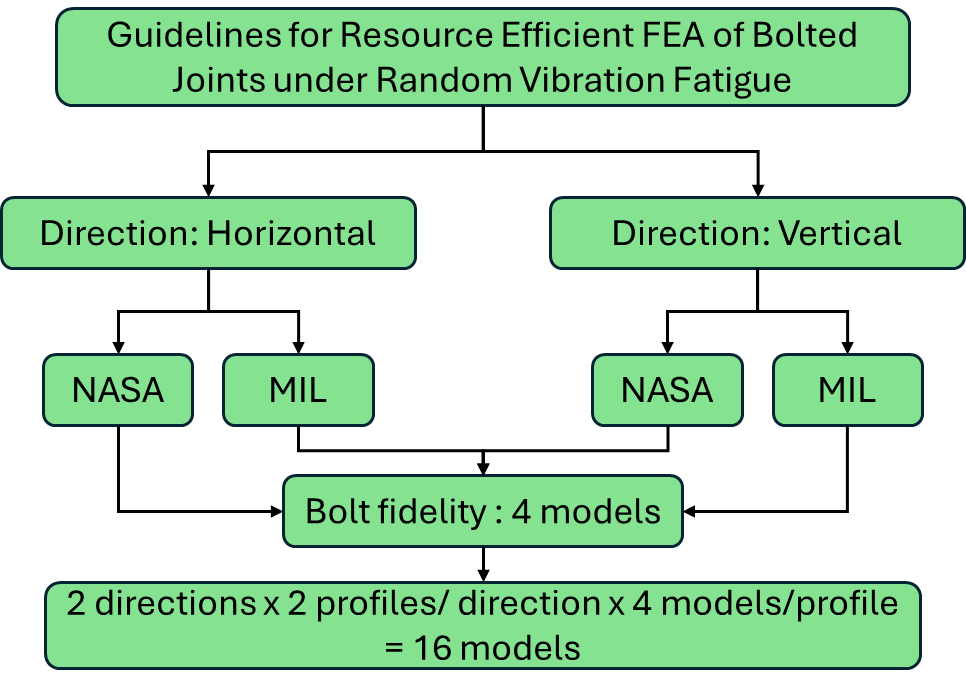
\includegraphics[width=0.96\linewidth]{Figures/researchMethod.png}
    \caption{Flowchart of the comparative computational experiment.}
    \label{fig:researchMethod}
\end{figure}

Accordingly, the thesis does not claim that the computational benchmark alone establishes the full phenomenon-method matrix. The matrix is literature-based, while the benchmark provides quantitative support for a narrower subset of modeling decisions related to stress and fatigue prediction in the present case.

\begin{itemize}
    \item Reference: The reference model is the solid bolt without threads. All further simplified models are compared against this reference for the same geometry, mesh in the clamped members, material, preload, and \ac{PSD} input.
    \item Ranking Index: Accuracy is measured nodewise in three extraction regions (clamped members, under-head fillet, first engaged thread) and combined into a single region-level score. The error combines three components: the log$_{10}$ ratio of minimum Dirlik fatigue life (weight 0.50), the relative error of the maximum \ac{RMS} von Mises stress (weight 0.30), and the relative error of 95th-percentile \ac{RMS} von Mises stress (weight 0.20), as in Equation \ref{eq:ErrorMetric}. The final Ranking Index is $ 100 e^ {-E_{combined}}$, so that perfect agreement gives $100$. Note that the Ranking Index is a ranking, it is not accuracy. It is an inversion of a sum of different errors.
    \item Cost metric: The cost of a model is the weighted sum of two solver-side quantities recorded for the same analysis step:
        \begin{enumerate}
            \item Wall-clock time to complete the analysis.
            \item Total CPU-time across all cores (core-seconds)
        \end{enumerate}
        These quantities are normalized with respect to the 3D solid reference model, so that the reference model has Cost C = 1. A simplified model that runs at 1/10 of the clock time, with proportionally reduced \ac{CPU} time, yields C = 0.1.
    \item Excluded from cost: Engineer pre-processing time, geometry preparation, mesh generation, and contact definition are excluded from the cost metric, since those are too dependent on the engineer and the pre-processing software used, rather than on the bolt representation.
    \item Efficiency Ratio: the conceptual efficiency ratio is constructed so that $\eta = 1$ for the reference model. A simplified model with $\eta > 1$ delivers more accuracy per unit cost than the reference, and a model with $\eta < 1$ does not. The efficiency ratio is computed per model, per load case, and per extraction region, so that a given model can be efficient for clamped-member fatigue while inefficient for local bolt fatigue. The conceptual efficiency ratio is defined as in Equation \ref{eq:eta}:
    \begin{equation} \label{eq:eta}
        \eta = \frac{RI}{C},
    \end{equation}
    where $RI$ is the Ranking Index and $C$ is the cost. 
\end{itemize}

Each FE modeling method is then assigned a cost, which is not objective and should be adjusted based on each guideline user's preferences. It is meant to show that model fidelity can be selected based on accuracy and cost. The guidelines should take into account specific project constraints, such as available time, required precision level, and the maturity of the input data. By following these guidelines, future projects may achieve more reliable fatigue life predictions while optimizing the use of computational engineering resources. The resulting metric should be interpreted primarily as a "ranking tool" for model selection within the studied conditions, rather than as a universal absolute measure of model adequacy.

\section{Justification of reference model} \label{sec:justification}
The comparative experiment requires a reference against which the simplified bolt models are benchmarked. Four reference candidates were considered: a physical test, a fully threaded 3D solid bolt with frictional contacts, a threadless 3D solid bolt, and an analytical solution. The 3D solid was selected.

\subsection{Why not a physical test}
Experimental validation against a measured fatigue life would link the Ranking index to physical truth rather than to a numerical model. This is the strongest form of reference and is mentioned in future work, Section \ref{chp:conclusions}, as the next step beyond the scope of this thesis. To use a physical test as the primary reference, the work would have required specimen design, fixture design, preload control, random-vibration test planning, fatigue failure monitoring, and postprocessing of measured stress or life data. This would have shifted a large portion of the project from model comparison to test development.

\subsection{Why not a fully threaded solid}
A 3D solid bolt model with threads and frictional thread contact is a good candidate to compete with physical testing. In principle, it would be the most defensible reference because it captures all the physical phenomena mentioned in this thesis and provides an adequate analysis. Two considerations ruled it out:
\begin{enumerate}
    \item The thesis used linear perturbation frequency analysis with contacts frozen at the end state of the nonlinear static preload step. To justify using the threaded model as a reference, a transient analysis would be needed. Otherwise, it would be very close to the current threadless solid.
    \item A fully threaded solid requires a much finer mesh in the thread region and more expensive contact calculations. Since the thesis compares several bolt representations across multiple excitation cases, using a fully threaded reference would have substantially increased computational cost without a proportional gain in relevance for the chosen linearized workflow.
\end{enumerate}

\newpage

\subsection{Why not an analytical solution}
There are many benefits to using an analytical solution. It is quick and easy to understand, and the analytical solution is not influenced by discretization error either. You can use it as a standard to check things like nominal member stress, preload, and joint stiffness. The analytical solution helps determine whether these things are in the correct size order.

However, an analytical solution is not sufficient as the main reference for this thesis. The central purpose of the comparison is to evaluate how different bolt representations reproduce stress-transfer behavior and fatigue-relevant response in both the clamped members and local bolt regions under random vibration. The analytical formulations available for bolted joints are typically based on simplified geometry, simplified load paths, and reduced descriptions of contact behavior. They would therefore work well for cross-validation and sanity-checking, but not as the main reference in this study for comparing model fidelity across multiple \ac{FE} representations.

\subsection{Why the threadless solid}
The threadless solid has three properties that make it defensible for the present research question:
\begin{enumerate}
    \item The model includes 3D geometry needed to model local stress transfer in the under-head region, the shank, and the engagement region. These are the regions where the other simplified models in this thesis differ most from higher-fidelity models. A reference that can solve these bearing surfaces makes those differences measurable.
    \item The threadless solid avoids some of the sensitivity that comes with thread contact, such as an increased need for local mesh convergence.
    \item In engineering practice, threadless solid bolts are commonly used when there is a need for better fidelity of information than beam, CBUSH, or bonded representations can produce. It therefore serves as a realistic reference for the practical decision problem in this thesis. Basically, it is the highest fidelity used in real life.
\end{enumerate}


\newpage
\section{Extraction from FEA}

To ensure a fair comparison, output quantities are extracted from regions that are comparable across the investigated model types whenever possible. Global or clamped-member-related response quantities can generally be compared directly between simplified and detailed models. In contrast, local bolt regions, such as under-head fillet or threads, are not equally represented across the model types. This is important for the validity of the results. A simplified model may be highly effective for one engineering question while being completely incorrect for another.

In a \ac{PSD} analysis, the stress at each node is computed from displacement mode shaped via Equation \ref{eq:sigma_BDU} ($\sigma = [B][D]\{u\}$). Each mode shape produces a single stress value per node per element, and the analysis averages across attached elements. For solid elements at shared nodes, the average and non-averaged values differ only due to mesh discretization errors, which are negligible for converged meshes.

In a multiaxial random-vibration environment, the $6\times6$ stress \ac{PSD} tensor must be reduced to a scalar equivalent, $S_{vM}(f)$, to evaluate fatigue. This is achieved using the Segalman von Mises \ac{PSD} formulation from Equation \ref{eq:SegalmanVM} in the frequency-domain, see Equation \ref{eq:SegalmanVMFreq}:

\begin{equation}\label{eq:SegalmanVMFreq}
\begin{aligned}
    S_{VM}(f) &= S_{xx}(f) + S_{yy}(f) + S_{zz}(f) - G_{xy}(f) - G_{xz}(f) - G_{yz}(f) \\& + 3S_{xyxy}(f) + 3S_{yzyz}(f) + 3S_{xzxz}(f)
\end{aligned}
\end{equation}

The equation computes the equivalent \ac{PSD} using the auto-spectral densities ($S$) and the cross-spectral densities ($G$).

Using the equivalent scalar stress \ac{PSD}, the spectral moments can be computed
\begin{equation}
    m_n = \int_0^\infty f^n S_{\mathrm{VM}}(f) df
\end{equation}

The static preload creates mean stresses that significantly impact fatigue life. The full static stress tensor is evaluated to extract the principal stresses.

Since compressive stresses generally do not drive crack initiation, unlike tensile stresses, the effective mean stress is defined as the maximum of the static stress and zero, allowing only tensile stress to be considered as the mean stress in the fatigue analysis.

For elements with a mean stress more than zero, the Goodman correction is performed using SN-curve parameters $k$ and $C$. This is done for each node.

\begin{equation} \label{eq:C_eff_Goodman}
    C_{eff} = C\cdot\left( 1- \frac{\sigma_m}{\sigma_{UTS}} \right)^k
\end{equation}

Once this is done, the fatigue damage rate $\dot{D}$ can be evaluated using the Dirlik or Steinberg method. In this thesis, Dirlik is used and compared with Steinberg in Section \ref{sec:FatigueLifeCompare}.

For large sets of elements, these computations become expensive. In this thesis, two filters were used to reduce the number of nodes computed.

The first filter in manual, setting up sets for the regions of interest. In the case of a bolted joint, regions of interest were 1) at the bolt head fillet, 2) at the first engaged thread, and 3) at the clamped members close to the bolt.

The second filter was used as a "high-pass filter", which, for each region-set, only keeps the nodes with a stress above a cut-off stress. This filtering keeps the spectral extraction focused on the nodes that contribute to fatigue, and makes the result easier to parse.

\section{Stiffness derivation for the CBUSH model} \label{sec:CBUSH_Stiffness}
The CBUSH model represents the bolted joint using a single CBUSH element with the PBUSH property, which carries six independent stiffnesses. The CBUSH captures all six \ac{DOF}s through linear springs, without solving the bolt geometry or the thread profile of the under-head contact. This makes the CBUSH representation inexpensive, but it also means that the six stiffnesses must be solved analytically before the model can be used. This section shows how the standards that are described in Chapter \ref{chp:theory} and Section \ref{sec:VDI}, \ref{sec:QFactor}, \ref{sec:DMP} can be used to solve this for an M10x1.5 joint.

The bolt axis is aligned with the element's local Z-direction, so that $K_1$ and $K_2$ correspond to the two shear directions, $K_3$ to the axial stiffness along the bolt, $K_4$ and $K_5$ to bending, and $K_6$ to torsion.

The clamped-member axial stiffness was computed using the \ac{DMP} method from Sandia SAND2008-0371. This stiffness was then combined with the VDI 2230 bolt compliance to obtain the axial CBUSH stiffness $K_3$ by

\begin{equation}
    K_3 = \left(\frac{1}{k_b}+\frac{1}{k_m}\right)^{-1}.
\end{equation}

The two shear stiffnesses, $K_1$ and $K_2$, were solved using Timoshenko beam theory. The bending stiffnesses were derived from the VDI 2230, and gave a bolt compliance of $\delta_S = 6.52 \times 10^{-7}$ rad/(N mm). The torsional stiffness was computed as $GJ/l_K$ using the polar moment of inertia of the minor-diameter circular section of the full clamping length.

Applying these four sources (Sandia, VDI 2230, Saint Venant, Timoshenko) to the M10x1.5 joint, with clamping length $l_k = 18.52$ mm, effective bearing diameter $d_{w, eff} = \min(d_w + 1.6\cdot \text{washer\_height}; d_{washer}) = 17.56$ mm, and effective Young's modulus 200 GPa for the two plates, produces the six stiffness values in Table \ref{tab:CBUSHstiffness}:

\begin{table}[H]
    \centering
    \caption{CBUSH stiffness values for the single-bolt joint studied.}
    \label{tab:CBUSHstiffness}
    \begin{tabular}{llrl}
        \toprule
        \textbf{\ac{DOF}} & \textbf{Description}       & \textbf{Value}        & \textbf{Unit} \\
        \midrule
        $K_1$        & Lateral shear, local $X$   & $1.874 \times 10^{5}$ & N/mm \\
        $K_2$        & Lateral shear, local $Y$   & $1.874 \times 10^{5}$ & N/mm \\
        $K_3$        & Axial,        local $Z$    & $3.547 \times 10^{5}$ & N/mm \\
        $K_4$        & Bending about local $X$    & $1.535 \times 10^{6}$ & N$\cdot$mm/rad \\
        $K_5$        & Bending about local $Y$    & $1.535 \times 10^{6}$ & N$\cdot$mm/rad \\
        $K_6$        & Torsion about local $Z$    & $2.168 \times 10^{6}$ & N$\cdot$mm/rad \\
        \bottomrule
    \end{tabular}
\end{table}
\newpage
The clamped member stiffnesses are $k_m = 2163.38$ kN/mm (DMP), $1034.76$ kN/mm (Bickford Q-factor), and $2711.06$ kN/mm (VDI cone). The Bickford value is approximately half the DMP value, with a ratio DMP/Bickford $= 2.09$.

For the present joint, the DMP-based load factor is $\Phi = 0.1409$, the VDI cone gives $\Phi = 0.1157$, and the Bickford Q-factor gives $\Phi = 0.2553$. The DMP and VDI agree within approximately 22 \% while the Q factor is off by 180 - 200 \%.

\section{Validity and reliability of the approach} \label{sec:validity}

The computational experiment in this thesis is designed to isolate the effect of bolt modeling fidelity on fatigue life prediction while keeping all other variables constant. The same geometry, material properties, mesh density, boundary conditions, and \ac{PSD} inputs are used across all four modeling strategies. This controlled setup increases validity because observed differences can be assumed to be because of the bolt representation, rather than other factors.

Three measures are taken to increase the reliability of the results:
\begin{enumerate}
    \item The modal analysis results (eigen frequencies and mode shapes) are compared across all methods to identify at which modes the simplified representations diverge from the "truth". 
    \item The mesh in the clamped members is kept identical across all methods to ensure that any differences in the stress \ac{PSD} are due solely to the bolt model.
    \item The free-free dynamic response is compared to the origin of the geometry in \cite{27}, confirming that the reproduction of the published benchmark is consistent with its reported modal behavior before the comparative study, in Figure \ref{fig:modal27}:
\end{enumerate}

\begin{figure}[H]
    \centering
    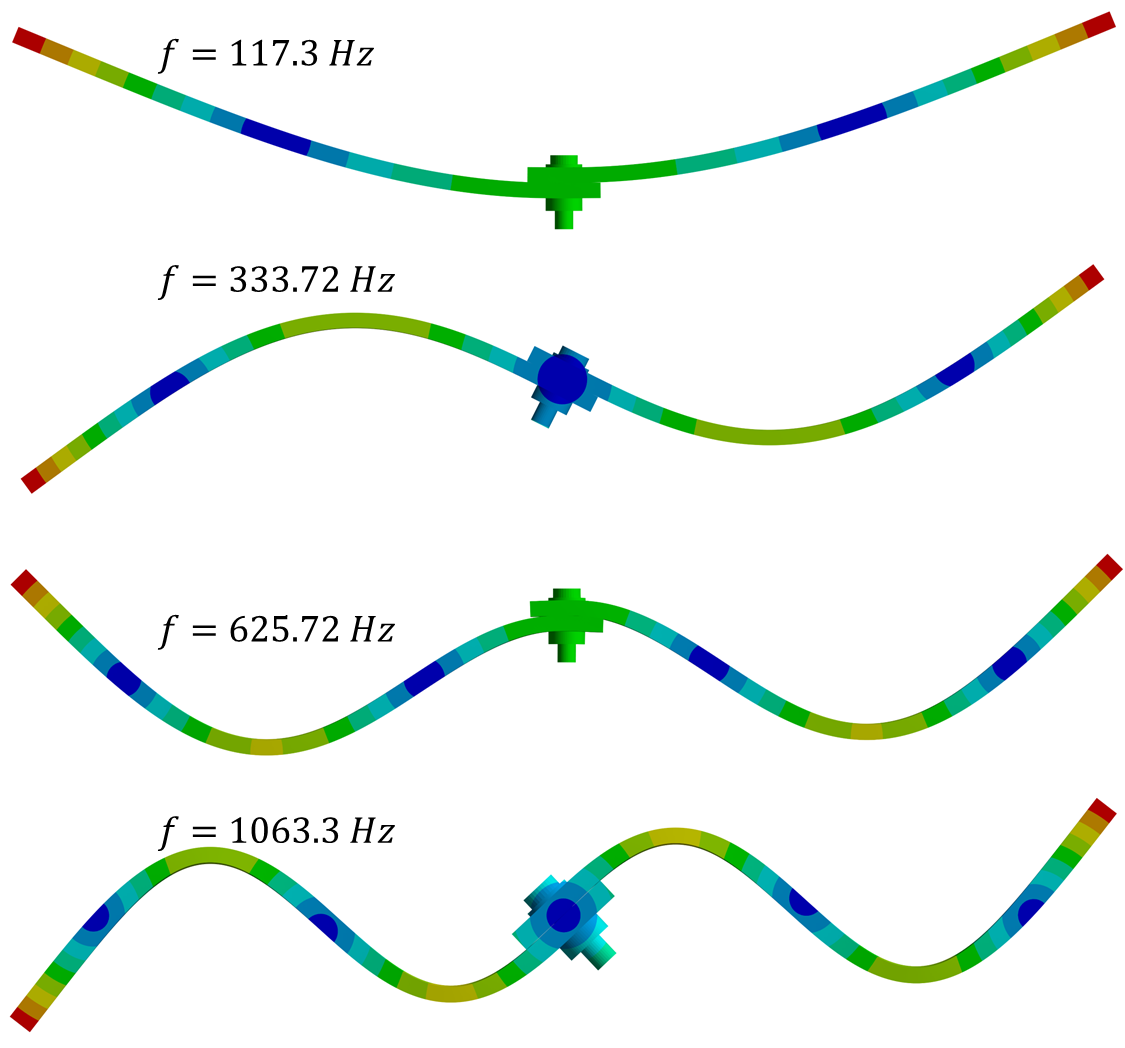
\includegraphics[width=0.65\linewidth]{Figures/MODAL27.png}
    \caption{Free-free mode shapes from this simulation. The first three shapes are compared with the source of the geometry.}
    \label{fig:modal27}
\end{figure}

The free-free modal shapes and eigen frequencies match the experimental data that Kim \textit{et al.} \cite{27} obtained, and the comparison of the first four bending modes eigen frequencies can be seen in Table \ref{tab:compareEigen}, where the difference is computed as $100 (this-kim)/kim$:

\begin{table}[H]
    \centering
    \caption{Eigen frequency comparison simulation vs experiment}
    \label{tab:compareEigen}
    \begin{tabular}{lccc}
        \toprule
        & \textbf{This thesis} & \textbf{Kim \textit{et al.}} & \textbf{Difference [\%]} \\
        \midrule
        Mode 1 & 117.3 Hz  & 120 Hz  & -2.25       \\
        Mode 2 & 333.72 Hz & 332 Hz  & +0.52 \\
        Mode 3 & 625.72 Hz & 640 Hz  & -2.23    \\
        Mode 4 & 1063.3 Hz & 1060 Hz & +0.31 \\
        \bottomrule
    \end{tabular}
\end{table}

A limitation of the approach is that the linear perturbation method freezes the contact state at the end of the static preload step. This means that contact-status-dependent phenomena that would normally occur during the dynamic loading, such as contact opening, micro-slip, and amplitude-dependent damping, are not captured. For the excitation levels considered in this thesis, this is an acceptable approximation. Still, for higher-amplitude loads where the joint may undergo macro-slip, a fully nonlinear transient analysis would be required, as noted in Section \ref{sec:experimental}. The geometry that is used is directly from Kim \textit{et al.}, and can be seen in Figure \ref{fig:Drawing1}:
\begin{figure}[H]
    \centering
    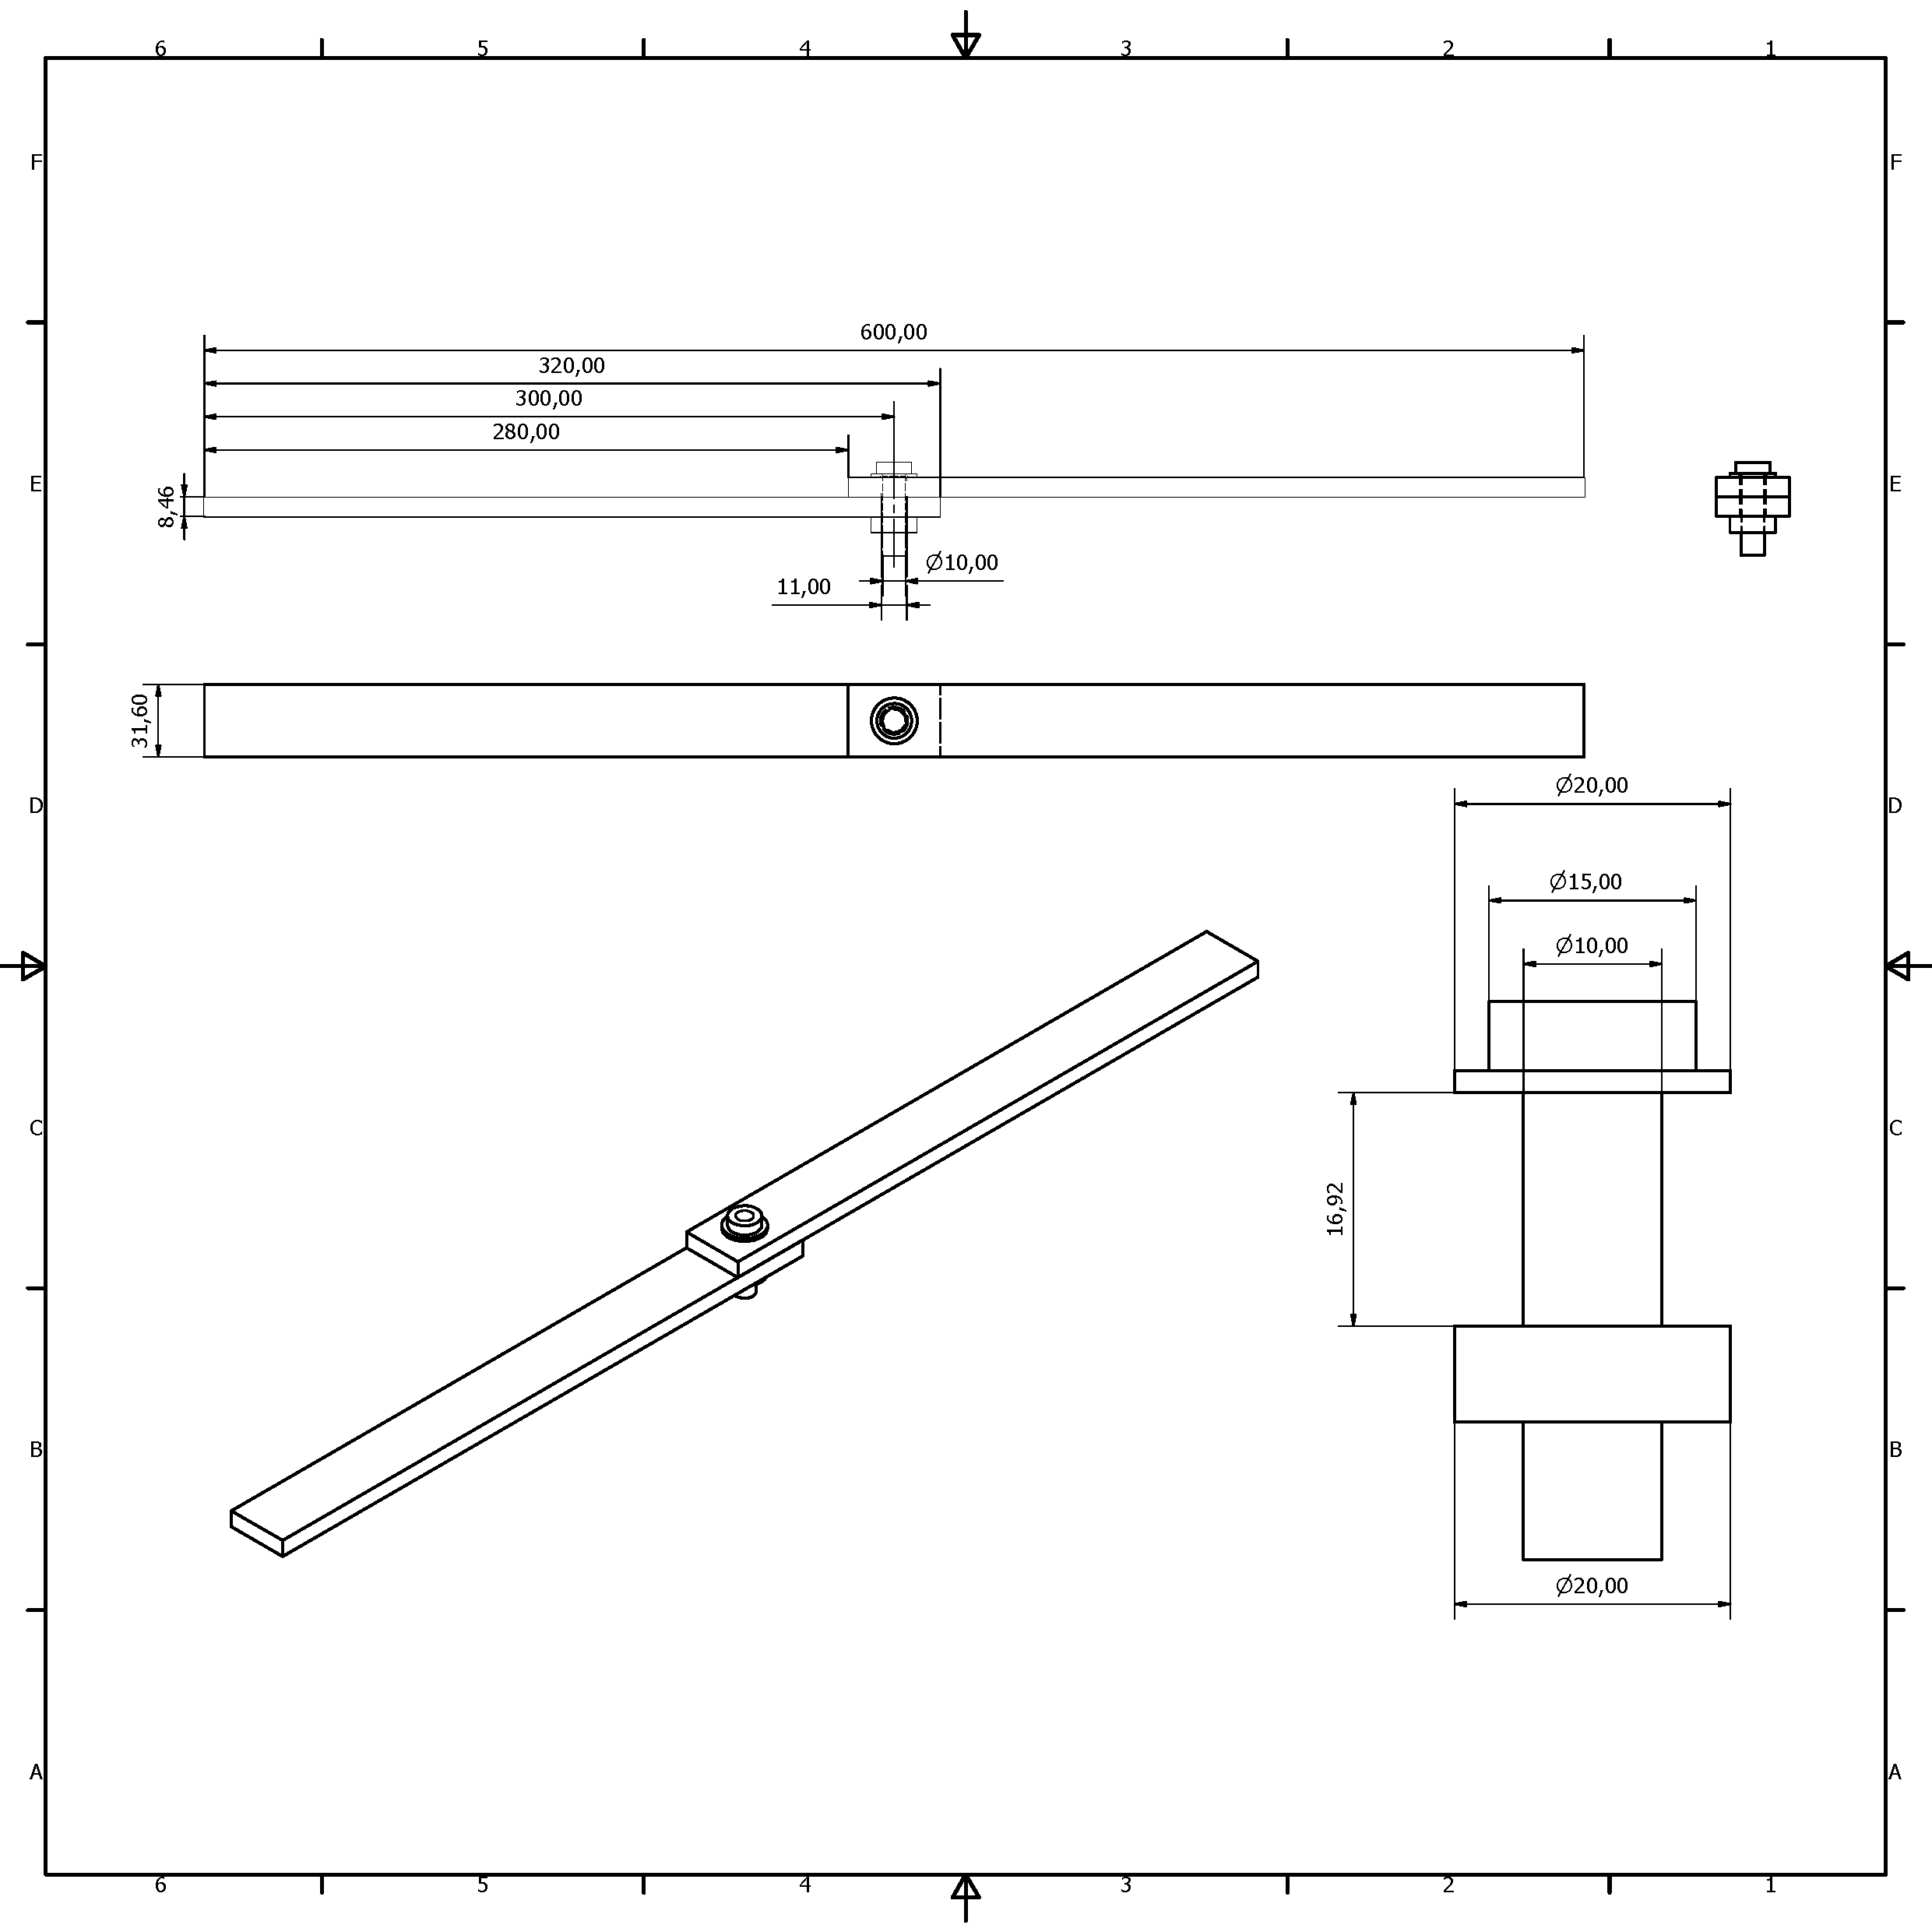
\includegraphics[width=0.75\linewidth]{27 Assembly.pdf}
    \caption{The geometry benchmark that is used in this thesis.}
    \label{fig:Drawing1}
\end{figure}

The geometry is then excited as in Figure \ref{fig:excitationDrawing}:

\begin{figure}[H]
    \centering
    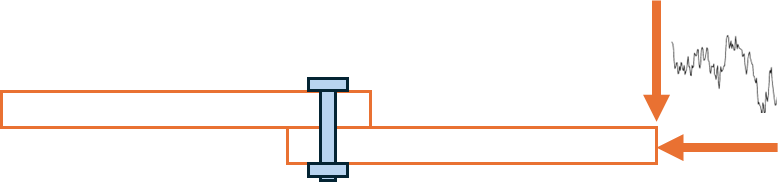
\includegraphics[width=0.75\linewidth]{Figures/excitationDrawing.png}
    \caption{Drawing of the excitations. Note that only one direction is excited at a time, not simultaneously.}
    \label{fig:excitationDrawing}
\end{figure}

\subsection{Analytical cross-validations}

To increase the validity of the numerical results, some cross-validation is performed.

First, using Equation \ref{eq:TensileStressArea} we get
\begin{equation}
    A_s = \frac{\pi}{4} \left( \frac{d_2 + d_3}{2} \right)^2 = \frac{\pi}{4} \left( \frac{9.026 + 8.16}{2} \right)^2 = 57.99 mm^2,
\end{equation}
which is compliant with the handbooks or standards such as the SS-EN-ISO-898-1-2013, where $A_s$ for M10 bolts are specified to be $58$ mm$^2$ \cite{SSENISO898-1-2013}.

The main shaft's stress is 495.86 MPa. The bolt shank has a diameter of 10 mm through the hole length, which means that it has a cross-sectional area of $\tfrac{\pi}{4} \cdot 10^2 = 78.54$ mm$^2$, but that's not the smallest area on the real bolt, which would be $A_S = 58$ mm$^2$. Therefore, to validate that number, we would need to compute

\begin{equation}
    \begin{aligned}
        F &= \sigma_{sim}A_{sim} = \sigma_{real}A_{S} \\
        &\rightarrow \sigma_{real} = \frac{A_{sim}}{A_S} \sigma_{sim} = \frac{78.54}{58.00}\cdot 495.86 MPa = 671.46 MPa,
    \end{aligned}
\end{equation}
which align well with the expected $\sigma_m = 0.7\cdot 940 MPa = 658.00$ MPa.

At the underhead fillet, the simulation shows a local stress of 1022.50 MPa during the nonlinear static preload step. A simple analytical comparison can be made by multiplying the nominal shank stress by an estimated stress concentration factor. Using $k_t = 2.3$ for this region from Section \ref{sec:SCF}, an analytical estimate of this stress would be

\begin{equation}
    k_t \cdot \sigma_{sim} = 2.3 \cdot \tfrac{F_M}{A_{sim}} = 2.3\tfrac{38164 N}{78.54 mm^2} = 1118 MPa.
\end{equation}

The simulated value is $\tfrac{1022.50 - 1118}{1118} = -8.54$ \% lower than the analytical estimate, which might be acceptable since Shigley does not specify a certain head-fillet radius, so there is some uncertainty. Both 1118 MPa (analytical) and 1022.5 MPa (simulated) are linear-elastic peak stresses. They exceed the nominal yield strength $R_{p0.2} = 940$ MPa of class 10.9 steel, and the analytical estimate exceeds the ultimate strength $\sigma_u = 1040$ MPa. In a real bolt, local plasticity would redistribute the stress peaks, capping the stress near $R_{p0.2}$. The linear-elastic model used here cannot represent this redistribution and therefore overestimates the local peak. The agreement between the analytical and simulated values shows that the model is internally consistent in the linear-elastic context, but it does not validate the absolute stress level. 


The bolt model has no threads, so comparing the local stress to the expected stress at the first engaged thread is not meaningful. However, the stress concentration according to Shigley for cut threads is 3.8, so the analytically expected stress would be $3.8\cdot 658 = 2500.4$ MPa, which is more than twice the ultimate strength of class 10.9 steel. This value is, however, not what the bolt would actually experience. The factor $K_t$ is an elastic geometric \ac{SCF} and assumes that the material remains linear-elastic. In a real bolt, the highly stressed material at the first engaged thread yields locally during tightening. The elastic peak stress is a useful indication that the local thread-root stress is beyond the linear-elastic context, but does not imply that the bolt would fail under the intended preload.

\begin{figure}[H]
    \centering
    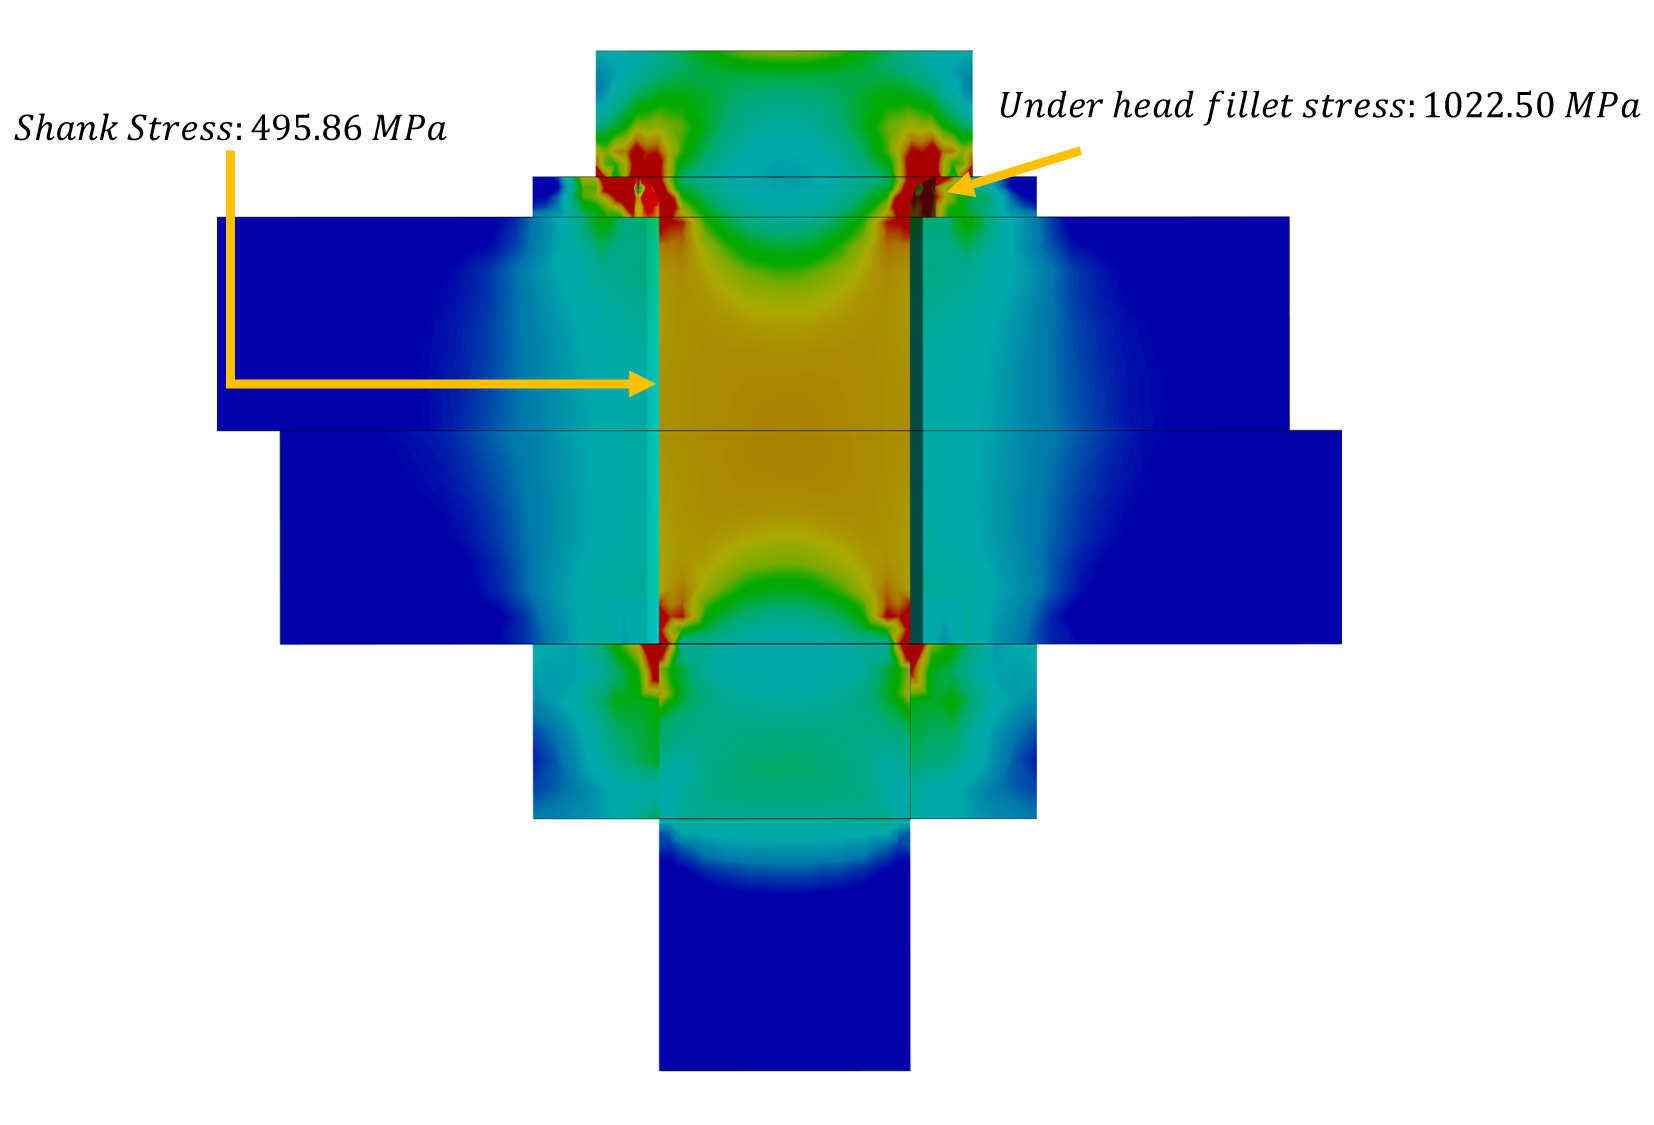
\includegraphics[width=0.72\linewidth]{Figures/stressSimValidation.png}
    \caption{Measured stresses from the nonlinear static preload step.}
    \label{fig:stressSimValidation}
\end{figure}

\subsection{Cross-Validation between Stiffness standards}
For the specific geometry in this thesis, with one M10 bolt and two steel plates (material is discussed in the limitations Section \ref{sec:limitations}), $l_k = 18.52$ mm, the stiffnesses are evaluated from the standards in Table \ref{tab:StandardCompare}, with errors defined as $\tfrac{method - DMP}{DMP}$:

\begin{table}[H]
    \centering
    \caption{Comparison of the values from the Standards}
    \label{tab:StandardCompare}
    \begin{tabular}{lccccc}
        \toprule
        Method & $k_m$ [N/mm] & Load factor [] & $E_{stiffness}$ [\%] & $E_{Load\, factor}$ [\%] \\
        \midrule
        Sandia DMP & 2163.38 & 0.1409 & 0 & 0 \\
        VDI 2230 & 2711.06 & 0.1157 & 25.316 & -17.885 \\
        Sandia Bickford Q-factor & 1034.76 & 0.2553 & -52.169 & 81.192 \\
        \bottomrule
    \end{tabular}
\end{table}

The comparison shows that the analytical stiffness estimate is sensitive to the selected clamped-member model. For the current geometry, the VDI cone model yields a higher clamped-member stiffness than the DMP method, whereas the Bickford Q-factor method yields a lower stiffness. These differences should not be interpreted as direct errors, since no experimental stiffness measurement is used as the reference in this comparison. Instead, the table illustrates the uncertainty introduced by the analytical stiffness model itself.

\subsection{Defending the choice of excitation PSDs}

To determine which \ac{PSD} to apply to the assembly, two standard test documents were evaluated, and two excitation \ac{PSD}s were selected to represent two relevant standardized random-vibration environments: a spacecraft workmanship environment and an aircraft transport environment, shown in Figure \ref{fig:ChosenPSDs}. The purpose is to compare different modeling strategies using realistic, widely used broadband vibration inputs. Their use enhances the study's practical relevance, but the conclusions must be interpreted within the range of the selected load cases. The results, therefore, support the development of guidelines for the investigated excitations but do not establish universal validity across all possible random vibration environments.

\begin{figure}[H]
    \centering
    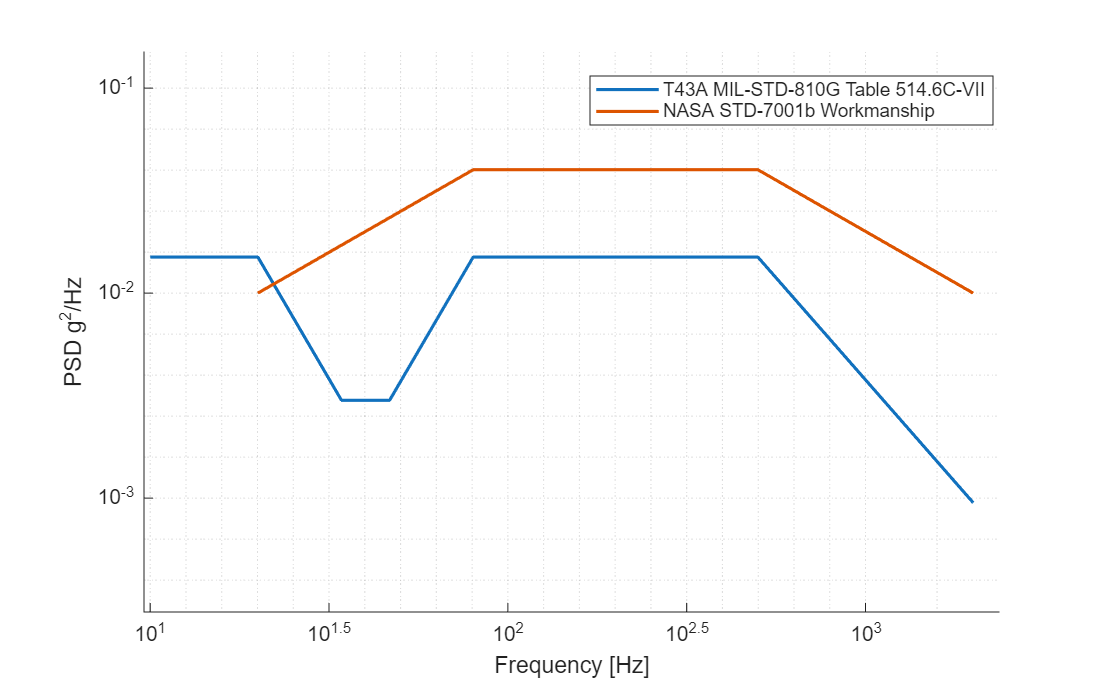
\includegraphics[width=0.75\linewidth]{Figures/PSD's5.png}
    \caption{The chosen PSD curves.}
    \label{fig:ChosenPSDs}
\end{figure}



The NASA-STD-7001B Workmanship \ac{PSD} was chosen because it defines a minimum random-vibration level for spaceflight payload components. It is intended to reveal workmanship defects and manufacturing flaws in electronic and electromechanical hardware. For components below 50 kg, the spectrum covers 20-2000 Hz, with a plateau of 0.04 $g^2/Hz$ between 80 and 500 Hz, yielding an overall level of 6.8 $g_{RMS}$, where $g_{rms}$ is the root-mean-square acceleration expressed in multiples of $g$ (the square root of the area under the acceleration \ac{PSD}). This makes it a suitable reference case for evaluating how the different bolt representations respond to a relatively severe spacecraft-related vibration input. 

The MIL-STD-810G T43A \ac{PSD} was selected as a second load case because it represents jet-transport cargo vibration. In Method 514.6, Category 7 in the standard, the jet-aircraft cargo environment is described as broadband random vibration, with the highest levels occurring during take-off. The T43A curve is therefore relevant for equipment or payload hardware that may be transported by aircraft. The T43A spectrum has an overall level of 3.54 $g_{RMS}$, with defined breakpoints between 10 and 2000 Hz.

Using both \ac{PSD}s gives two distinct excitation cases with different severity and spectral content. This allows indicating whether the relative accuracy of the bolt representations is robust to the chosen vibration environment, rather than being valid only for a specific \ac{PSD} shape.


\section{Mesh convergence}
Two mesh convergence tests were performed: one for the nonlinear static preload step and one for the frequency response used in the fatigue calculation. These are different convergence problems, and a mesh that converges for one does not automatically converge for the other. In this thesis, three quantities are used in the fatigue life:
\begin{enumerate}
    \item Stress \ac{PSD} in critical regions (under-head fillet, first engaged thread, clamped members)
    \item \ac{RMS} stress (area integral of the \ac{PSD})
    \item Minimum Dirlik fatigue life (nonlinear function of \ac{PSD} shape)
\end{enumerate}

The mesh convergence study is found in Appendix \ref{app:MeshConvergence}.

\section{Ranking index}

The index introduced below is an illustrative engineering comparison aid, designed to \textit{feel} like accuracy for the present benchmark. It combines relative errors in fatigue life and \ac{RMS} stress with computational time to visualize the trade-off between response accuracy and solution cost for the studied models. The index is not an absolute measure of model validity. It should therefore be interpreted only within the context of the geometry, loading conditions, response quantities, and reference model used in this study.

The main conclusions of the thesis do not depend solely on this index - they are instead based on comparisons of stress and fatigue responses.

The Ranking Index is meant to quantify agreement between models. It is computed for each region and model combination based on a weighted combination of fatigue-life-ratio error and RMS-stress relative error. The purpose of the Ranking Index is not to replace engineering judgment but to summarize how closely each simplified model approximates the solid reference in regions where a meaningful comparison is possible.

The proposed Ranking Index combines three quantities: the minimum Dirlik fatigue life, the maximum \ac{RMS} stress, and the 95th percentile \ac{RMS} stress. The life term is given the highest weight because fatigue life is the most design-relevant output. In contrast, the RMS-based terms are included to capture both peak response and the broader stress distribution within the region. 
The weights (0.50 for fatigue life, 0.30 for maximum RMS, 0.20 for 95th-percentile RMS) reflect the engineering prioritization in this thesis: fatigue life dominates the design decision because it is the directly design-relevant output. At the same time, the \ac{RMS} terms capture peak response and broader stress distribution. The ranking index is a deliberately constructed engineering aid rather than a derived measure of accuracy. The weights are defensible defaults for the present application: fatigue failure is the dominant failure mode for bolted joints under cyclic loading, so it is weighted most heavily, with RMS-stress terms capturing peak and bulk responses as secondary checks. The weights should be adjusted to reflect the engineering question of the specific application. The sensitivity of the model ranking to these weights is examined in Section \ref{sec:Tornado}.

The combined error is defined according to Equation \ref{eq:ErrorMetric}:

\begin{equation} \label{eq:ErrorMetric}
    E_{combined} = 0.50E_{life} + 0.30 E_{max\, RMS} + 0.20E_{95\, RMS}
\end{equation}

where the life error is measured on a logarithmic scale
\begin{equation} \label{eq:Elife}
    E_{life} = \left| log_{10}\left( \frac{T_{model}}{T_{truth}} \right) \right|
\end{equation}

and the \ac{RMS} terms are expressed as relative deviations

\begin{equation} \label{eq:EMaxRMS}
     E_{max\, RMS} = \left| \frac{\sigma_{RMS\, max \, , model} - \sigma_{RMS\, max \, , truth}}{\sigma_{RMS\, max \, , truth}} \right|,
\end{equation}

\begin{equation} \label{eq:E95RMS}
    E_{95\, RMS} = \left| \frac{\sigma_{RMS\, 95 \, , model} - \sigma_{RMS\, 95 \, , truth}}{\sigma_{RMS\, 95 \, , truth}} \right|.
\end{equation}

The final Ranking Index $RI$ is then defined as
\begin{equation} \label{eq:AccuracyMetric}
    RI = 100e^{-E_{combined}},
\end{equation}

so that a perfect match gives a score of 100, and increasing error causes the score to decrease smoothly. The results of this are found in Appendix \ref{app:RI_tables}.



\section{Cost metric} \label{sec:costMetric}
The four bolt representations were solved on the same hardware and solver configuration. Wall-clock and CPU seconds were recorded from the output and are listed in Table \ref{tab:WC_CPU}, where subscript $n$ means normalized against the threadless 3D solid reference, and the normalized cost $C$ used in the Efficiency Ratio (Equation \ref{eq:eta}) is the arithmetic mean of the two normalized columns. Every normalized metric $(\cdot)_n$ for representation $i$ is computed according to Equation \ref{eq:Normalized} and \ref{eq:CostFunction}:

\begin{equation} \label{eq:Normalized}
    \begin{aligned}
        WC_{n, i} &= \frac{WC_i}{WC_{ref}}\\
        CPU_{n, i} &= \frac{CPU_i}{CPU_{ref}}\\
    \end{aligned}
\end{equation}

\begin{equation} \label{eq:CostFunction}
    C_{n, i} = 100\frac{WC_{n, i}+CPU_{n, i}}{2}
\end{equation}

All simulations were solved on the same workstation to ensure that the cost values are directly comparable. The hardware and solver configuration were: Intel Core Ultra 9 285HX, 2.80 GHz base speed, 24 cores / 24 logical processors, 64 GB RAM installed, solver OptiStruct 2024.1 running on Windows 11. Each analysis was restricted to the 8 performance cores only. No other heavy processes were active during the runs.

\chapter{Results and Analysis}
\label{chp:results}

This chapter presents the results of the model comparison and uses them to develop practical engineering guidelines for \ac{FEA} of bolted joints under random vibration, with respect to fatigue. The analysis focuses on how model fidelity influences predicted response, fatigue-related metrics, and computational efficiency.

The guidelines presented in this chapter are built on two different evidence bases and should be interpreted accordingly. First, the phenomenon-method matrix is a literature- and theory-derived capability map. Its function is to indicate which \ac{FE} representation and analysis type is generally required to capture a given physical phenomenon at a useful engineering level. Second, the comparative simulation results in this chapter provide quantitative benchmark evidence for the stress- and fatigue-related performance of the studied bolt models in the present single-bolt configuration. The matrix should therefore be read as a qualitative capability map, while the computational results should be read as quantitative evidence for the narrower benchmark problem studied here.

\section{Stress PSD comparison}
Figure \ref{fig:Stress_PSD_Members_Comparison}, \ref{fig:Stress_PSD_UnderHead_Comparison}, and \ref{fig:Stress_PSD_AtNut_Comparison} show the von Mises equivalent stress \ac{PSD} $S_{VM}(f)$ for the five most critical nodes per model in each of the three extraction regions, presented side by side for transverse and axial loading. The extraction regions are the clamped members, the bolt under-head fillet, and the bolt at the nut bearing surface. The side-by-side comparison makes it easier to check whether the same trends hold across loading directions.

\subsection{Clamped Members}

In the clamped members (Figure \ref{fig:Stress_PSD_Members_Comparison}), the solid and the beam models produce stress PSDs of comparable shape and magnitude under both loading directions, with resonant peaks aligned at the same modal frequencies. The bonded representation places its resonant peaks at the same modal frequencies but with \ac{PSD} amplitudes roughly half an order of magnitude higher. This is consistent with the modeling assumption behind a fully bonded contact: bonded contacts "glue" the contacting surfaces with no possibility of separation or slip. The joint, therefore, behaves locally as a perfectly welded region, which is stiffer than the actual frictional bolted joint and excites larger response amplitudes at resonance. The same effect was observed experimentally on the Brake-Reuß beam by Lacayo \textit{et al.}, where bonded representation overestimates the natural frequency relative to the calibrated nonlinear joint and misses the amplitude-dependent damping \cite{15}.
The CBUSH model falls between the beam and bonded models.

Under axial loading, the absolute \ac{PSD} amplitudes are approximately one order of magnitude higher than under transverse loading. Despite this shift, the relative rankings of the models remain unchanged: the beam model closely tracks the solid reference, while the bonded and CBUSH models overshoot.

\begin{figure}[H]
    \centering
    \begin{subfigure}[b]{0.45\textwidth}
        \centering
        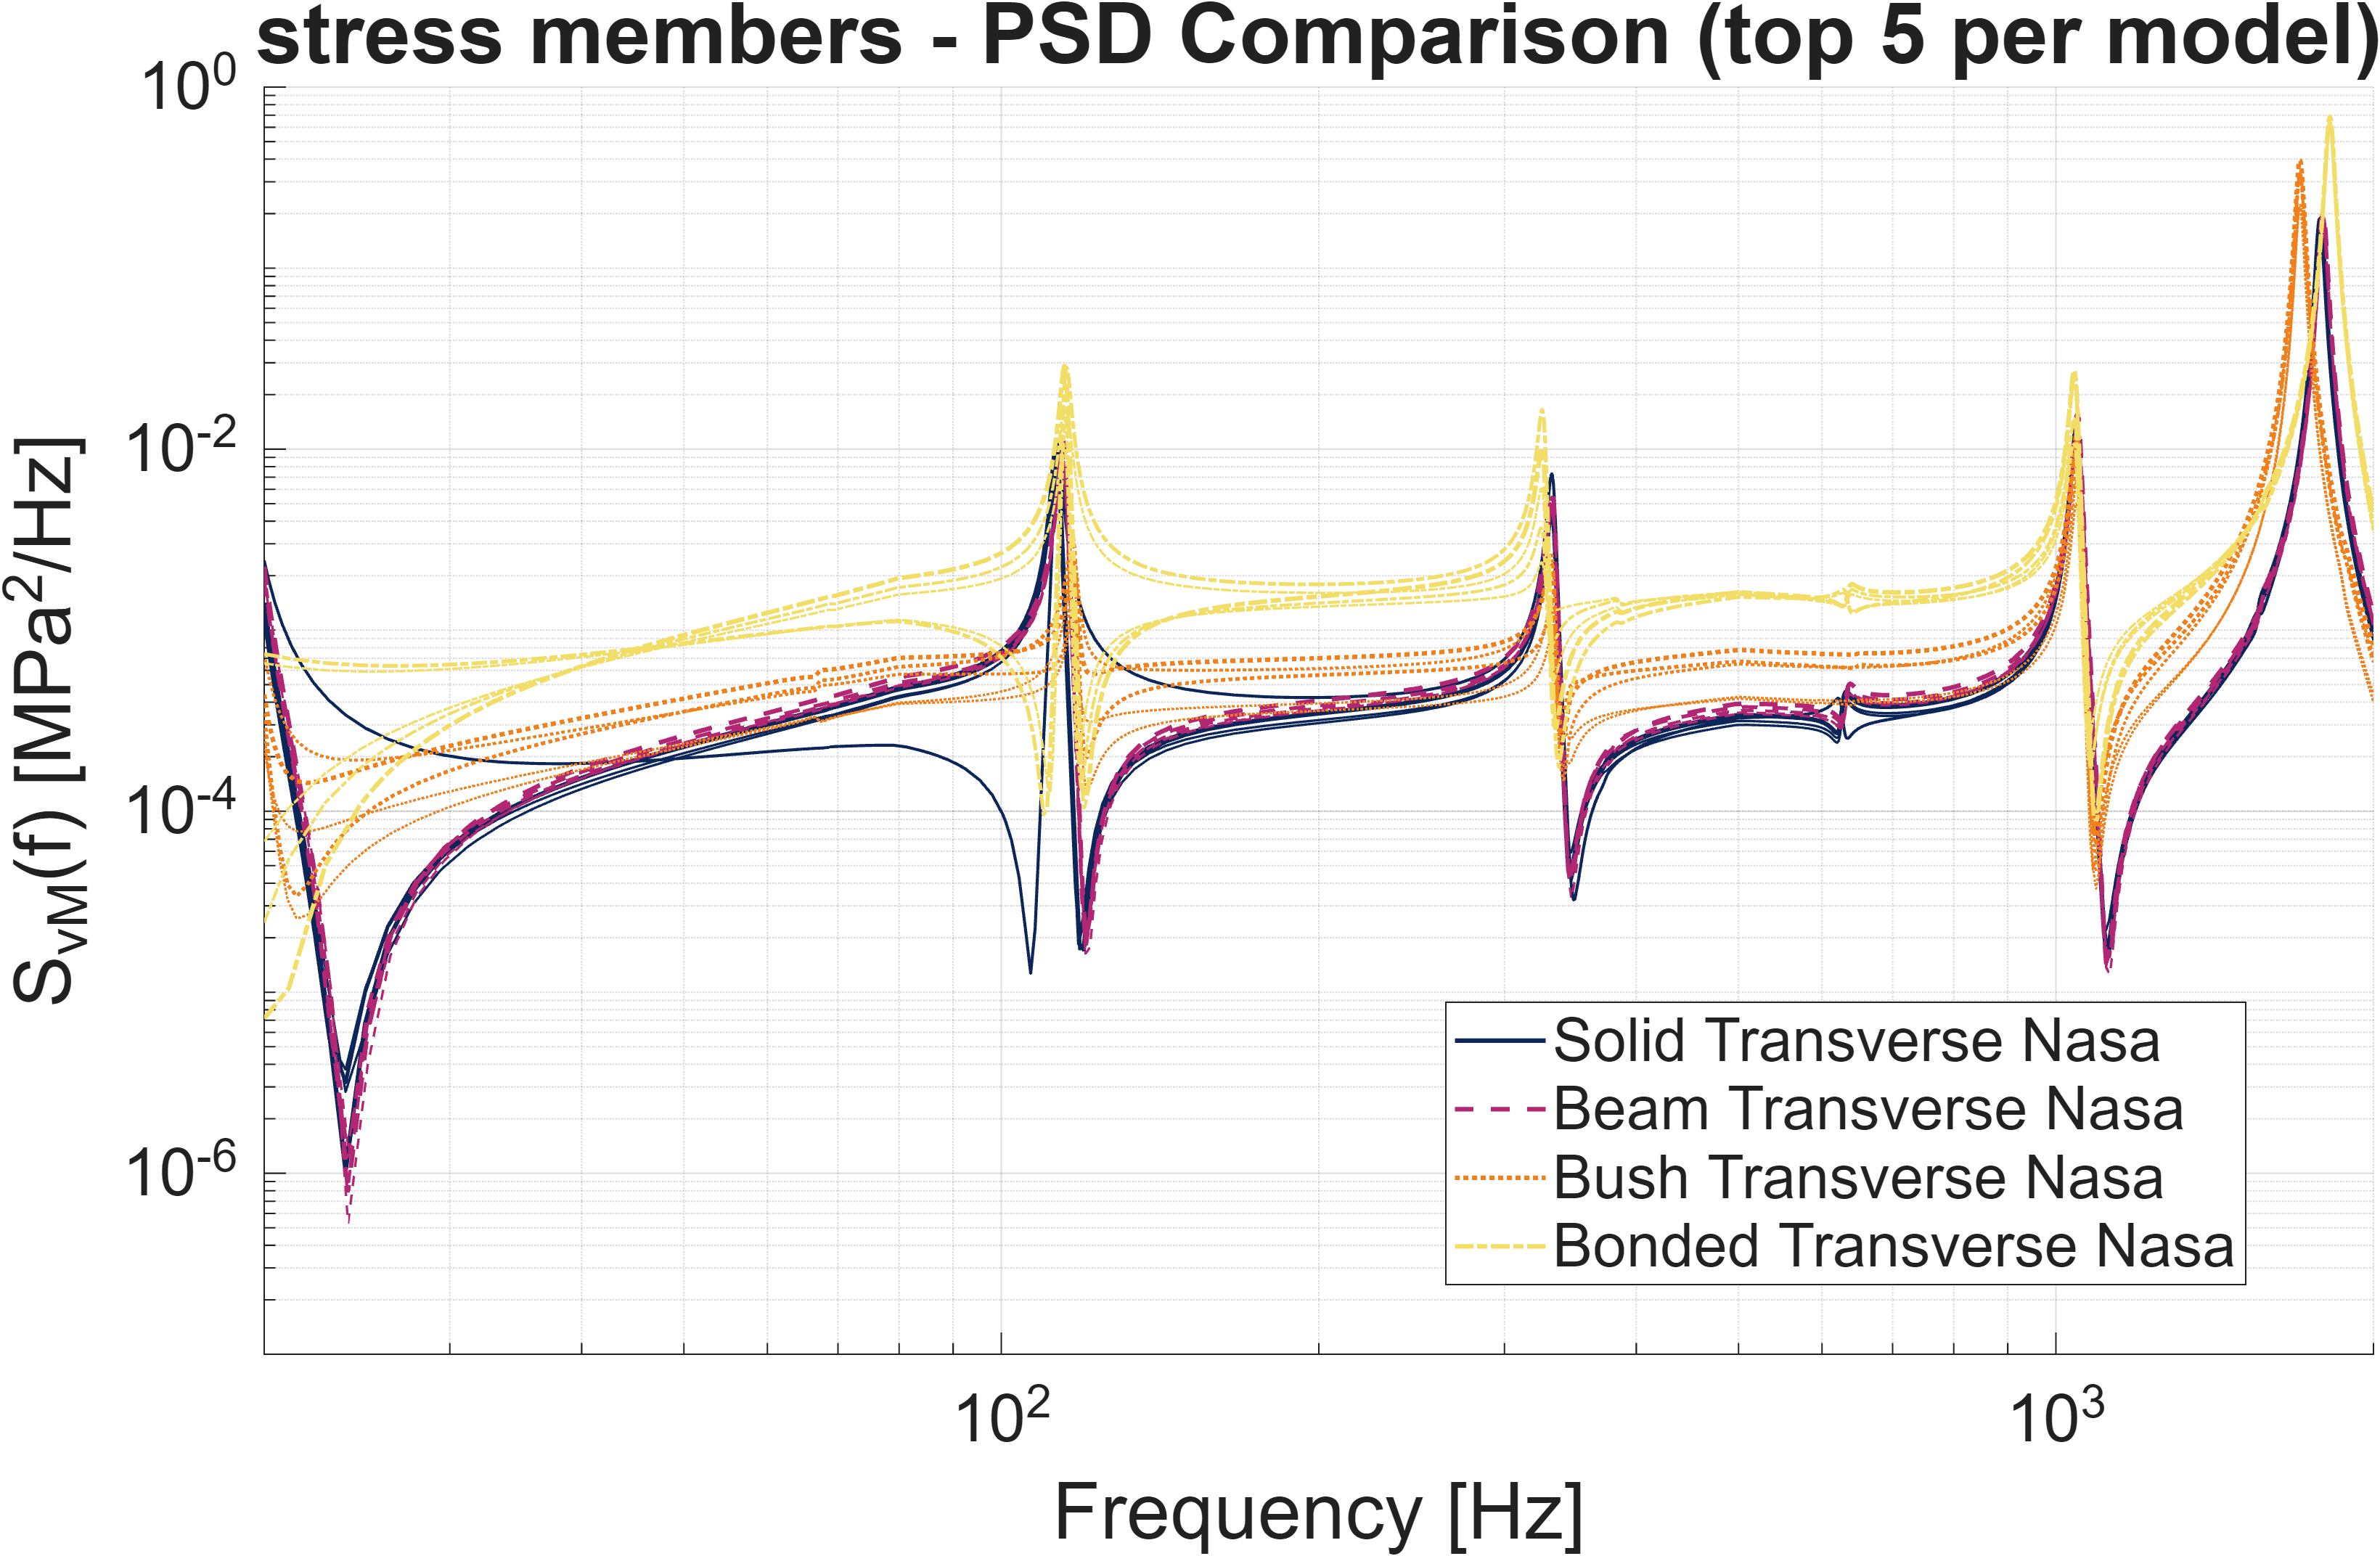
\includegraphics[width=\textwidth]{Transverse Nasa/Transverse Nasa_psd_overlay_NODEWISE stress_members.png}
        \caption{Transverse Loading (shear).}
        \label{fig:NASA_shear_psd_overlay_NODEWISE_stress_members}
    \end{subfigure}
    \begin{subfigure}[b]{0.45\textwidth}
        \centering
        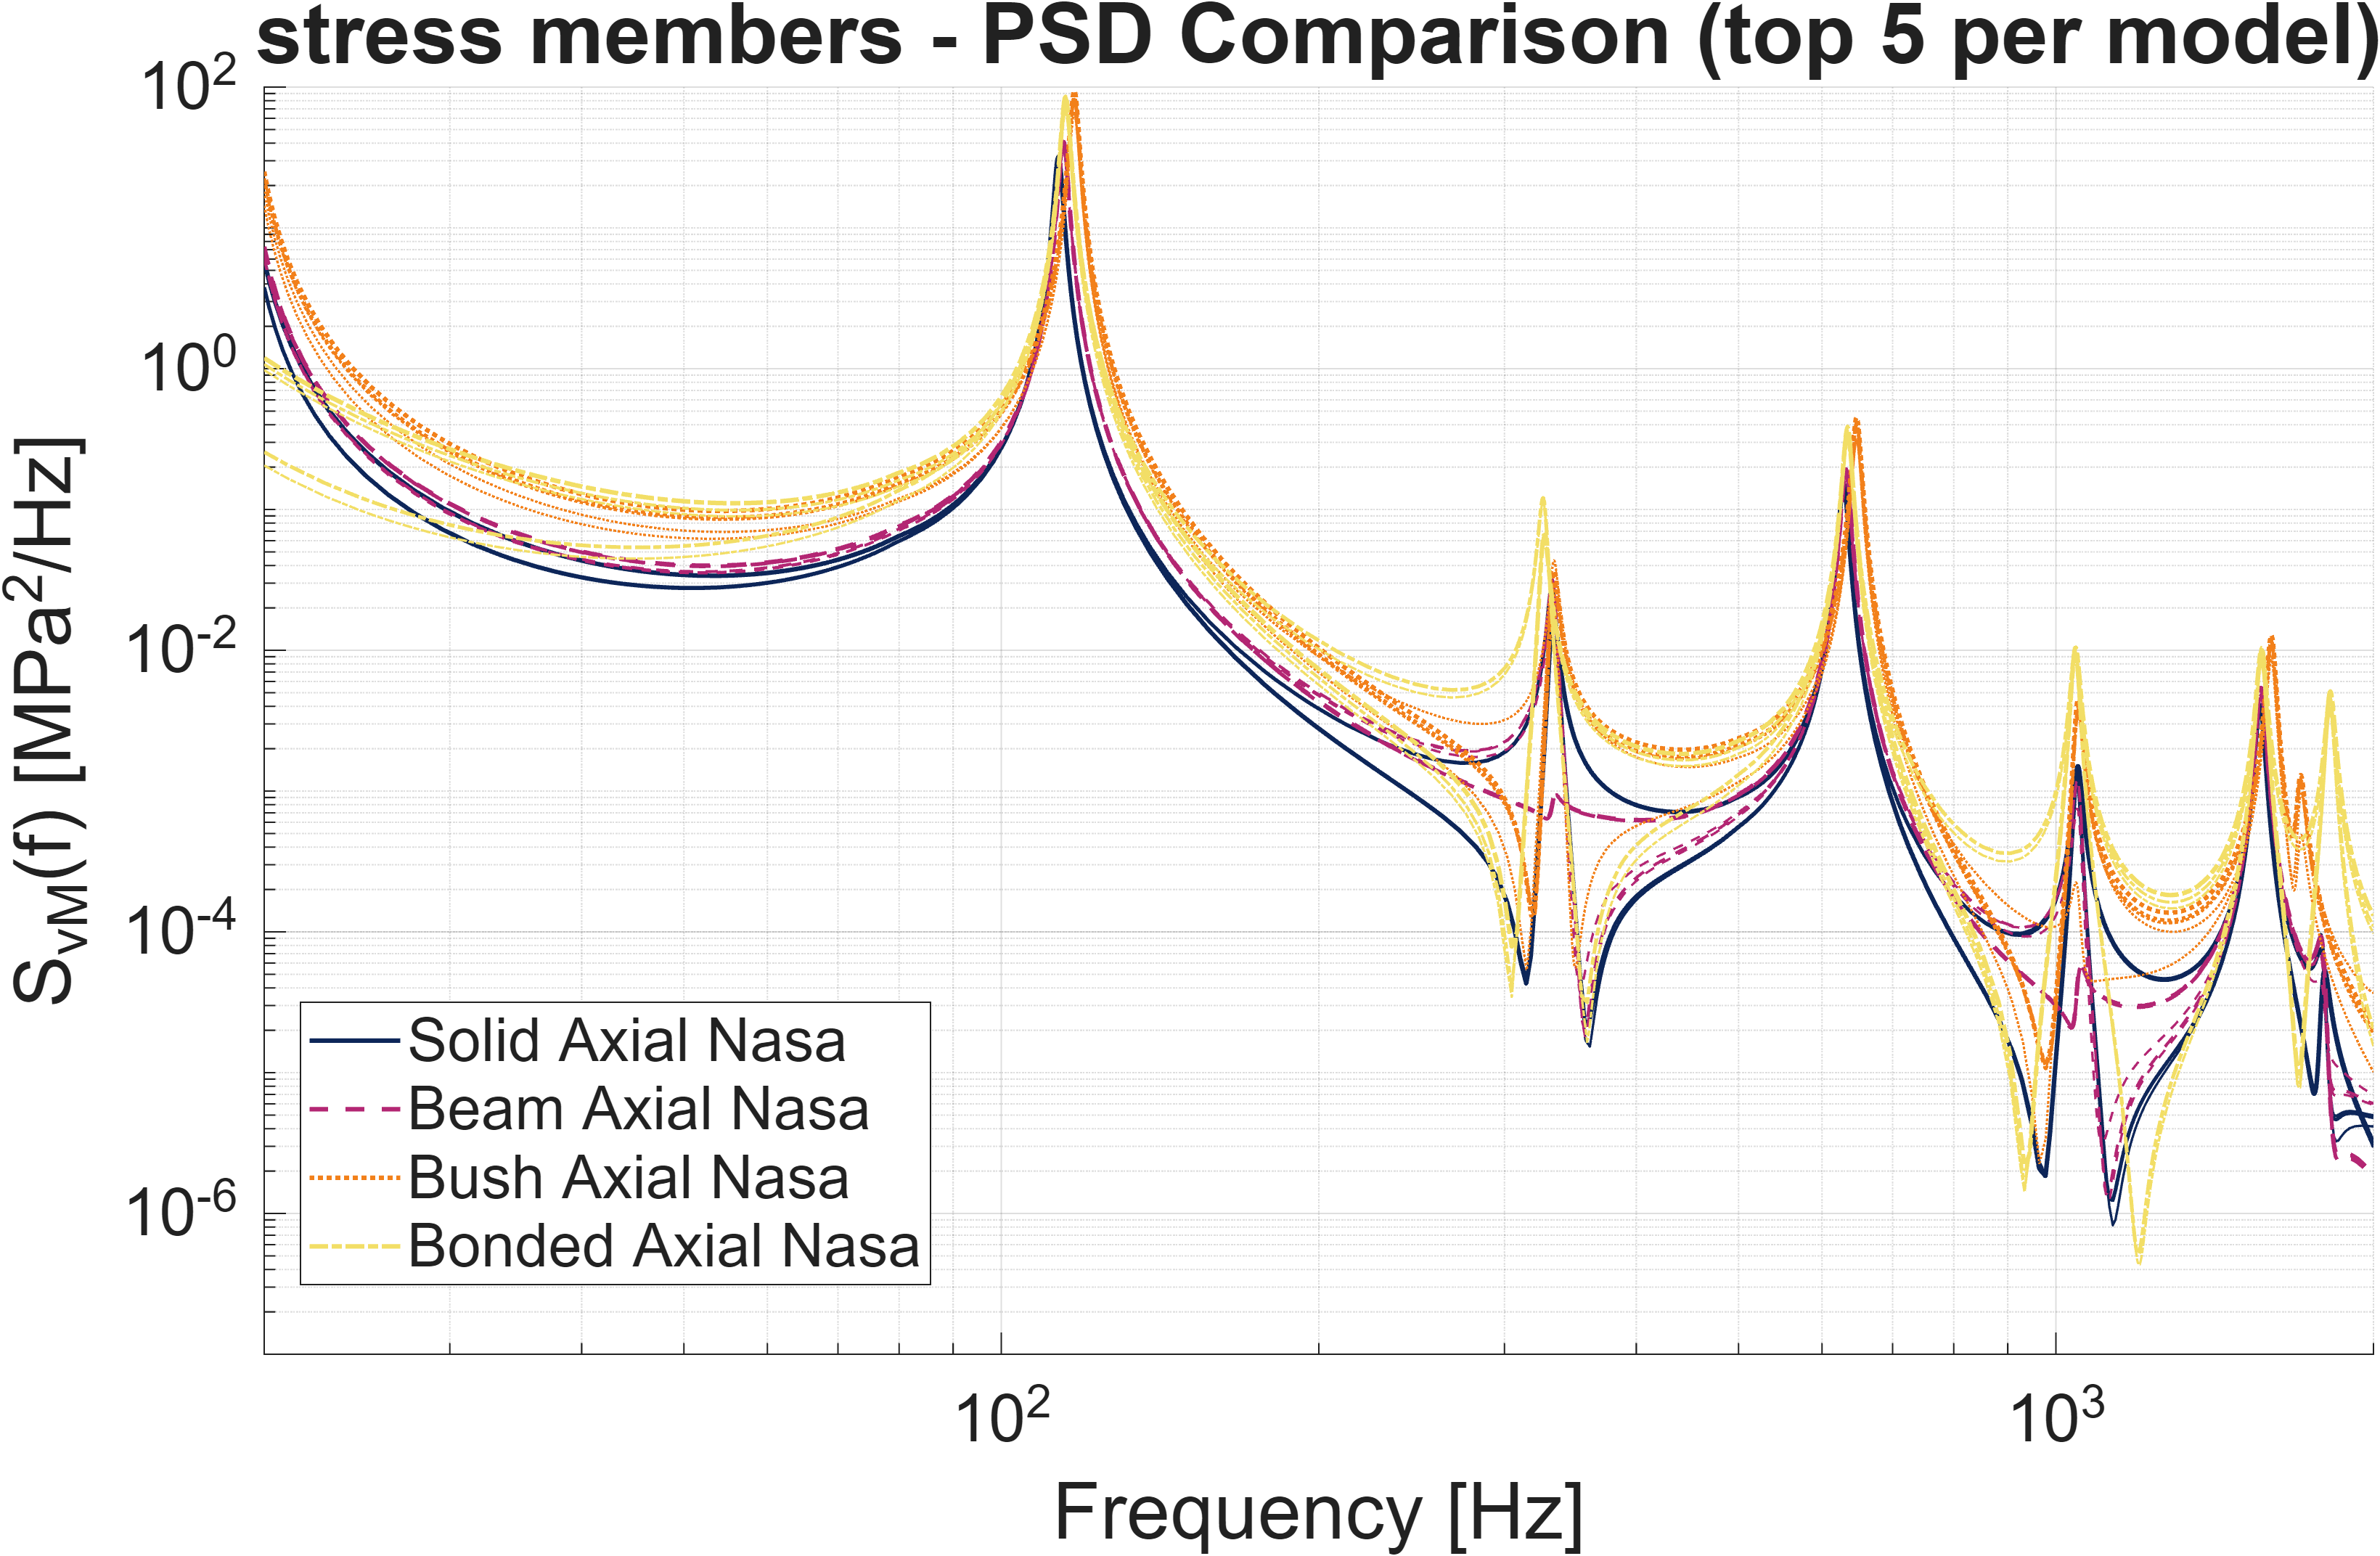
\includegraphics[width=\textwidth]{Axial Nasa/Axial Nasa_psd_overlay_NODEWISE stress_members.png}
        \caption{Axial Loading (bending).}
        \label{fig:NASA_bending_psd_overlay_NODEWISE_stress_members}
    \end{subfigure}
    
\caption{Stress PSDs for the \textit{clamped members} (top 5 per model). All models exhibit resonant peaks at the same fundamental frequencies, but the bonded model shows significantly elevated amplitudes for transverse loading. The same trends are visible in the corresponding T43A results, see Appendix \ref{app:T43A_figures}.}
    \label{fig:Stress_PSD_Members_Comparison}
\end{figure}




\subsection{Bolt Regions: Under-head and First Engaged Thread Region}
Under transverse loading, the beam model produces \ac{PSD} curves of comparable magnitude to the solid model, with peaks at the same frequencies. The beam curves are somewhat higher than the solid curves in both the under-head and at-nut (first-engaged thread) regions, indicating that the beam distributes bearing loads differently than the 3D solid geometry.

Under axial loading, a larger separation appears: at the dominant resonant peaks, the solid model predicts roughly one to two orders of magnitude higher \ac{PSD} values than the beam in the under-head region. This direction dependence is physically expected: When the bolt is tensile-stressed, hotspots form at the underhead fillet, whereas the shaft is more uniformly stressed if only the shaft is pushed.

The key observation is that the beam model does \textit{not} return zero stress in the bolt regions under either loading direction. It returns finite, non-negligible stress \ac{PSD} levels and finite fatigue lives (see Tables \ref{tab:MinLife} - \ref{tab:MinLifeVtical}), unlike the CBUSH and bonded representations.

\begin{figure}[H]
    \centering
    \begin{subfigure}[b]{0.45\textwidth}
        \centering
        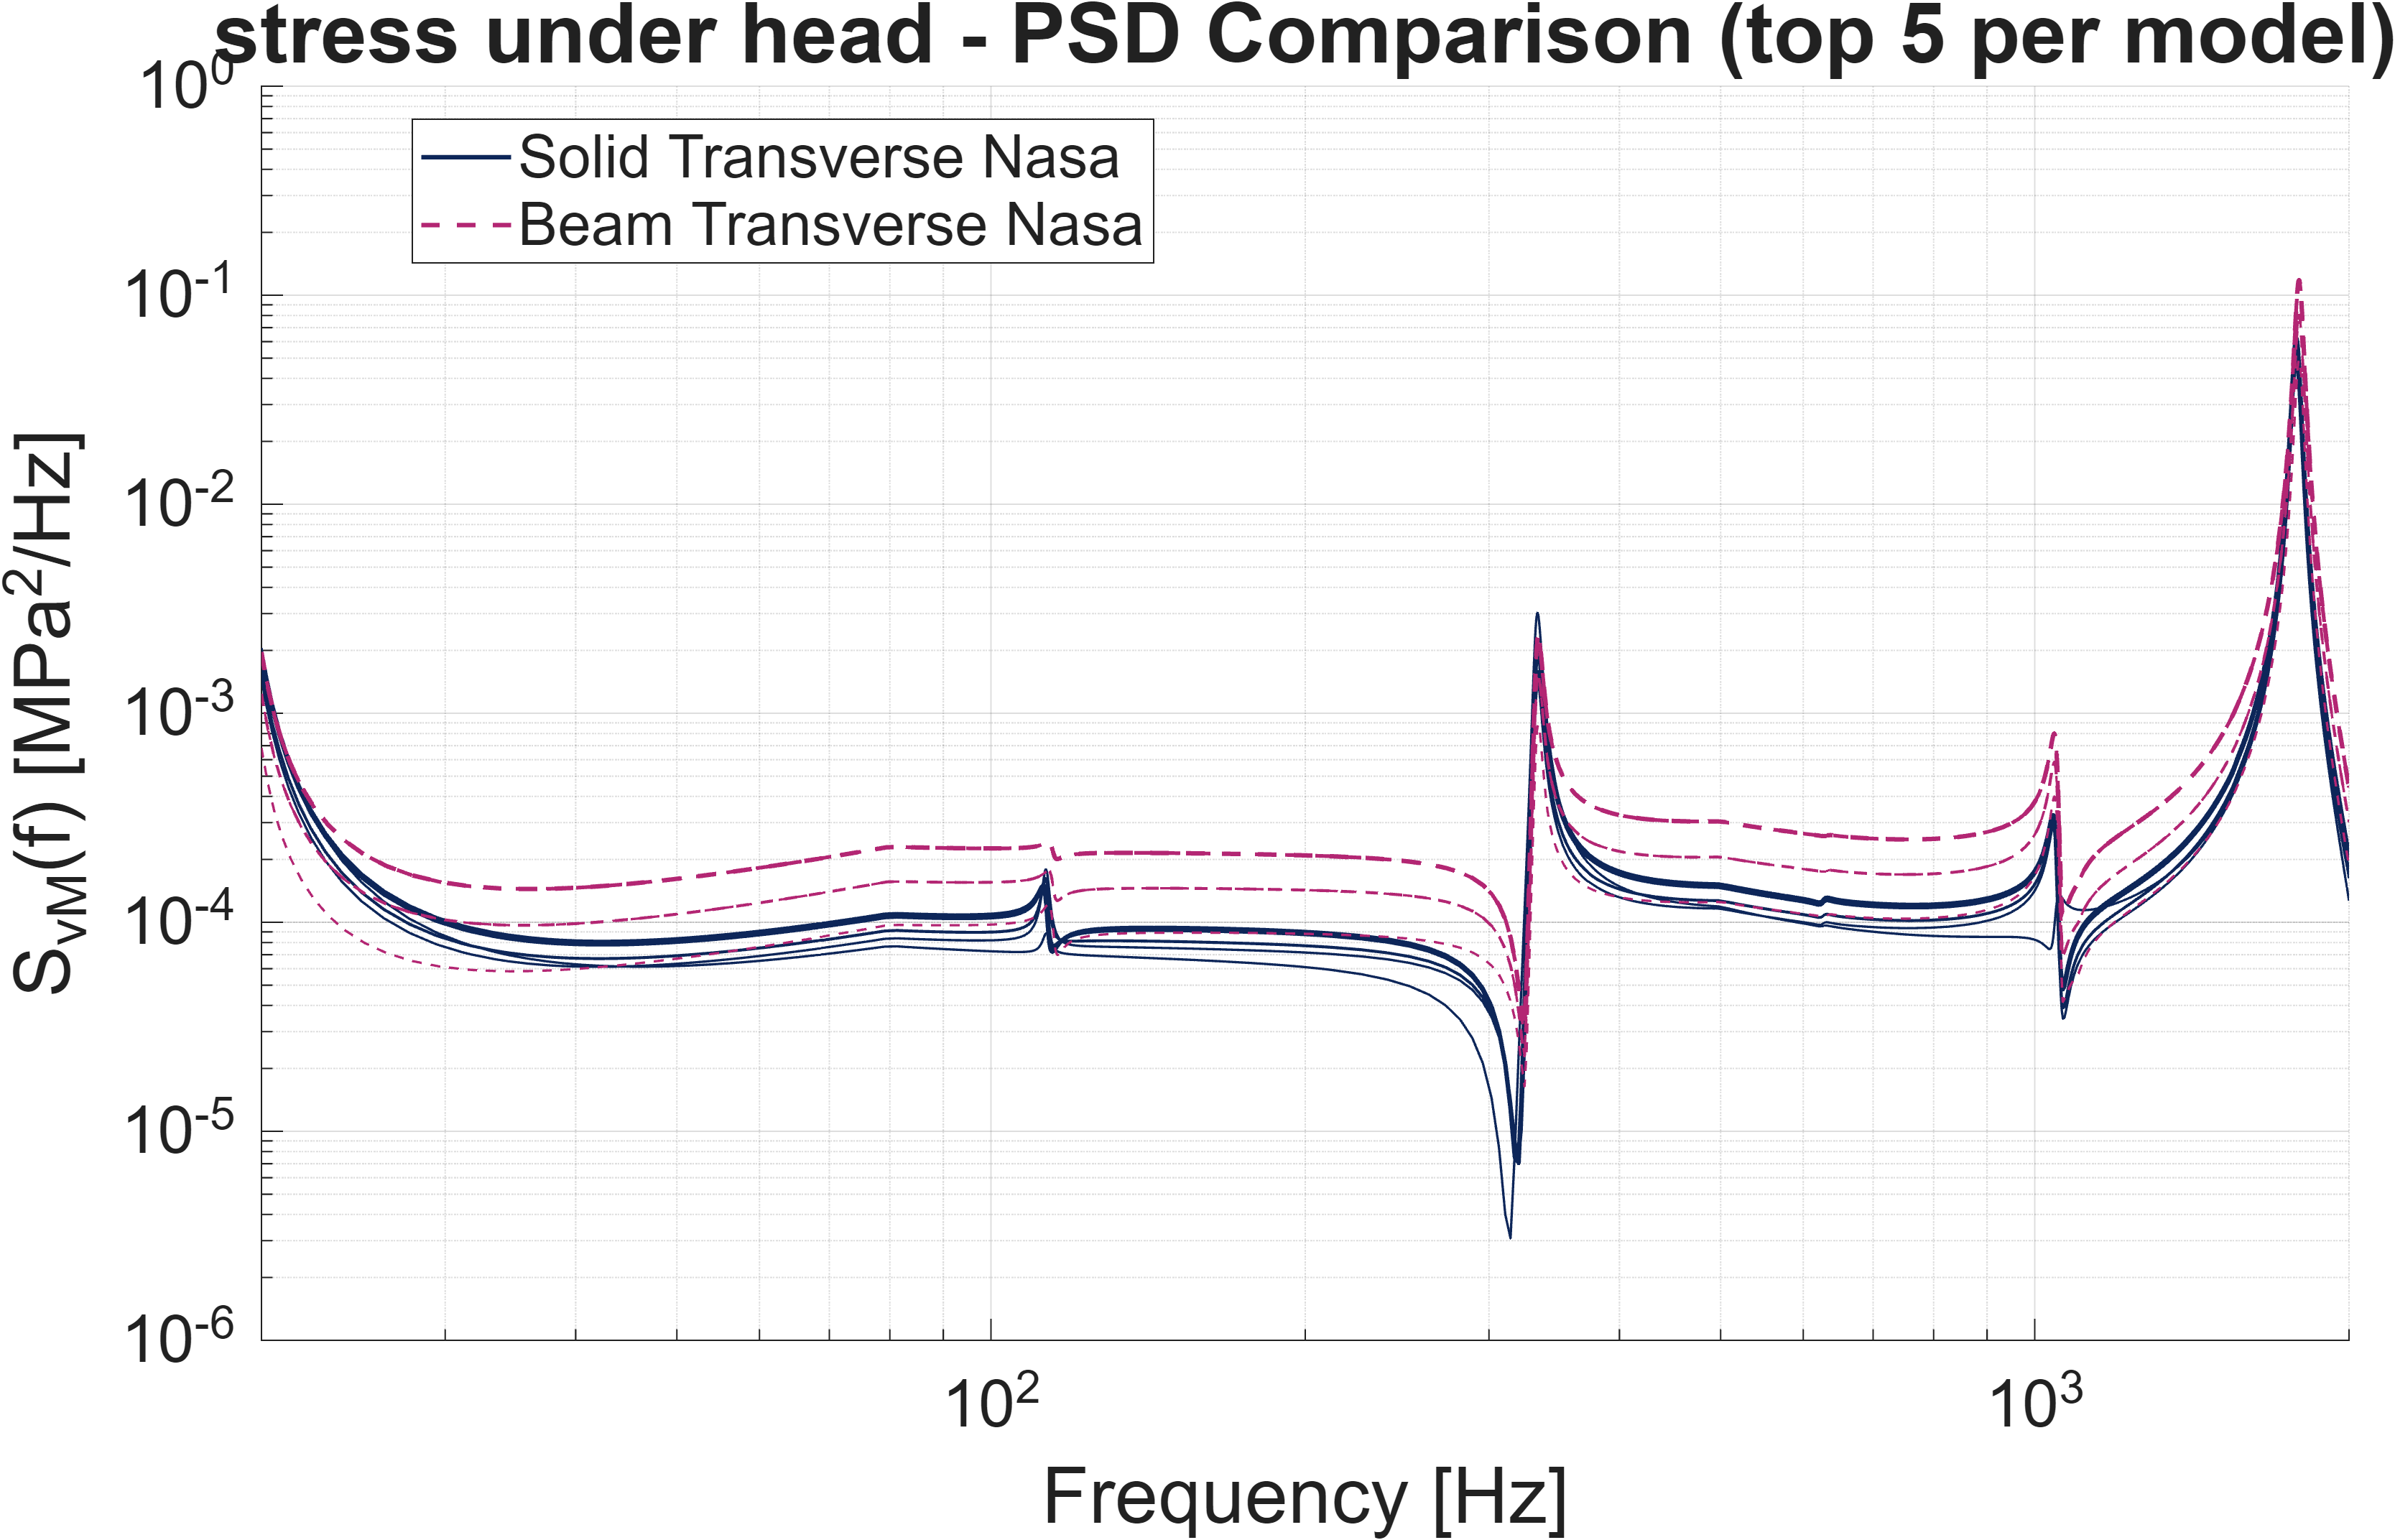
\includegraphics[width=\textwidth]{Transverse Nasa/Transverse Nasa_psd_overlay_NODEWISE stress_under_head.png}
        \caption{Transverse Loading (shear).}
        \label{fig:NASA_shear_psd_overlay_NODEWISE_stress_under_head}
    \end{subfigure}
    \begin{subfigure}[b]{0.45\textwidth}
        \centering
        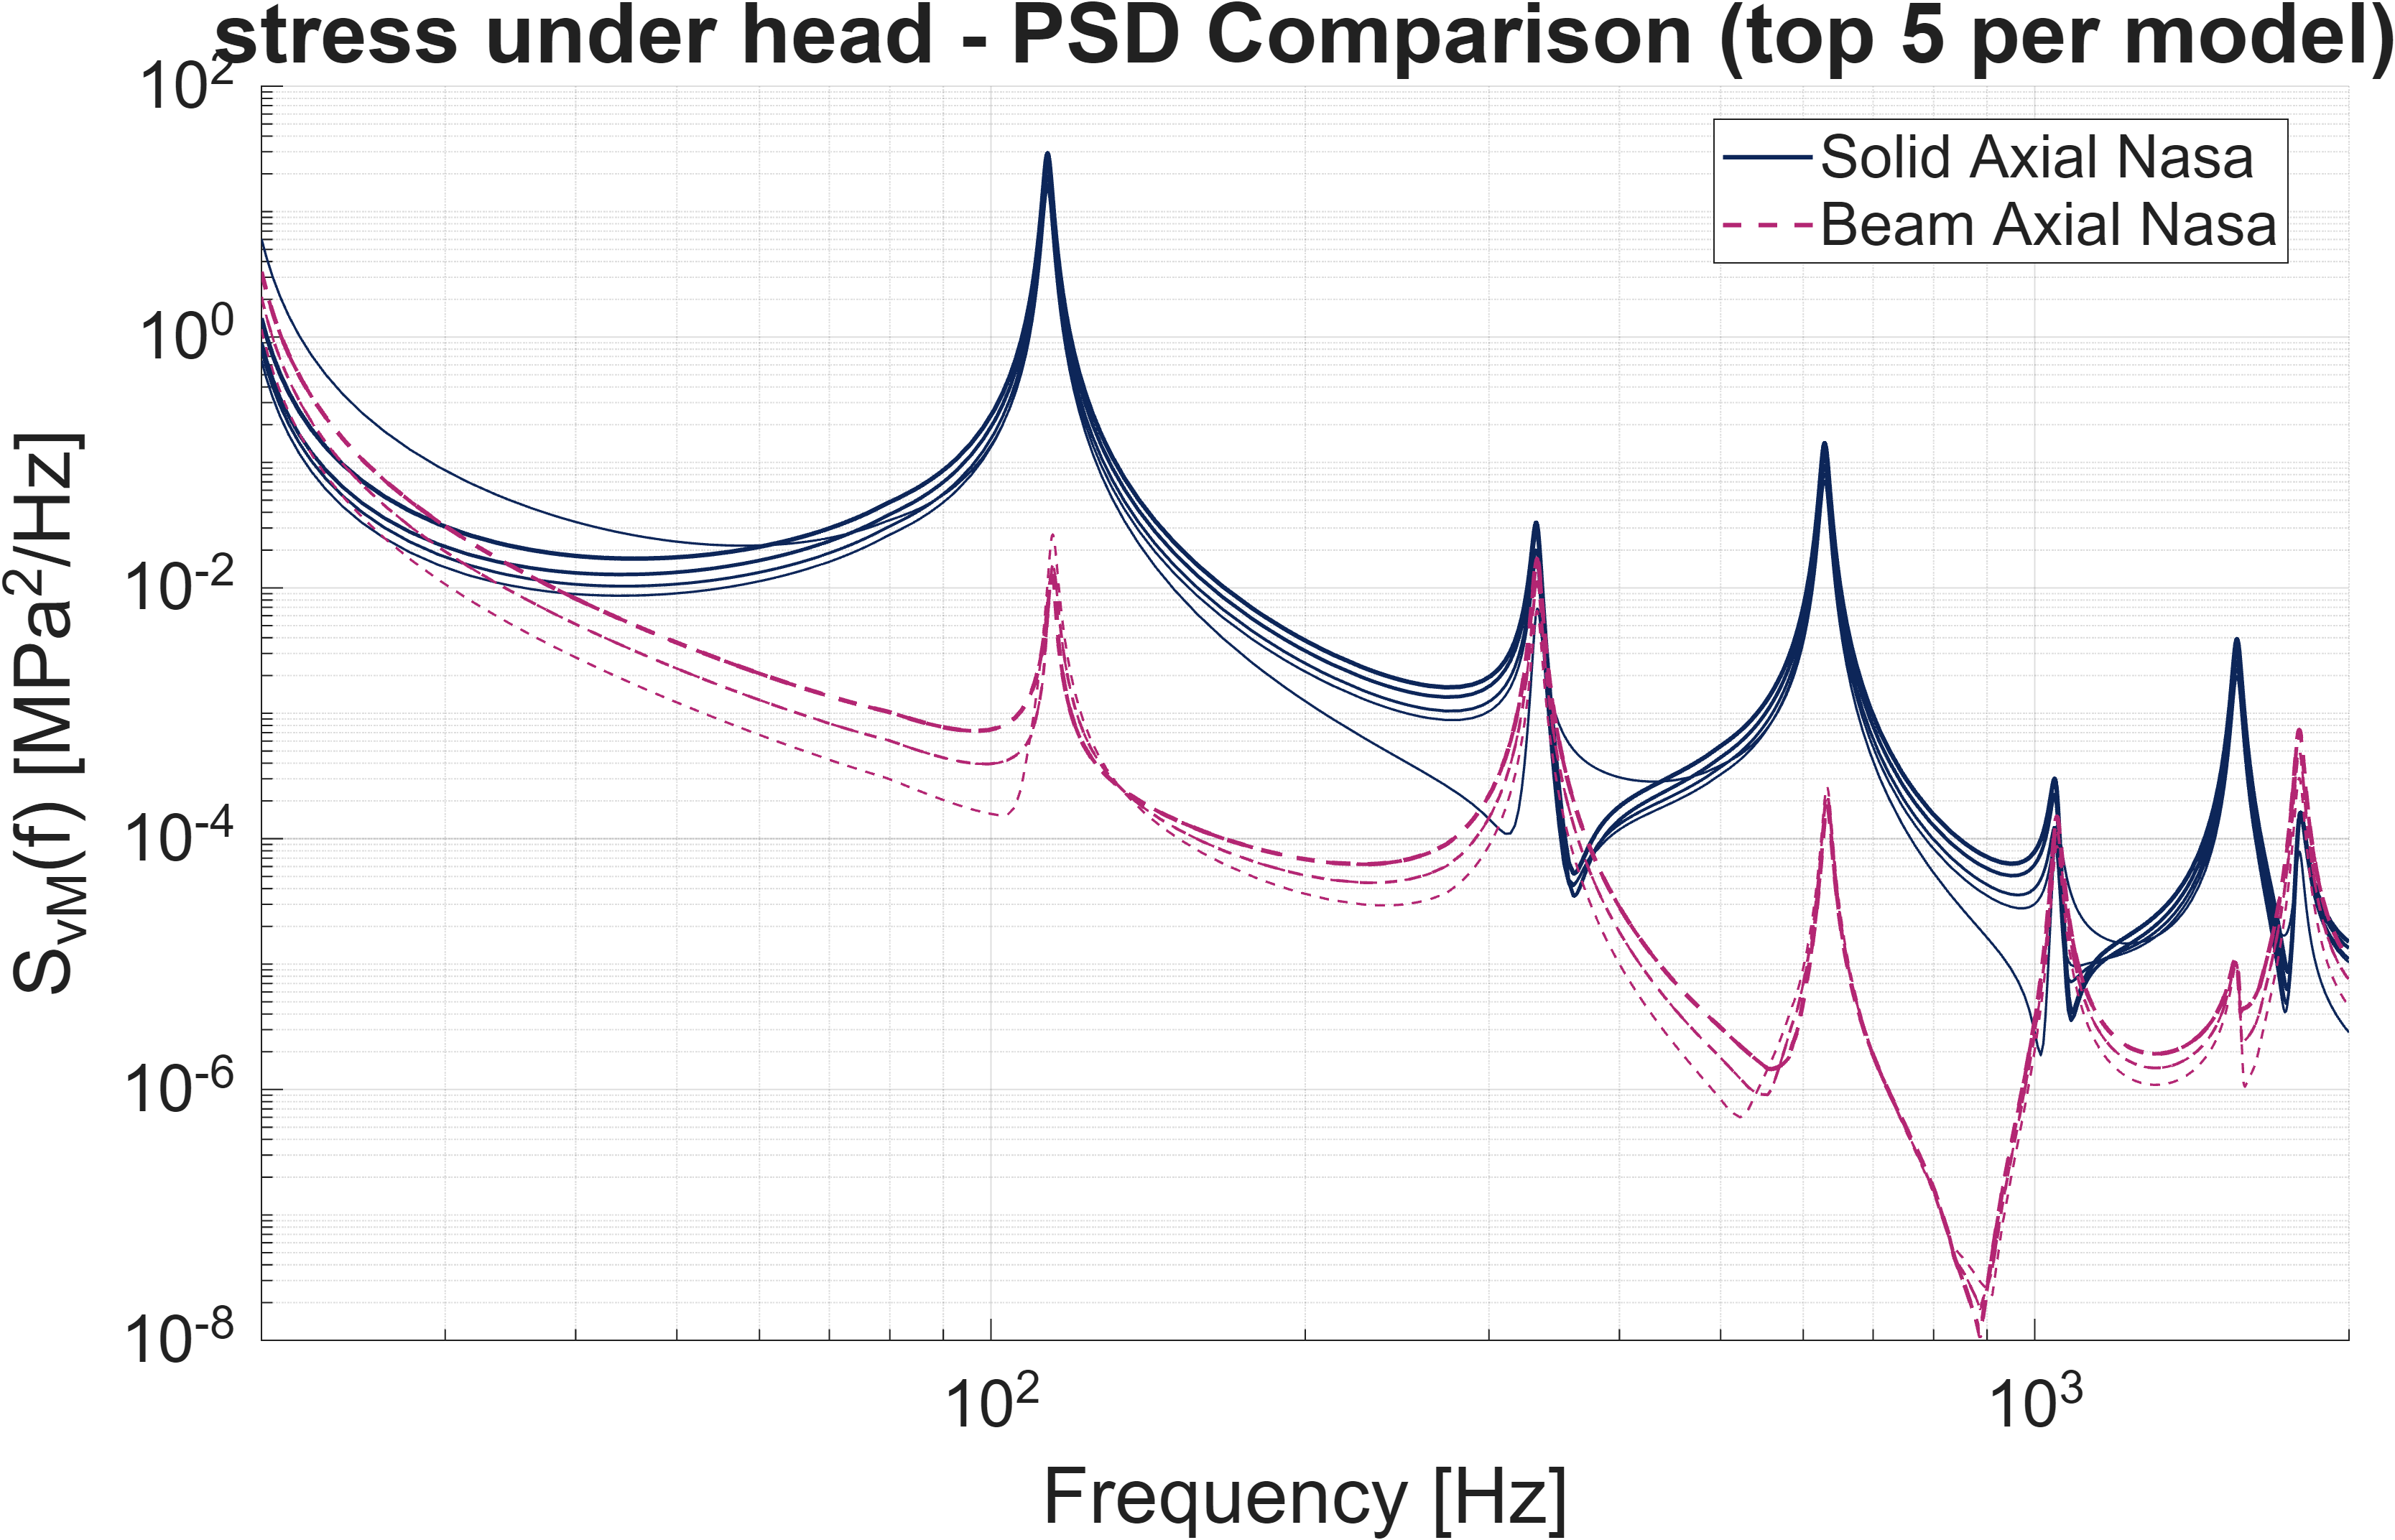
\includegraphics[width=\textwidth]{Axial Nasa/Axial Nasa_psd_overlay_NODEWISE stress_under_head.png}
        \caption{Axial Loading (bending).}
        \label{fig:NASA_bending_psd_overlay_NODEWISE_stress_under_head}
    \end{subfigure}
    
    \caption{Stress PSDs for the \textit{stress under-head fillet} (top 5 nodes per model). Left: transverse loading, right: axial loading. The beam model returns non-zero stress in both directions, but deviates from the solid under axial loading. The same trends are visible in the corresponding T43A results, see Appendix \ref{app:T43A_figures}.}
    \label{fig:Stress_PSD_UnderHead_Comparison}
\end{figure}

\begin{figure}[H]
    \centering
    \begin{subfigure}[b]{0.45\textwidth}
        \centering
        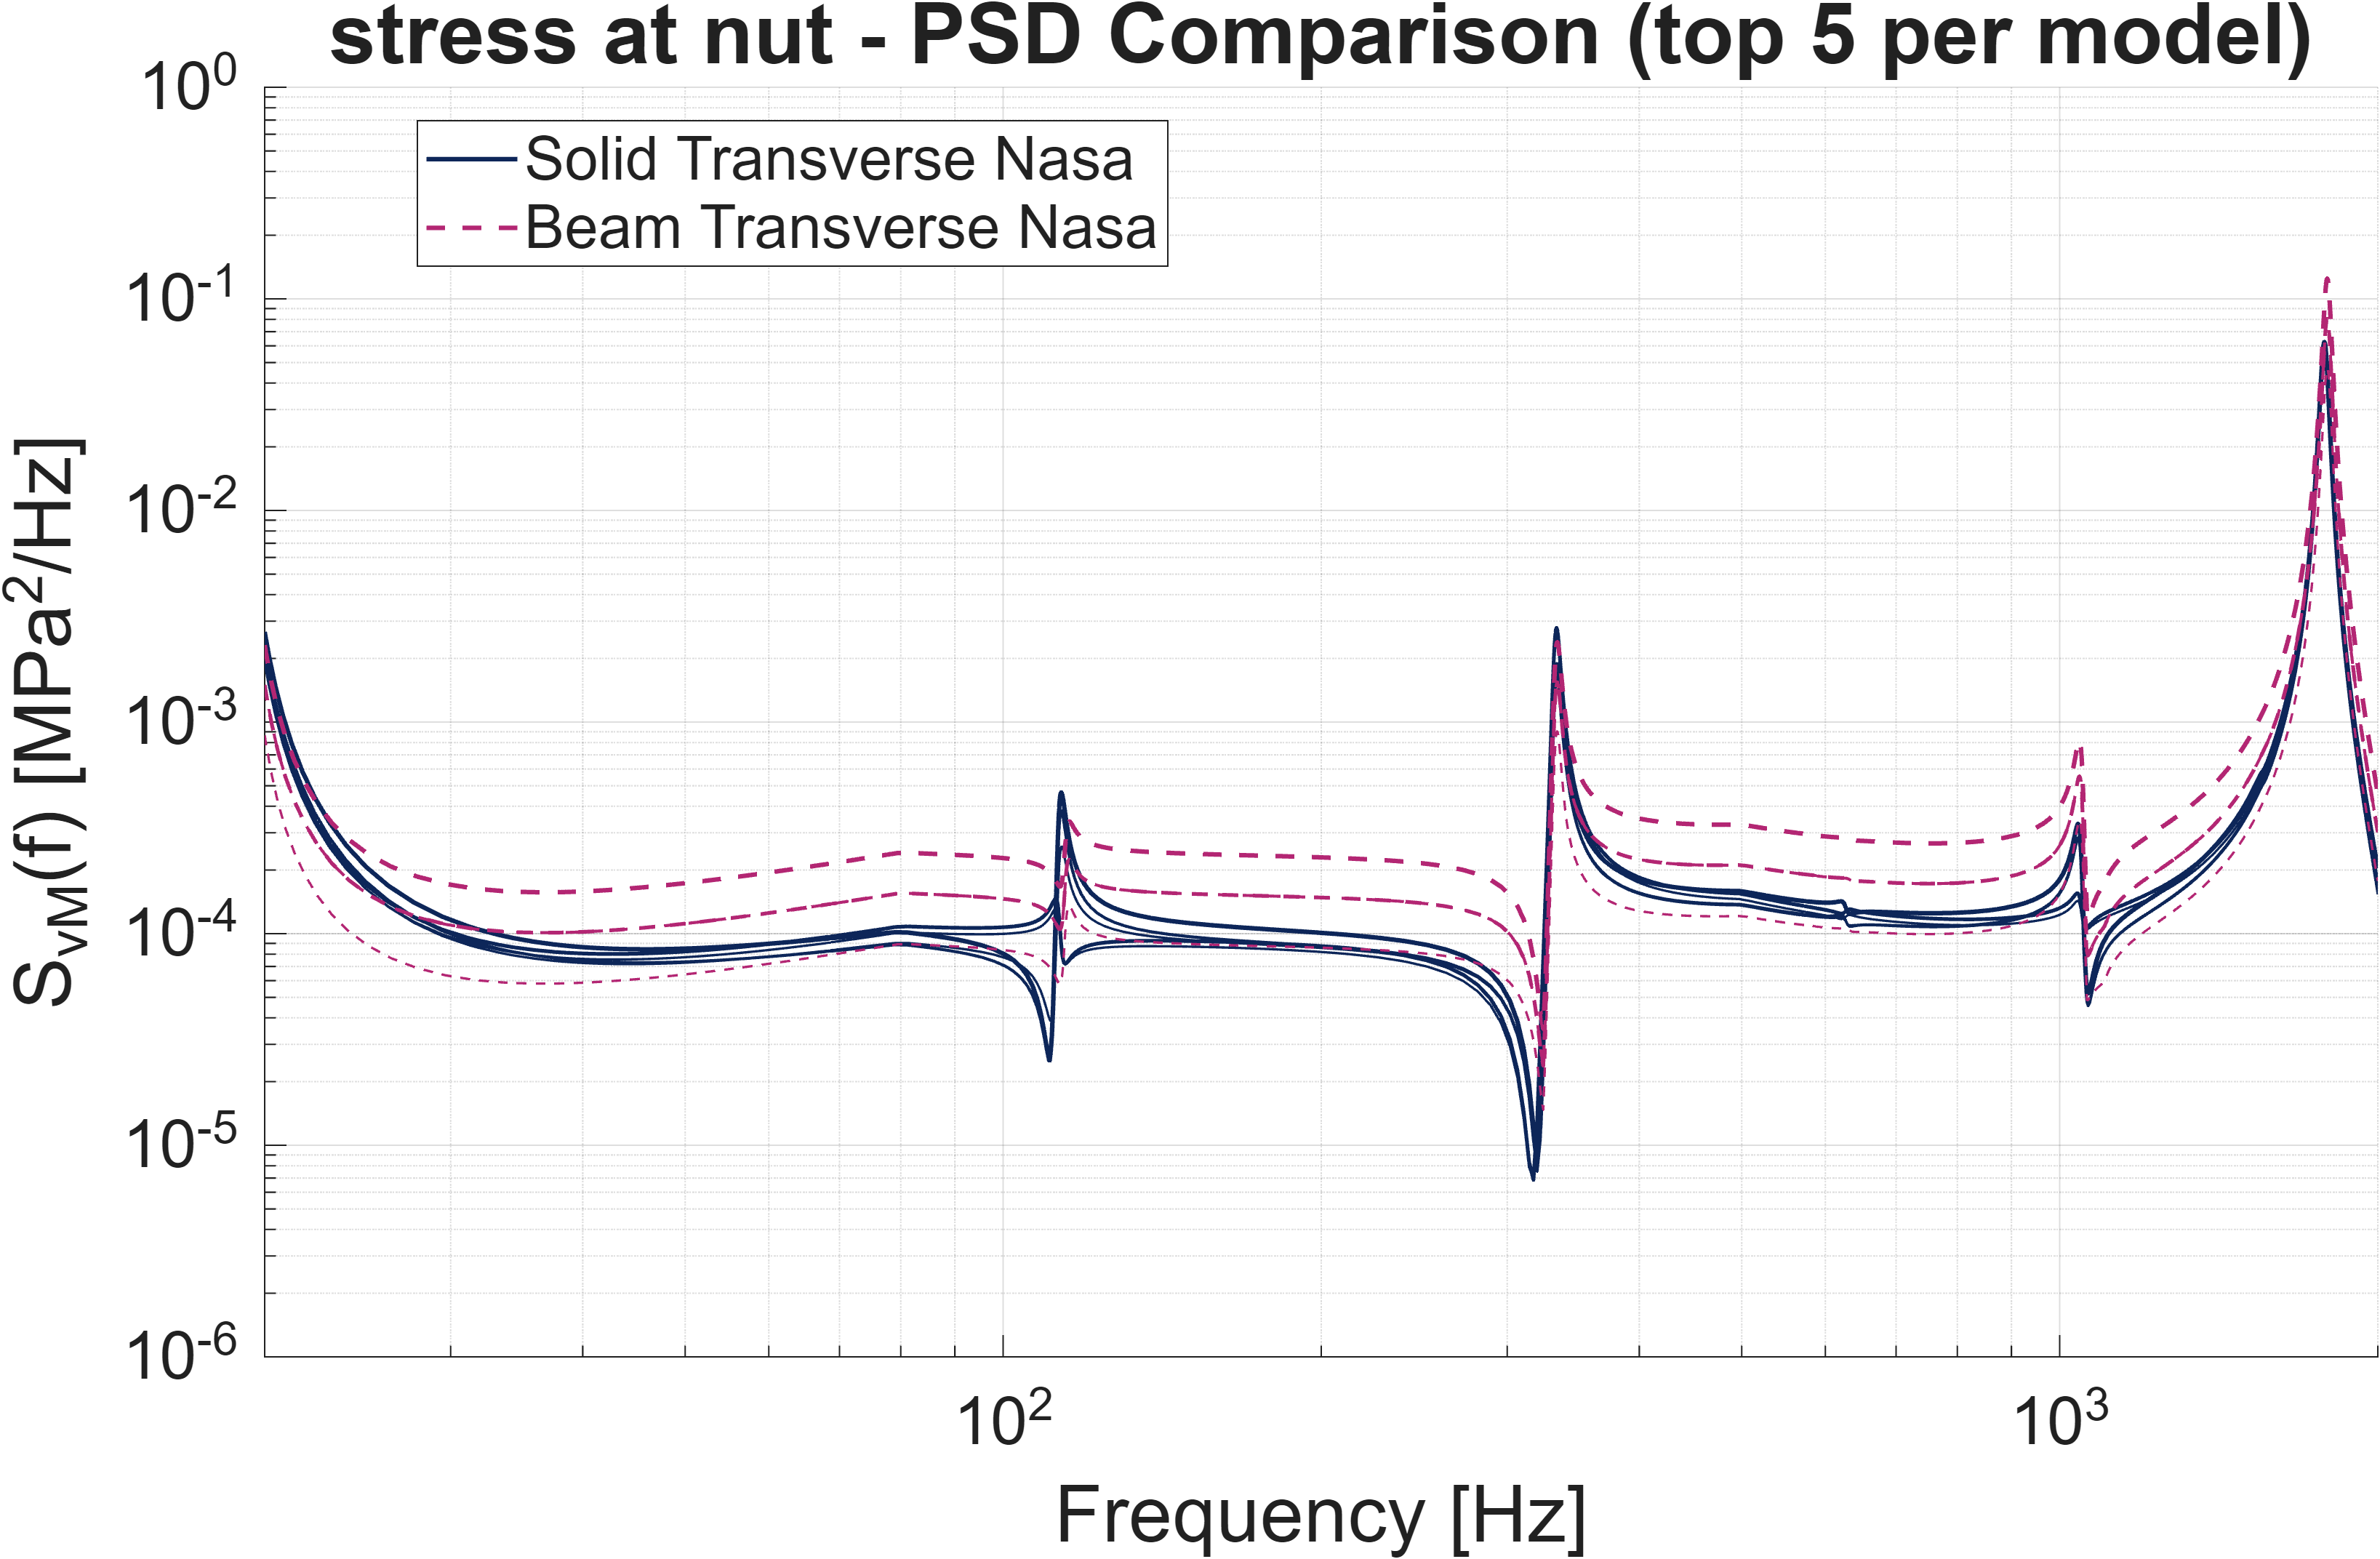
\includegraphics[width=\textwidth]{Transverse Nasa/Transverse Nasa_psd_overlay_NODEWISE stress_at_nut.png}
        \caption{Transverse Loading (shear).}
        \label{fig:NASA_shear_psd_overlay_NODEWISE_stress_at_nut}
    \end{subfigure}
    \begin{subfigure}[b]{0.45\textwidth}
        \centering
        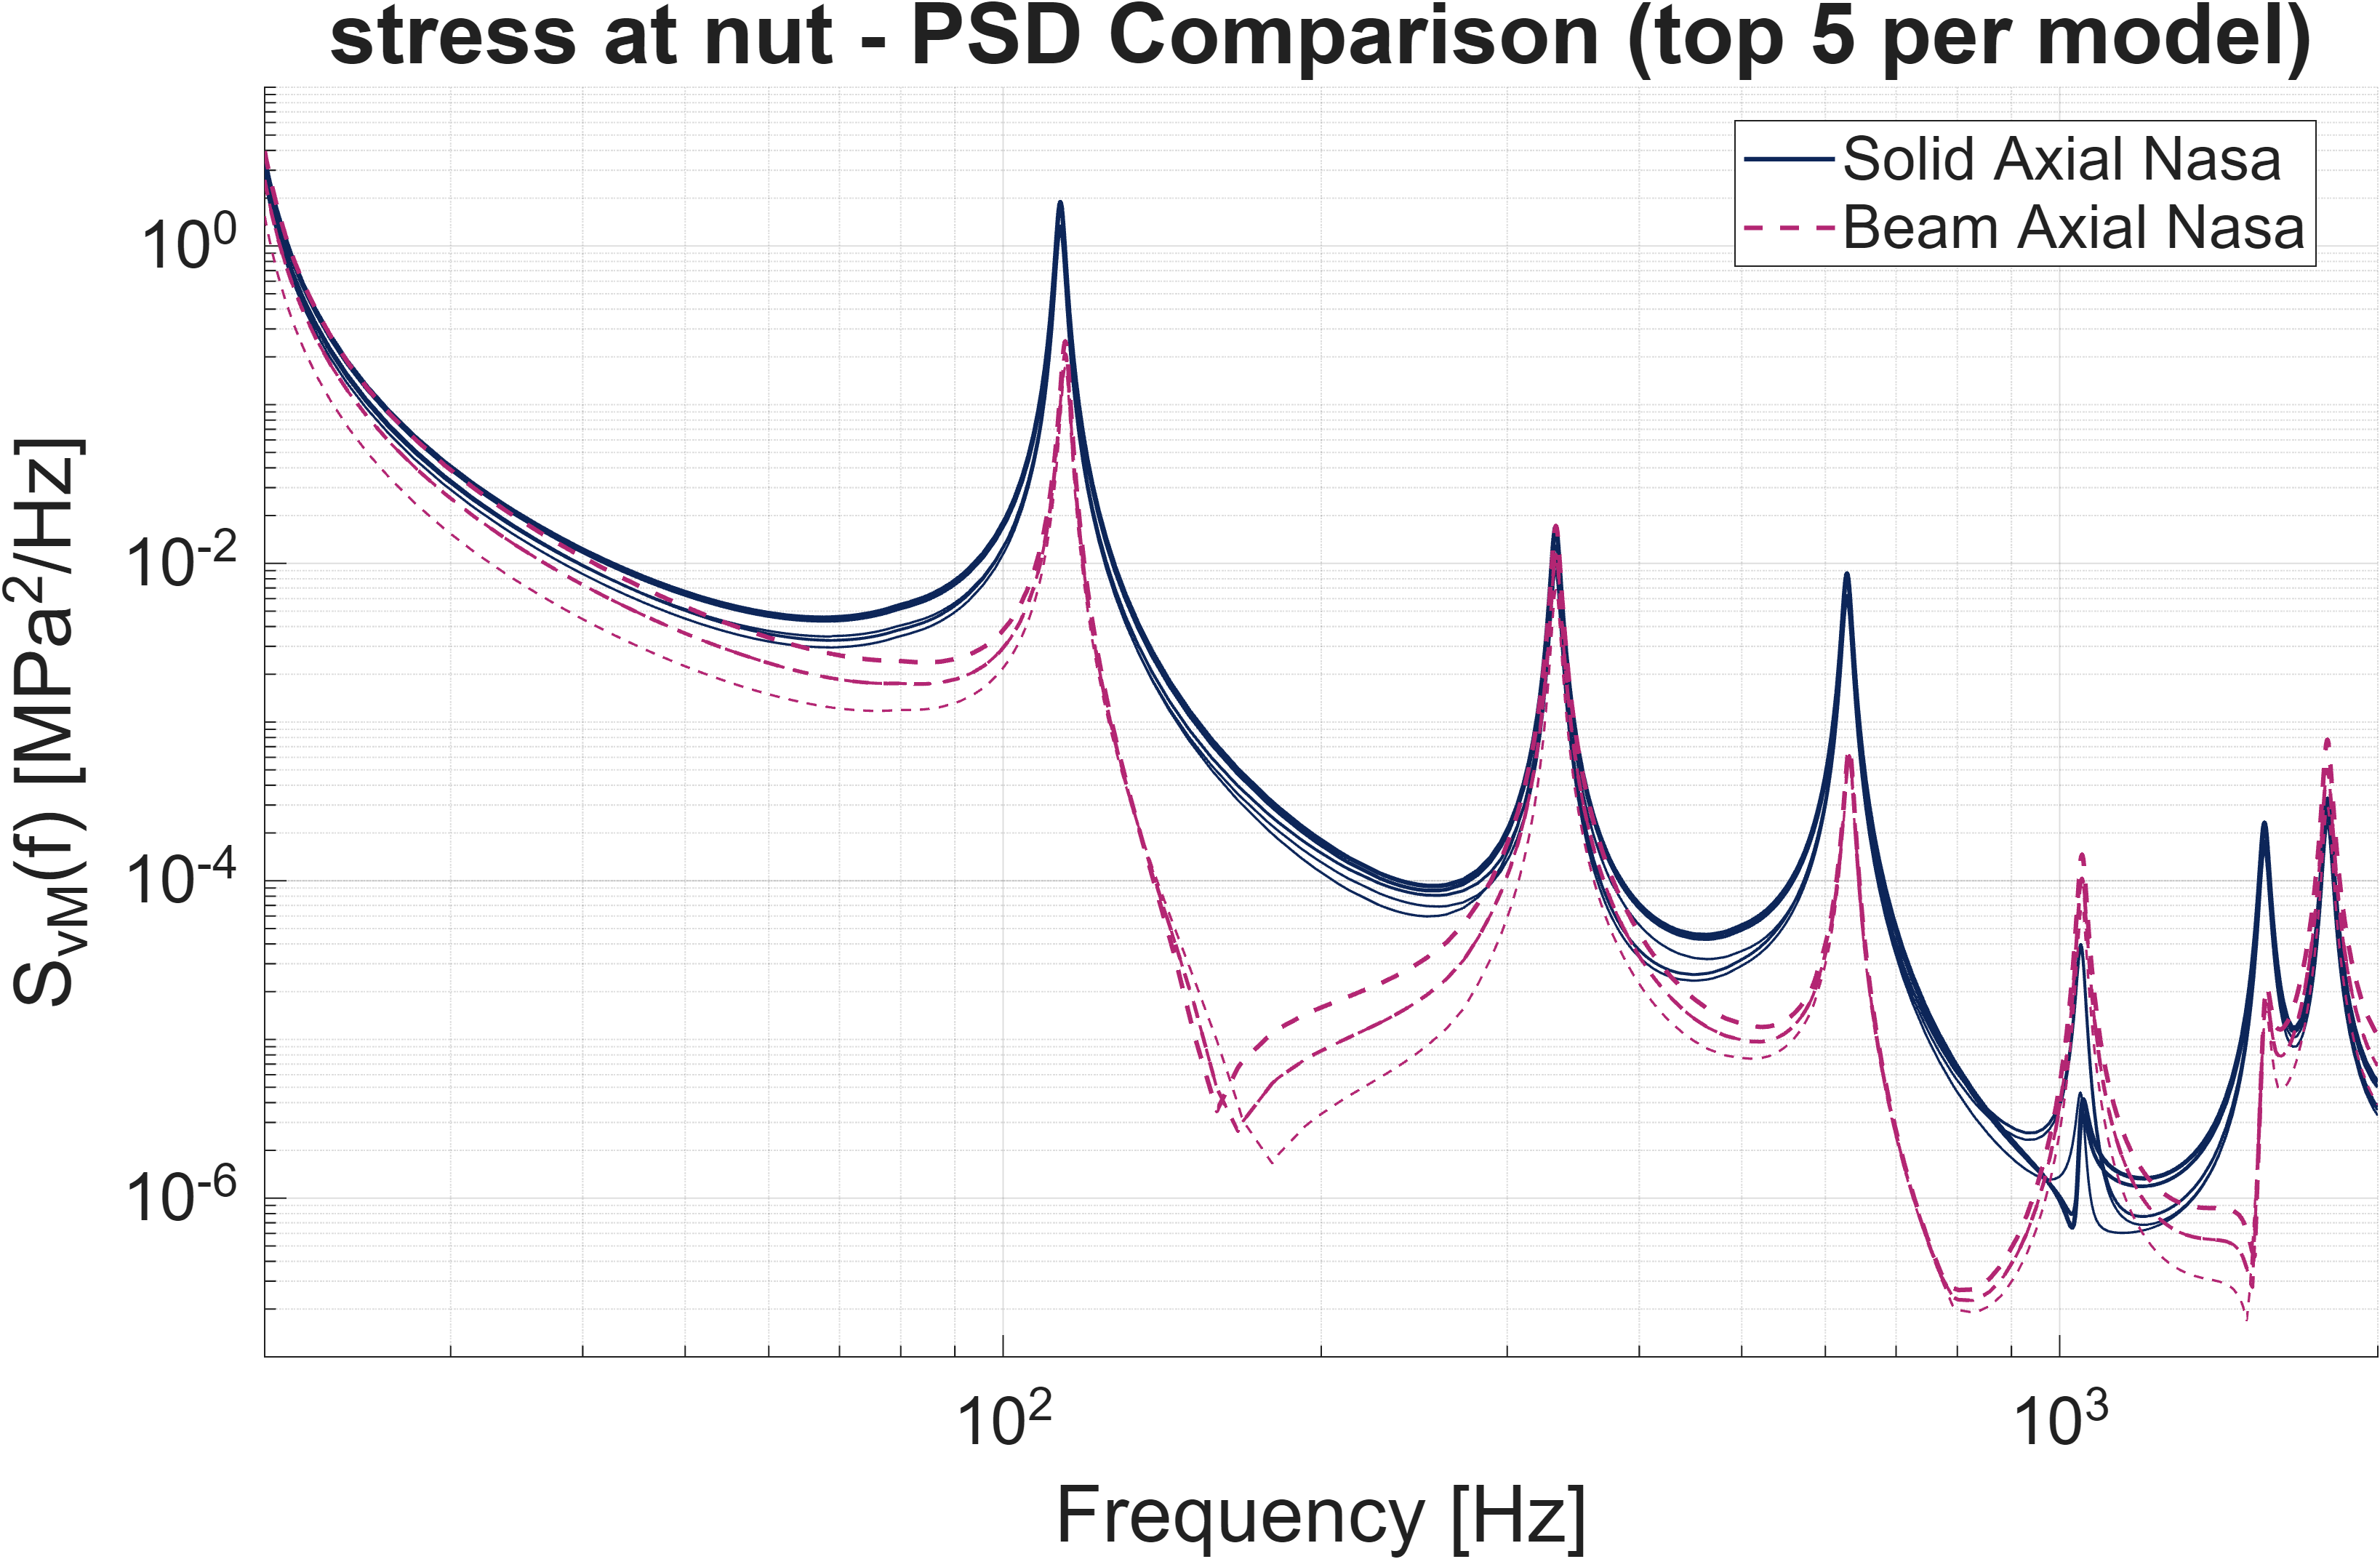
\includegraphics[width=\textwidth]{Axial Nasa/Axial Nasa_psd_overlay_NODEWISE stress_at_nut.png}
        \caption{Axial Loading (bending).}
        \label{fig:NASA_bending_psd_overlay_NODEWISE_stress_at_nut}
    \end{subfigure}
    \caption{Stress \ac{PSD} for the \textit{stress at nut} (top 5 nodes per model). Both models predict finite stress, the beam overpredicts the \ac{RMS} under transverse loading and underpredicts under axial loading relative to the solid. The same trends are visible in the corresponding T43A results, see Appendix \ref{app:T43A_figures}.}
    \label{fig:Stress_PSD_AtNut_Comparison}
\end{figure}

The stress \ac{PSD} comparisons provide the basis for the fatigue-life results that follow. Any model that overpredicts the stress \ac{PSD} level in the clamped members should also predict shorter fatigue life. Still, local bolt fatigue cannot be meaningfully assessed unless the model explicitly resolves those regions.

\newpage
\section{Fatigue life comparison} \label{sec:FatigueLifeCompare}

Once the stress \ac{PSD} has been established, the corresponding \ac{RMS} stress level and fatigue life can be evaluated for each extraction region, model, and loading direction.

Table \ref{tab:MinLife} summarizes the minimum Dirlik fatigue life, and Table \ref{tab:MaxRMS_HorizNASA}-\ref{tab:MaxRMS_VertNASA} summarizes the maximum \ac{RMS} von Mises stress for each extraction region and model. The corresponding bar charts are shown in Figure \ref{fig:RMS_per_region} and Figure \ref{fig:Life_per_region}. The most meaningful comparison is obtained in the clamped members region, because that is the only region where all four models produce directly comparable stress results. To give a physical sense of the scale: the lives reported in the clamped members range from roughly $2 \times 10^6$ s for the bonded model (about 2 weeks of continuous excitation) to $2.7 \times 10^7$ s for the solid reference (about 10 months of continuous excitation). 

\begin{table}[H]
    \centering
    \caption{Minimum nodewise Goodman-corrected Dirlik life: Transverse Loading (NASA Workmanship)}
    \label{tab:MinLife}
    \begin{tabular}{lcccc}
        \toprule
        Region          & Bonded               & Beam                  & Solid                 & CBUSH                  \\
        \midrule
        Clamped Members & $1.97\times10^{6}$ s & $2.30\times10^{7}$ s  & $2.71\times10^{7}$ s  & $7.16\times10^{6}$ s  \\
        under-head fillet   & -                   & $7.09\times10^{7}$ s  & $4.63\times10^{6}$ s  & -                    \\
        First Engaged   & -                   & $6.37\times10^{7}$ s  & $4.57\times10^{6}$ s  & -                    \\
        \bottomrule
    \end{tabular}
\end{table}

\begin{table}[H]
    \centering
    \caption{Minimum nodewise Goodman-corrected Dirlik life: Axial Loading (NASA Workmanship)}
    \label{tab:MinLifeVtical}
    \begin{tabular}{lcccc}
        \toprule
        Region          & Bonded               & Beam                  & Solid                 & CBUSH                  \\
        \midrule
        Clamped Members & $3.73\times10^{5}$ s & $1.60\times10^{6}$ s  & $2.68\times10^{6}$ s  & $2.71\times10^{5}$ s  \\
        under-head fillet   & -                   & $4.84\times10^{9}$ s  & $3.41\times10^{6}$ s  & -                    \\
        First Engaged   & -                   & $2.15\times10^{9}$ s  & $3.80\times10^{8}$ s  & -                    \\
        \bottomrule
    \end{tabular}
\end{table}

\begin{table}[H]
    \centering
    \caption{Maximum \ac{RMS} Stress: Axial Loading (NASA Workmanship)}
    \label{tab:MaxRMS_HorizNASA}
    \begin{tabular}{lcccc}
        \toprule
        Region & Bonded contact & Beam & Solid no threads & CBUSH spring \\
        \midrule
        Clamped Members & 6.38 MPa$_{RMS}$ & 3.48 MPa$_{RMS}$ & 3.34 MPa$_{RMS}$ & 4.68 MPa$_{RMS}$ \\
        under-head fillet & -              & 2.62 MPa$_{RMS}$ & 1.90 MPa$_{RMS}$ & -                \\
        First Engaged   & -                & 2.69 MPa$_{RMS}$ & 1.91 MPa$_{RMS}$ & -                \\
        \bottomrule
    \end{tabular}
\end{table}

\begin{table}[H]
    \centering
    \caption{Maximum \ac{RMS} Stress: Transverse Loading (NASA Workmanship)}
    \label{tab:MaxRMS_VertNASA}
    \begin{tabular}{lcccc}
        \toprule
        Region & Bonded contact & Beam & Solid no threads & CBUSH spring \\
        \midrule
        Clamped Members & 18.3 MPa$_{RMS}$ & 12.8 MPa$_{RMS}$ & 11.3 MPa$_{RMS}$ & 19.9 MPa$_{RMS}$ \\
        under-head fillet & -              & 2.38 MPa$_{RMS}$ & 10.5 MPa$_{RMS}$ & -                \\
        First Engaged   & -                & 2.76 MPa$_{RMS}$ & 3.66 MPa$_{RMS}$ & -                \\
        \bottomrule
    \end{tabular}
\end{table}
The local bolt regions of the solid bolt predict around $4.6 \times 10^6$, or roughly 7 weeks. These are not service-life estimates - they are equivalent durations under uninterrupted NASA-Workmanship excitation and serve only to compare the four models.

The same trends are visualized in Figure \ref{fig:RMS_per_region} and \ref{fig:Life_per_region}. Figure \ref{fig:RMS_per_region} shows that, in the clamped members region, the beam model remains close to the reference, while the CBUSH and especially the bonded model predict much larger \ac{RMS} stress. Figure \ref{fig:Life_per_region} shows the corresponding Dirlik fatigue life. As expected from the SN-curve, the higher the predicted stress, the shorter the predicted life.


\begin{figure}[H]
    \centering
    \begin{subfigure}[b]{0.45\textwidth}
        \centering
        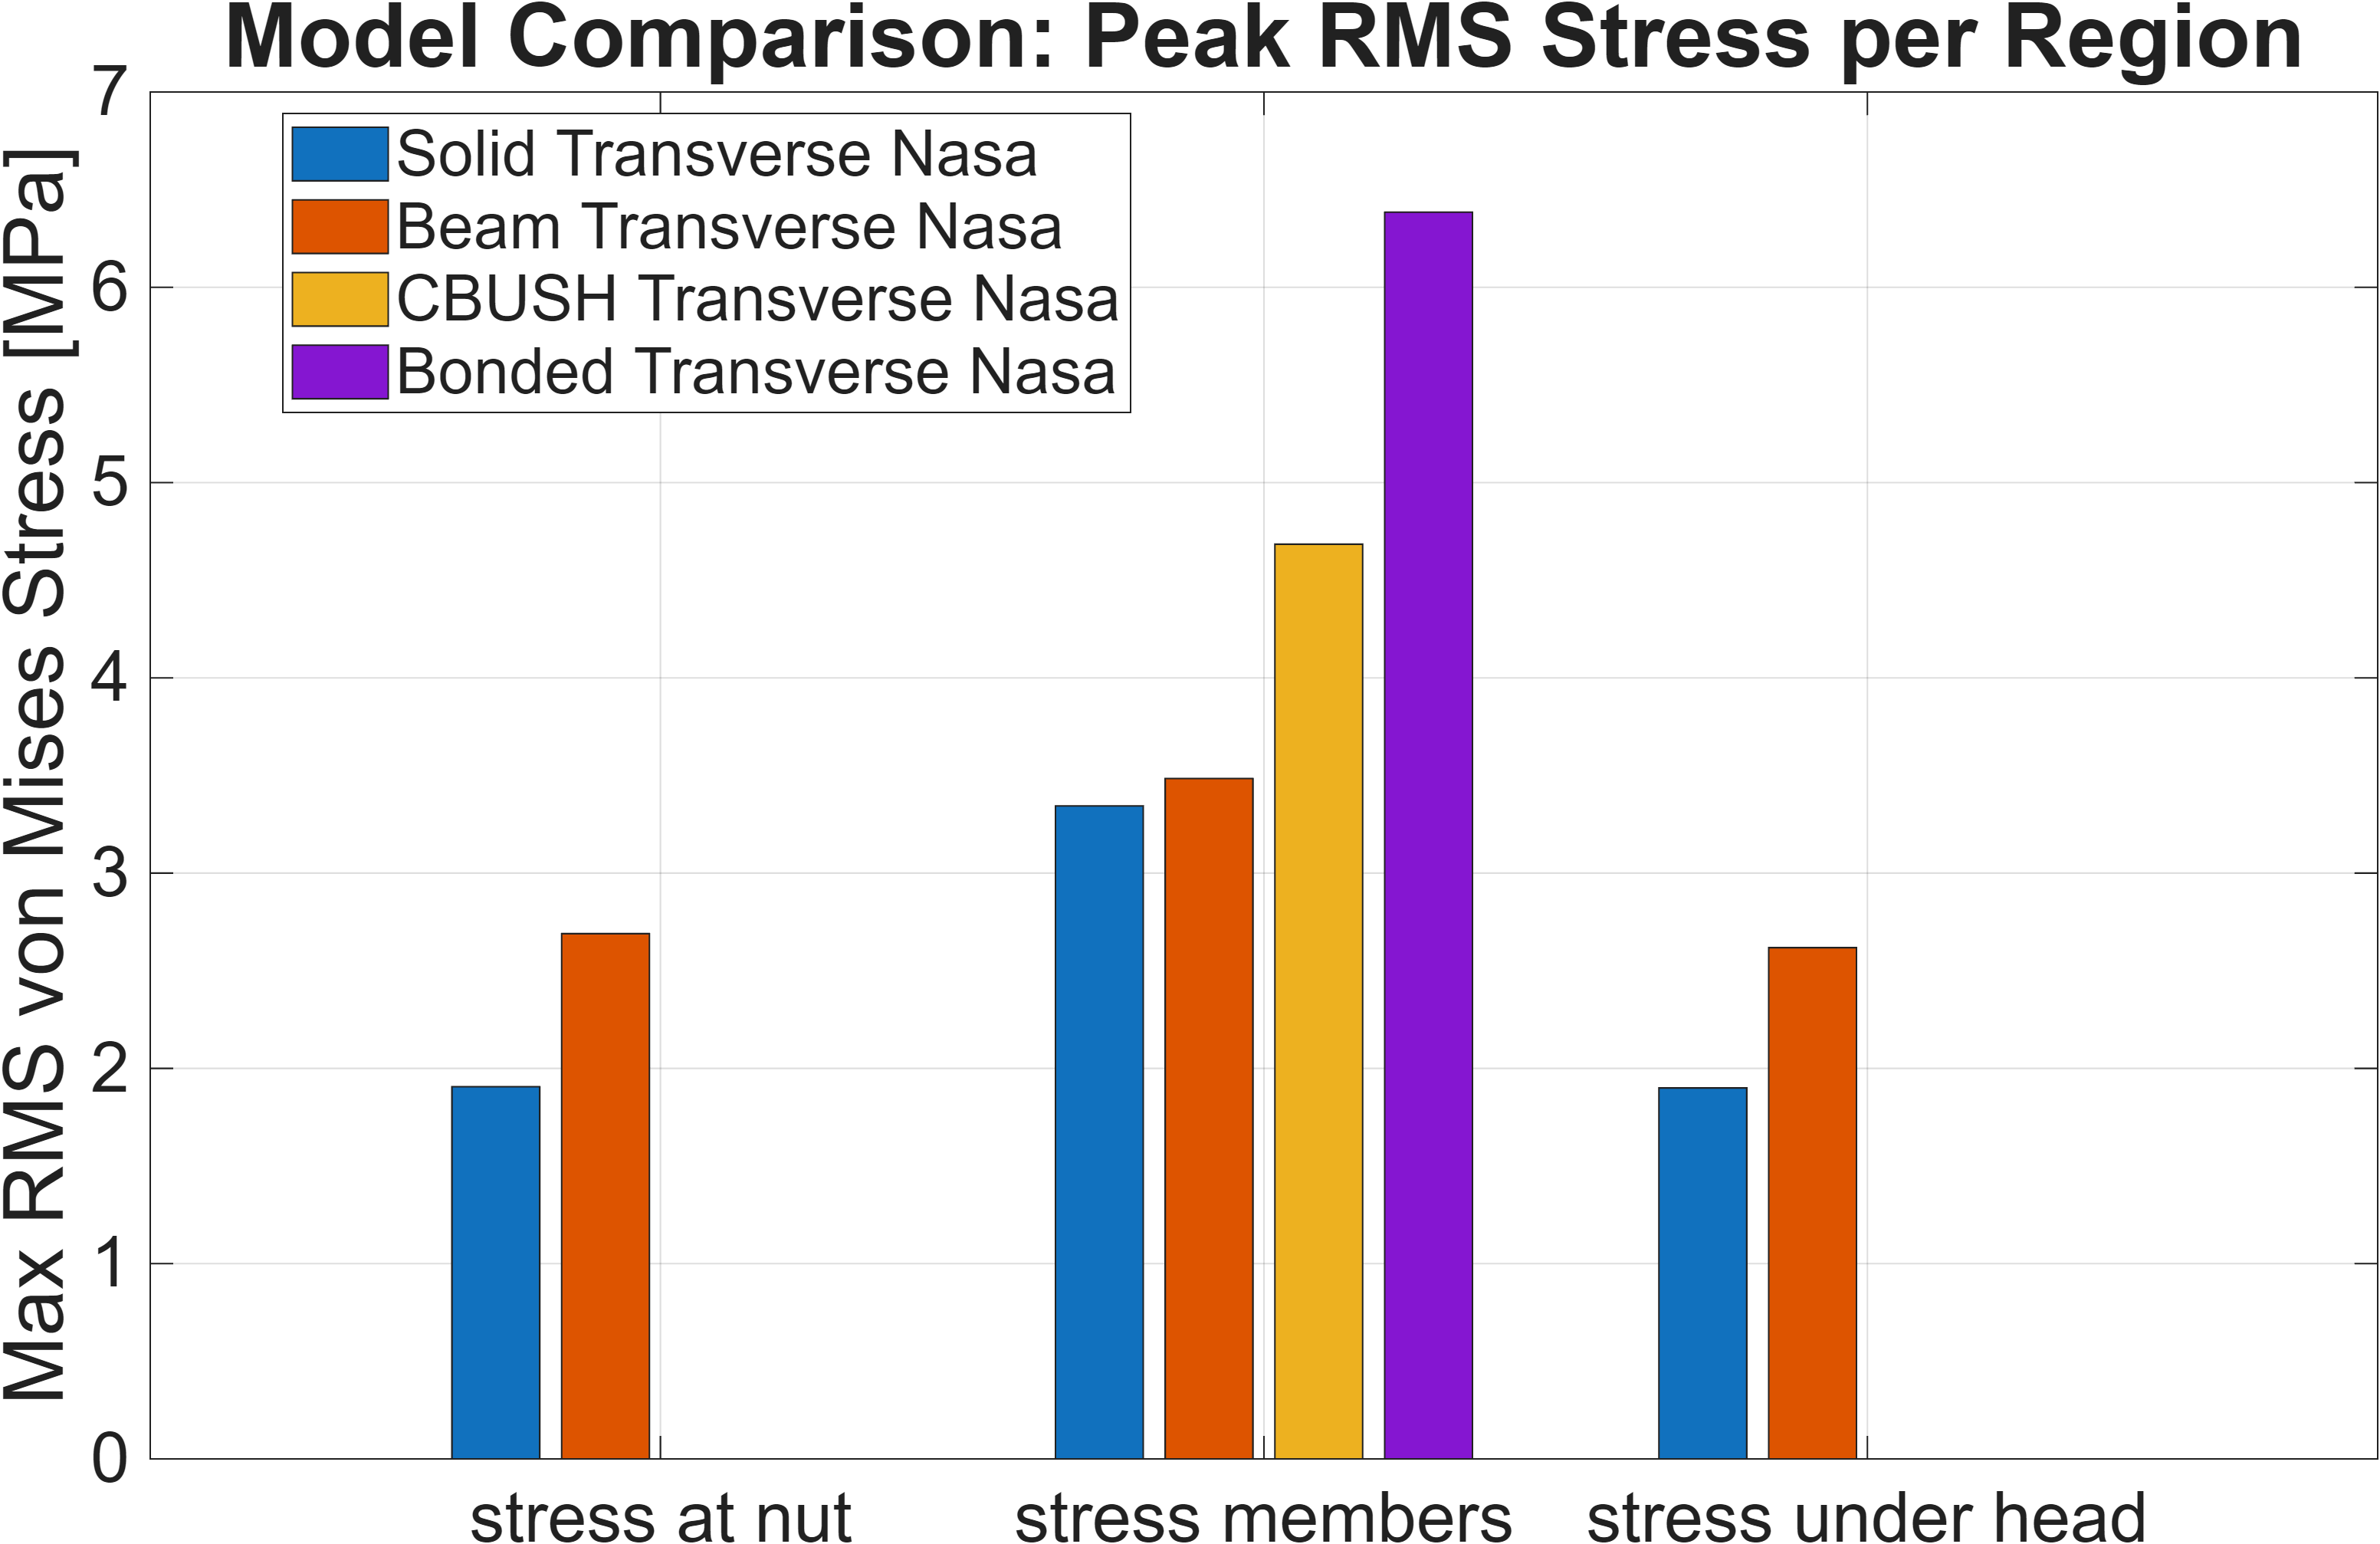
\includegraphics[width=\textwidth]{Transverse Nasa/Transverse Nasa_comparison_max_rms_per_region NODEWISE.png}
        \caption{Transverse Loading (shear).}
        \label{fig:NASA_shear_comparison_max_rms_per_region_NODEWISE}
    \end{subfigure}
    \begin{subfigure}[b]{0.45\textwidth}
        \centering
        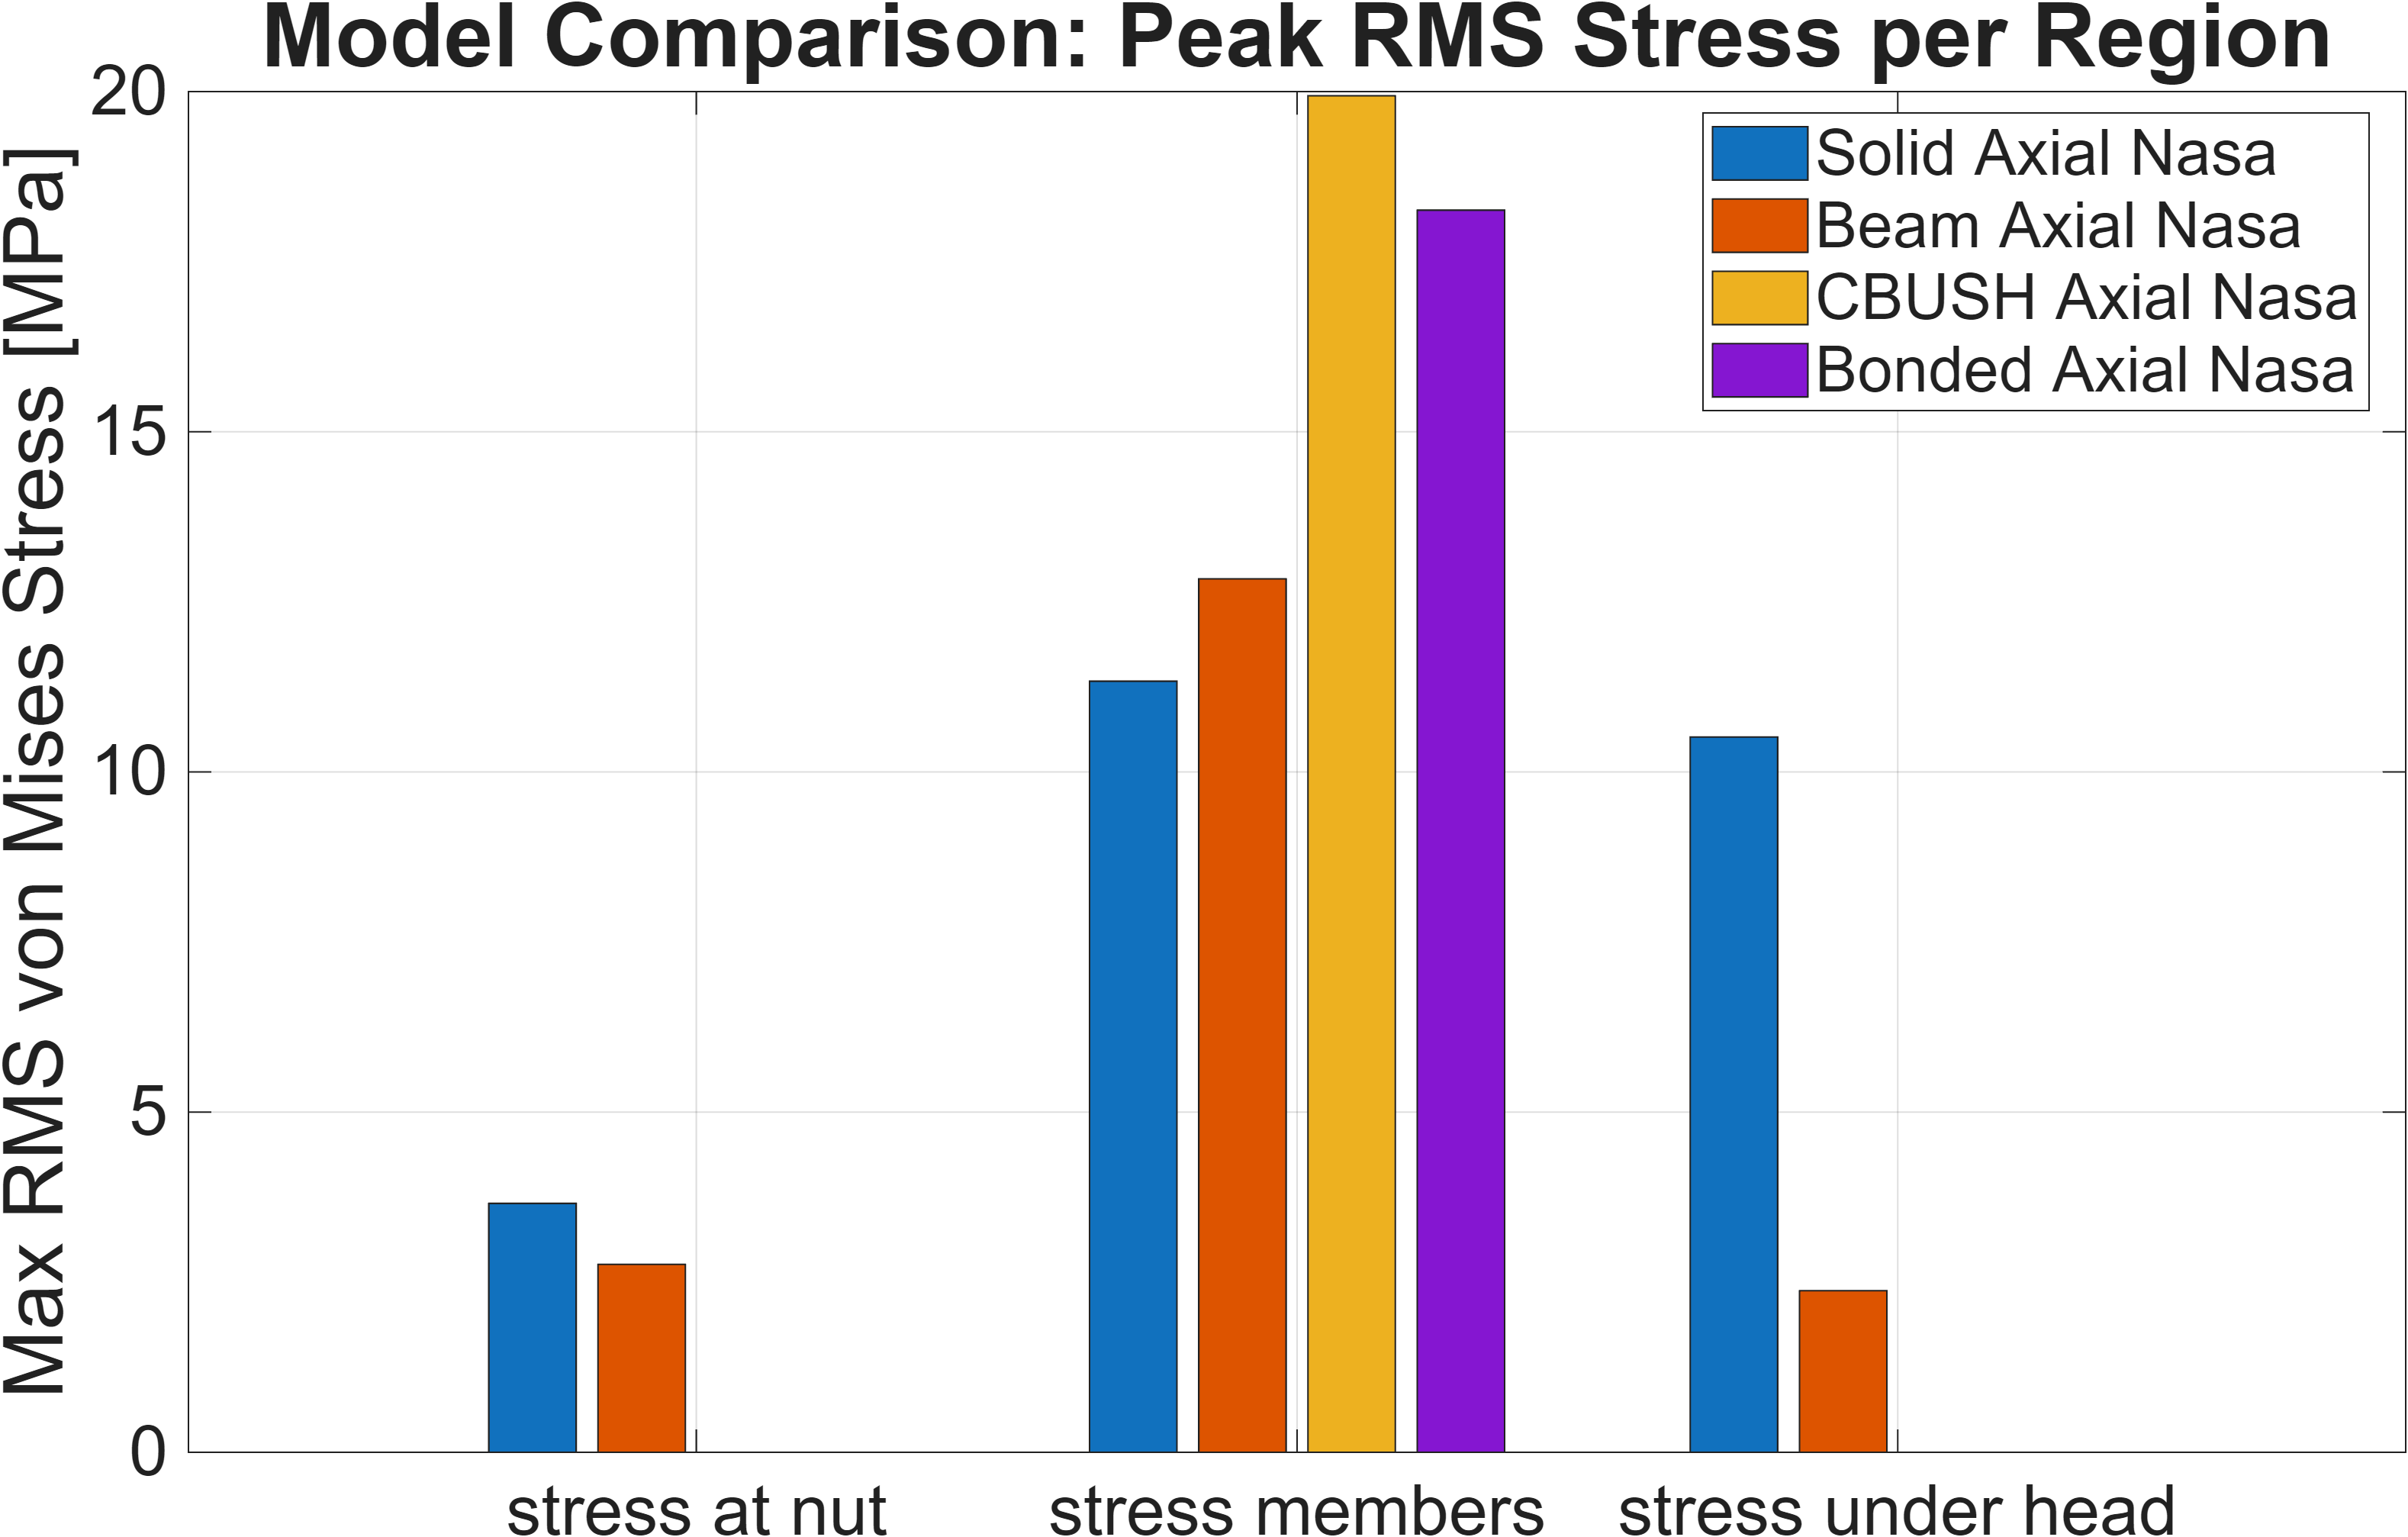
\includegraphics[width=\textwidth]{Axial Nasa/Axial Nasa_comparison_max_rms_per_region NODEWISE.png}
        \caption{Axial Loading (bending).}
        \label{fig:NASA_bending_comparison_max_rms_per_region_NODEWISE}
    \end{subfigure}
    
    \caption{Maximum \ac{RMS} von Mises stress per region and model. The same trends are visible in the corresponding T43A results, see Appendix \ref{app:T43A_figures}.}
    \label{fig:RMS_per_region}
\end{figure}

\begin{figure}[H]
    \centering
    \begin{subfigure}[b]{0.45\textwidth}
        \centering
        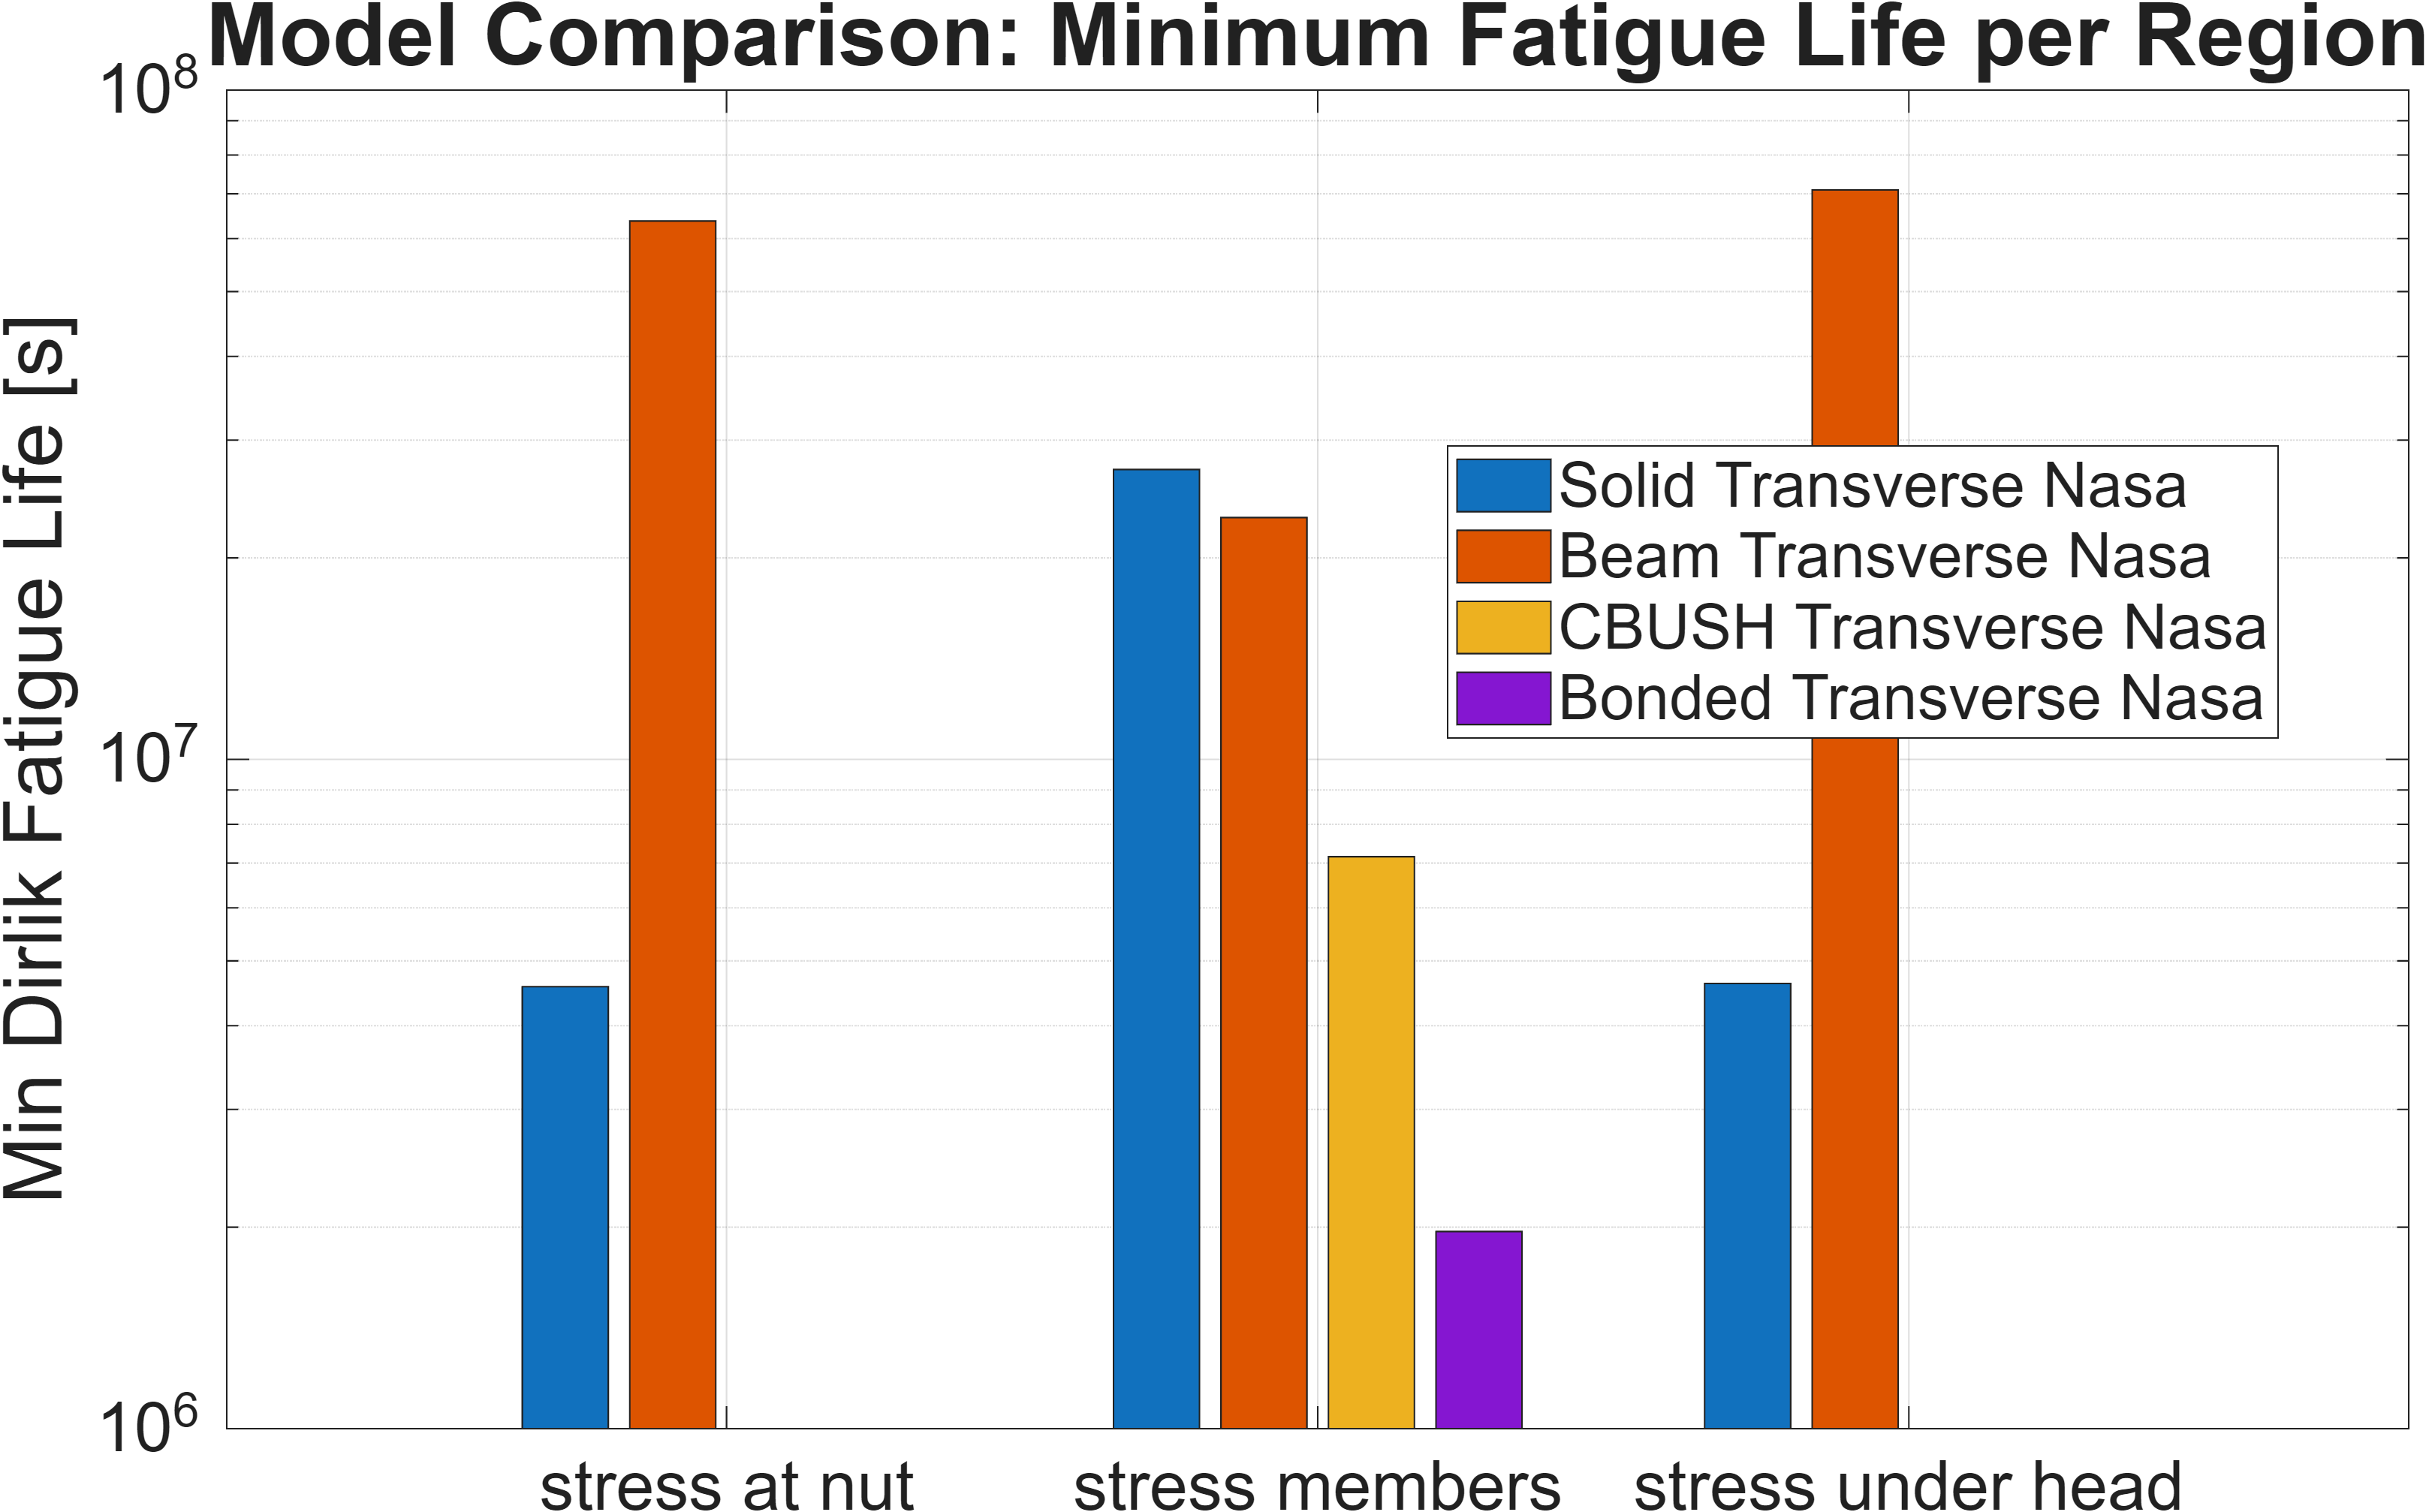
\includegraphics[width=\textwidth]{Transverse Nasa/Transverse Nasa_comparison_min_life_per_region NODEWISE.png}
        \caption{Transverse Loading (shear).}
        \label{fig:NASA_shear_comparison_min_life_per_region_NODEWISE}
    \end{subfigure}
    \begin{subfigure}[b]{0.45\textwidth}
        \centering
        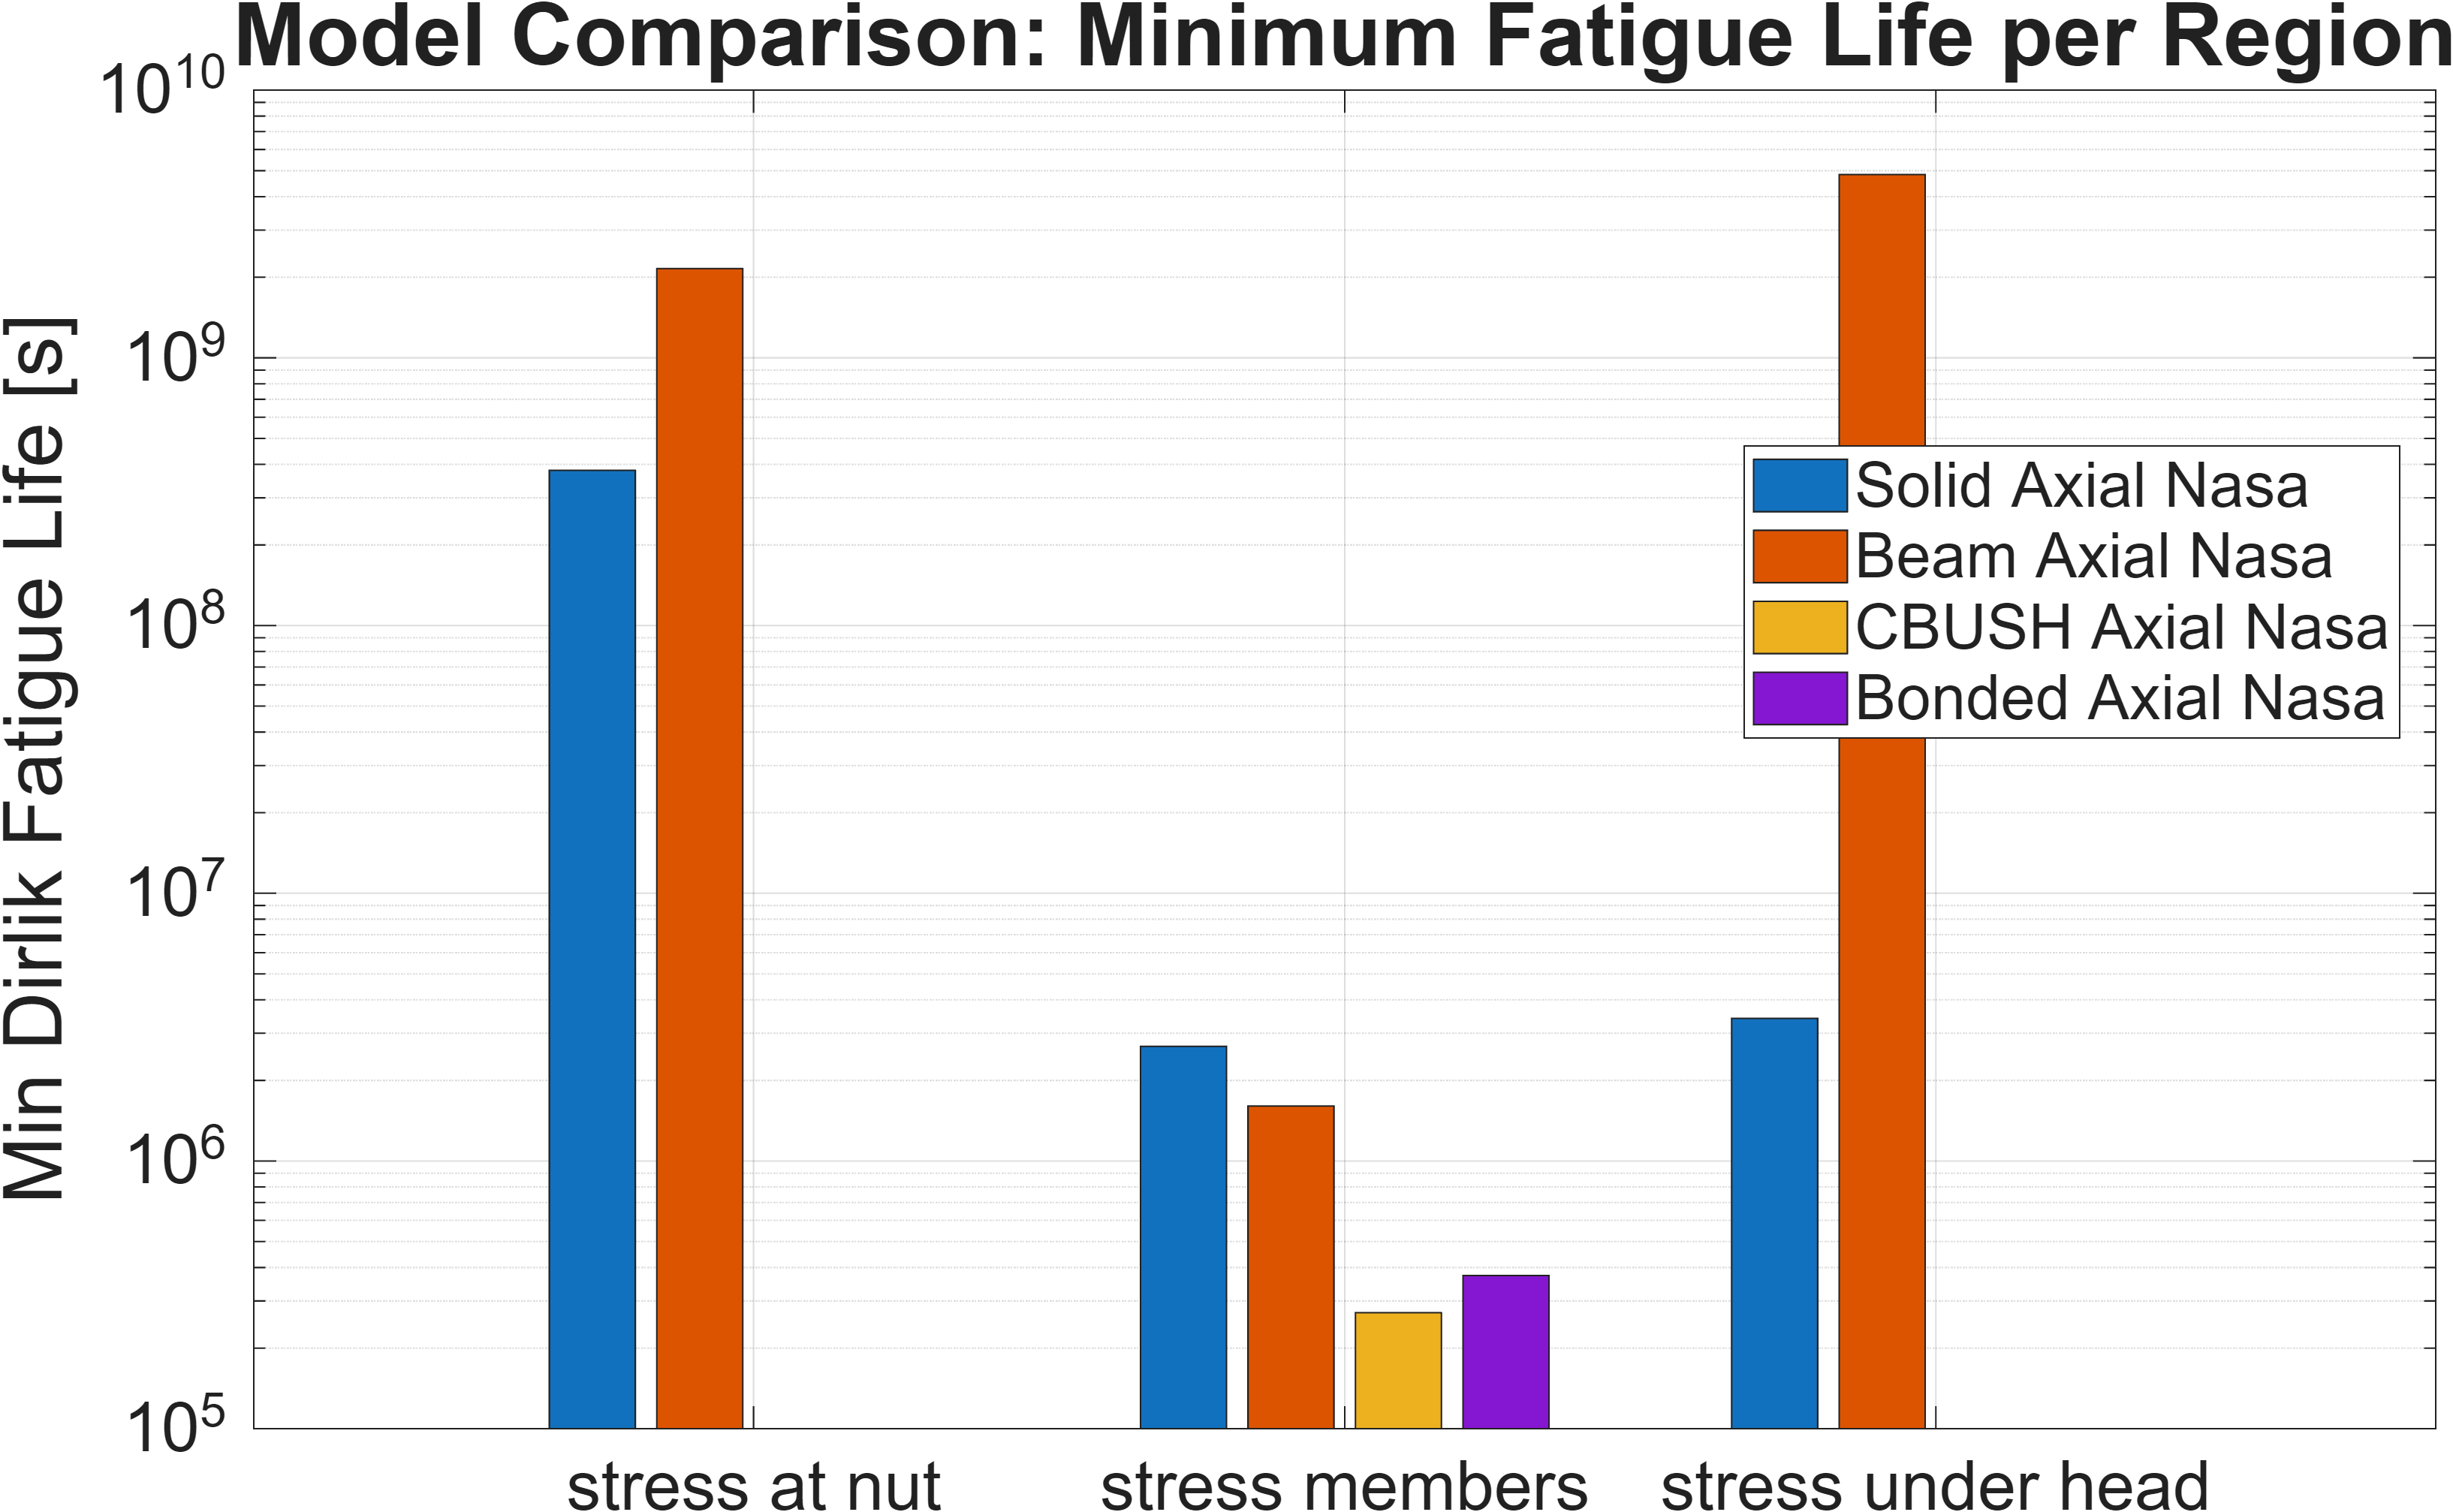
\includegraphics[width=\textwidth]{Axial Nasa/Axial Nasa_comparison_min_life_per_region NODEWISE.png}
        \caption{Axial Loading (bending).}
        \label{fig:NASA_bending_comparison_min_life_per_region_NODEWISE}
    \end{subfigure}
    
    \caption{Minimum Dirlik fatigue life per extraction region and bolt model. The bonded model predicts the shortest life in the clamped-members region, while the beam model remains closest to the solid reference. The same trends are visible in the corresponding T43A results, see Appendix \ref{app:T43A_figures}.}
    \label{fig:Life_per_region}
\end{figure}


\newpage
\subsection{Transverse Loading}
For the NASA Workmanship transverse load case, the beam model predicts a clamped-member minimum fatigue life of $2.30\times10^{7}$ s, compared with $2.71\times10^{7}$ s for the solid reference. This corresponds to a life ratio $\tfrac{T_{model}}{T_{ref}}$ of $0.848$. The corresponding maximum \ac{RMS} stress is 3.48 MPa for the beam and 3.34 MPa for the solid, giving a 4.2\% overprediction.

The CBUSH model gives a clamped-member life of $7.16\times10^{6}$ s, corresponding to $0.264$ of the solid life, with a maximum \ac{RMS} stress of 4.68 MPa.

The bonded model gives the shortest clamped-member life in this load case, $1.97\times10^{6}$ s, corresponding to $0.073$ of the solid life, with a maximum \ac{RMS} stress of 6.38 MPa.

For the local bolt regions, the beam model predicts finite but non-conservative lives relative to the solid reference in the NASA transverse case. Under the head, the beam predicts a life of $7.09\times10^{7}$ s, compared with $4.63\times10^{6}$ s for the solid, giving a life ratio of 15.34. At the nut, the beam predicts a life of $6.37\times10^{7}$ s, compared with $4.57\times10^{6}$ s for the solid, giving a life ratio of 13.93. Although the beam overpredicts the local \ac{RMS} stress in these regions, the different Goodman mean-stress treatment leads to longer predicted fatigue life than the solid reference.

\subsection{Axial Loading}

For the NASA Workmanship axial load case, the beam model predicts a clamped-member minimum fatigue life of $1.60\times10^{6}$ s, compared with $2.68\times10^{6}$ s for the solid reference. This gives a life ratio of 0.598. The maximum \ac{RMS} stress is 12.84 MPa for the beam and 11.33 MPa for the solid, corresponding to an overprediction of 13.3\%.

The CBUSH model gives the shortest clamped-member life in this load case, $2.71\times10^{5}$ s, corresponding to 0.101 of the solid reference.

The bonded model gives $3.73\times10^{5}$ s, corresponding to 0.139 of the solid reference. Unlike the transverse NASA case, the CBUSH model is slightly more severe than the bonded model for clamped-member fatigue under axial NASA loading.

In the local bolt regions, the beam model predicts much longer lives than the solid reference. Under the head, the beam predicts a life of $4.84\times10^{9}$ s, compared with $3.41\times10^{6}$ s for the solid, giving a life ratio of 1418.6. At the nut, the beam predicts a life of $2.15\times10^{9}$ s, compared with $3.80\times10^{8}$ s for the solid, giving a life ratio of 5.67. These results show that the beam model is non-conservative in predicting local bolt fatigue under the NASA axial load case. This occurs because the beam model's local \ac{RMS} stress in the under-head region is only 2.38 MPa, compared to the solids' 10.51 MPa. The beam representation cannot reproduce the local bearing stresses that occur when the bolt is loaded axially against the plate. However, it still experiences some stress due to the nodal force equilibrium. It misses the stress concentrations captured by a 3D solid-mesh solution.

An important validity boundary can therefore be drawn from these results. The beam model remains acceptable for the clamped-member response but should not be trusted for local bolt fatigue under axial-bending loading, where stress concentrations dominate.

\newpage
\section{Nodewise trends}
Figure \ref{fig:Life_VS_RMS_members}, \ref{fig:Life_VS_RMS_atNut}, and \ref{fig:Life_VS_RMS_underHead} show the nodewise relationship between \ac{RMS} and Dirlik fatigue life for each region. In all regions, the data follow an inverse power-law relationship, as expected from the SN-curve. Higher \ac{RMS} rapidly reduces predicted life.

\begin{figure}[H]
    \centering
    \begin{subfigure}[b]{0.45\textwidth}
        \centering
        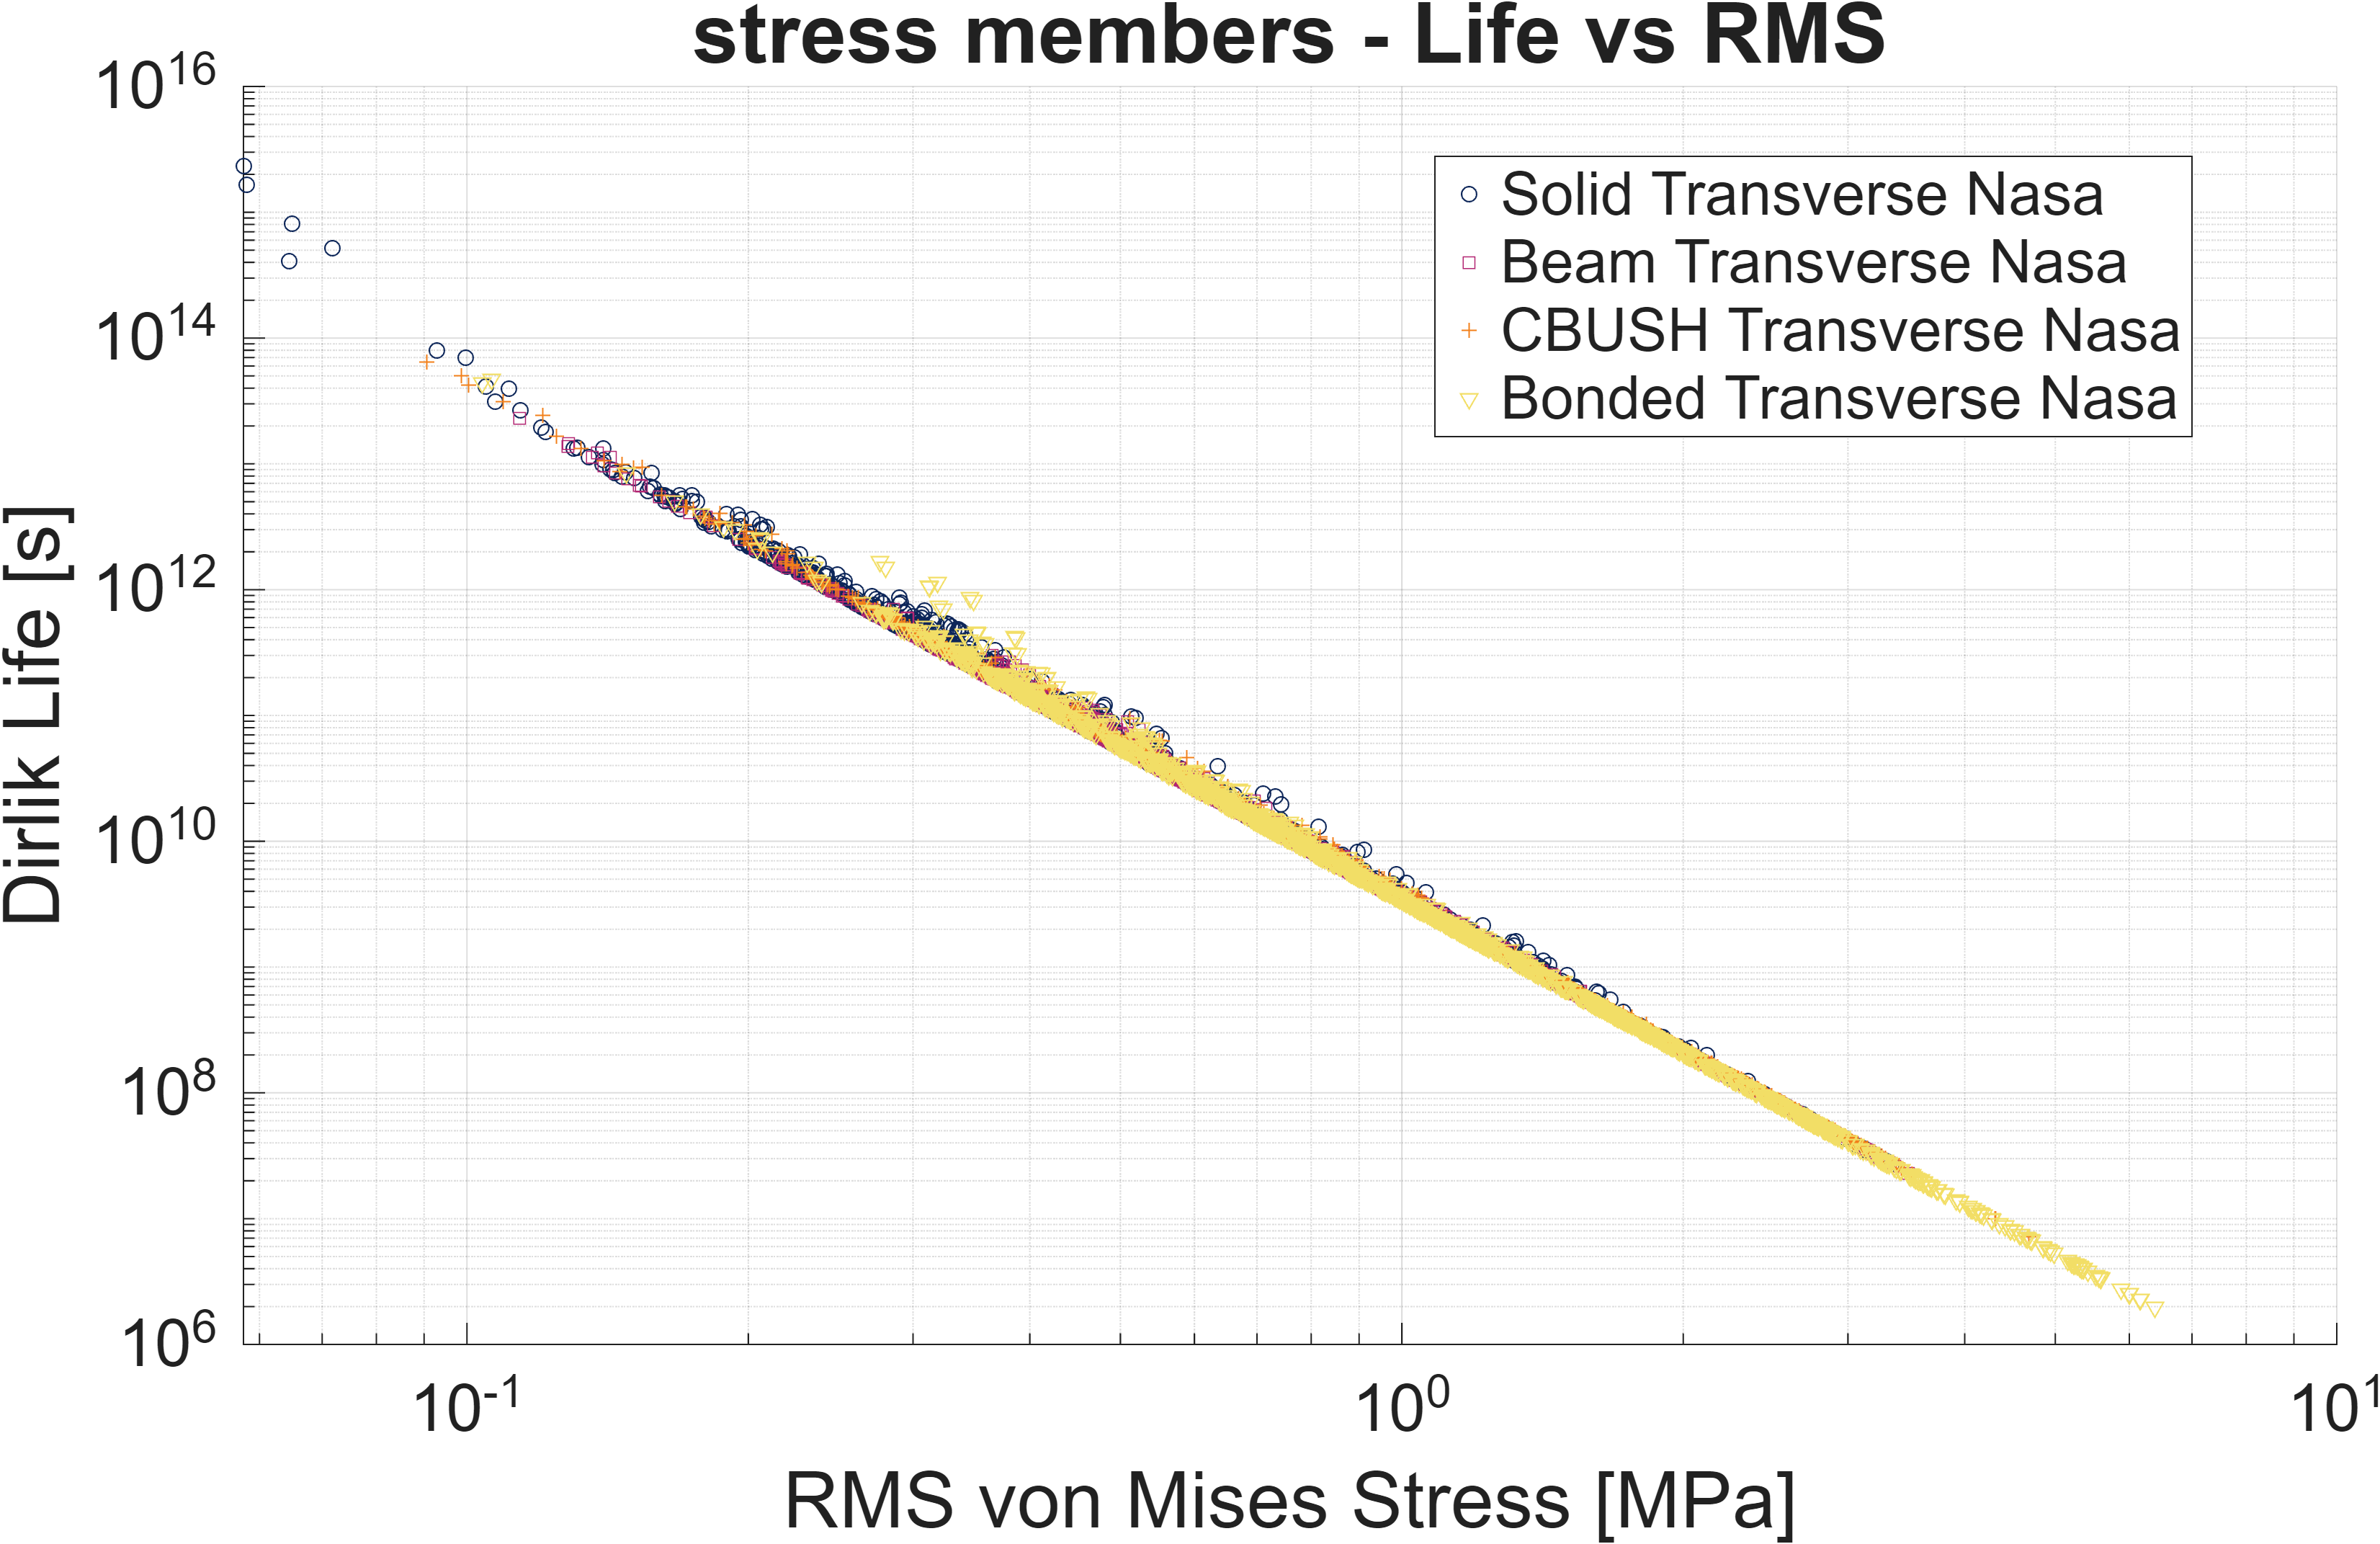
\includegraphics[width=\textwidth]{Transverse Nasa/Transverse Nasa_life_vs_rms_NODEWISE stress_members.png}
        \caption{Transverse Loading (shear).}
        \label{fig:NASA_shear_life_vs_rms_NODEWISE_stress_members}
    \end{subfigure}
    \begin{subfigure}[b]{0.45\textwidth}
        \centering
        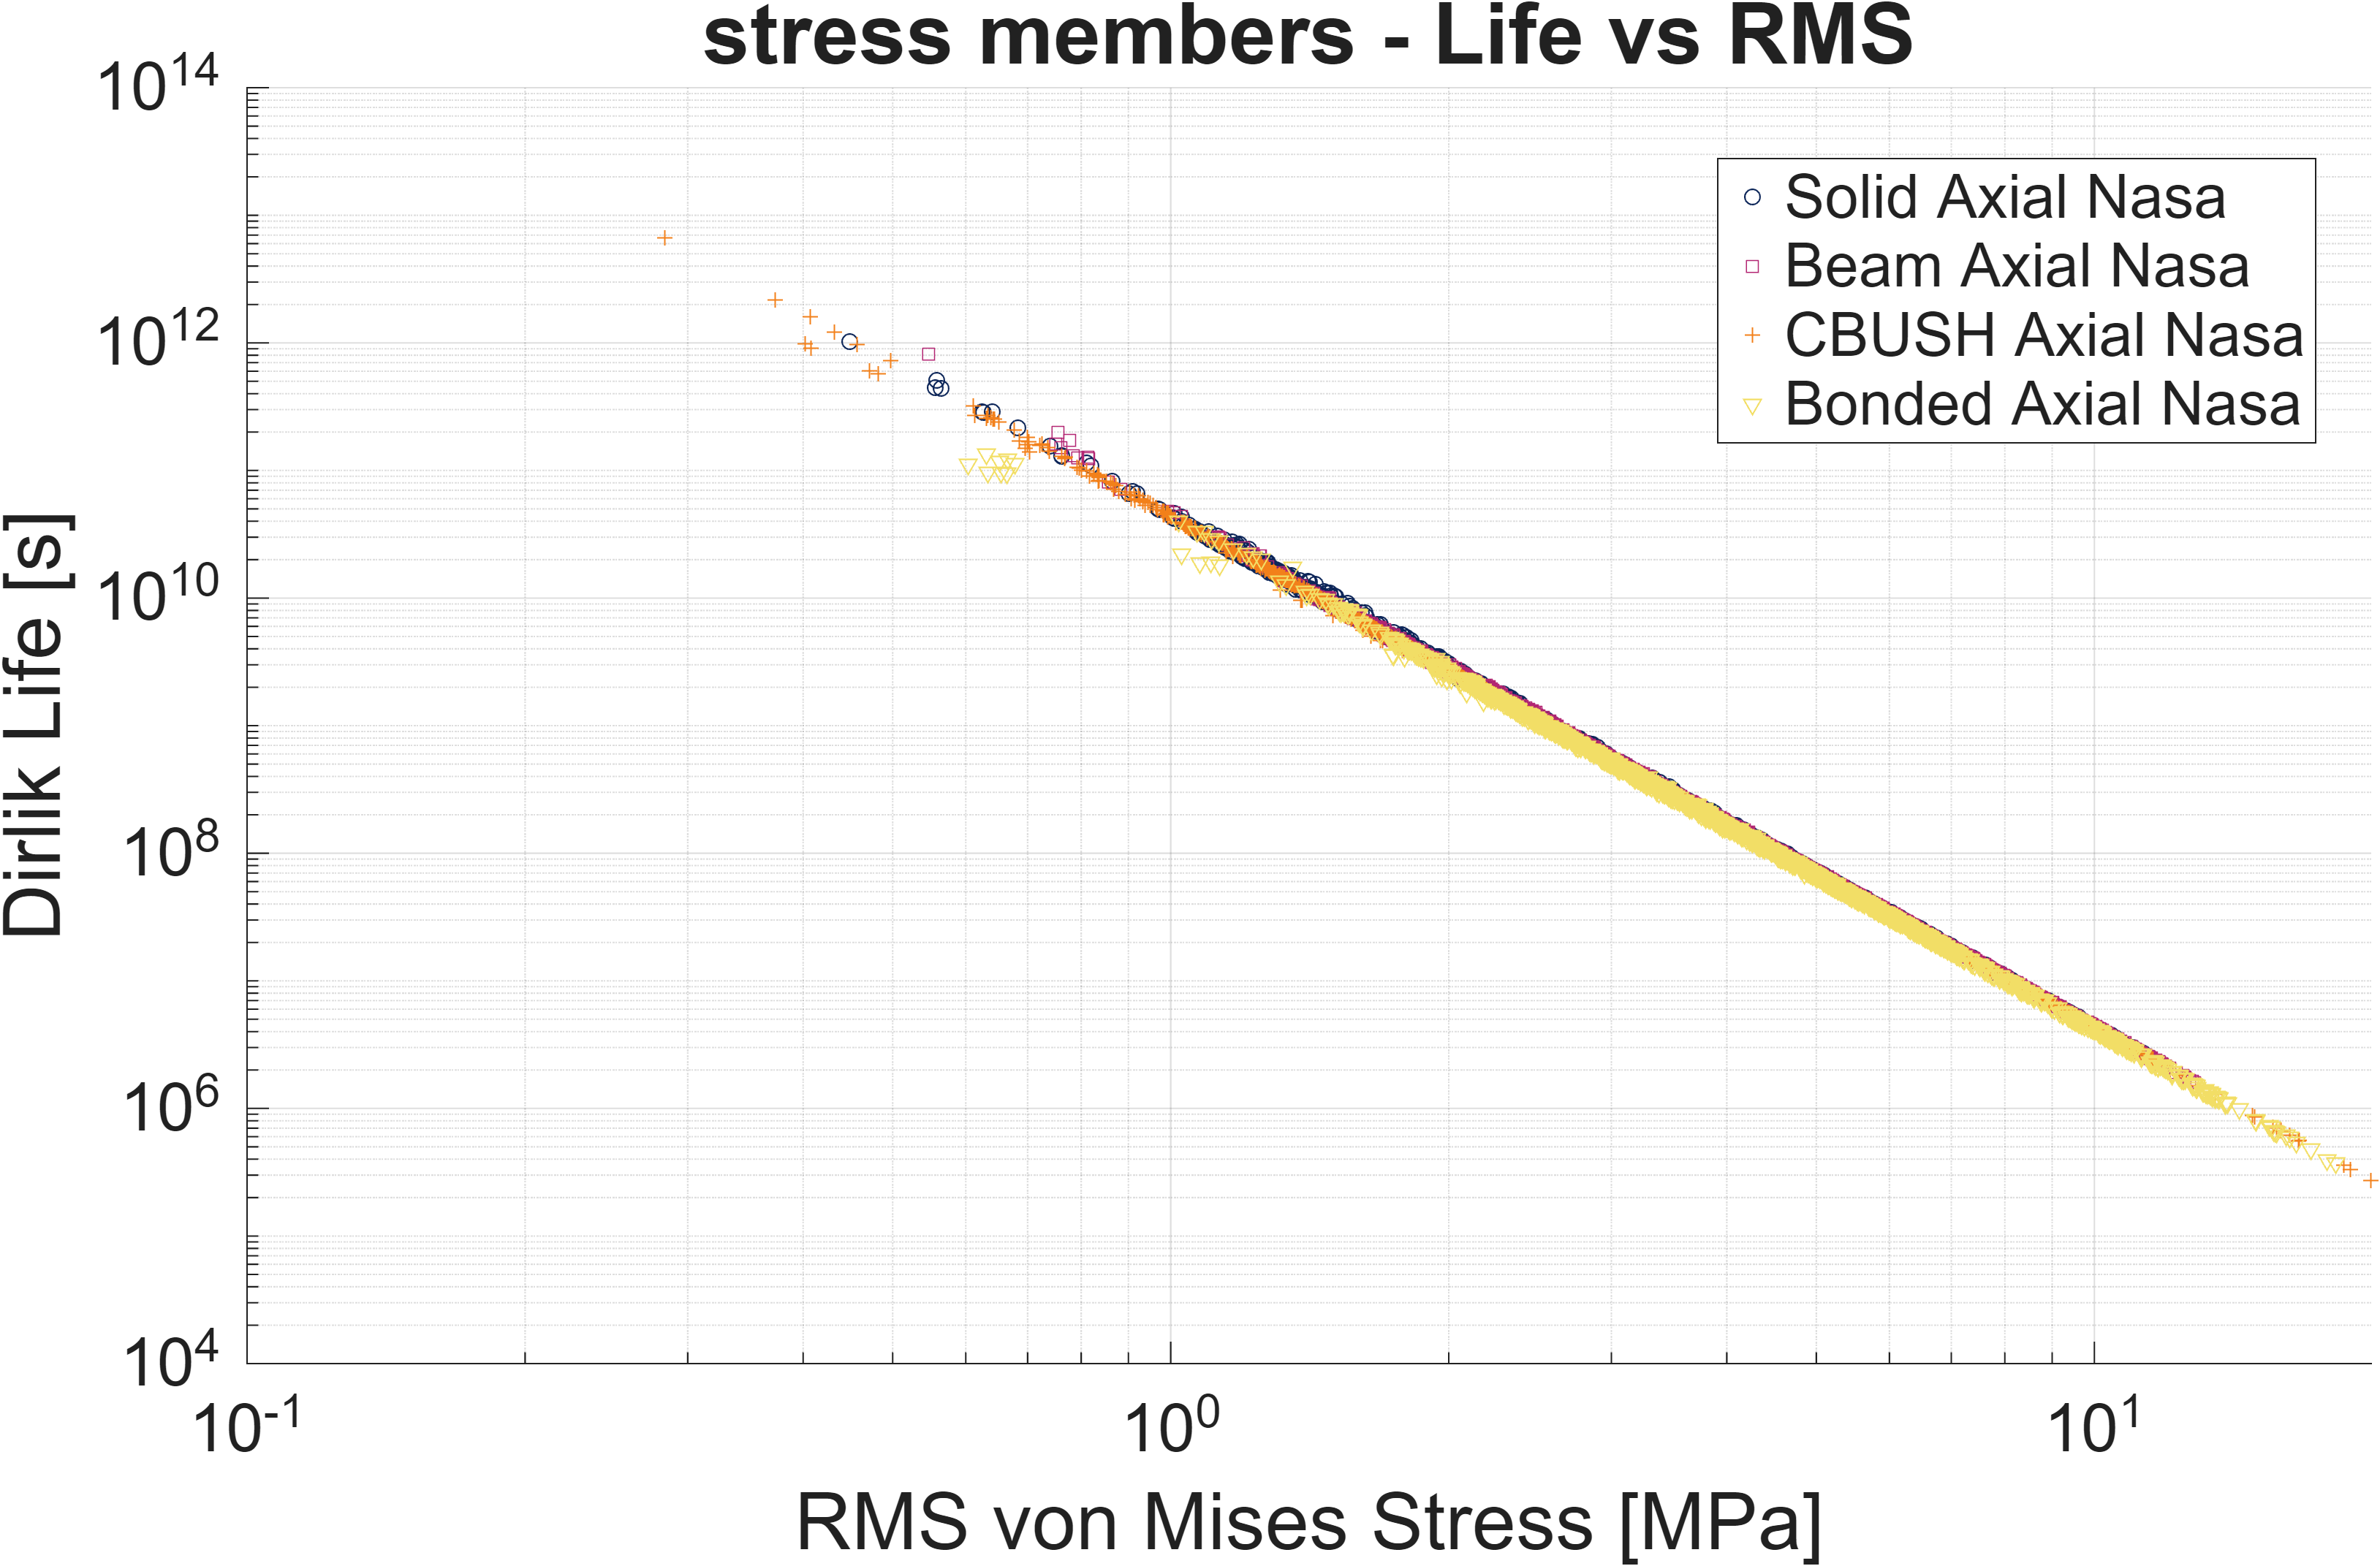
\includegraphics[width=\textwidth]{Axial Nasa/Axial Nasa_life_vs_rms_NODEWISE stress_members.png}
        \caption{Axial Loading (bending).}
        \label{fig:NASA_bending_life_vs_rms_NODEWISE_stress_members}
    \end{subfigure}
    
    \caption{Dirlik life versus \ac{RMS} stress for the clamped members. The bonded model yields the highest \ac{RMS} and, therefore, the shortest life. Excited by the NASA Workmanship profile. The same trends are visible in the corresponding T43A results, see Appendix \ref{app:T43A_figures}.}
    \label{fig:Life_VS_RMS_members}
\end{figure}

Overall, the fatigue-life comparison shows that the beam model is the closest simplified alternative to the solid reference in the clamped-member region. In contrast, the bonded model overpredicts by a large margin.

\begin{figure}[H]
    \centering
    \begin{subfigure}[b]{0.45\textwidth}
        \centering
        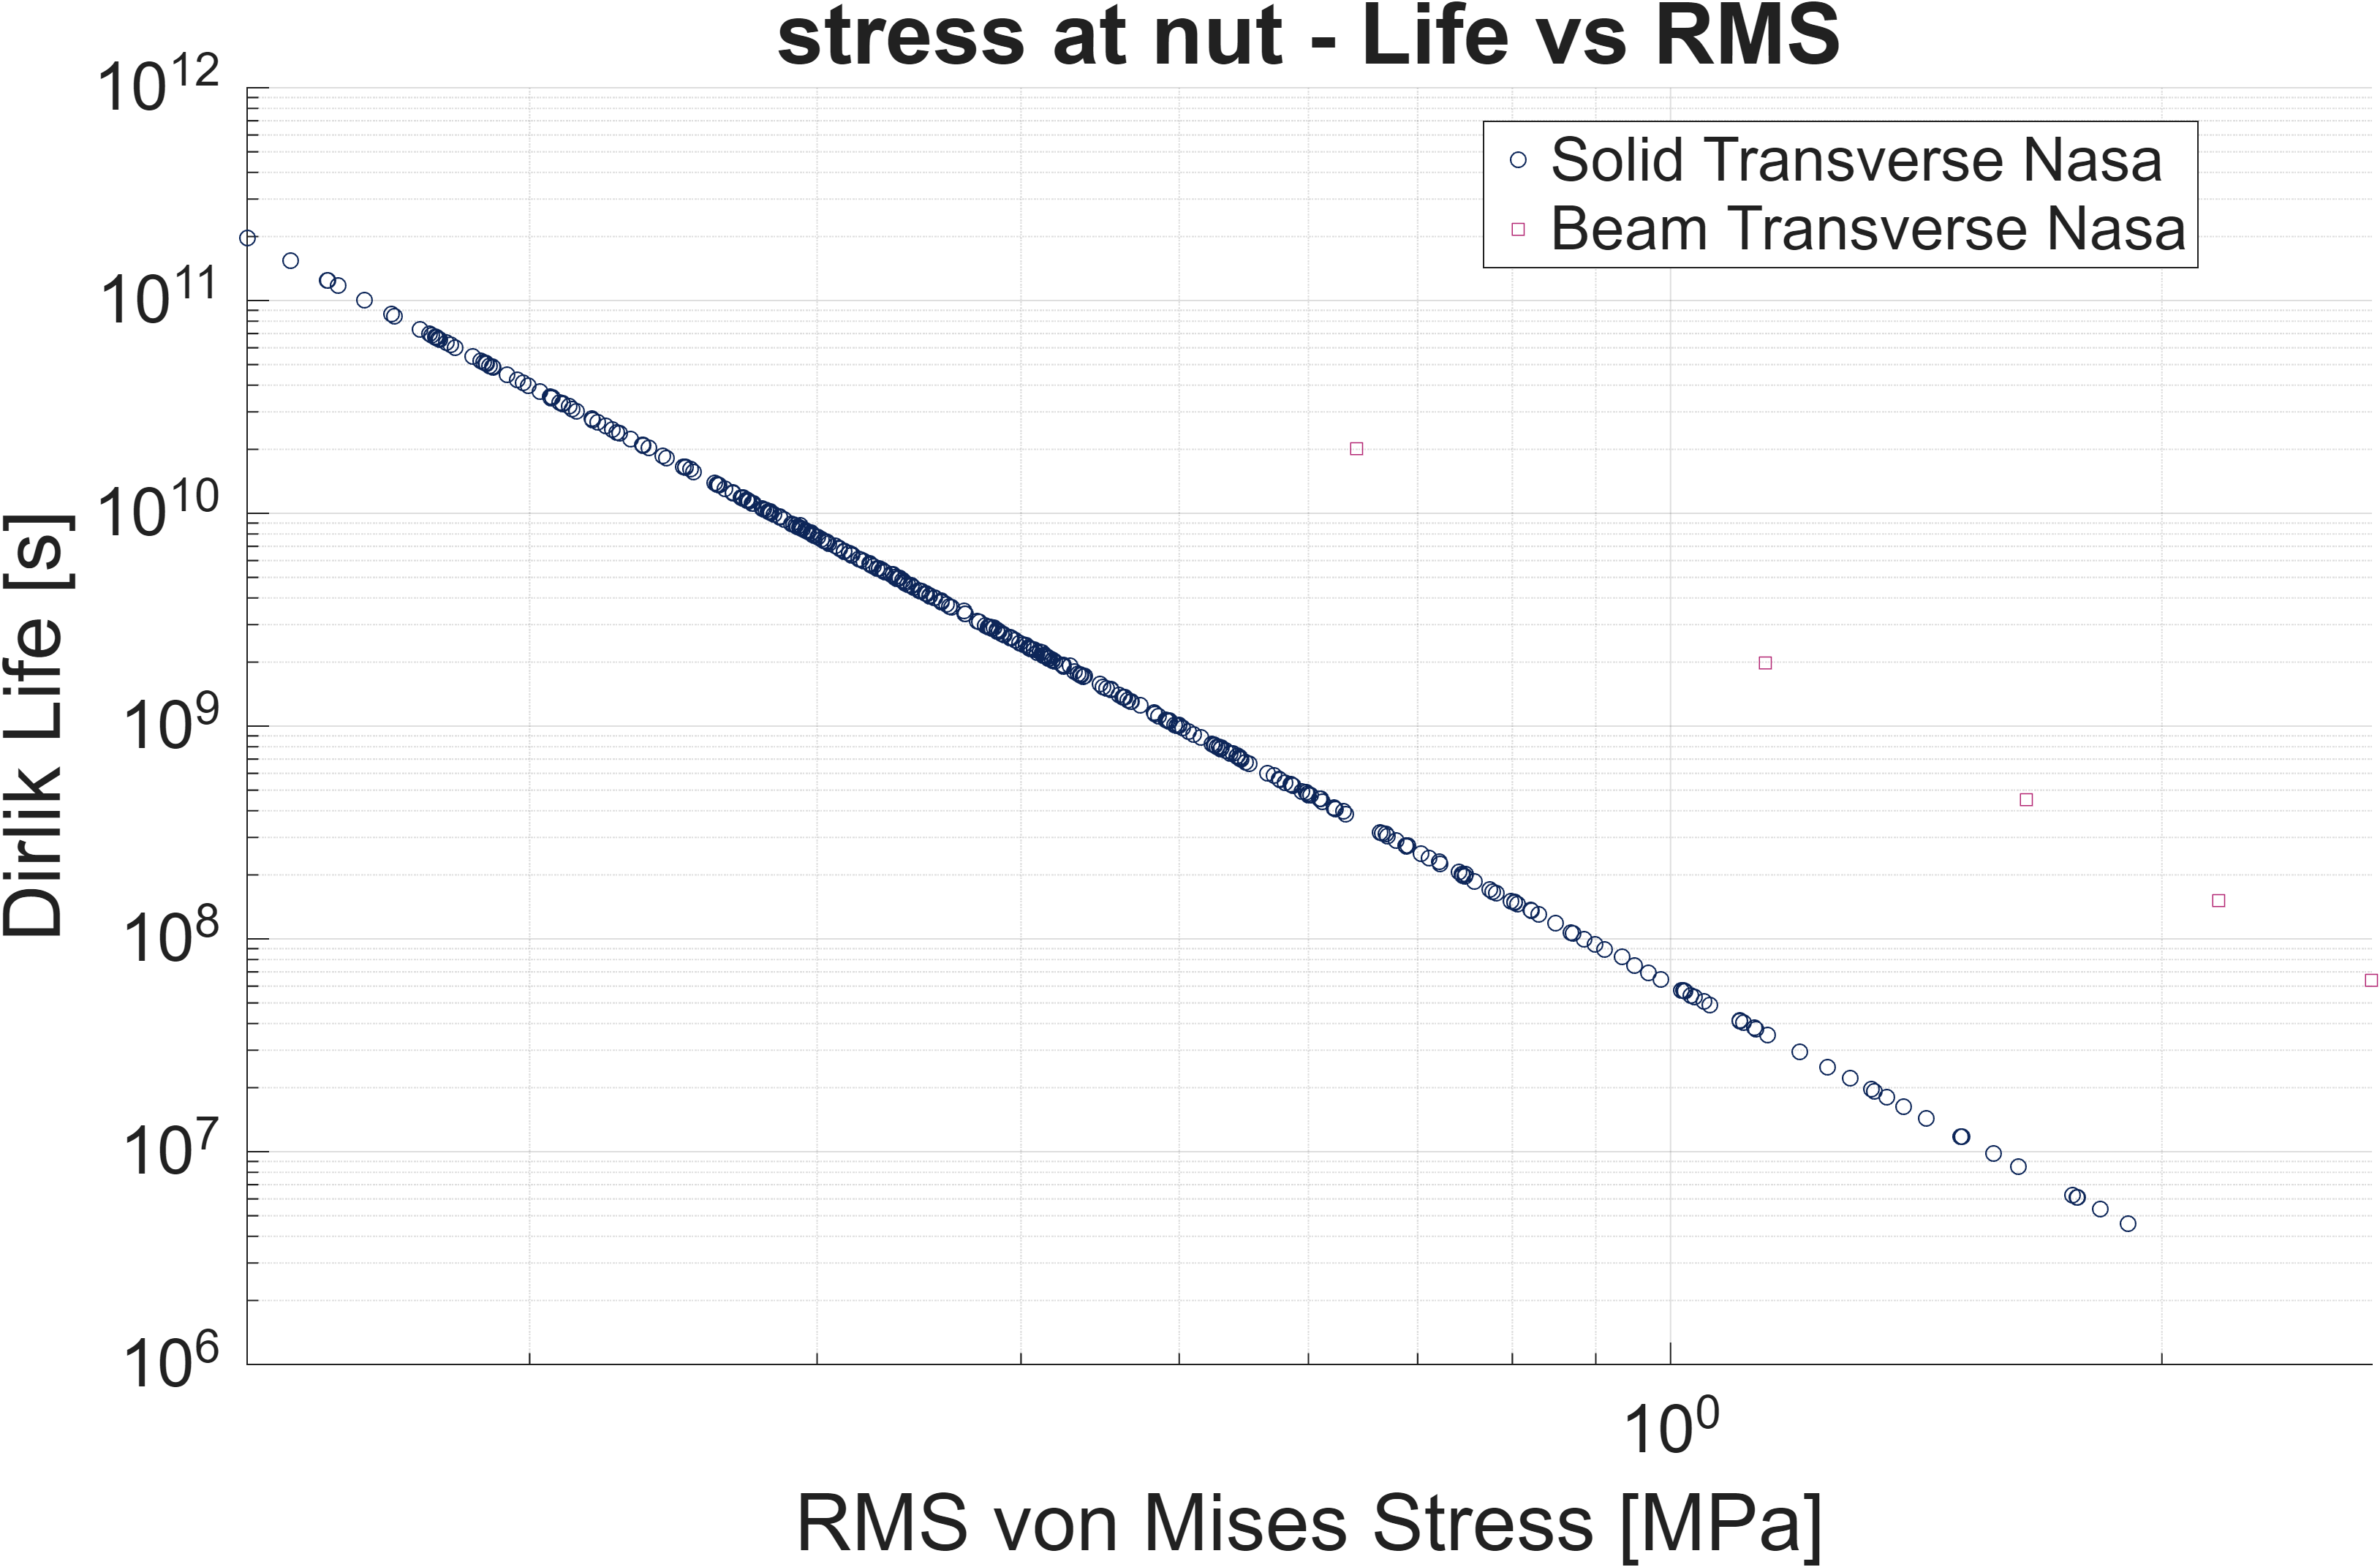
\includegraphics[width=\textwidth]{Transverse Nasa/Transverse Nasa_life_vs_rms_NODEWISE stress_at_nut.png}
        \caption{Transverse Loading (shear).}
        \label{fig:NASA_shear_life_vs_rms_NODEWISE_stress_at_nut}
    \end{subfigure}
    \begin{subfigure}[b]{0.45\textwidth}
        \centering
        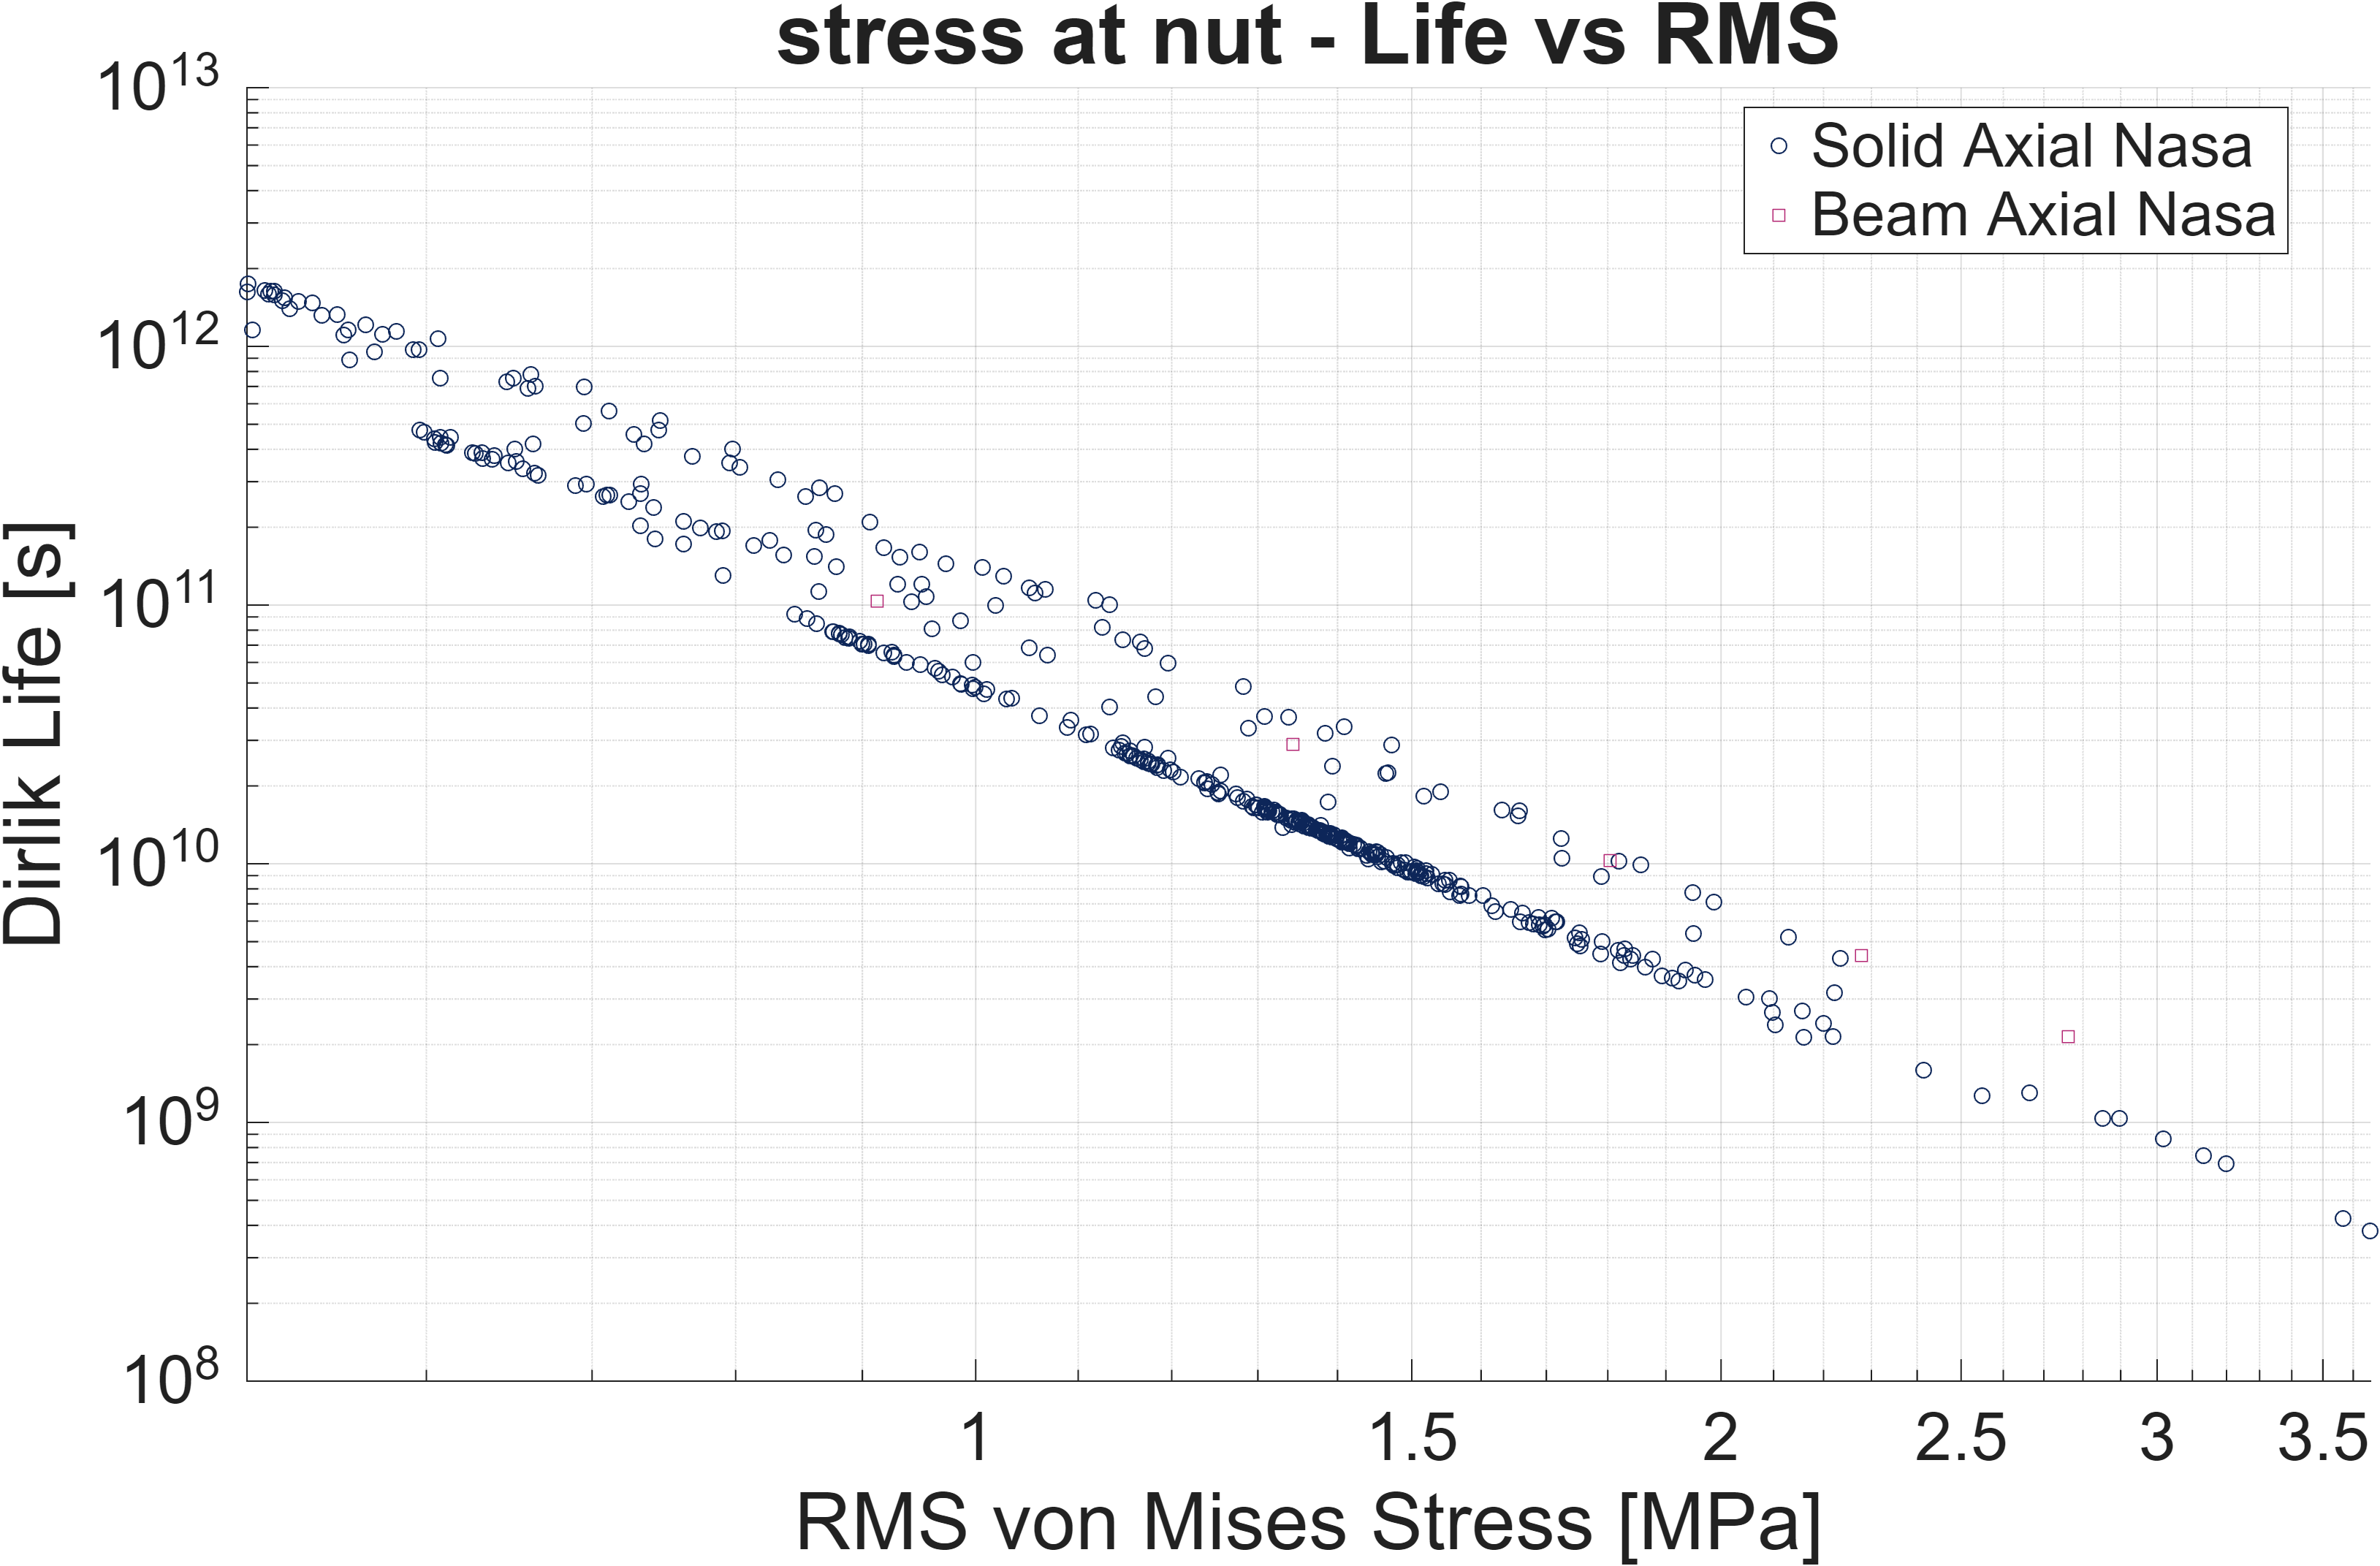
\includegraphics[width=\textwidth]{Axial Nasa/Axial Nasa_life_vs_rms_NODEWISE stress_at_nut.png}
        \caption{Axial Loading (bending).}
        \label{fig:NASA_bending_life_vs_rms_NODEWISE_stress_at_nut}
    \end{subfigure}
    
    \caption{Dirlik life versus \ac{RMS} stress for the at-nut region, solid- and beam representation only. The same trends are visible in the corresponding T43A results, see Appendix \ref{app:T43A_figures}.}
    \label{fig:Life_VS_RMS_atNut}
\end{figure}

\begin{figure}[H]
    \centering
    \begin{subfigure}[b]{0.45\textwidth}
        \centering
        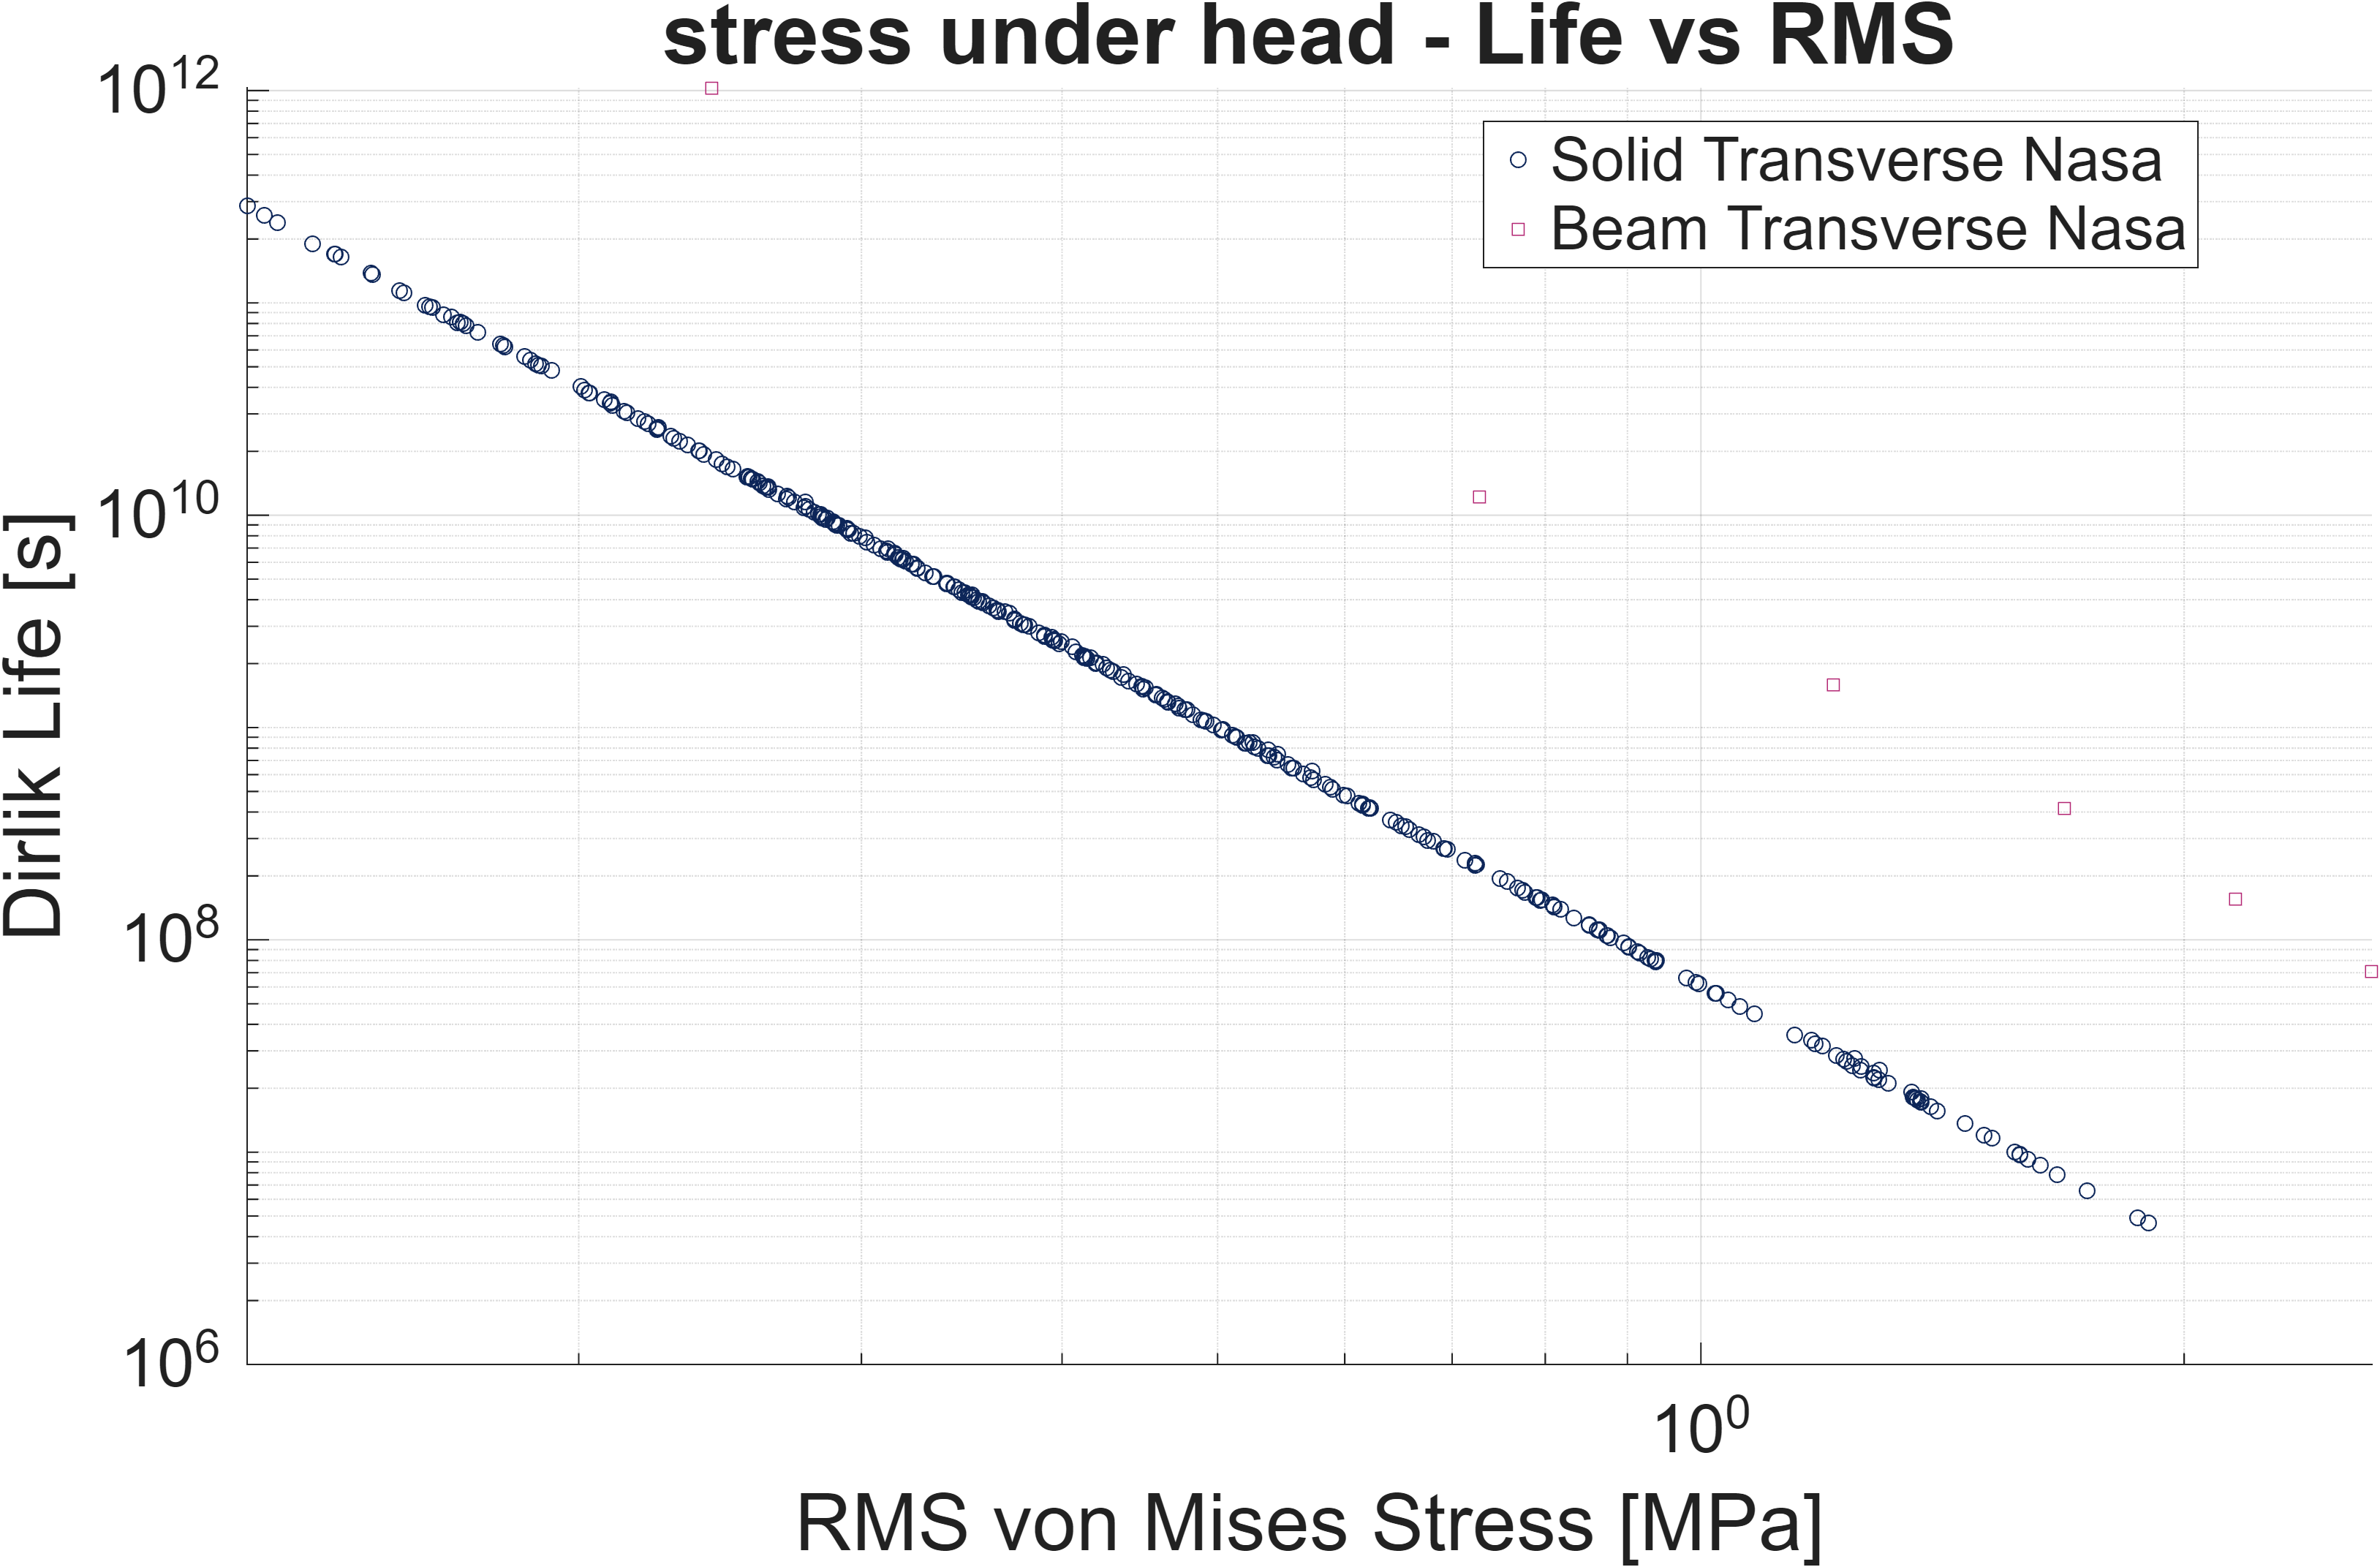
\includegraphics[width=\textwidth]{Transverse Nasa/Transverse Nasa_life_vs_rms_NODEWISE stress_under_head.png}
        \caption{Transverse Loading (shear).}
        \label{fig:NASA_shear_life_vs_rms_NODEWISE_stress_under_head}
    \end{subfigure}
    \begin{subfigure}[b]{0.45\textwidth}
        \centering
        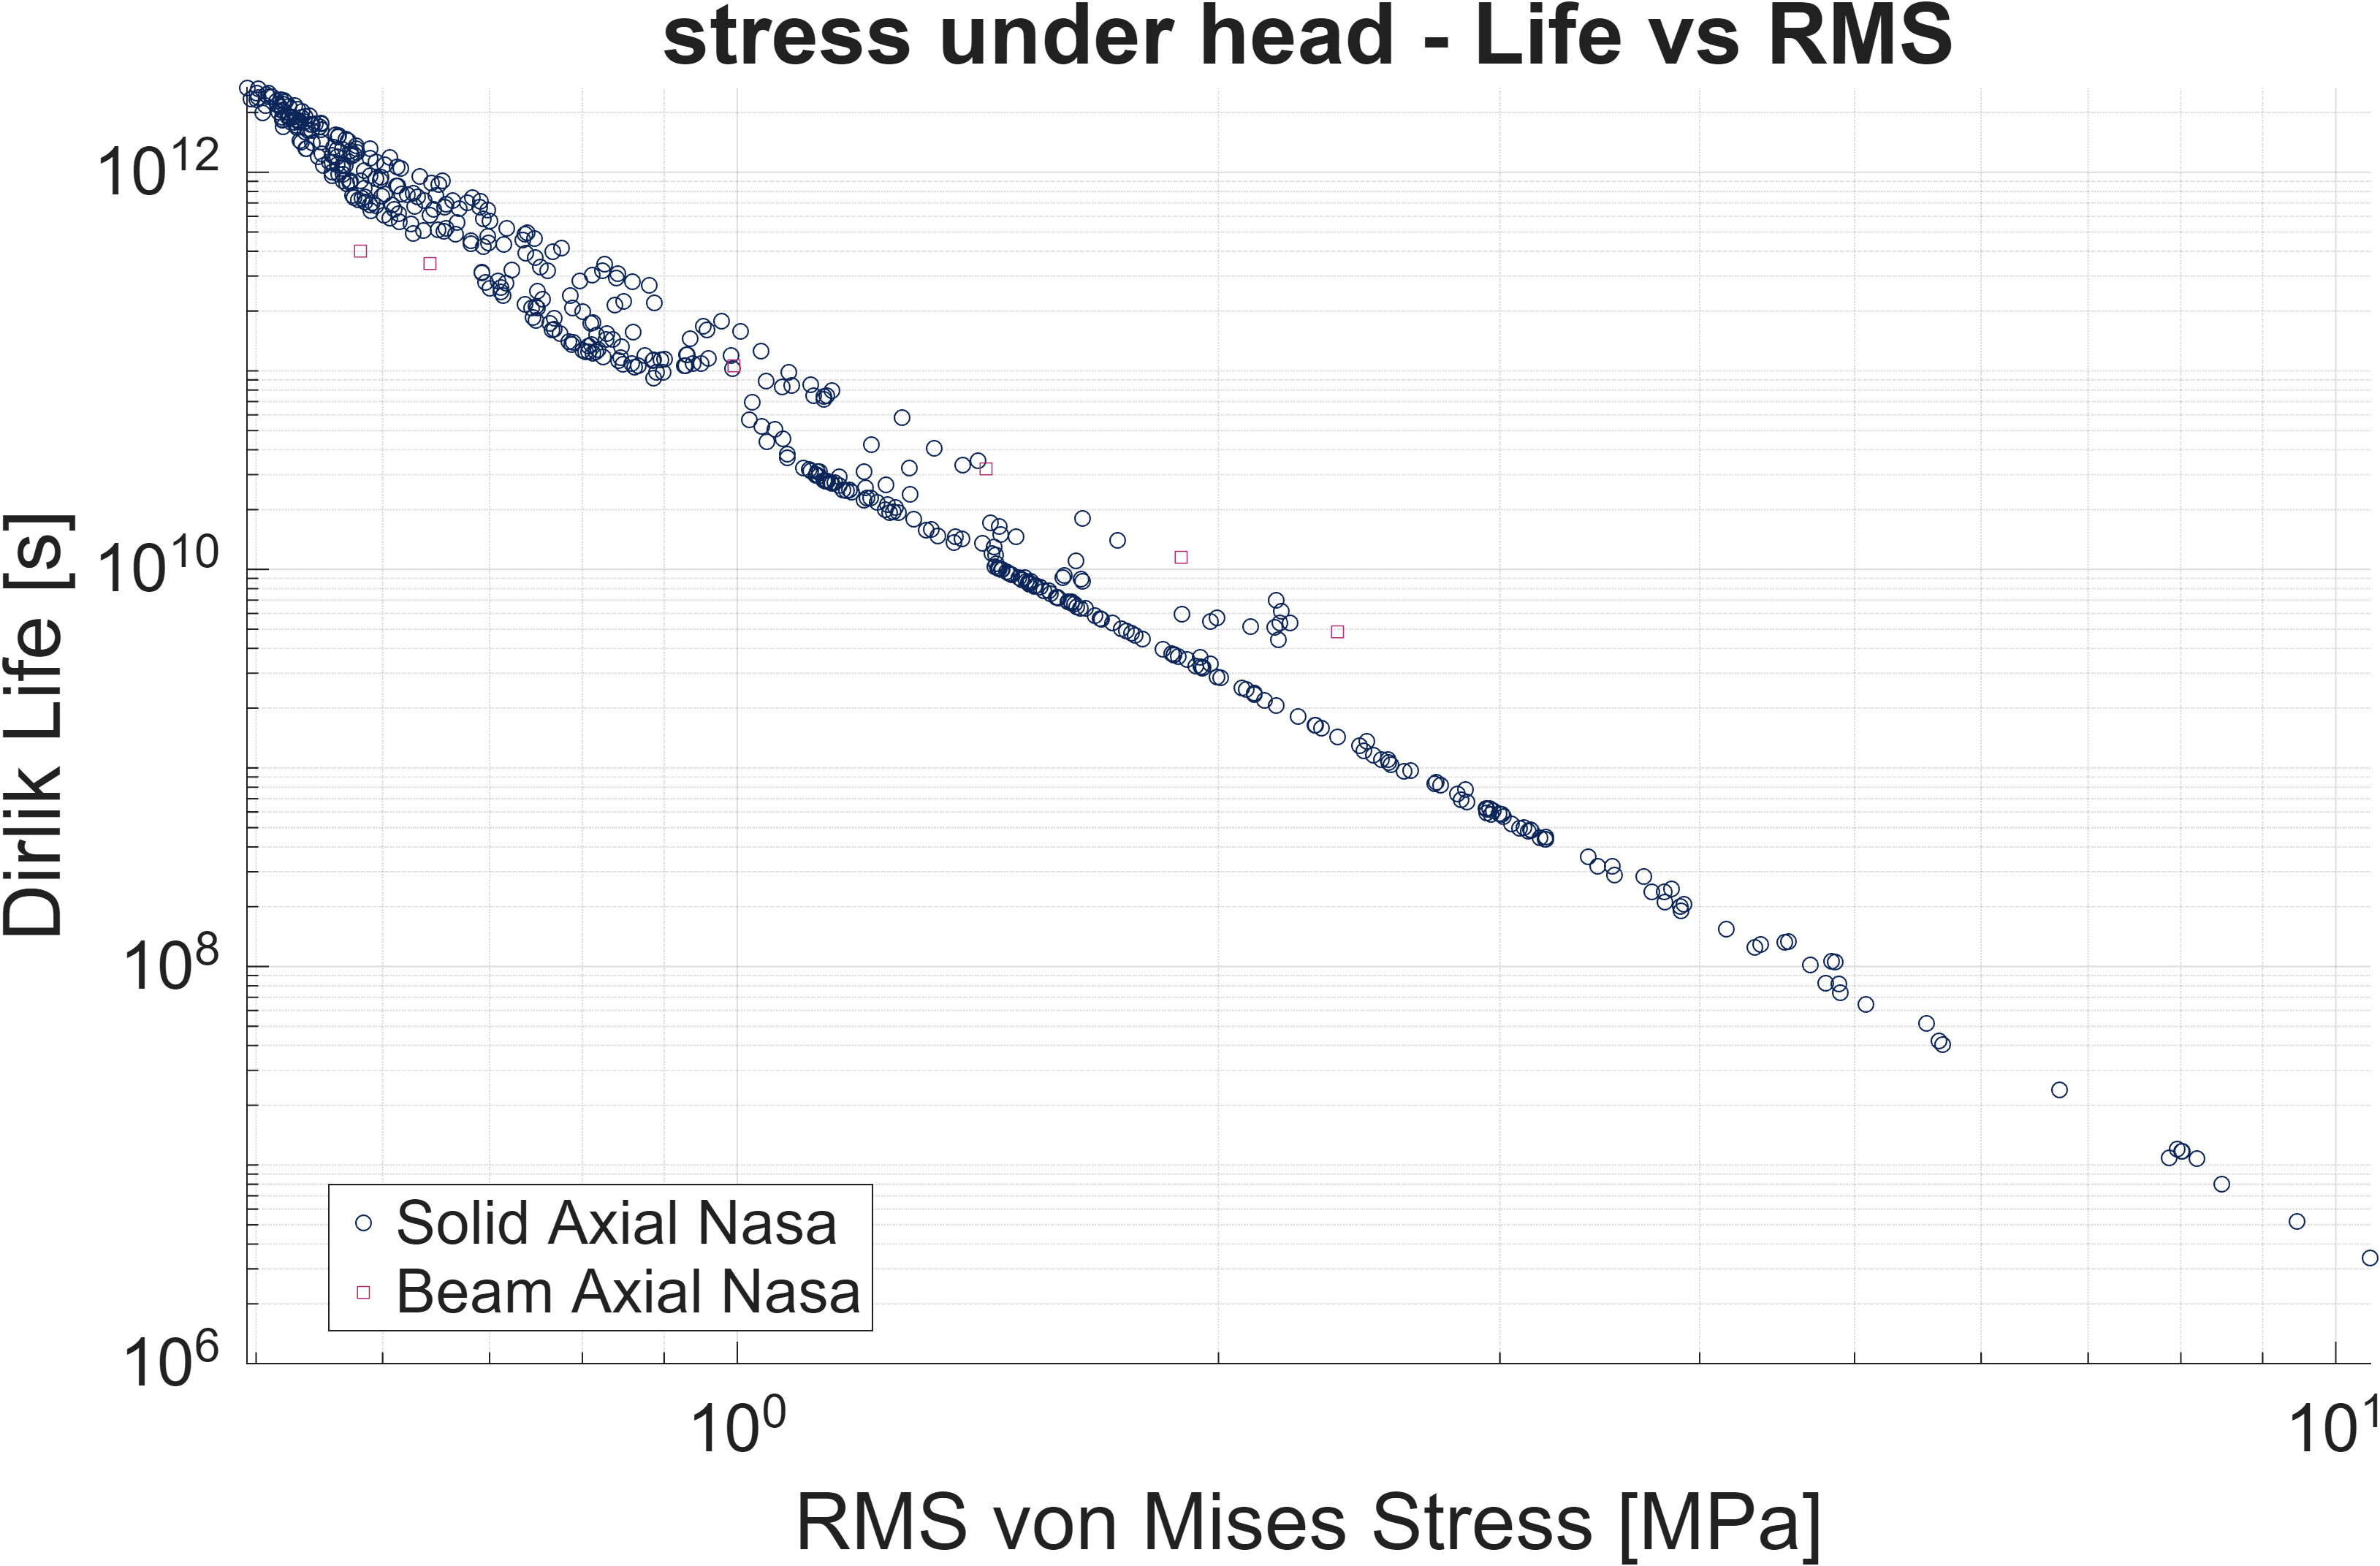
\includegraphics[width=\textwidth]{Axial Nasa/Axial Nasa_life_vs_rms_NODEWISE stress_under_head.png}
        \caption{Axial Loading (bending).}
        \label{fig:NASA_bending_life_vs_rms_NODEWISE_stress_under_head}
    \end{subfigure}
    
    \caption{Dirlik life versus \ac{RMS} stress for the under-head region, solid- and beam representation only. The same trends are visible in the corresponding T43A results, see Appendix \ref{app:T43A_figures}.}
    \label{fig:Life_VS_RMS_underHead}
\end{figure}


The \ac{RMS} von Mises stress from the random vibration analysis for the clamped-member region is, under the NASA Workmanship excitation, 3-7 MPa under transverse loading and 11-20 MPa under axial loading. Under the broader-band T43A excitation, the corresponding clamped-member ranges are roughly 0.9-2.6 MPa transverse and 15-60 MPa axially (see Appendix \ref{app:T43A_figures}). These may appear small compared to the 658 MPa nominal bolt preload stress but they are expected and consistent with the with the prestressed linear perturbation methodology: the \ac{PSD} output represents \textit{only} the dynamic stress $\sigma$ around the frozen static state $\sigma_0$. The total stress at any instant is therefore $\sigma_{tot} = \sigma_0 + \sigma$, but only $\sigma$ appears in the \ac{PSD} output. The static preload stress affects the dynamic response indirectly through the stress-stiffness matrix $S$ and through the contact state frozen during the nonlinear static step, and is accounted for separately by shifting down the SN-curve. This is also illustrated by Xiao \textit{et al.}, who reported a 3 MPa \ac{RMS} dynamic stress at a pipeline location carrying 45 MPa of static stress, supporting that the static and dynamic stress contributions can differ by more than an order of magnitude even at the same node \cite{48}.

\section{Steinberg vs Dirlik fatigue life}

The previous section compared the models using Dirlik life as the primary fatigue metric. However, the choice of spectral fatigue method can also affect the predicted life. To evaluate if the conclusions depend strongly on the selected fatigue formulation, the Dirlik and Steinberg life predictions are compared node by node in the three regions.

Figure \ref{fig:SteinbergDirlik_members}, \ref{fig:SteinbergDirlik_underHead}, and  \ref{fig:SteinbergDirlik_atNut} compare the Steinberg three-band and the Dirlik fatigue life estimates per node.
The dashed diagonal corresponds to perfect agreement between the two methods. For the most critical nodes, that is, the nodes with the shortest predicted lives, the points lie close to the 1:1 line.

In the clamped-members region (Figure \ref{fig:SteinbergDirlik_members}), the Steinberg and Dirlik estimates show strong agreement for the critical (short-life) nodes across all four models. At longer lifespans, corresponding to lower-stress nodes, the Steinberg method underpredicts slightly relative to Dirlik, leading to a conservative bias. The same trend is observed in the bolt regions (Figure \ref{fig:SteinbergDirlik_underHead} and \ref{fig:SteinbergDirlik_atNut}).

\begin{figure}[H]
    \centering
    \begin{subfigure}[b]{0.45\textwidth}
        \centering
        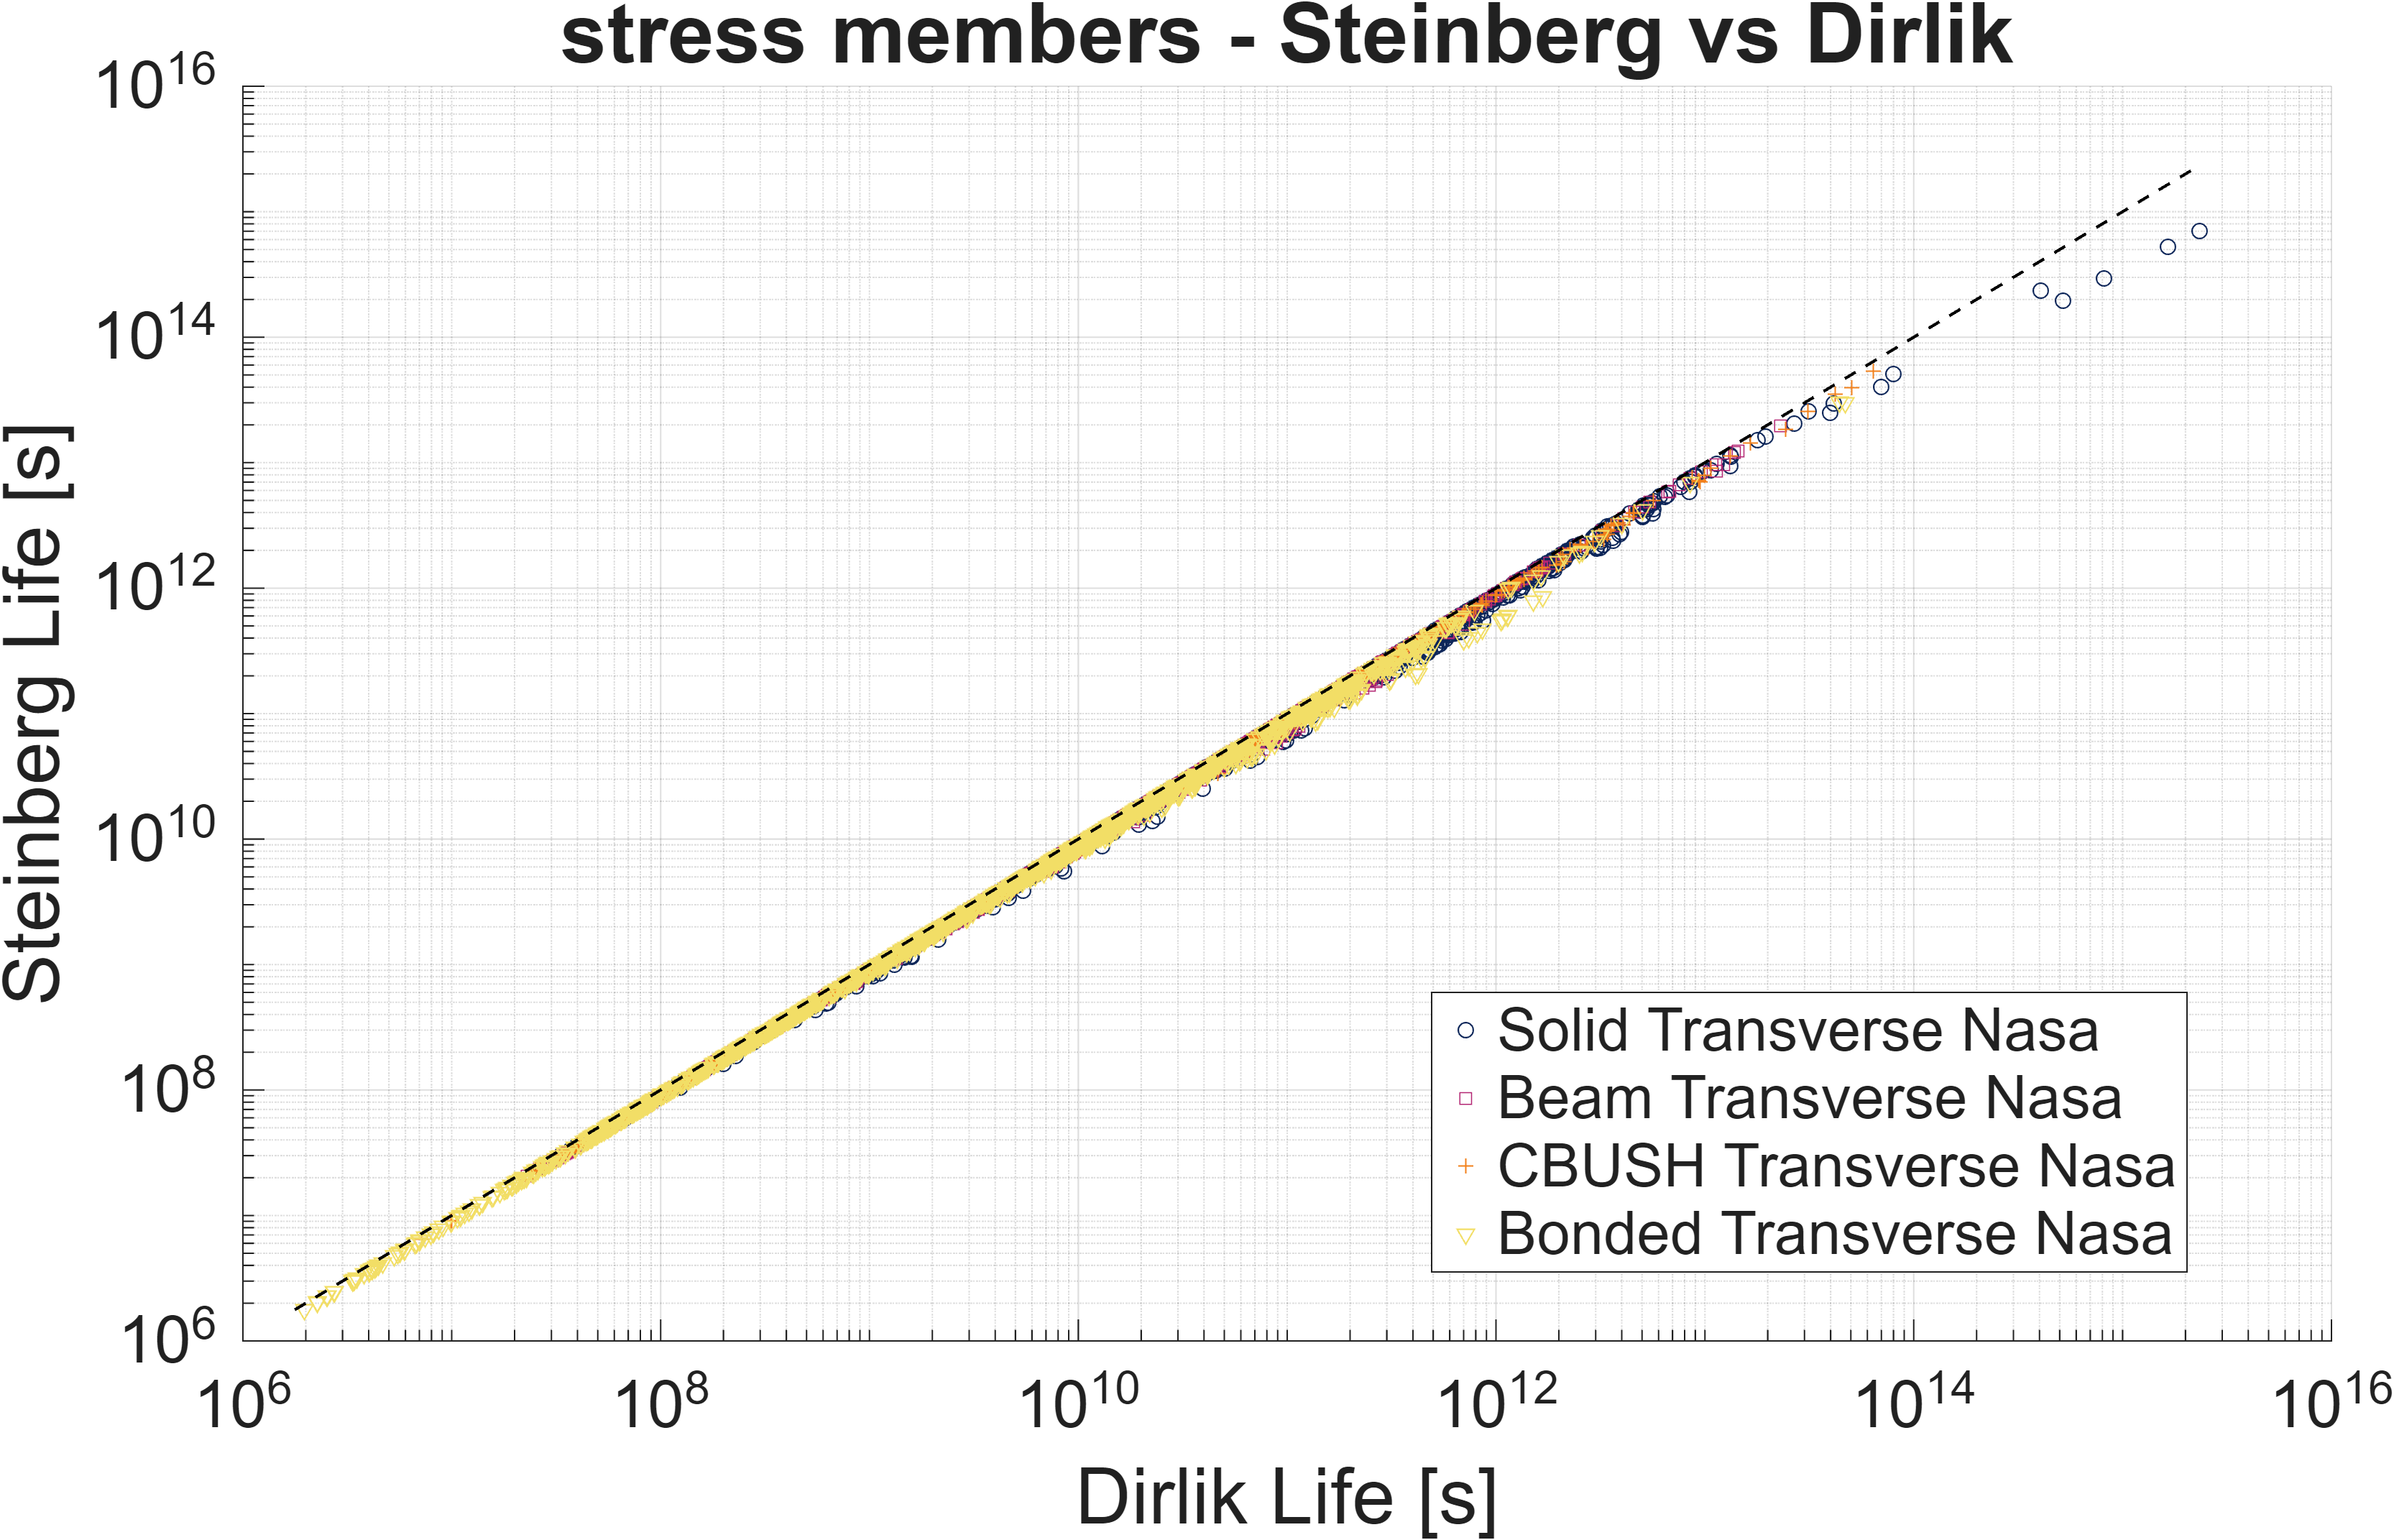
\includegraphics[width=\textwidth]{Transverse Nasa/Transverse Nasa_steinberg_vs_dirlik_NODEWISE stress_members.png}
        \caption{Transverse Loading (shear).}
        \label{fig:NASA_shear_steinberg_vs_dirlik_NODEWISE_stress_members}
    \end{subfigure}
    \begin{subfigure}[b]{0.45\textwidth}
        \centering
        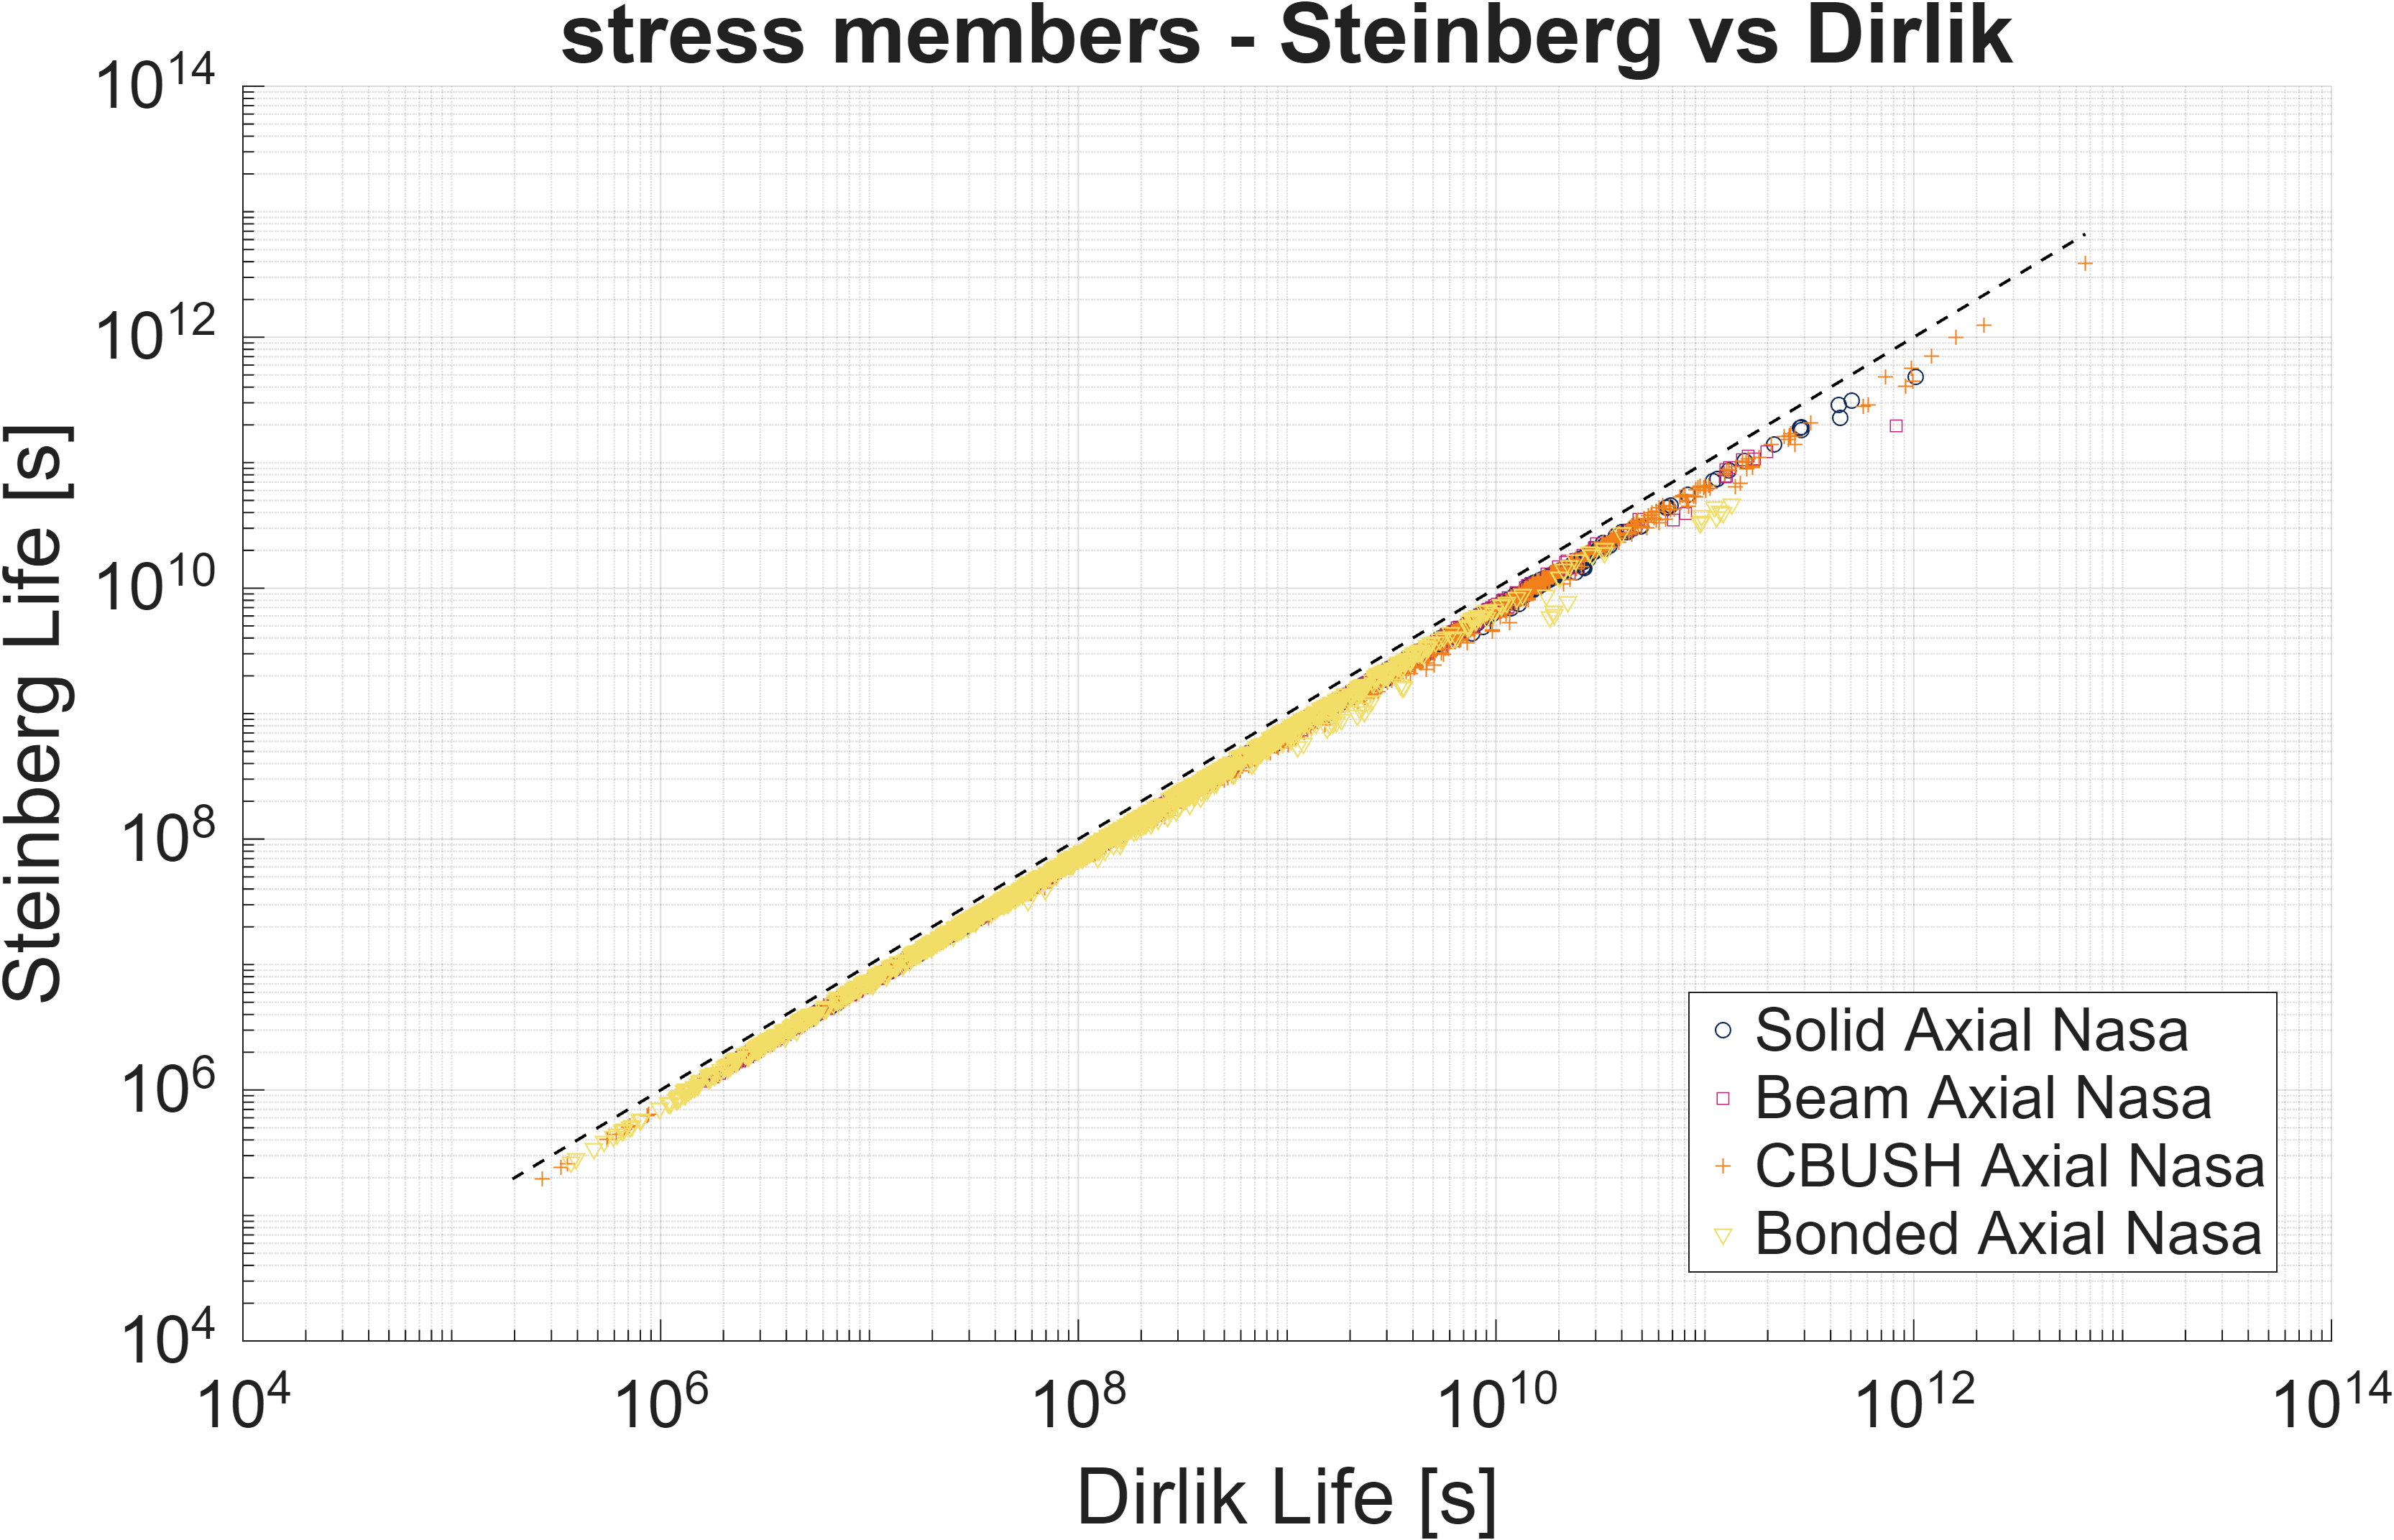
\includegraphics[width=\textwidth]{Axial Nasa/Axial Nasa_steinberg_vs_dirlik_NODEWISE stress_members.png}
        \caption{Axial Loading (bending).}
        \label{fig:NASA_bending_steinberg_vs_dirlik_NODEWISE_stress_members}
    \end{subfigure}
    
    \caption{Steinberg versus Dirlik fatigue life for the clamped members region. The same trends are visible in the corresponding T43A results, see Appendix \ref{app:T43A_figures}.}
    \label{fig:SteinbergDirlik_members}
\end{figure}

\begin{figure}[H]
    \centering
    \begin{subfigure}[b]{0.45\textwidth}
        \centering
        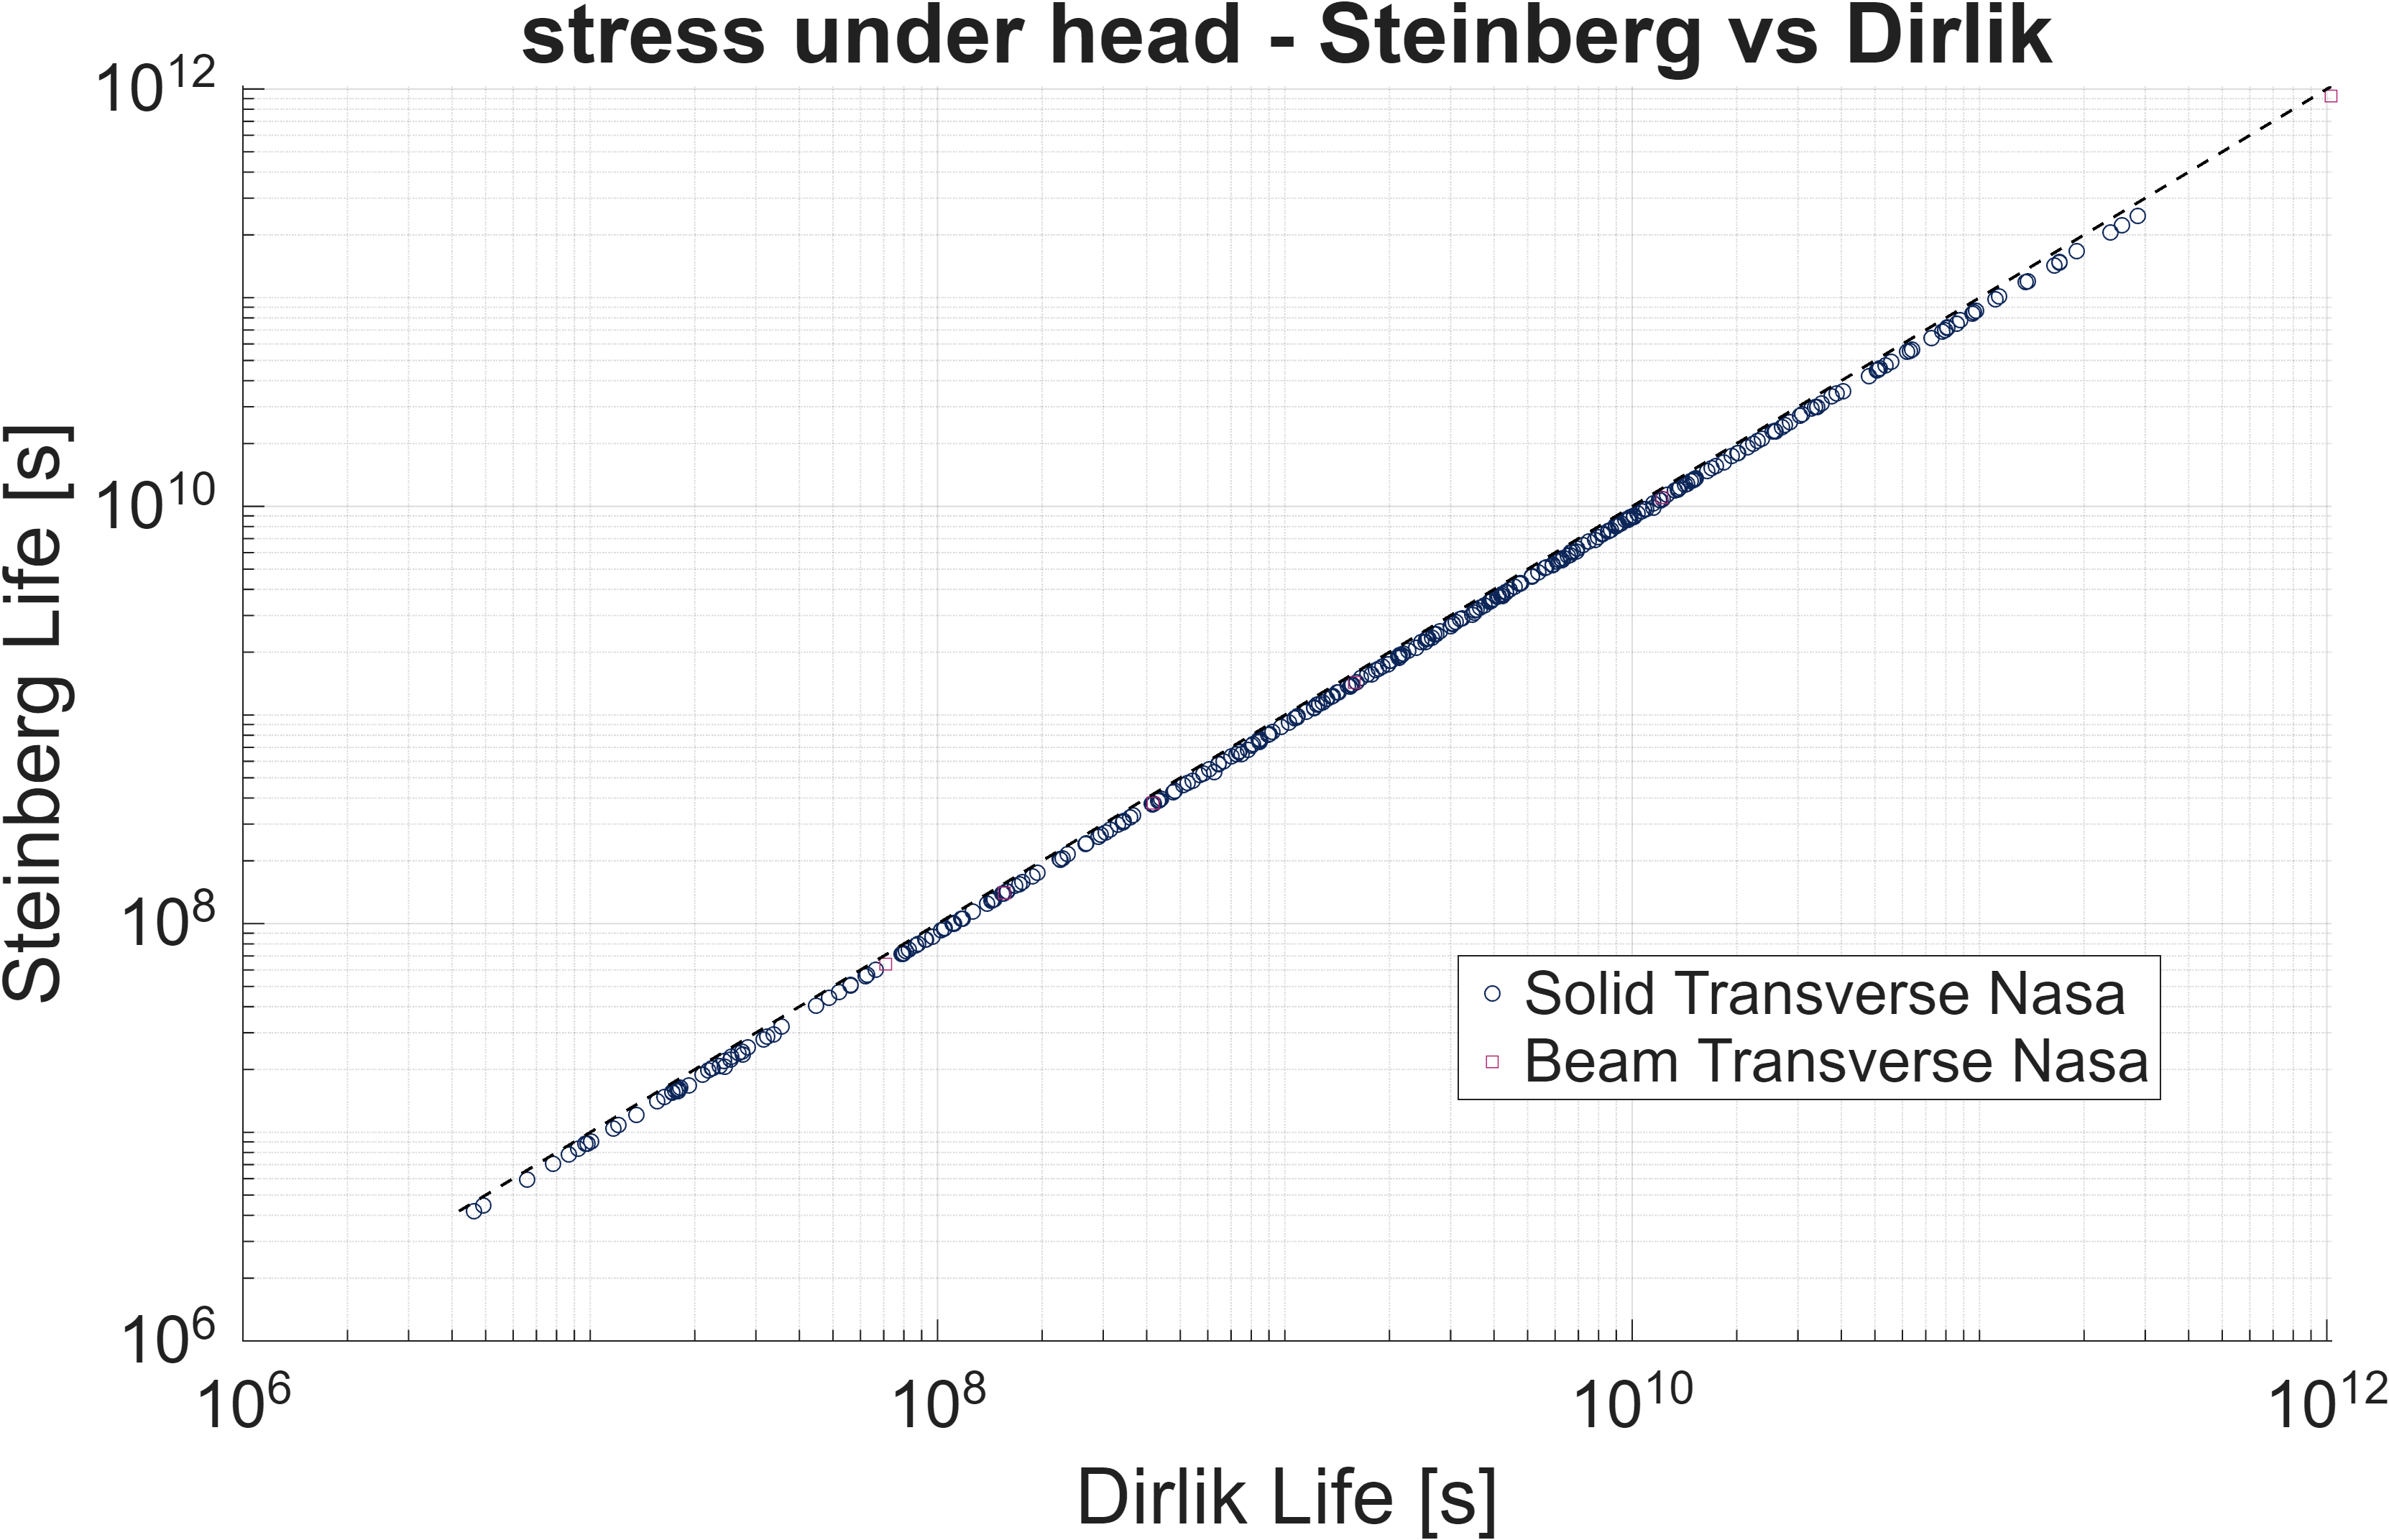
\includegraphics[width=\textwidth]{Transverse Nasa/Transverse Nasa_steinberg_vs_dirlik_NODEWISE stress_under_head.png}
        \caption{Transverse Loading (shear).}
        \label{fig:NASA_shear_steinberg_vs_dirlik_NODEWISE_stress_under_head}
    \end{subfigure}
    \begin{subfigure}[b]{0.45\textwidth}
        \centering
        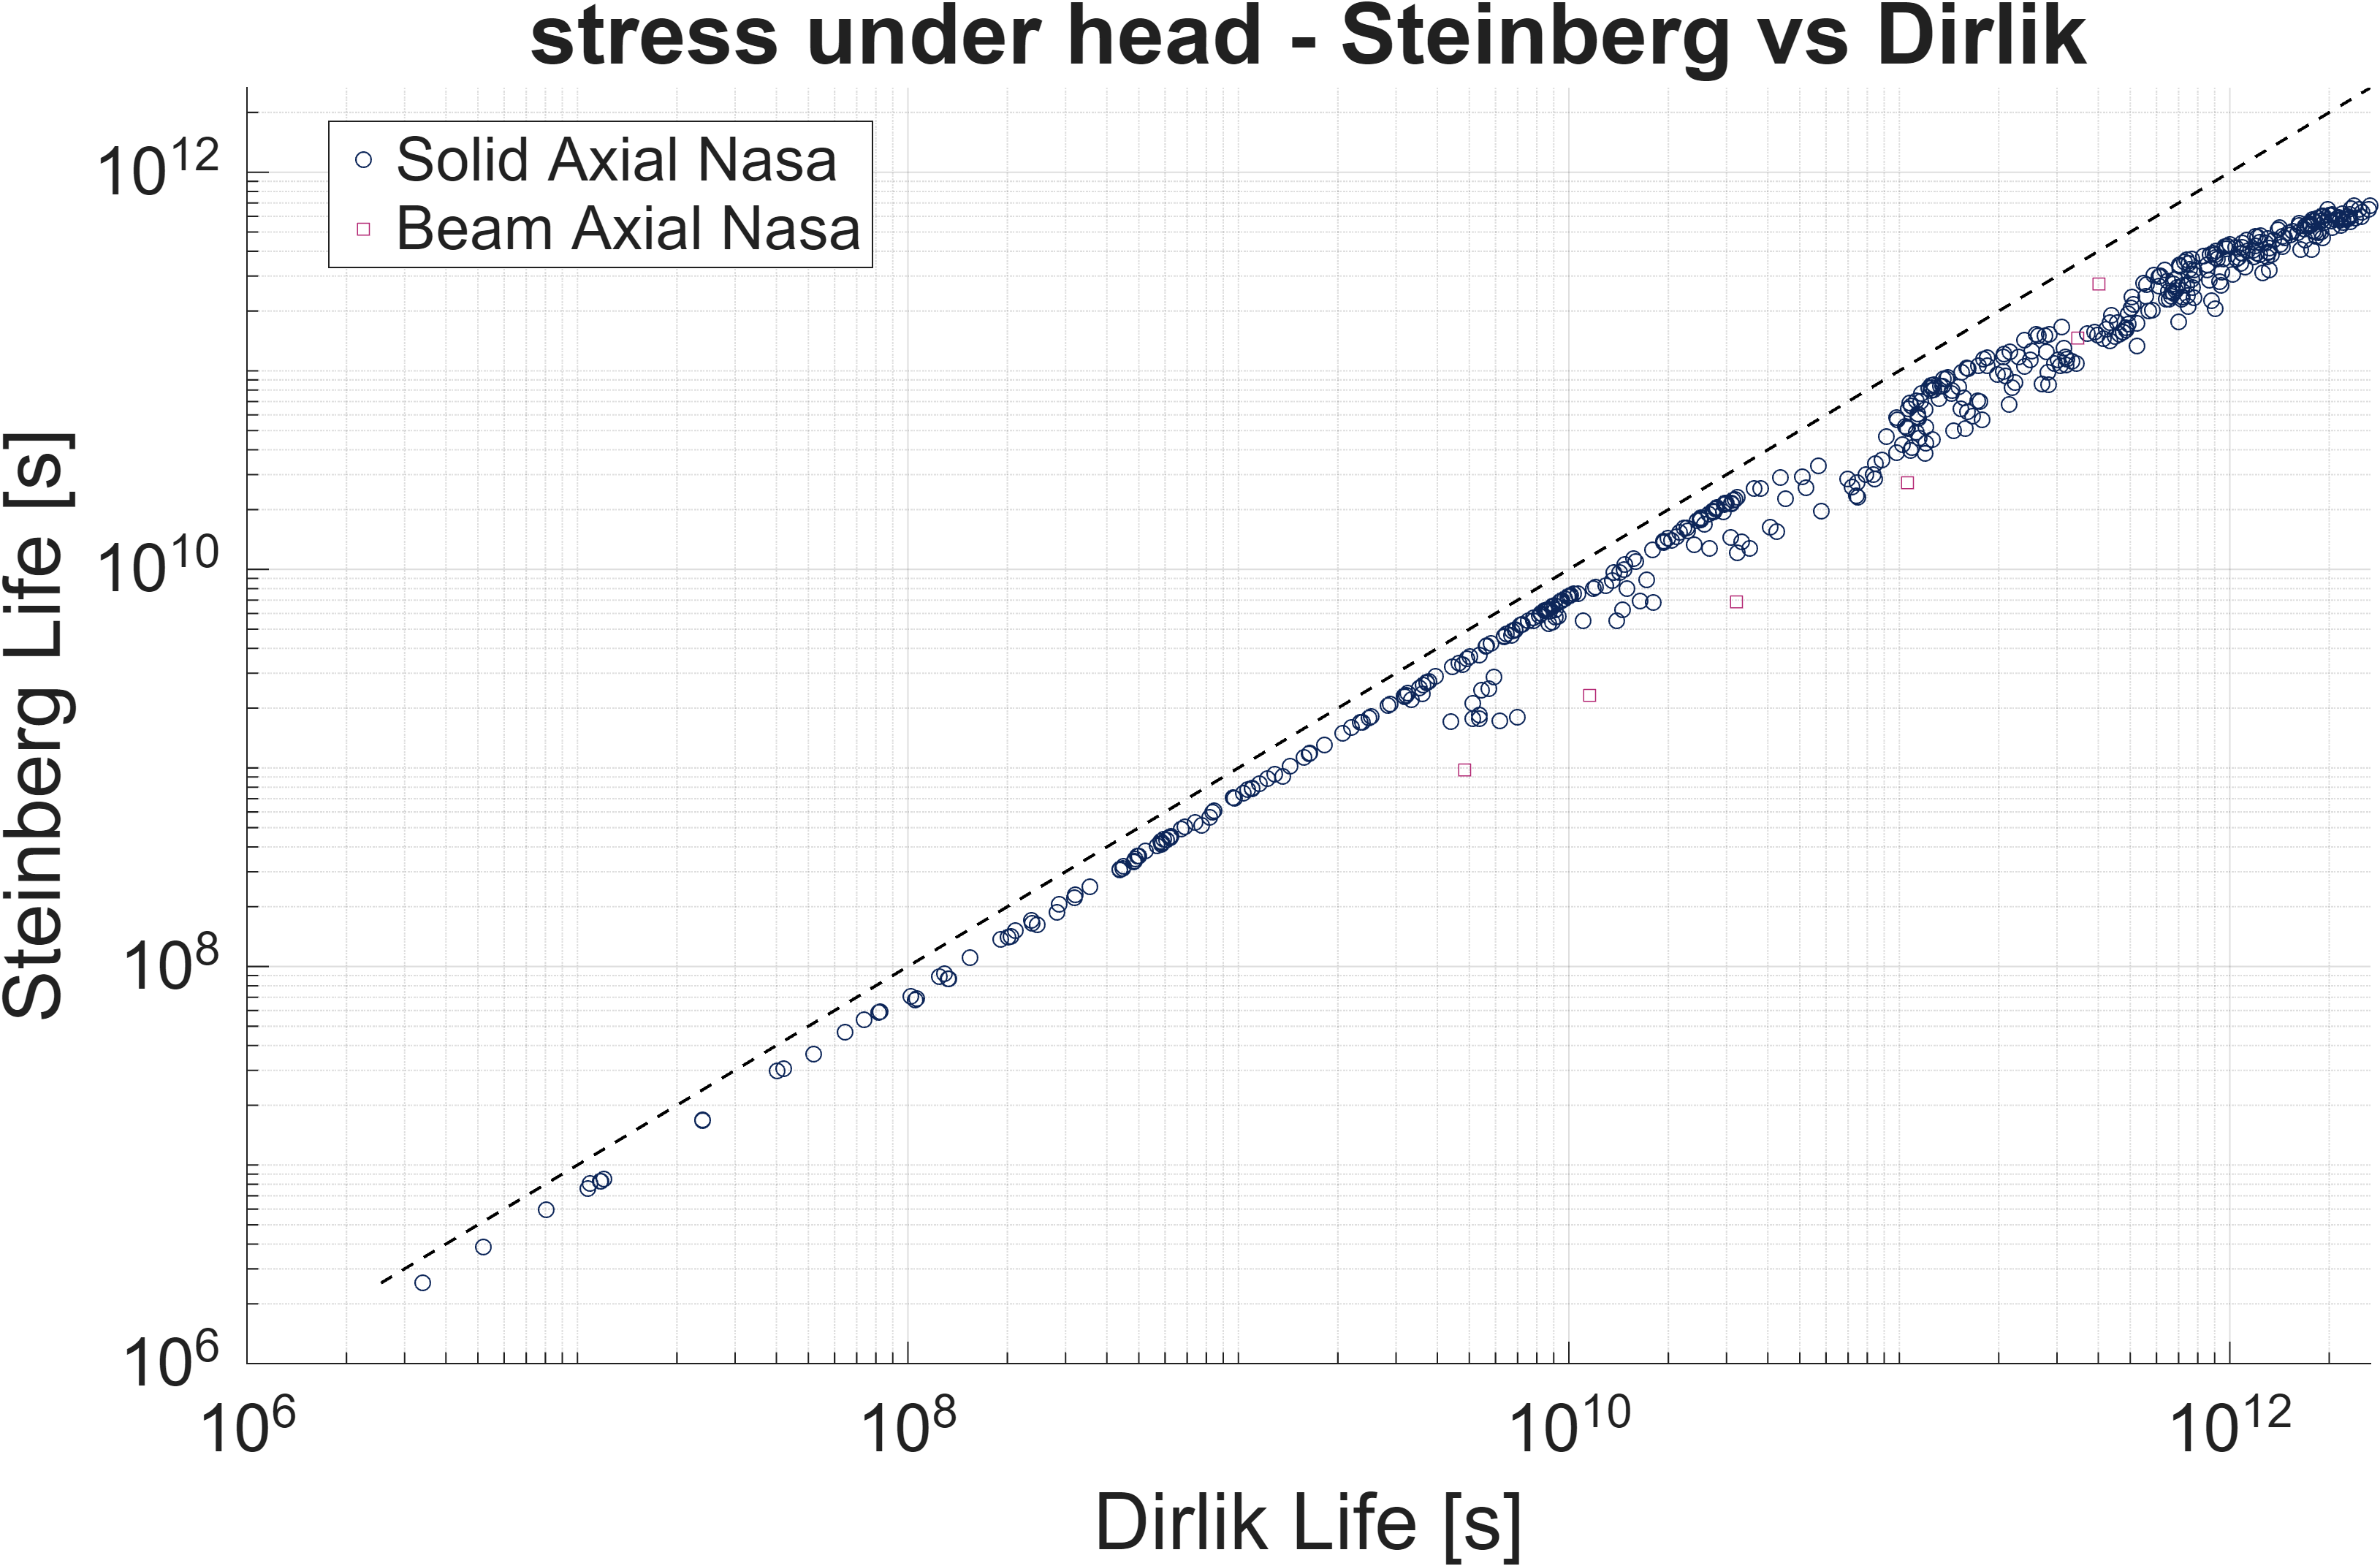
\includegraphics[width=\textwidth]{Axial Nasa/Axial Nasa_steinberg_vs_dirlik_NODEWISE stress_under_head.png}
        \caption{Axial Loading (bending).}
        \label{fig:NASA_bending_steinberg_vs_dirlik_NODEWISE_stress_under_head}
    \end{subfigure}
    
    \caption{Steinberg versus Dirlik fatigue life for the under-head region (solid- and beam representation only). The same trends are visible in the corresponding T43A results, see Appendix \ref{app:T43A_figures}.}
    \label{fig:SteinbergDirlik_underHead}
\end{figure}

\begin{figure}[H]
    \centering
    \begin{subfigure}[b]{0.45\textwidth}
        \centering
        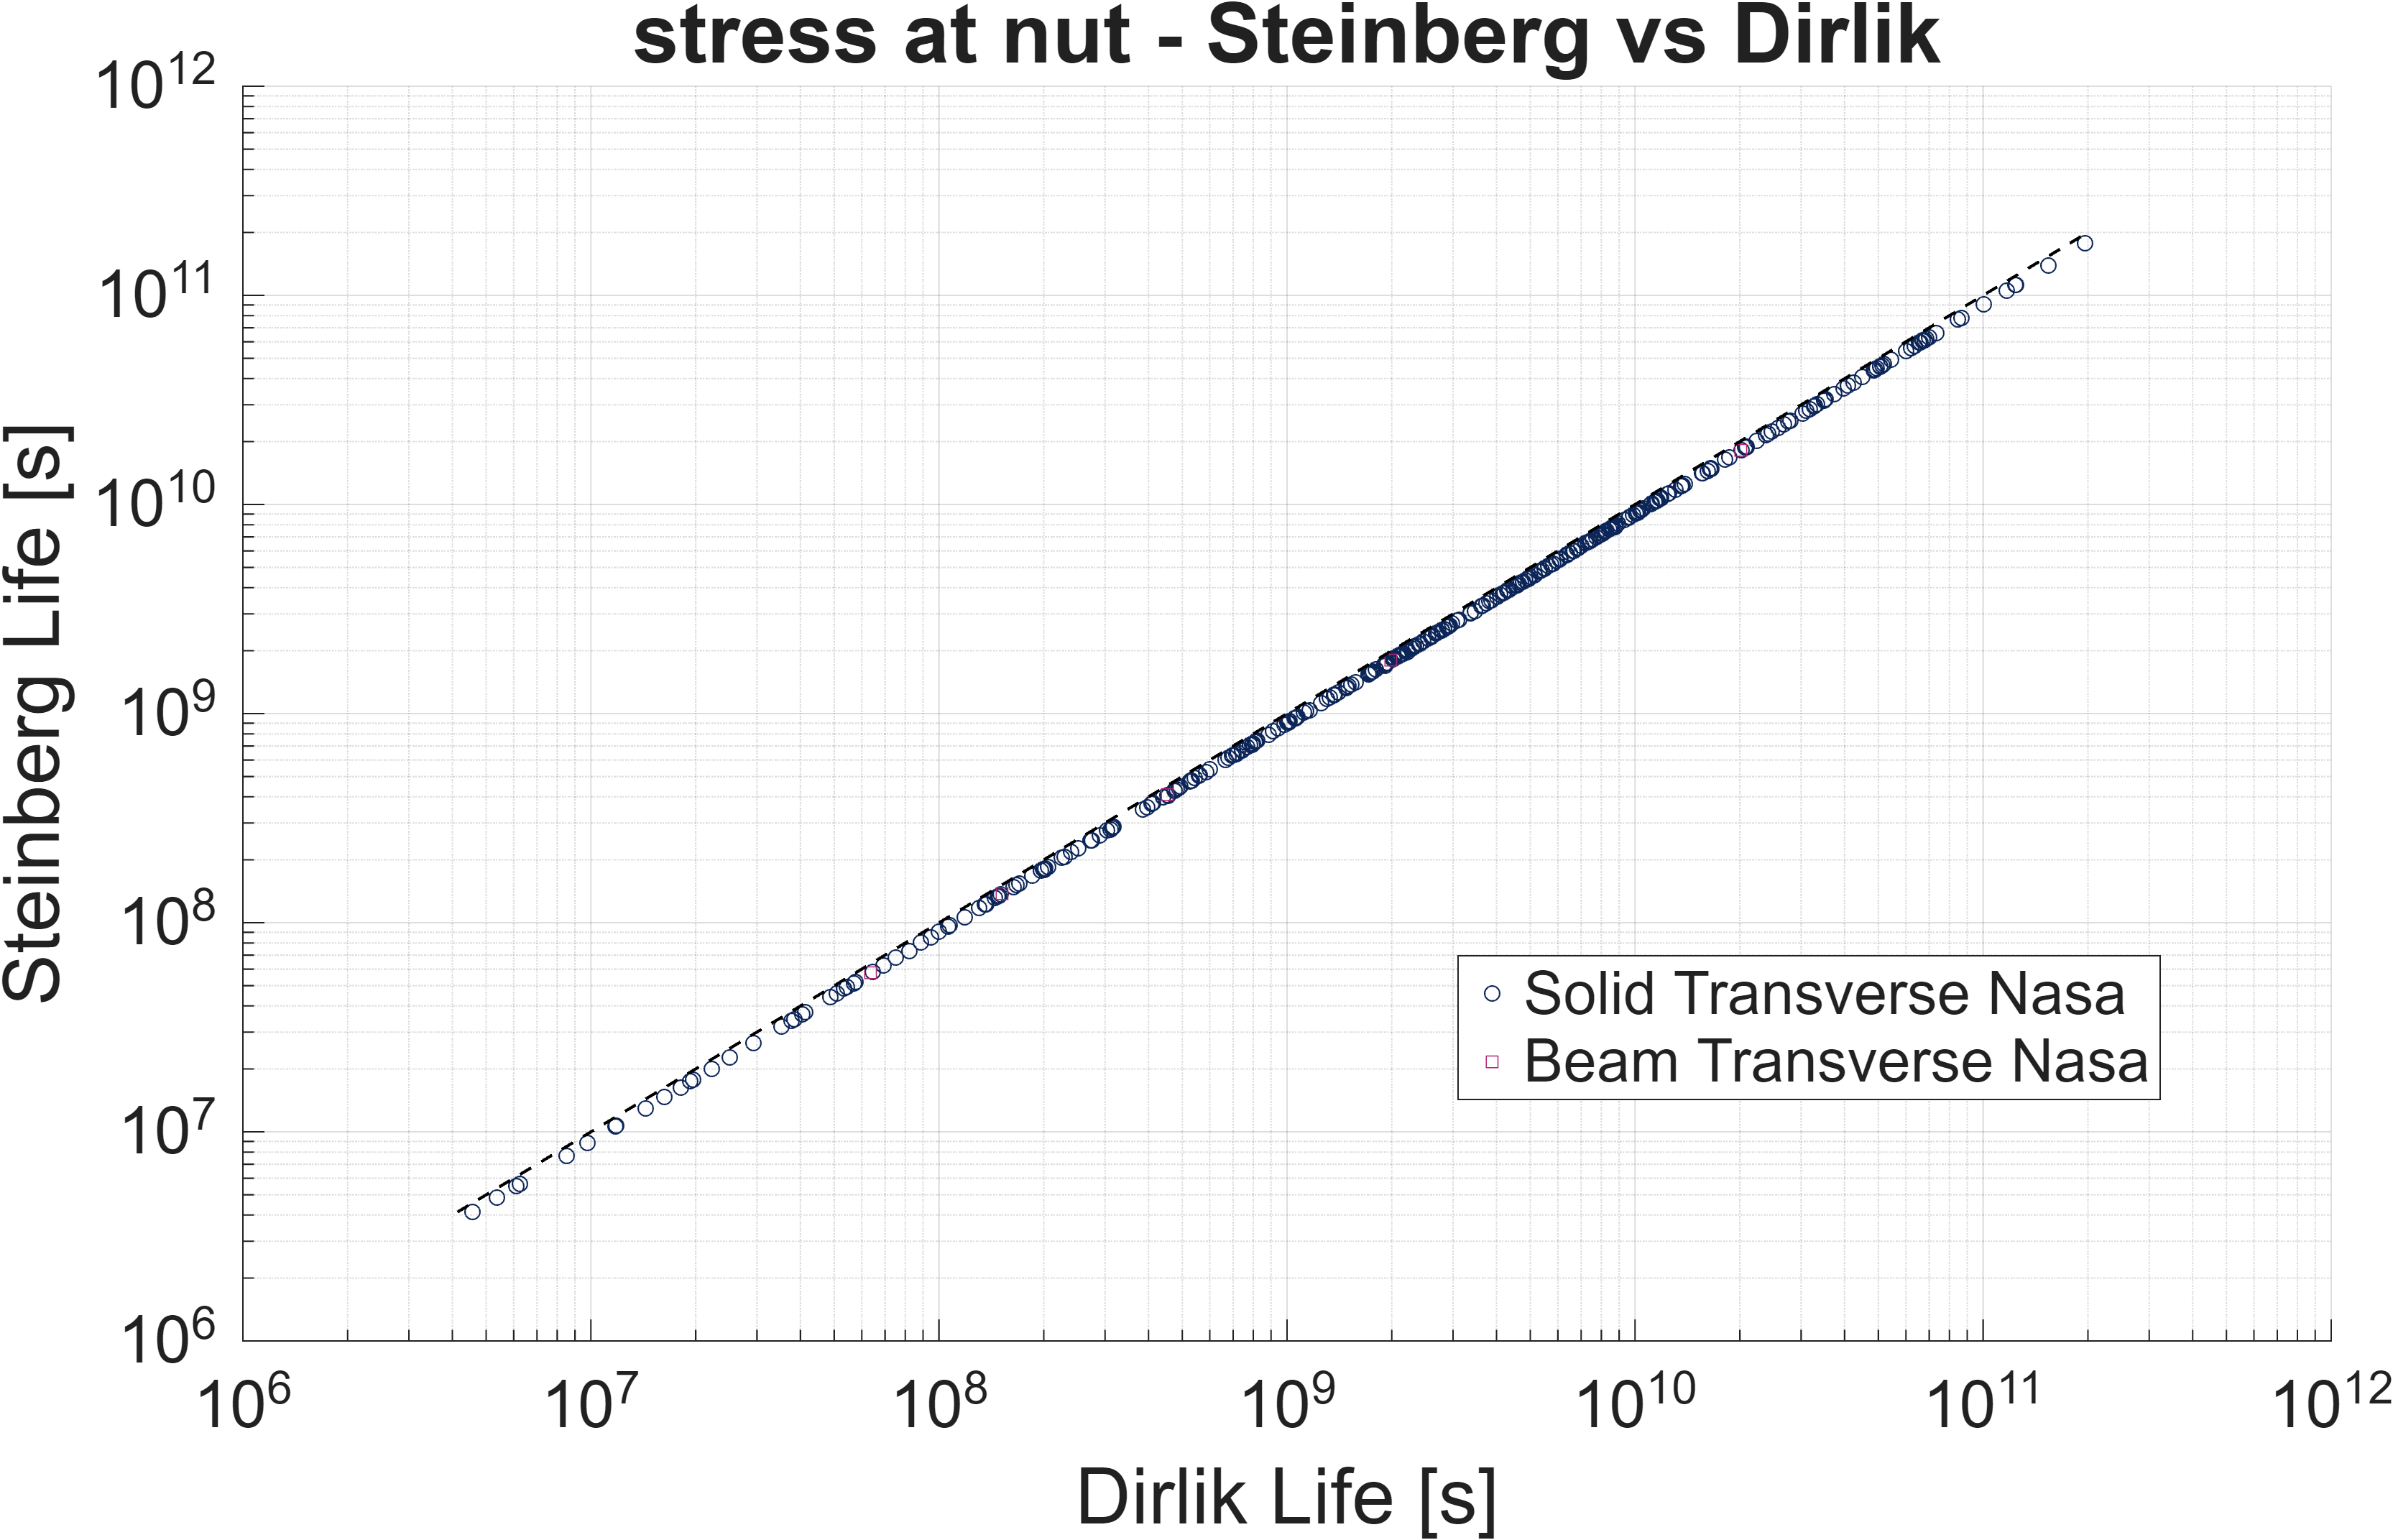
\includegraphics[width=\textwidth]{Transverse Nasa/Transverse Nasa_steinberg_vs_dirlik_NODEWISE stress_at_nut.png}
        \caption{Transverse Loading (shear).}
        \label{fig:NASA_shear_steinberg_vs_dirlik_NODEWISE_stress_at_nut}
    \end{subfigure}
    \begin{subfigure}[b]{0.45\textwidth}
        \centering
        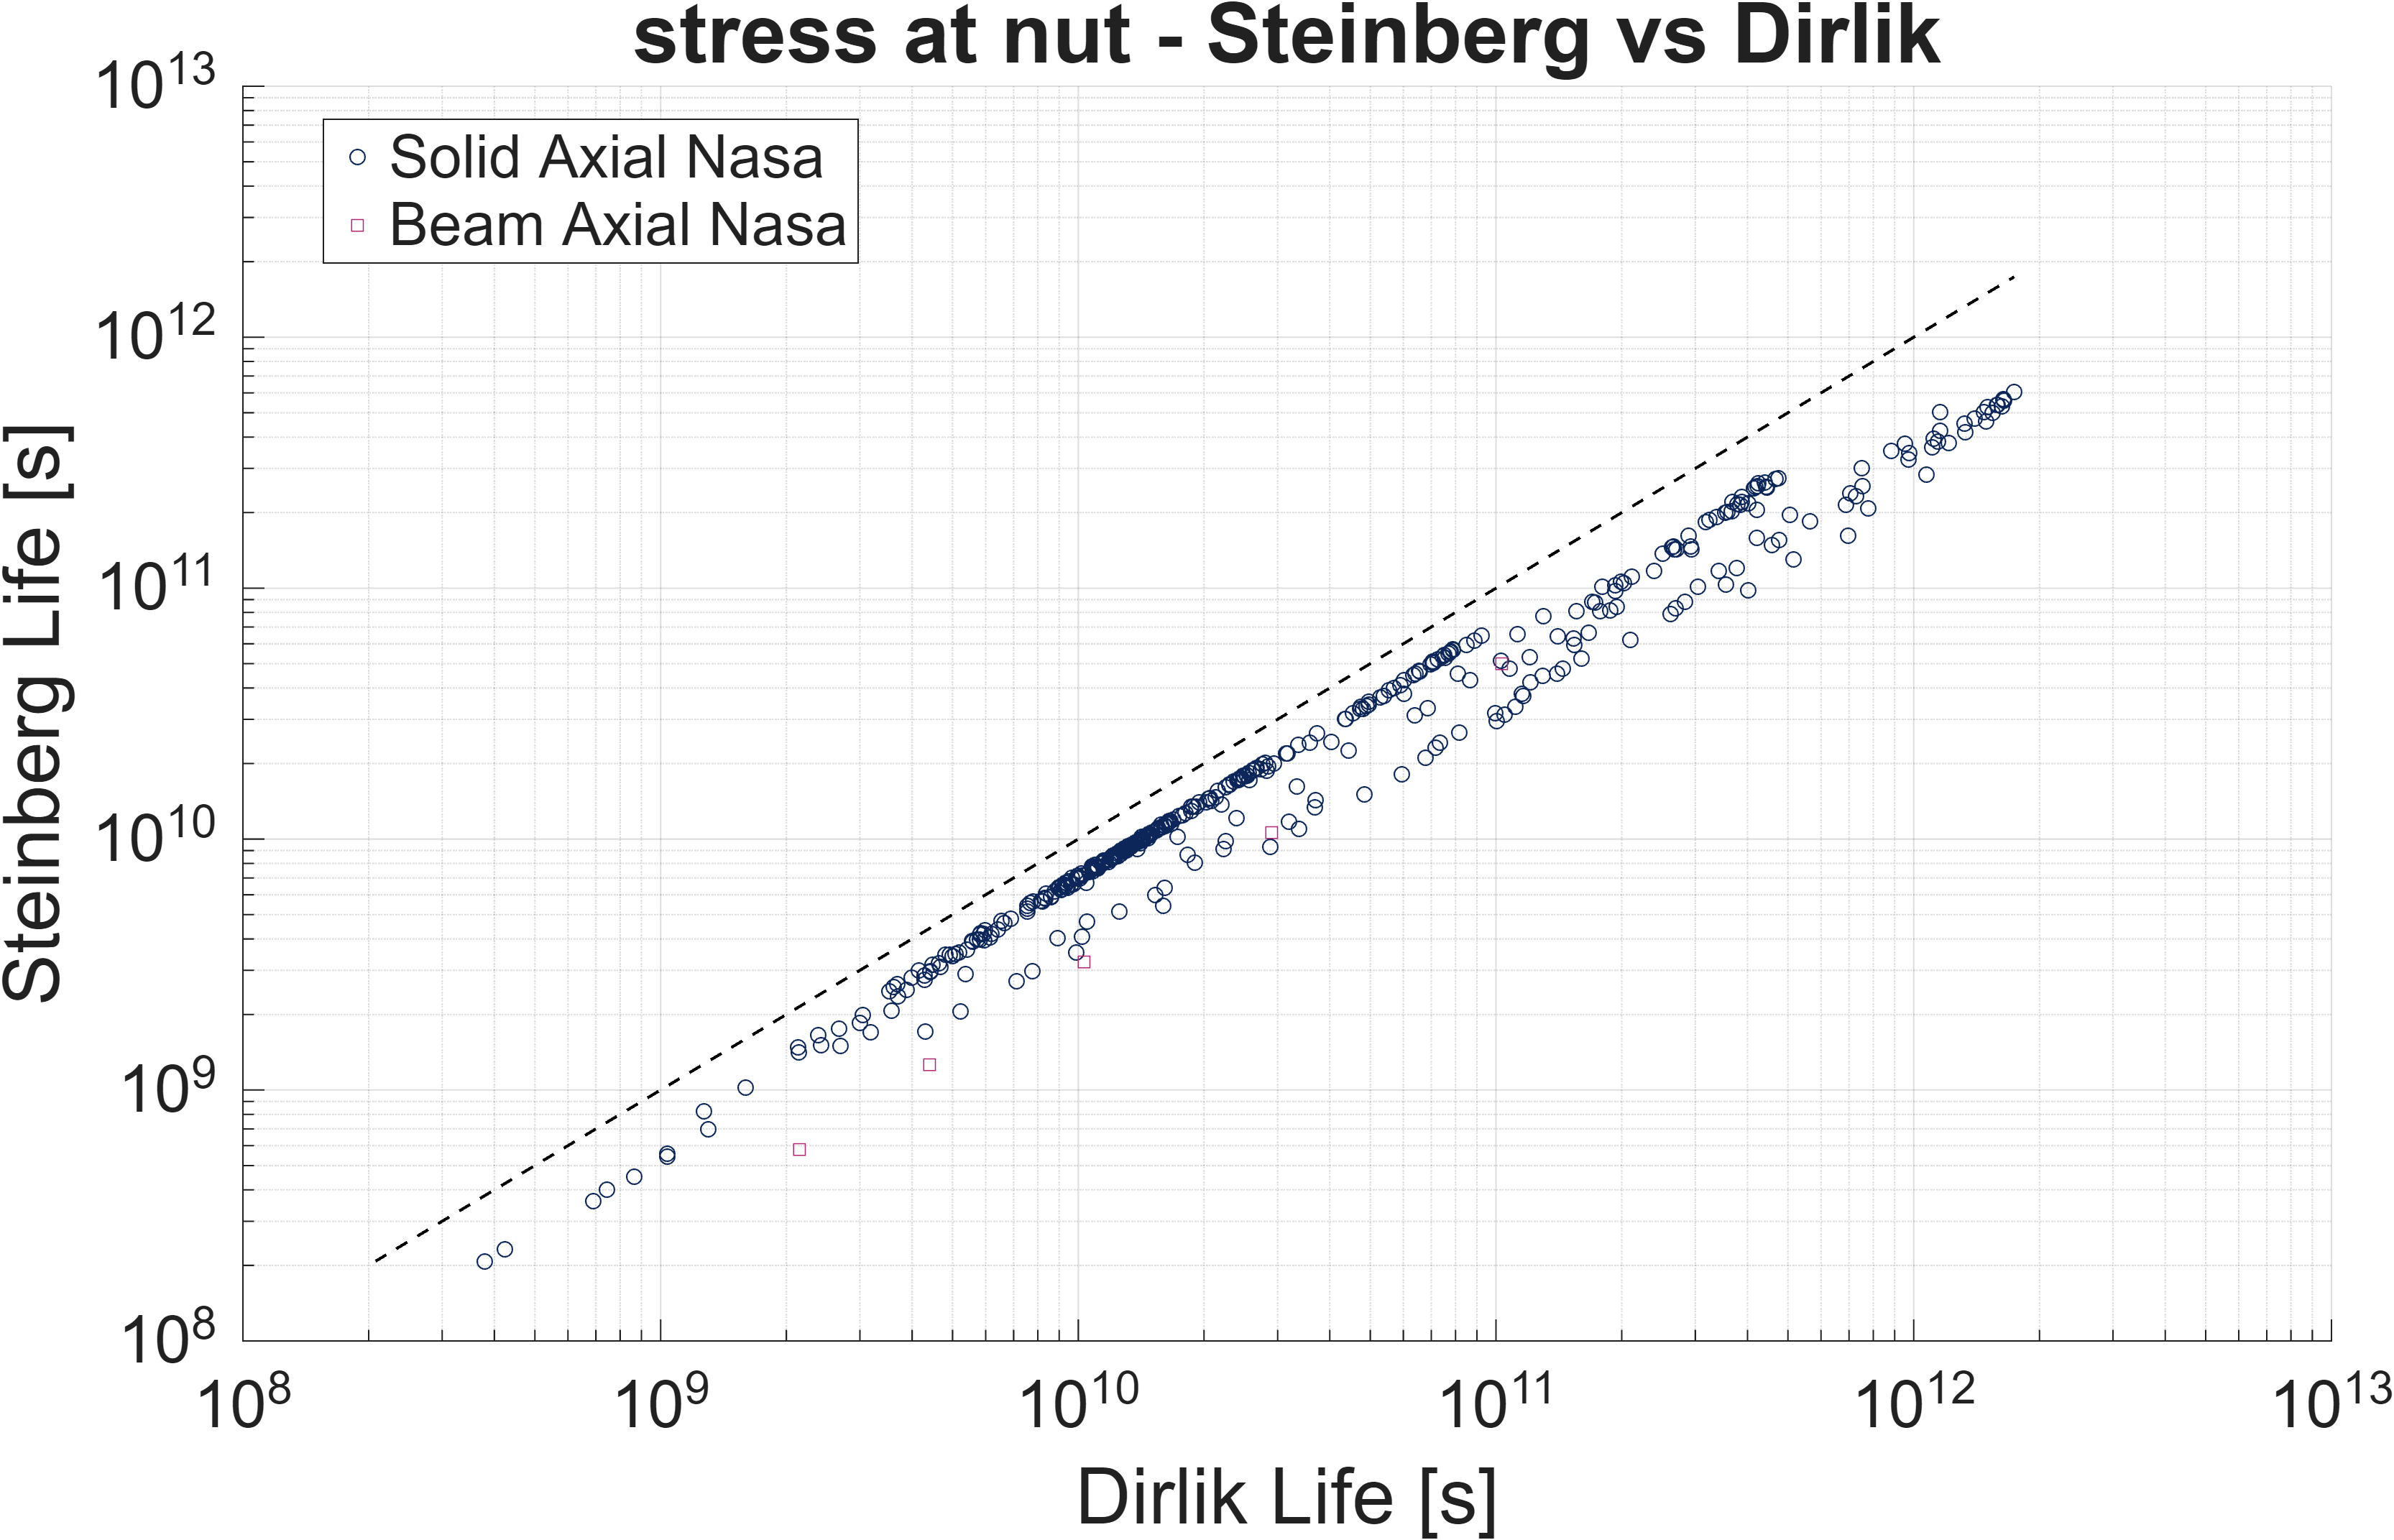
\includegraphics[width=\textwidth]{Axial Nasa/Axial Nasa_steinberg_vs_dirlik_NODEWISE stress_at_nut.png}
        \caption{Axial Loading (bending).}
        \label{fig:NASA_bending_steinberg_vs_dirlik_NODEWISE_stress_at_nut}
    \end{subfigure}
    
    \caption{Steinberg versus Dirlik fatigue life for the at-nut region (solid- and beam representation only). The same trends are visible in the corresponding T43A results, see Appendix \ref{app:T43A_figures}.}
    \label{fig:SteinbergDirlik_atNut}
\end{figure}

The important conclusion is that the relative ranking of the bolt models is not due to the difference between the two fatigue methods. The critical nodes remain critical in both formulations. The beam model remains critical in both formulations and remains the closest approximation to the solid reference in the clamped members region. The Dirlik formulation remains the primary formulation in this thesis because it is better suited to broadband random vibration loading and utilizes the full spectral information contained in the \ac{PSD} \cite{halfpenny_frequency_1999}, \cite{72}, \cite{dirlik_application_1985}.

\newpage
\section{Ranking Index, cost and efficiency results} \label{sec:Tornado}

The Ranking Index (Equation \ref{eq:AccuracyMetric}) combines three errors with weights: minimum Dirlik fatigue life (weight 0.50), the relative error of the maximum \ac{RMS} von Mises stress (weight 0.30), and the relative error of the 95th-percentile \ac{RMS} von Mises stress (weight 0.20). These weights are not the only defensible choice. To test if the model ranking is a robust feature of data instead of just the weighting model, the Ranking Index is recomputed under four alternative weight scenarios, comparing different engineering priorities, as seen in Table \ref{tab:RI_weight_compare}:

\begin{table}[H]
    \centering
    \caption{Weight scenarios for sensitivity checking}
    \label{tab:RI_weight_compare}
    \begin{tabular}{lccc}
        \hline
        Scenario & $w_{life}$ & $w_{max-RMS}$ & $w_{95-RMS}$ \\
        \hline
        Fatigue-first & 0.50 & 0.30 & 0.20 \\
        RMS-first & 0.20 & 0.50 & 0.30 \\
        Equal weights & 1/3 & 1/3 & 1/3 \\
        Life-only & 1.00 & 0.00 & 0.00 \\
        \hline
    \end{tabular}
\end{table}

Figure \ref{fig:tornado} shows a tornado plot for the clamped members region under the NASA-STD-7001B Workmanship excitation. Each bar shows the Ranking Index span for a given bolt model across the four weight scenarios. The bar end-points are the minimum and maximum Ranking Index, and the bar length is therefore a measure of the sensitivity to the weight choice. A short span indicates the model score is insensitive to the selected weights, whereas a long span indicates the score is strongly dependent on the engineering priority.

\begin{figure}[H]
    \centering
    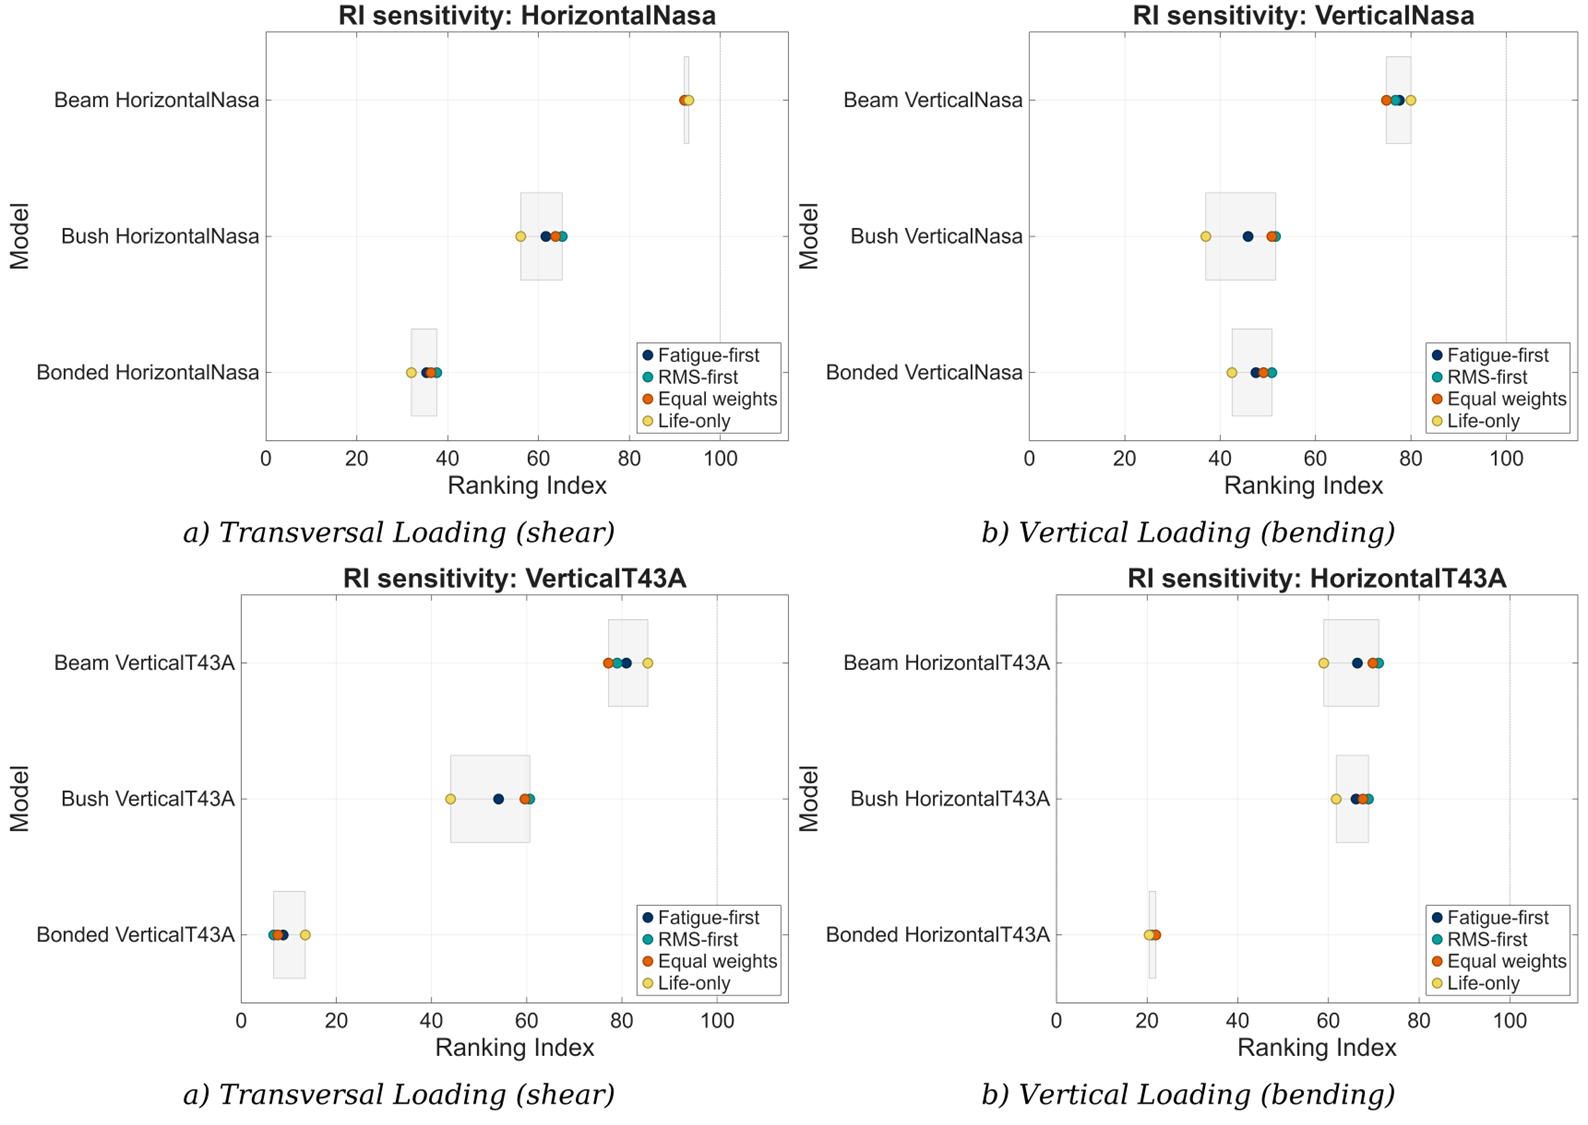
\includegraphics[width=0.96\linewidth]{Figures/Tornado.png}
    \caption{Tornado plot of the sensitivity for weighting in the Ranking Index.}
    \label{fig:tornado}
\end{figure}

The main finding is that the model ranking is unchanged in two of the four load cases: Transverse NASA and Axial T43A. All weight scenarios gave the strict order beam - CBUSH - bonded. In the Axial NASA and Transverse T43A, the beam still ranks first under fatigue-first, RMS-first, and equal-weight scenarios. Only the CBUSH-bonded ordering swaps in Axial NASA, and the CBUSH narrowly overtakes the beam in the life-only scenario for Transverse T43A. Looking at each model and load case isolated, 8 of 12 rank positions are preserved across all four weight scenarios.

The CBUSH has the largest sensitivity span, reaching 16.6 for axial T43A and 14.6 for axial NASA, because its life error is relatively large while its \ac{RMS} errors are lower. The CBUSH is more effective when RMS-related terms are prioritized, but less effective (with a lower Ranking Index) when fatigue-life dominates. This causes the bonded and CBUSH models to exchange second and third (last) rank in the axial NASA case, depending on the weight scenario.

The ranking is fully consistent for the transverse NASA and axial T43A cases: 1) beam, 2) CBUSH, 3) bonded. The bonded model scores poorly in the axial T43A with $RI \approx 6.8 - 13.4$, reflecting the large stress over-prediction that is seen in Figure \ref{fig:Stress_PSD_Members_Comparison_T43A}. Overall, the bonded shows sensitivity spans of 1.5-8.3 but consistently low absolute scores.

For transverse T43A, beam and CBUSH have almost the same Ranking Index (RI 66.4 VS 66.1). This difference is too small to support a strong preference and is the only robustness instability. In the life-only scenario, CBUSH ranks first because the beam's life error is higher in this specific load case.

Overall, the tornado plots show that the Ranking Index is a defensible model-selection metric for the clamped-member region. The beam model is consistently the preferred simplified representation of the bolt for vibration-fatigue assessment, regardless of whether fatigue life or \ac{RMS} stress is prioritized in the load cases presented in this thesis.

\subsection{Ranking Index for the different cases}
The left plots in Figure \ref{fig:AccuracyScore_per_region} and \ref{fig:AccuracyMap_per_region} show the Ranking Index for transverse loading. In the clamped-members region, the beam model obtains the highest score among the simplified alternatives at 92.8. The CBUSH model reaches 61.6, and the bonded model scores 35.4. This confirms quantitatively what was already evident in the \ac{PSD} and fatigue-life comparisons: the beam model is the most accurate simplified alternative for the stress response of clamped members for the present benchmark and load case.

\begin{figure}[H]
    \centering
    \begin{subfigure}[b]{0.45\textwidth}
        \centering
        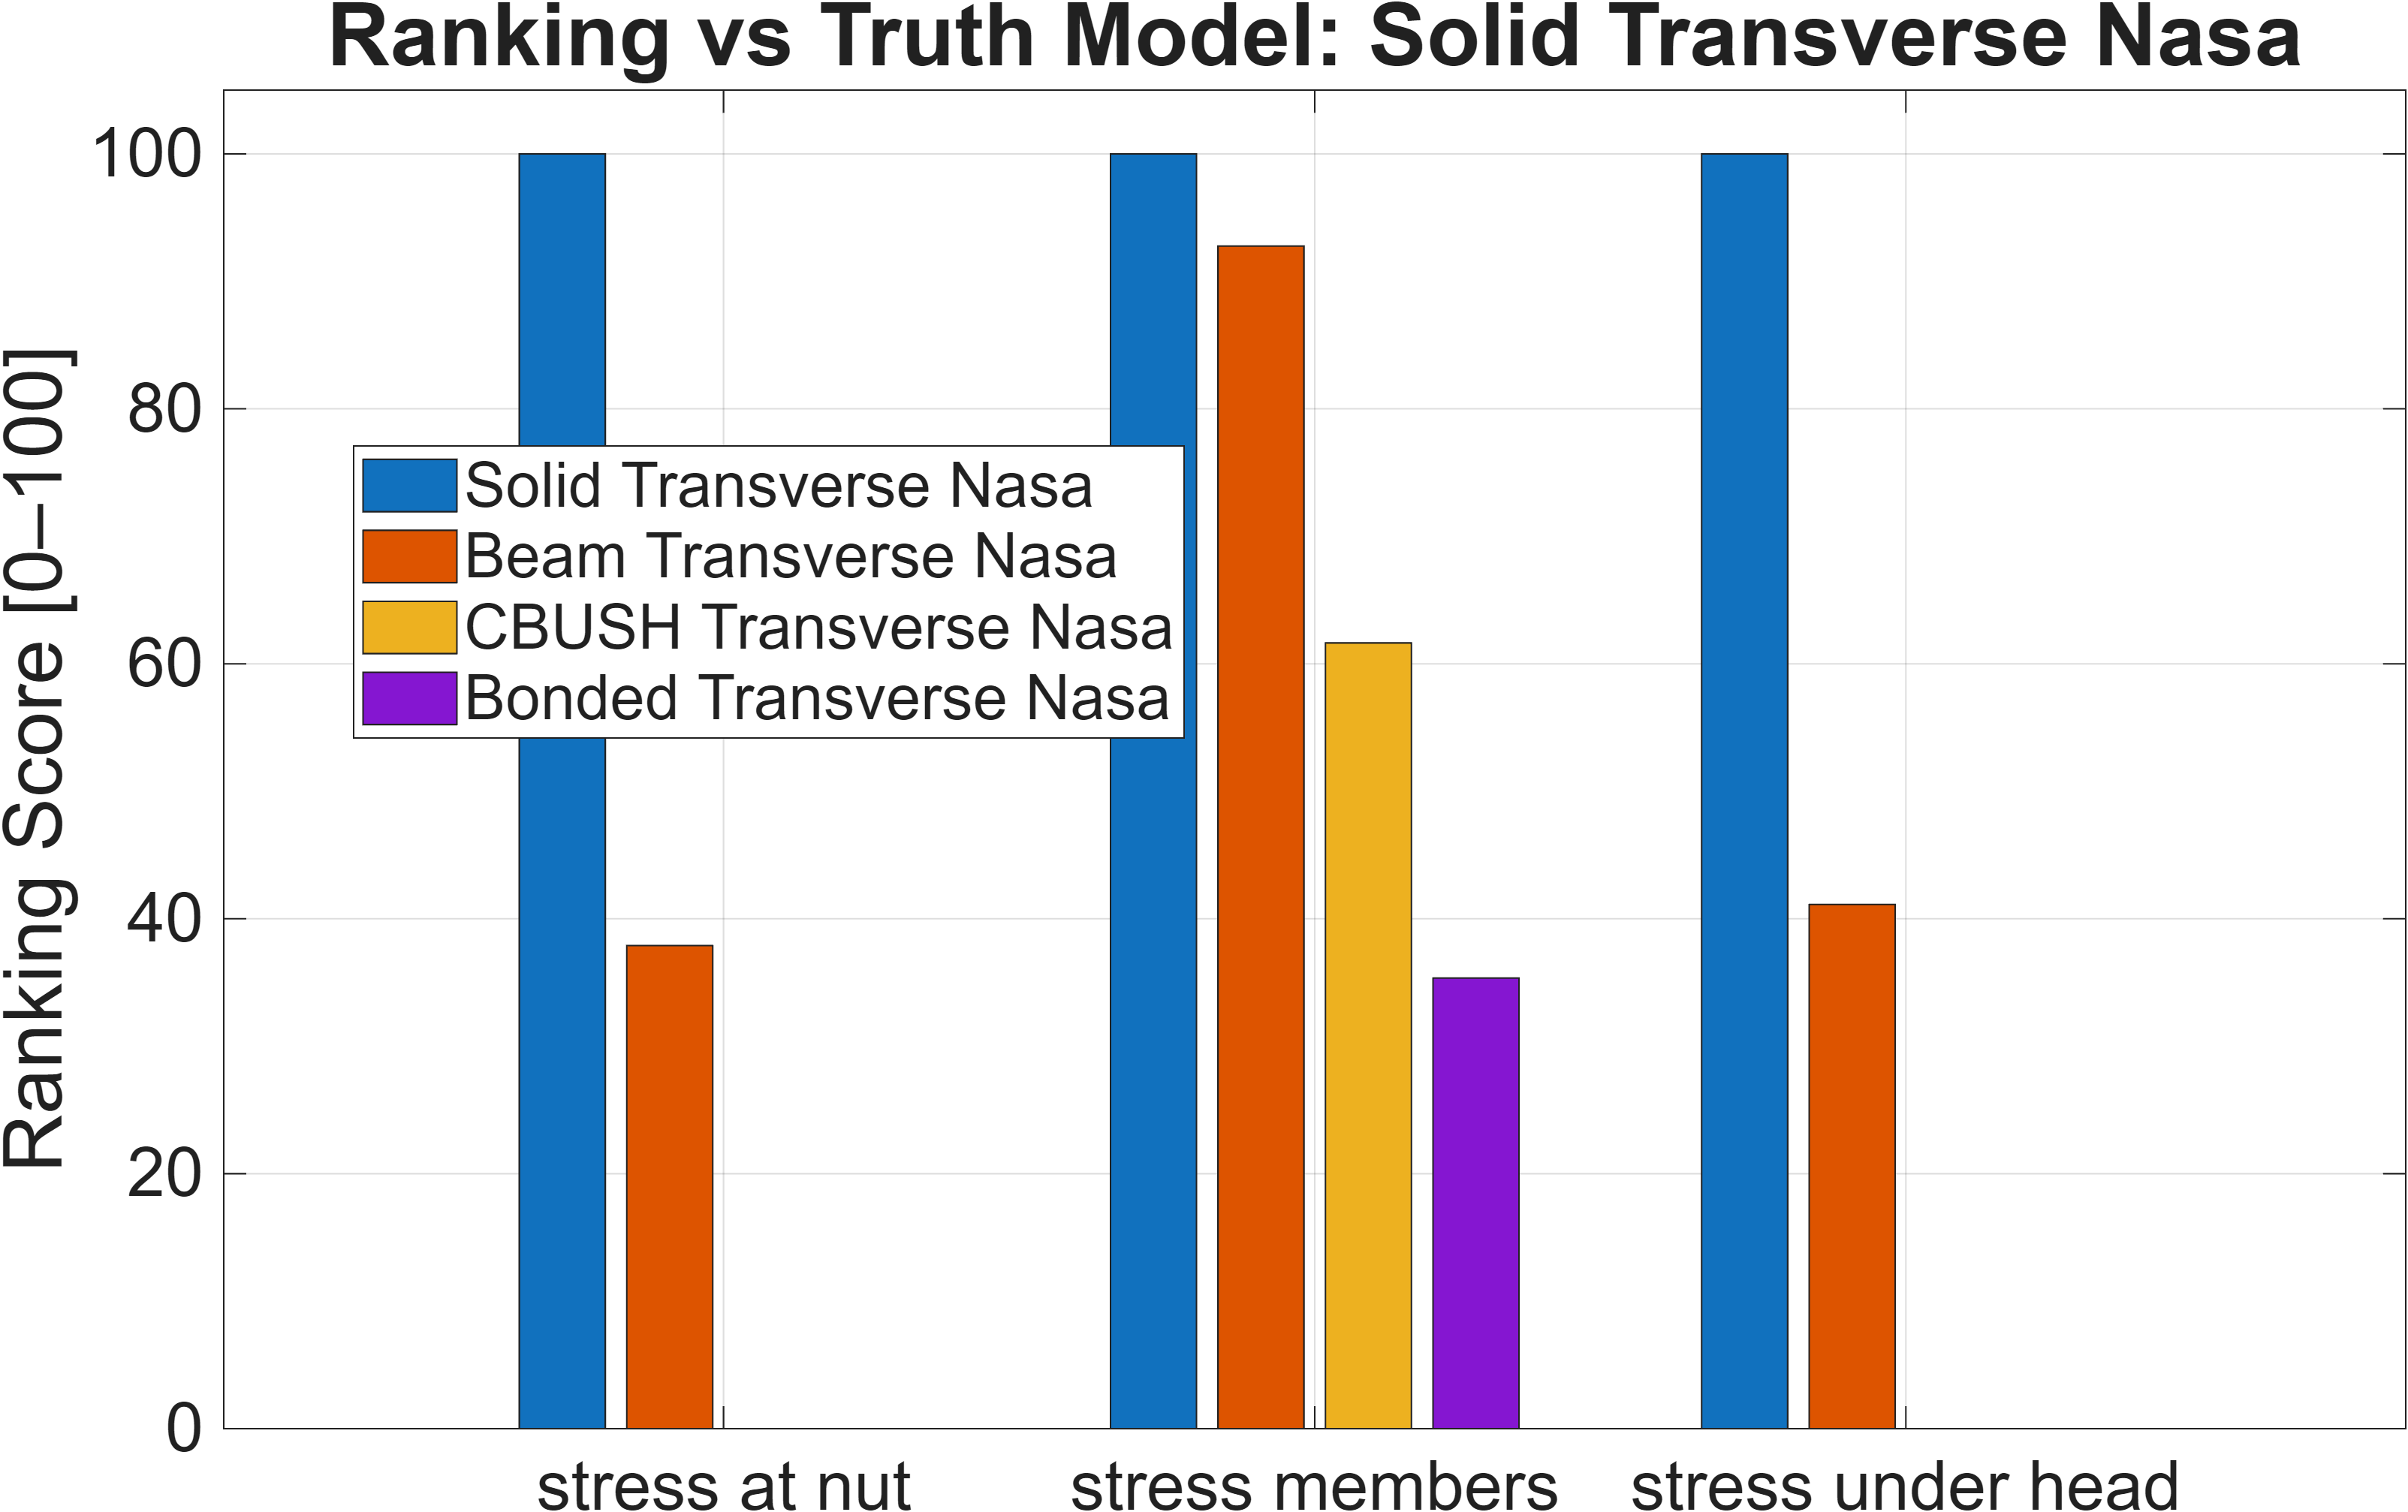
\includegraphics[width=\textwidth]{Transverse Nasa/Transverse Nasa_ranking_score_by_region_and_model NODEWISE.png}
        \caption{Transverse Loading (shear).}
        \label{fig:NASA_shear_ranking_score_by_region_and_model_NODEWISE}
    \end{subfigure}
    \begin{subfigure}[b]{0.45\textwidth}
        \centering
        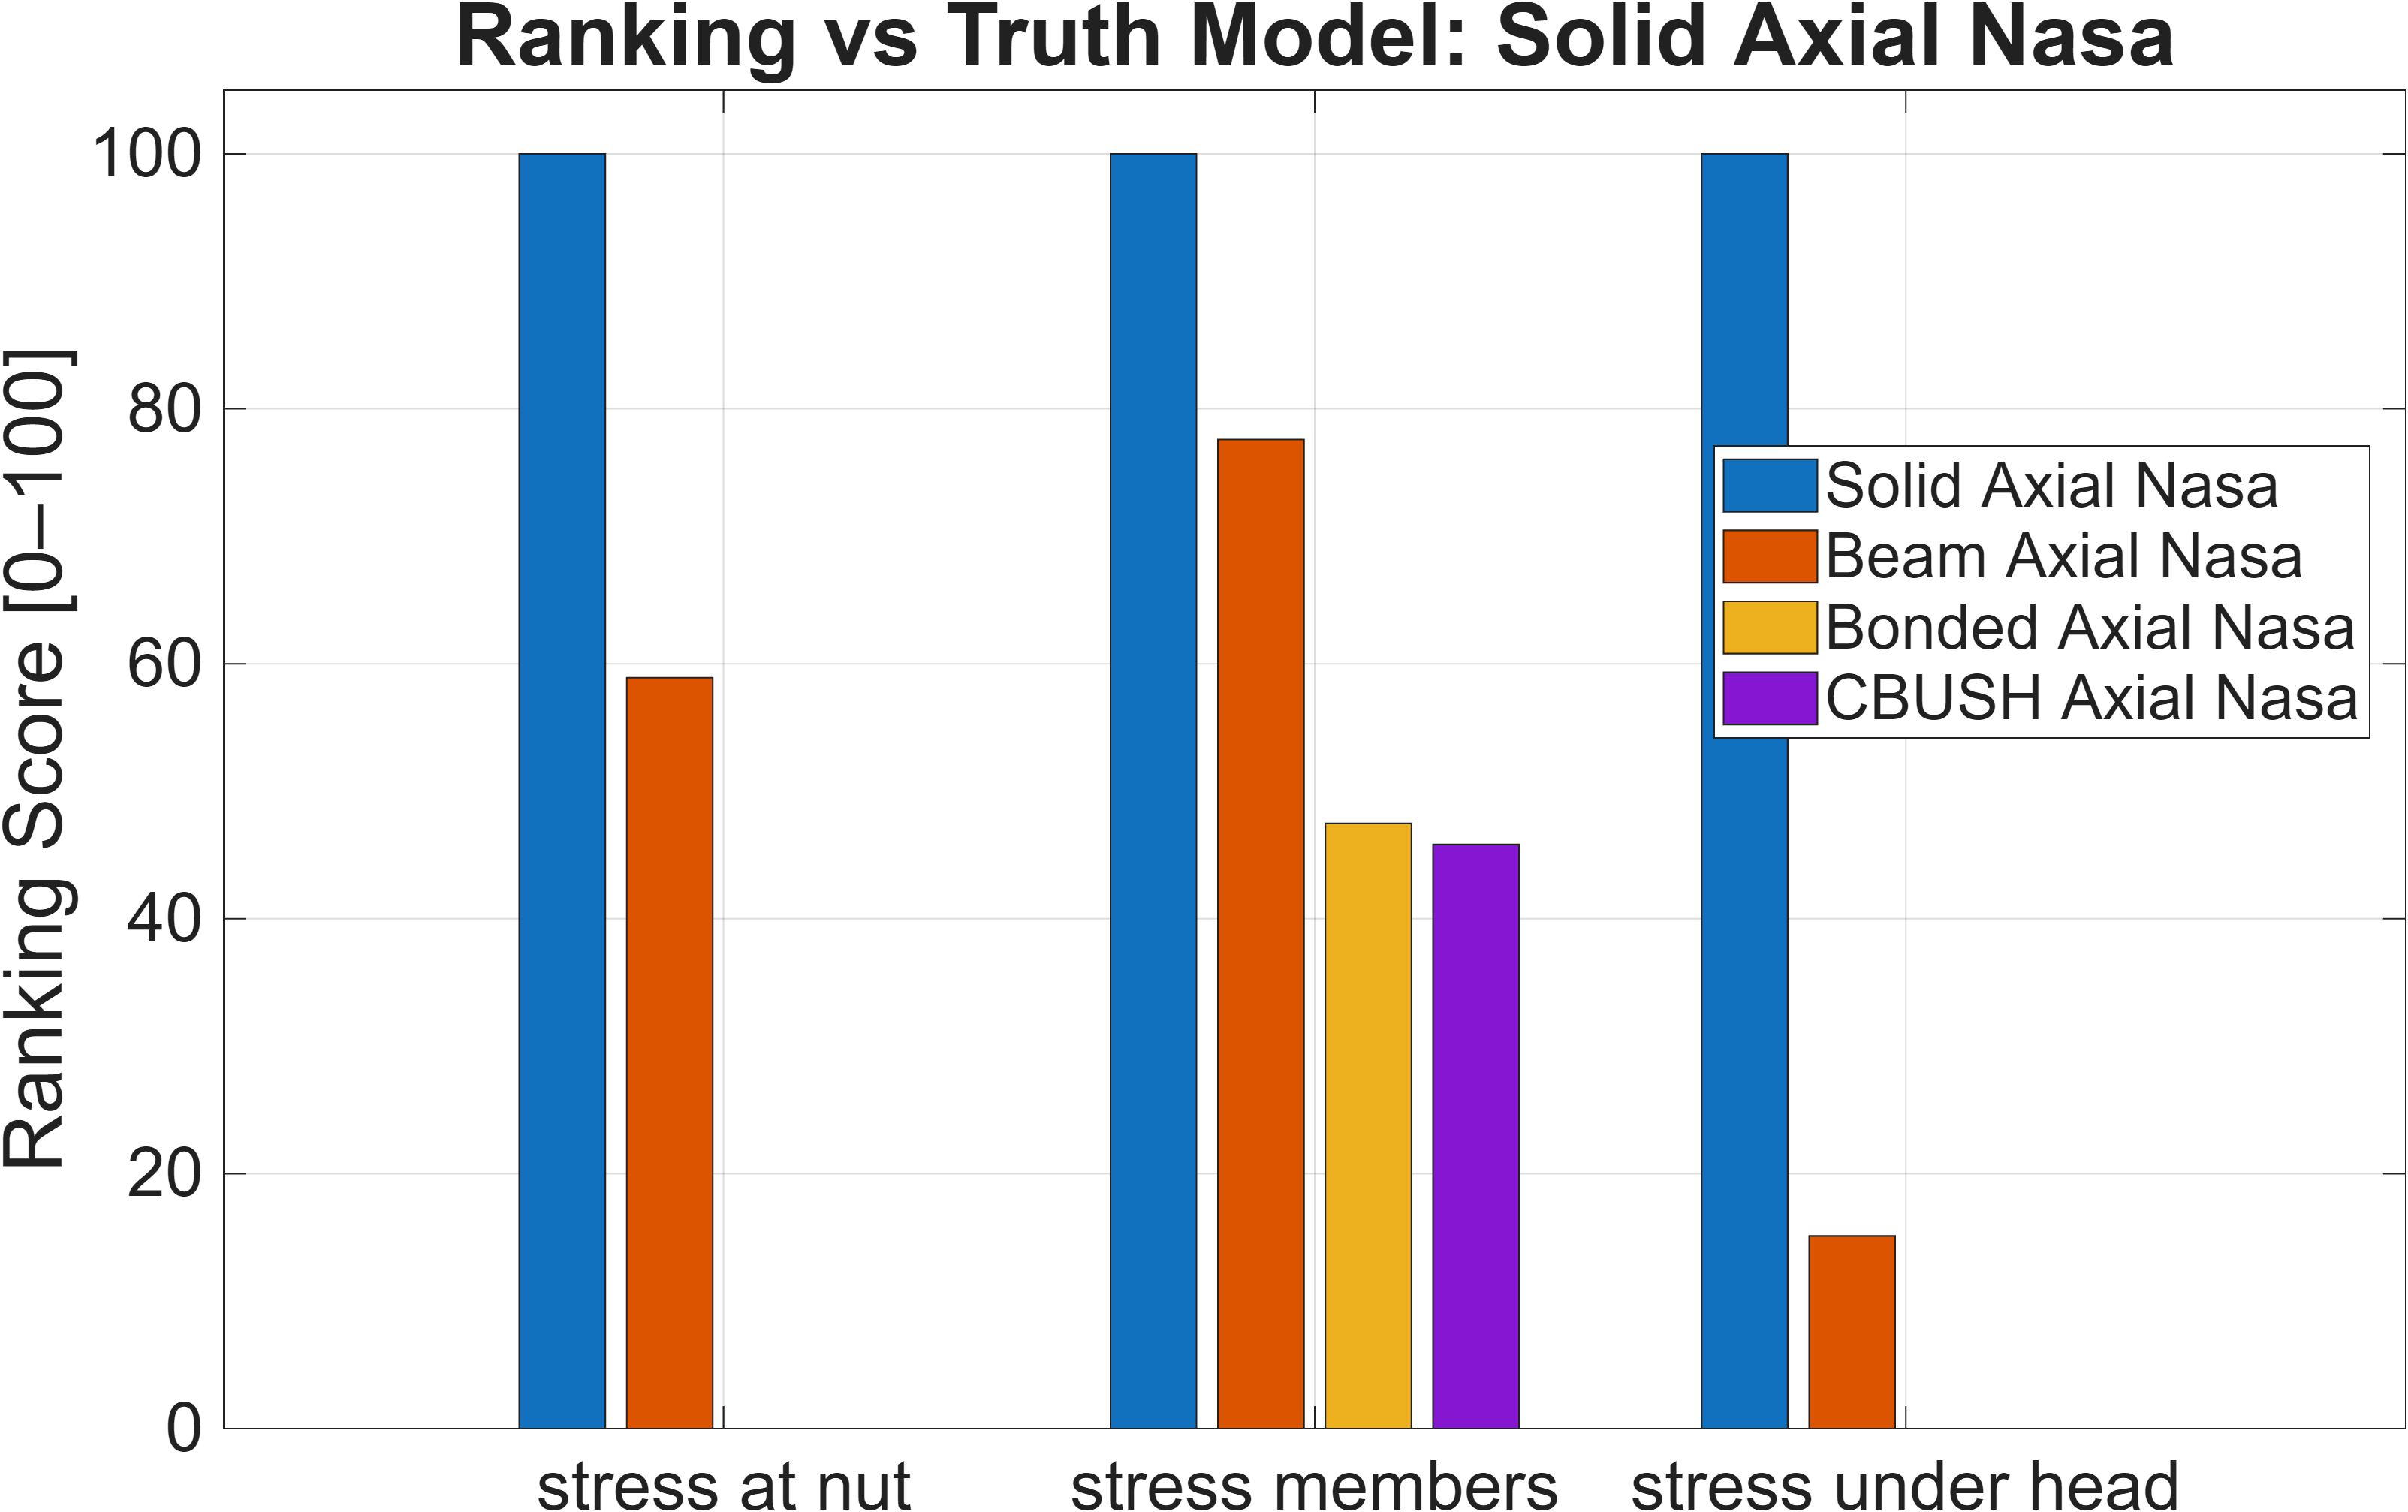
\includegraphics[width=\textwidth]{Axial Nasa/Axial Nasa_ranking_score_by_region_and_model NODEWISE.png}
        \caption{Axial Loading (bending).}
        \label{fig:NASA_bending_ranking_score_by_region_and_model_NODEWISE}
    \end{subfigure}
    
    \caption{Ranking Index per region and test model, relative to the Solid model. The same trends are visible in the corresponding T43A results, see Appendix \ref{app:T43A_figures}.}
    \label{fig:AccuracyScore_per_region}
\end{figure}

\begin{figure}[H]
    \centering
    \begin{subfigure}[b]{0.45\textwidth}
        \centering
        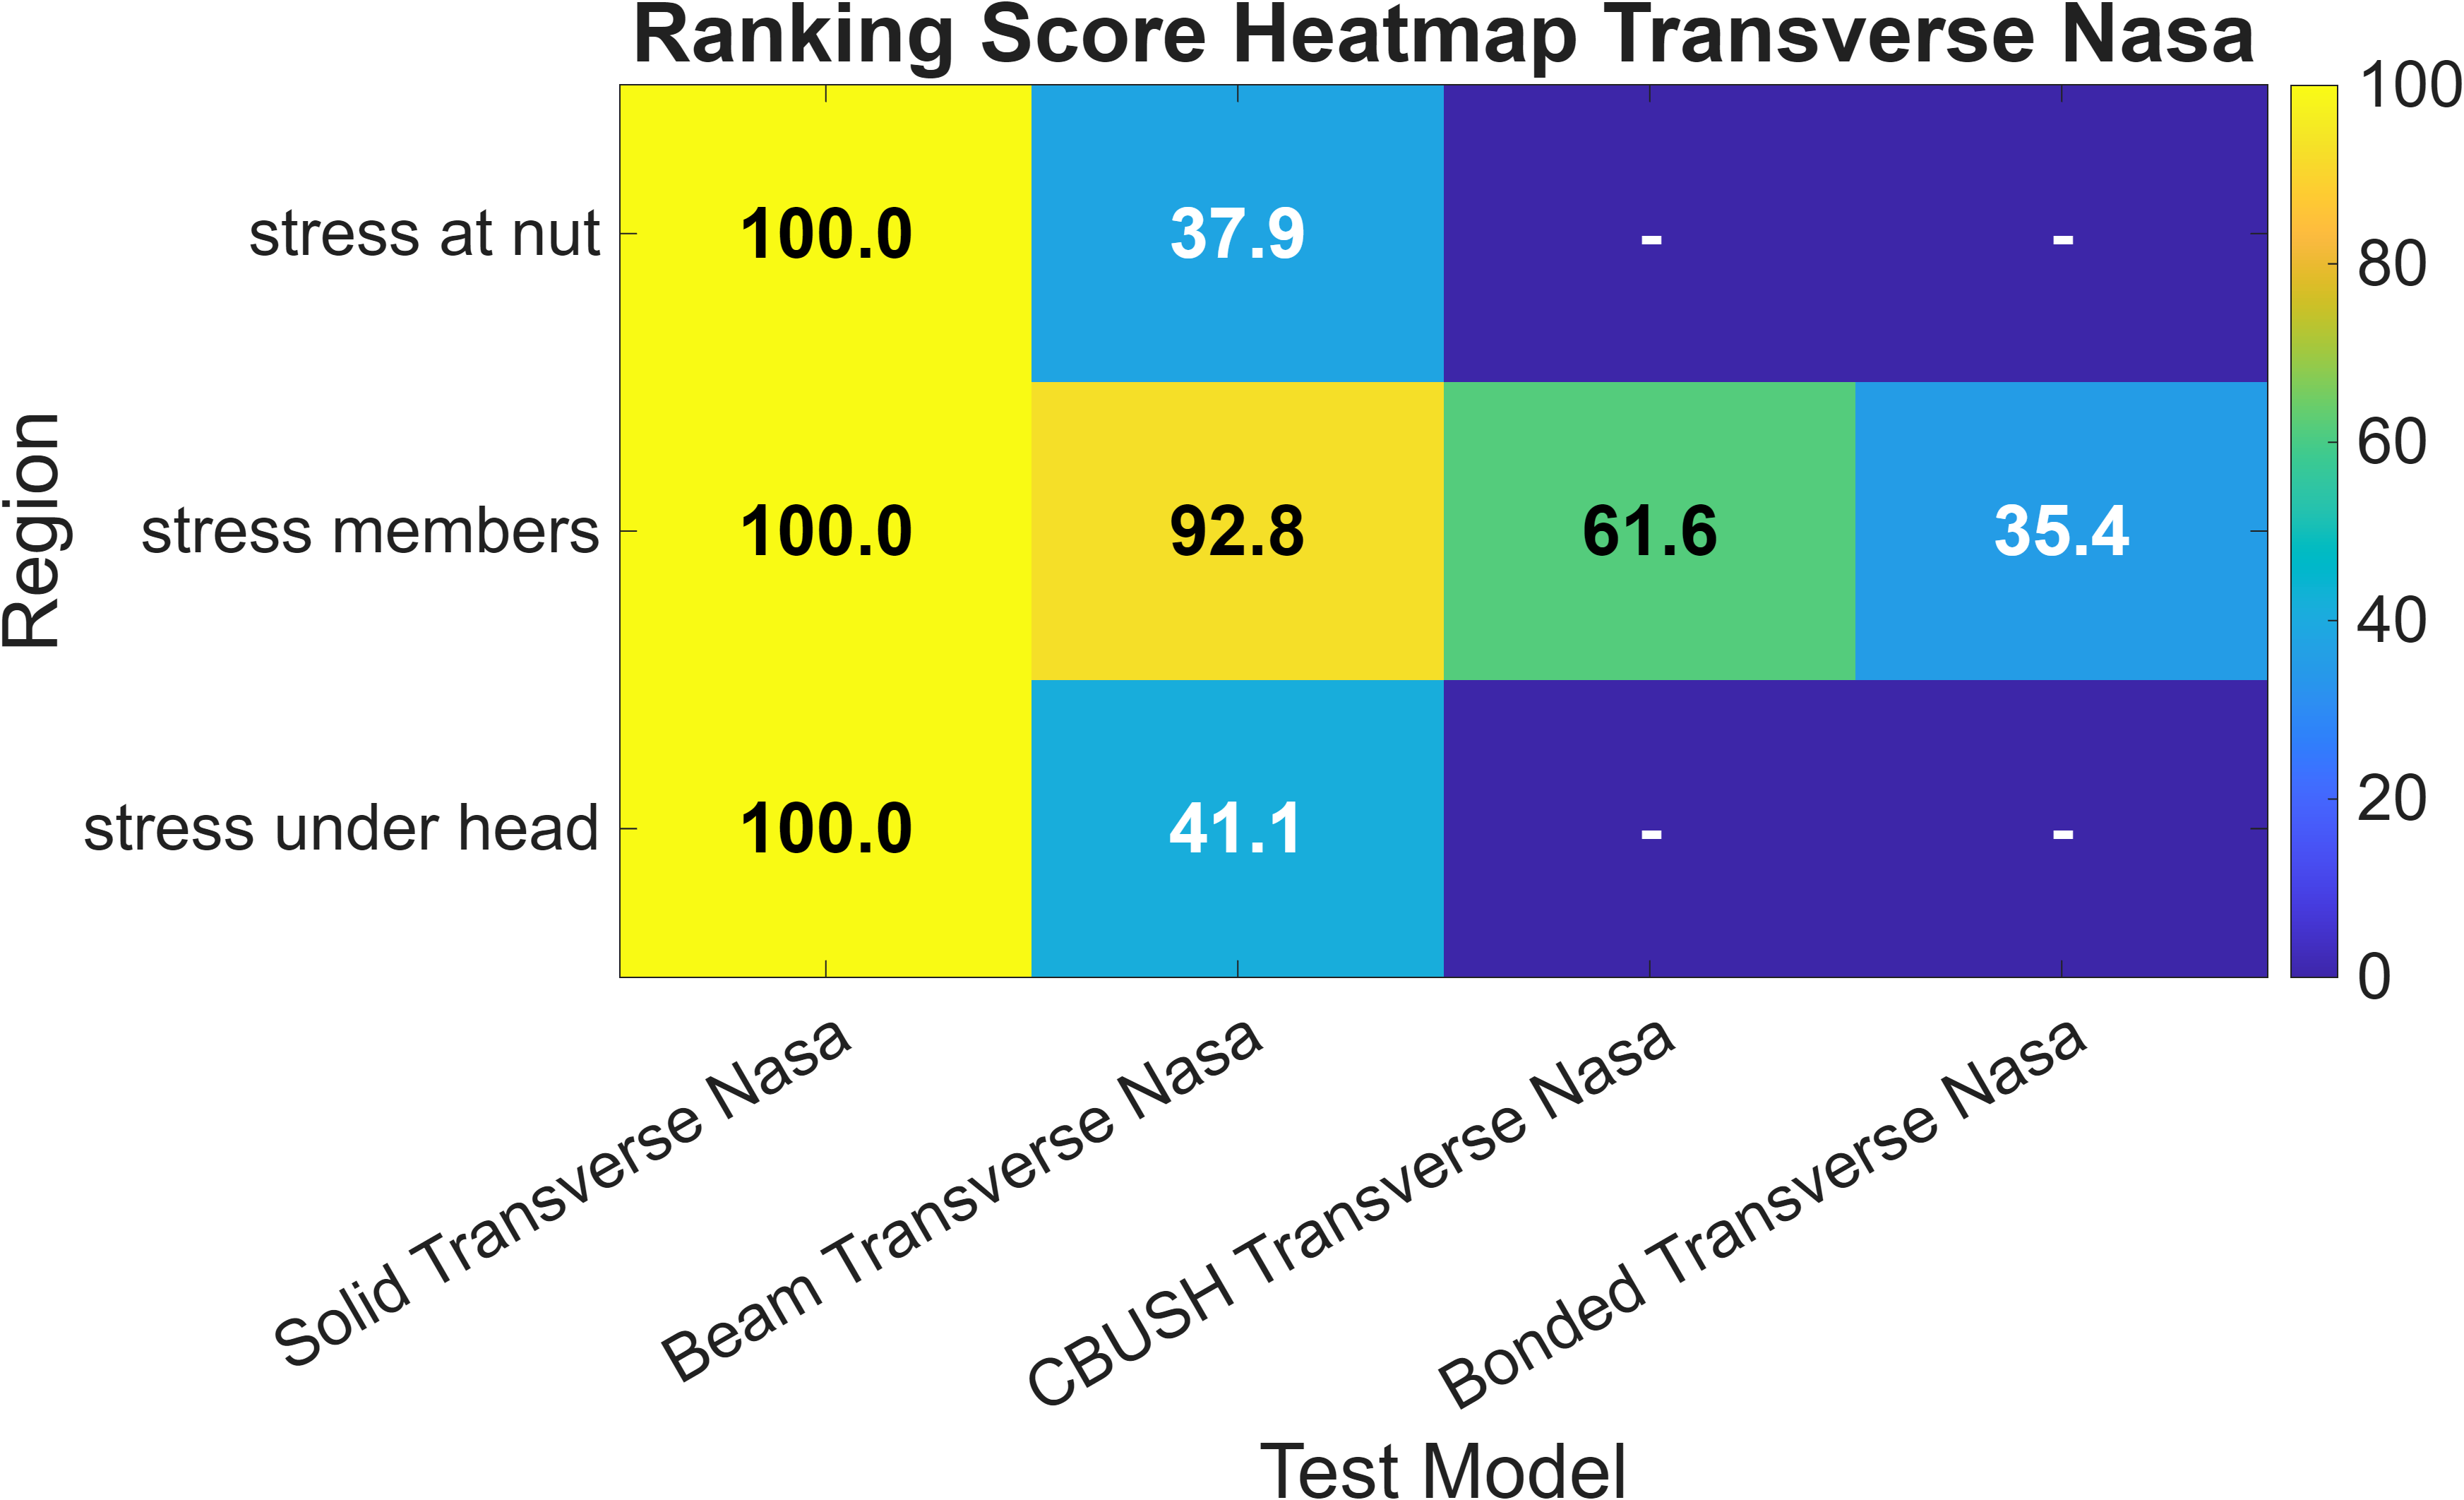
\includegraphics[width=\textwidth]{Transverse Nasa/Transverse Nasa_ranking_heatmap NODEWISE.png}
        \caption{Transverse Loading (shear).}
        \label{fig:NASA_shear_ranking_heatmap_NODEWISE}
    \end{subfigure}
    \begin{subfigure}[b]{0.45\textwidth}
        \centering
        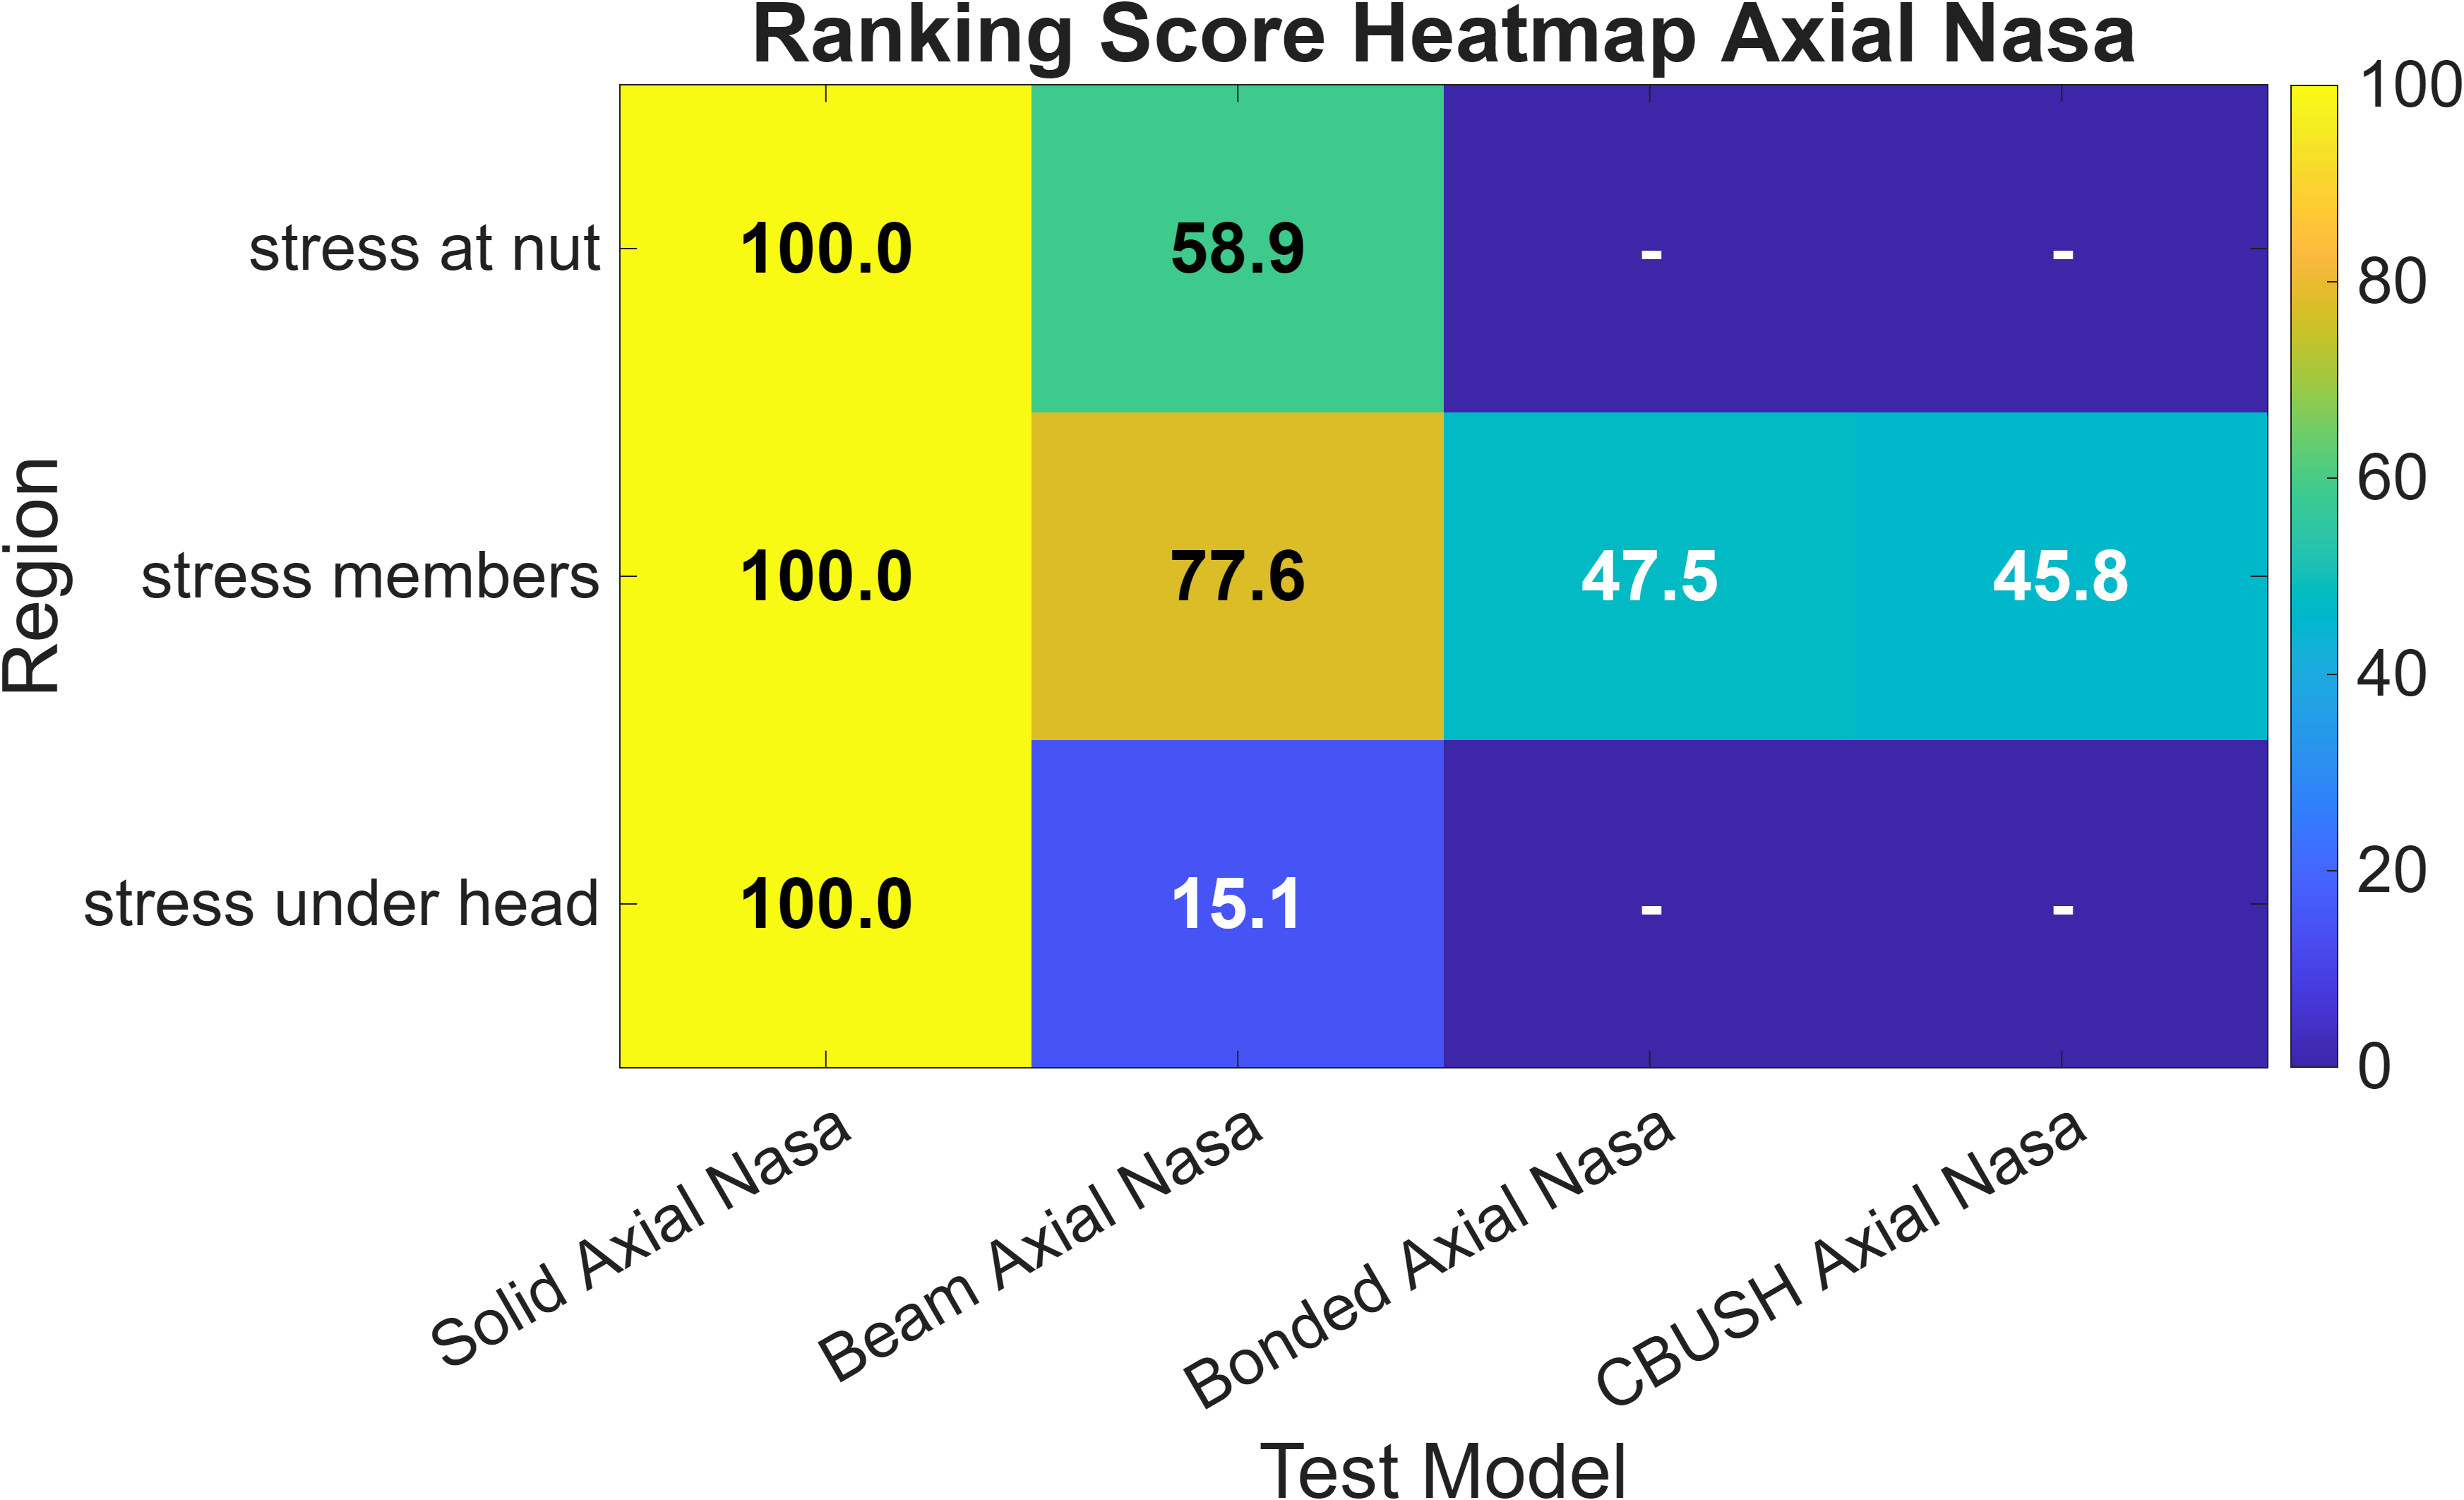
\includegraphics[width=\textwidth]{Axial Nasa/Axial Nasa_ranking_heatmap NODEWISE.png}
        \caption{Axial Loading (bending).}
        \label{fig:NASA_bending_ranking_heatmap_NODEWISE}
    \end{subfigure}
    
    \caption{Ranking Index heatmap. The same trends are visible in the corresponding T43A results, see Appendix \ref{app:T43A_figures}.}
    \label{fig:AccuracyMap_per_region}
\end{figure}


\subsection{Evaluating the cost-metrics}
\begin{table}[H]
    \centering
    \caption{Wall-clock and CPU times for the four bolt representations under the studied benchmark, normalized against the threadless 3D solid reference.}
    \label{tab:WC_CPU}
    \begin{tabular}{lrrrrr}
        \toprule
        \textbf{Model}  & \textbf{Wall-clock [s]} & \textbf{CPU [s]} & \textbf{WC$_n$} & \textbf{CPU$_n$} &\textbf{ Cost $C$} \\
        \midrule
        Solid  & 2236.3 & 8984.1 & 1.00000 & 1.00000 & 100.000 \\
        Beam   & 1878.0 & 8282.7 & 0.83977 & 0.92193 & 88.085 \\
        Bonded & 1289.7 & 4613.0 & 0.57672 & 0.51346 & 54.509 \\
        CBUSH  & 1363.2 & 5388.3 & 0.60959 & 0.59976 & 60.467 \\
        \bottomrule
    \end{tabular}
\end{table}

Two observations follow. First, the simplified models achieve cost reductions: the beam reduces cost by about 12 \%, the bonded and CBUSH representations reduce cost by about 45 \% and 40 \%, respectively, relative to the threadless 3D solid reference. Second, the cost spread between the three simplifications is approximately 34 percent, which is small compared with the spread in their fatigue-related accuracy scores. These cost values feed directly into the Efficiency Ratio (Equation \ref{eq:eta}).

\section{Efficiency Metric} \label{sec:EfficiencyMetric}
Dividing the Ranking Index (Appendix \ref{app:RI_tables}) by the cost gives the efficiency ratios $\eta_{d, i}$ for each direction $d$ and each excitation signal $i$, as seen in Table \ref{tab:cost_efficiency_ratio_summary}:
\begin{table}[H]
    \centering
    \caption{Cost and efficiency ratio for each case and mean efficiency}
    \label{tab:cost_efficiency_ratio_summary}
    \begin{tabular}{lrrrrrr}
        \toprule
        \textbf{Model} & \textbf{$C$} & \textbf{$\eta_{A,NASA}$} & \textbf{$\eta_{T,NASA}$} & \textbf{$\eta_{A,T43A}$} & \textbf{$\eta_{T,T43A}$} & \textbf{$\bar{\eta}$} \\
        \midrule
        Solid & 100.0 & 1.000 & 1.000 & 1.000 & 1.000 & 1.000 \\
        Beam & 88.1 & 0.881 & 1.053 & 0.919 & 0.754 & 0.902 \\
        CBUSH & 60.5 & 0.758 & 1.019 & 0.894 & 1.093 & 0.941 \\
        Bonded & 54.5 & 0.871 & 0.649 & 0.162 & 0.384 & 0.516 \\
        \bottomrule
    \end{tabular}
\end{table}


%The purpose of the Ranking Index is to showcase the possibility of translating results into practical engineering rankings, reminding us of the hypothesis:

% \begin{quote}
%     \textit{\HYP}
% \end{quote}

The efficiency ratio $\eta$ that is visualized in Figure \ref{fig:efficiency} is an internally defined decision metric for this thesis, not a standardized fatigue or \ac{FEA} validation measure. It combines the Ranking Index with normalized solver cost and is therefore sensitive to both the chosen error weights and the chosen cost definition. For this reason, the terms "best agreement" and "best efficiency" are kept separate. A model may agree most closely with the solid reference but still have a lower efficiency ratio than a cheaper model with moderate accuracy. The efficiency ratio should therefore be used as a scoped engineering ranking tool for the present benchmark, not as a universal measure of bolt-model adequacy.

\begin{figure}[H]
    \centering
    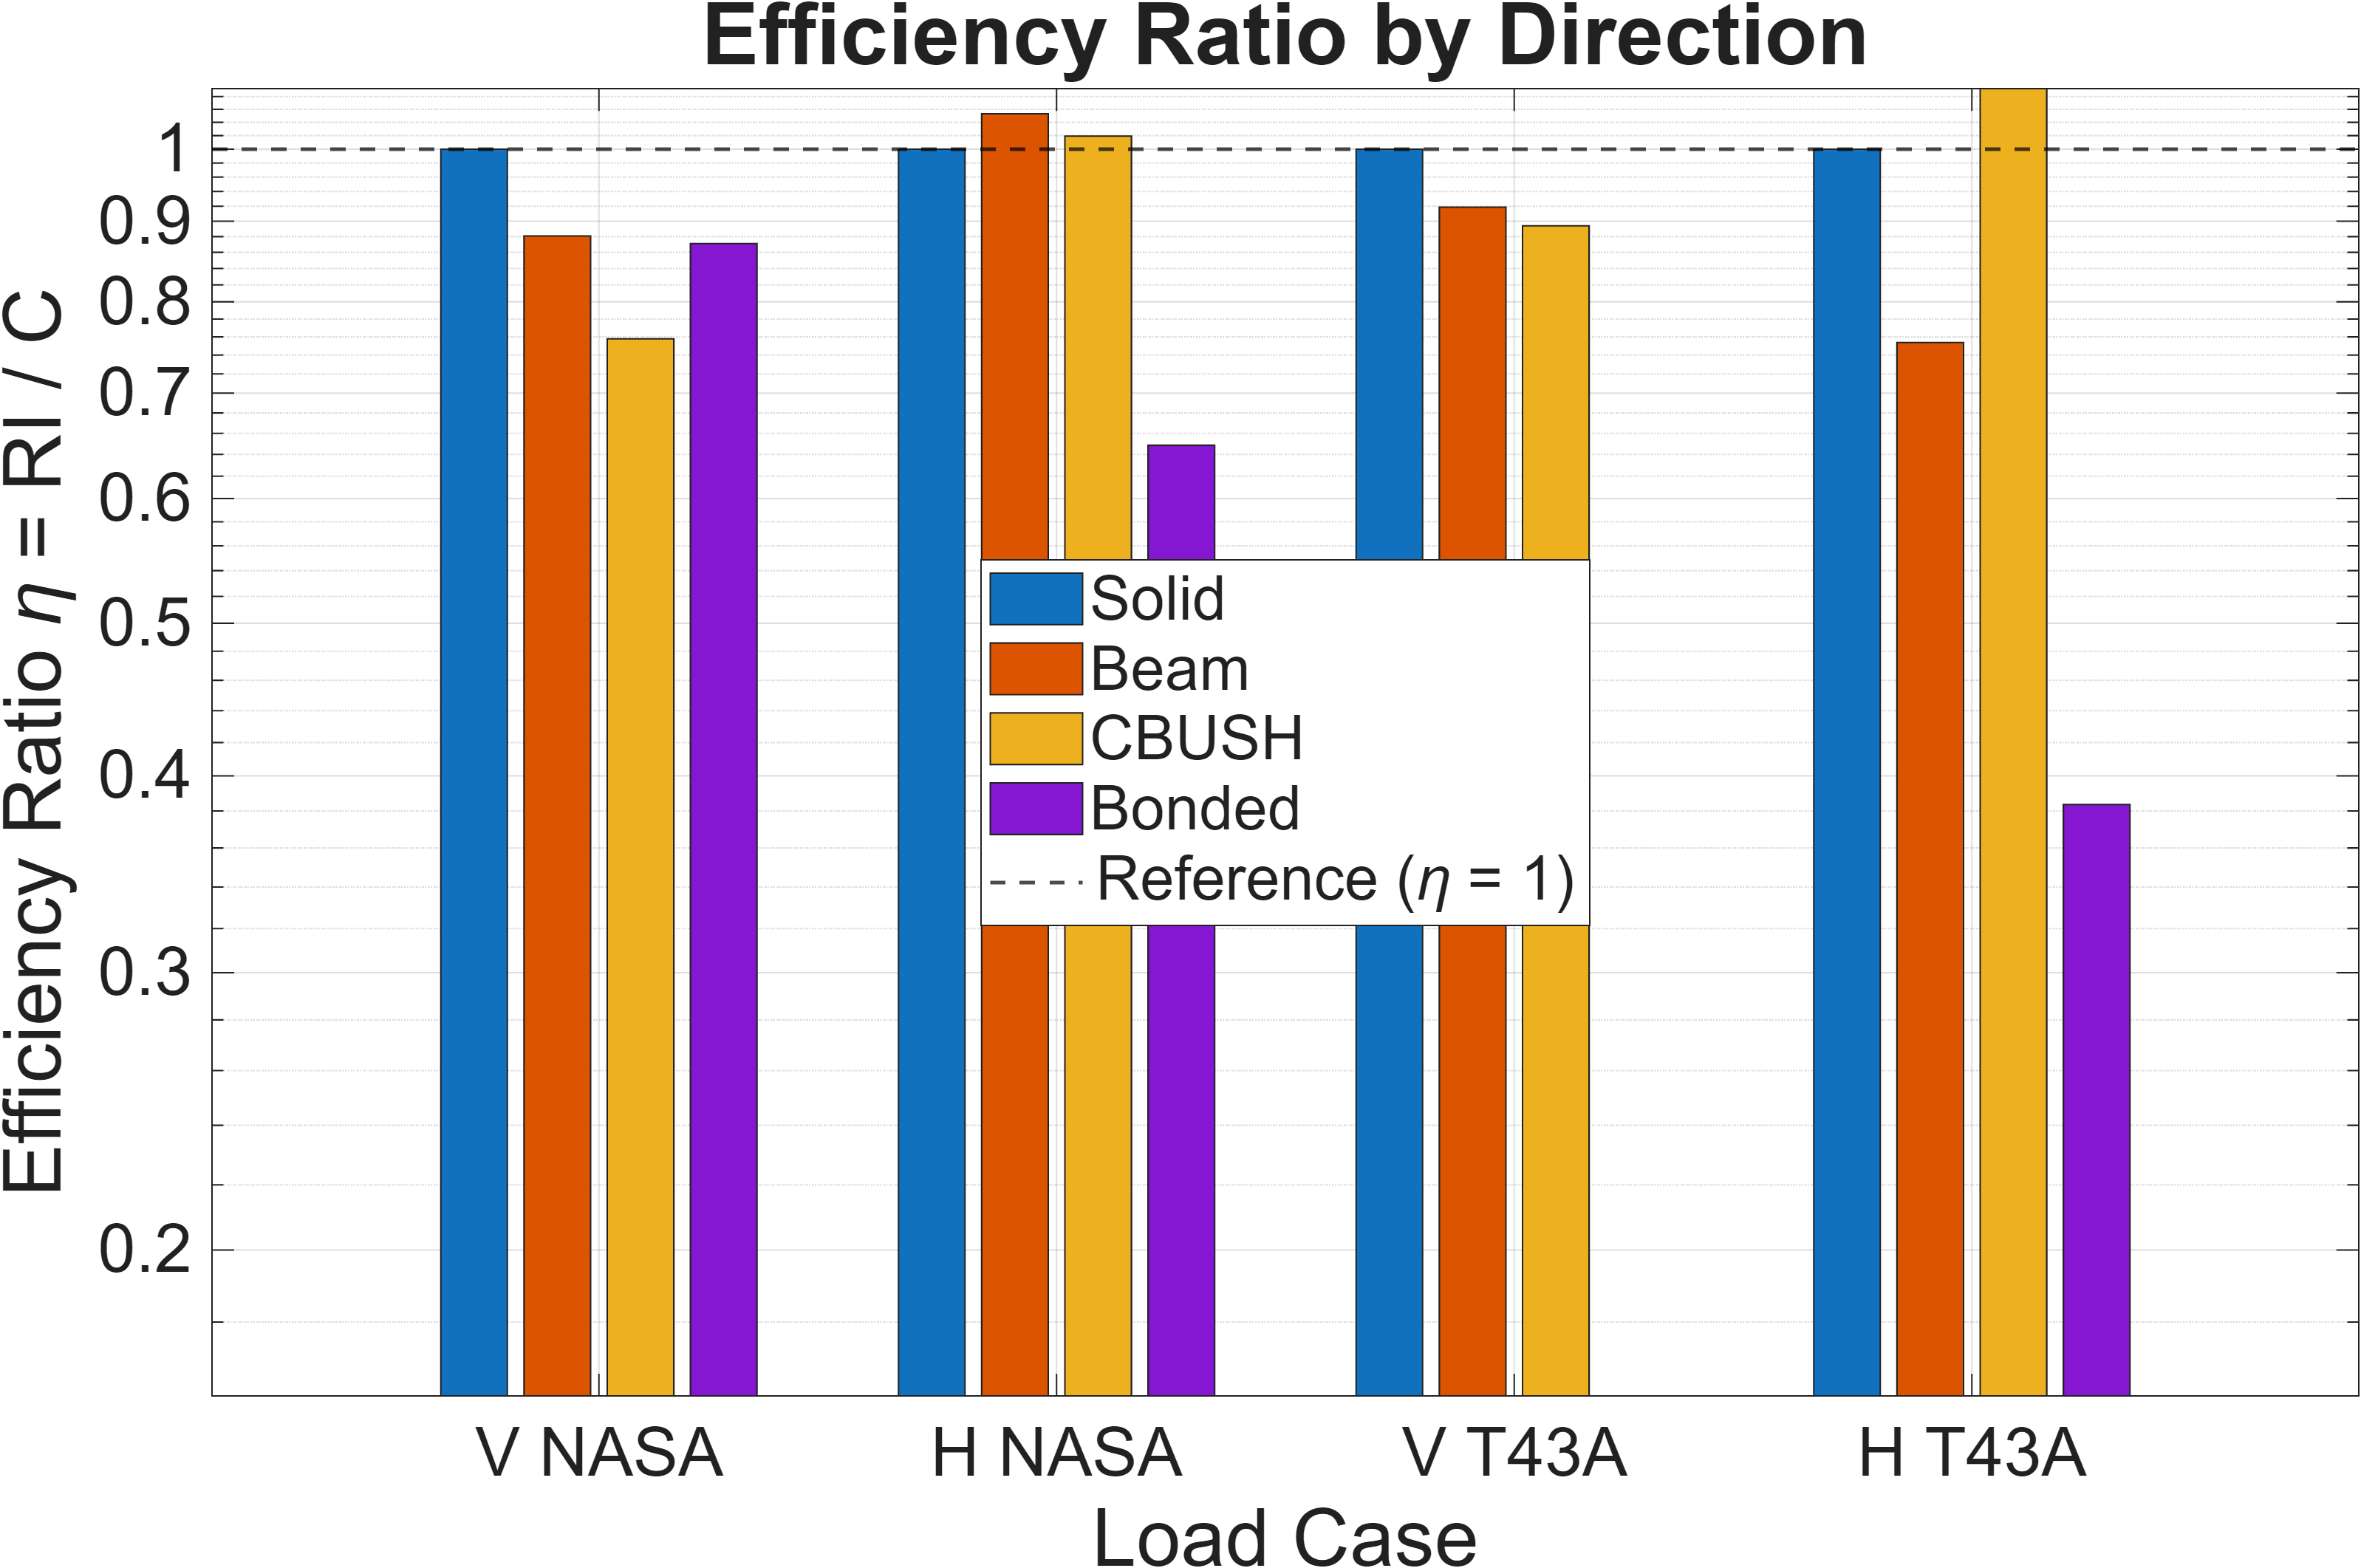
\includegraphics[width=0.75\linewidth]{efficiency_ratio_stress_members_by_direction_and_model NODEWISE.png}
    \caption{Efficiency Ratios for each load case.}
    \label{fig:efficiency}
\end{figure}

The Pareto frontiers in Figure \ref{fig:ParetoNASA} - \ref{fig:ParetoT43A} are also a useful visualization of the same conclusion. With the definition of efficiency that is used in this thesis, not all representations are efficient. It is clear that the bonded and CBUSH models are cheaper, but a major validity boundary should be the set of response quantities each representation can provide.

In each subplot in Figure \ref{fig:ParetoNASA} and \ref{fig:ParetoT43A}, there are two lines: one with the cost metric defined in Section \ref{sec:costMetric} (normalized wall-clock + CPU time) and one that is only normalized wall-clock time, since this is what the engineer will experience. The order of the cost did not change. The order from most expensive to cheapest is in all cases: 1) Solid, 2) Beam, 3) CBUSH, 4) Bonded.

\begin{figure}[H]
    \centering
    \begin{subfigure}[b]{0.45\textwidth}
        \centering
        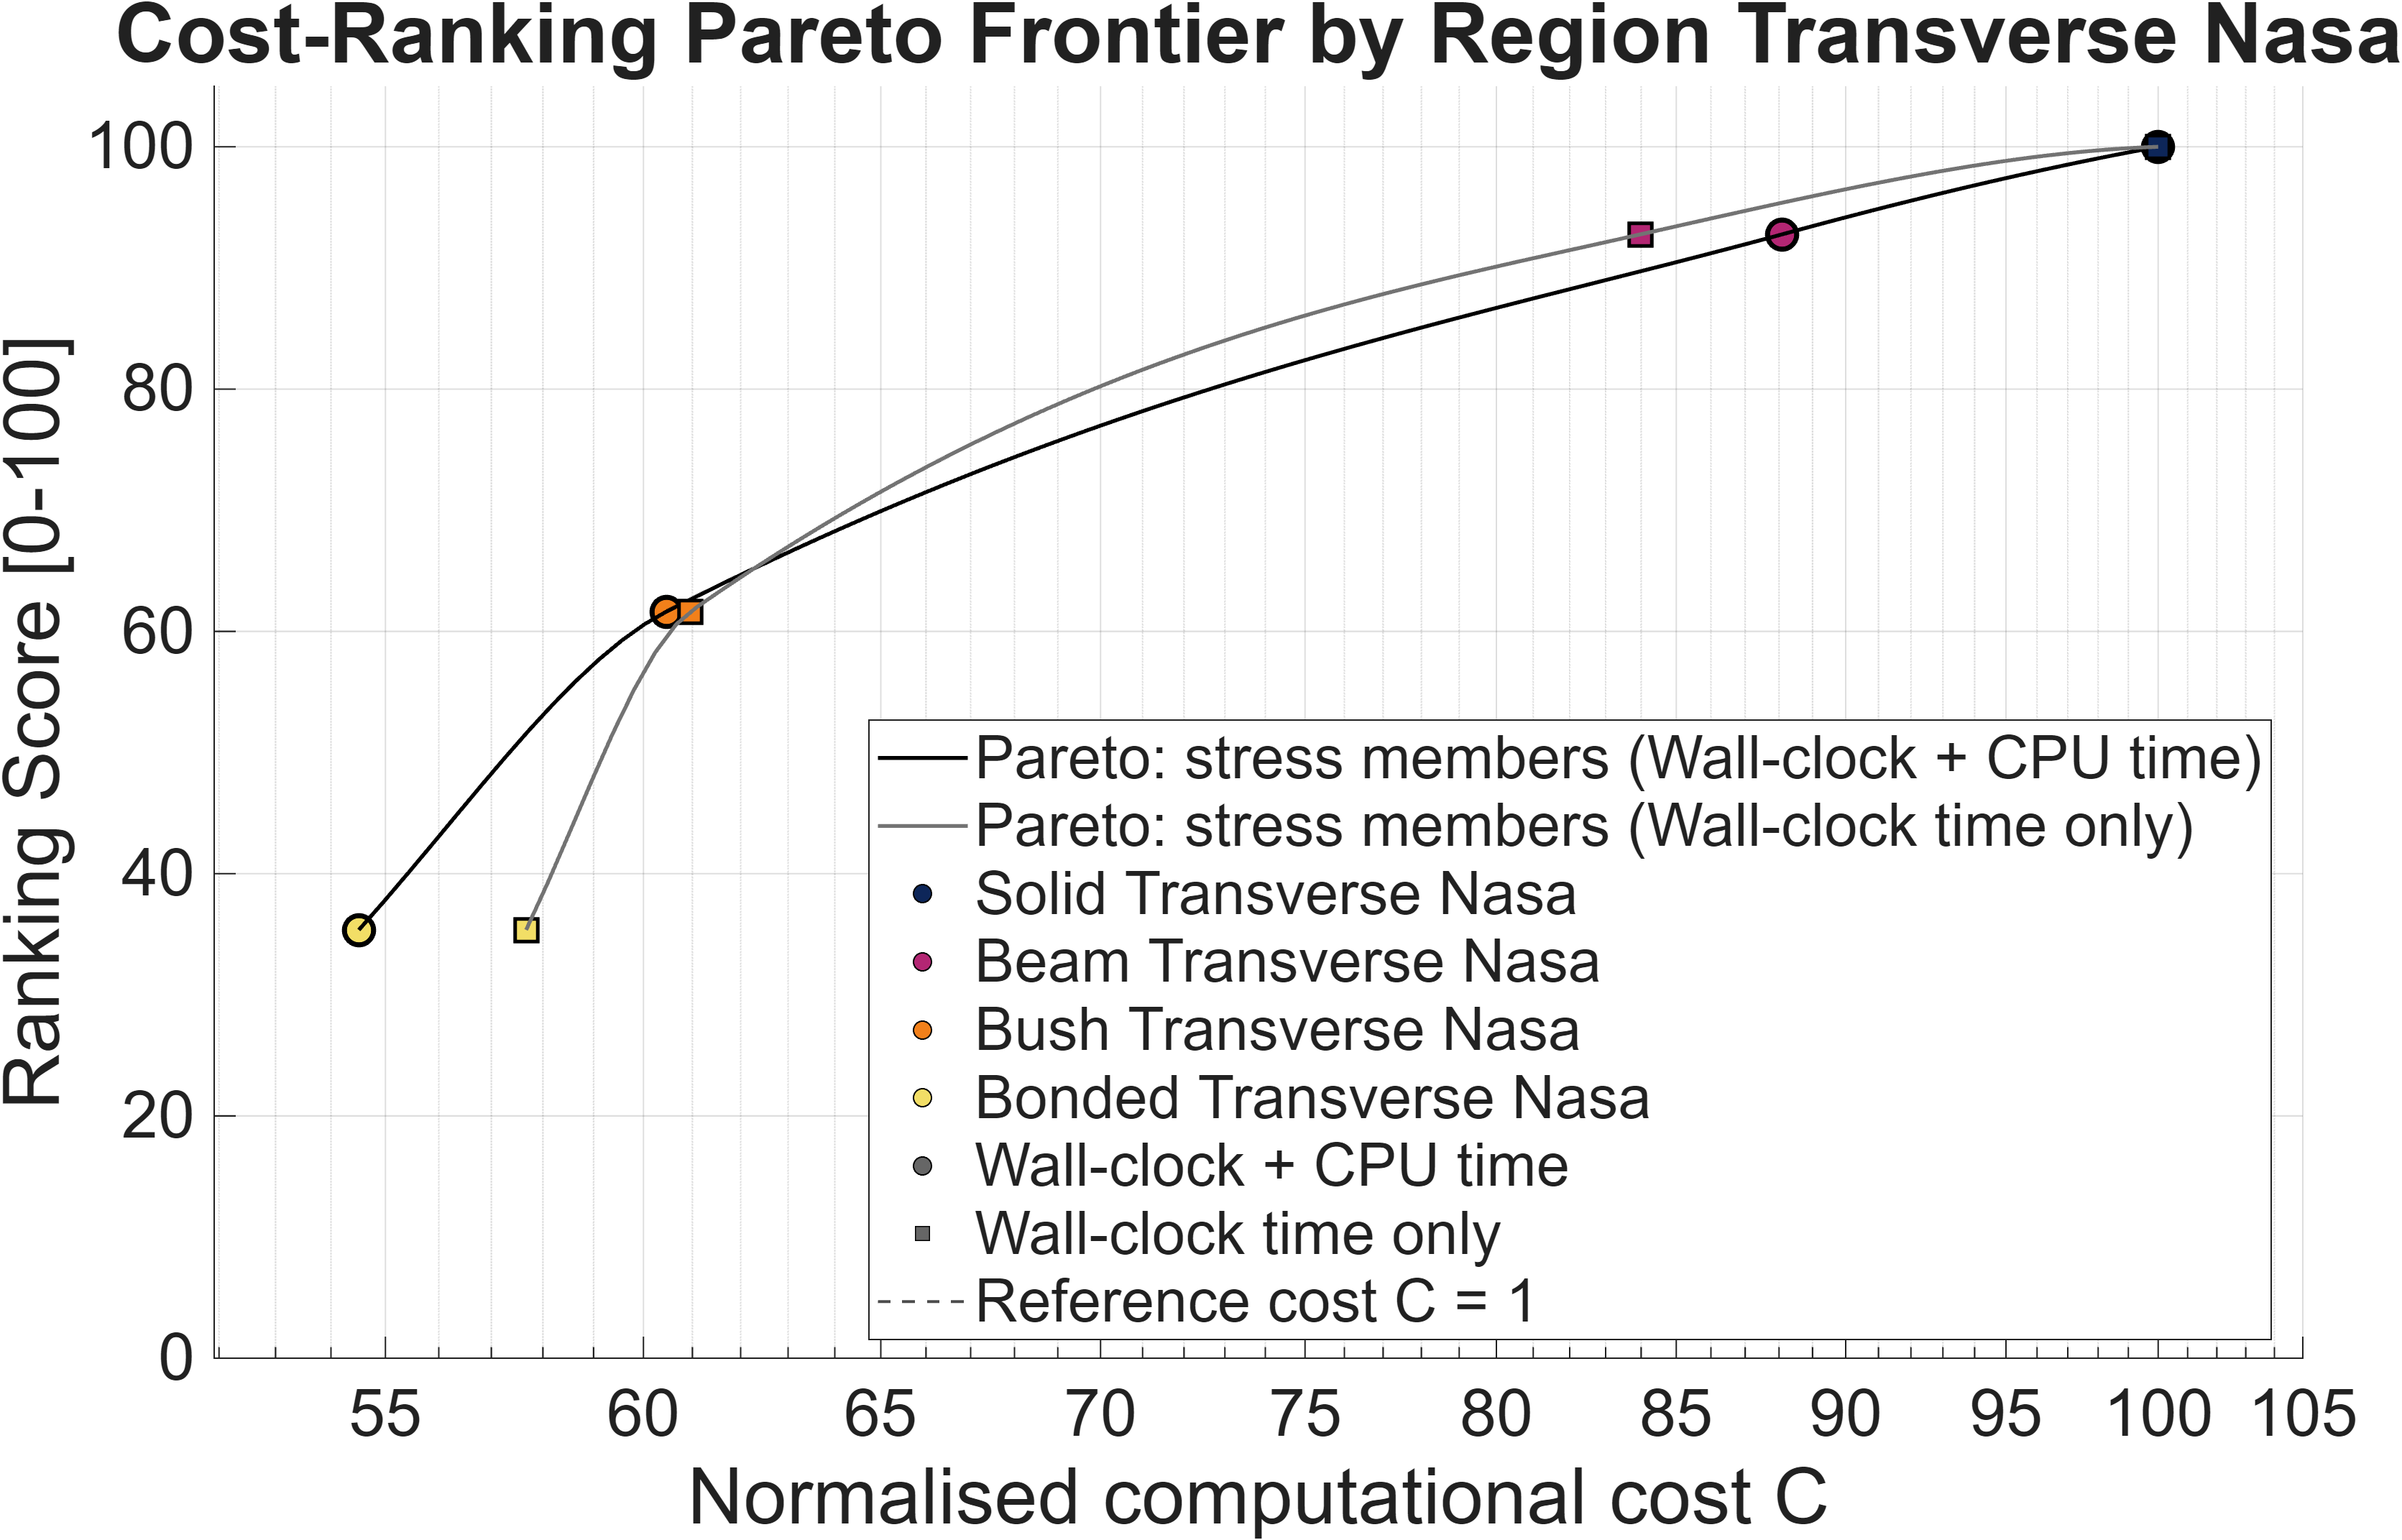
\includegraphics[width=\textwidth]{Transverse Nasa/Transverse Nasa_cost_ranking_pareto_combined NODEWISE.png}
        \caption{Transverse Loading (shear).}
        \label{fig:NASA_shear_cost_ranking_pareto_combined_NODEWISE}
    \end{subfigure}
    \begin{subfigure}[b]{0.45\textwidth}
        \centering
        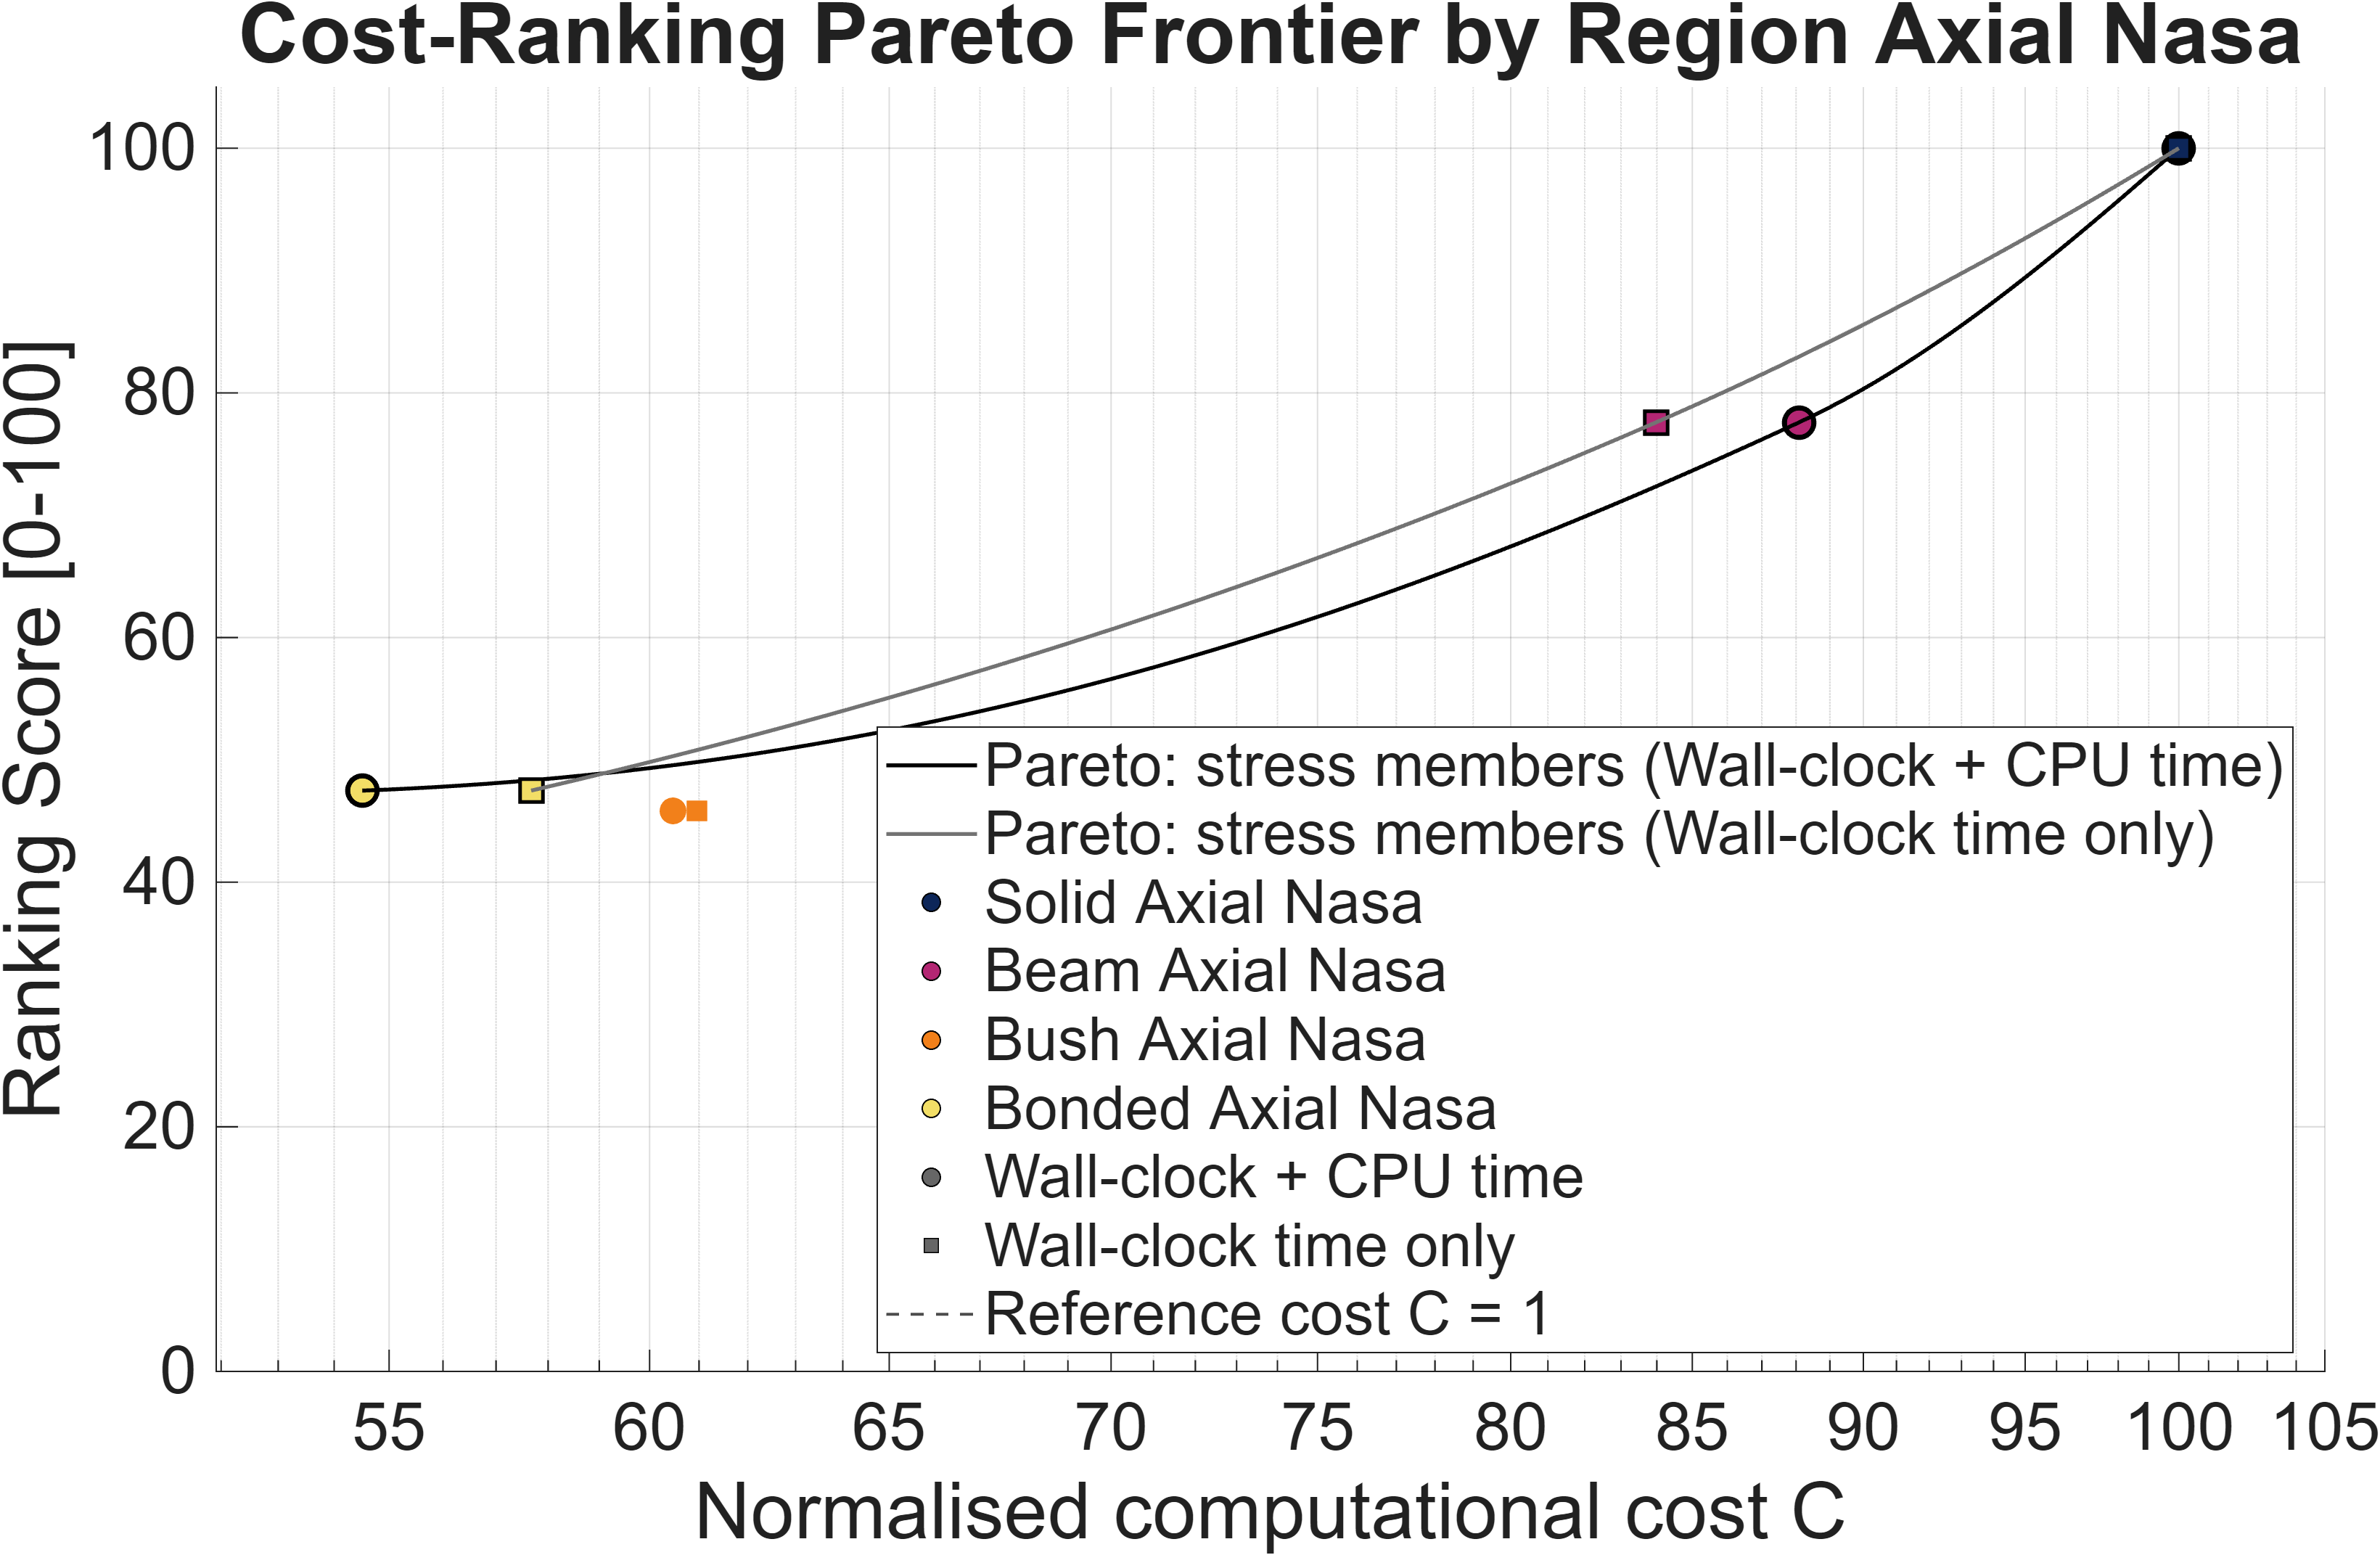
\includegraphics[width=\textwidth]{Axial Nasa/Axial Nasa_cost_ranking_pareto_combined NODEWISE.png}
        \caption{Axial Loading (bending).}
        \label{fig:NASA_bending_cost_ranking_pareto_combined_NODEWISE}
    \end{subfigure}
    
    \caption{Pareto front for the NASA excitation. In the axial (b), the bush is an inefficient choice.}
    \label{fig:ParetoNASA}
\end{figure}

\begin{figure}[H]
    \centering
    \begin{subfigure}[b]{0.45\textwidth}
        \centering
        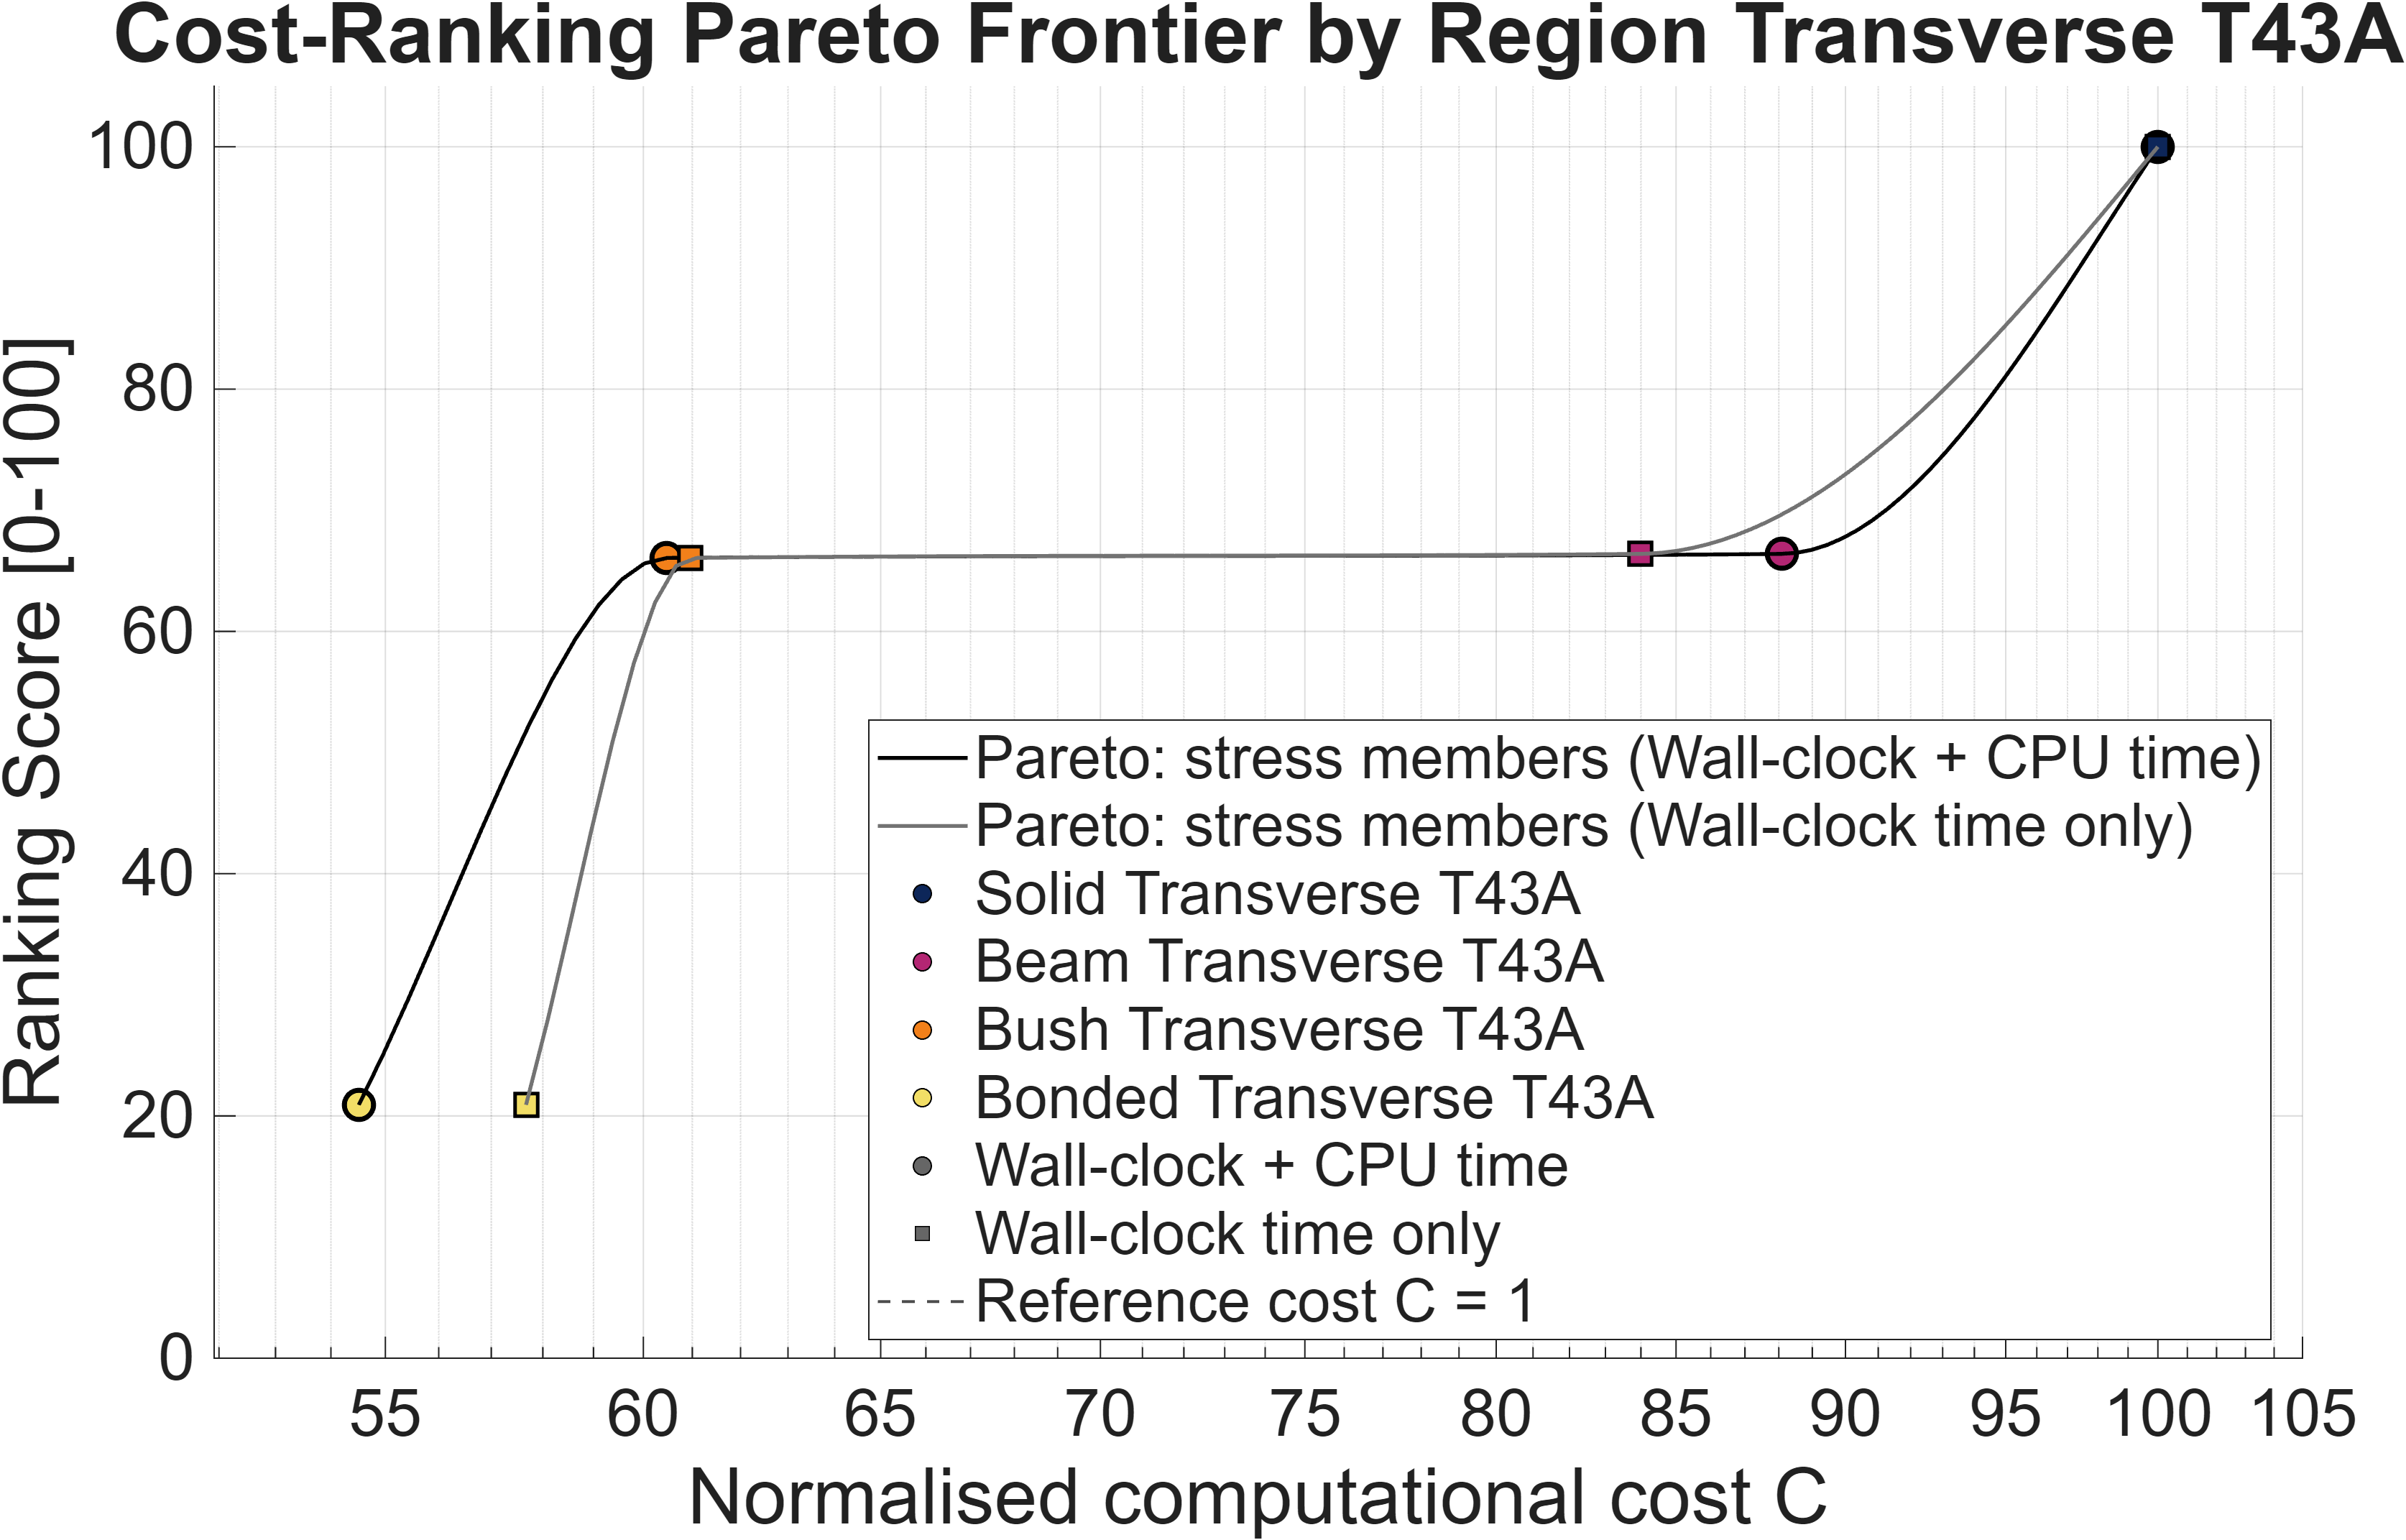
\includegraphics[width=\textwidth]{Transverse T43A/Transverse T43A_cost_ranking_pareto_combined NODEWISE.png}
        \caption{Transverse Loading (shear).}
        \label{fig:T43A_shear_cost_ranking_pareto_combined_NODEWISE}
    \end{subfigure}
    \begin{subfigure}[b]{0.45\textwidth}
        \centering
        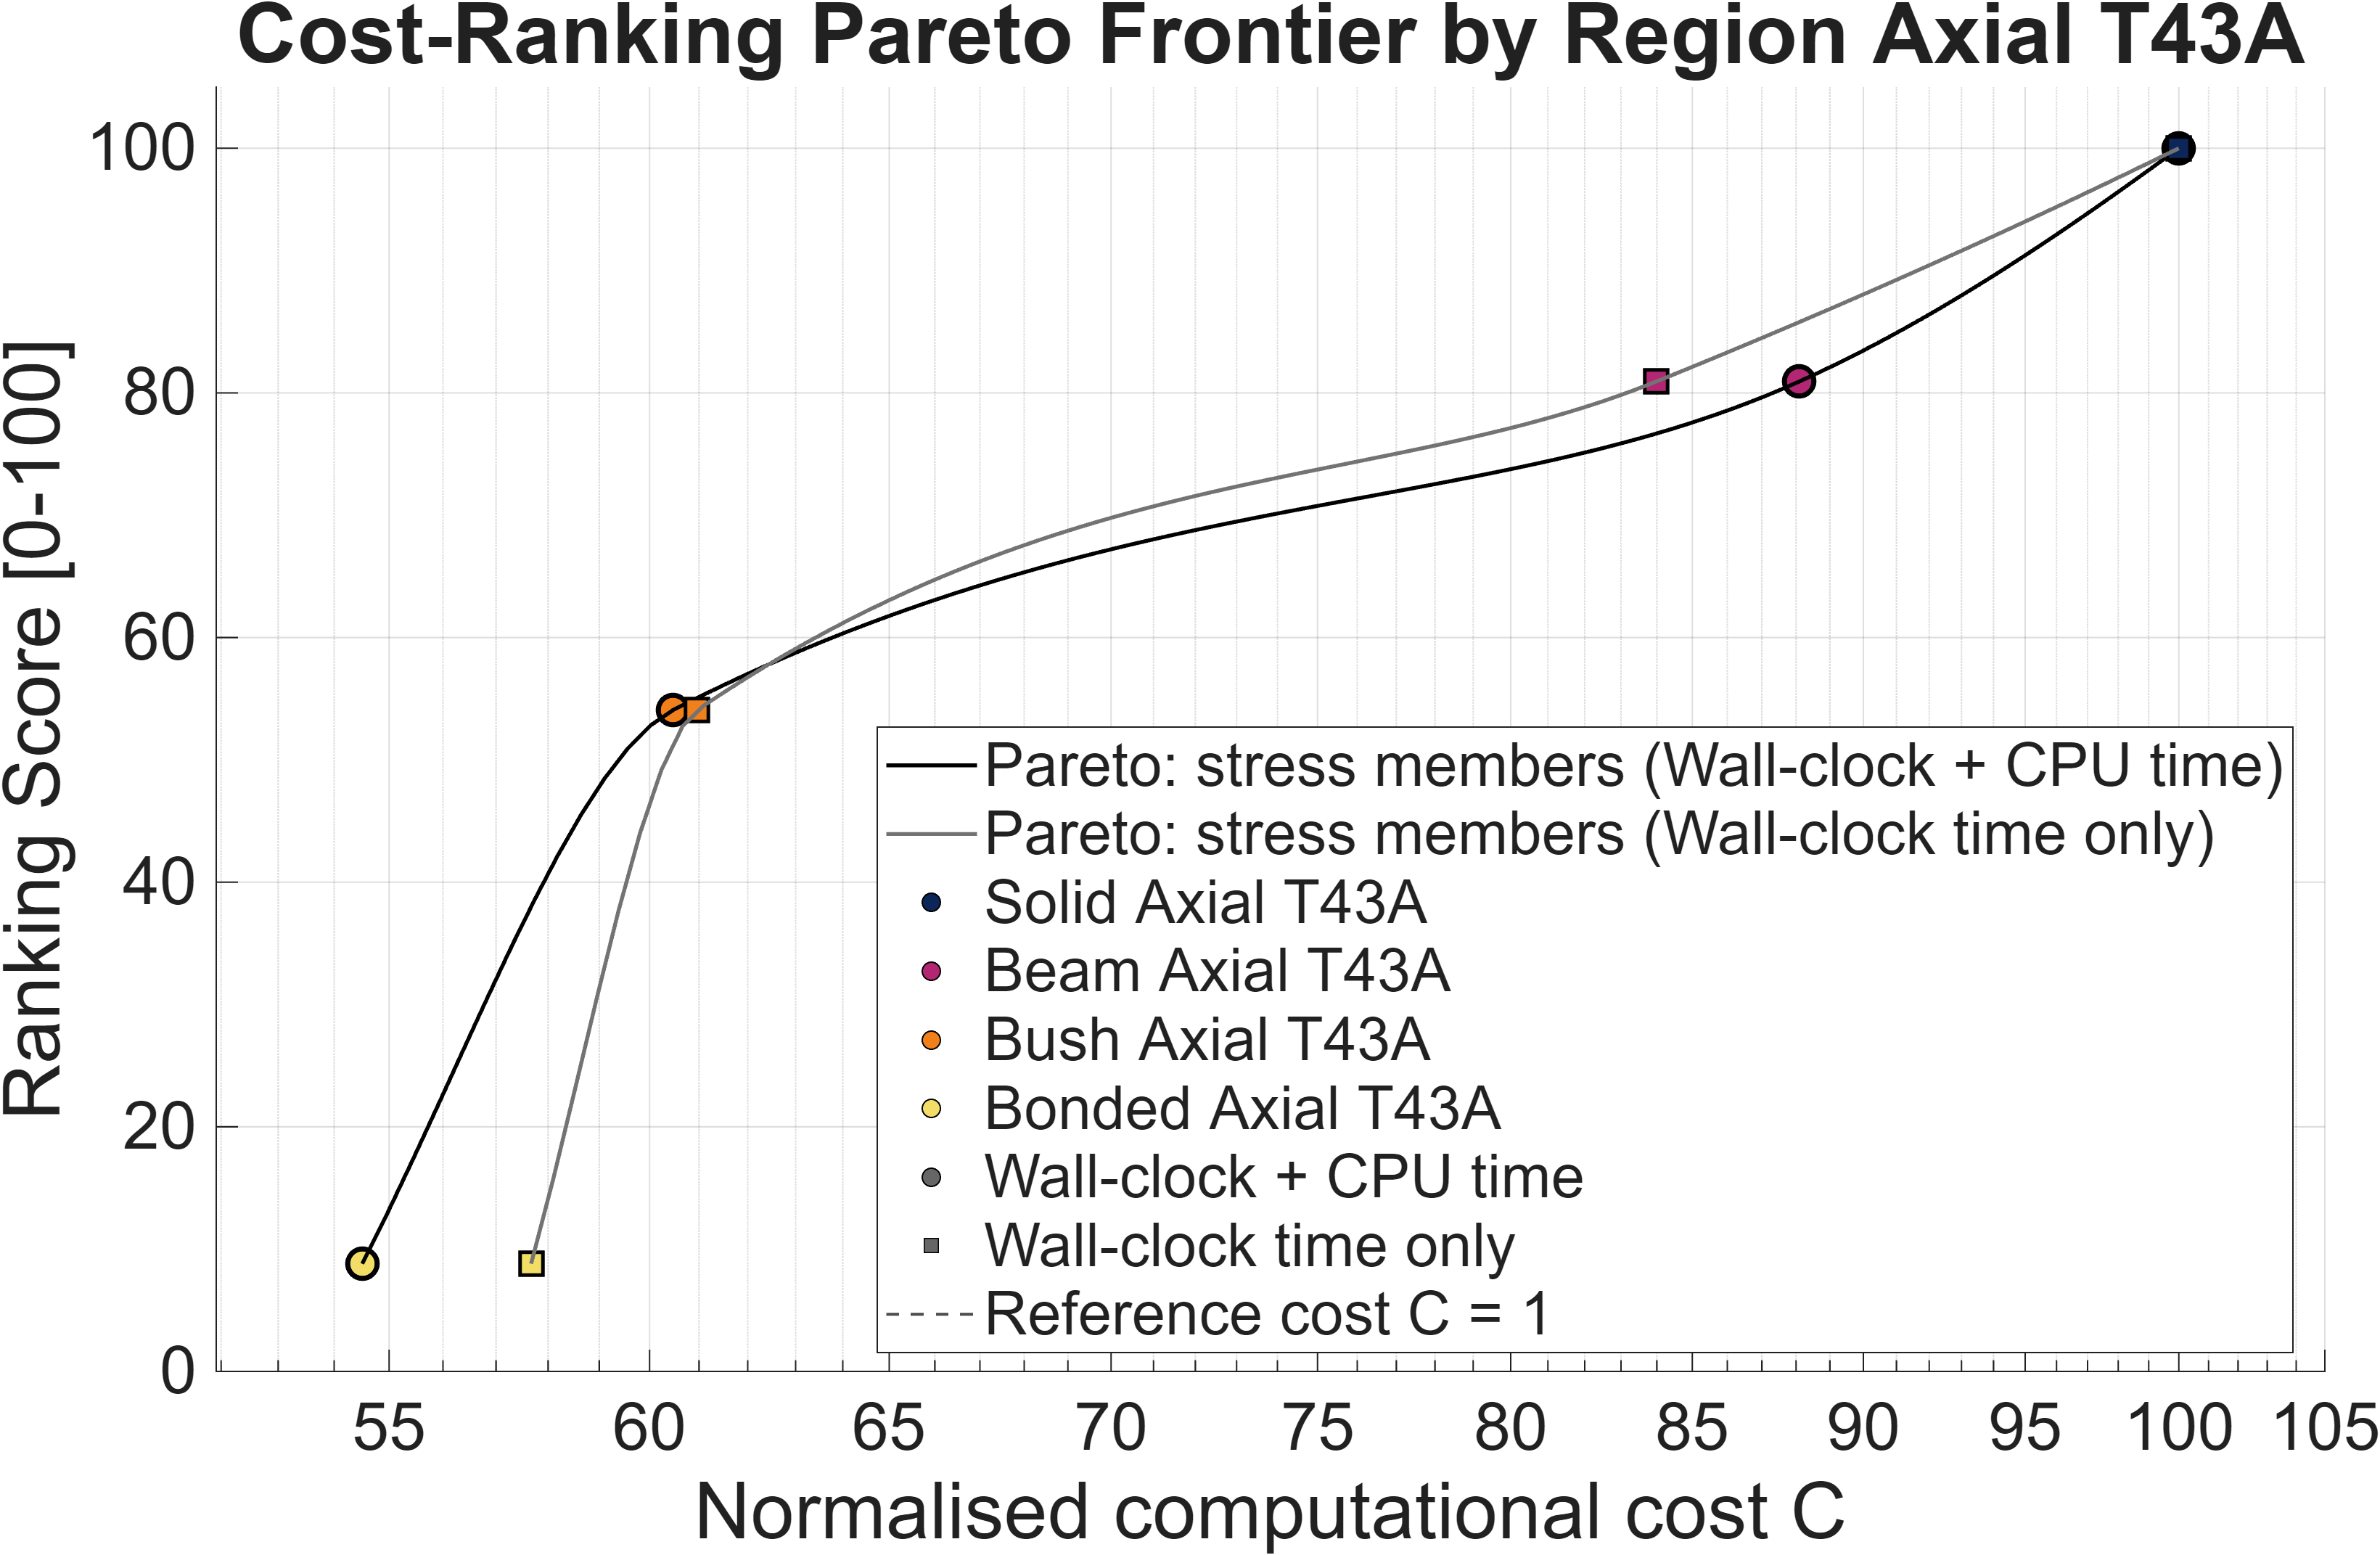
\includegraphics[width=\textwidth]{Axial T43A/Axial T43A_cost_ranking_pareto_combined NODEWISE.png}
        \caption{Axial Loading (bending).}
        \label{fig:T43A_bending_cost_ranking_pareto_combined_NODEWISE}
    \end{subfigure}
    
    \caption{Pareto front for the T43A excitation.}
    \label{fig:ParetoT43A}
\end{figure}


\newpage
\section{Designing the Guidelines}
The aim is to fill the existing knowledge gap by developing evidence-based guidelines. These guidelines are intended to help engineers optimize the selection of the \ac{FEA} method for fatigue analysis by balancing accuracy and computational cost. To make the guidelines practically useful for a computational engineer before any simulations are run, and without requiring knowledge of the exact "truth" for the specific assembly, the guidelines rely on pre-established benchmarks.

\begin{figure}[H]
    \centering
    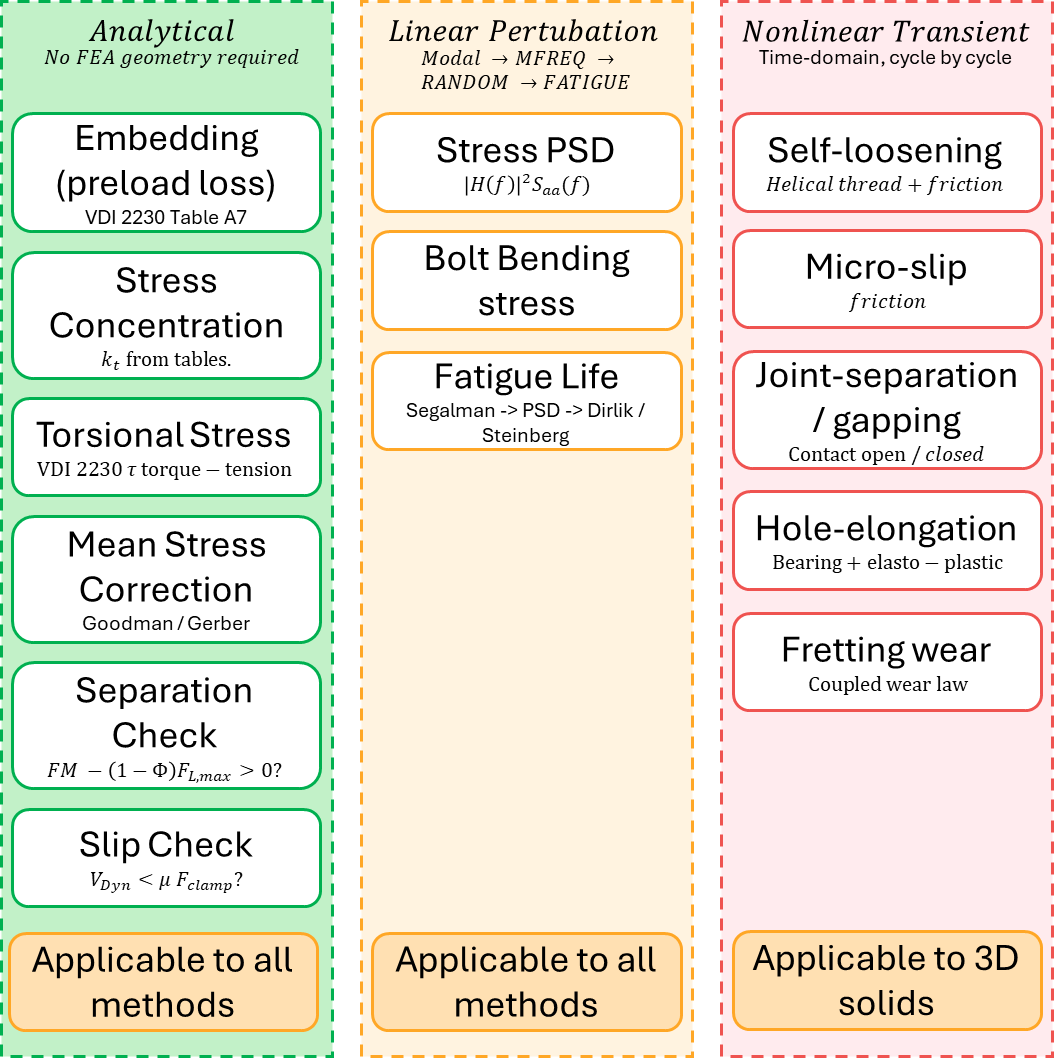
\includegraphics[width=0.75\linewidth]{Figures/columns.png}
    \caption{Catalog of the analysis necessary for different phenomena, sorted by \textit{Analytical} (least expensive), \textit{Linear Perturbation} (more expensive), and \textit{Nonlinear Transient} (most expensive).}
    \label{fig:PhenomenaColumns}
\end{figure}

Once these guidelines are established, engineers can confidently select the most suitable bolt representation and analysis type in advance, based on project parameters, without needing to perform validation themselves.
\newpage
\subsection{How the Guidelines should be used / Practical Implications for Engineering Work}
The engineer first defines the practical limitations, which are not a part of the present guidelines, but should include questions such as:
\begin{enumerate}
    \item Available time: How much pre-processing and solver time is permitted?
    \item Required precision level: What tolerance of deviation from the reference is acceptable for the specific component? Which metric is used from the truth (stress, fatigue life, modes, ...)?
    \item Maturity of input data: How detailed are the current design and load data?.
\end{enumerate}

Once these constraints are defined, the engineer must specify which phenomena are expected and which are critical to extract from the \ac{FEA}. The guidelines provide a matrix that specifies which simplified models can capture specific phenomena. For example, if the engineer needs to capture self-loosening, the guidelines state that only the expensive, fully threaded, three-dimensional solid model is needed for a nonlinear transient analysis. If the engineer only needs global behavior and fatigue failure of the bolt is not crucial, a bonded surface might be sufficient, along with a linear frequency analysis.

For all simplified representations, the error spectra show their largest deviations at the eigenfrequencies of the structure. One of the parameters that can be used to determine the validity of a simplified method would be whether an eigenfrequency is excited by the input \ac{PSD} at all. If, for example, a structure has its first eigenfrequency at 100 Hz but is only excited with a \ac{PSD} defined up to 50 Hz, the global damage of the structure would be within the same order of magnitude as the reference model, even with the most simplified method, since no major resonance is activated. Still, not all phenomena can be captured with any single simplified method. Even if the global response is within a validity boundary, it would be impossible to evaluate fatigue failure of the bolt in computation method A, for example, since it has no geometry.

The global stress error can always be lower with a CBUSH than with a beam in the 1D model, but it would require analytically computed stiffnesses. These analytical calculations are computationally cheap but require some understanding of how to use the standards. A tool that takes input and returns the analytical stiffnesses would be useful.

A conclusion can be drawn that the engineer must choose the right tool for the job - the applicability of a bolt model depends on the quantity of interest and on the extraction region.

If the aim is to estimate the dynamic stress and fatigue response of clamped members at reduced computational cost, the beam model provides the best trade-off among the simplified alternatives considered in this thesis under both loading directions.

If, on the other hand, the aim is to assess local bolt stresses or bolt fatigue, the beam model provides moderate accuracy under transverse (shear) loading but poor accuracy under axial (bending) loading in the under-head region. In all cases, a solid bolt representation is required when accurate local bolt stresses are required.

The results of this thesis translate into concrete recommendations for engineers who perform \ac{FEA} of bolted joints under random-vibration fatigue. These recommendations are valid within the scope stated in Section \ref{sec:limitations}, and are designed to support, not replace, engineering judgment.

One clear recommendation is to choose the response quantity before choosing the bolt representation. The phenomenon-method matrix (Table \ref{tab:phenomenaMethodMatrix}) and the decision flowchart (Figure \ref{fig:decisionTree}) walk the engineer from the engineering question to the minimum adequate model. Before running a simulation, trace the path through the flowchart for the intended analysis. When the flowchart directs a case to a fidelity that the planned model doesn't meet, you have two options: 1) increase the model's fidelity, or 2) accept that certain phenomena will be excluded from the model's analysis. This approach is quicker and more cost-effective than discovering the model's limitations after running a full stress \ac{PSD} analysis.

\subsection{Limitations of the conclusions} 
The conclusions drawn above hold within the following bounds:
\begin{enumerate}
    \item Geometric scope: a single-bolt benchmark was used (Chapter \ref{chp:method}). The present model does not capture multi-bolt patterns, flange joints, and lap joints. The ranking of simplified models established here should therefore be revalidated on multi-bolt geometries before it is applied to a production assembly.
    \item Dynamic scope: a linear perturbation frequency-domain analysis was used. The contact state is frozen at the end of the initial nonlinear static preload step. This means that contact-status dependent phenomena, such as macro-slip and contact opening, are not represented. For excitation amplitudes high enough to drive slipping in the joint, a fully nonlinear transient analysis is required, and the simplified model ranking established here cannot be assumed to still be valid in that sort of analysis.
    \item Excitation scope: Two standardized excitation profiles were tested. The NASA -STD-7001B Workmanship profile and the MIL-STD-810G T43A profile. The agreement between Dirlik and Steinberg and the spread of the Ranking Index were found to depend on the signal.
    \item Validation scope: the reference model that is used is a 3D solid bolt without threads, not a physical test. The Ranking Index is therefore relative to a higher-fidelity model rather than to the actual measured fatigue life.
    \item Load-direction scope: each load case is applied to a single axis at a time. Multiaxial excitation was not tested.
\end{enumerate}

\newpage
\section{The Guidelines} \label{sec:Deliverables}
The guidelines in this thesis are built from two deliverables that together answer the research question, but that play different roles:
\begin{enumerate}
    \item a phenomenon-method matrix (Table \ref{tab:phenomenaMethodMatrix}), derived from theory and literature, that indicates the minimum modeling fidelity and analysis type that is required to capture a given physical phenomenon, and
    \item a decision flowchart (Figure \ref{fig:decisionTree}) that walks the engineer from an engineering question to a recommended \ac{FE} bolt representation and analysis type.
\end{enumerate}

The computational results, by themselves, do not establish the full matrix. Rather, they provide quantitative support for the fatigue- and stress-related parts of the decision logic in the studied benchmark, and especially where the engineering question concerns clamped-member response vs local-bolt response under the chosen loading conditions.

The results show that the target question should drive the model selection. When the engineering objective is global response or stress behavior in the clamped members, lower-cost models can provide sufficiently accurate results at a considerably lower computational cost. However, when the objective is to assess local bolt stresses or fatigue-critical regions of the bolt, detailed solid bolt models are necessary, as simplified models do not accurately reproduce these stresses.

\begin{landscape}
\begin{table}[H]
    \centering
    \caption{Phenomenon-method matrix.}
    \label{tab:phenomenaMethodMatrix}
    \begin{tabular}{lccccc}
        \toprule
         Phenomenon / quantity & Bonded & Beam & CBUSH & Threadless Solid & Threaded Solid \\
        \midrule
         Global / clamped-member stress    & \textbullet & \textbullet & \textbullet & \textbullet & \textbullet \\
         Preload effect on global response & \textbullet & \textbullet & \textbullet & \textbullet & \textbullet \\
         Bolt axial force                  &             & \textbullet & \textbullet & \textbullet & \textbullet \\
         Bolt bending (significance check) &             & \textbullet & \textbullet & \textbullet & \textbullet \\
         Bolt shear                        &             & \textbullet & \textbullet & \textbullet & \textbullet \\
         Under-head fillet stress          &             &             &             & \textbullet & \textbullet \\
         Thread-root stress concentration  &             &             &             & (SCF post-proc.) & \textbullet \\
         Hole elongation                   &             &             &             & \textbullet\,(plastic) & \textbullet\,(plastic) \\
         Slipping (binary check)           & (analytical) & (analytical) & (analytical) & \textbullet & \textbullet \\
         Slipping (full resolution)        &             &             &             & \textbullet\,(frictional contact) & \textbullet\,(frictional contact) \\
         Self-loosening (Stage II)         &             &             &             &             & \textbullet\,(nonlinear transient) \\
         Residual torsional bolt stress    &             &             &             &             & \textbullet\,(nonlinear transient) \\
        \bottomrule
    \end{tabular}
\end{table}

The cheapest model capable of capturing the phenomenon is marked with \textbullet. Methods above it in fidelity also work. An empty cell means the method cannot capture the phenomenon at a useful level, even with post-processing.

\end{landscape}

\newpage


\begin{figure}[H]
    \centering
    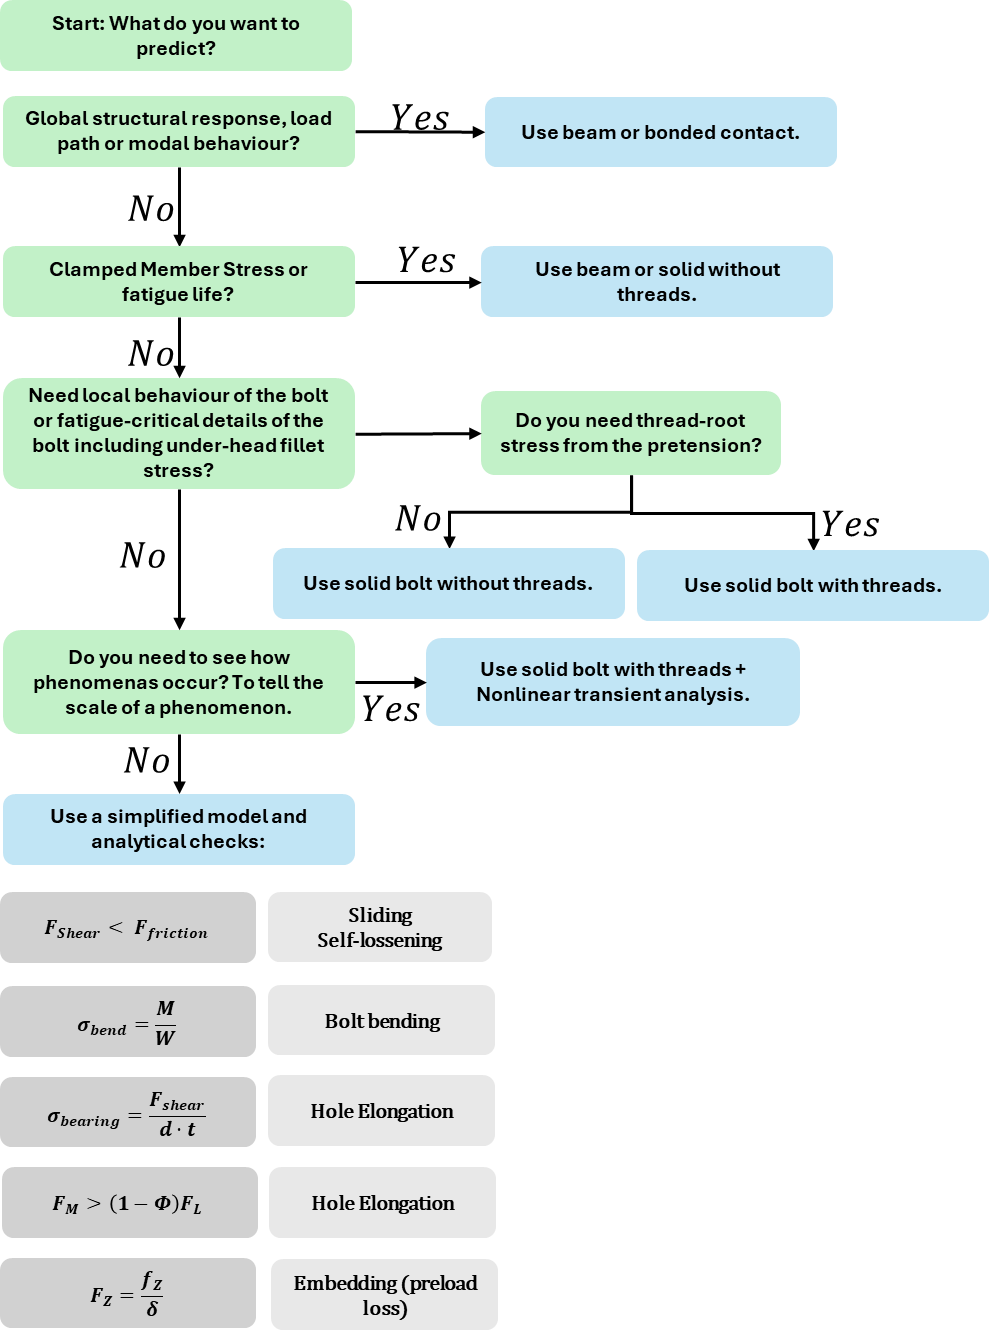
\includegraphics[width=1\linewidth]{Figures/decisionTree2.png}
    \caption{Decision flowchart for selecting a bolt FE modelling strategy. Each question is answered \emph{Yes} (the simpler model on the right is sufficient) or \emph{No} (more fidelity is required, continue down). Beam and CBUSH are capability-equivalent for global and clamped-member quantities, but the beam was the more efficient choice for the joint studied here (Section~\ref{chp:discussion}).}
    \label{fig:decisionTree}
\end{figure}


\chapter{Discussion} \label{chp:discussion}
The purpose of this thesis was to investigate how guidelines for \ac{FEA} modeling of bolted joints under random vibration can be formulated so that accuracy is balanced against computational cost. The research question was:

\begin{quote}
    \textit{\RQ}
\end{quote}

A clear pattern emerges: simplified models may be acceptable when the quantity of interest is global or located in the clamped members (not the bolt), but become inadequate when the objective is local bolt fatigue. The answer to the research question is therefore not that one universally best strategy exists among the models tested, but that the most suitable strategy depends on the response quantity of interest and where critical damage is expected. For shear random vibration loading, a beam element seems most appropriate if the engineer only needs to know the response of the clamped members. Using stiffnesses computed in accordance with VDI 2230 for a CBUSH element is inefficient, as beam elements offer greater accuracy while requiring less preprocessing time.

The main finding of this thesis is that the most suitable bolt model in \ac{FEA} depends strongly on the analysis's engineering purpose. This may seem intuitive, but the results show more specifically \textit{where} simplified models remain useful and \textit{where} they lose validity. The discussion, therefore, focuses on the relationships among physical fidelity, computational efficiency, and the type of fatigue-related question being asked.

In all cases of this thesis, the beam outperforms the CBUSH-spring element. This, however, is not always the case. According to Omar \textit{et al.}, in their work \textit{"Representation of bolted joints in a structure using finite element modeling and model updating"}, the CBUSH element connector outperforms CBEAM for representing bolted joints in modal analysis, achieving 86\% accuracy vs CBEAM of 79\% \cite{noauthor_pdf_2025}. This is not necessarily a contradiction to the results of this thesis, since the Ranking Index in this thesis is for fatigue under random vibration, and not modal analysis. They also used Swift's flexibility formula for shear stiffness, but do not state how they derived their axial stiffness, which is not a part of this thesis. They used two M10 bolts, and their stiffness does not comply with the numbers from VDI 2230, Timoshenko beam theory, and Saint-Venant, as seen in Table \ref{tab:thesisVSOmar}, where the same code that was developed for the stiffness computations in this thesis was adjusted according to their geometry:

\begin{table}[H]
    \centering
    \caption{Comparison of Stiffness - Validating the code}
    \label{tab:thesisVSOmar}
    \begin{tabular}{lrrr}
        \toprule
        Stiffness Direction & This Thesis & Omar & $100 \tfrac{(\text{Omar}-\text{VDI})}{\text{VDI}}$ \\
        \midrule
        Shear [$N/mm$]   & 246\,320.44  & 540\,300      & 119.35  \\
        Axial [$N/mm$]   & 413\,120.70  & 947\,400      & 129.33  \\
        Bending [$N\cdot mm/rad$] & 1\,812\,853.01 & 3\,458\,000\,000 & 190\,649.06 \\
        Torsion [$N\cdot mm/rad$] & 2\,848\,372.01 & 100          & -100.00  \\
        \bottomrule
    \end{tabular}
\end{table}

There is a large error in all stiffnesses, especially the bending and torsional stiffness from Timoshenko beam theory, compared to the values in Omar's work. A likely explanation for this is that they assumed the thin plates would dominate their experimental modal analysis, so they could "lock" the bending and torsional \ac{DOF}s using a penalty stiffness. This interpretation cannot be confirmed from the published information alone and should therefore be treated as a hypothesis rather than an explanation. Their value for axial stiffness is, however, very close to the simple formula $E\cdot\tfrac{A_S}{l_k} = 932\,833$ N/mm, so they probably did not divide the bolt into segments as per the frustum approach. 

\section{What the study supports}
The strongest conclusion supported by the present study is that, for the investigated bolted-joint geometry and the selected random-vibration load cases, the beam model is the best simplified alternative for predicting clamped-member fatigue-relevant response relative to the solid reference model without threads. This conclusion holds under both transverse (shear) and axial (bending) loading. It is supported consistently by the stress \ac{PSD} comparison (Figure \ref{fig:Stress_PSD_Members_Comparison}), the \ac{RMS} and fatigue life comparisons (Figure \ref{fig:RMS_per_region}, \ref{fig:Life_per_region}), and the Ranking index (Figure \ref{fig:AccuracyScore_per_region}).

Under transverse loading, the beam model achieves a clamped-members Ranking Index of 92.8, with only 4.2 \% \ac{RMS} overprediction and 84.8 \% of the solid reference life.

Under axial loading, the beam still gives the best agreement among the simplified models (Ranking Index $77.6$ for NASA and $80.9$ for T43A). It predicts $59.8 \%$ (NASA) and $69.6 \%$ (T43A) of the solid reference life, a conservative underprediction of $30-40 \%$.

The bonded model consistently overpredicts clamped-member stress by a large margin in both loading directions, yielding ranking indices of 35.4 (transverse) and 47.5 (axial). The CBUSH model performs somewhat better at 61.6 (transverse) and 45.8 (axial), but the beam remains the better option in every comparison.

All three simplified models yield conservative predictions for the clamped members. From a design perspective, this means that if a simplified model predicts acceptable fatigue life, the solid model would predict even longer life.

\section{What the study does not claim}
The results of this thesis should be interpreted within the scope defined for the study:

\begin{enumerate}
    \item The thesis does not claim that one bolt-modeling strategy is universally optimal for all bolted joints, all structures, or all vibration environments. The main conclusion is that model suitability depends on the engineering purpose, the response quantity of interest, and the dominant loading condition.
    \item The thesis does not claim absolute experimental validation of fatigue life. The reference used in this work is the highest-level numerical model considered in this thesis, but there are many more numerical fidelity levels to test. The reported Ranking index, therefore, reflects agreement with the chosen numerical reference rather than with measured fatigue failure in hardware. This is sufficient to propose a relative model ranking, but also defines a clear boundary for how far the conclusions are generalized.
    \item The thesis also does not claim validity for multiaxial random-vibration excitation, nonlinear transient contact behavior, or an assembly in which many bolts interact through load distribution. Each load case in this study was applied in one direction at a time, and the benchmark geometry was restricted to a single-bolt joint. The guidelines should therefore be understood as a decision support for comparable engineering situations, not as a substitute for detailed analysis when the joint behavior becomes strongly nonlinear.
    \item The thesis does not claim that simplified models are suitable for all local bolt assessments. The results show the opposite: simplified representations may be adequate for global response and clamped-member stress, but they fail when the engineering question concerns local bolt fatigue, under-head fillet stress, thread-root effects, or thread-related nonlinear phenomena. In those cases, higher-fidelity solid representations are required.
\end{enumerate}

\section{Interpretation of the Bolt-region findings}
In contrast to the clamped-member region, the bolt regions (underhead fillet and first engaged thread) clearly expose the limitations of the simplified models. The bonded and CBUSH models lack a discrete body, so they cannot produce meaningful stress in the bolt. The beam model does return finite stresses in all regions, but it carries the bearing load through nodal equilibrium rather than through distributed contact pressure over a real bearing surface.

Under transverse (shear) loading, the beam model overpredicts local \ac{RMS} stress by not a lot: 2.62 vs 1.90 MPa under the head and 2.69 MPa vs 1.91 MPa at the nut relative to the solid reference. In this case, the beam correctly captures the order of magnitude and even provides a conservative local life estimate.

Under axial loading, however, the behavior reverses. The solid predicts an under-head \ac{RMS} of 10.51 MPa, while the beam produces only 2.38 MPa: the beam underestimates by more than a factor of 4. The resulting beam life under the head is 1418 times the solid reference and therefore strongly non-conservative.

The same qualitative pattern appears at the nut. This happens because the axial bearing pressure under the bolt head is a distributed contact phenomenon that a single coupling node cannot represent, and is consistent with the findings of Kim \textit{et al.}, who found that simplified models match global stiffness but miss local stress \cite{27}.

The practical consequence for the guidelines is clear: when the bolt-region stress is the critical output and the dominant loading has a bending component, a 3D solid representation is required. Under shear-dominated loading, the beam can still be non-conservative locally, for instance, under NASA transverse loading, it over-predicts under-head and at-nut fatigue life by factors of 15.34 and 13.93, respectively (Table \ref{tab:fatLifeRatio}). The beam, therefore, should not be relied upon for local bolt fatigue under any bending-dominated case, and the excitation profile must qualify its use under shear loading.

\section{Loading-direction effects}
The side-by-side presentation of transverse and axial results reveals that:
\begin{itemize}
    \item The model ranking is stable in the clamped members region across loading directions. The beam model is consistently closest to the solid reference, followed by the CBUSH model and then the bonded model. This suggests that the clamped-member conclusion is robust across multiple load cases.
    \item The bolt-region behavior is direction dependent in the same way for both excitation profiles. Under transverse (shear) loading, the beam overpredicts local bolt \ac{RMS} stress (2.62 MPa vs. 1.90 MPa under-head for NASA, 0.92 MPa vs. 0.63 MPa for T43A). Under axial (bending) loading, the beam underpredicts (2.38 MPa vs. 10.51 MPa for NASA, 10.01 MPa vs. 15.13 MPa for T43A). This means that any guideline for bolt-region assessment must account for the dominant loading direction. The excitation signal does not change the over- or under-prediction in the study's case.
    \item The axial loading case produces shorter absolute fatigue lives across all models in the clamped-members region. In the bolt regions, the trend is not uniform: for the NASA case, the solid life at the nut is in fact longer under axial loading ($3.80\times10^8$ s) than under transverse loading ($4.57\times10^6$ s).
\end{itemize}

\newpage
\section{Excitation-signal effects}
As described in  Section \ref{sec:standards}, two different standardized \ac{PSD} profiles were used in this thesis: the NASA-STD-7001B Workmanship profile, which concentrates most of its energy in a relatively narrow band, and the MIL-STD-810G T43A profile, which spreads energy across a broader frequency range.

Comparing Figure \ref{fig:Life_VS_RMS_members} with Figure \ref{fig:Life_VS_RMS_members_T43A}, the Dirlik Fatigue Life in Figure \ref{fig:Life_VS_RMS_members}, with the  NASA Workmanship excitation signal, is more compliant with the expected inverse power-law relationship to \ac{RMS} stress than what is seen in Figure \ref{fig:Life_VS_RMS_members_T43A}, with the T43A signal.

Comparing Figure \ref{fig:SteinbergDirlik_members} with Figure \ref{fig:SteinbergDirlik_members_T43A}, the Dirlik and Steinberg comply more in Figure \ref{fig:SteinbergDirlik_members}, with the NASA Workmanship excitation signal, than in Figure \ref{fig:SteinbergDirlik_members_T43A}, with the T43A signal.

The interpretation is that the broadband T43A signal excites more modes simultaneously, so a mix of modal contributions with different shapes drives the stress at a given node. This widens the distribution of nodewise points around the power-law curve and reduces agreement between Dirlik (which uses a full spectral \ac{PDF}) and Steinberg (which assumes a Gaussian amplitude distribution around the RMS).

\section{SN-curve assessment with Goodman correction}

The stress state in a preloaded bolt is never fully reversed: the static preload creates a tensile mean stress $\sigma_m$ that shifts the operating point on the Haigh diagram (Figure \ref{fig:Haigh}) and shortens fatigue life. Mean stress is therefore included through the Goodman correction (Equation \ref{eq:Goodman}), which replaces the SN parameter $C$ with an effective value in accordance with Equation \ref{eq:C_eff_Goodman} and the material data $C = 4.6 \times 10^{13}$, $k = 4$, and $\sigma_u = 1040$ MPa. The correction is applied node-wise: for each node, $\sigma_m$ is extracted from the prestressed static step, and only the tensile component, $\max(\sigma_m, 0)$, is retained, since compressive mean stress does not drive fatigue crack initiation. Fatigue life is then evaluated in the frequency domain using the Dirlik formulation. For each node, the damage rate $\dot{D}$ is obtained, and the corresponding life follows from $D = \dot{D}T = 1 \rightarrow T = 1/\dot{D}$. Because the shortest-lived node governs fatigue life, the minimum life in each of the three regions of interest (clamped members, under-head fillet, and engaged threads) is used for model comparison.

The magnitude of the correction depends strongly on the region. In the clamped members, the mean stress is a small fraction of $\sigma_u$ and $C_{eff}$ is barely affected, so predicted lives are essentially unchanged. In the bolt itself, the mean stress reaches several hundred MPa from the preload, and $C_{eff}$ drops noticeably, shifting absolute lives into a more conservative region of the SN-curve. Because the same correction is applied consistently across all four bolt models, it does not change the relative ranking between them, only the absolute lives change. Further detail on the SN-curve is provided in Appendix \ref{app:SN-curve}.

The fatigue life of each simplified model is compared with the 3D threadless solid reference across four load cases (two PSDs $\times$ two directions) and three extraction regions (the clamped members, under-head fillet, and first engaged thread). Table \ref{tab:fatLifeRatio} lists the life ratios $R = \tfrac{T_{simplified}}{T_{reference}}$ for all three simplified models.

A ratio $R < 1$ means that the simplified model is conservative and predicts a shorter life span than the solid reference. A ratio $R > 1$ means that the simplified model is non-conservative and predicts longer life than the solid reference. Values close to $R = 1$ indicate agreement with the reference.

\begin{table}[H]
    \centering
    \caption{Fatigue-life ratios $R = \tfrac{T_{simplified}}{T_{reference}}$}
    \label{tab:fatLifeRatio}
    \begin{tabular}{llccc}
        \toprule
        \textbf{Load case} & \textbf{Region} & \textbf{Beam R} & \textbf{Bonded R} & \textbf{CBUSH R} \\
        \midrule
        NASA vert.  & Members    & 0.598  & 0.139  & 0.101 \\
        NASA vert.  & Under-head & 1418.6 & -    & -   \\
        NASA vert.  & At-nut     & 5.67   & -    & -   \\
        NASA horiz. & Members    & 0.848  & 0.073  & 0.264 \\
        NASA horiz. & Under-head & 15.34  & -    & -   \\
        NASA horiz. & At-nut     & 13.93  & -    & -   \\
        T43A vert.  & Members    & 0.696  & 0.0099 & 0.151 \\
        T43A vert.  & Under-head & 7.62   & -    & -   \\
        T43A vert.  & At-nut     & 1.21   & -    & -   \\
        T43A horiz. & Members    & 0.296  & 0.0259 & 0.329 \\
        T43A horiz. & Under-head & 0.202  & -    & -   \\
        T43A horiz. & At-nut     & 0.207  & -    & -   \\
        \bottomrule
    \end{tabular}
\end{table}

Three patterns can be found in the table:
\begin{enumerate}
    \item In the clamped-member region, all simplified models predict shorter fatigue life than the solid reference in all four load cases.
    \item The local bolt-region behavior of the beam model is not governed by loading direction alone. It is non-conservative for NASA transverse, NASA axial, and T43A axial loading, but conservative for T43A transverse loading.
    \item At the engaged-thread region, the beam model is non-conservative in three of the four load cases. It is conservative only for the T43A transverse case.
\end{enumerate}

These results support the use of the beam model for clamped-member fatigue in the tested benchmark. Still, they do not support a general claim that the beam is acceptable for local bolt fatigue under all shear-dominated loading. Both the excitation profile and the loading direction must be considered when qualifying the local bolt-fatigue conclusions.

\newpage
\section{Reflection on the Ranking Index} \label{sec:RIreflection}

The Ranking Index in Equation \ref{eq:AccuracyMetric} is the central decision-support contribution of the quantitative part of this thesis, and it deserves more critical reflection. The index has identifiable strengths and identifiable weaknesses.

\subsection{Strengths}
The Ranking Index has three properties that make it useful in practice. First, it includes three different response quantities (minimum Dirlik fatigue life, maximum RMS von Mises stress, and 95th-percentile RMS von Mises stress) into a single scalar that engineers can rank, plot, and communicate. Second, the construction is appropriate for the quantities involved: the fatigue-life term is taken on a logarithmic scale because fatigue lives span several orders of magnitude, and the exponatioal mapping $RI = 100e^{-E_{combined}}$ produces a smooth and intuitive 0-100 score. Third, the weighting is adjustable and its influence on the model ranking is documented in the tornado study (Figure \ref{fig:tornado}). The fact that 8 of 12 positions and three of four load cases preserve their ordering under all four weight scenarios means that the qualitative result \textit{beam - CBUSH - bonded} for clamped member fatigue is a property of the data, not of the chosen weights. Within the scope of this benchmark, the Ranking is therefore a defensible model-selection metric \textit{if} the decision is not phenomena-driven.

\subsection{Weaknesses}
At the same time, four weaknesses should be acknowledged. The first is that the weights are an engineering judgment rather than a derived quantity - there is no underlying cost or risk function that fixes 0.50/0.30/0.20 as objectively correct. They are defensible defaults for a fatigue-driven application, but they are not unique. The second is that the index measures \textit{agreement with the threadless solid reference}, not accuracy against physical measurements. The third is information loss: combining three response quantities into a single number means that two models can earn similar scores for very different reasons: one through good fatigue agreement and poor RMS agreement, the other through the opposite pattern. The fourth is that the index is symmetric in the error direction. An under-prediction of stress (overprediction of life) is treated the same as an over-prediction of equal magnitude, even though the first is the unsafe direction.

\newpage
\subsection{How the Ranking Index could be improved}
Several extensions would directly address the weaknesses and increase the usefulness of the index. 

\begin{enumerate}
    \item Asymmetric error penalty: replace the absolute-value error terms by a piecewise weighting that penalizes unsafe-side errors.
    \item Validation against physical test data: shifting the ranking index from "agreement with a slightly less simplified FE model" to something closer to "accuracy" requires a higher-fidelity reference than the threadless solid.
    \item An uncertainty term: adding a fourth term that captures the variability of the response across the critical nodes would BE BAD to models that match the reference \textit{on average}, but mispredict the location of the critical node. In this thesis, the work is done by hand, but it could just as well be built in.
    \item Better cost-function: the efficiency ratio currently combines wall-clock time and CPU time. Adding memory (RAM) and preprocessing effort would make the cost side of the index more fully reflect industrial costs, particularly for large assemblies.
\end{enumerate}

\subsection{Relevance}
As for how relevant the Ranking Index is, the honest answer is that its relevance is conditional. The index is relevant as a benchmark internal comparison tool: it gives a transparent, weight-aware, sensitivity-tested ordering of four bolt representations against a common reference under standardized excitations, and the ordering it produces is consistent with the qualitative findings from the underlying stress- and life plots. As a general-purpose accuracy metric for arbitrary bolted-joint problems, it is less relevant because the geometry, the numerical reference, the chosen weights, and the two PSDs limit its transferability. In this thesis, the phenomenon-method matrix (Table \ref{tab:phenomenaMethodMatrix}) is the more transferable deliverable: it tells an engineer \textit{which} bolt representations can, in principle, capture a given phenomenon, independent of the specific benchmark. The Ranking Index indicates to the engineer \textit{how much} the candidate representations differ on a concrete fatigue-relevant benchmark. These two deliverables are therefore complementary.

\chapter{Conclusions and Future Work} \label{chp:conclusions}

\section{Conclusions}
This thesis set out to answer the research question stated in Section \ref{sec:problemStatement} and to test the corresponding hypothesis: that practical guidelines can be formulated as a phenomenon-method matrix and a decision flowchart, driven by phenomenon, fatigue accuracy, and cost.

The results and analysis in Chapter \ref{chp:results} and the discussion in Chapter \ref{chp:discussion} support the hypothesis. It is possible to formulate practical guidelines for selecting an \ac{FEA} bolt representation for random-vibration fatigue. The guidelines take the form of two deliverables that together answer the research question: a phenomenon-method matrix (Table \ref{tab:phenomenaMethodMatrix}) that links the physical phenomenon of interest to the cheapest capable method, and a decision flowchart (Figure \ref{fig:decisionTree}) that walks the engineer from the target engineering question to a recommended model and analysis type. The efficiency ratio $\eta$ defined in Chapter \ref{chp:method} allows the user to tune the accuracy-cost trade-off.

The sub-questions (SQ) stated in Section \ref{sec:problemStatement} are answered as follows.\textit{SQ1} (which phenomena require a high-fidelity bolt representation): the phenomenon-method matrix (Table \ref{tab:phenomenaMethodMatrix}) identifies three-root SCF, stage-2 self-loosening, residual torsional bolt stress, and the full resolution of slipping as phenomena that cannot be captured below the fully-threaded solid level. Under-head fillet stress and hole elongation require at least a threadless 3D solid. \textit{SQ2} (response quantities for which simplified models are sufficient): the benchmark shows that global shear is captured by the beam and CBUSH representations, with the beam providing the closest agreement with the threadless solid reference for clamped member fatigue across the load cases studied. \textit{SQ3} (how cost and accuracy should be compared): the Ranking Index (Equation \ref{eq:AccuracyMetric}) combined with the wall-clock/CPU cost metric (Section \ref{sec:costMetric}) yields the efficiency ratio used in Chapter \ref{chp:results}, which is the workflow recommended by these guidelines.


The main findings are:

\begin{itemize}
    \item No single method is universally best.
    \item For clamped-member fatigue, the beam is the closest agreement in this specific case.
    \item For local bolt fatigue (under-head fillet, first engaged thread), a 3D solid is required. The bonded and CBUSH models cannot produce meaningful stresses in the bolt body, and the beam captures the order of magnitude under shear loading but under-predicts local stress by more than a factor of four under bending loading.
    \item Thread-level phenomena require the fully threaded solid, but simplified methods are enough to provide a binary answer as to whether the risk of phenomena exists or not.
    \item The Dirlik and Steinberg fatigue-life estimates agree closely for the narrowband NASA Workmanship excitation and agree less closely for the broadband MIL-STD-810G T43A excitation. The model-ranking conclusions, however, are robust to this choice of spectral-damage method.
    \item The Goodman mean-stress correction does not change the relative ranking of the models. It reduces the absolute fatigue life in the bolt region, where static preload stress is high, while leaving clamped-member life essentially unchanged.
\end{itemize}

This thesis supports the view that \ac{FE} model selection for bolted joints under random vibration should depend on the physical phenomena of interest and the required response quantity. This is supported by two different forms of evidence: a phenomenon-method matrix and a computational experiment. The thesis does not claim experimental or universal validation of the full matrix. Instead, it provides a scoped aid for engineering judgment, combining literature-based capability mapping with benchmark-based evidence on accuracy and computational cost. The hypothesis is supported within the stated scope of the thesis.

\section{Contributions}

This thesis presents three deliverables for engineers conducting finite-element analysis of bolted joints subjected to random vibration fatigue. These are the contributions:

\begin{enumerate}
    \item A phenomenon-method matrix (Table \ref{tab:phenomenaMethodMatrix}) linking eight physical phenomena that bolted joints may experience under random vibration to the cheapest \ac{FE} representation capable of capturing each.
    \item A decision flowchart (Figure \ref{fig:decisionTree}) that walks an engineer from the engineering question to a recommended model type and analysis setup.
    \item A quantitative accuracy-cost comparison between four bolt-model fidelities that, through the Ranking Index and the Cost function, combines fatigue-life accuracy, \ac{RMS} stress accuracy, and computational cost into a single scalar.
\end{enumerate}

The literature review in Chapter \ref{chp:relatedwork} shows that important parts of the problem are already well covered individually. Spectral fatigue methods are well established, bolt model fidelity has been studied in static and modal contexts, and nonlinear joint dynamics have been investigated experimentally. What is missing in the literature is a single framework that connects this information for the specific purpose of model selection under random-vibration fatigue. This thesis contributes to reducing that gap in the following ways:
\newpage
\begin{enumerate}
    \item Kim \textit{et al.} compared four bolt representations (solid, coupled, spider, no-bolt) under static loading and modal analysis, and showed that simplified models can reproduce global behavior at reduced cost \cite{27}. Omar \textit{et al.} extended similar comparisons to modal analysis with model updating, reporting that CBUSH connectors outperformed CBEAM for the joints they studied \cite{noauthor_pdf_2025}. Naruse \textit{et al.} compared solids and beam elements against VDI 2230 predictions of equivalent stiffness \cite{09}. None of these studies extends the comparison to frequency-domain fatigue under a standardized \ac{PSD} excitation. This thesis adds that missing part: four bolt FE-representations are benchmarked under NASA-STD-7001B and MIL-810G excitations across two loading directions, with Dirlik fatigue life and \ac{RMS} von Mises stress as the response quantities of interest (Chapter \ref{chp:results}, Tables \ref{tab:MinLife} and \ref{tab:MinLifeVtical}).
    \item The works above report which model was best in their specific test case. They do not state which physical phenomena each simplification can or cannot represent. Engineers facing a new joint configuration, therefore, lack a basis for choosing a model before running any simulation. The phenomenon-method matrix (Table \ref{tab:phenomenaMethodMatrix}) constructed in this thesis reduces that gap by listing eight physical phenomena relevant to bolted joints under random vibration and maps each to the cheapest \ac{FE} representation that can still capture it at a useful engineering level. The associated decision flowchart (Figure \ref{fig:decisionTree}) outlines a workflow for an engineer to follow before building a model.
    \item Segalman \textit{et al.} provided an efficient method for computing \ac{RMS} von Mises stress in a random-vibration environment \cite{segalman_efficient_2000}. Halfpenny reviews frequency-domain fatigue analysis from PSDs and reports that the Dirlik method gives good agreement with time-domain fatigue estimates in the studied cases \cite{halfpenny_frequency_1999}. Dirlik and Steinberg established different frequency-domain damage estimations from stress PSDs \cite{dirlik_application_1985}. These methods are used, but by themselves do not indicate which \ac{FE} bolt representation is appropriate for use with their algorithms. This thesis introduces a Ranking Index (Equation \ref{eq:AccuracyMetric}) and a Cost metric (Table \ref{tab:WC_CPU}) that, together, yield a single Efficiency Ratio for each model, region, and load case. The Ranking Index combines log-scale fatigue-life error and two RMS-stress errors into a single scalar, enabling the output of Segalman-based analysis to be consistently compared across model fidelities.
\end{enumerate}

Taken together, these contributions move the problem from “which model is best?” to the more useful and more general engineering question: “which model is adequate for this specific purpose at the lowest justified cost?”
\newpage
\section{Future work}
The present work can be extended in several different directions. Below are some of these, motivated by scoping decisions made in the present work:

\begin{enumerate}
    \item Experimental validation: the reference model used here is a 3D threadless solid, not a physical test. A vibration test of the geometry on a shaker table, instrumented with strain gauges at the critical regions, would convert the Ranking Index from a relative score against a higher fidelity numerical model into a score relative to a measurement.
    \item Multi-bolt patterns: the single-bolt benchmark used here cannot capture load-sharing redistribution between fasteners. Repeating the same four-model comparison on a representative multi-bolt geometry would test whether the model ranking established for the single-bolt geometry is preserved.
    \item Alternative bolt representations: the four models used in this work are not the only representations available. For example, Kim \textit{et al.} modeled a bolt with a solid head and nut, but having the shank only represented by a beam \cite{27}. Another model, which is less available in commercial software but can be implemented as a custom element, is the reduced Iwan model, as described by Brake \textit{et al.} \cite{brake_reduced_2017}. That model represents the system as a set of springs and friction elements with a defined set of degrees of freedom.
    \item Material sensitivity: All simulations in this thesis used isotropic linear elastic properties for structural steel ($E=200$ GPa, $\nu = 0.30$). Two other material classes commonly used in the application are aluminum alloys with $E\approx 70$ GPa, $\nu \approx 0.33$, and titanium with $E\approx116$ GPa, $\nu = 0.32$.
    \item Multi-axial excitation: the present work applies excitation in one direction at a time. Repeating the benchmark with PSDs simultaneously applied across multiple axes would close this scoping gap and clarify whether the ranking holds under realistic test conditions.
    \item Nonlinear transient analysis: extending the comparison to fully nonlinear transient analysis with the threaded solid representation would allow other phenomena to influence fatigue life in the benchmark. It would also test the central assumption that contact states can be frozen at the prestressed state.
    \item More phenomena: the eight phenomena that are assessed in the present work are not all phenomena. Identifying additional fatigue-driving phenomena and their analysis requirements would further reduce the research gap.
    \item Asymmetric Ranking Index against a physical test reference: redefine the error terms with a higher penalty on the unsafe side (life over-prediction, stress under-prediction) and replace the \ac{FE} reference with vibration-fatigue test data. This would shift the index from a measure of model agreement to one of model accuracy, making it more usable as a design-decision metric. Other improvements of the Ranking Index are identified in Section \ref{sec:RIreflection} and can be added on top of this redefinition.
\end{enumerate}


% All references are in a separate file: thesis-refs.bib
\bibliography{references}
\bibliographystyle{plain}


\appendix

\chapter{Mesh Convergence} \label{app:MeshConvergence}

From the SN-curve, the relationship $N=S^{-k}$ shows that for an error $\epsilon$ at the stress, it becomes $N_e=(S+\epsilon)^{-k} = \epsilon^{-k}S^{-k}$. This means that $\tfrac{N_e}{N} = \epsilon^{-k}$. If the error is, for example, a 10 \% overprediction in stress, with $k=4$ for steel, the cycles get an error of

\begin{equation}
    N=(1.1S)^{-4} = 1.1^{-4}S^{-4} = 0.68S^{-4}.
\end{equation}
That is an error of 32 \% lower life. If the error is a 10\% underprediction in stress, in the same material, the cycles get an error of

\begin{equation} \label{eq:underEstimateStress}
    N=(0.9S)^{-4} = 0.9^{-4}S^{-4} = 1.52S^{-4},
\end{equation}

which corresponds to 52 \% higher predicted life. This means that convergence tolerances must be tighter for this type of analysis than for a static analysis.

In the work of this thesis, the convergence criteria are:
\begin{itemize}
    \item Modal frequencies: $\pm 1 \%$ on the first 10 modes.
    \item Peak stress \ac{PSD} values at critical nodes: $\pm 5 \%$.
    \item Minimum Dirlik fatigue life: $15\%$.
\end{itemize}

Figure \ref{fig:ModeFreqsConv} shows the convergence of the first ten natural frequencies with increasing mesh density. The modal frequencies are essentially stable across all densities (Figure \ref{fig:ModeFreqsConv}), and all reported modes satisfy the $1 \%$ convergence criterion. The largest difference occurs for Mode 6, which is at the tolerance limit, while all other modes are below the limit. This indicates that the global dynamic stiffness has been sufficiently determined for the frequency-response analysis. 

\begin{figure}[H]
    \centering
    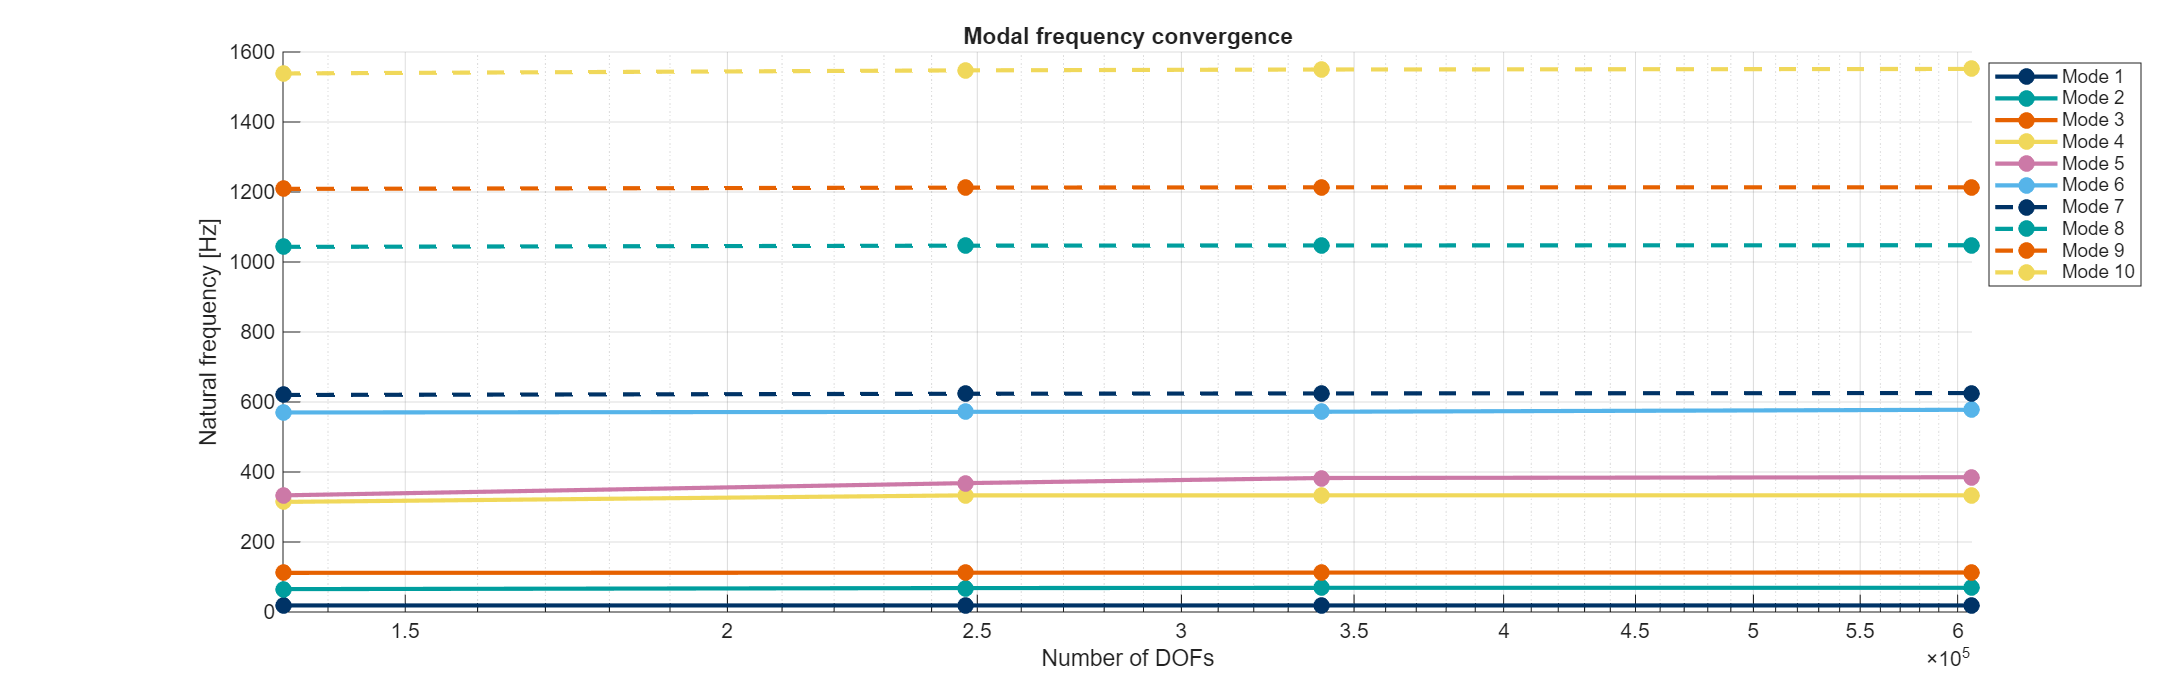
\includegraphics[width=1\linewidth]{convergence_plots/modal_frequency_convergence.png}
    \caption{Modal Frequencies for four mesh refinements}
    \label{fig:ModeFreqsConv}
\end{figure}

Note that these mode frequencies are for the fixed-free condition that is used in the fatigue analysis, not the cross-validation to the free-free experiment performed by Kim \textit{et al.}, which is done in Figure \ref{fig:modal27} in Section \ref{sec:validity}.

For the clamped-member region, the convergence behavior is shown in Figure \ref{fig:MemberConv}. The coarse mesh gives the highest \ac{RMS} stress levels, while the medium mesh already captures the trend. The fine and finer meshed lie close to each other, indicating that the local stress in the members has stabilized. Between the fine and finer meshes, the relative difference is 1.82 \% for the maximum \ac{RMS} stress and 1.59 \% for the average \ac{RMS} stress, both of which are below the 5\% limit.

\begin{figure}[H]
    \centering
    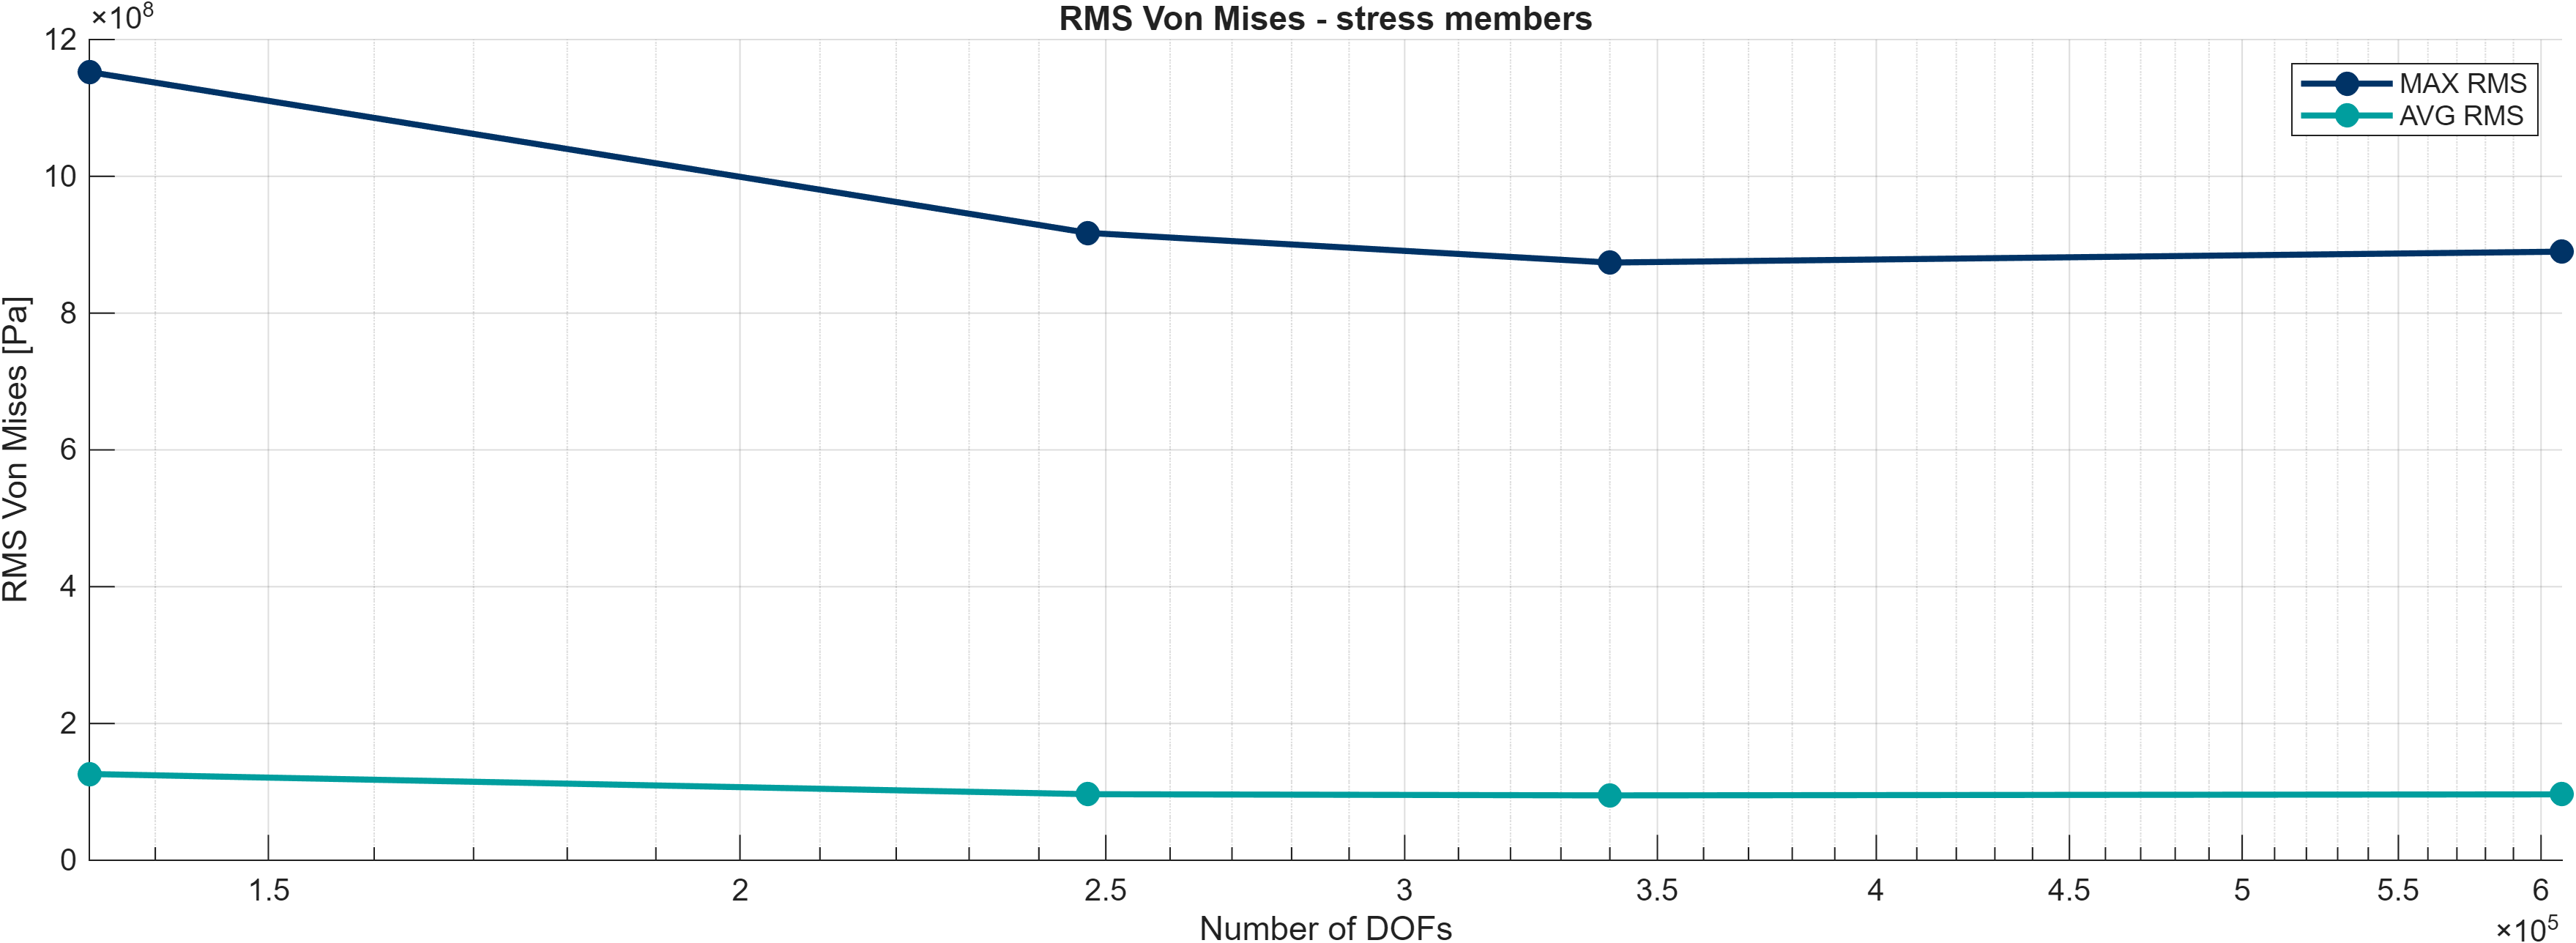
\includegraphics[width=0.75\linewidth]{convergence_plots/rms_von_mises_absolute_stress_members.png}
    \caption{Equivalent stress convergence at the clamped members for four mesh refinements.}
    \label{fig:MemberConv}
\end{figure}

The same conclusion is in the spectral comparison. The equivalent stress \ac{PSD} at the worst node shows that the coarse mesh shifts the dominant high-frequency peak to different frequencies, whereas the fine and finer meshes are nearly identical. This indicates that the fatigue spectra have converged, as seen in Figure \ref{fig:segalmanConv}.

\begin{figure}[H]
    \centering
    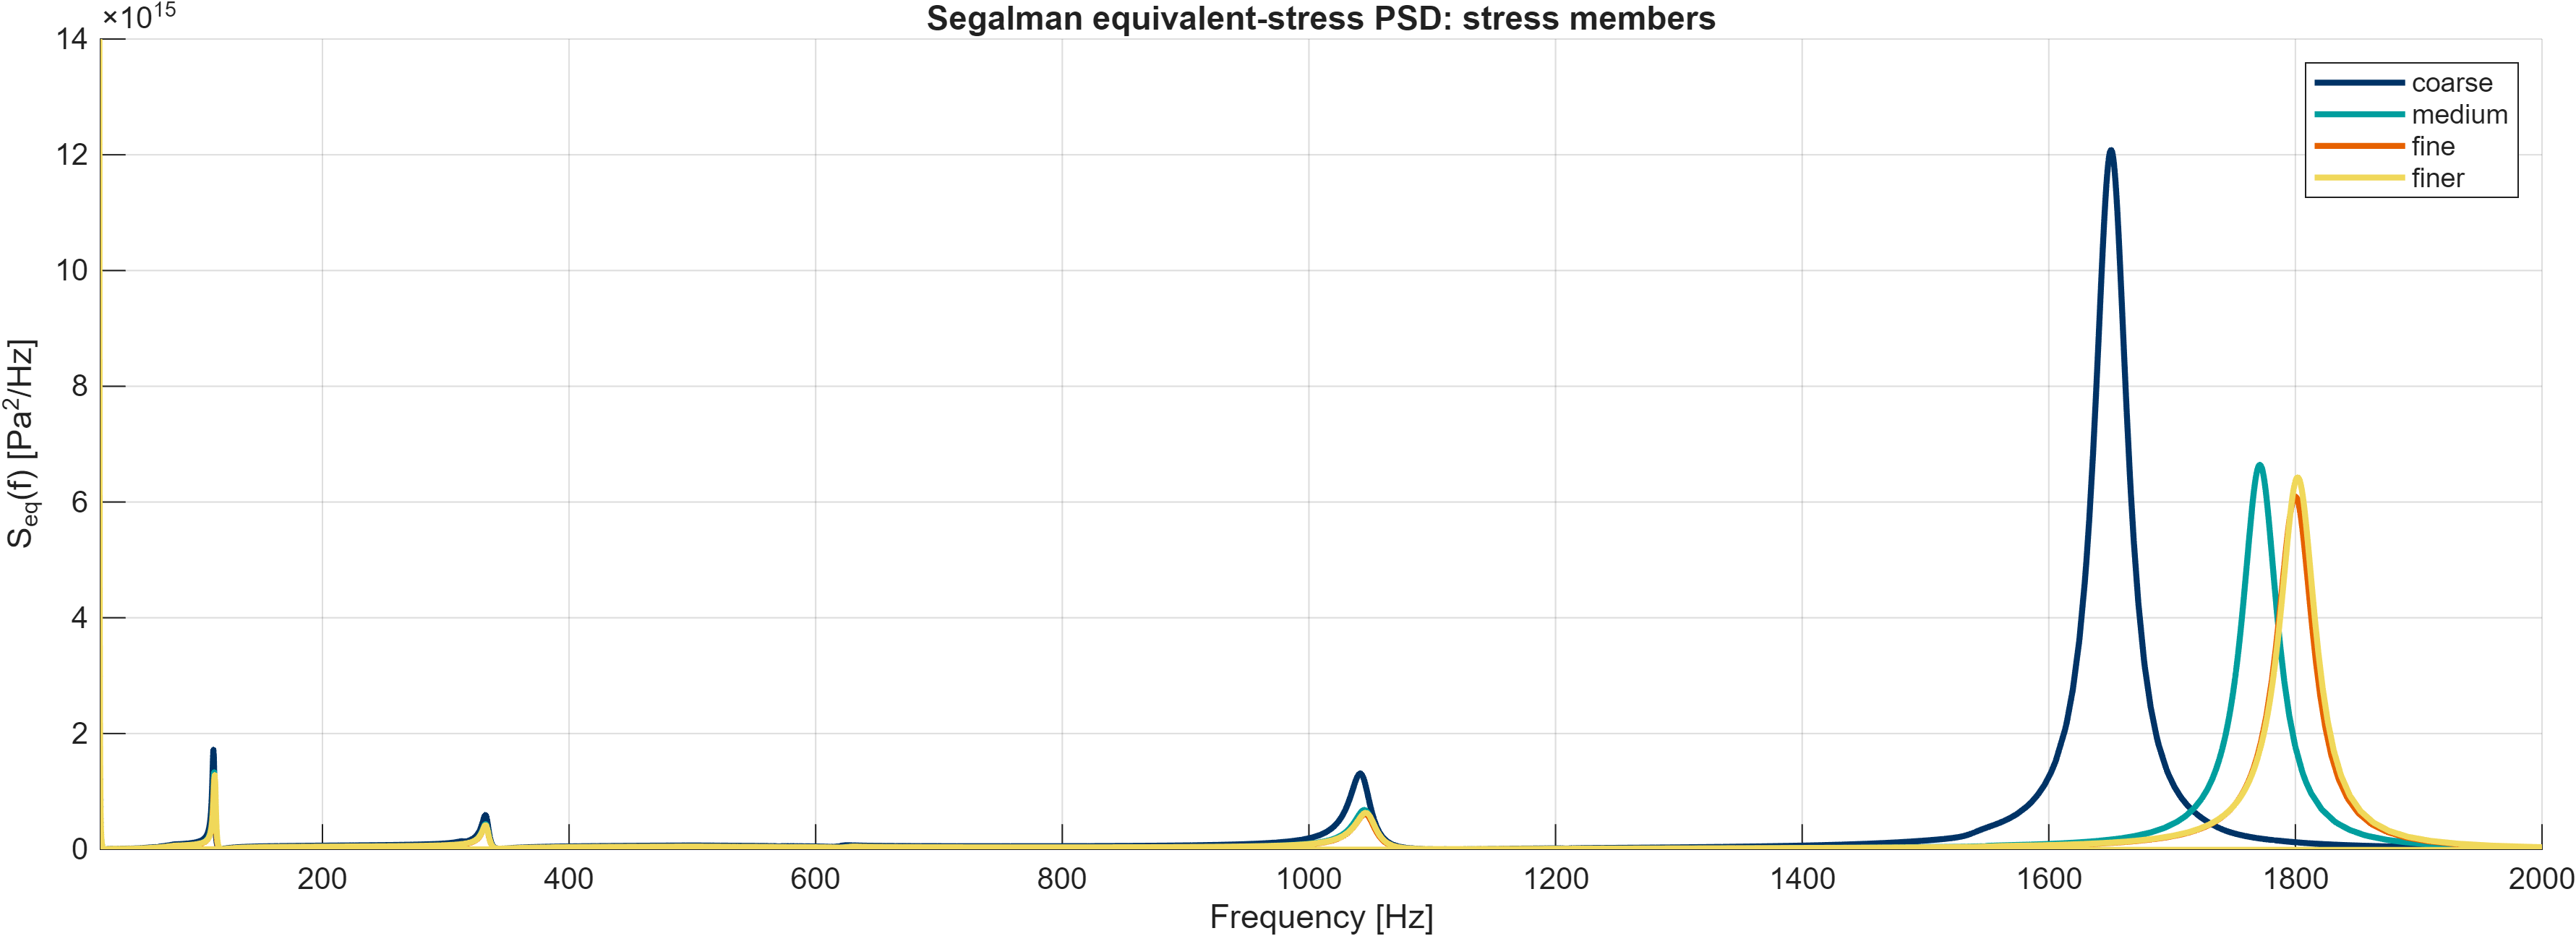
\includegraphics[width=1\linewidth]{convergence_plots/worst_node_stress_psd_stress_members.png}
    \caption{Convergence of Segalman stress spectra for four mesh refinements.}
    \label{fig:segalmanConv}
\end{figure}


The fatigue-life metrics also meet the convergence targets. The relative difference between the fine and finer meshes is 2.83 \% for the Dirlik \ac{RMS} stress and 10.51 \% for the minimum Dirlik life, both within the limits, as seen in Figure \ref{fig:FLConv}. The mesh is therefore considered converged for the fatigue assessment.

\begin{figure}[H]
    \centering
    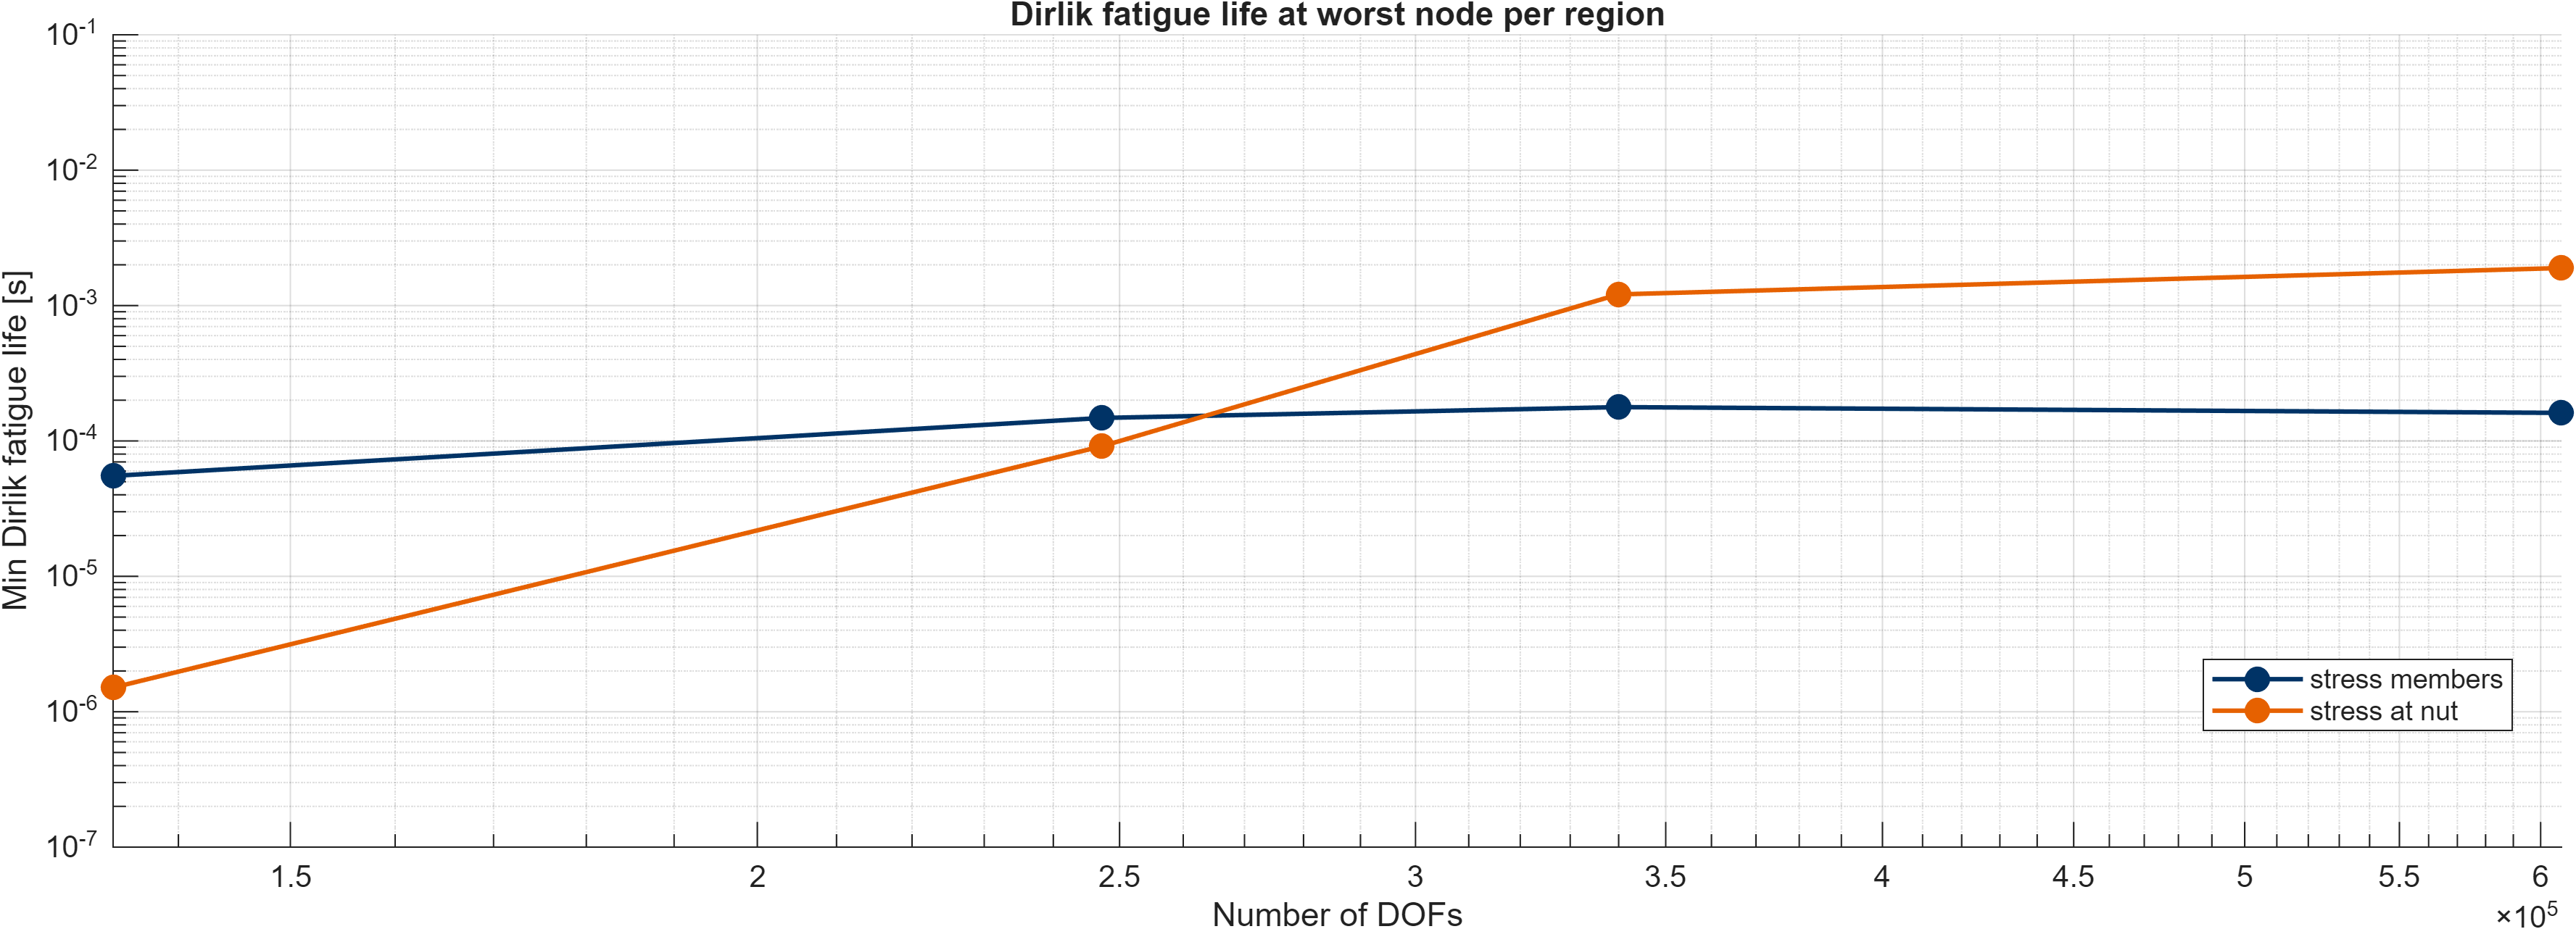
\includegraphics[width=1\linewidth]{convergence_plots/dirlik_fatigue_life_absolute.png}
    \caption{Fatigue Life convergence}
    \label{fig:FLConv}
\end{figure}

The assembly is discretized with a three-dimensional solid mesh of eight-node hexahedral elements (CHEXA), which account for 99.97\% of the solid elements in the model. The remaining 0.03\% are six-node penntahedral elements (CPENTA) used only as wedge-fillers in the few transition regions where a structured hexahedral mesh cannot be maintained. The same element type is used across every solid component of the joint (bolt, nut, washer, and clamped plates), which keeps the contact interfaces, the pretension load path, and the stress field in the bolt regions on a consistent discretisation.

Hexahedral elements are preferred here because, at a given element size, they exhibit lower volumetric and shear locking than tetrahedral elements and resolve the steep stress gradients near the under-head fillet and the first engaged thread more accurately for the same number of \ac{DOF}s \cite{tadepalli_comparison_2011}. Given the negligible pentahedral fraction, the mesh can be treated as fully hexahedral for the purposes of the comparison in Chapter \ref{chp:results}.


\chapter{Ranking Index Results} \label{app:RI_tables}

\begin{table}[H]
    \centering
    \caption{Ranking Index Transverse NASA}
    \label{tab:RI_table_VerticalNasa}
    \begin{tabular}{lrrrrr}
        \toprule
        \textbf{Model}  & \textbf{$E_{life}$} & \textbf{$E_{max\, RMS}$} & \textbf{$E_{95\, RMS}$} & \textbf{$E_{combined}$} & \textbf{RI} \\
        \midrule
        Solid  & 0.000 & 0.000 & 0.000 & 0.000 & 100.0 \\
        Beam  & 0.223 & 0.133 & 0.512 & 0.254 & 77.6 \\
        Bonded  & 0.856 & 0.611 & 0.667 & 0.745 & 47.5 \\
        CBUSH  & 0.995 & 0.759 & 0.276 & 0.780 & 45.8 \\
        \bottomrule
    \end{tabular}
\end{table}

\begin{table}[H]
    \centering
    \caption{Ranking Index Transverse NASA}
    \label{tab:RI_table_HorizontalNasa}
    \begin{tabular}{lrrrrr}
        \toprule
        \textbf{Model}  & \textbf{$E_{life}$} & \textbf{$E_{max\, RMS}$} & \textbf{$E_{95\, RMS}$} & \textbf{$E_{combined}$} & \textbf{RI} \\
        \midrule
        Solid  & 0.000 & 0.000 & 0.000 & 0.000 & 100.0 \\
        Beam  & 0.072 & 0.042 & 0.133 & 0.075 & 92.8 \\
        Bonded  & 1.139 & 0.909 & 0.988 & 1.040 & 35.4 \\
        CBUSH  & 0.579 & 0.401 & 0.372 & 0.484 & 61.6 \\
        \bottomrule
    \end{tabular}
\end{table}

\begin{table}[H]
    \centering
    \caption{Ranking Index Transverse T43A}
    \label{tab:RI_table_VerticalT43A}
    \begin{tabular}{lrrrrr}
        \toprule
        \textbf{Model}  & \textbf{$E_{life}$} & \textbf{$E_{max\, RMS}$} & \textbf{$E_{95\, RMS}$} & \textbf{$E_{combined}$} & \textbf{RI} \\
        \midrule
        Solid  & 0.000 & 0.000 & 0.000 & 0.000 & 100.0 \\
        Beam  & 0.157 & 0.090 & 0.530 & 0.212 & 80.9 \\
        Bonded  & 2.007 & 2.890 & 2.797 & 2.430 & 8.8 \\
        CBUSH  & 0.821 & 0.582 & 0.150 & 0.615 & 54.1 \\
        \bottomrule
    \end{tabular}
\end{table}

\begin{table}[H]
    \centering
    \caption{Ranking Index Transverse T43A}
    \label{tab:RI_table_HorizontalT43A}
    \begin{tabular}{lrrrrr}
        \toprule
        \textbf{Model}  & \textbf{$E_{life}$} & \textbf{$E_{max\, RMS}$} & \textbf{$E_{95\, RMS}$} & \textbf{$E_{combined}$} & \textbf{RI} \\
        \midrule
        Solid  & 0.000 & 0.000 & 0.000 & 0.000 & 100.0 \\
        Beam  & 0.528 & 0.353 & 0.198 & 0.410 & 66.4 \\
        Bonded  & 1.587 & 1.779 & 1.188 & 1.565 & 20.9 \\
        CBUSH  & 0.483 & 0.346 & 0.346 & 0.415 & 66.1 \\
        \bottomrule
    \end{tabular}
\end{table}


\chapter{Bolt Derivations} \label{app:bolt_derivations}

\section{VDI 2230 bolt theory} \label{sec:VDIApp}
The VDI 2230 standard \textit{"Systematic calculation of high duty bolted joints Joints with one cylindrical bolt"} is an analytical framework for bolted joint design published by the Association of German Engineers (Verein Deutscher Ingenieure, VDI). It computes several important metrics and phenomena, including stiffness, strength, and fatigue resistance. 

\subsection{Distribution of Applied Torque}
When torque is applied to a threaded fastener, not all of the energy is converted into useful work. Instead, the applied torque is distributed across three main areas, with only a small fraction contributing to the desired bolt tension. According to Shoberg's VDI 2230 review, approximately 50 \% or more of the applied torque is absorbed by friction at the bearing surface \cite{VDI_Fundamentals}. He states that an additional 40 \% is typically absorbed by friction between the threads. Only the remaining 10 \% of the applied torque contributes usefully to the stretching of the bolt and compressing of clamped components.

\subsection{The equivalent Cone Model for Joint Compliance}
In reality, the stress that the bolt joint causes in the clamped members does not extend infinitely outward from the bolt hole. The stress spreads and forms an angle, forming a region with a shape similar to a truncated cone (a frustum) of significant compression.

The cone model in the VDI 2230 is described by its angle $\varphi$, using Equation 5.1/27 in the VDI 2230 that takes the ratio $\beta_L$ of the grip length $l_k$ to the outer diameter of the head-bearing surface $d_w$ and the ratio $y$ of the outer diameter of the substitution cylinder $D_A'$ to the bearing diameter $d_w$ \cite{VDI} into account. The angle $\varphi$ is not the geometric angle of the compression (stress) cone, it's a curve-fitting parameter used solely to compute the correct joint stiffness \cite[p.35]{VDI}. The equation to compute $\varphi$ is given by Equation \ref{eq:tanPhi}:

\begin{equation} \label{eq:tanPhi}
    \tan({\varphi}) = 0.362 + 0.032 \times \ln\left(\frac{\beta_L}{2}\right) + 0.153 \times \ln\left(y\right)
\end{equation}

With
\begin{equation}
    \beta_L = \frac{l_k}{d_w}
\end{equation} and
\begin{equation}
    y = \frac{D_A'}{d_w}
\end{equation}

The cone angle (not $\varphi$) determines how steeply this stress spreads. A small angle implies that the stress remains concentrated near the bolt hole (stiff joint). A large angle means the stress spreads more broadly into the surrounding material (a more compliant joint). 

The substitutional outside diameter $D_A$ represents the effective width of the compressed material. The standard "converts" different geometries into a simple equivalent cylinder with diameter $D_A$ to enable the calculation.

The question is \textit{"Does the geometry constrain the cone?"}

If yes, that is, the cone "wants" to go further than the geometry can permit due to a too small distance from the hole to the geometry boundary. The entire part acts as a deformation body, and $D_C$ equals the smallest distance from the hole center to the geometry end, multiplied by 2.

If not (if the cone is allowed to extend freely without penetrating the geometry), the pressure is limited only by the angle of the pressure cone. $D_C$ is then defined as the diameter of the pressure cone at the interface between the clamped parts \cite{VDI}. Since this yields a pressure function dependent on pressure, the diameter is calculated iteratively using equation \ref{eq:tanPhi} together with the following Equation \ref{eq:D_A}:

\begin{equation} \label{eq:D_A}
    D_A \approx d_w + w\times l_k \tan(\varphi)
\end{equation}

For a through-bolted joint, $w$ is equal to one, and for a tapped-thread joint, $w$ is equal to two. By first using equation \ref{eq:D_A} with the maximum $tan(\varphi)$ that it can have (1), and comparing it to the smallest distance from the bolt to the end of the geometry (the maximum cone width), we can determine which definition is valid \cite{VDI}.

A limiting diameter $D_{A, Gr}$ separates three cases, in the VDI 2230:

\begin{equation} \label{eq:D_AGR}
    D_{A, Gr} = d_w + w\times l_k \tan(\varphi)
\end{equation}

\begin{itemize}
    \item If ($D_A \ge D_{A, Gr}$), then the cone can spread freely and the stress is distributed as "Pure cone". The clamped parts' compliance is calculated by Equation \ref{eq:delta_P1}
    \begin{equation} \label{eq:delta_P1}
        \delta_P = \frac{ 2 ln\left( \frac{(d_w+d_h)(d_w + w l_k tan(\varphi)-d_h)}{(d_w-d_h)(d_w - w l_k tan(\varphi)+d_h)}\right)}{w E_p \pi d_h tan(\varphi)}
    \end{equation}
    \item Else If ($d_w < d_A < D_{A, Gr}$), then the cone reaches the geometry boundary, and the stress is distributed as "Cone and sleeve". The compliance combines a cone portion and a cylindrical sleeve portion:
    \begin{equation} \label{eq:delta_P2}
    \begin{aligned}
        \delta_P = \frac{1}{E_P \cdot \pi} & \Bigg[ \frac{2}{w \cdot d_h \cdot \tan\varphi} \cdot \ln \left(\frac{(d_w + d_h)(D_A - d_h)}{(d_w - d_h)(D_A + d_h)}\right) + \\
                                           &      + \frac{4}{D_A^2 - d_h^2}\left(l_k - \frac{D_A - d_w}{w \cdot \tan\varphi}\right) \Bigg]
    \end{aligned}
    \end{equation}
    \item Else If ($d_w \ge D_A$), then the bearing diameter exceeds the available joint diameter and only a cylindrical sleeve is used:
    \begin{equation} \label{eq:delta_P3}
        \delta_P = \frac{4l_k}{E_P \pi (D_A^2 - d_h^2)}
    \end{equation}
\end{itemize}

If the first condition is true, then Equation \ref{eq:delta_P1} is valid. The condition is visualized in Figure \ref{fig:Bolt Diameters}.

\begin{figure}[H]
    \centering
    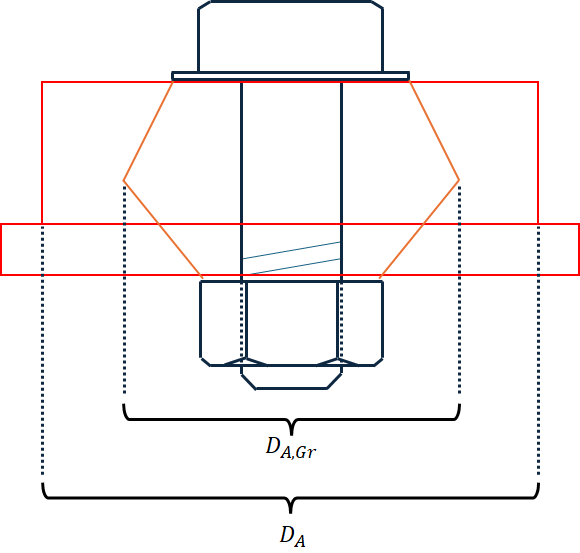
\includegraphics[width=0.5\linewidth]{Figures/Bolt Diameters.png}
    \caption{Bolt Diameters}
    \label{fig:Bolt Diameters}
\end{figure}

% Idea: pseudo code

The angle $\varphi$ is not always computed. According to the review \textit{Examining the Effects on a Fatigue Life of Preloaded Bolts in Flange Joints: An Overview} by Okorn \textit{et al.}, the angle $\varphi_D$ is approximately $30^\circ$ \cite{30}, which might be a valid approximation in some cases. The stress cone is visualized in Figure \ref{fig:coneStress}:

\begin{figure}[H]
    \centering
    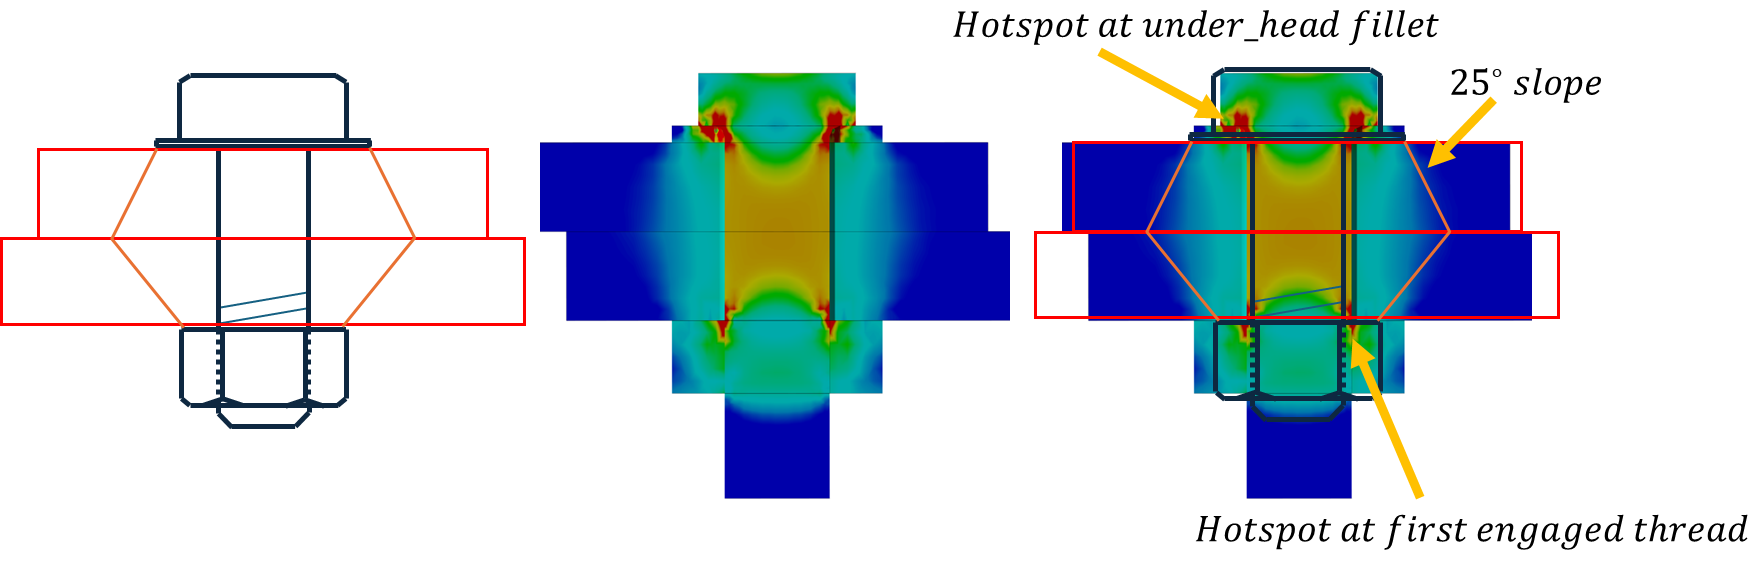
\includegraphics[width=1\linewidth]{Figures/coneStress2.png}
    \caption{The distributed stress cone}
    \label{fig:coneStress}
\end{figure}

The VDI 2230 standard treats bolted joints as systems of springs acting in series or in parallel. When a bolt is tightened, it stretches like a spring with stiffness $k_S$ (bolt stiffness), while the clamped components compress with their own stiffness $k_m$ (component stiffness). These two springs determine not only the preload, which then also affects the joint's response to external loads during service.

The bolt stiffness can be calculated using basic principles of strength of materials. To accurately compute the bolt stiffness, it is divided into sections with different properties \cite{VDI}.

\begin{figure}[H]
    \centering
    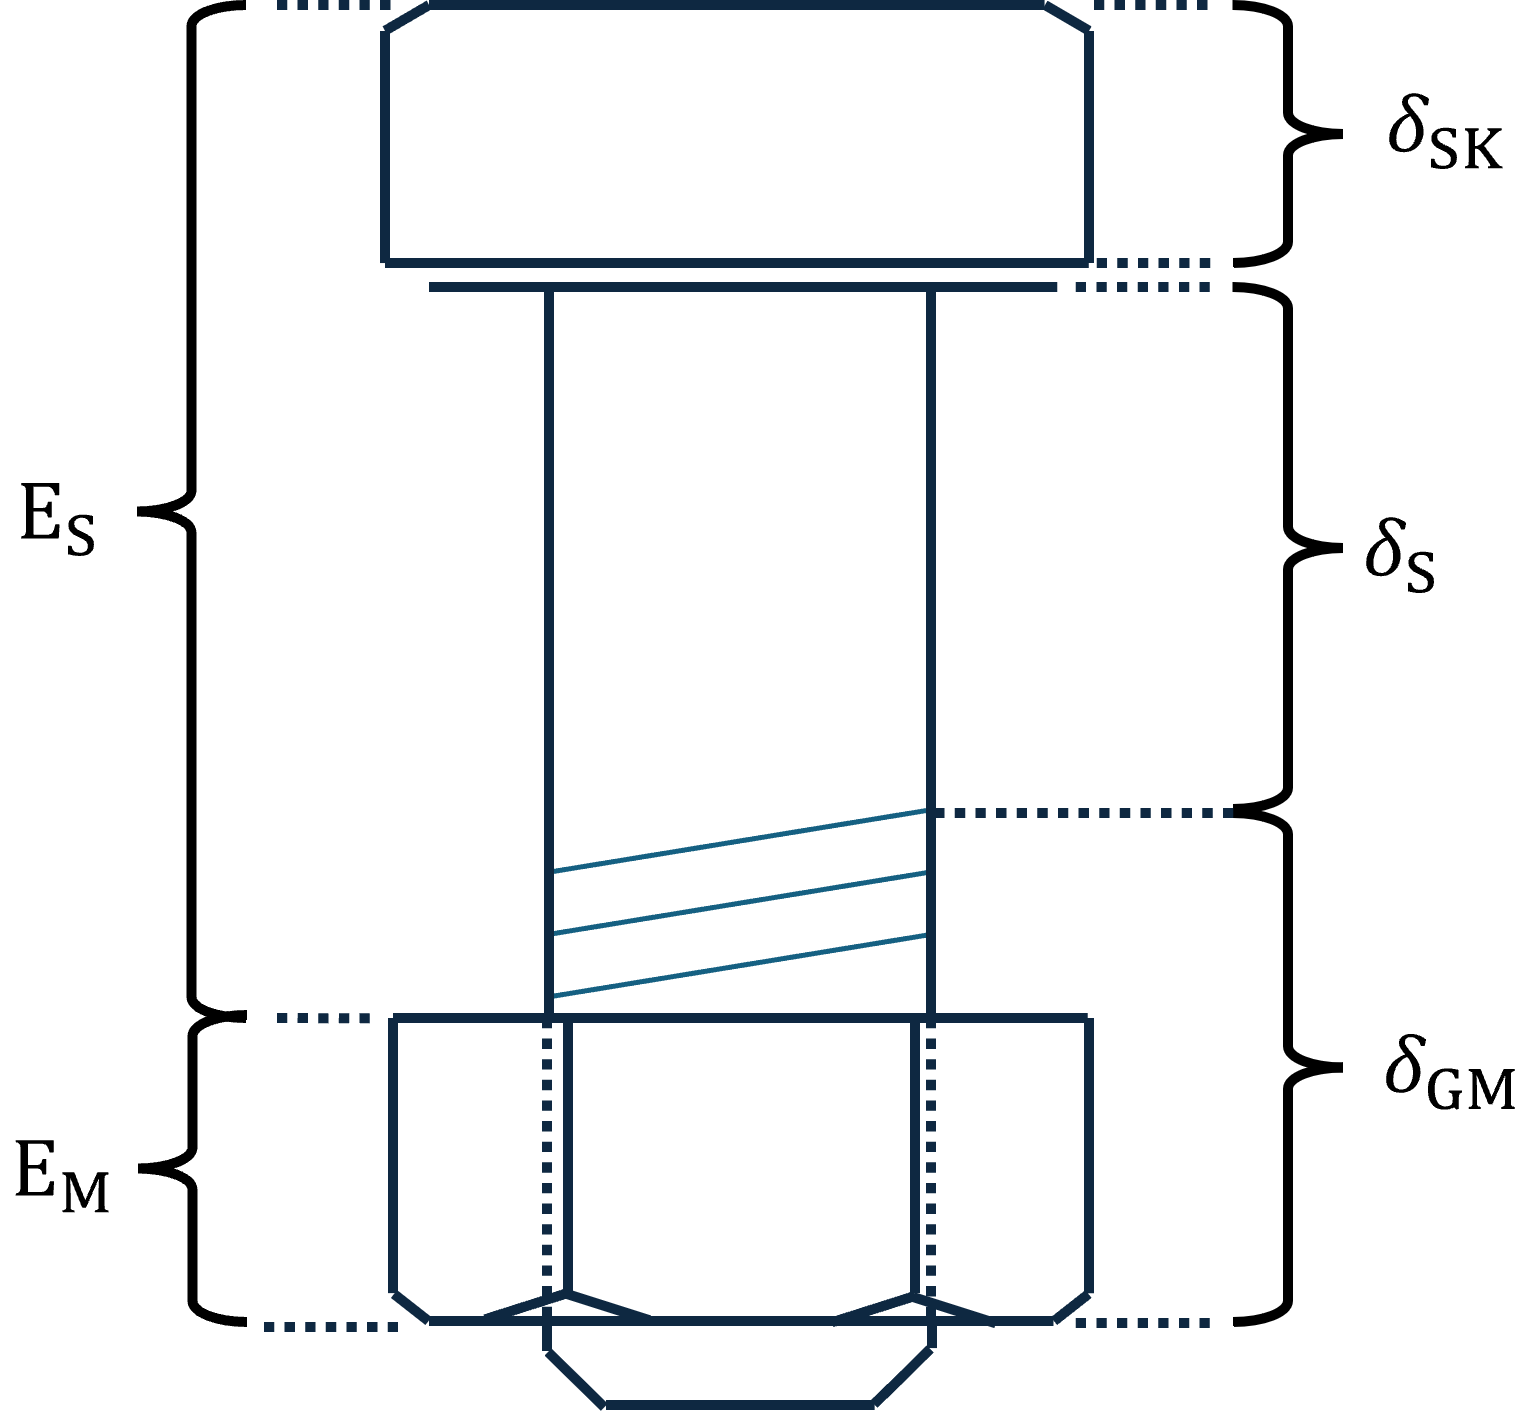
\includegraphics[width=0.5\linewidth]{Figures/Bolt_Sections.png}
    \caption{Material Property sections of bolt with nut.}
    \label{fig:Bolt_Nut_Young_compl}
\end{figure}

The different compliancies (inverse of stiffness, $\tfrac{1}{k}$) are seen to the right of Figure \ref{fig:Bolt_Nut_Young_compl}, and the Young's modulus sections of the bolts to the left, in accordance with the VDI 2230. The bolt has four distinct "sub-compliancies" that, together, form the actual compliance.

For each section $i$ of the bolt, Equation \ref{eq:delta_i} is computed and summed to the total compliance that is Equation \ref{eq:delta_sum}.

\begin{equation} \label{eq:Ai}
    A_i = \frac{\pi}{4}d_i^2
\end{equation}
\begin{equation} \label{eq:delta_i}
    \delta_i = \frac{L_i}{E_iA_i} = \frac{4 L_i}{\pi E_i d_i^2}
\end{equation}

\begin{equation} \label{eq:delta_sum}
    \delta_S = \sum_i \delta_i = \frac{4}{\pi}\sum_i\frac{L_i}{E_i d_i^2}
\end{equation}

To get the bolt stiffness, this value is inverted:
\begin{equation} \label{eq:kS}
    k_S = \delta_S^{-1} = \frac{\pi}{4 \sum_i\frac{L_i}{E_i d_i^2}}
\end{equation}

\section{Q-factor} \label{app:QFactor}
The simplest Sandia method assumes that the stress field is distributed as a cylinder of diameter $D_c$. A factor $q_i$ is defined as the ratio between the hole diameter $d_h$ and the bolt diameter $d$, taking clearance into account (Figure \ref{fig:QFactorDimensions}). The factor $Q$ can be defined in different ways:

\begin{equation}
    q_i = \frac{d_{h, i}}{d}
\end{equation}
The simplest definition of $Q$ is as the ratio between the cylinder diameter $D_A$ and the bolt diameter $d$.
\begin{equation}
    Q = \frac{D_A}{d}
\end{equation}

The guideline does, however, discuss the use of the Bickford approach, which is another way of computing the area and therefore also $Q$:

\begin{itemize}
    \item If the bearing diameter $d_w$ is larger or equal to the joint diameter $D_A$, then
    \begin{equation}
        Q = \frac{D_A}{d}
    \end{equation}
    \item If $D_A \le 3\cdot d_h$ and $l \le dh$
    \begin{equation}
        Q = \sqrt{ (d_h/d)^2 - 1 + [(D_A/d_h)^2 \cdot (1 + l_k/(10d_h)]^2 / 200 }
    \end{equation}
    \item If $D_A > 3\cdot d_h$ and $l \le dh$
    \begin{equation}
        Q = (1/d) * \sqrt{ dh^2 + (l_k/10)^2 \cdot 8 }
    \end{equation}
    \item else
    \begin{equation}
        Q_{Bickford} = (1/db) * \sqrt{ dh^2 + (min(l, dh)/10)^2 * 8 }
    \end{equation}
    \begin{equation}
        Q = max(Q_{bickford}, dh/d)
    \end{equation}
\end{itemize}

Just as for the VDI 2230, the bolt is divided into different sections, and the axial compliance of the bolt itself is computed in the same way. The difference lies in how the area of each section $A_i$ is calculated.

Under the assumption that the inner diameter is $q_id$ and the outer diameter is $Qd$, the layer area $A_i$ can be computed by Equation \ref{eq:Ai_sand}
\begin{equation}\label{eq:Ai_sand}
    A_i = \frac{\pi}{4}\left[ (Qd)^2 - (q_id)^2 \right] = \frac{\pi \cdot d^2\cdot (Q^2-q_i^2)}{4}.
\end{equation}
Using this definition of area , Equation \ref{eq:Sandia_Axial_clamped} can be derived from Equation \ref{eq:delta_i} that was used for the VDI 2230:
\begin{equation} \label{eq:Sandia_Axial_clamped}
    k_S = \frac{\pi d^2}{4\sum\frac{L_i}{E_i(Q^2-q_i^2)}}
\end{equation}

\section{Timoshenko beam theory shear stiffness} \label{sec:Timoshenko} % 
Neither the VDI 2230 nor the Sandia report handles shear stiffness. A theory that handles this is the Timoshenko beam theory, which uses the shear relation in Equation \ref{eq:TimoShear}:

\begin{equation} \label{eq:TimoShear}
    k_{shear} = G\frac{A_{shear}}{L_{e}},
\end{equation}
where $G$ is the shear modulus, $A_{shear}$ is the effective shear area and $l_k$ is the effective bolt length in shear. For a circular cross section, the effective shear correction factor $\kappa$ is defined as in Equation \ref{eq:kappa}:
\begin{equation} \label{eq:kappa}
    \kappa = \frac{6(1+\nu)}{7+6\nu}
\end{equation}
where $\nu$ is the Possions ratio and $A_{shear} = \kappa A_{d3}$ where $A_{d_3}$ is the minor thread area, defined by $A_{d3} = \tfrac{\pi}{4}d_3^2$. Assuming isotropic elasticity, the shear modulus can be computed by Equation \ref{eq:ShearModulus}:
\begin{equation} \label{eq:ShearModulus}
    G = \frac{E}{2(1+\nu)}.
\end{equation}

Substituting and simplifying, the complete equation for $k_{shear}$ becomes:
\begin{equation}
    \begin{aligned}
        k_{shear} &= \frac{E}{2(1+\nu)} \cdot \frac{6(1+\nu)}{7+6\nu} \cdot \frac{\pi}{4}d_3^2\cdot l_k^{-1} \\
                  &= \frac{3\,E\,\pi\,d_3^2}{4\,(7+6\nu)\,l_k}
    \end{aligned}
\end{equation}

\section{Saint-Venant torsion stiffness} \label{sec:SaintVenant}
As with shear stiffness, neither the VDI 2230 nor the Sandia report addresses it. Another theory that handles this is the Timoshenko beam theory, which uses the shear relation in Equation \ref{eq:VenantTosion}:

\begin{equation}\label{eq:VenantTosion}
    k_{torsion} = \frac{GJ}{l_k},
\end{equation}
where $J$ is the polar second moment of area based on the mean thread diameter $d_s = \tfrac{d_2 + d_3}{2}$, defined as in Equation \ref{eq:2ndPolar}:

\begin{equation} \label{eq:2ndPolar}
    J = \frac{\pi}{32}d_s^4.
\end{equation}

Substituting and simplifying, the complete equation for $k_{torsion}$ becomes:
\begin{equation}
    \begin{aligned}
        k_{torsion} &= \frac{E}{2(1+\nu)} \cdot \frac{\pi}{32}d_s^4 \cdot l_k^{-1} \\
                    &= \frac{E\,\pi\,d_s^4}{64\,(1+\nu)\,l_k}
    \end{aligned}
\end{equation}

\chapter{MIL-STD 810G T43A Excitation Figures} \label{app:T43A_figures}

This appendix reproduces the collages for the MIL-STD-810G T43A excitation corresponding to each of the in-body NASA-STD-7001B figures in Chapter \ref{chp:results}. The T43A results generally support the same global conclusions, but they should not be interpreted as identical to the NASA case. Differences in \ac{RMS} level, fatigue-life ratio, and local bolt-region conservatism are discussed in Chapter \ref{chp:results}.

\begin{figure}[H]
    \centering
    \begin{subfigure}[b]{0.45\textwidth}
        \centering
        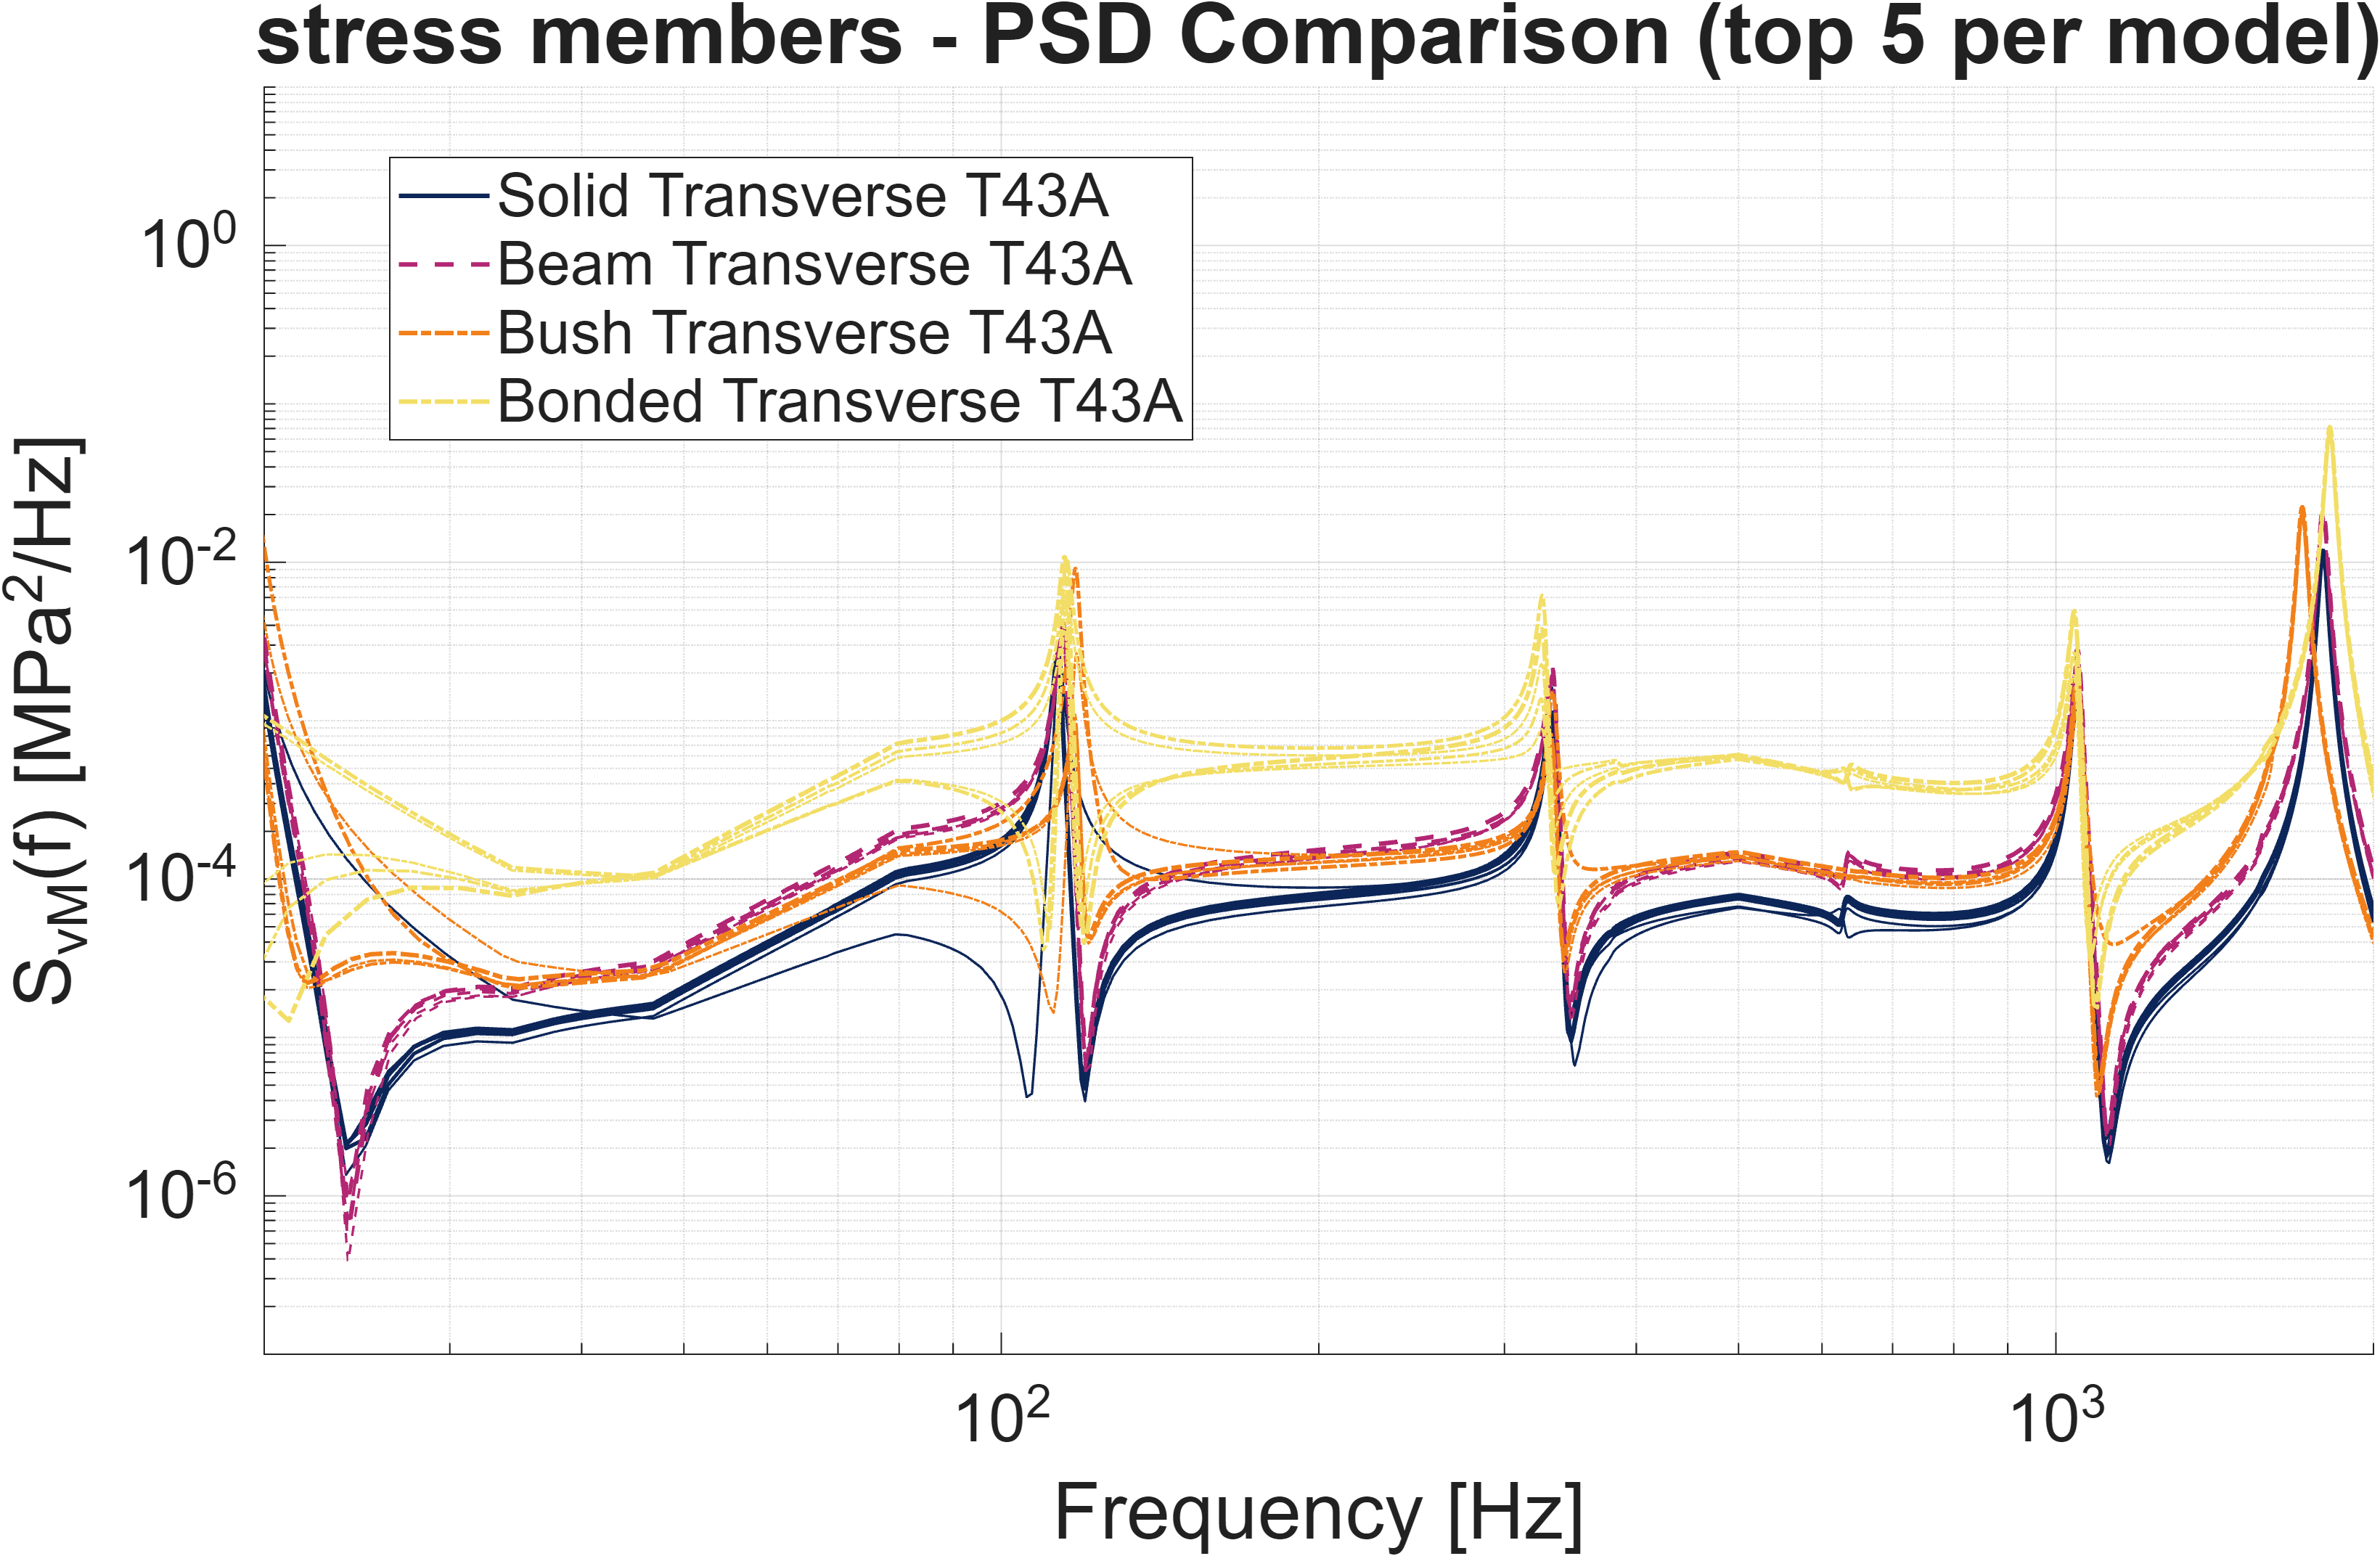
\includegraphics[width=\textwidth]{Transverse T43A/Transverse T43A_psd_overlay_NODEWISE stress_members.png}
        \caption{Transverse Loading (shear).}
        \label{fig:T43A_shear_psd_overlay_NODEWISE_stress_members}
    \end{subfigure}
    \begin{subfigure}[b]{0.45\textwidth}
        \centering
        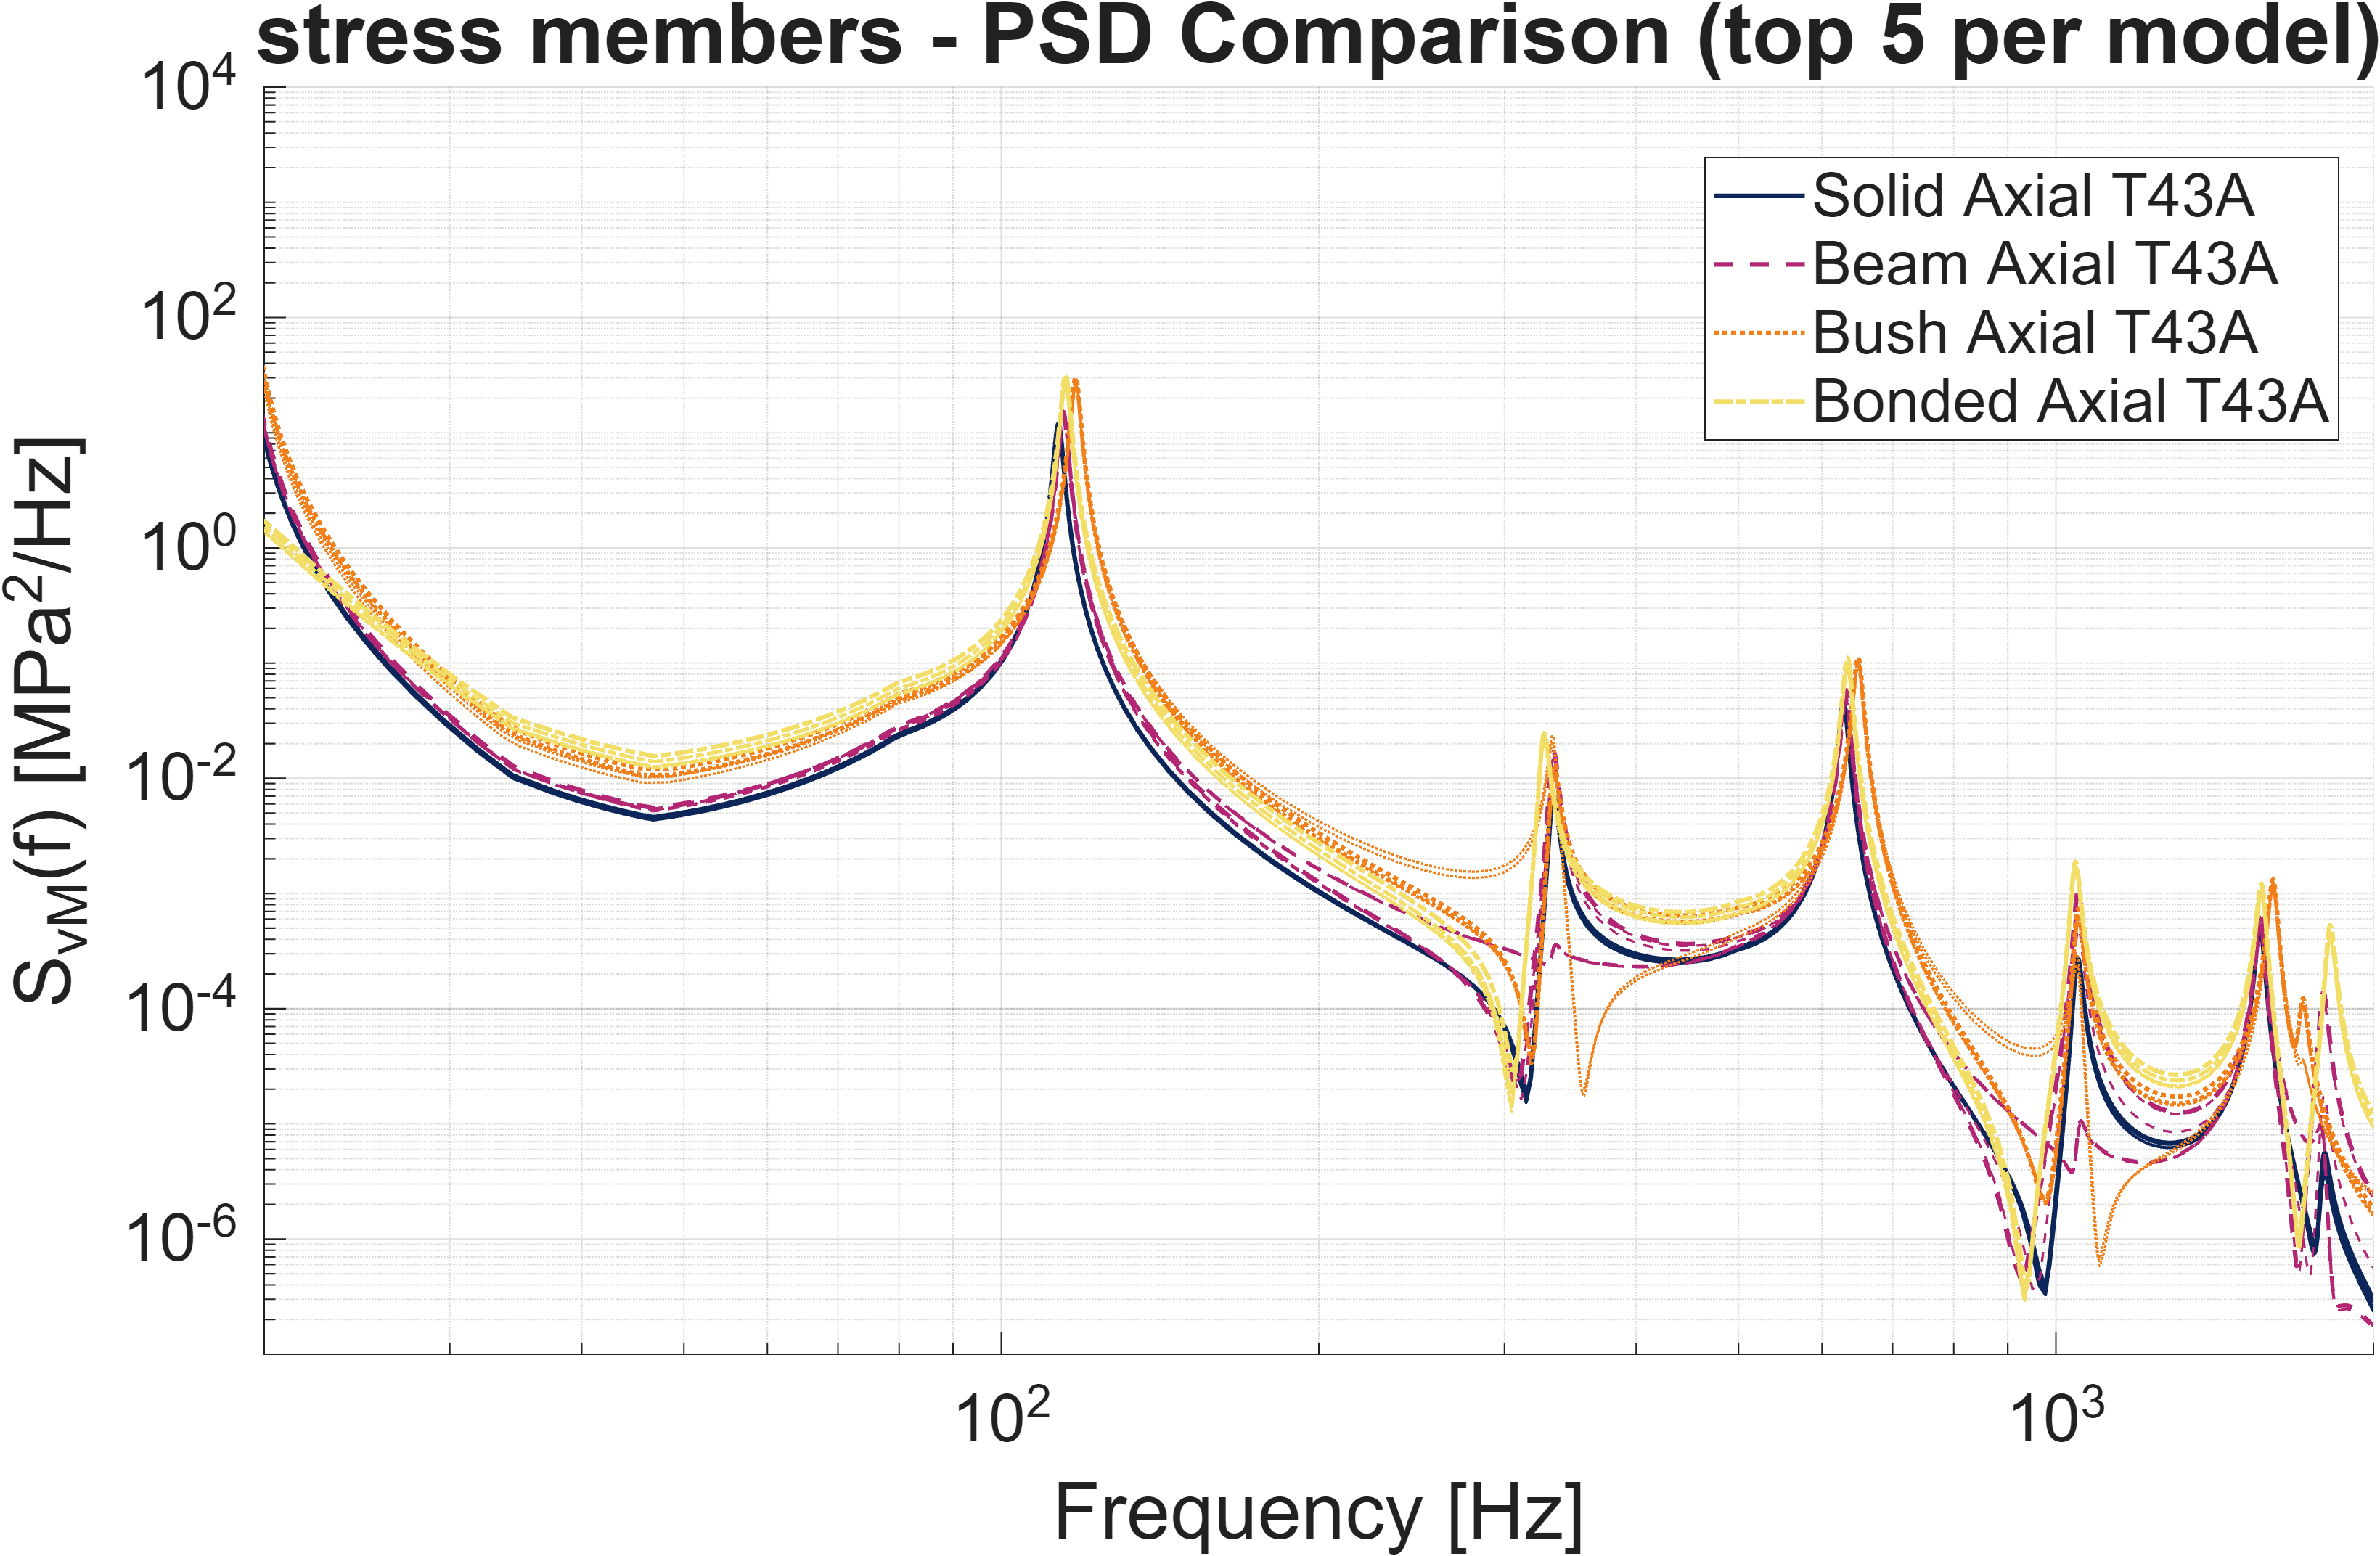
\includegraphics[width=\textwidth]{Axial T43A/Axial T43A_psd_overlay_NODEWISE stress_members.png}
        \caption{Axial Loading (bending).}
        \label{fig:T43A_bending_psd_overlay_NODEWISE_stress_members}
    \end{subfigure}
    
    \caption{Stress PSDs for the \textit{clamped members} (top 5 per model). All models exhibit resonant peaks at the same fundamental frequencies, but the bonded model shows significantly elevated amplitudes for transverse loading. Excited by the MIL-STD 810G profile for T43A.}
    \label{fig:Stress_PSD_Members_Comparison_T43A}
\end{figure}

\begin{figure}[H]
    \centering
    \begin{subfigure}[b]{0.45\textwidth}
        \centering
        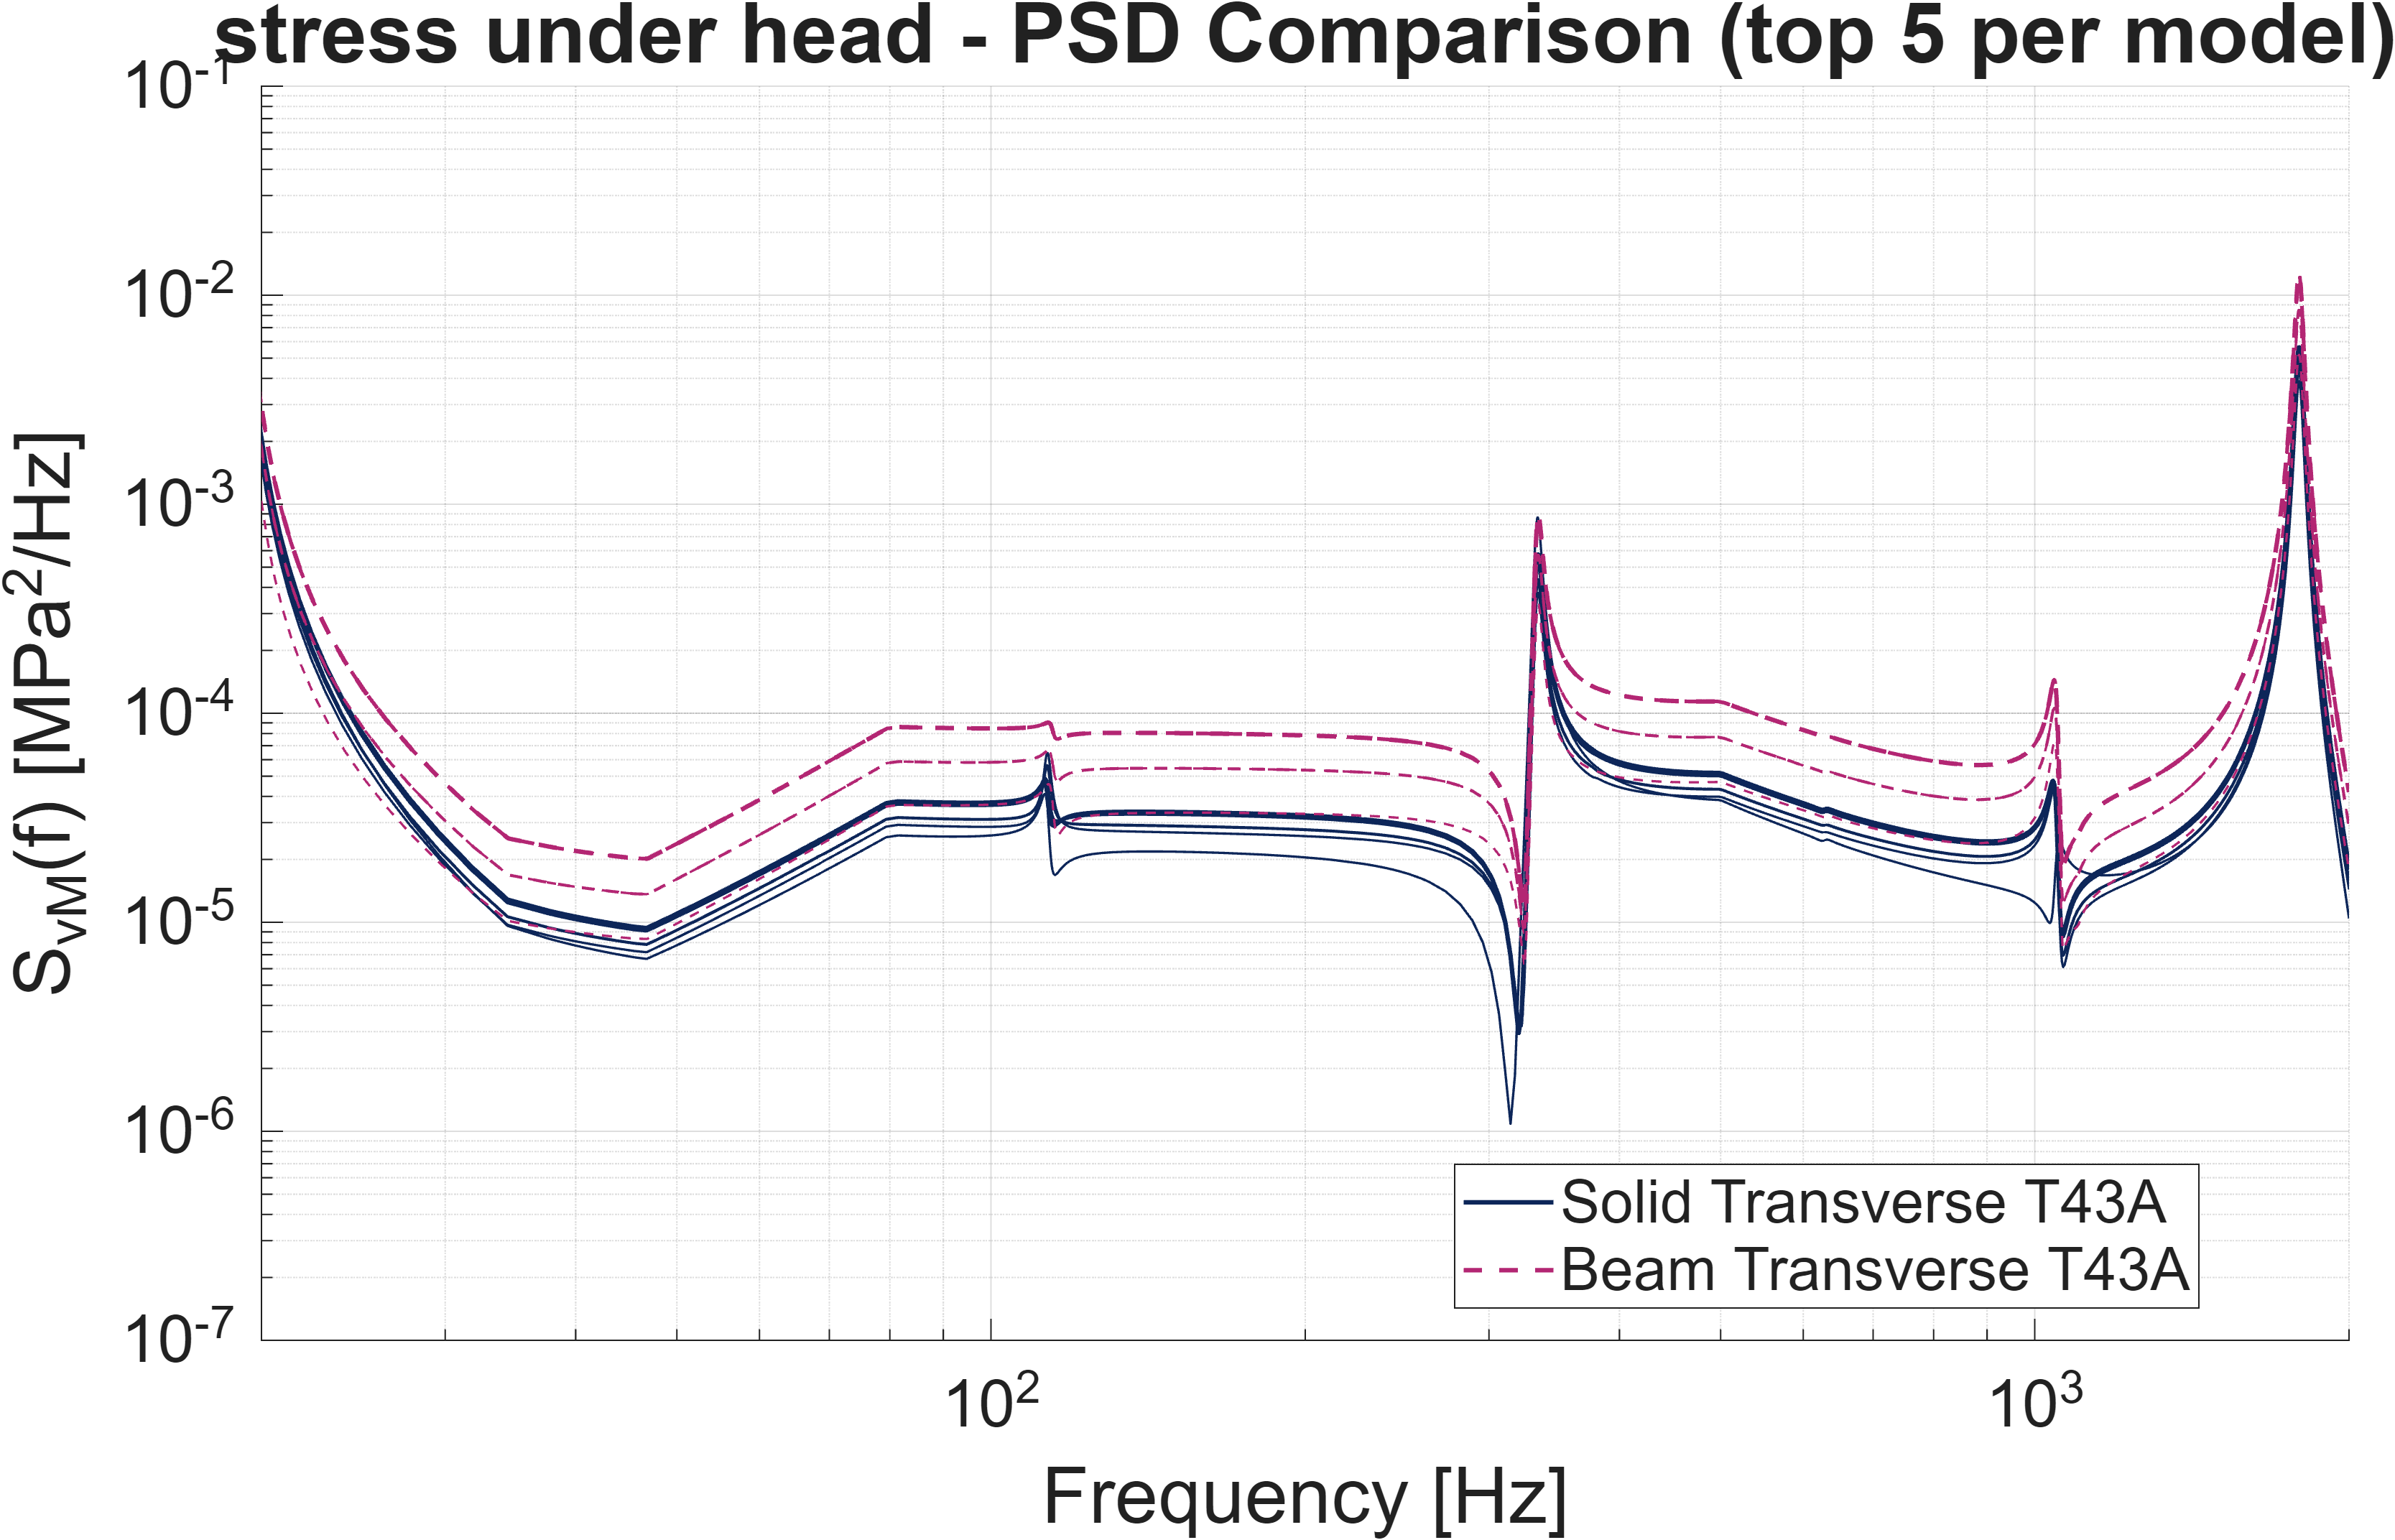
\includegraphics[width=\textwidth]{Transverse T43A/Transverse T43A_psd_overlay_NODEWISE stress_under_head.png}
        \caption{Transverse Loading (shear).}
        \label{fig:T43A_shear_psd_overlay_NODEWISE_stress_under_head}
    \end{subfigure}
    \begin{subfigure}[b]{0.45\textwidth}
        \centering
        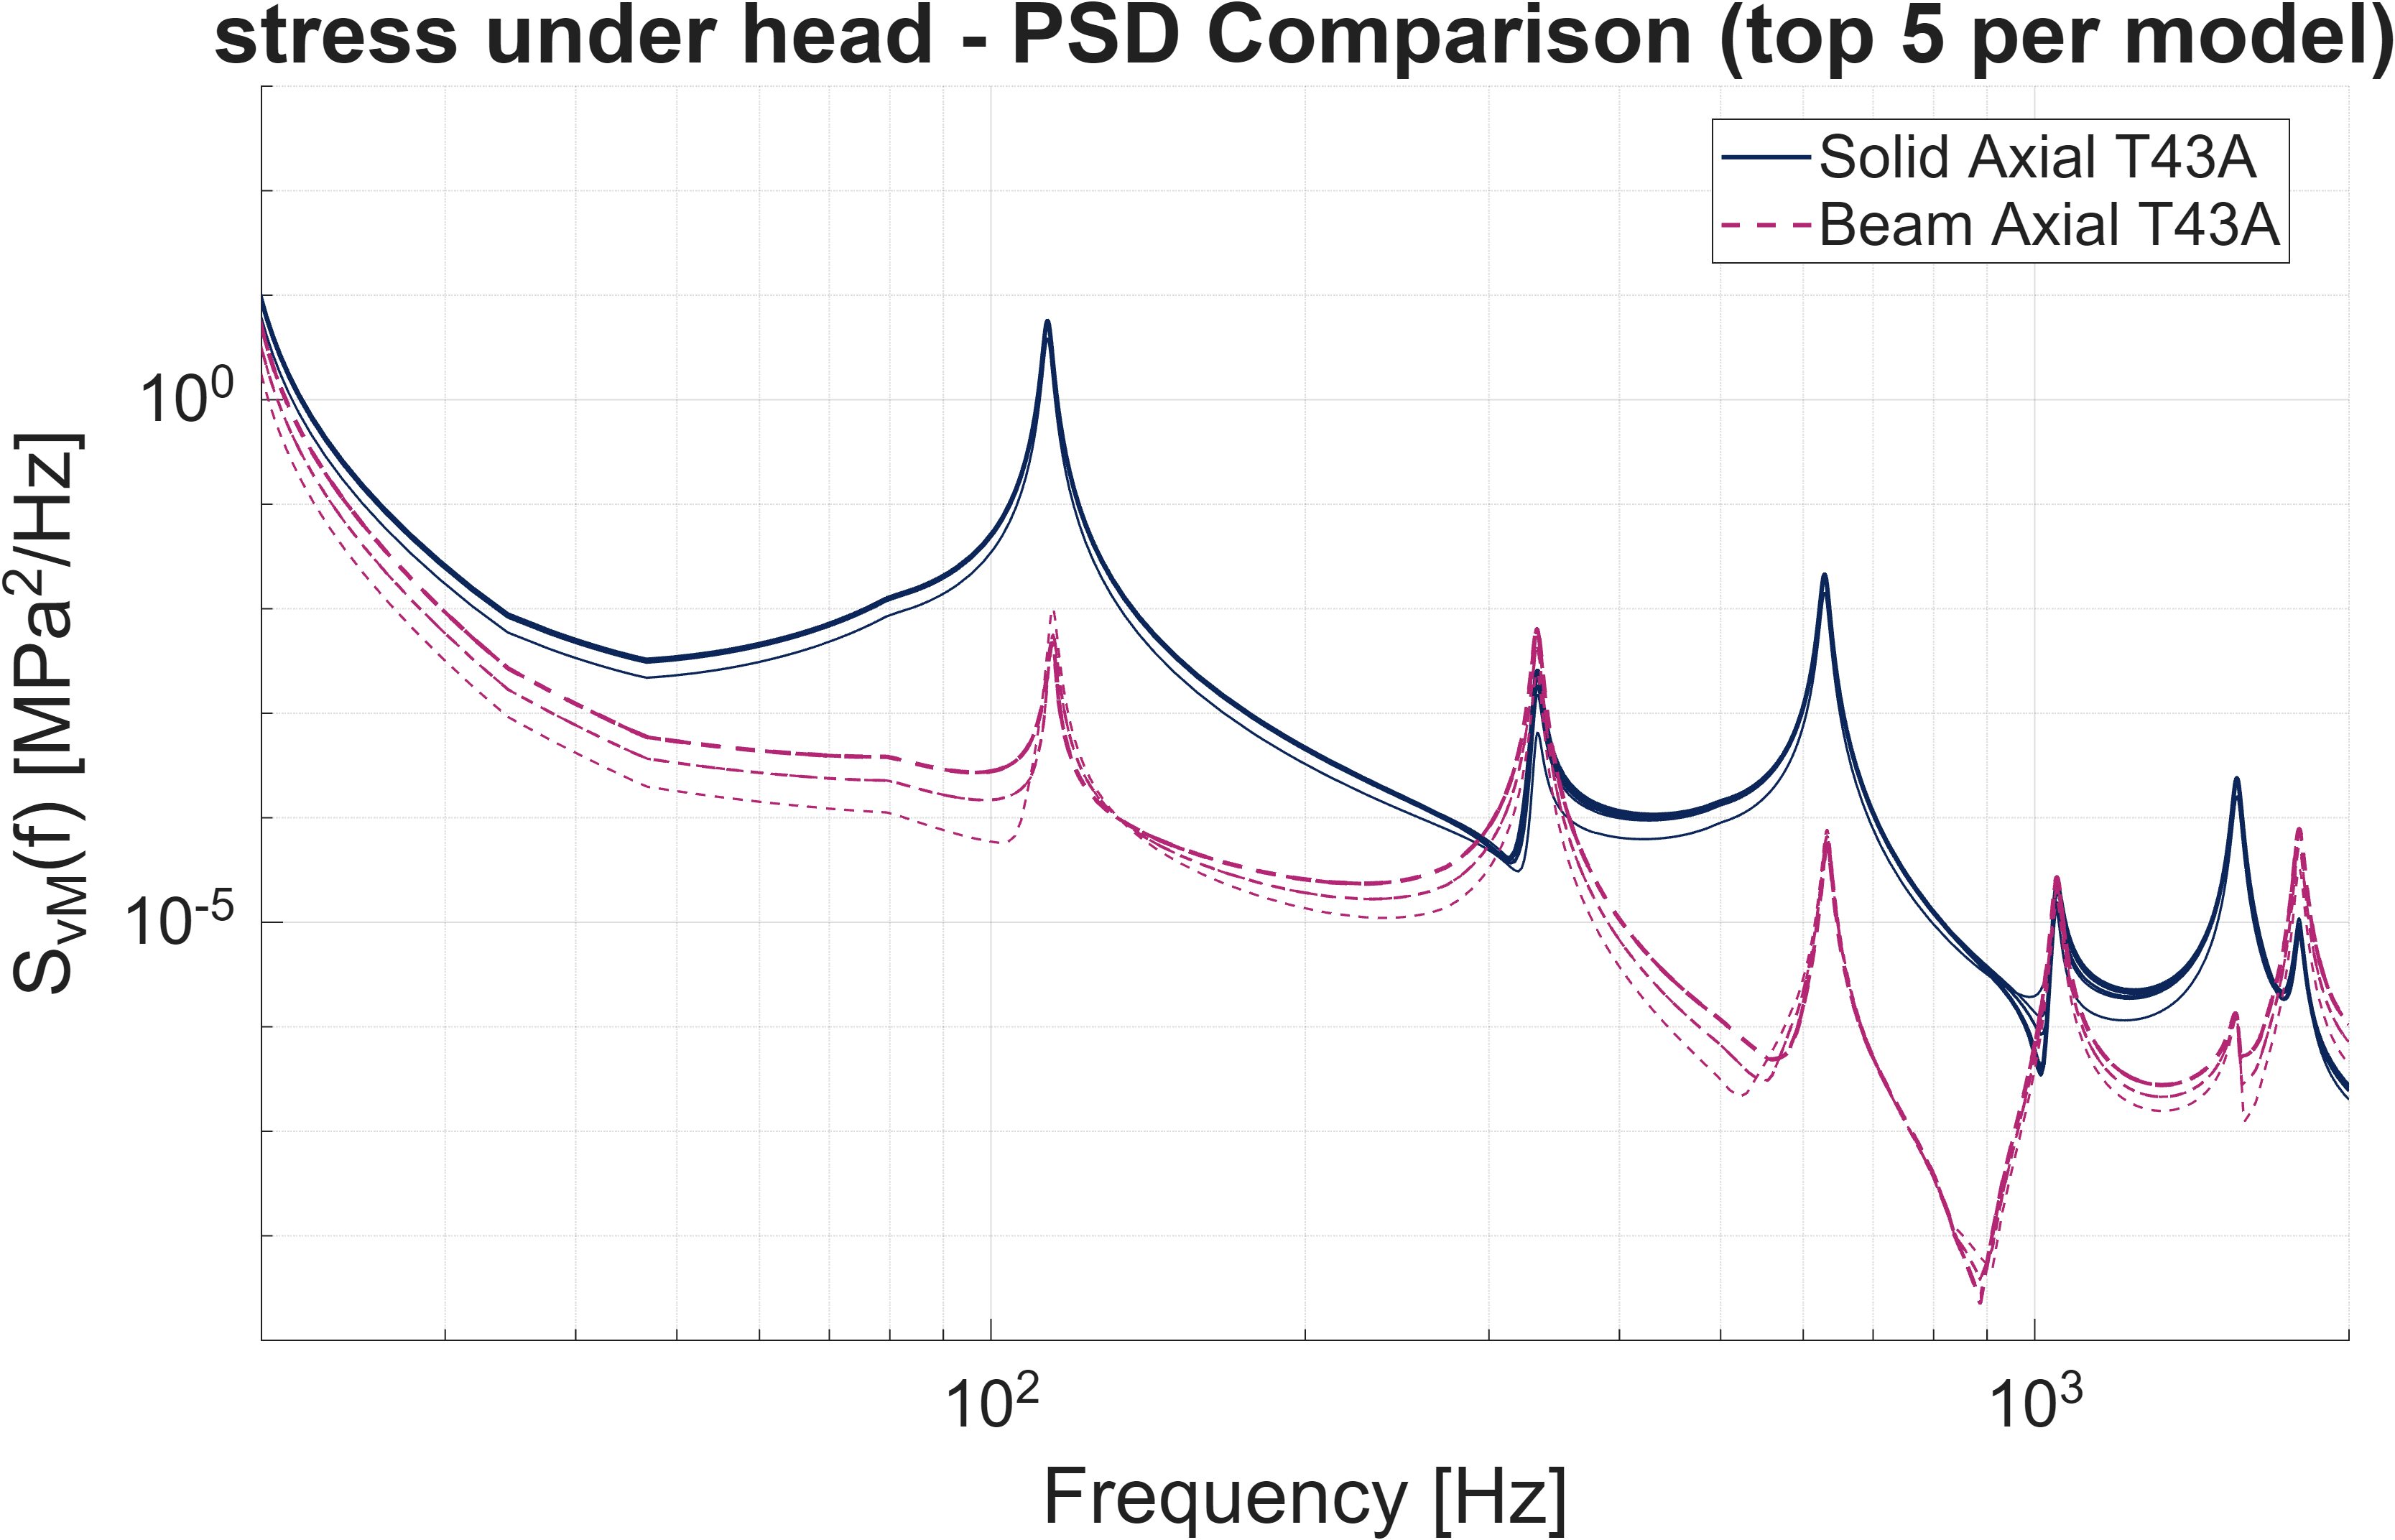
\includegraphics[width=\textwidth]{Axial T43A/Axial T43A_psd_overlay_NODEWISE stress_under_head.png}
        \caption{Axial Loading (bending).}
        \label{fig:T43A_bending_psd_overlay_NODEWISE_stress_under_head}
    \end{subfigure}
    
    \caption{Stress PSDs for the \textit{stress under-head fillet} (top 5 nodes per model). Left: transverse loading, right: axial loading. The beam model returns non-zero stress in both directions, but deviates from the solid under axial loading. Excited by the MIL-STD 810G profile for T43A.}
    \label{fig:Stress_PSD_UnderHead_Comparison_T43A}
\end{figure}

\begin{figure}[H]
    \centering
    \begin{subfigure}[b]{0.45\textwidth}
        \centering
        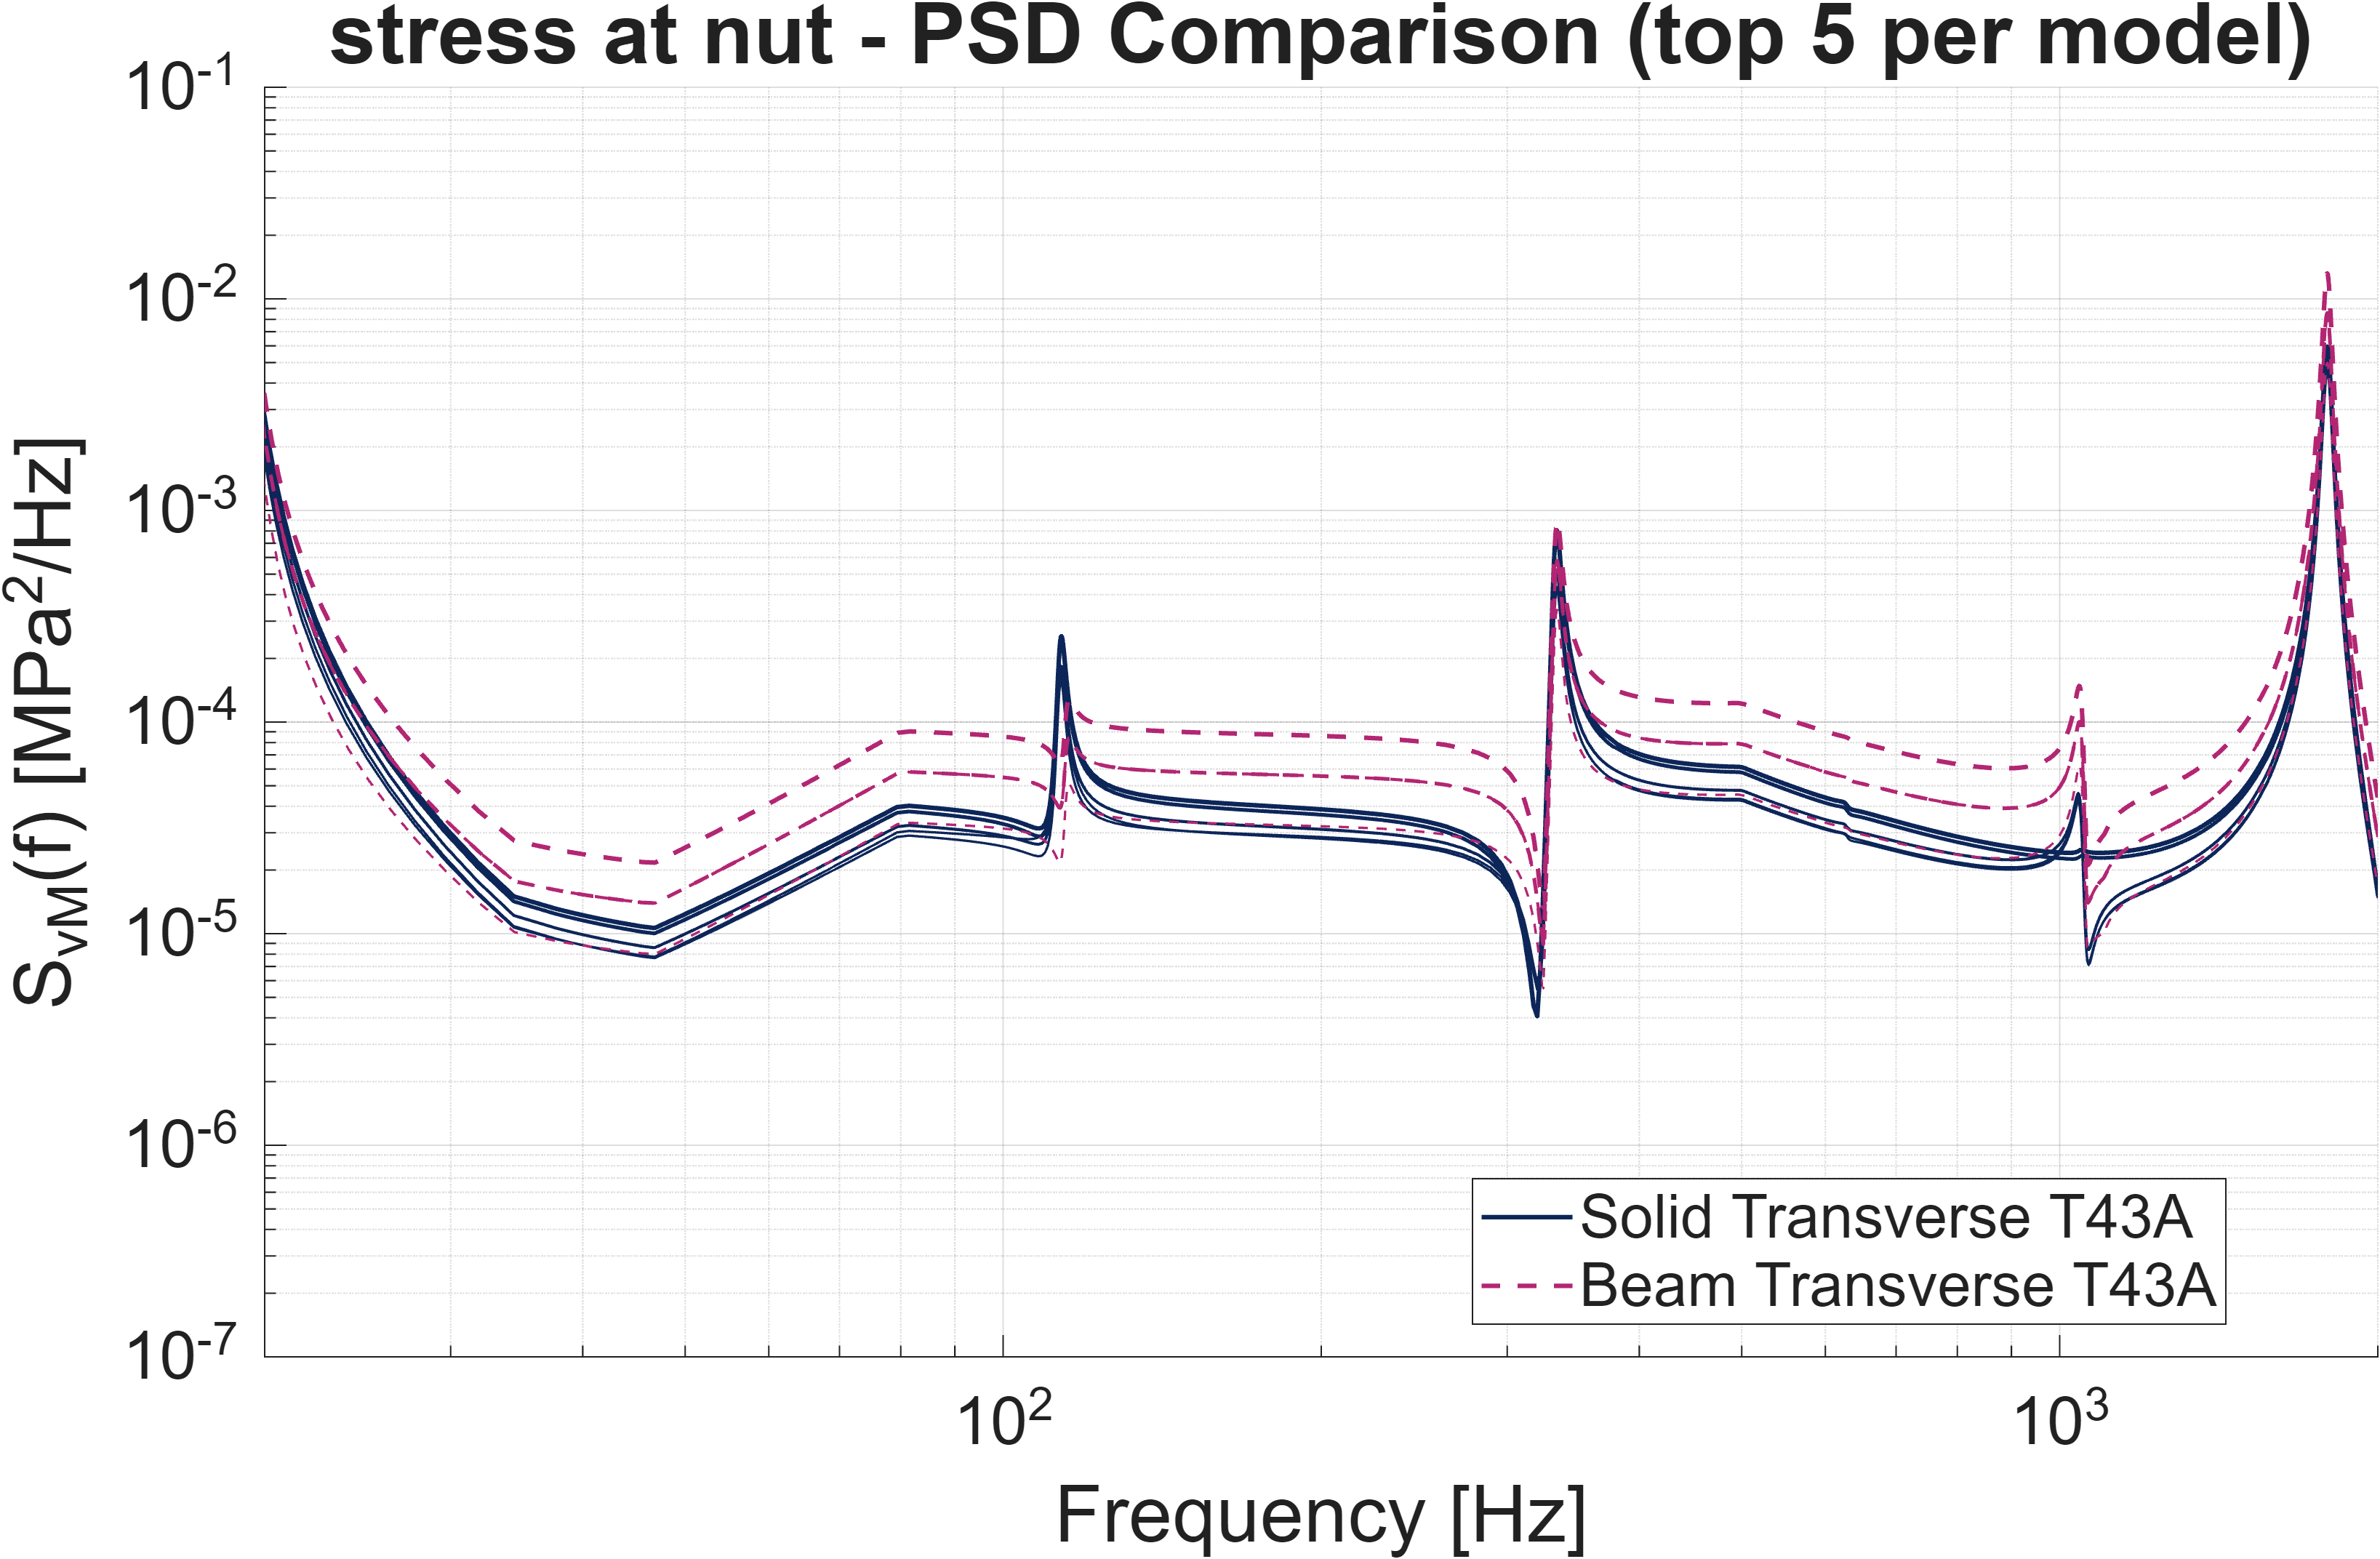
\includegraphics[width=\textwidth]{Transverse T43A/Transverse T43A_psd_overlay_NODEWISE stress_at_nut.png}
        \caption{Transverse Loading (shear).}
        \label{fig:T43A_shear_psd_overlay_NODEWISE_stress_at_nut}
    \end{subfigure}
    \begin{subfigure}[b]{0.45\textwidth}
        \centering
        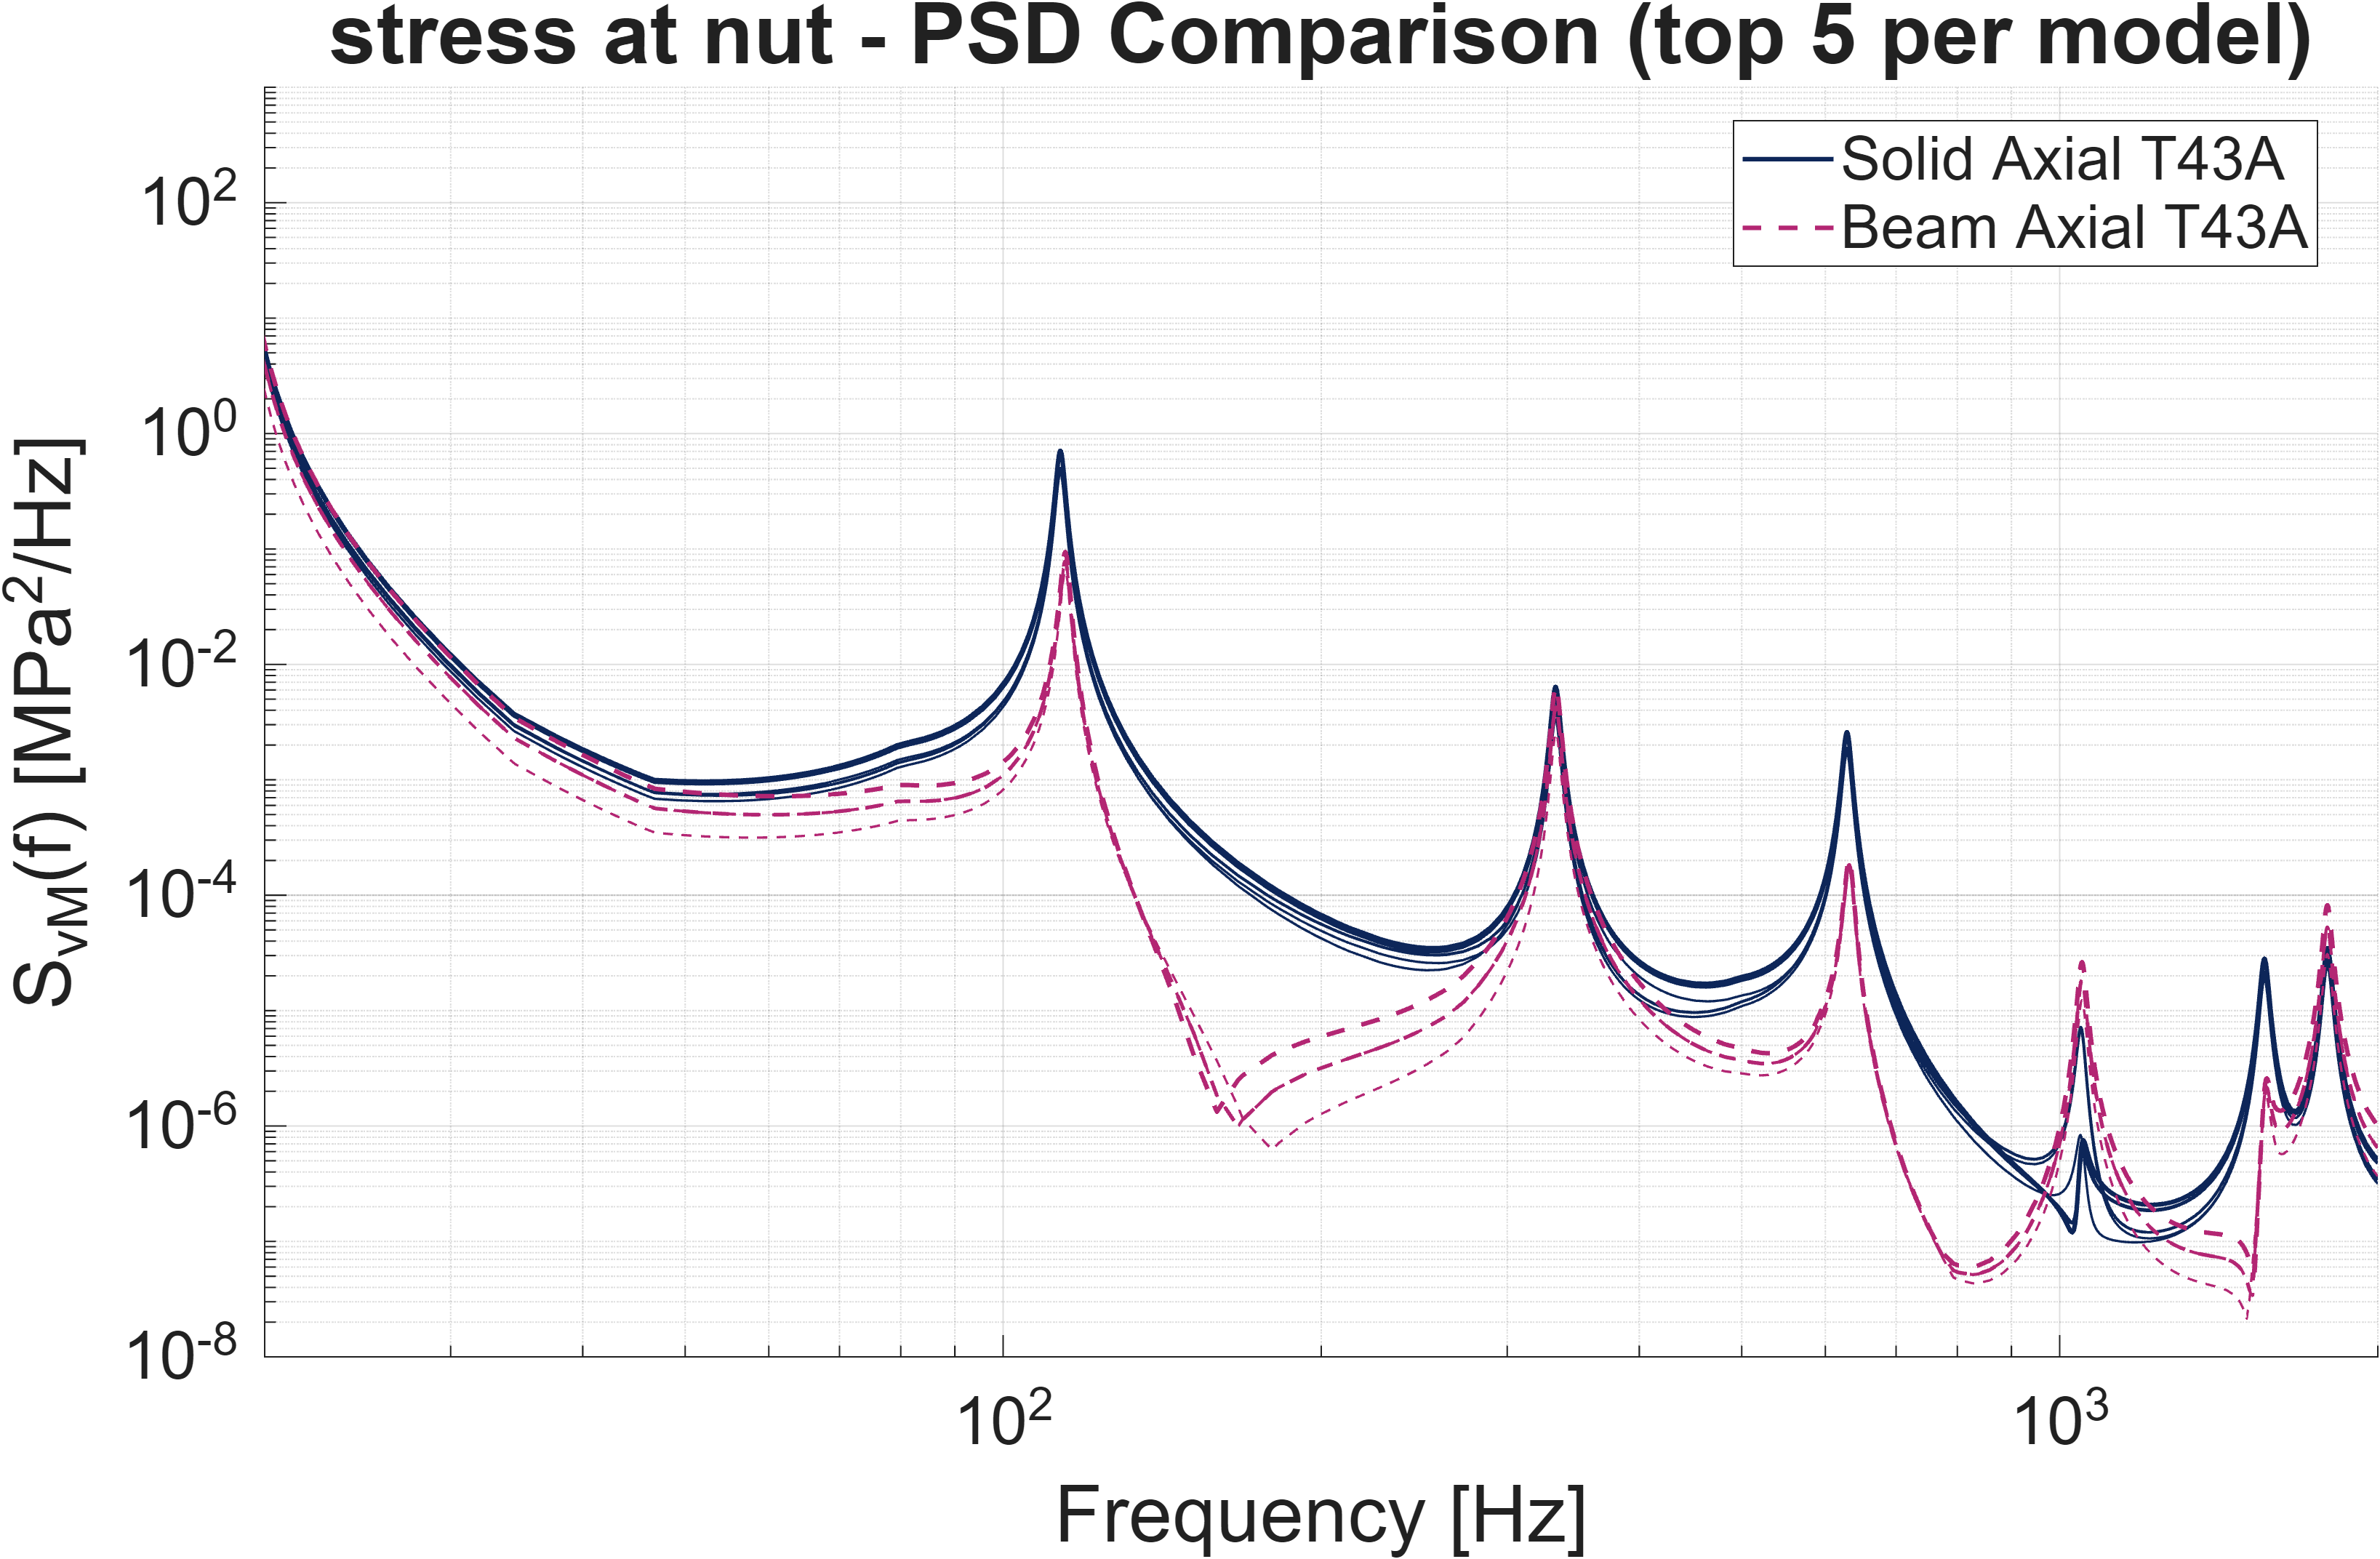
\includegraphics[width=\textwidth]{Axial T43A/Axial T43A_psd_overlay_NODEWISE stress_at_nut.png}
        \caption{Axial Loading (bending).}
        \label{fig:T43A_bending_psd_overlay_NODEWISE_stress_at_nut}
    \end{subfigure}
    
    \caption{Stress \ac{PSD} for the \textit{stress at nut} (top 5 nodes per model). Both models predict finite stress, the beam overpredicts the \ac{RMS} under transverse loading and underpredicts under axial loading relative to the solid. Excited by the MIL-STD 810G profile for T43A.}
    \label{fig:Stress_PSD_AtNut_Comparison_T43A}
\end{figure}

\begin{figure}[H]
    \centering
    \begin{subfigure}[b]{0.45\textwidth}
        \centering
        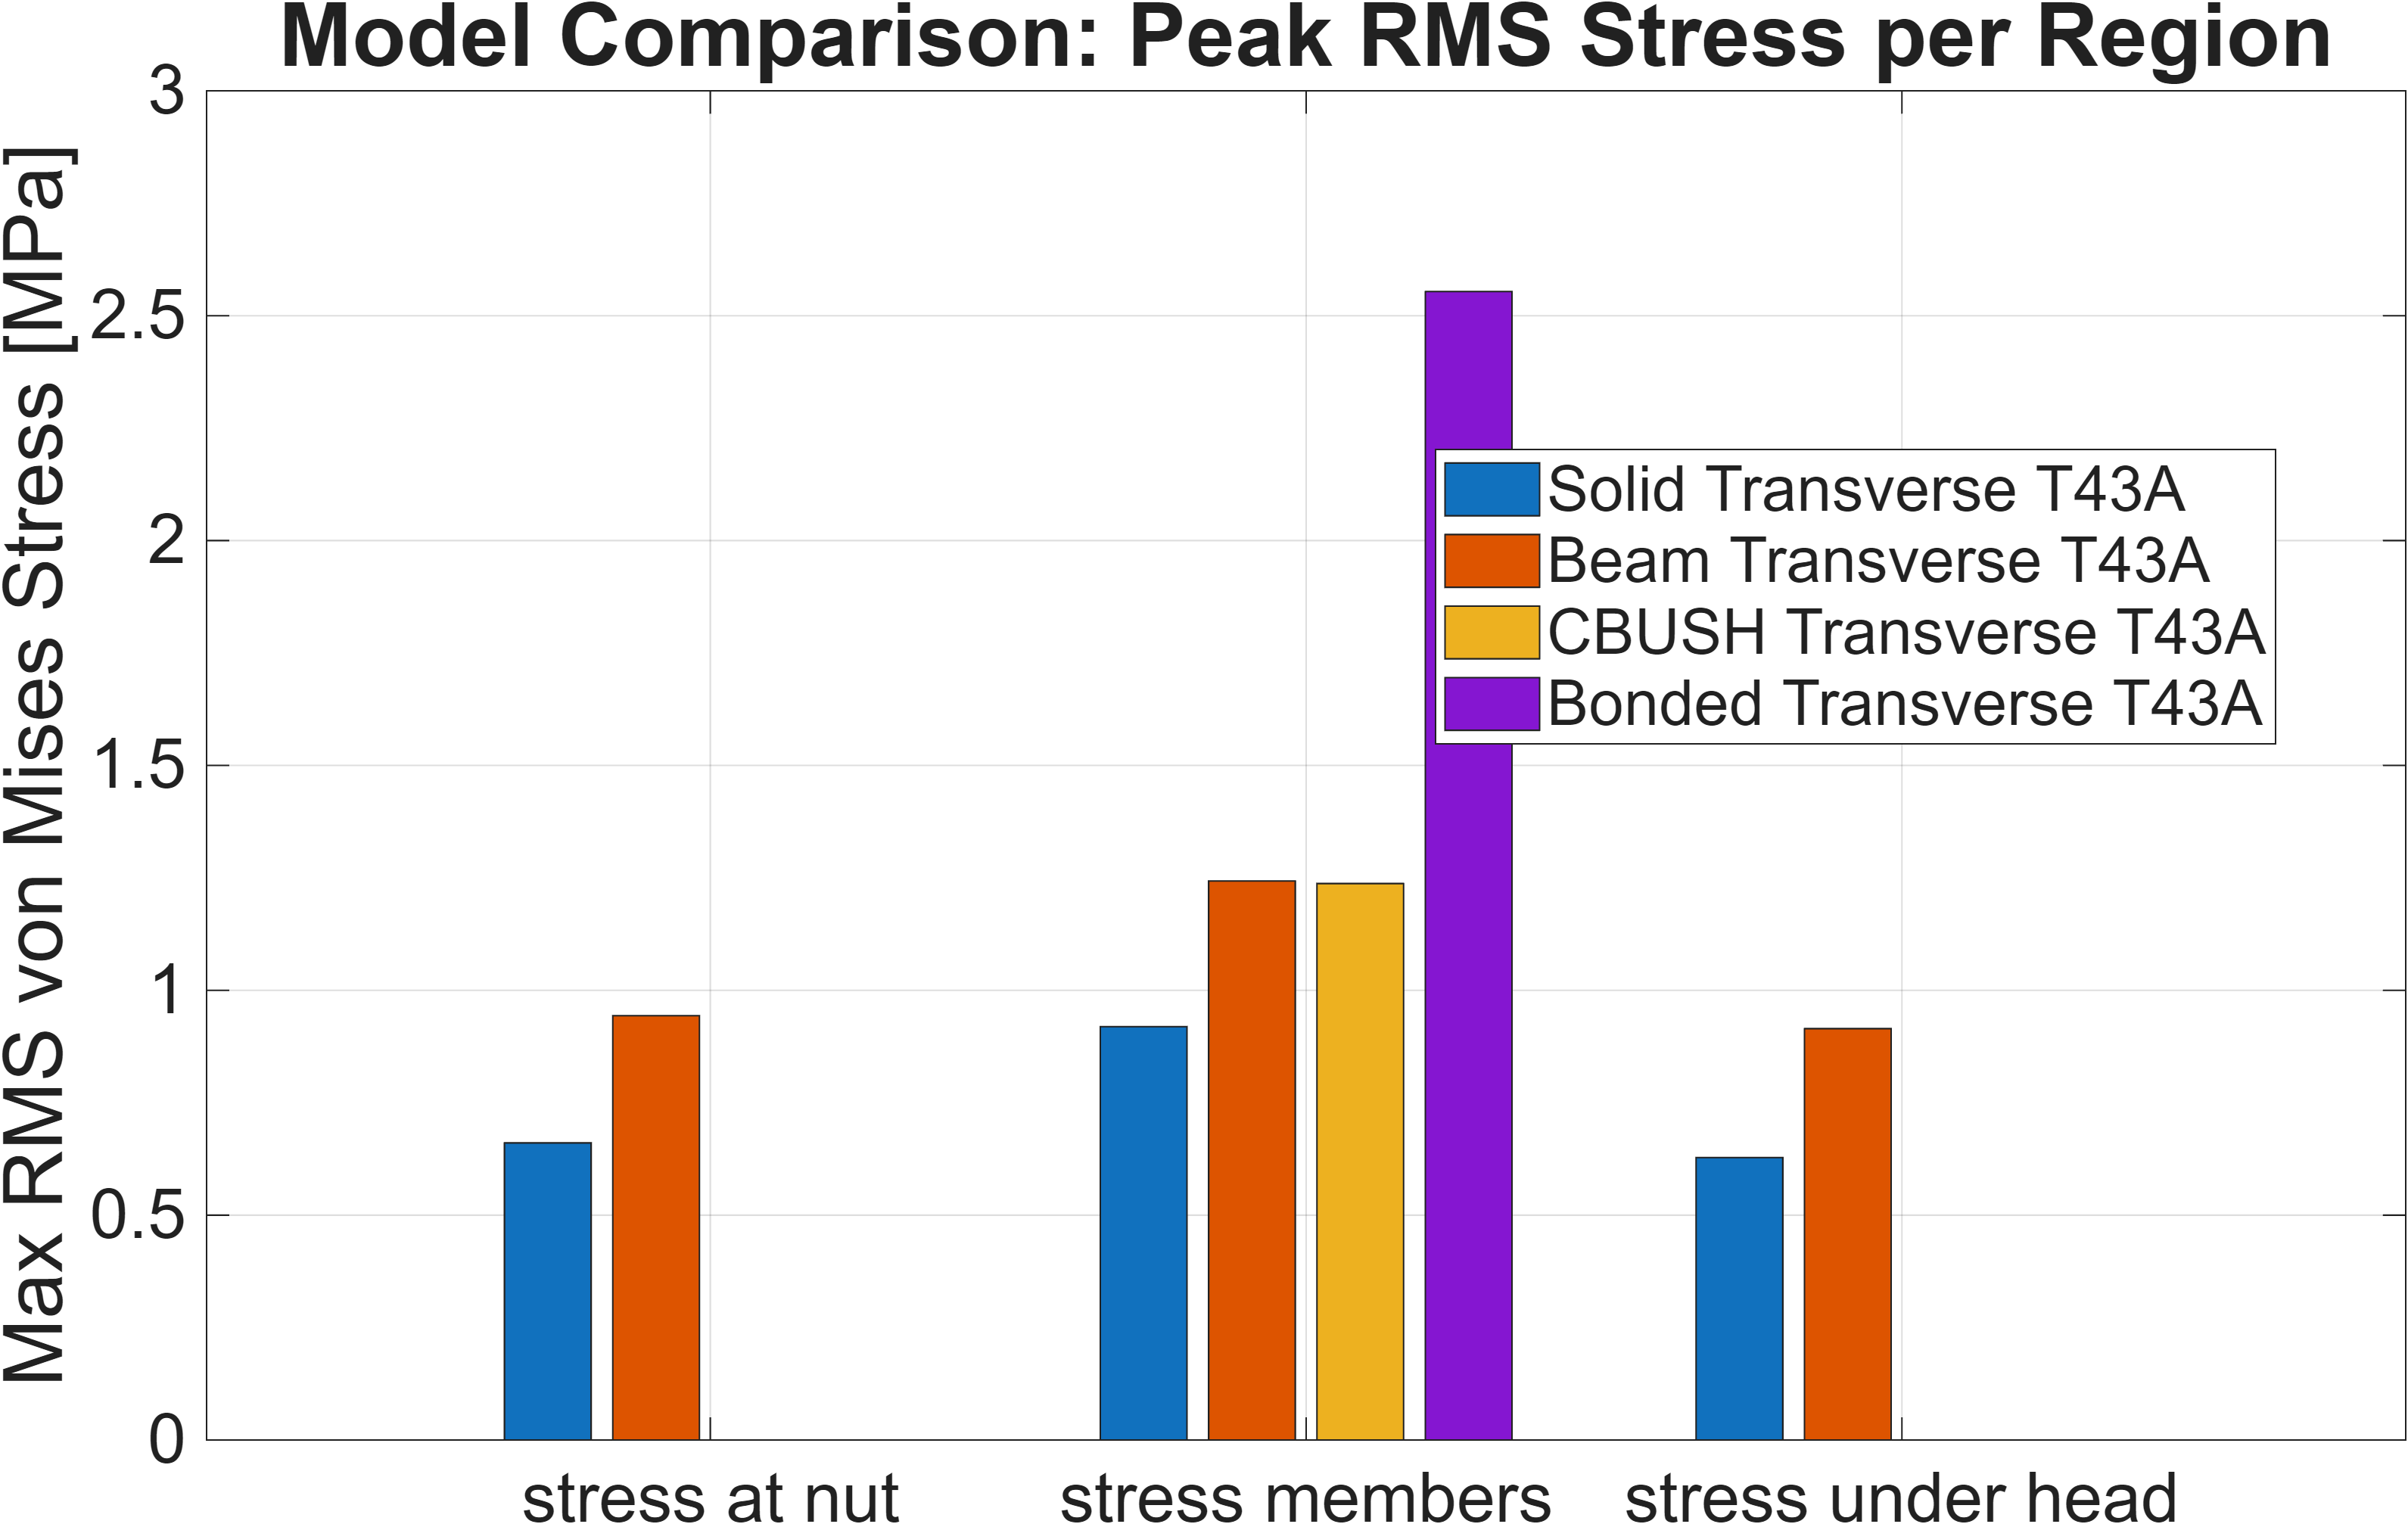
\includegraphics[width=\textwidth]{Transverse T43A/Transverse T43A_comparison_max_rms_per_region NODEWISE.png}
        \caption{Transverse Loading (shear).}
        \label{fig:T43A_shear_comparison_max_rms_per_region_NODEWISE}
    \end{subfigure}
    \begin{subfigure}[b]{0.45\textwidth}
        \centering
        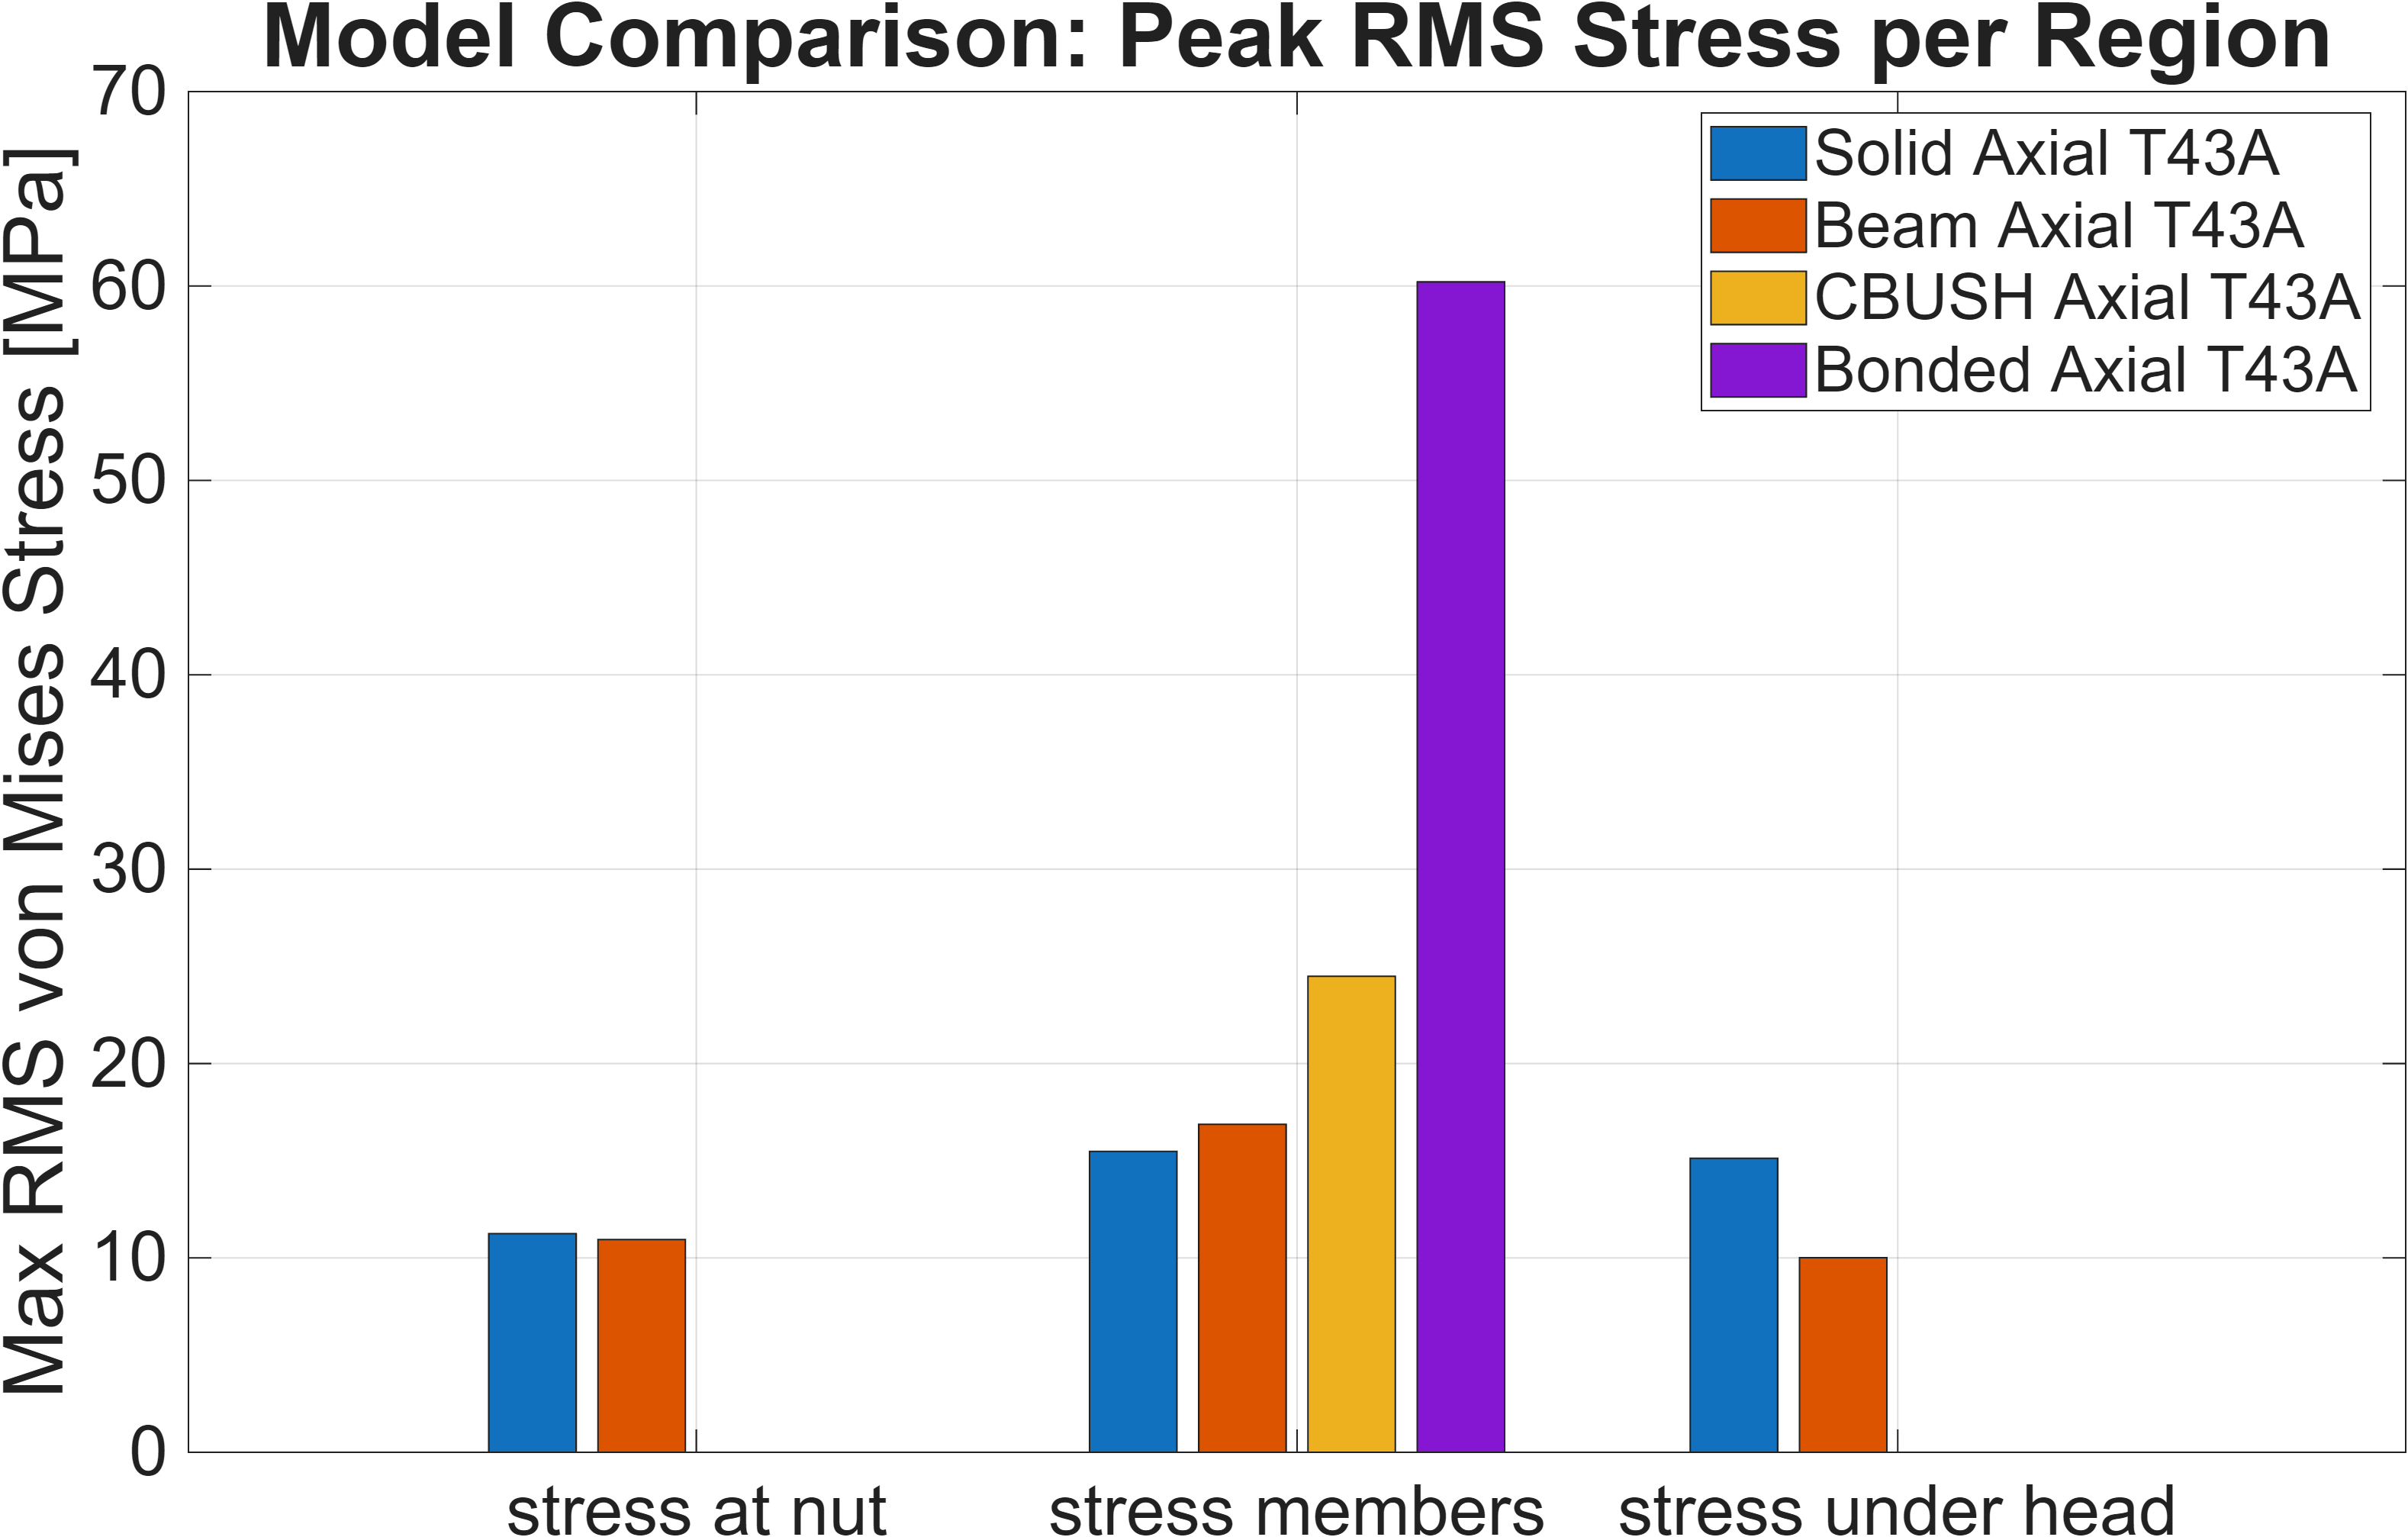
\includegraphics[width=\textwidth]{Axial T43A/Axial T43A_comparison_max_rms_per_region NODEWISE.png}
        \caption{Axial Loading (bending).}
        \label{fig:T43A_bending_comparison_max_rms_per_region_NODEWISE}
    \end{subfigure}
    
    \caption{Maximum \ac{RMS} von Mises stress per region and model. Excited by the MIL-STD 810G profile for T43A.}
    \label{fig:RMS_per_region_T43A}
\end{figure}

\begin{figure}[H]
    \centering
    \begin{subfigure}[b]{0.45\textwidth}
        \centering
        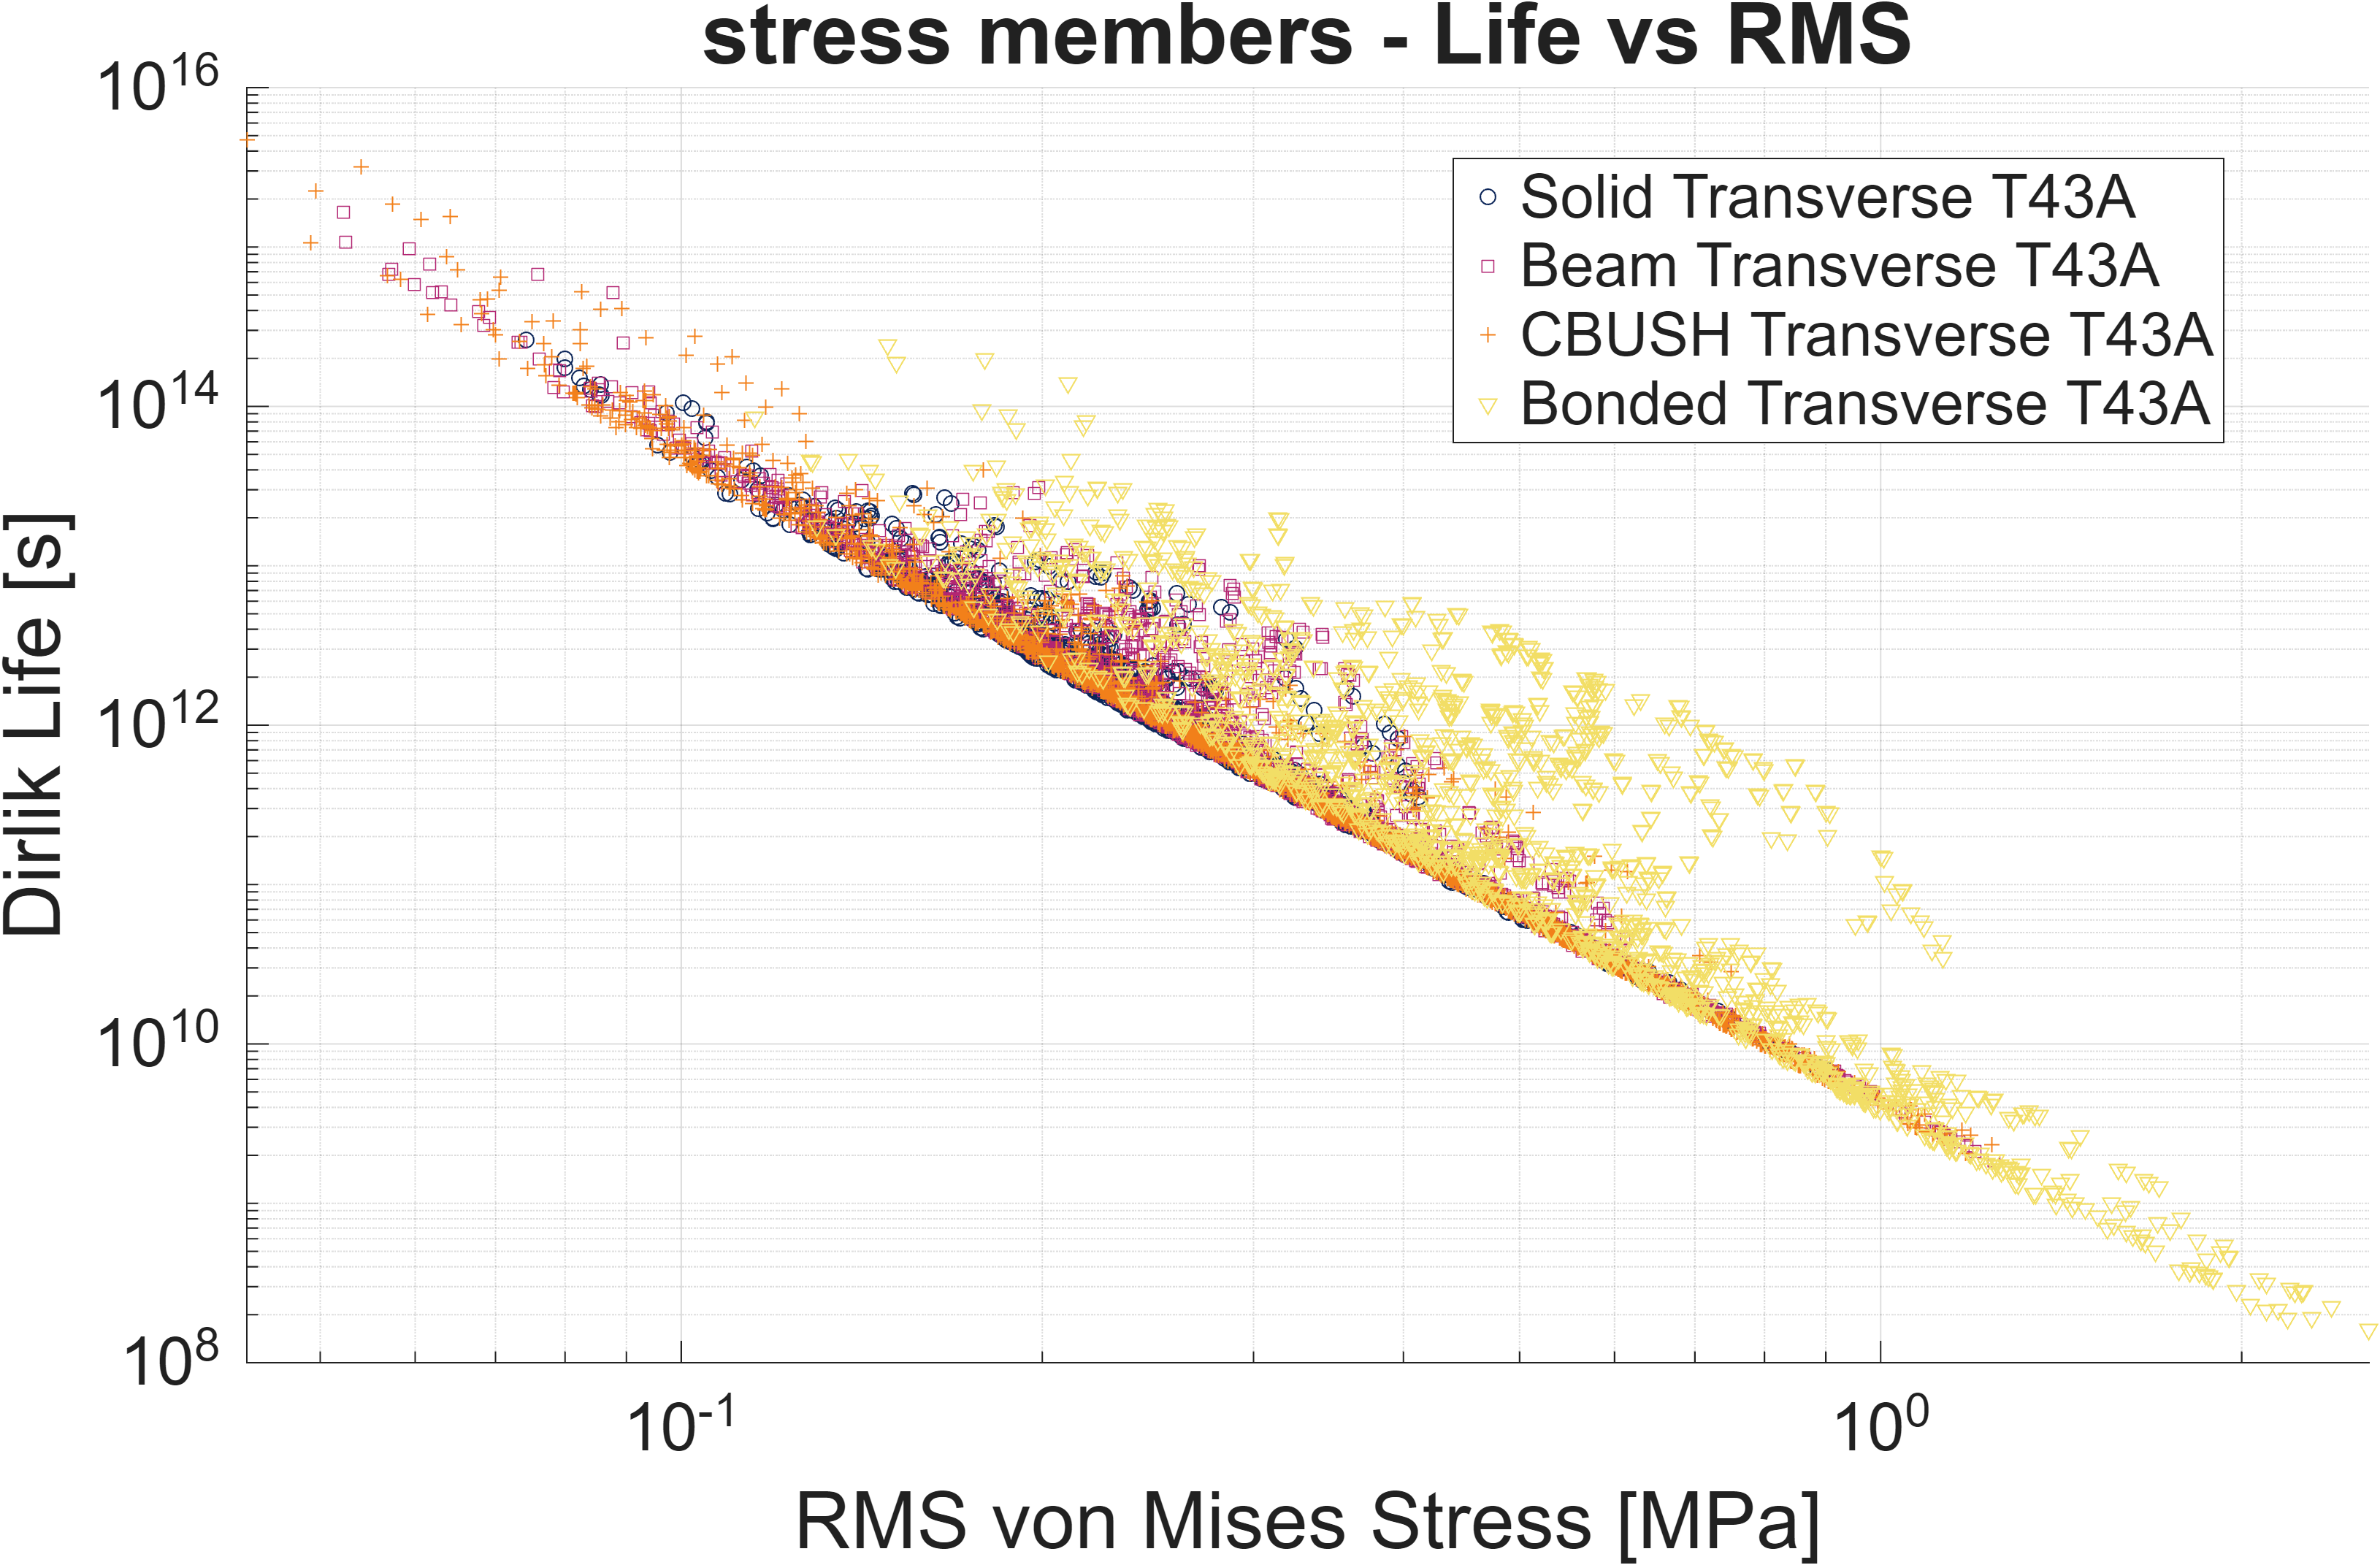
\includegraphics[width=\textwidth]{Transverse T43A/Transverse T43A_life_vs_rms_NODEWISE stress_members.png}
        \caption{Transverse Loading (shear).}
        \label{fig:T43A_shear_life_vs_rms_NODEWISE_stress_members}
    \end{subfigure}
    \begin{subfigure}[b]{0.45\textwidth}
        \centering
        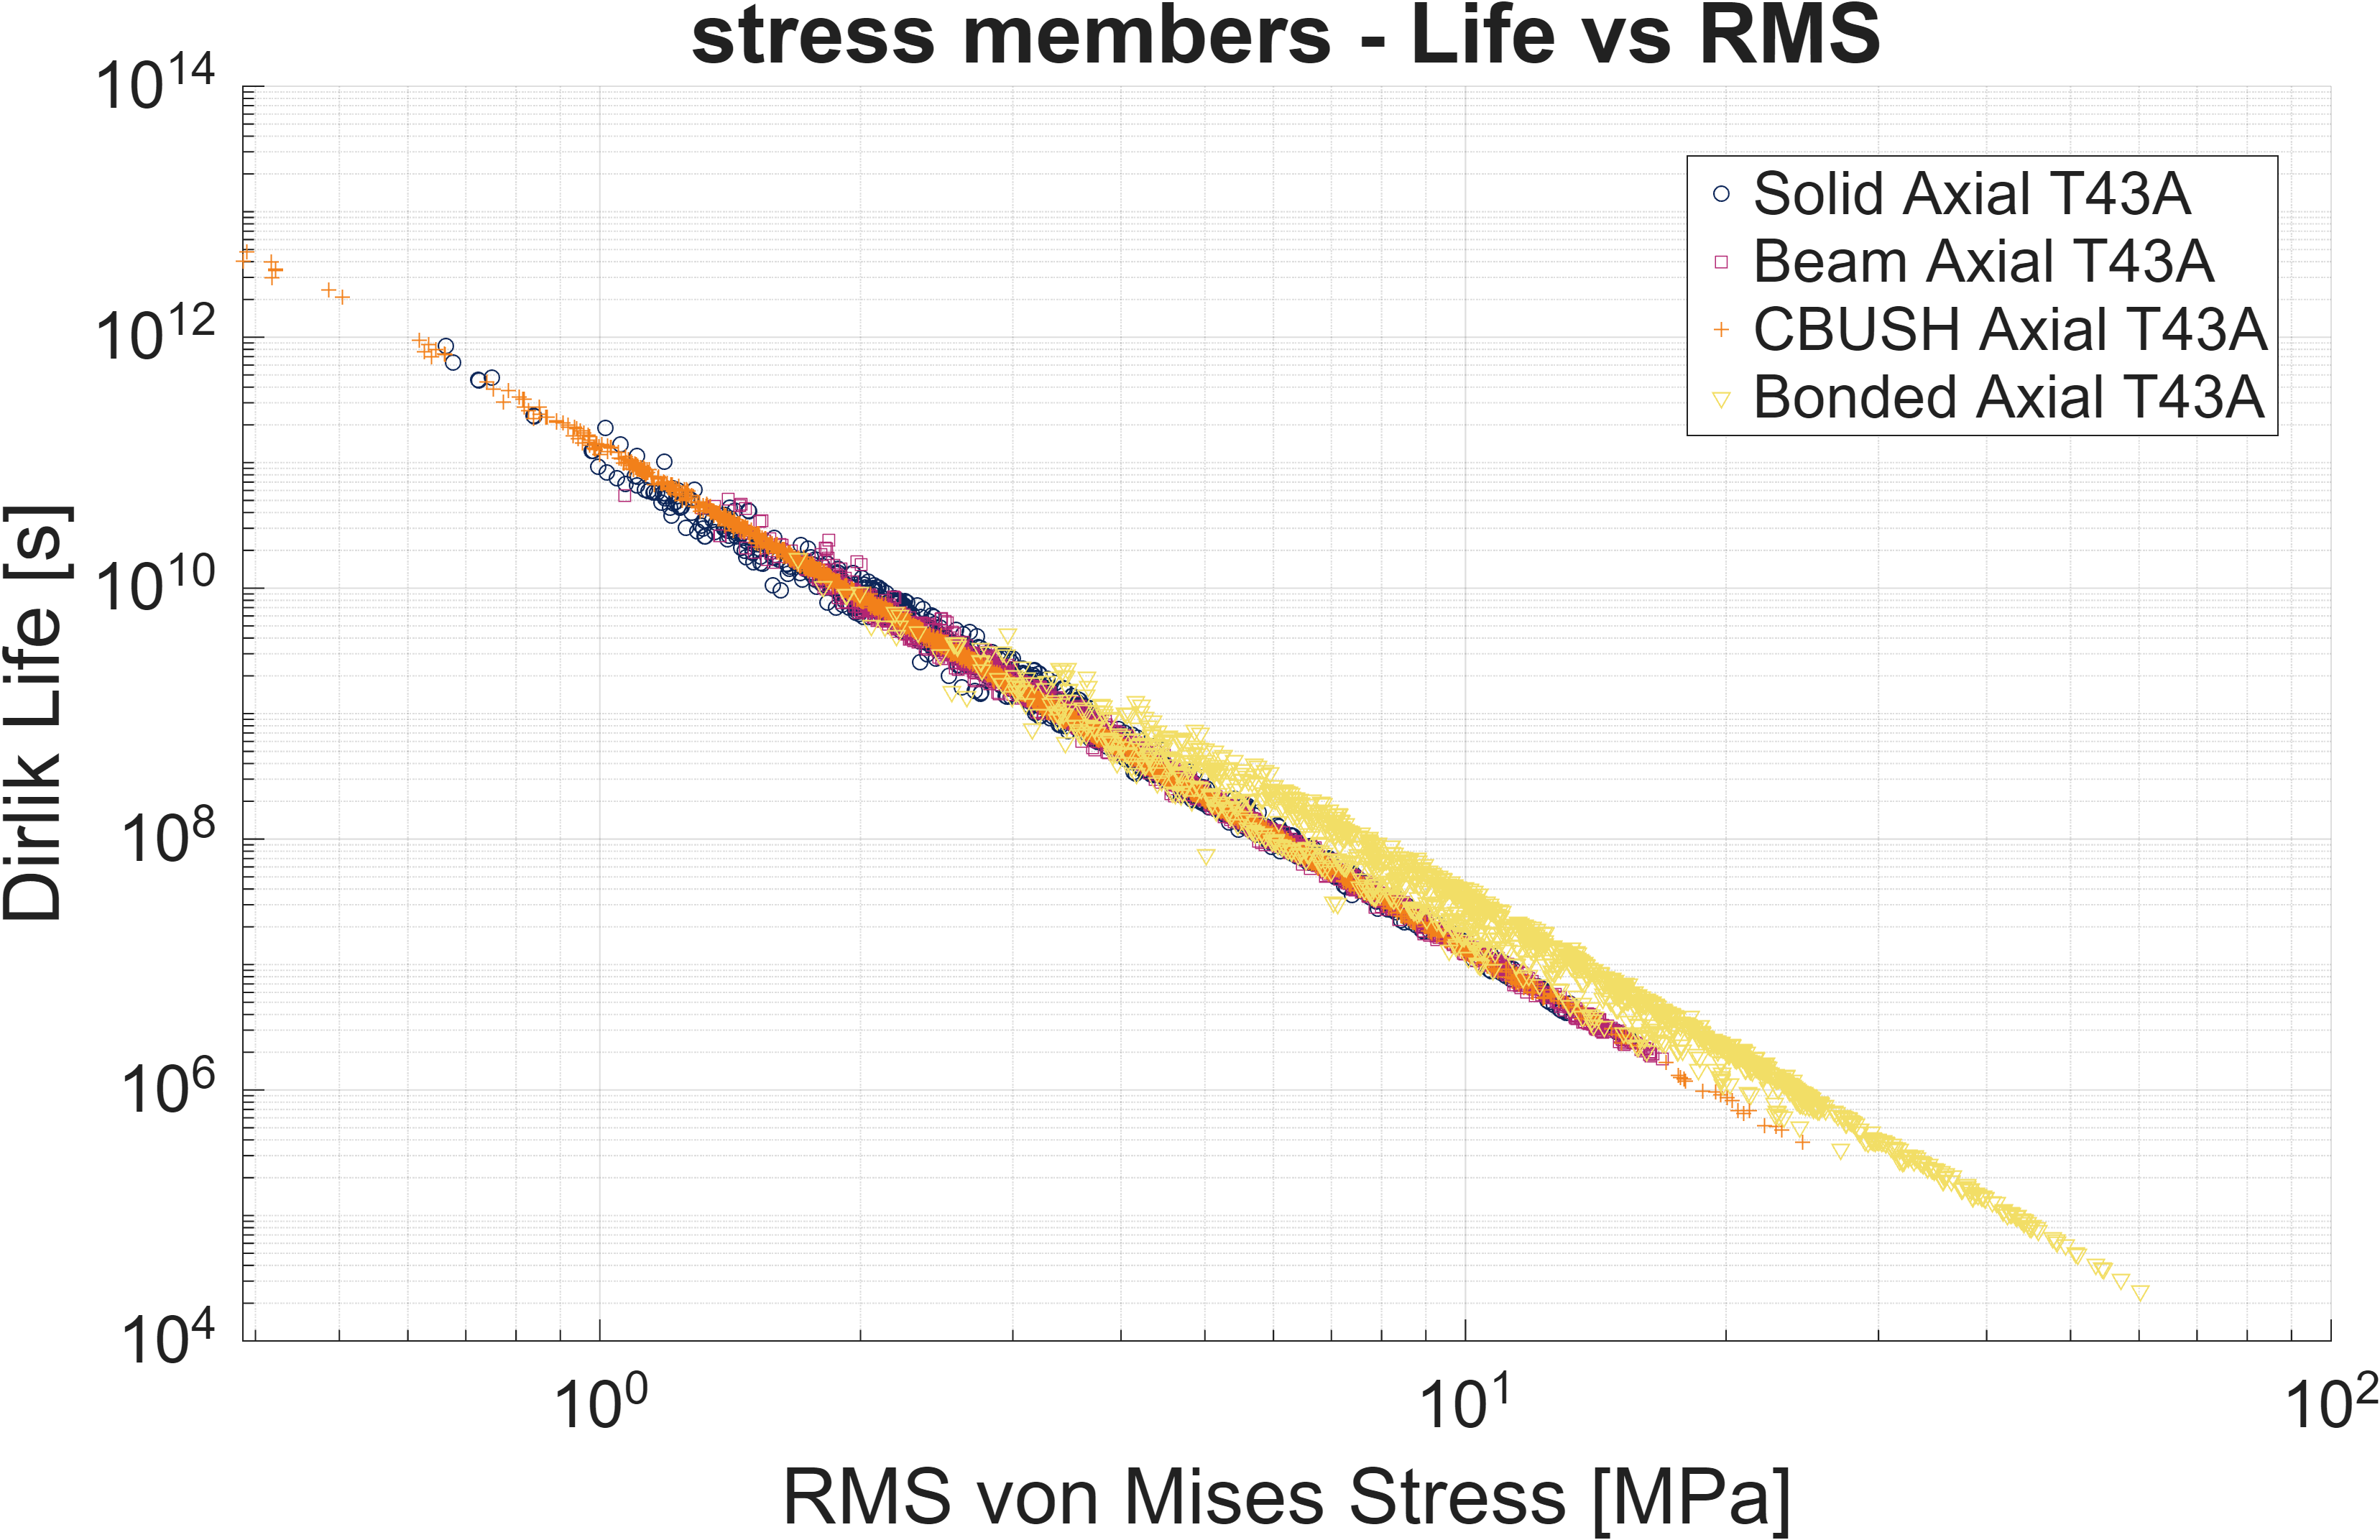
\includegraphics[width=\textwidth]{Axial T43A/Axial T43A_life_vs_rms_NODEWISE stress_members.png}
        \caption{Axial Loading (bending).}
        \label{fig:T43A_bending_life_vs_rms_NODEWISE_stress_members}
    \end{subfigure}
    
    \caption{Dirlik life versus \ac{RMS} stress for the clamped members. The bonded model gives the highest \ac{RMS} and therefore also the shortest life. Excited by the MIL-STD 810G profile for T43A.}
    \label{fig:Life_VS_RMS_members_T43A}
\end{figure}

\begin{figure}[H]
    \centering
    \begin{subfigure}[b]{0.45\textwidth}
        \centering
        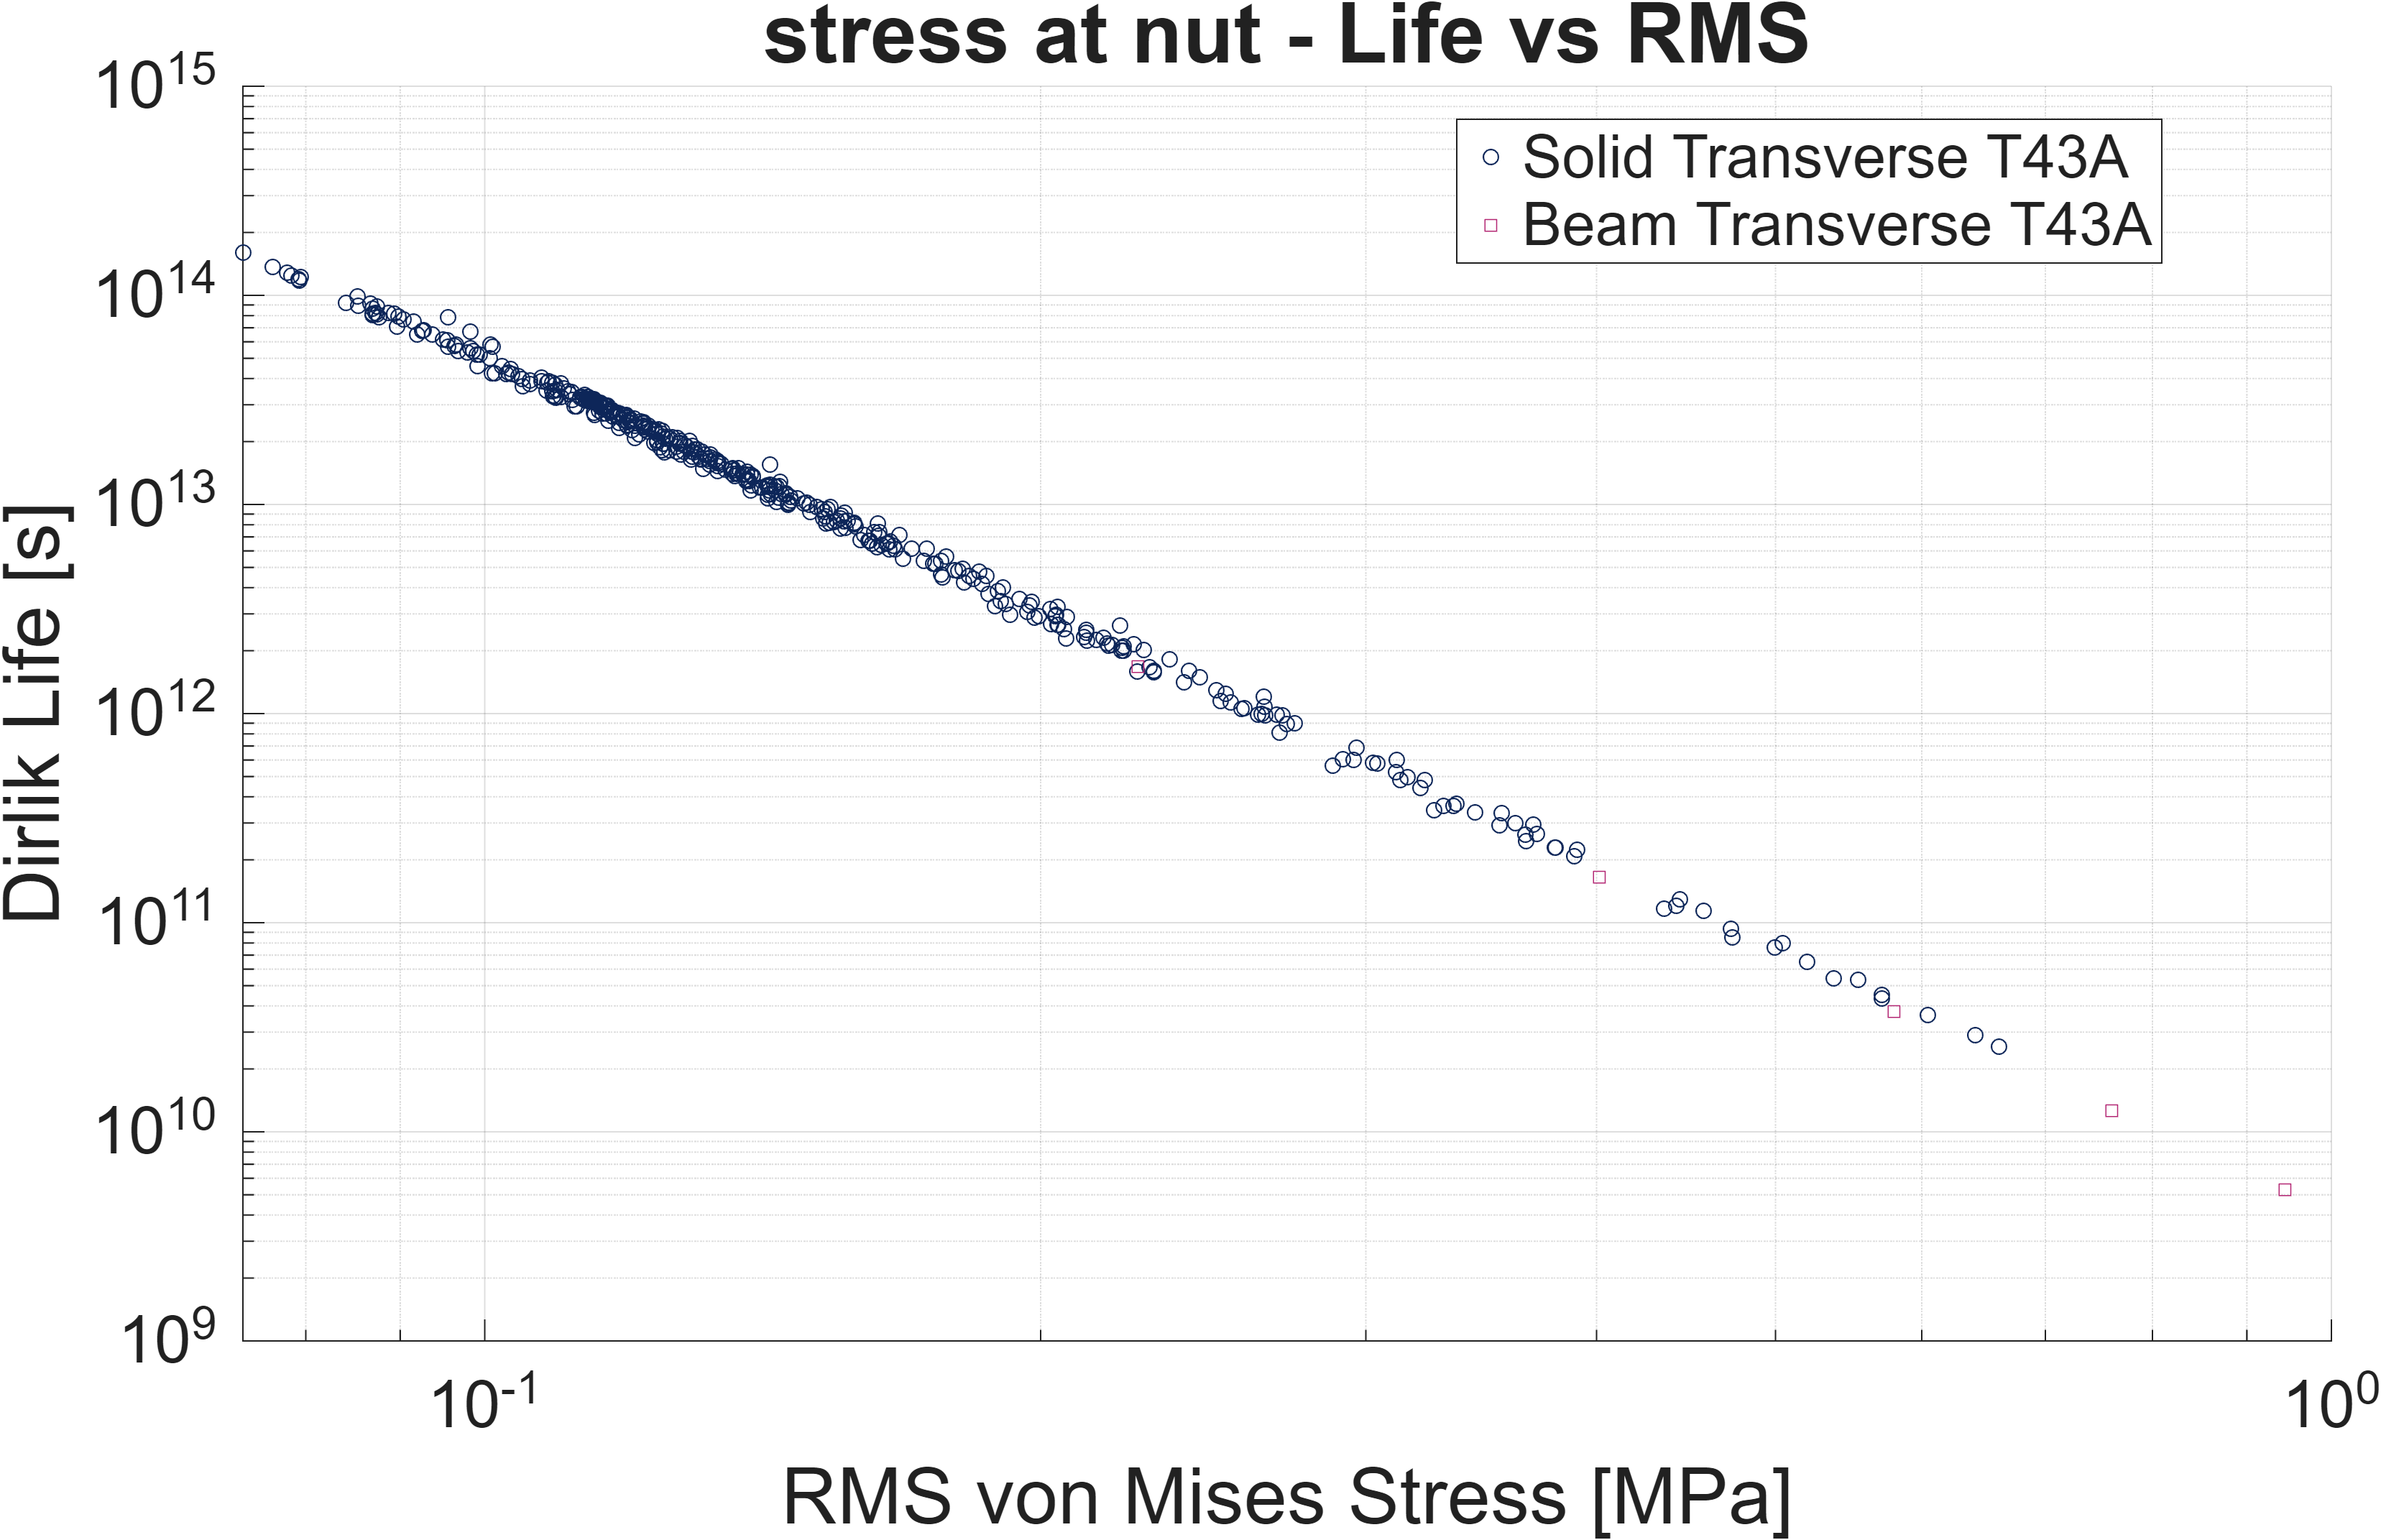
\includegraphics[width=\textwidth]{Transverse T43A/Transverse T43A_life_vs_rms_NODEWISE stress_at_nut.png}
        \caption{Transverse Loading (shear).}
        \label{fig:T43A_shear_life_vs_rms_NODEWISE_stress_at_nut}
    \end{subfigure}
    \begin{subfigure}[b]{0.45\textwidth}
        \centering
        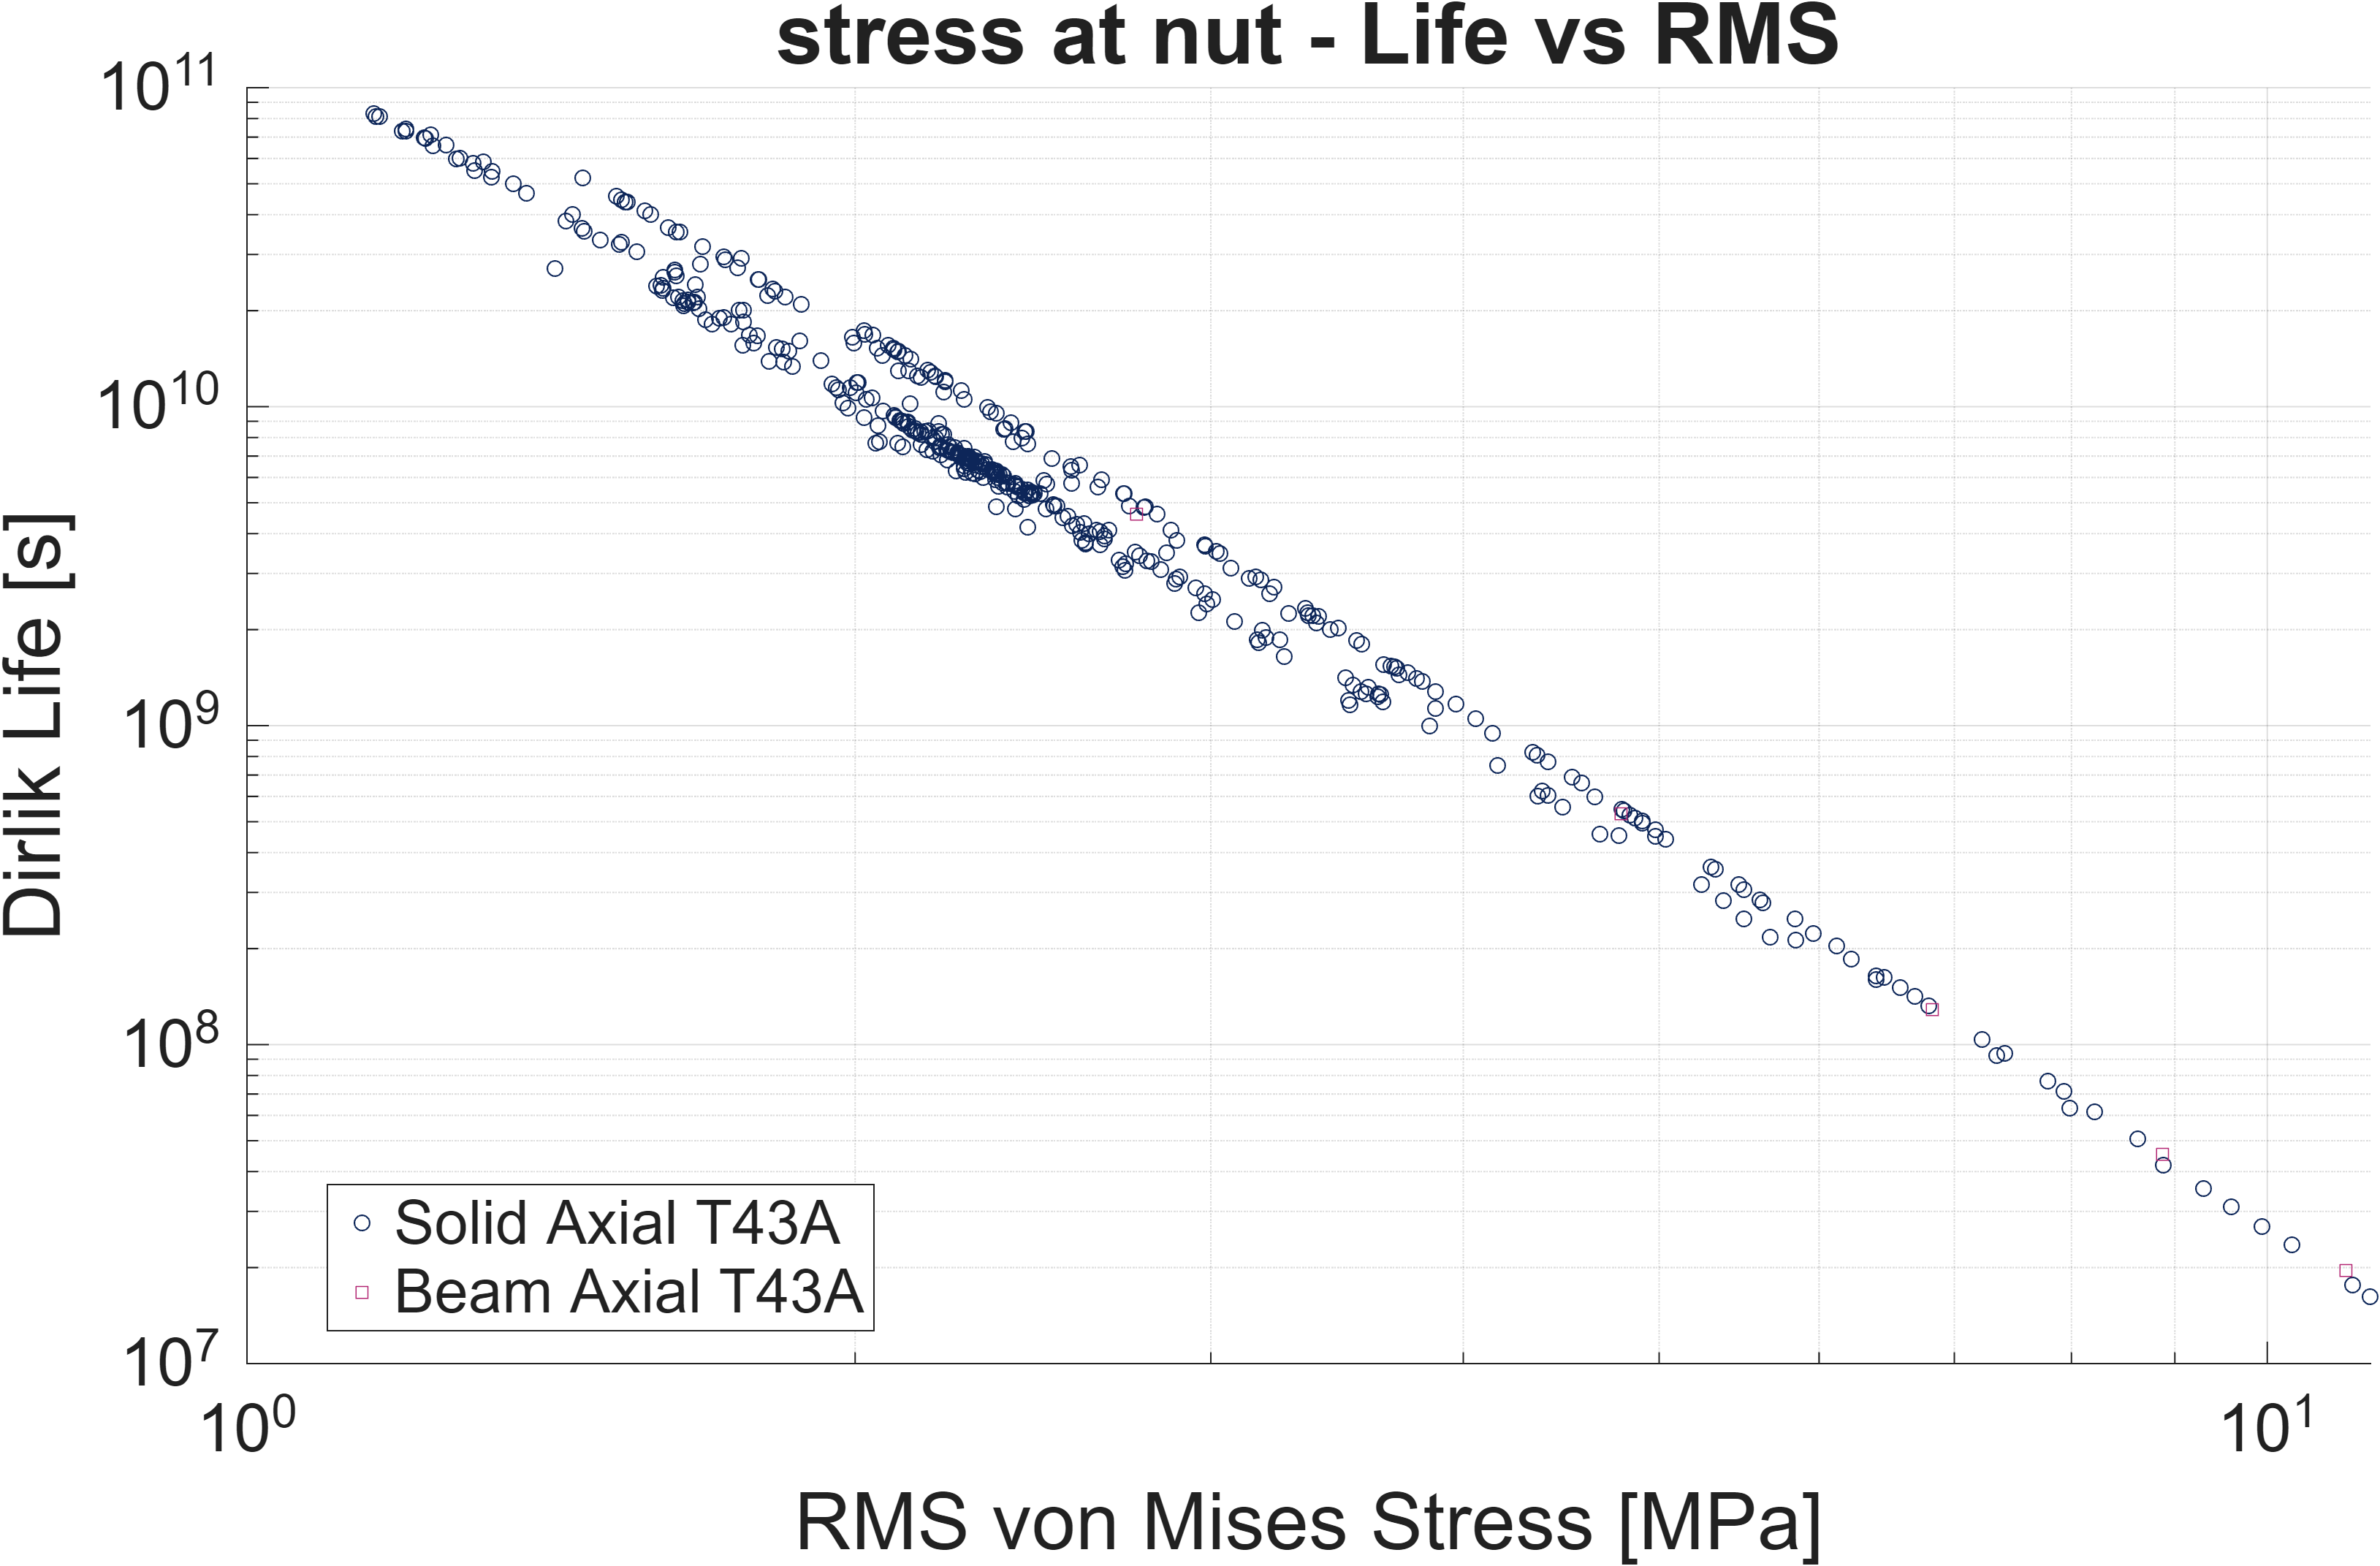
\includegraphics[width=\textwidth]{Axial T43A/Axial T43A_life_vs_rms_NODEWISE stress_at_nut.png}
        \caption{Axial Loading (bending).}
        \label{fig:T43A_bending_life_vs_rms_NODEWISE_stress_at_nut}
    \end{subfigure}
    
    \caption{Dirlik life versus \ac{RMS} stress for the at-nut region, solid model only. Excited by the MIL-STD-810 G profile for the T43A.}
    \label{fig:Life_VS_RMS_atNut_T43A}
\end{figure}

\begin{figure}[H]
    \centering
    \begin{subfigure}[b]{0.45\textwidth}
        \centering
        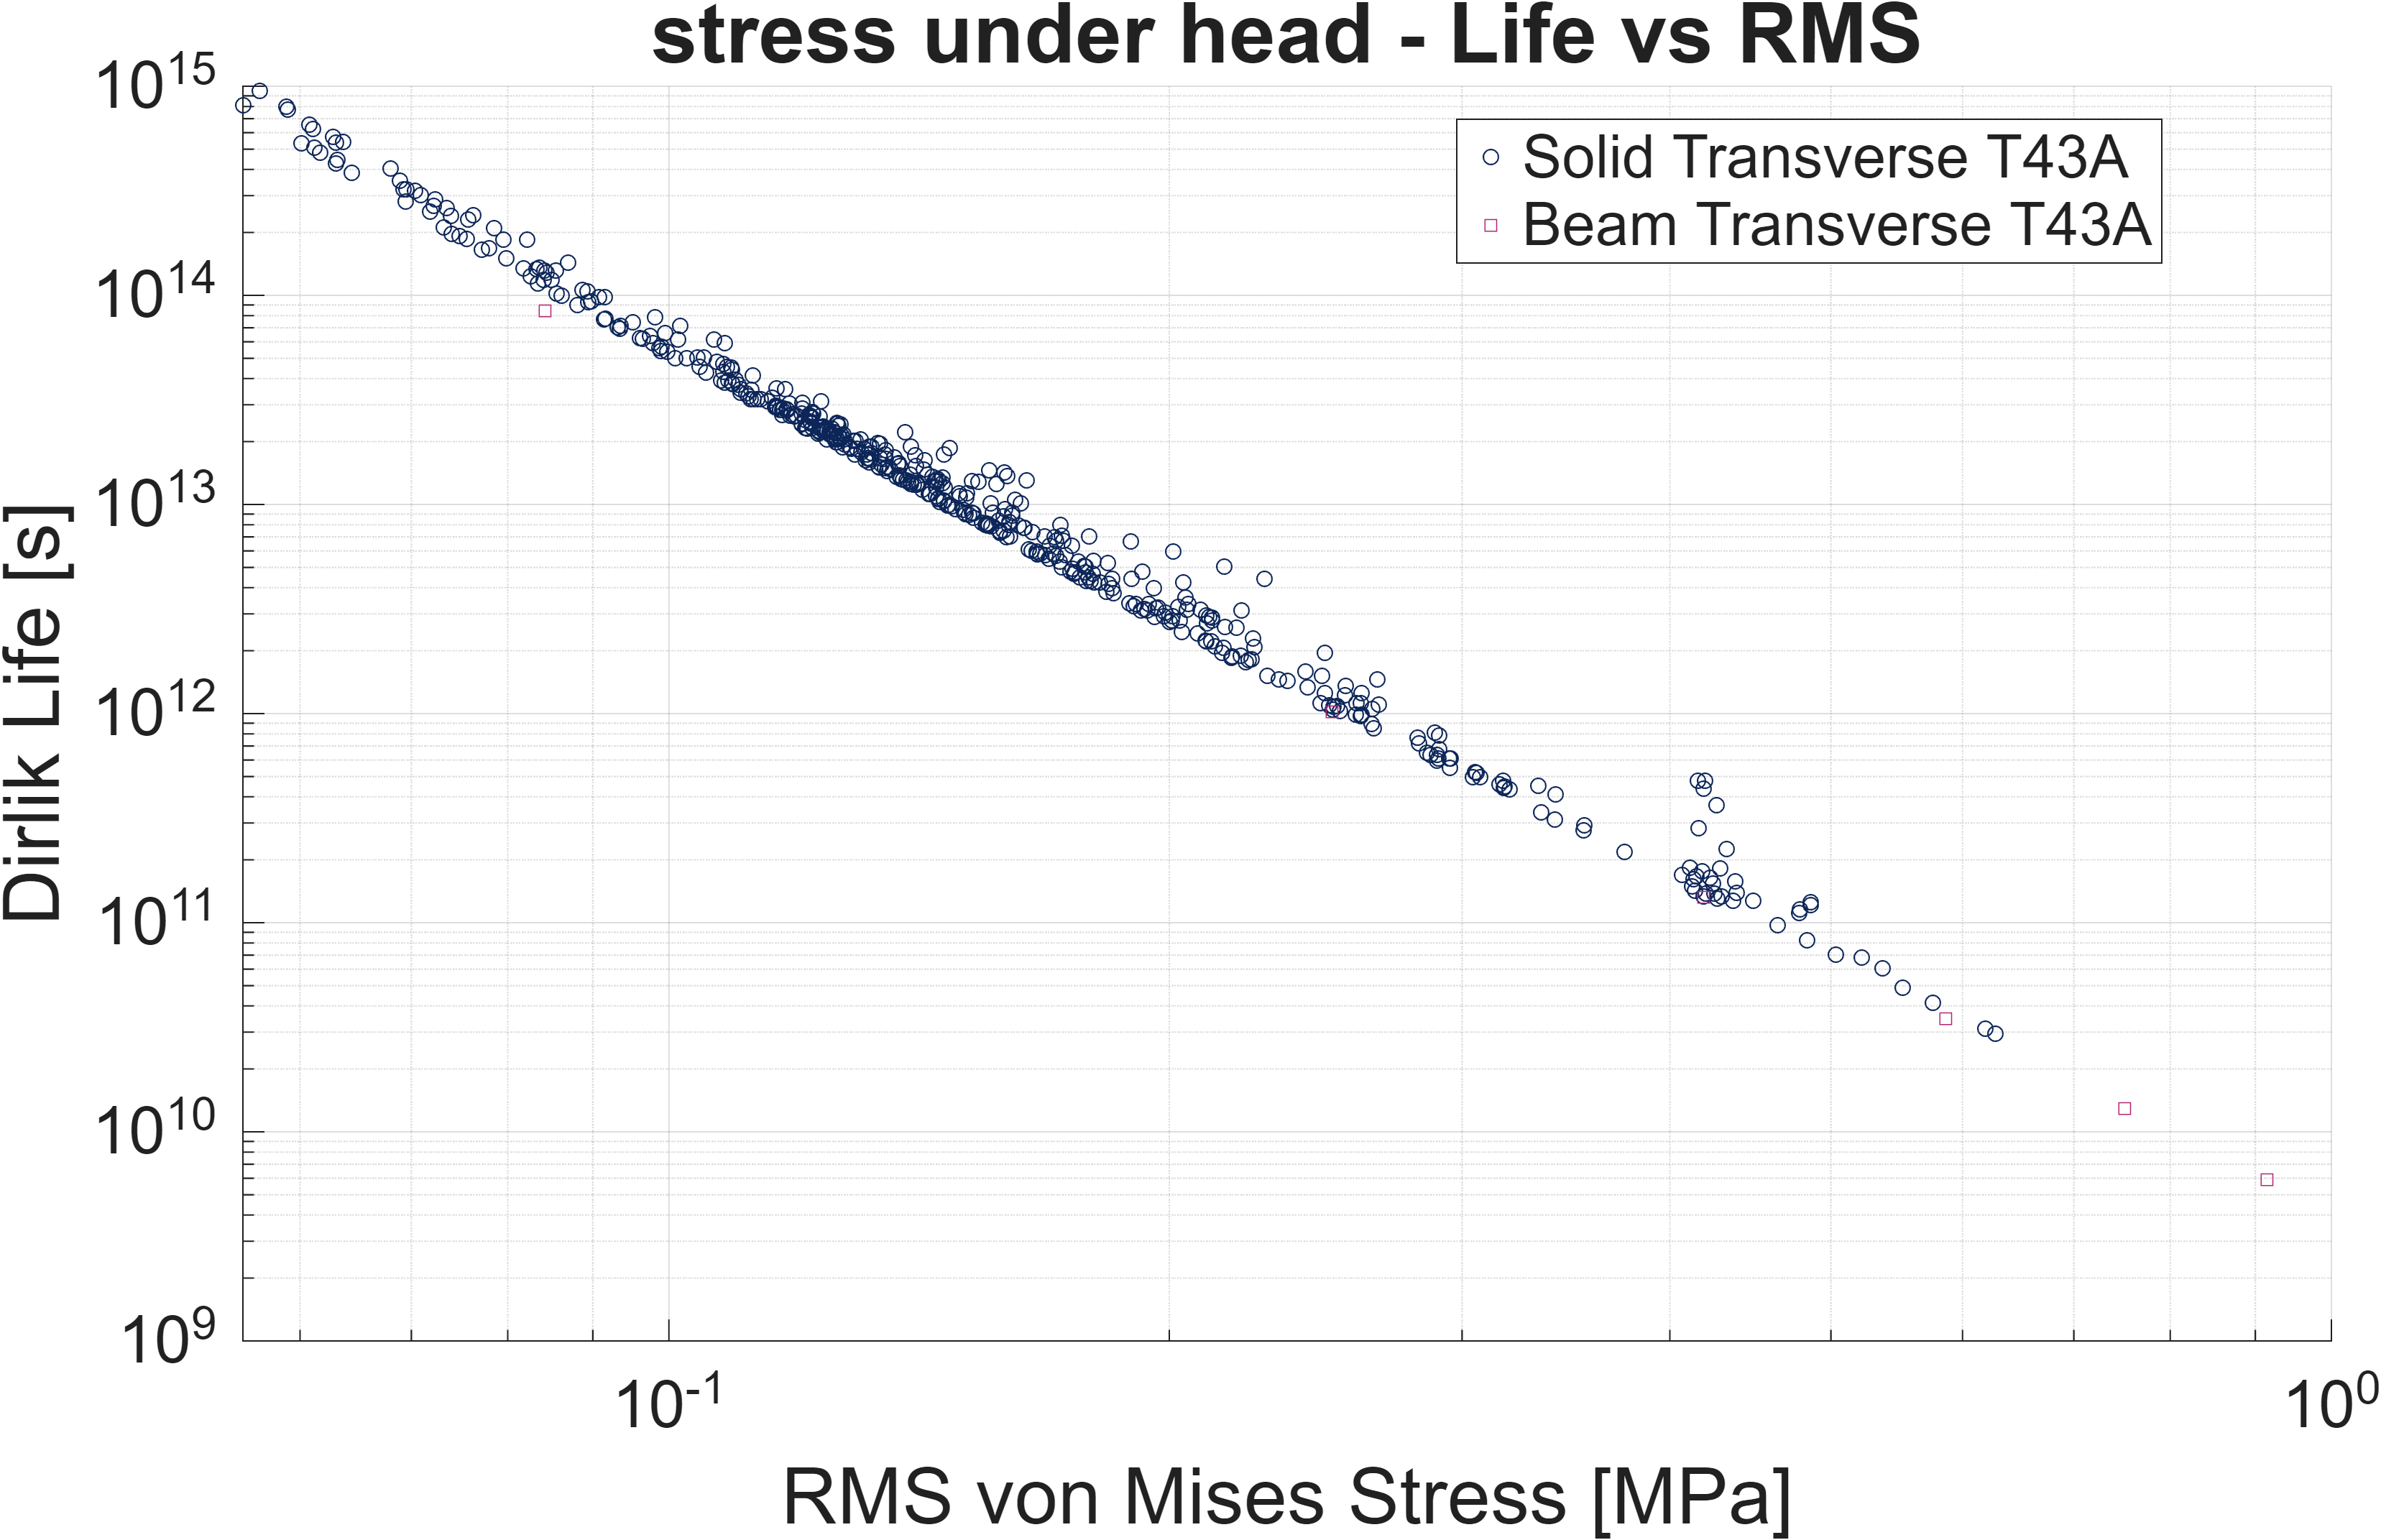
\includegraphics[width=\textwidth]{Transverse T43A/Transverse T43A_life_vs_rms_NODEWISE stress_under_head.png}
        \caption{Transverse Loading (shear).}
        \label{fig:T43A_shear_life_vs_rms_NODEWISE_stress_under_head}
    \end{subfigure}
    \begin{subfigure}[b]{0.45\textwidth}
        \centering
        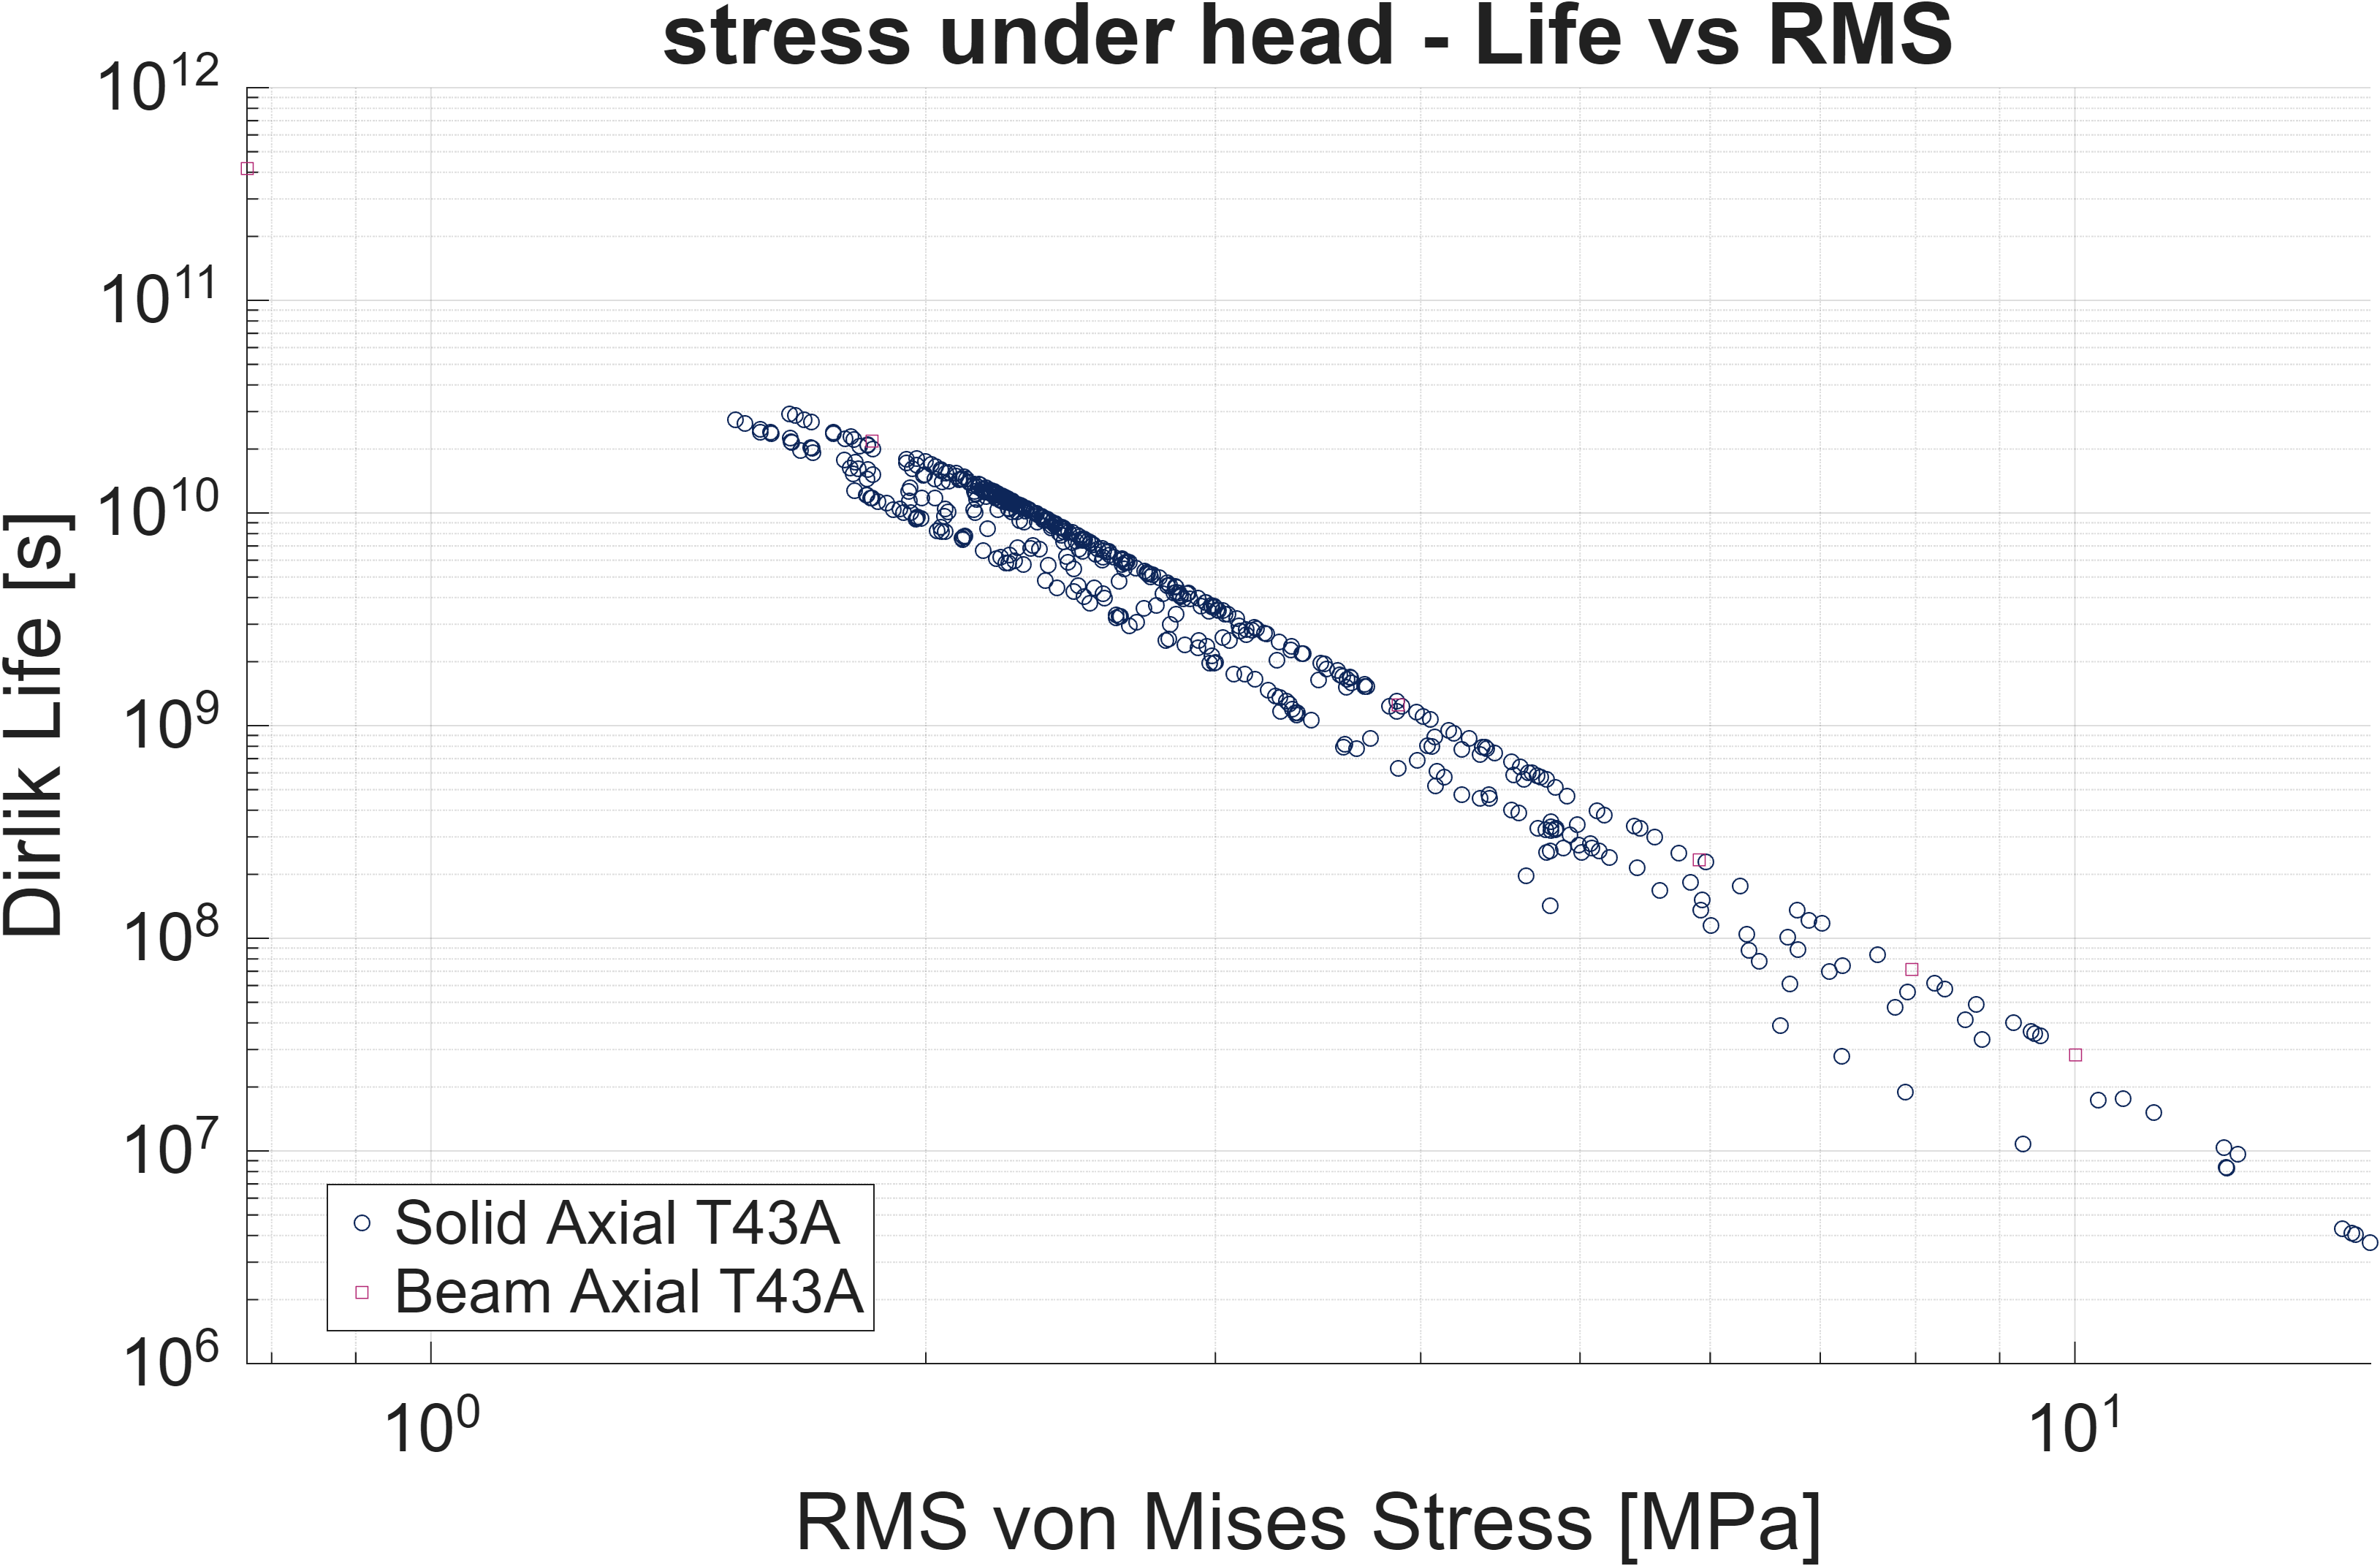
\includegraphics[width=\textwidth]{Axial T43A/Axial T43A_life_vs_rms_NODEWISE stress_under_head.png}
        \caption{Axial Loading (bending).}
        \label{fig:T43A_bending_life_vs_rms_NODEWISE_stress_under_head}
    \end{subfigure}
    
    \caption{Dirlik life versus \ac{RMS} stress for the under-head region, solid model only. Excited by the MIL-STD 810G profile for T43A.}
    \label{fig:Life_VS_RMS_underHead_T43A}
\end{figure}

\begin{figure}[H]
    \centering
    \begin{subfigure}[b]{0.45\textwidth}
        \centering
        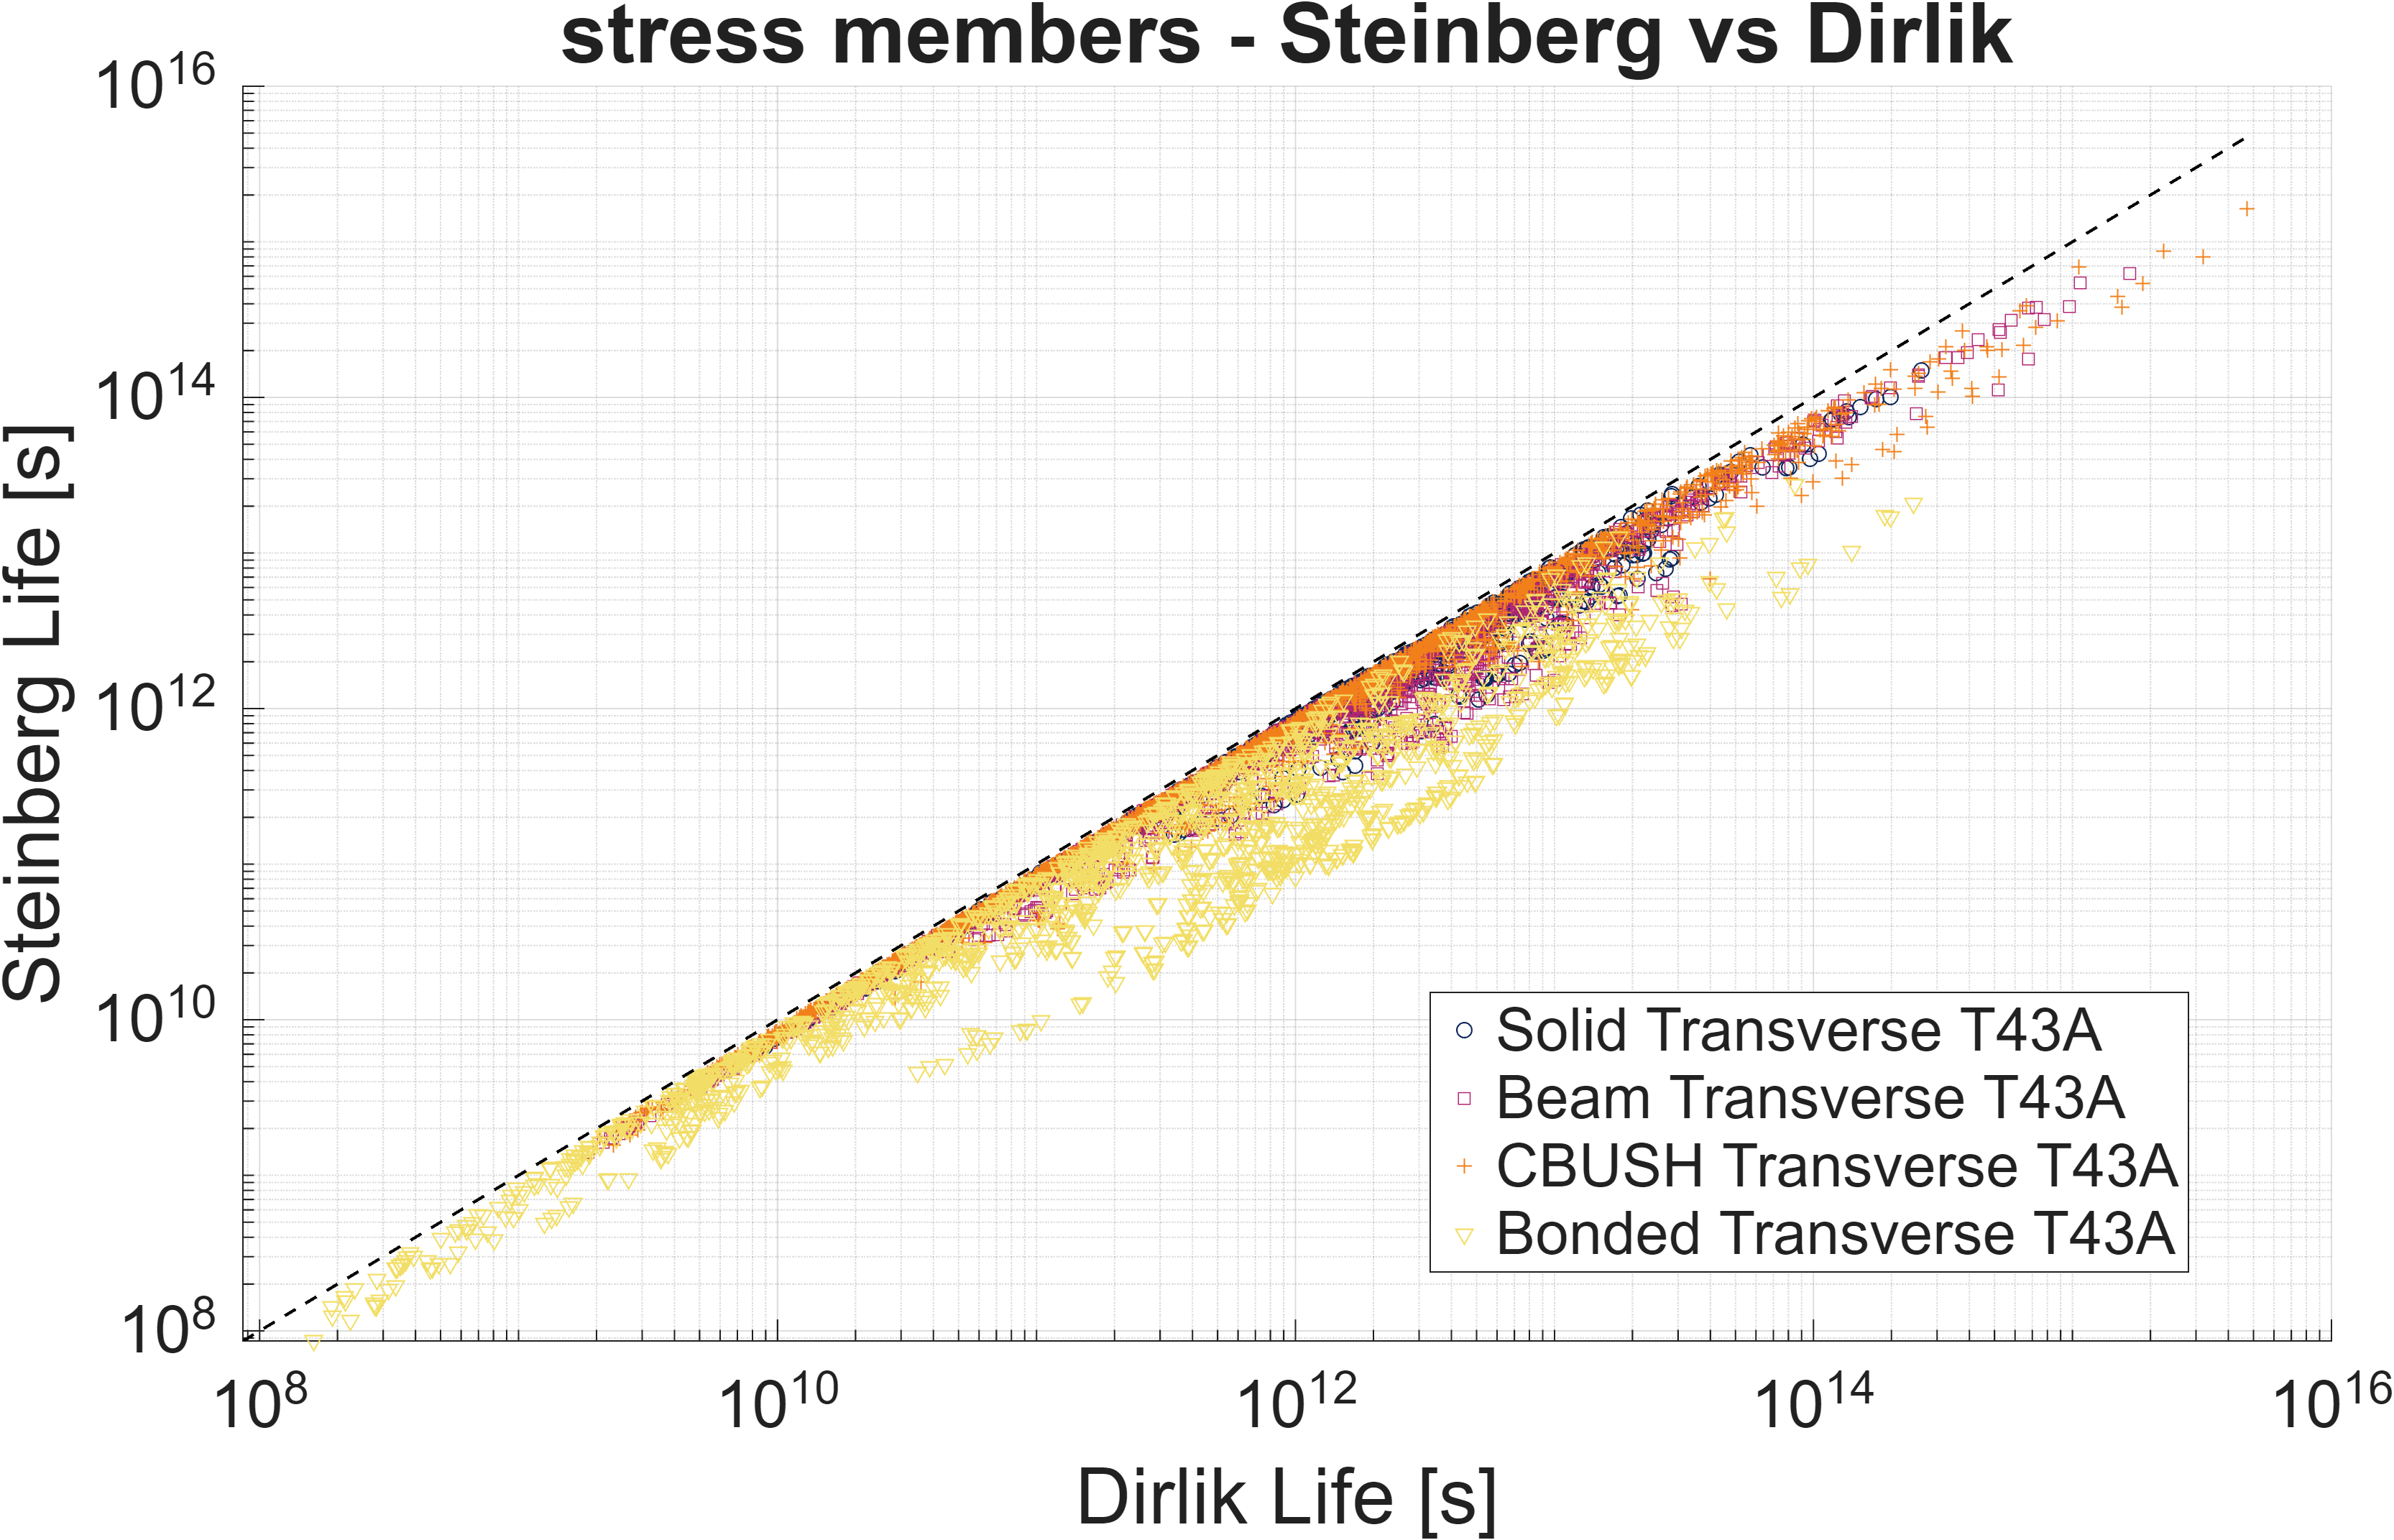
\includegraphics[width=\textwidth]{Transverse T43A/Transverse T43A_steinberg_vs_dirlik_NODEWISE stress_members.png}
        \caption{Transverse Loading (shear).}
        \label{fig:T43A_shear_steinberg_vs_dirlik_NODEWISE_stress_members}
    \end{subfigure}
    \begin{subfigure}[b]{0.45\textwidth}
        \centering
        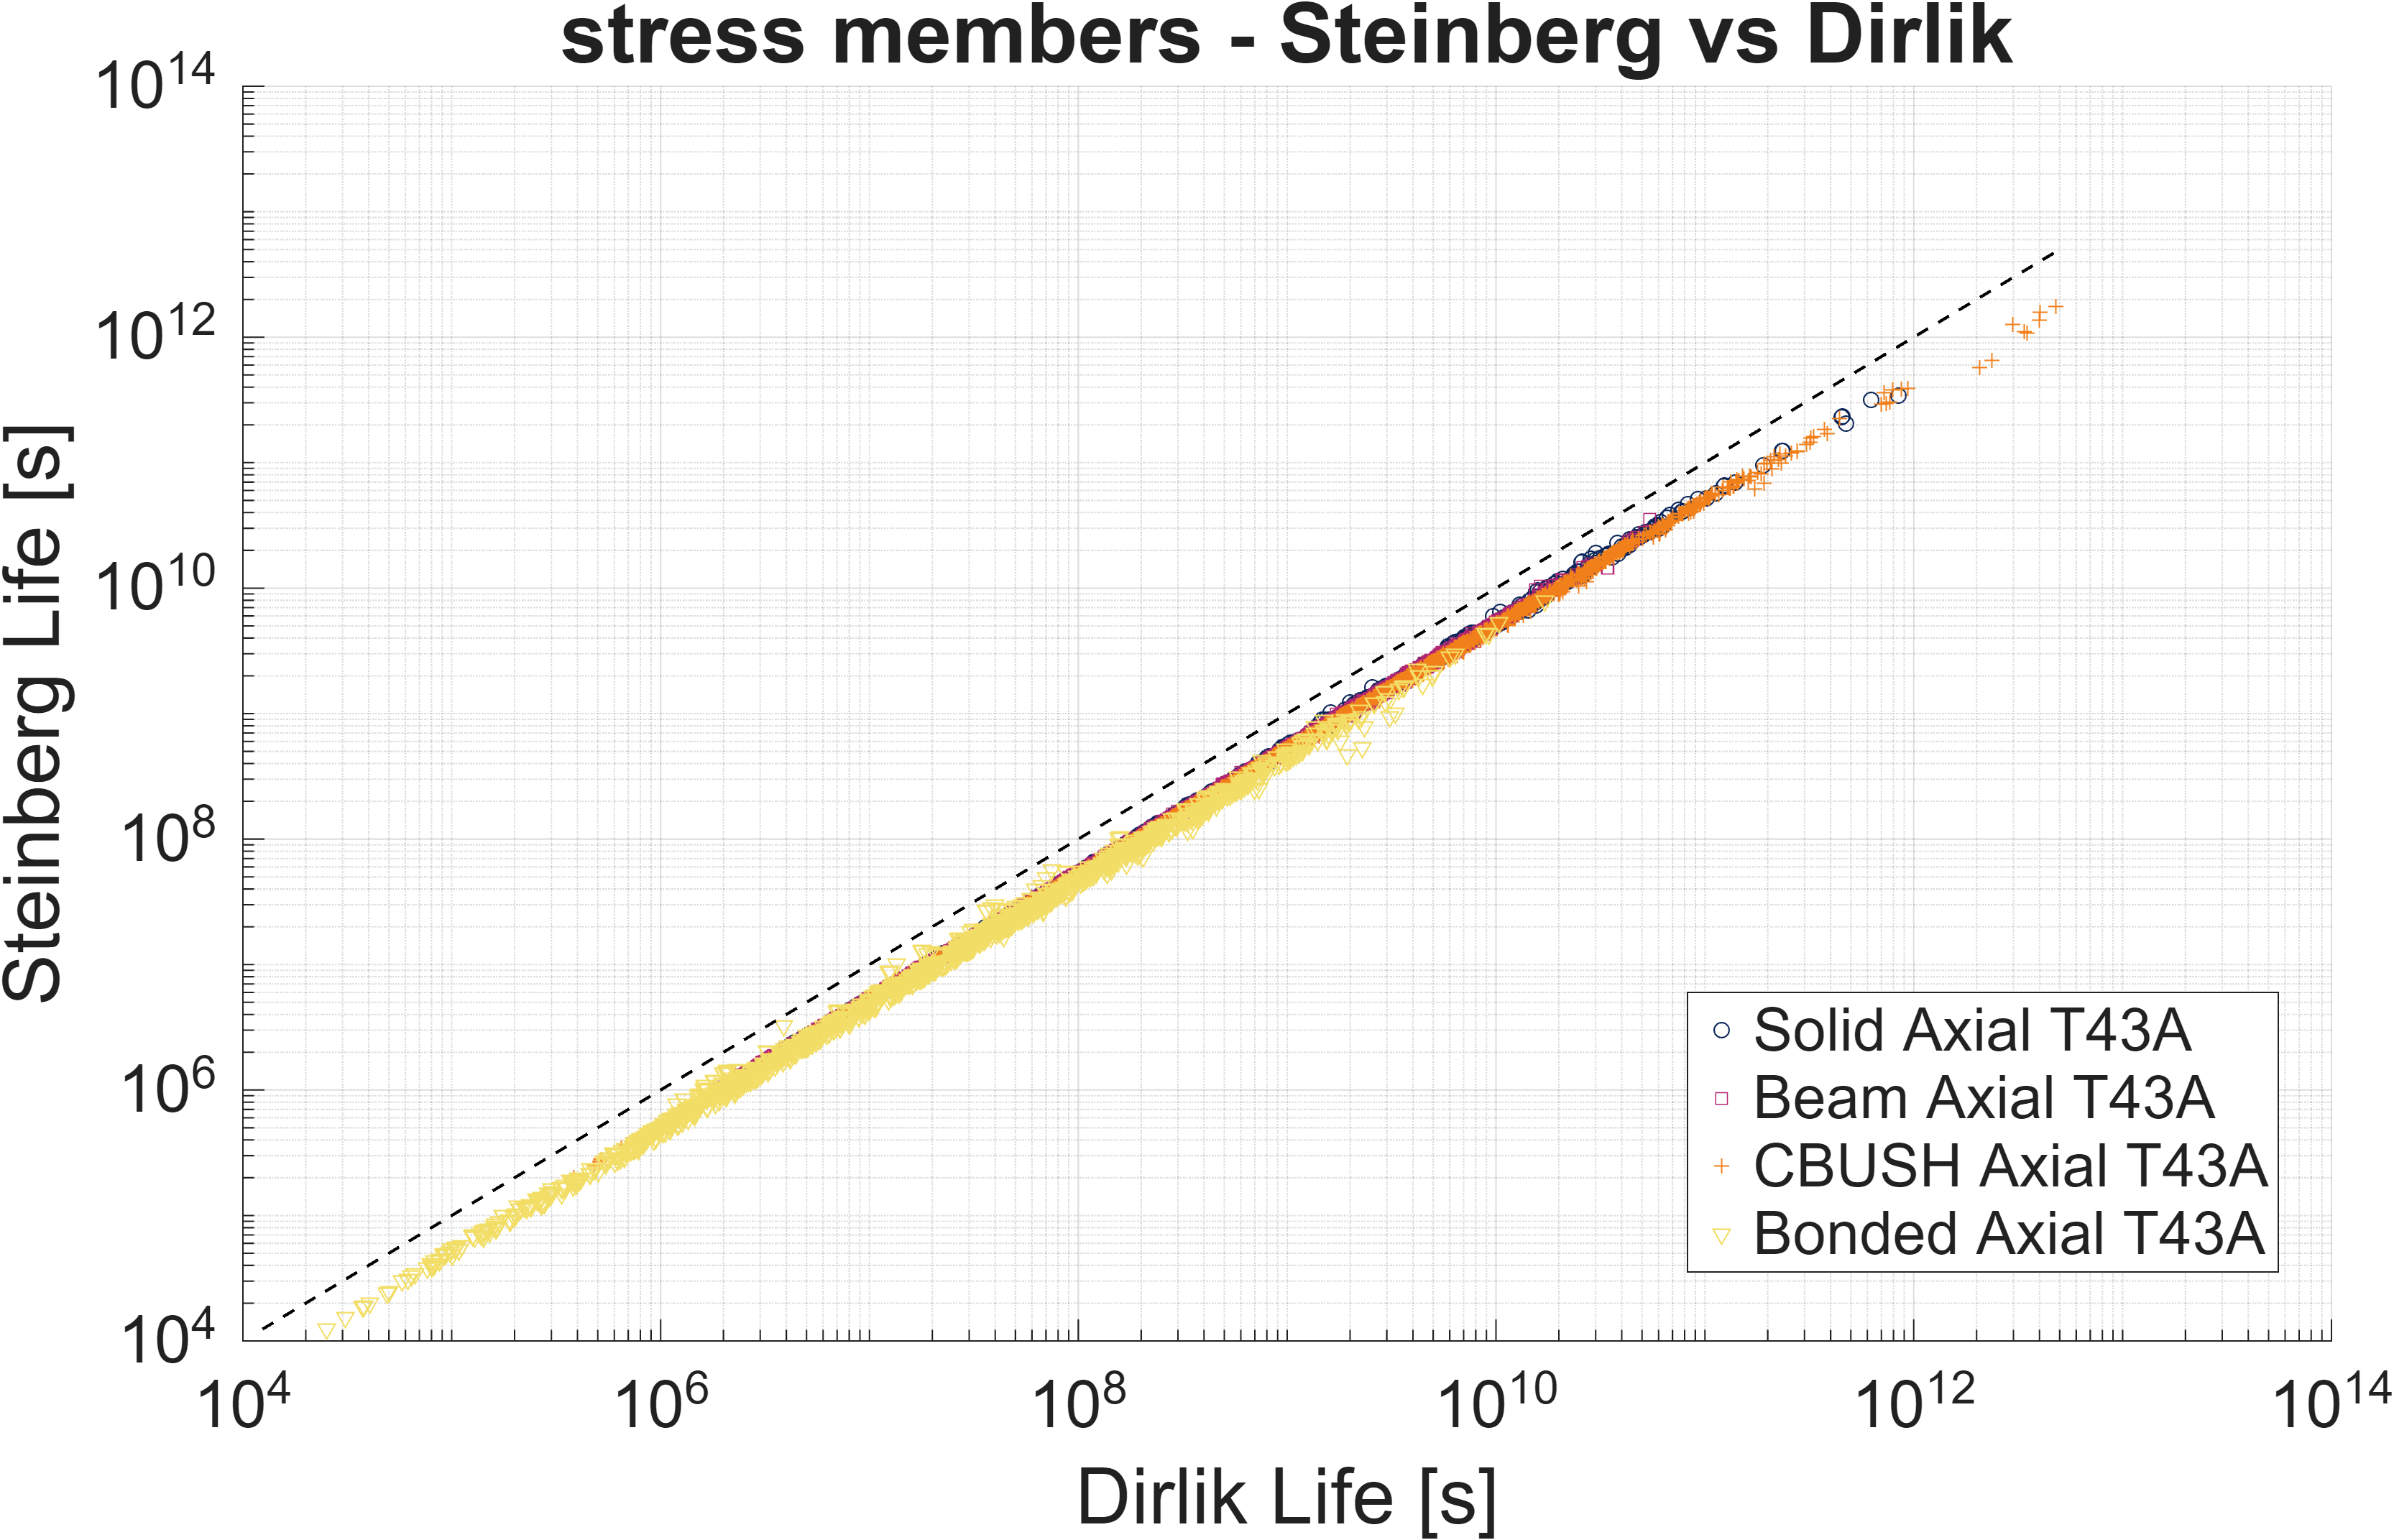
\includegraphics[width=\textwidth]{Axial T43A/Axial T43A_steinberg_vs_dirlik_NODEWISE stress_members.png}
        \caption{Axial Loading (bending).}
        \label{fig:T43A_bending_steinberg_vs_dirlik_NODEWISE_stress_members}
    \end{subfigure}
    
    \caption{Steinberg versus Dirlik fatigue life for the clamped members region. At short lives, the two methods agree closely, but at long lives (low-stress nodes), Steinberg tends to underpredict relative to Dirlik. Excited by the MIL-STD 810G profile for T43A.}
    \label{fig:SteinbergDirlik_members_T43A}
\end{figure}

\begin{figure}[H]
    \centering
    \begin{subfigure}[b]{0.45\textwidth}
        \centering
        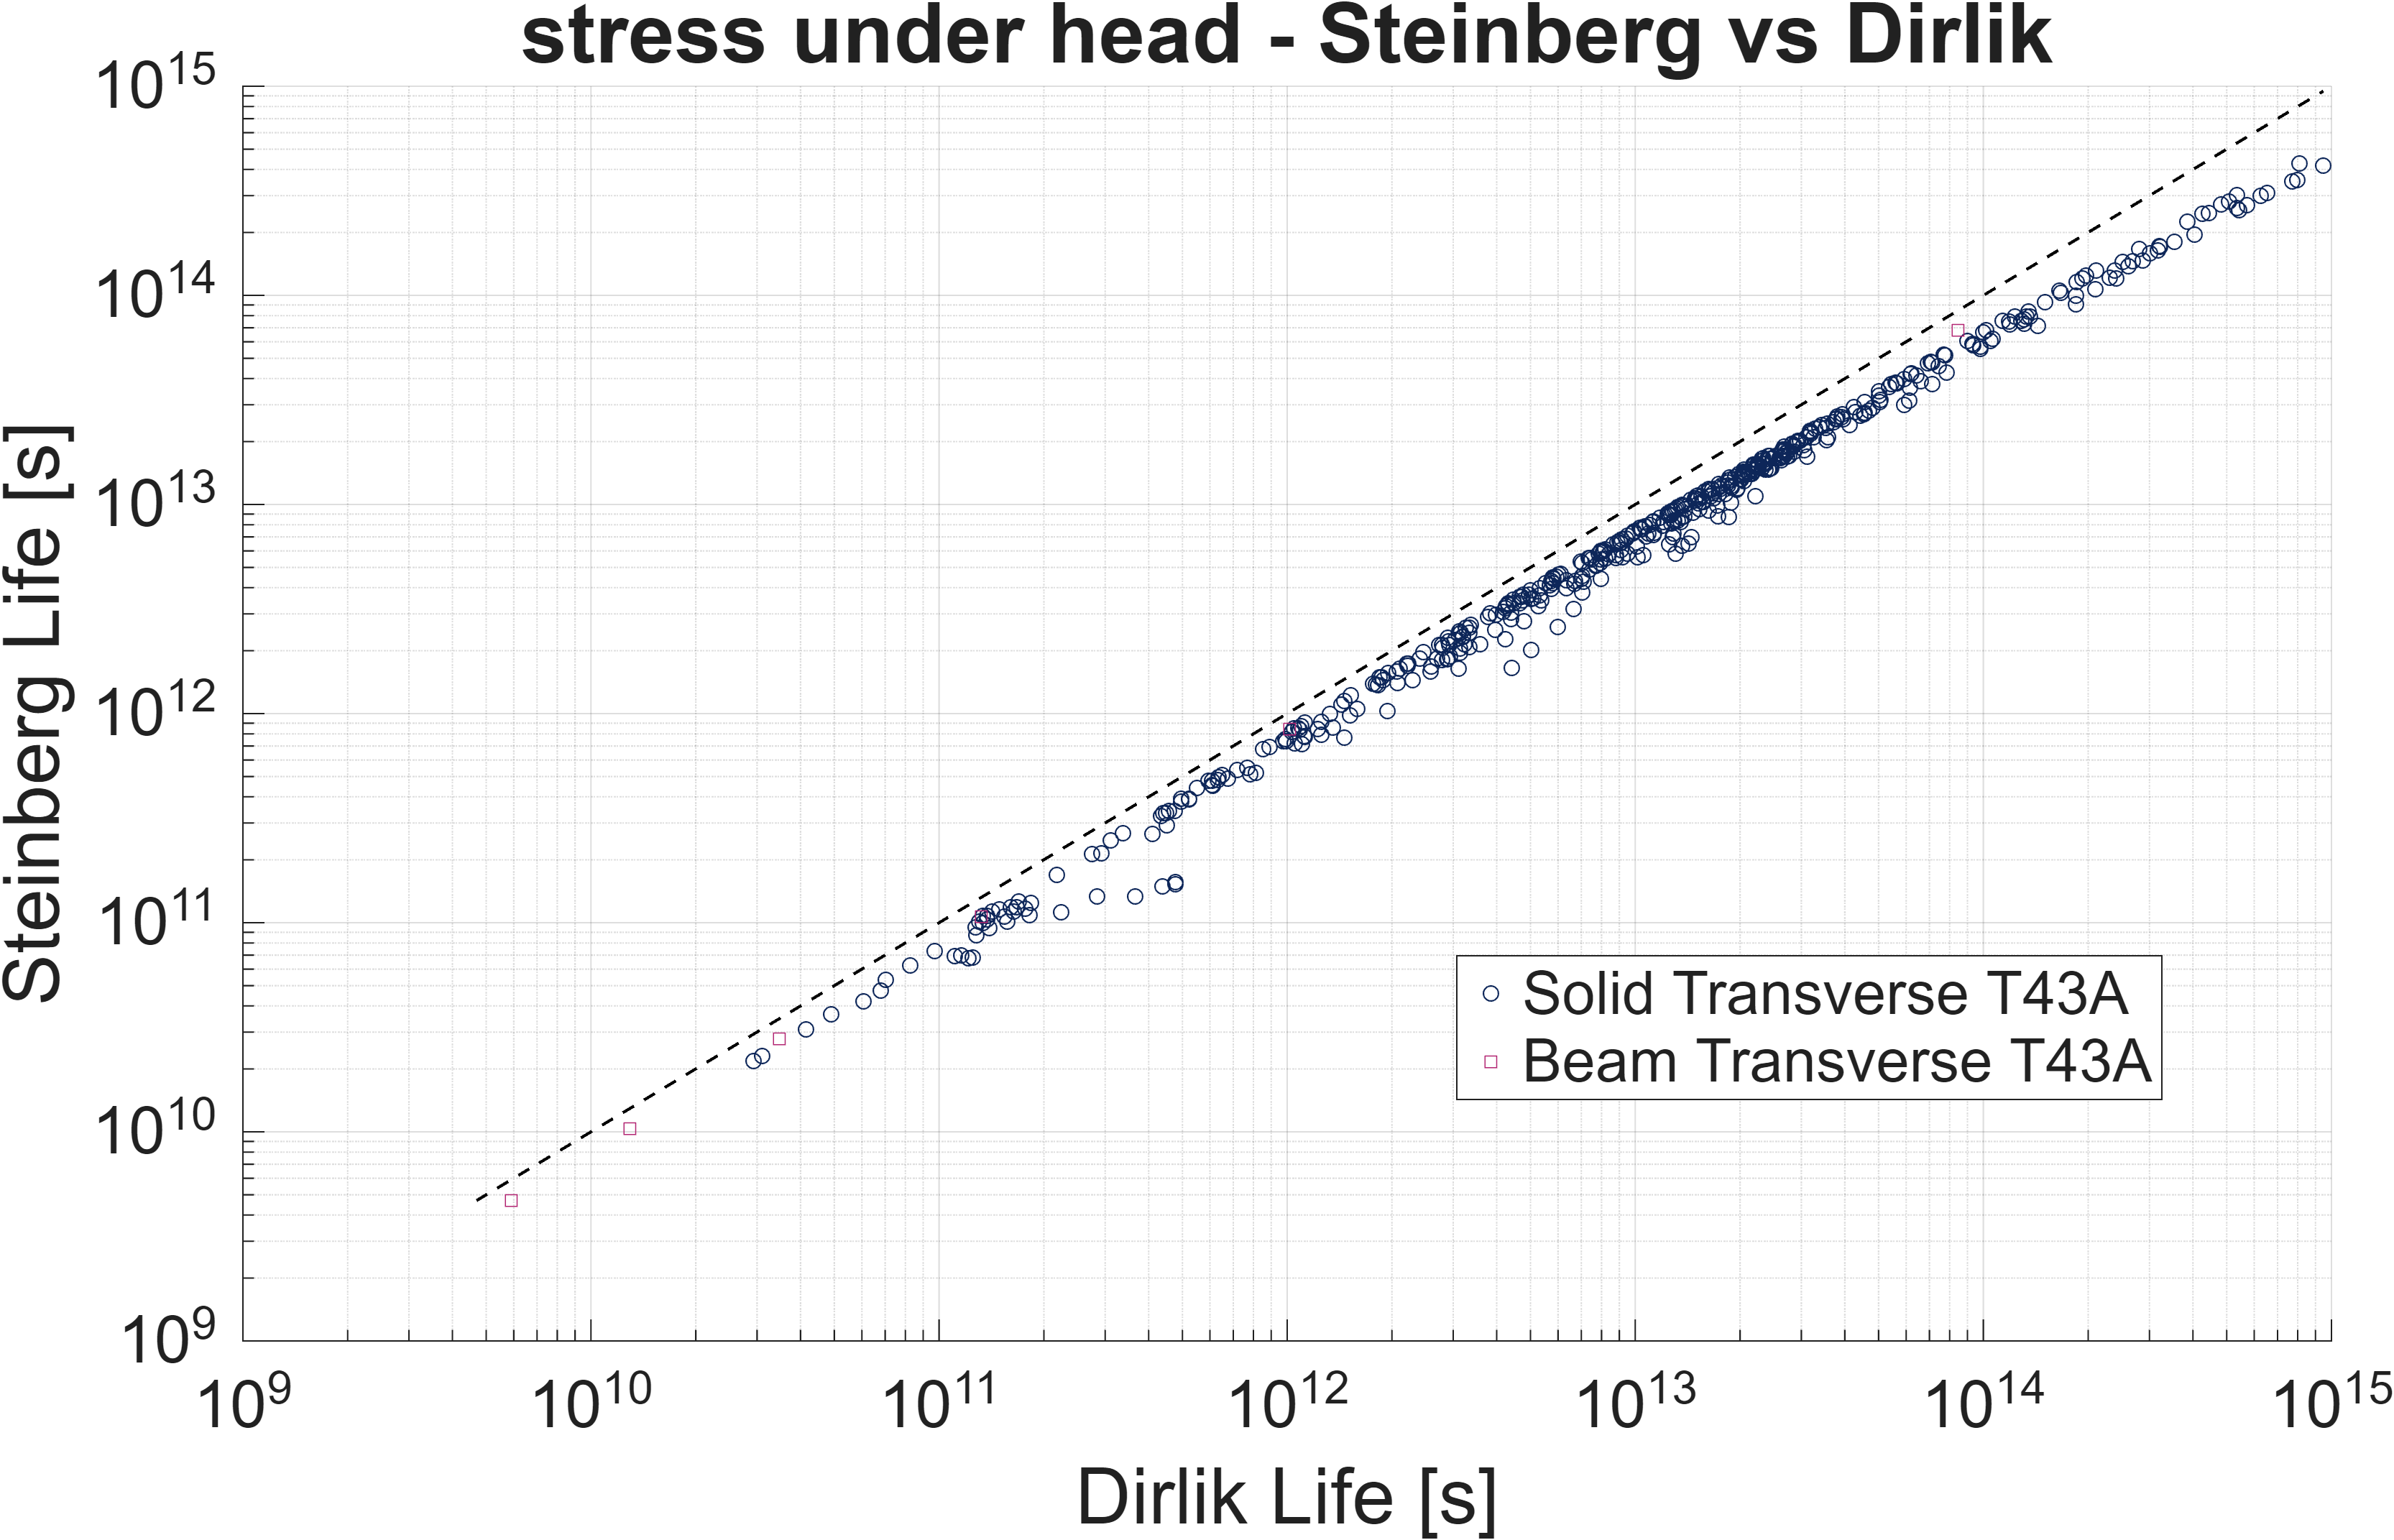
\includegraphics[width=\textwidth]{Transverse T43A/Transverse T43A_steinberg_vs_dirlik_NODEWISE stress_under_head.png}
        \caption{Transverse Loading (shear).}
        \label{fig:T43A_shear_steinberg_vs_dirlik_NODEWISE_stress_under_head}
    \end{subfigure}
    \begin{subfigure}[b]{0.45\textwidth}
        \centering
        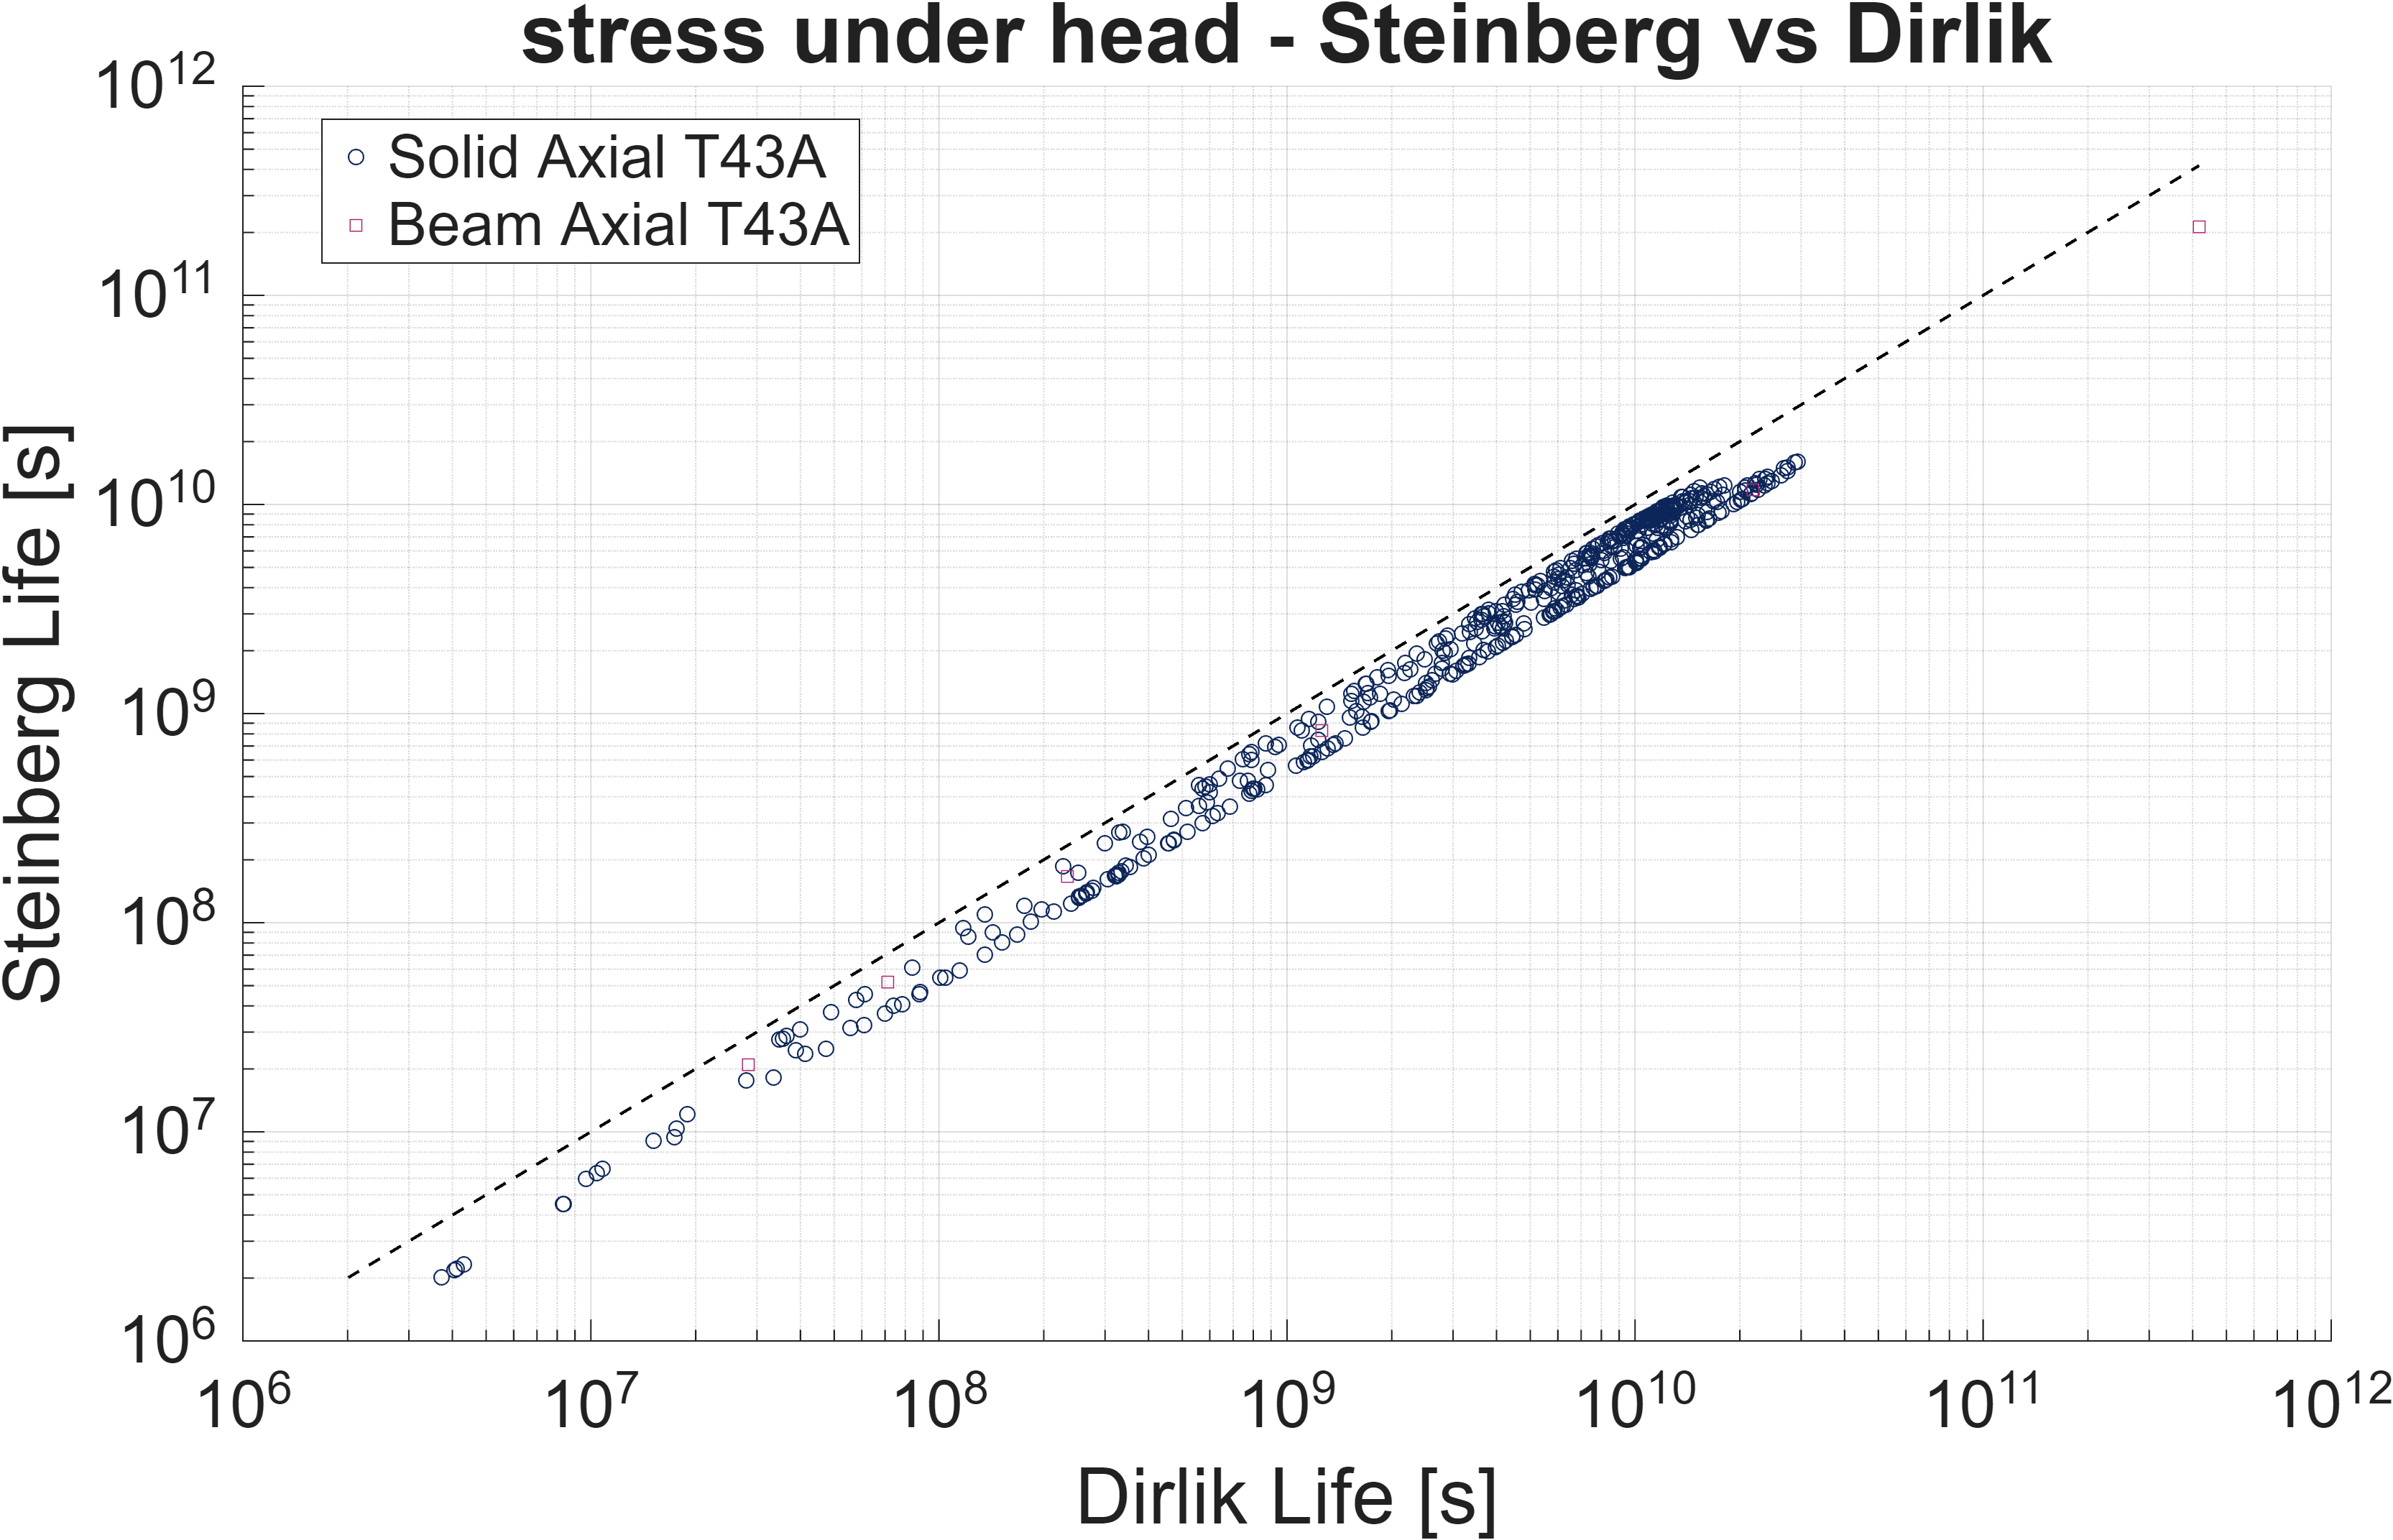
\includegraphics[width=\textwidth]{Axial T43A/Axial T43A_steinberg_vs_dirlik_NODEWISE stress_under_head.png}
        \caption{Axial Loading (bending).}
        \label{fig:T43A_bending_steinberg_vs_dirlik_NODEWISE_stress_under_head}
    \end{subfigure}
    
    \caption{Steinberg versus Dirlik fatigue life for the under-head region (solid model only). Excited by the MIL-STD 810G profile for T43A.}
    \label{fig:SteinbergDirlik_underHead_T43A}
\end{figure}

\begin{figure}[H]
    \centering
    \begin{subfigure}[b]{0.45\textwidth}
        \centering
        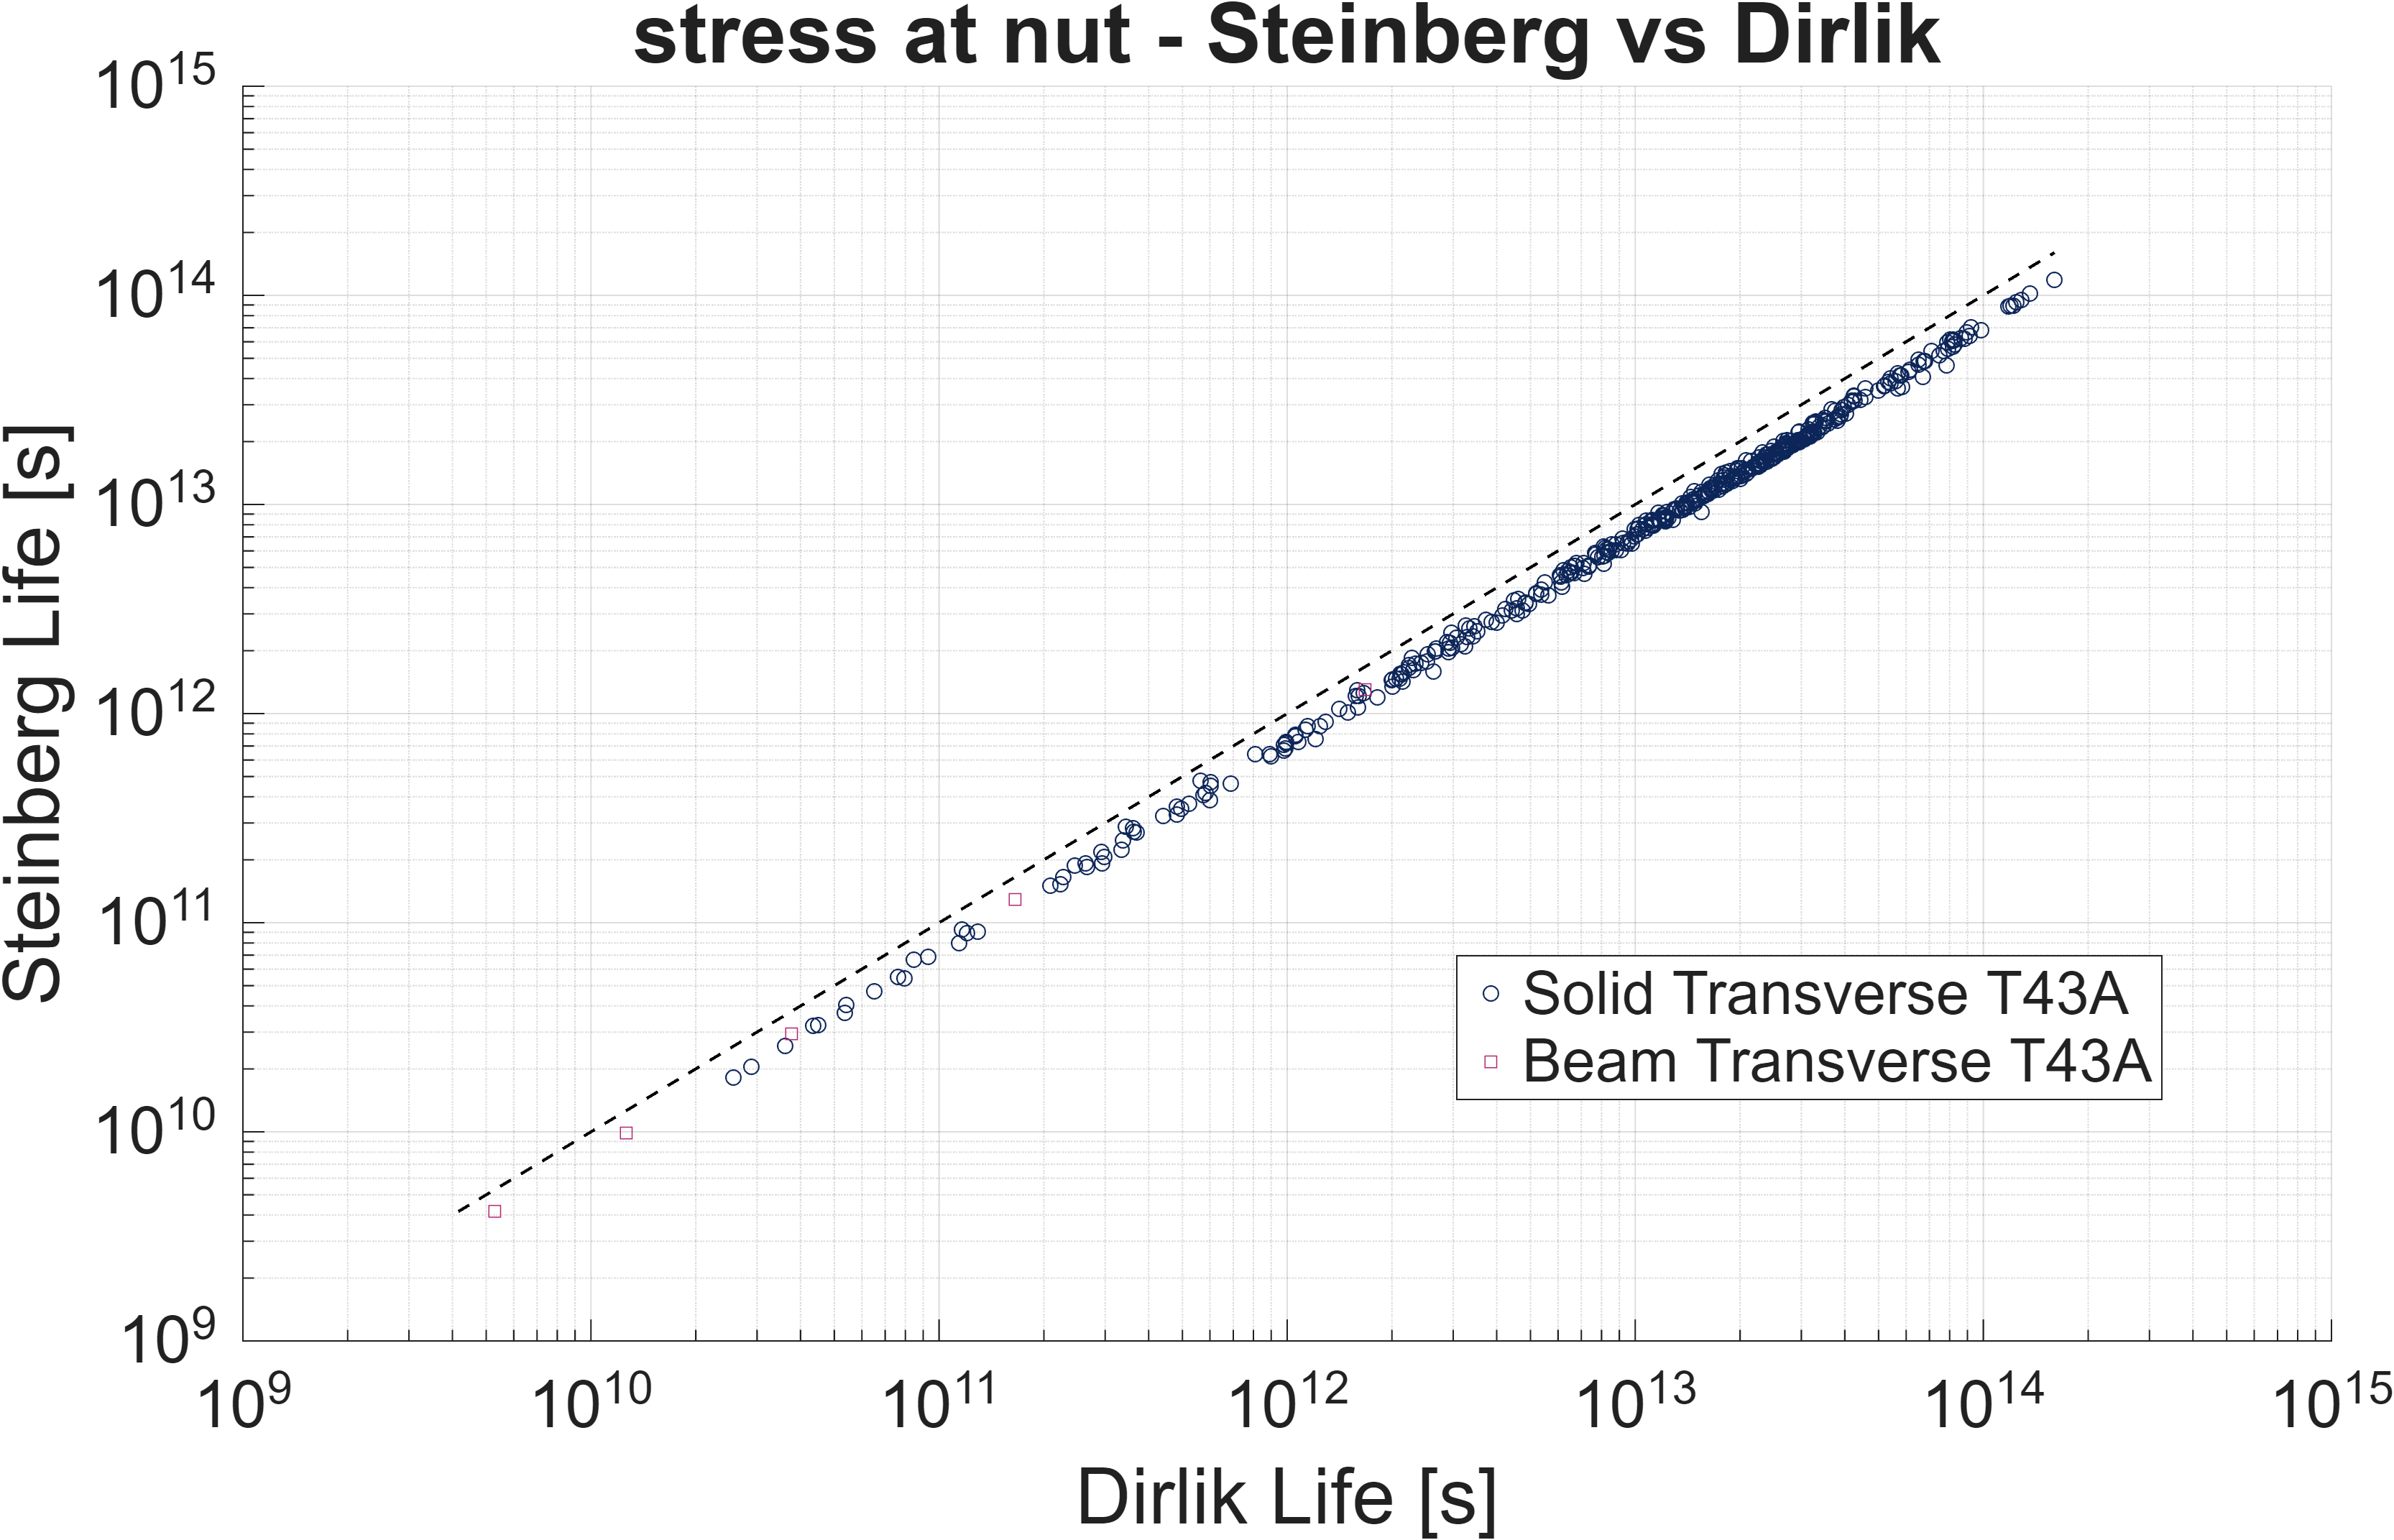
\includegraphics[width=\textwidth]{Transverse T43A/Transverse T43A_steinberg_vs_dirlik_NODEWISE stress_at_nut.png}
        \caption{Transverse Loading (shear).}
        \label{fig:T43A_shear_steinberg_vs_dirlik_NODEWISE_stress_at_nut}
    \end{subfigure}
    \begin{subfigure}[b]{0.45\textwidth}
        \centering
        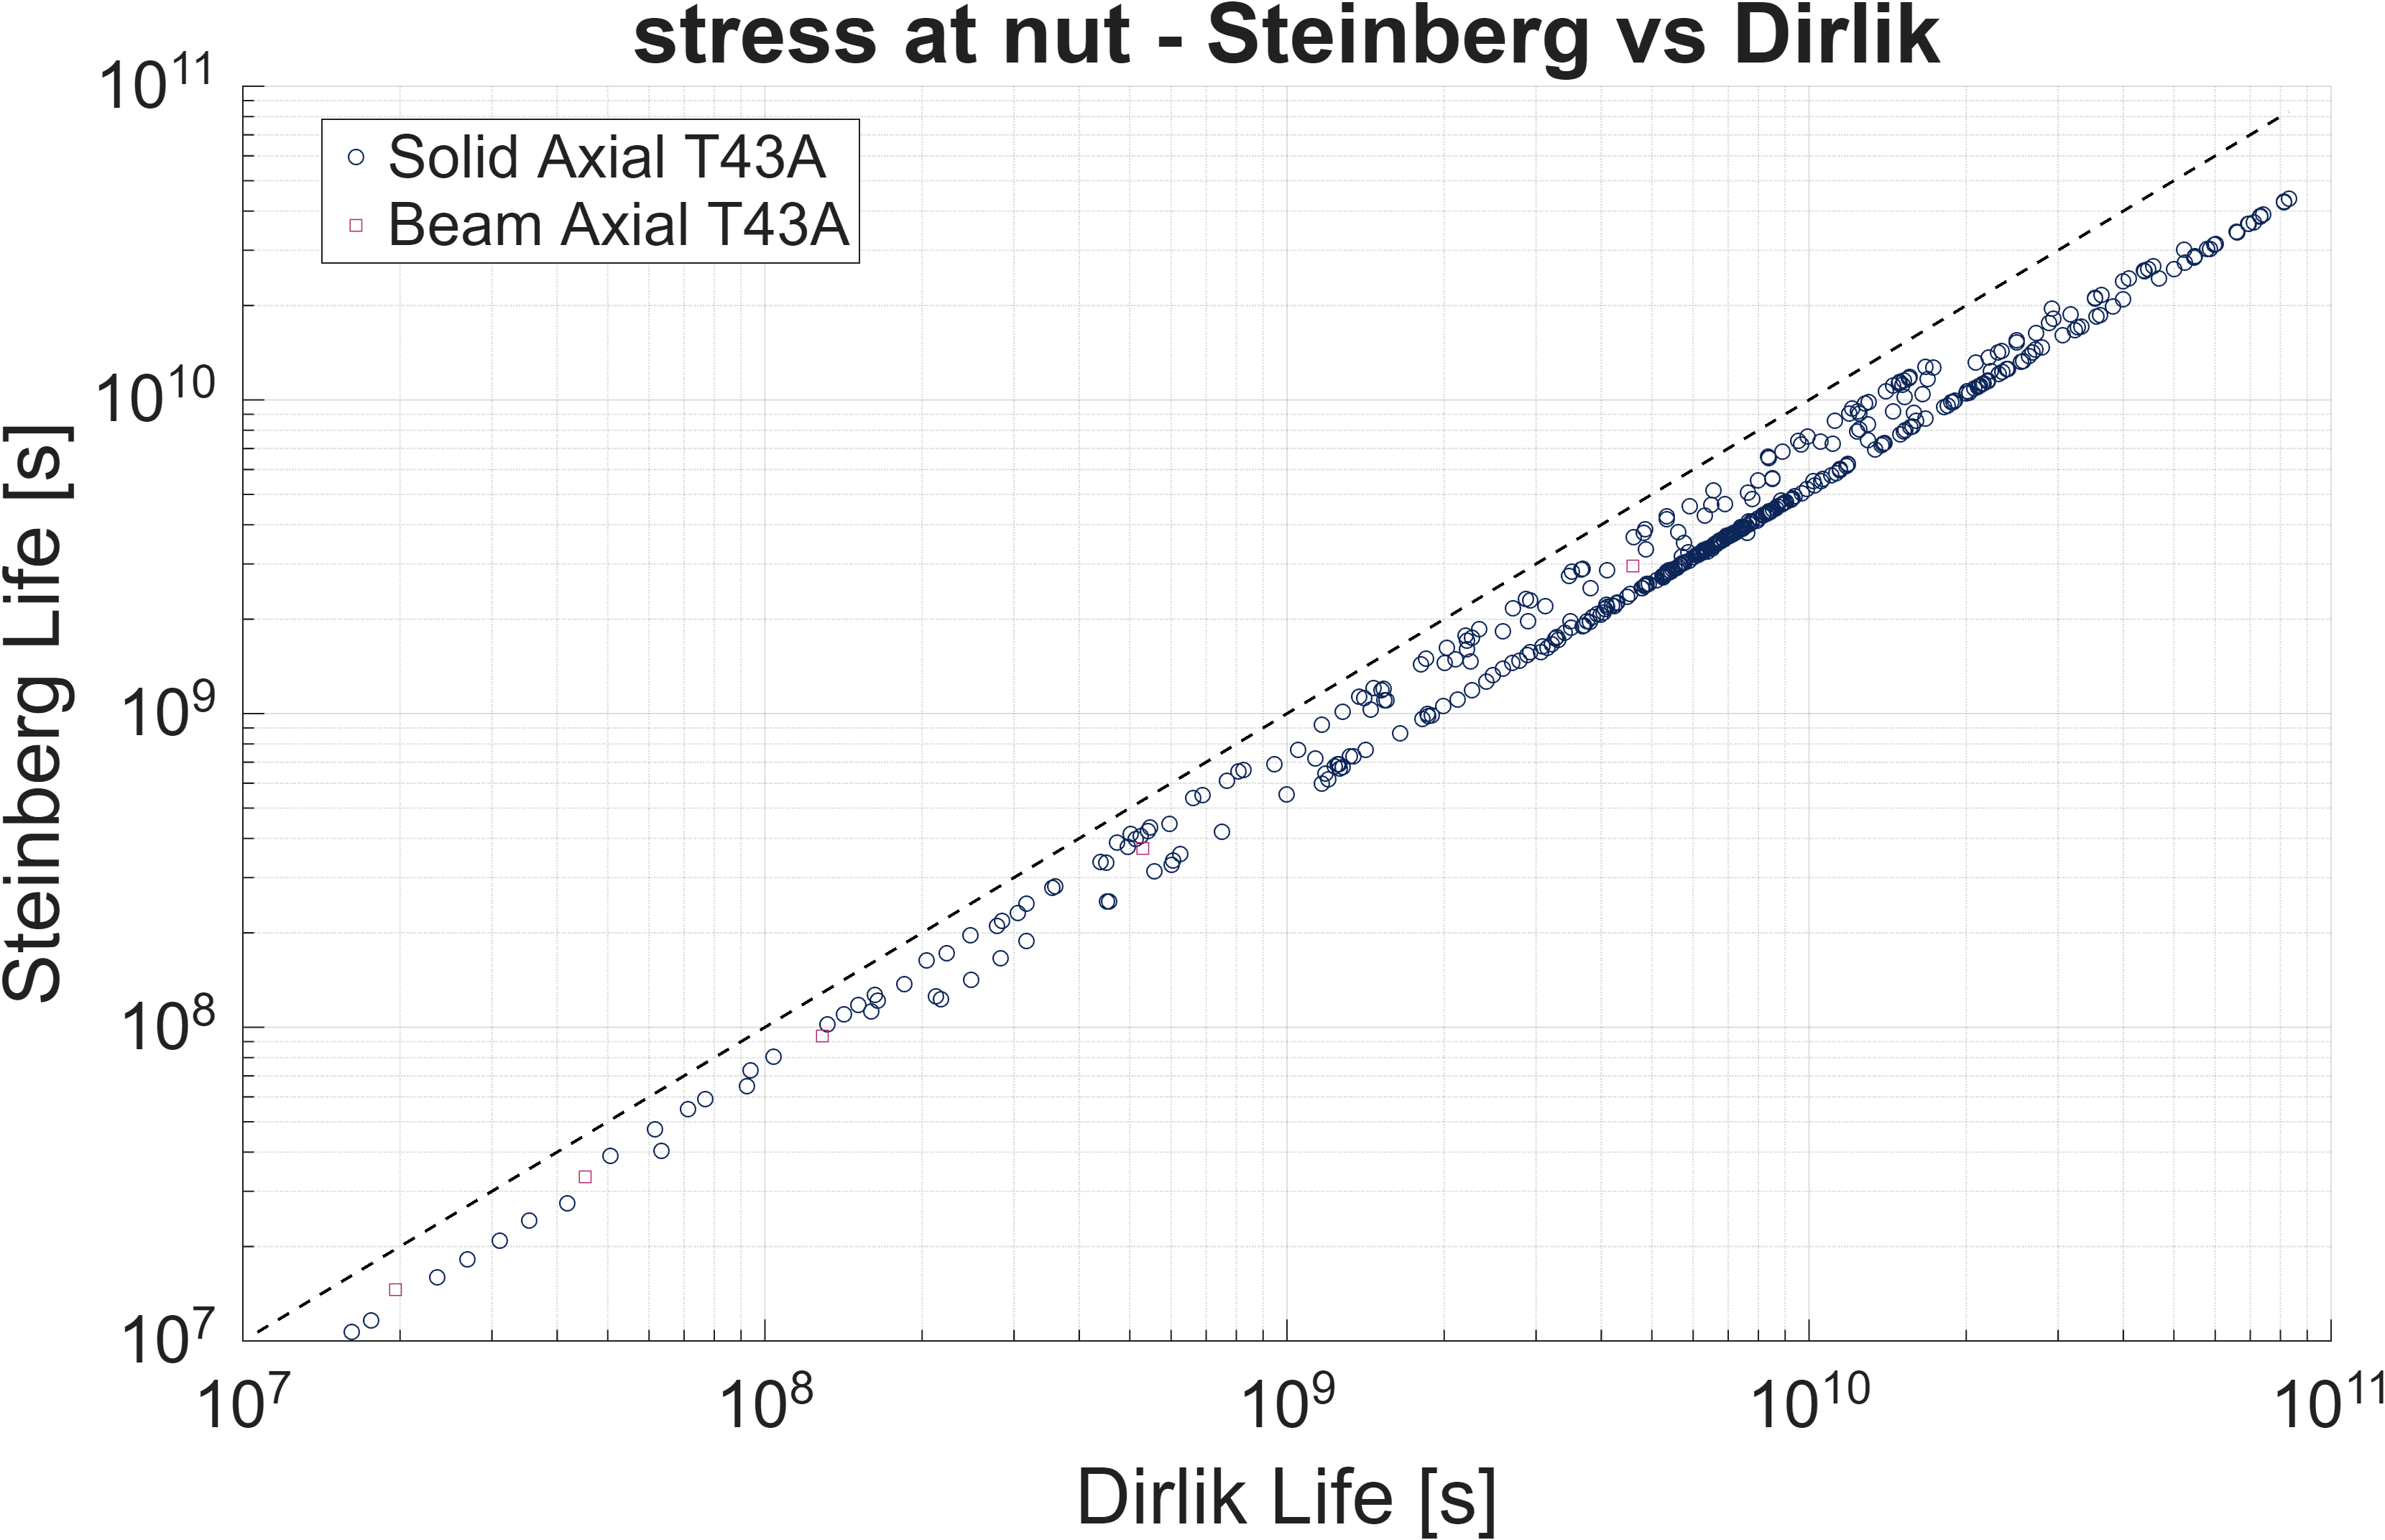
\includegraphics[width=\textwidth]{Axial T43A/Axial T43A_steinberg_vs_dirlik_NODEWISE stress_at_nut.png}
        \caption{Axial Loading (bending).}
        \label{fig:T43A_bending_steinberg_vs_dirlik_NODEWISE_stress_at_nut}
    \end{subfigure}
    
    \caption{Steinberg versus Dirlik fatigue life for the at-nut region (solid model only). Excited by the MIL-STD 810G profile for T43A.}
    \label{fig:SteinbergDirlik_atNut_T43A}
\end{figure}

\begin{figure}[H]
    \centering
    \begin{subfigure}[b]{0.45\textwidth}
        \centering
        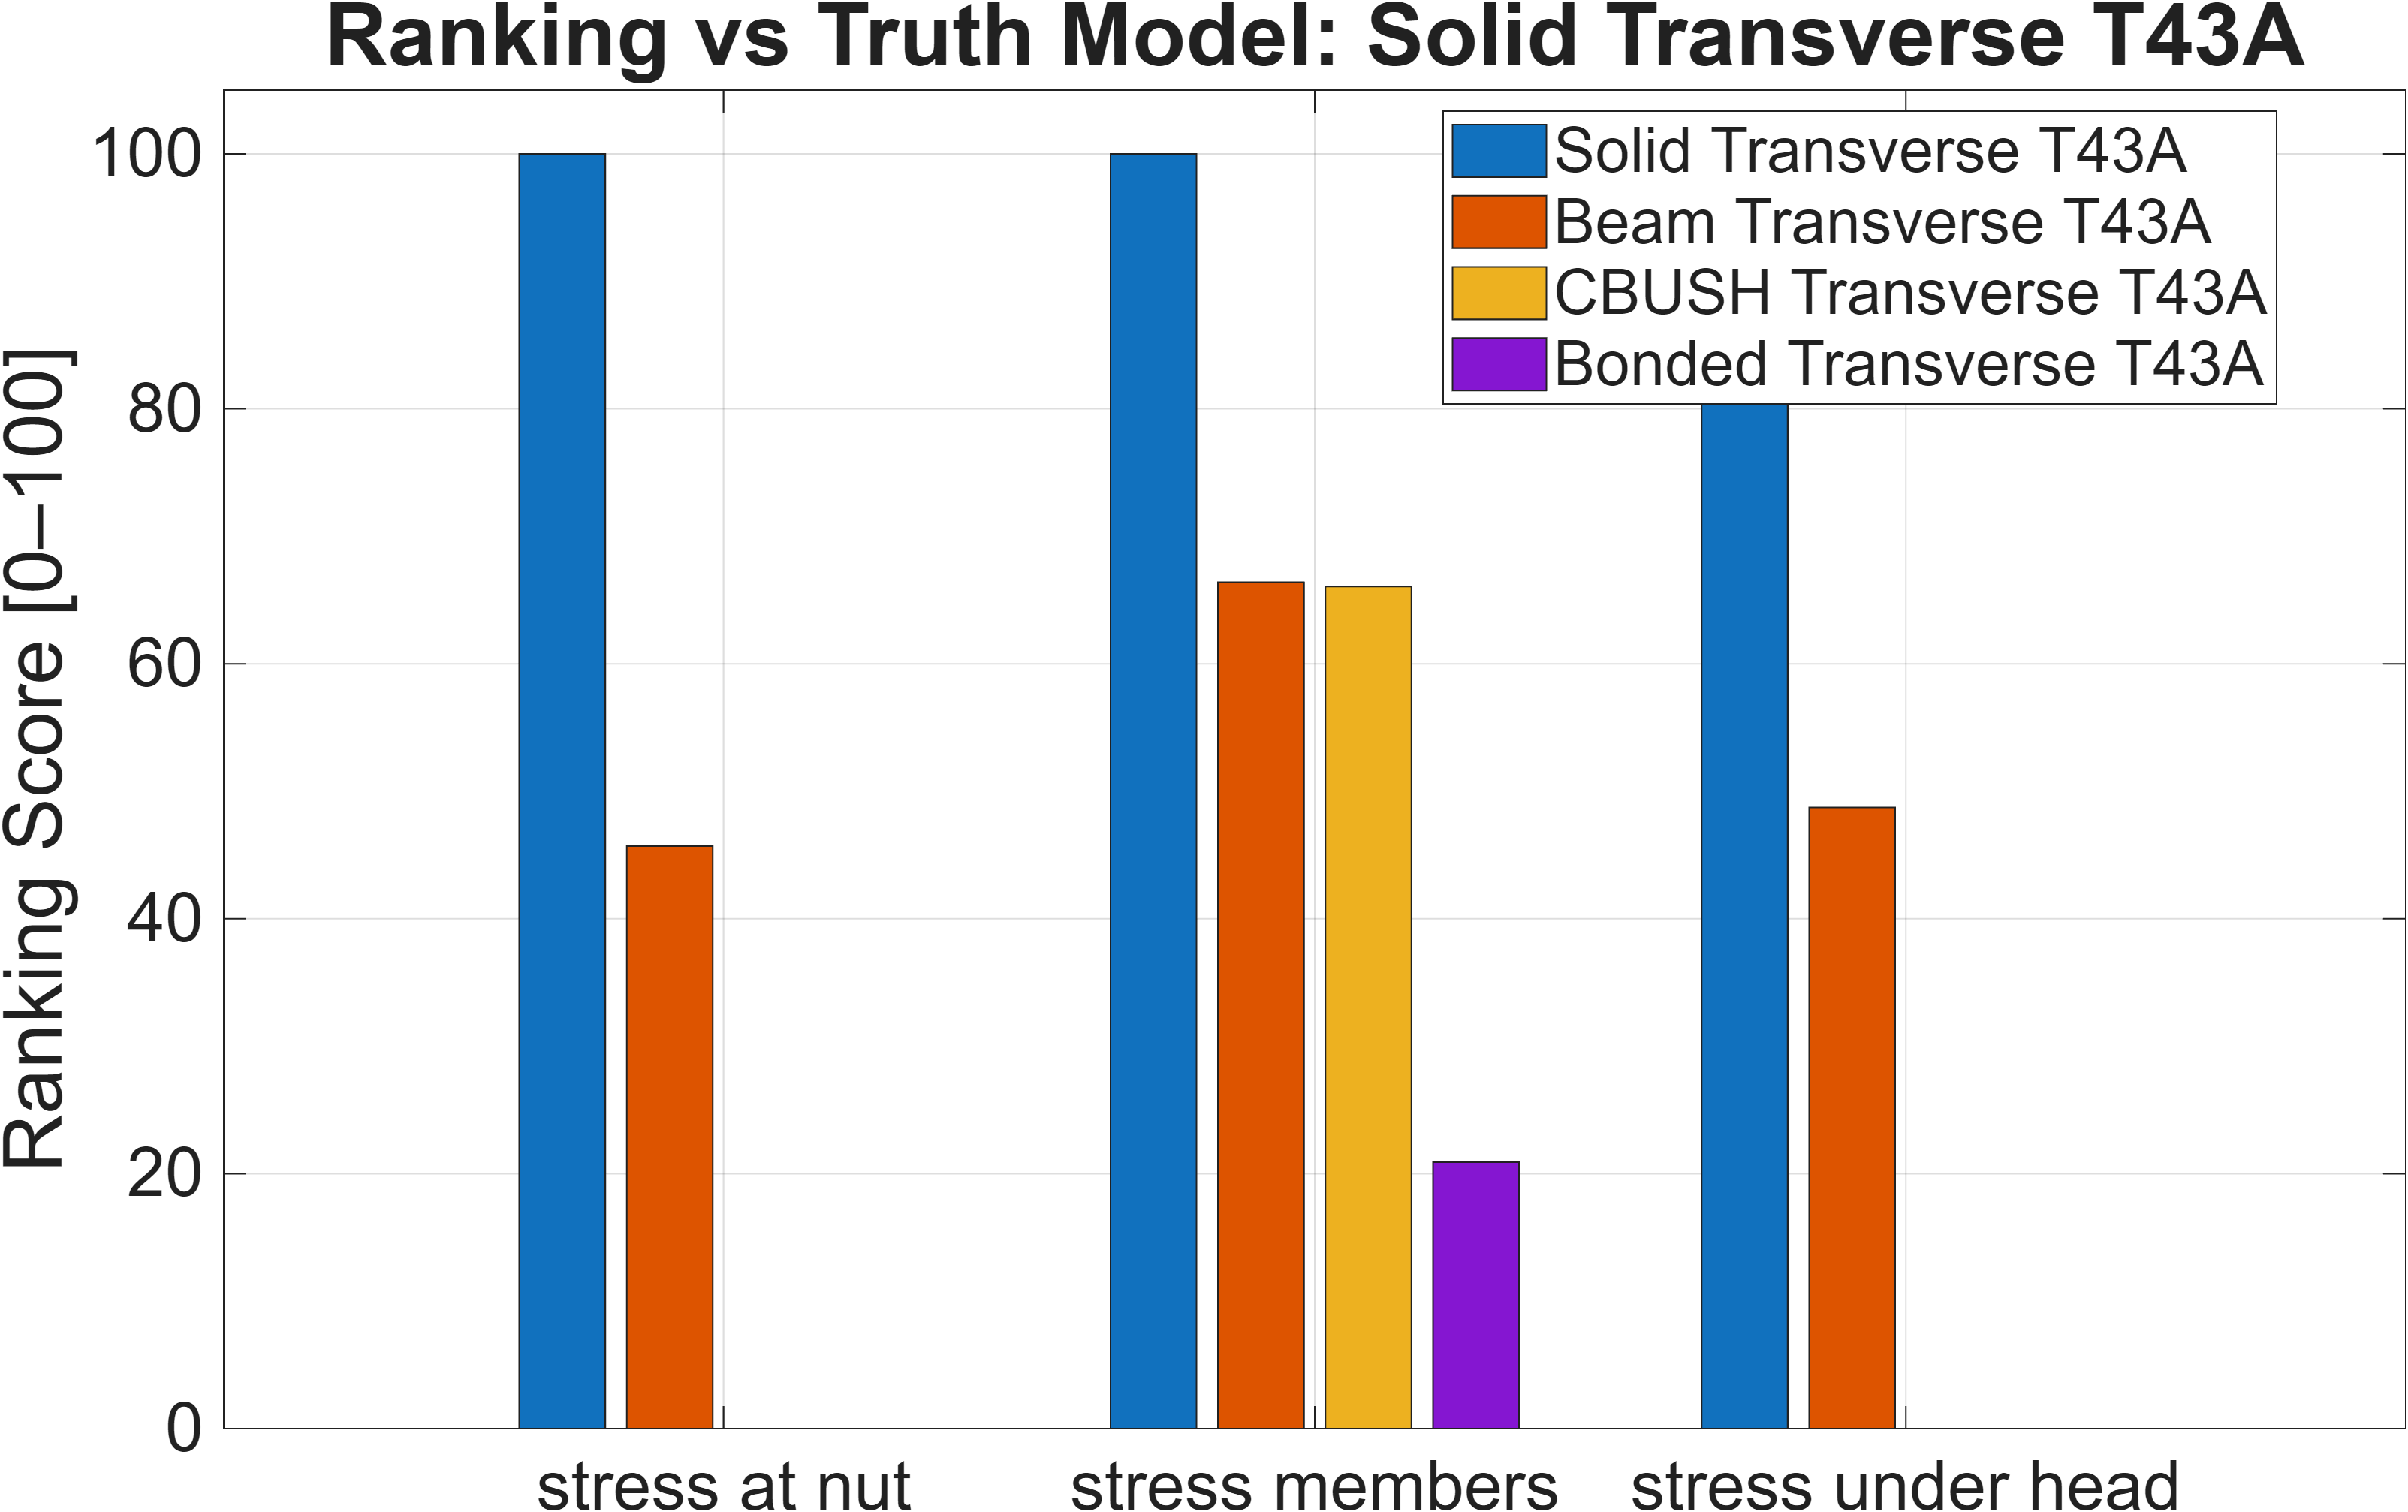
\includegraphics[width=\textwidth]{Transverse T43A/Transverse T43A_ranking_score_by_region_and_model NODEWISE.png}
        \caption{Transverse Loading (shear).}
        \label{fig:T43A_shear_ranking_score_by_region_and_model_NODEWISE}
    \end{subfigure}
    \begin{subfigure}[b]{0.45\textwidth}
        \centering
        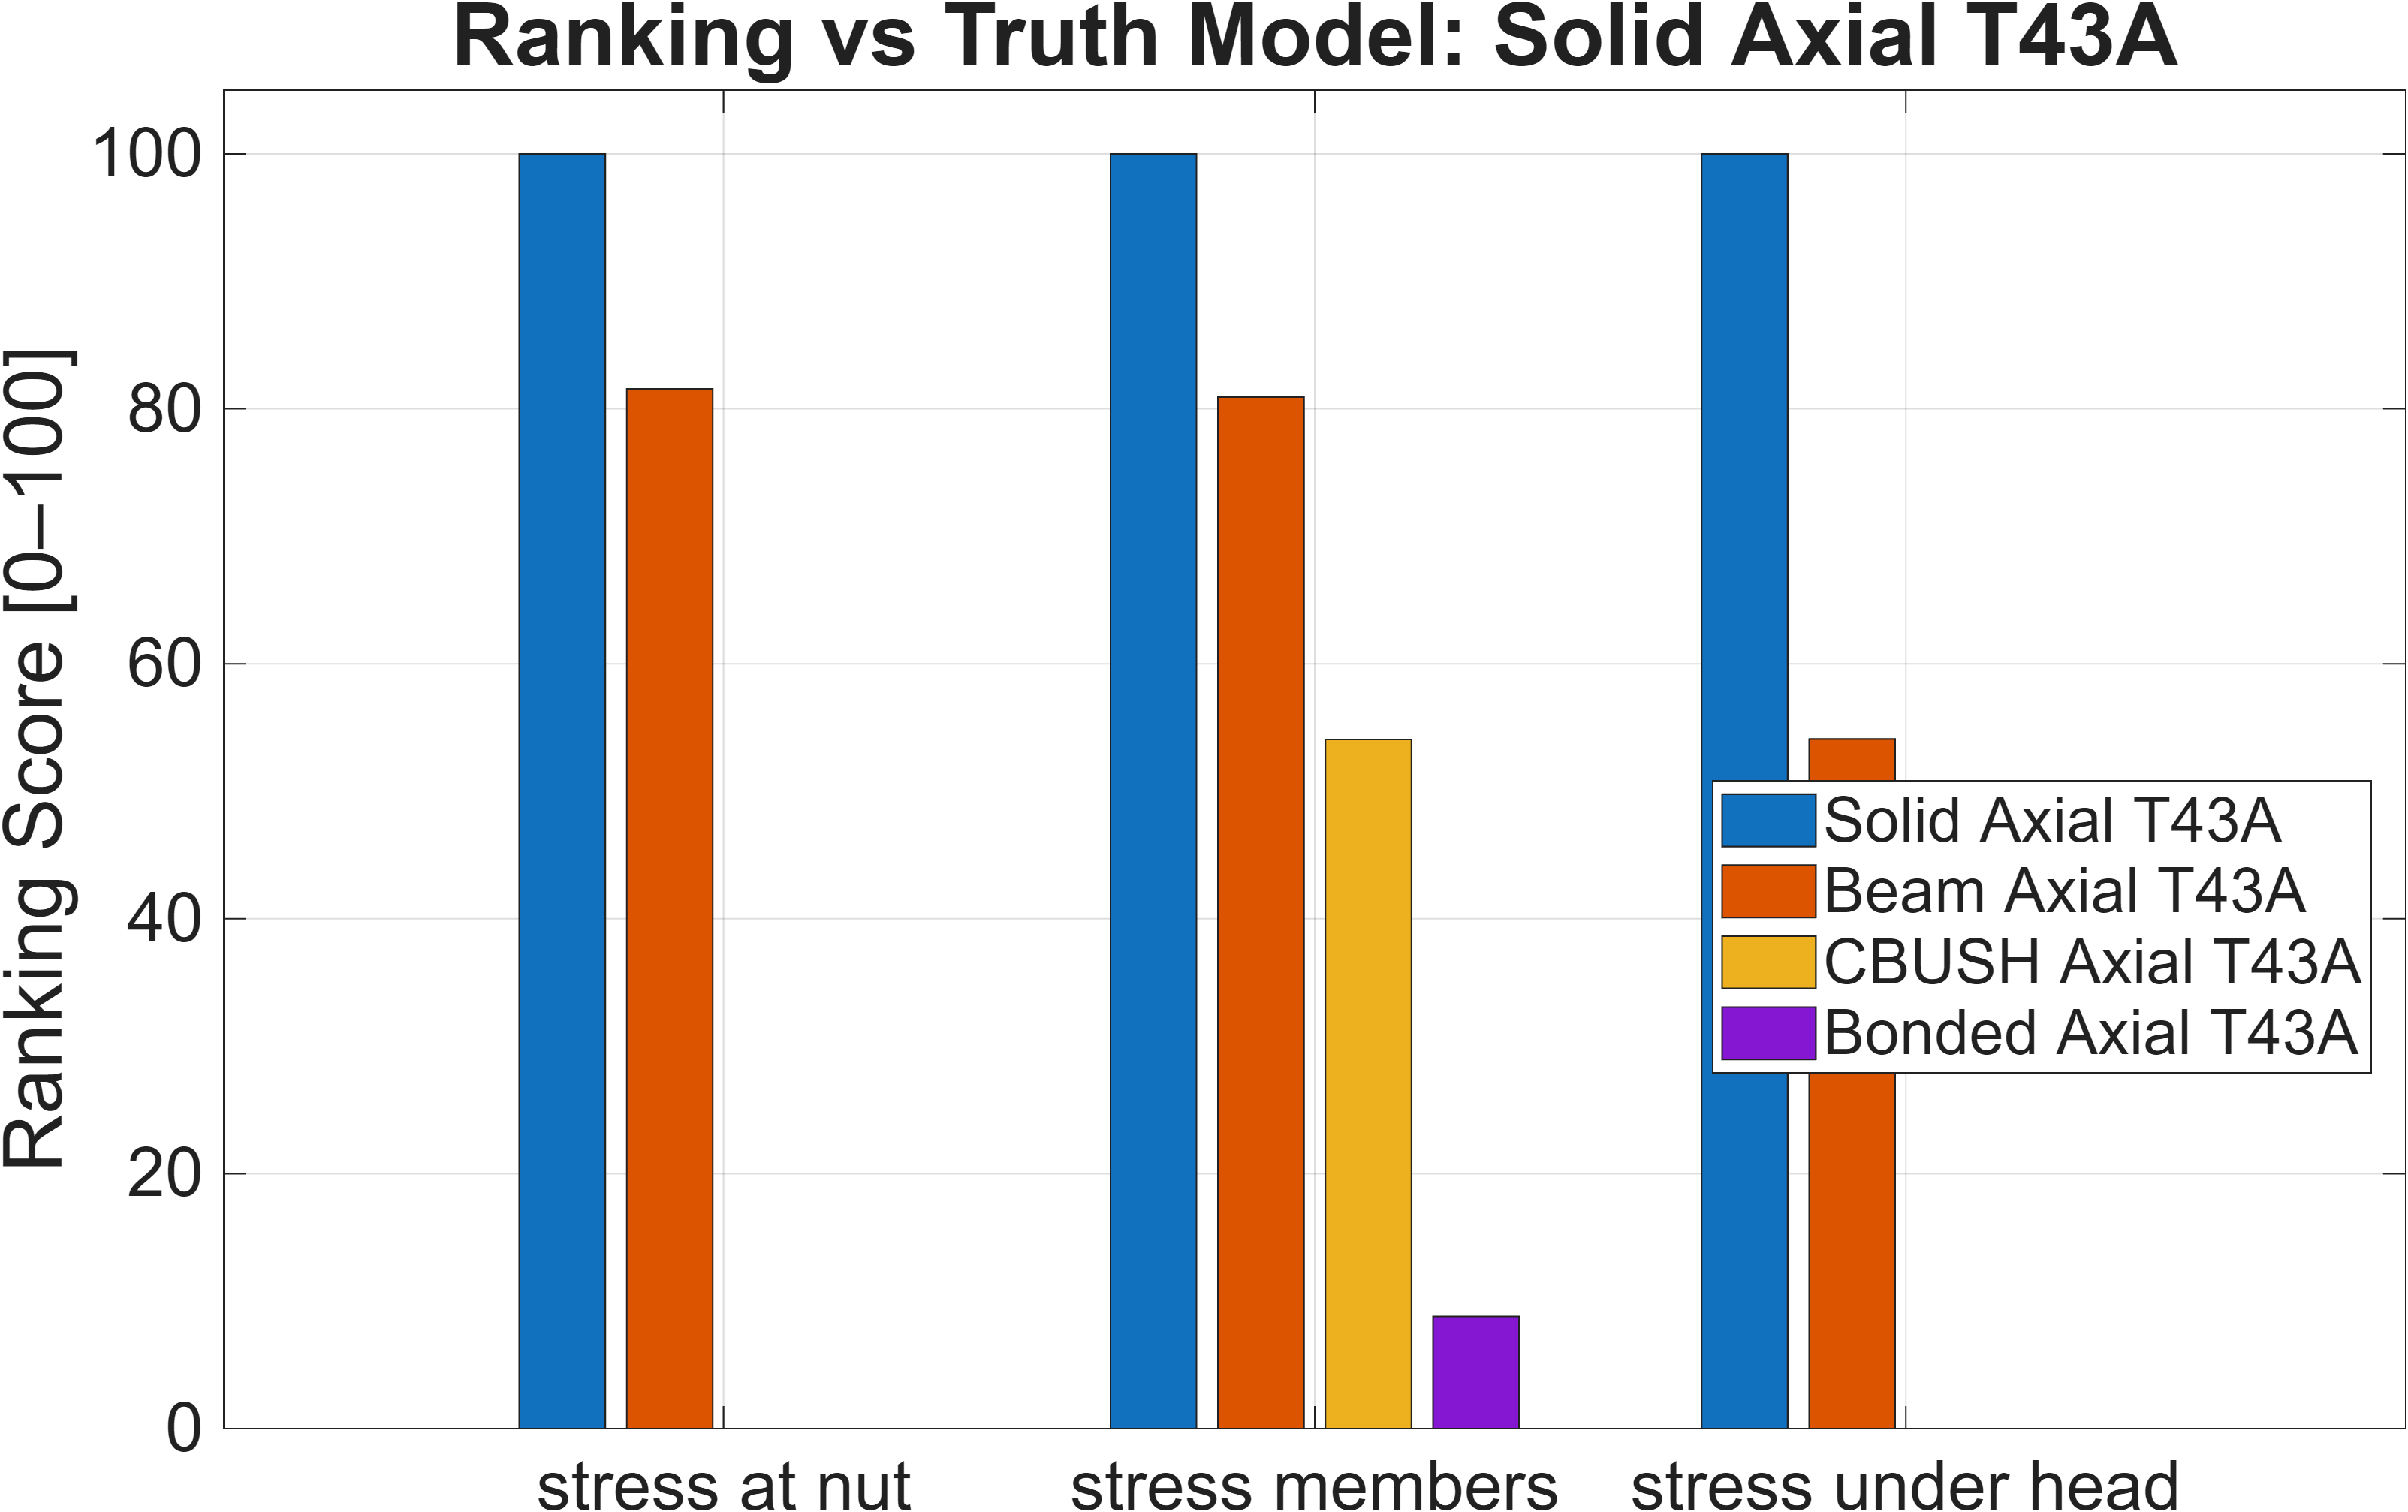
\includegraphics[width=\textwidth]{Axial T43A/Axial T43A_ranking_score_by_region_and_model NODEWISE.png}
        \caption{Axial Loading (bending).}
        \label{fig:T43A_bending_ranking_score_by_region_and_model_NODEWISE}
    \end{subfigure}
    
    \caption{Ranking Index per region and test model, relative to the Solid model. Excited by the MIL-STD 810G profile for T43A.}
    \label{fig:AccuracyScore_per_region_T43A}
\end{figure}

\begin{figure}[H]
    \centering
    \begin{subfigure}[b]{0.45\textwidth}
        \centering
        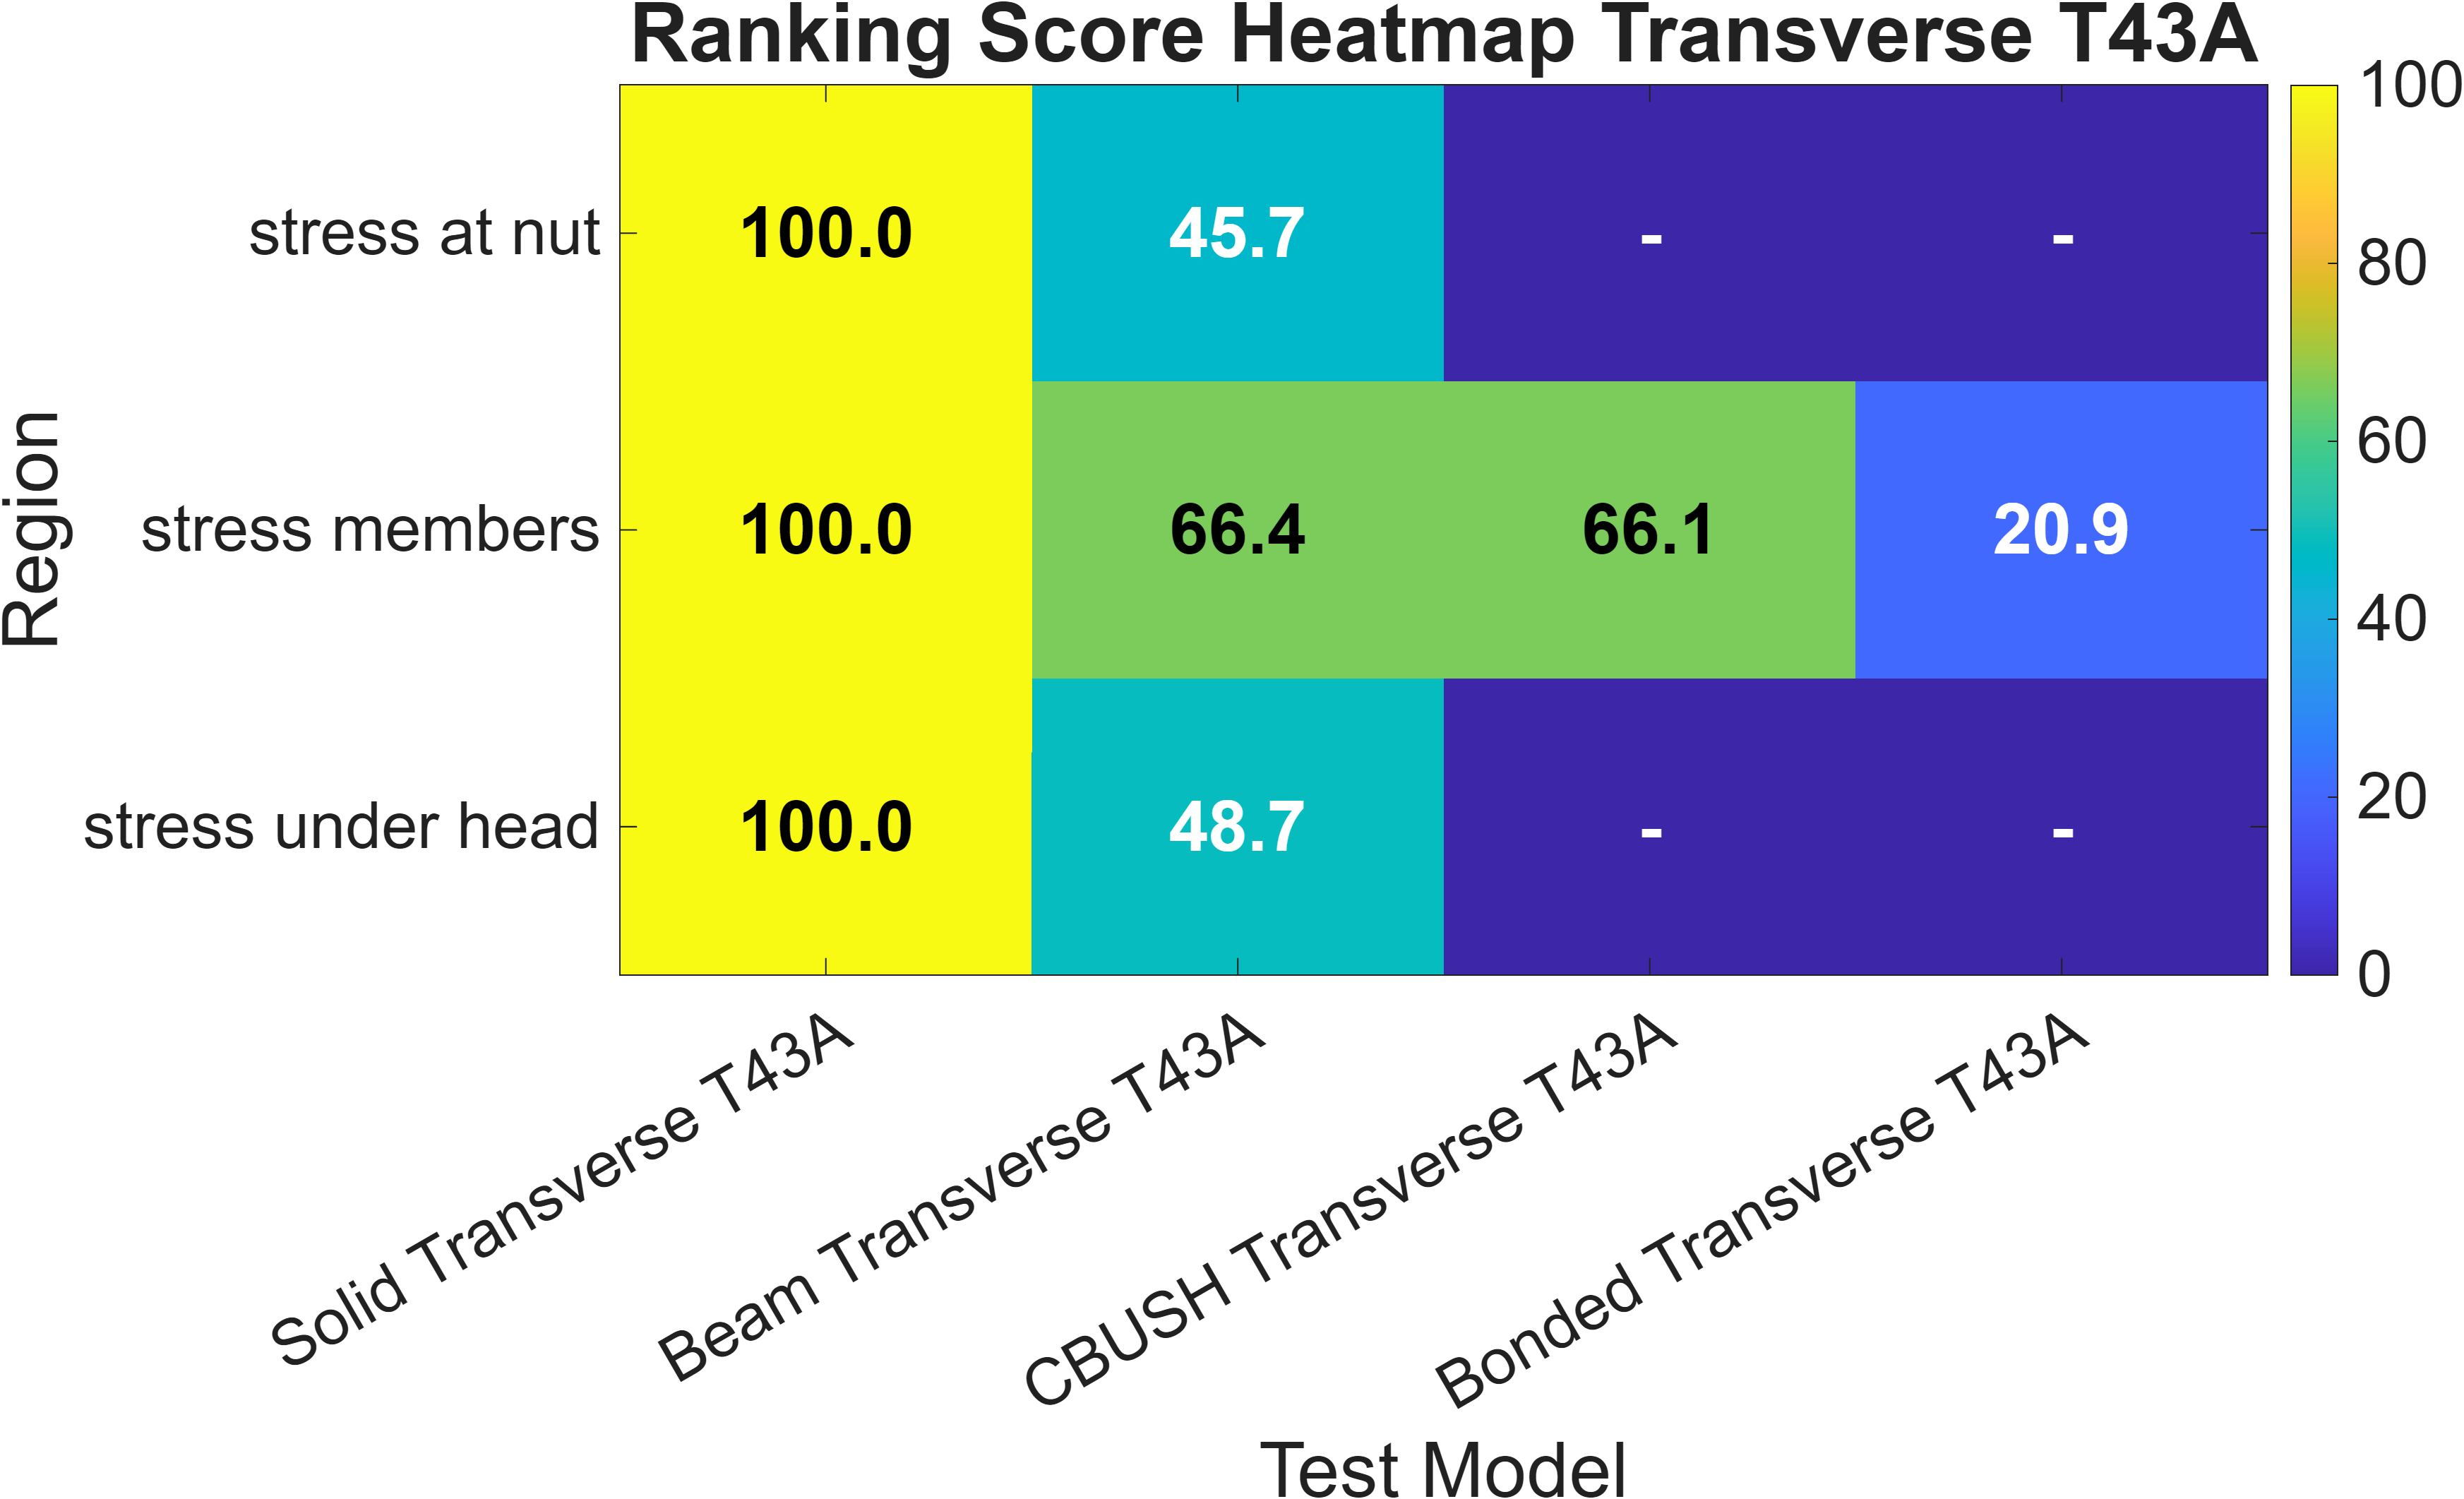
\includegraphics[width=\textwidth]{Transverse T43A/Transverse T43A_ranking_heatmap NODEWISE.png}
        \caption{Transverse Loading (shear).}
        \label{fig:T43A_shear_ranking_heatmap_NODEWISE}
    \end{subfigure}
    \begin{subfigure}[b]{0.45\textwidth}
        \centering
        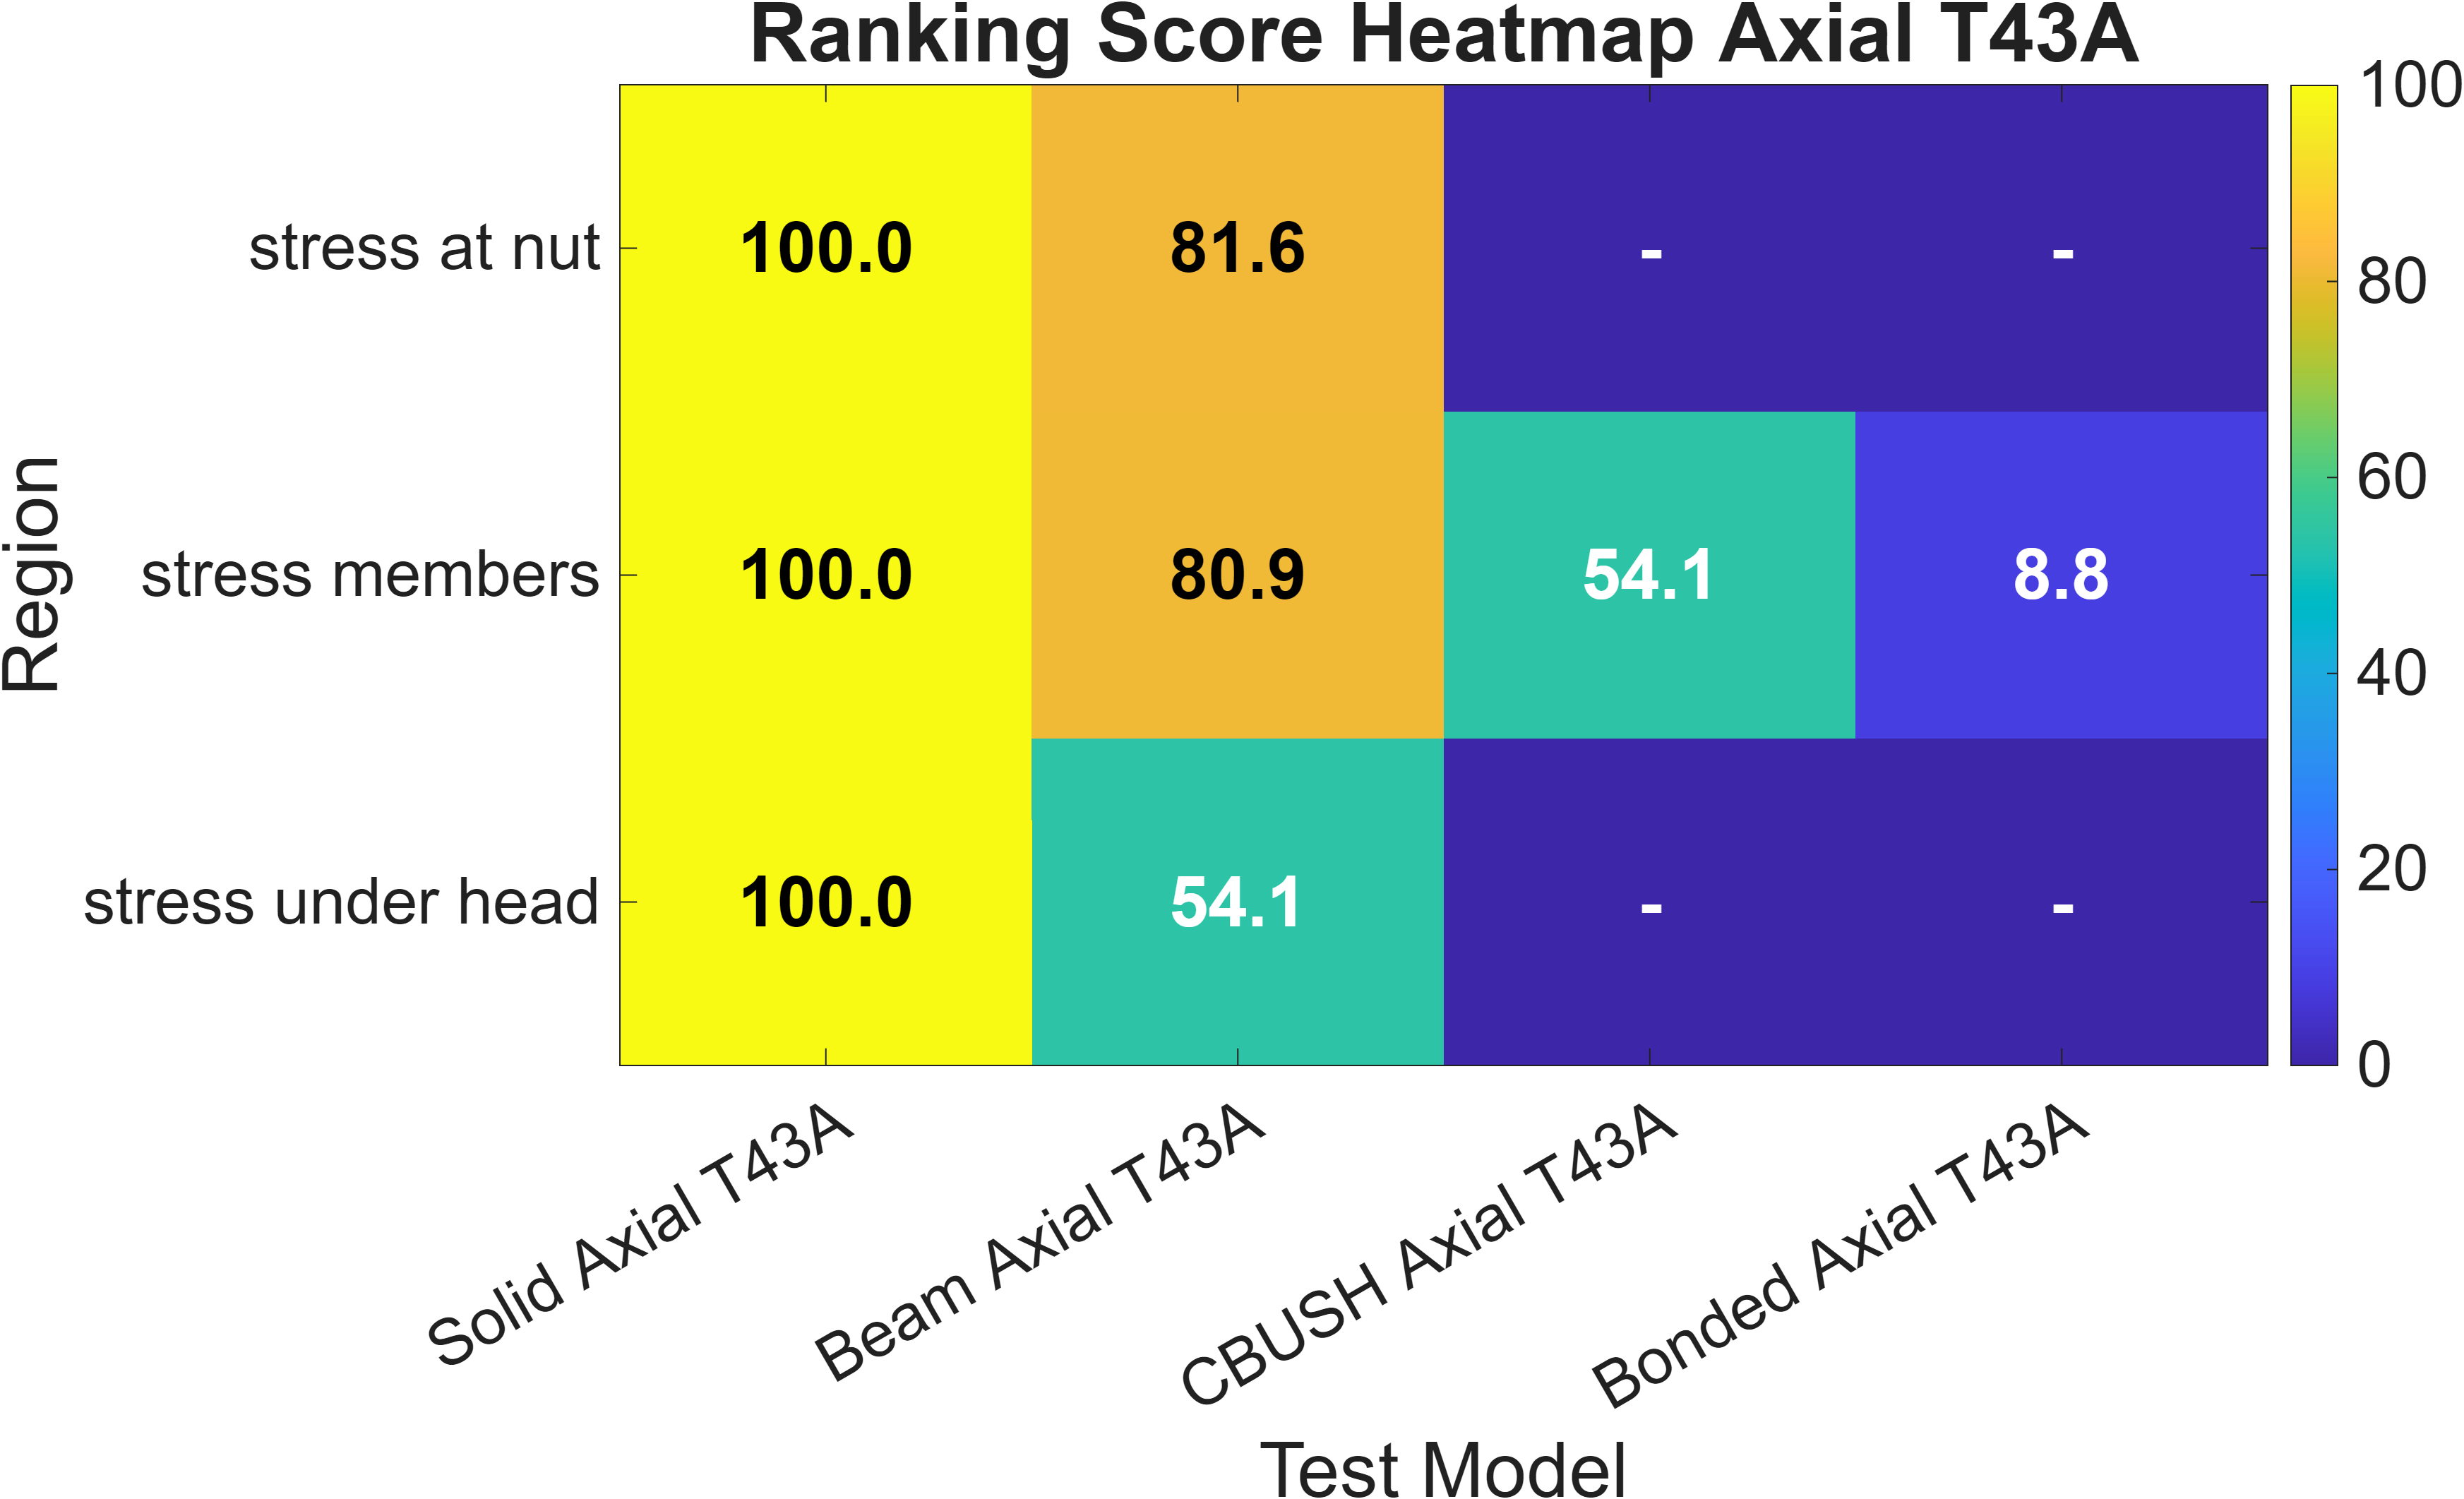
\includegraphics[width=\textwidth]{Axial T43A/Axial T43A_ranking_heatmap NODEWISE.png}
        \caption{Axial Loading (bending).}
        \label{fig:T43A_bending_ranking_heatmap_NODEWISE}
    \end{subfigure}
    
    \caption{Ranking Index heatmap. Excited by the MIL-STD 810G profile for T43A.}
    \label{fig:AccuracyMap_per_region_T43A}
\end{figure}

\begin{figure}[H]
    \centering
    \begin{subfigure}[b]{0.45\textwidth}
        \centering
        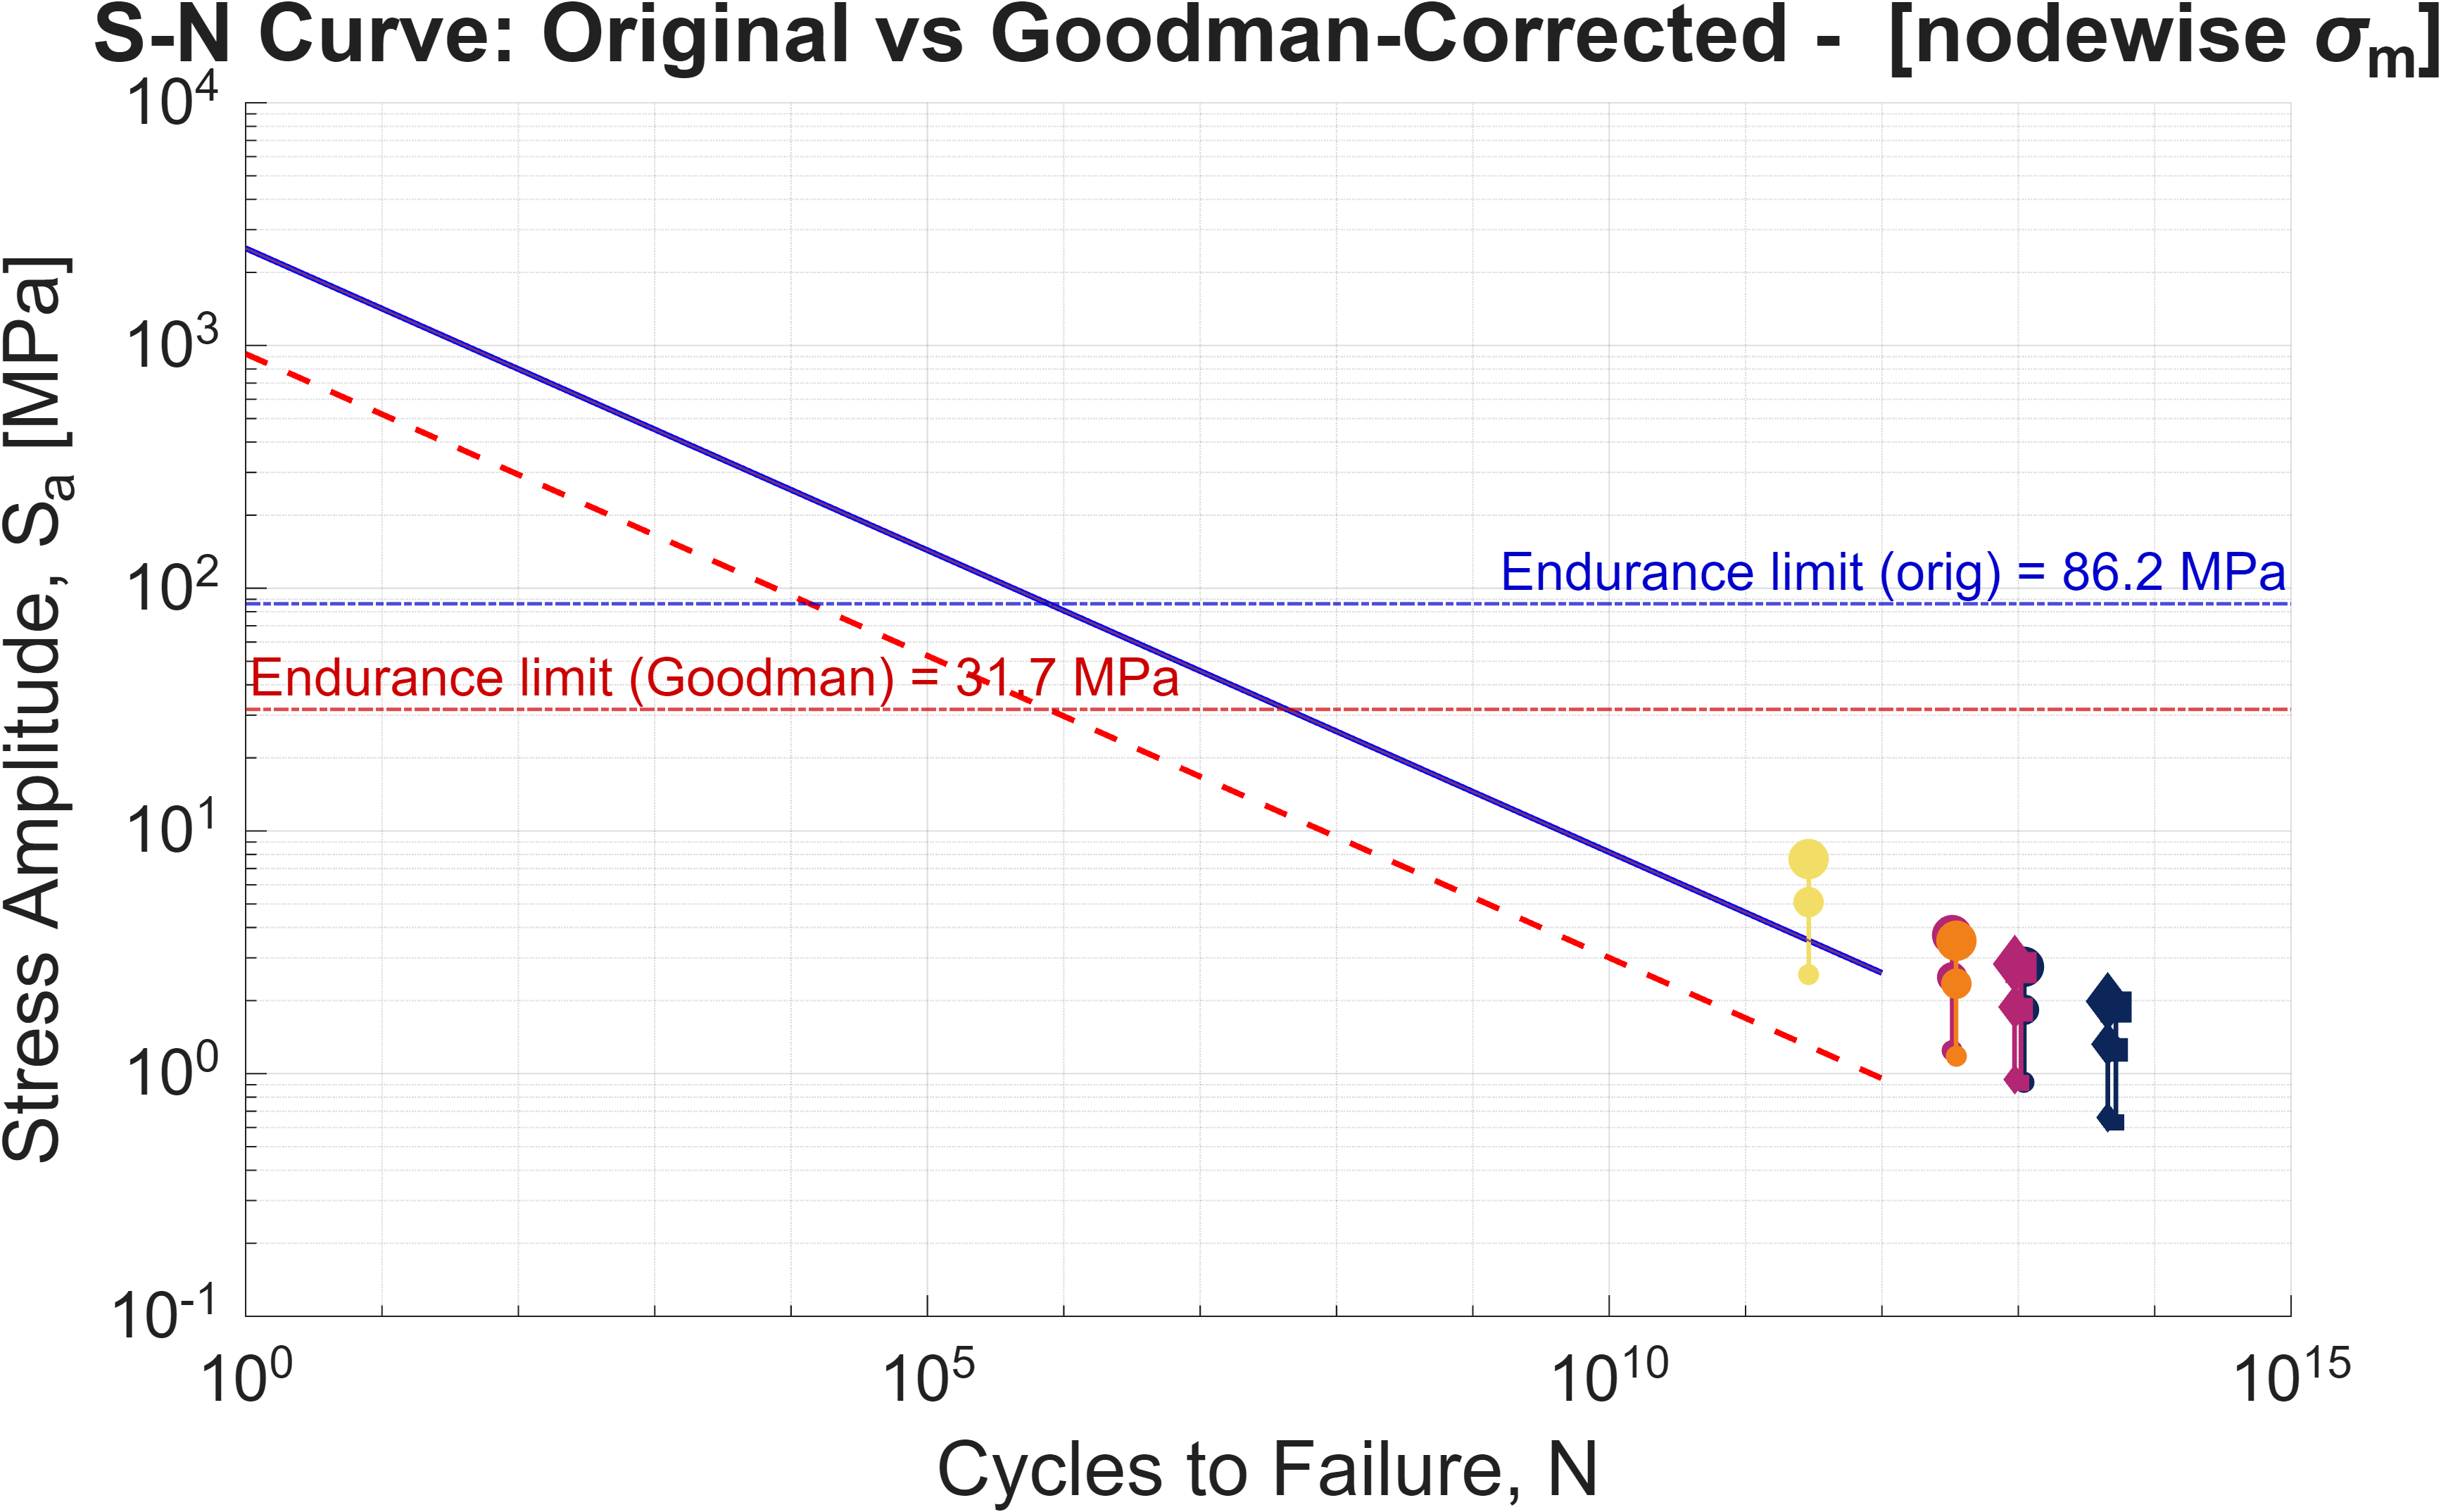
\includegraphics[width=\textwidth]{Transverse T43A/Transverse T43A_sn_curve_goodman_and_rms NODEWISE.png}
        \caption{Transverse Loading (shear).}
        \label{fig:T43A_shear_sn_curve_goodman_and_rms_NODEWISE}
    \end{subfigure}
    \begin{subfigure}[b]{0.45\textwidth}
        \centering
        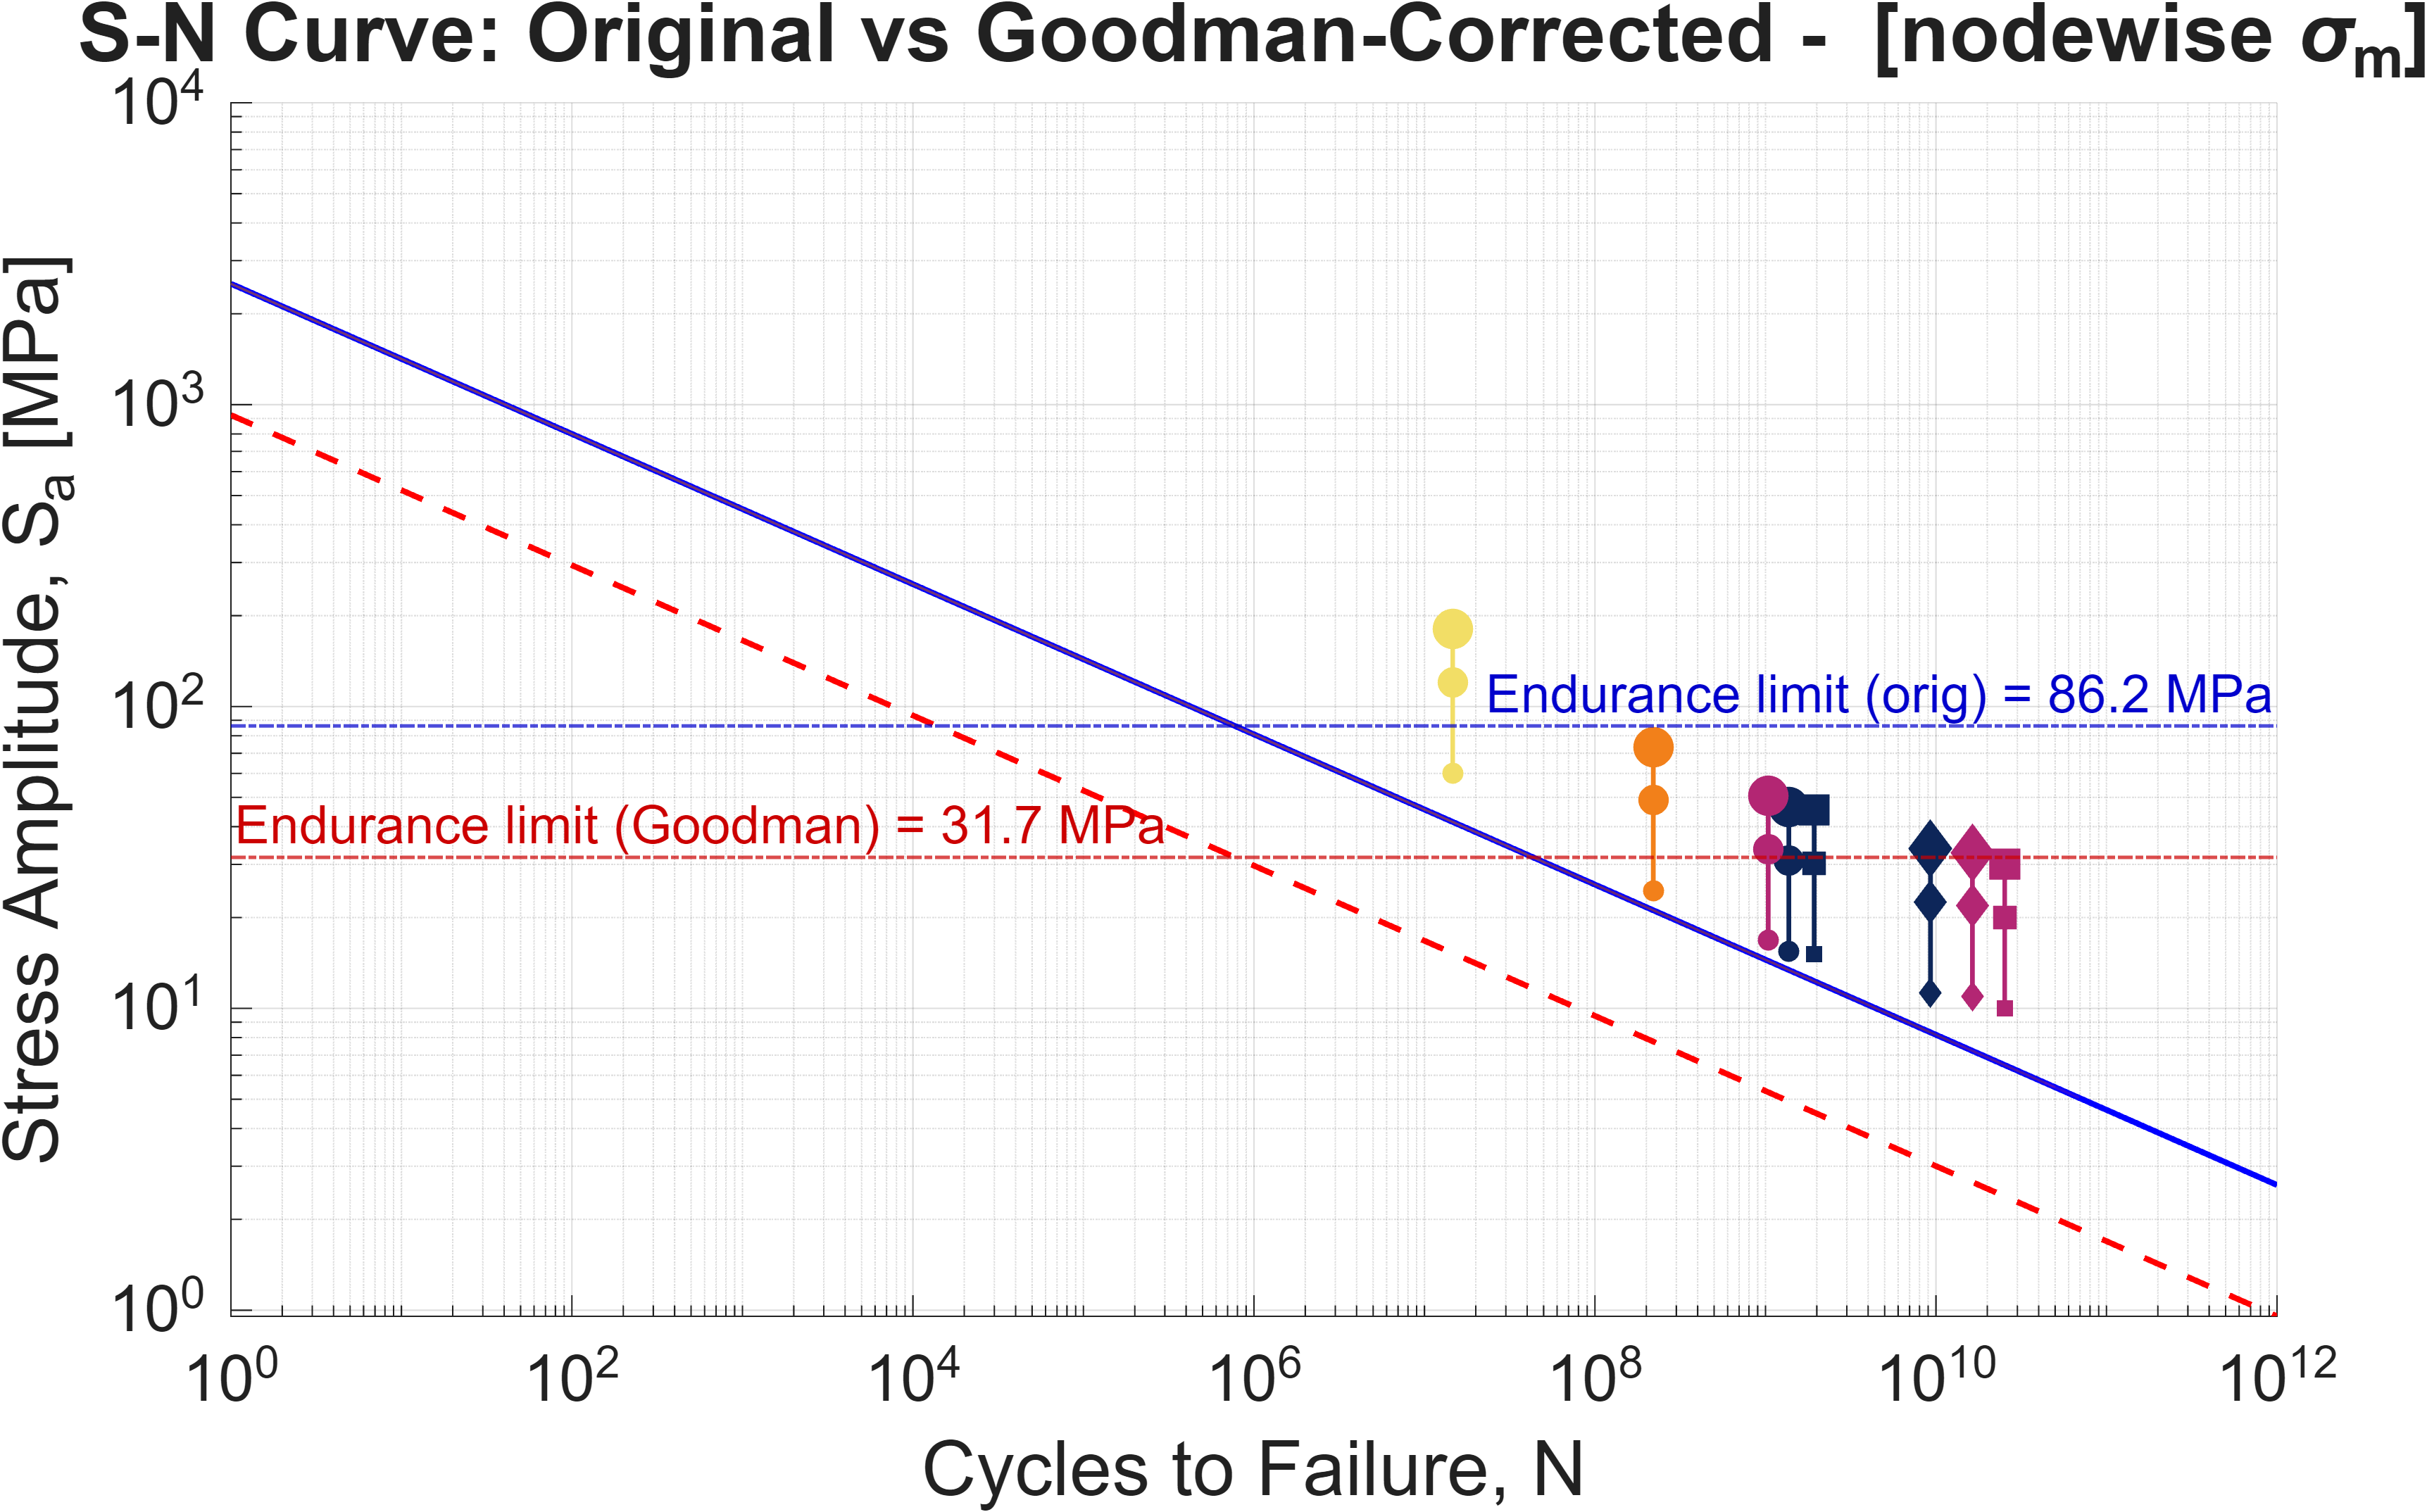
\includegraphics[width=\textwidth]{Axial T43A/Axial T43A_sn_curve_goodman_and_rms NODEWISE.png}
        \caption{Axial Loading (bending).}
        \label{fig:T43A_bending_sn_curve_goodman_and_rms_NODEWISE}
    \end{subfigure}
    
    \caption{SN-diagram with nodewise Goodman correction for the MIL-STD 810G T43A excitation. (a) Transverse loading.  (b) Axial loading.}
    \label{fig:SN_T43A}
\end{figure}


The original SN-curve is shown as a thick solid blue line with a slope parameter of k = 4. A thick dashed red line represents the nominal SN-curve, defined using a mean stress of $\sigma_m$ = 658 MPa and a Goodman factor of $g_f$ = 0.367. The thin lines indicate endurance limits before and after the Goodman correction.
Size of the marker is: small: $1\sigma_{RMS}$, medium: $2\sigma_{RMS}$, large: $3\sigma_{RMS}$.
Size of marker is:
\begin{enumerate}
    \item Small: $1\sigma$
    \item Medium: $1\sigma$
    \item Large: $3\sigma$
\end{enumerate}
Shape of the marker is: 
\begin{enumerate}
    \item Circular: Clamped-members
    \item Square: Under-head fillet
    \item Diamond: First-engaged-thread region.
\end{enumerate}
Color of the marker is:
\begin{enumerate}
    \item Yellow: Bonded
    \item Orange: CBUSH
    \item Pink: Beam
    \item Dark blue: Solid
\end{enumerate}


\chapter{SN-curve} \label{app:SN-curve}
Figure \ref{fig:SN_NASA} and \ref{fig:SN_T43A} show the SN fatigue assessment for all four loading cases. In each subplot, the power-law SN-curve is shown alongside the Goodman-corrected curve. To assess whether the predicted fatigue lives are finite or infinite, the critical nodes are compared to the SN-curve above. Two variants of the modified Goodman correction are compared: a nominal approach, in which a uniform mean stress $\sigma_m = 0.7 R_{p0.2} = 658$ MPa is applied to every node, and a nodewise approach, in which the per-node static von Mises stress from the preload analysis is used as $\sigma_m$. In both cases, the Goodman factor is $g_f = 1- \tfrac{\sigma_m}{\sigma_u}$, and for each node $n$ the SN is scaled as $C_{eff} = (C\cdot g_f^k)_n$.

The modified Goodman correction accounts for the nominal bolt preload stress, taken as $\sigma_m = 0.7 R_{p0.2} = 658$ MPa, which gives a correction factor $g_f = 1- \tfrac{\sigma_m}{\sigma_u} = 0.367$. As a result, the allowable stress amplitude is reduced by a factor of approximately $1/0.367 = 2.7$. At the conventional reference life of $N_{ref} = 10^6$ cycles, this reduces the nominal endurance limit from $S_{nom} = (\tfrac{C}{N_{ref}})^{1/k} \approx 82$ MPa to $S_{corr} = g_f \cdot S_{nom} \approx 30$ MPa.

In Figure \ref{fig:SN_NASA}, the SN-line is the continuous power-law $S=CN^{1/k}$, with $C=4.6\times 10^{13}$ and $k=4$. The transverse axis is expected cycles to failure, computed for each node as the Dirlik fatigue life (in seconds) multiplied by the node's peak rate, $\nu_p = \sqrt{m_4/m_2}$. This is the same as the Dirlik damage method used internally. For a narrowband vibration, this rate equals the dominant frequency, and a position ($N; \sigma_{rms}$) can be read as the equivalent constant-amplitude test that would produce the same expected life.

\begin{figure}[H]
    \centering
    \begin{subfigure}[b]{0.45\textwidth}
        \centering
        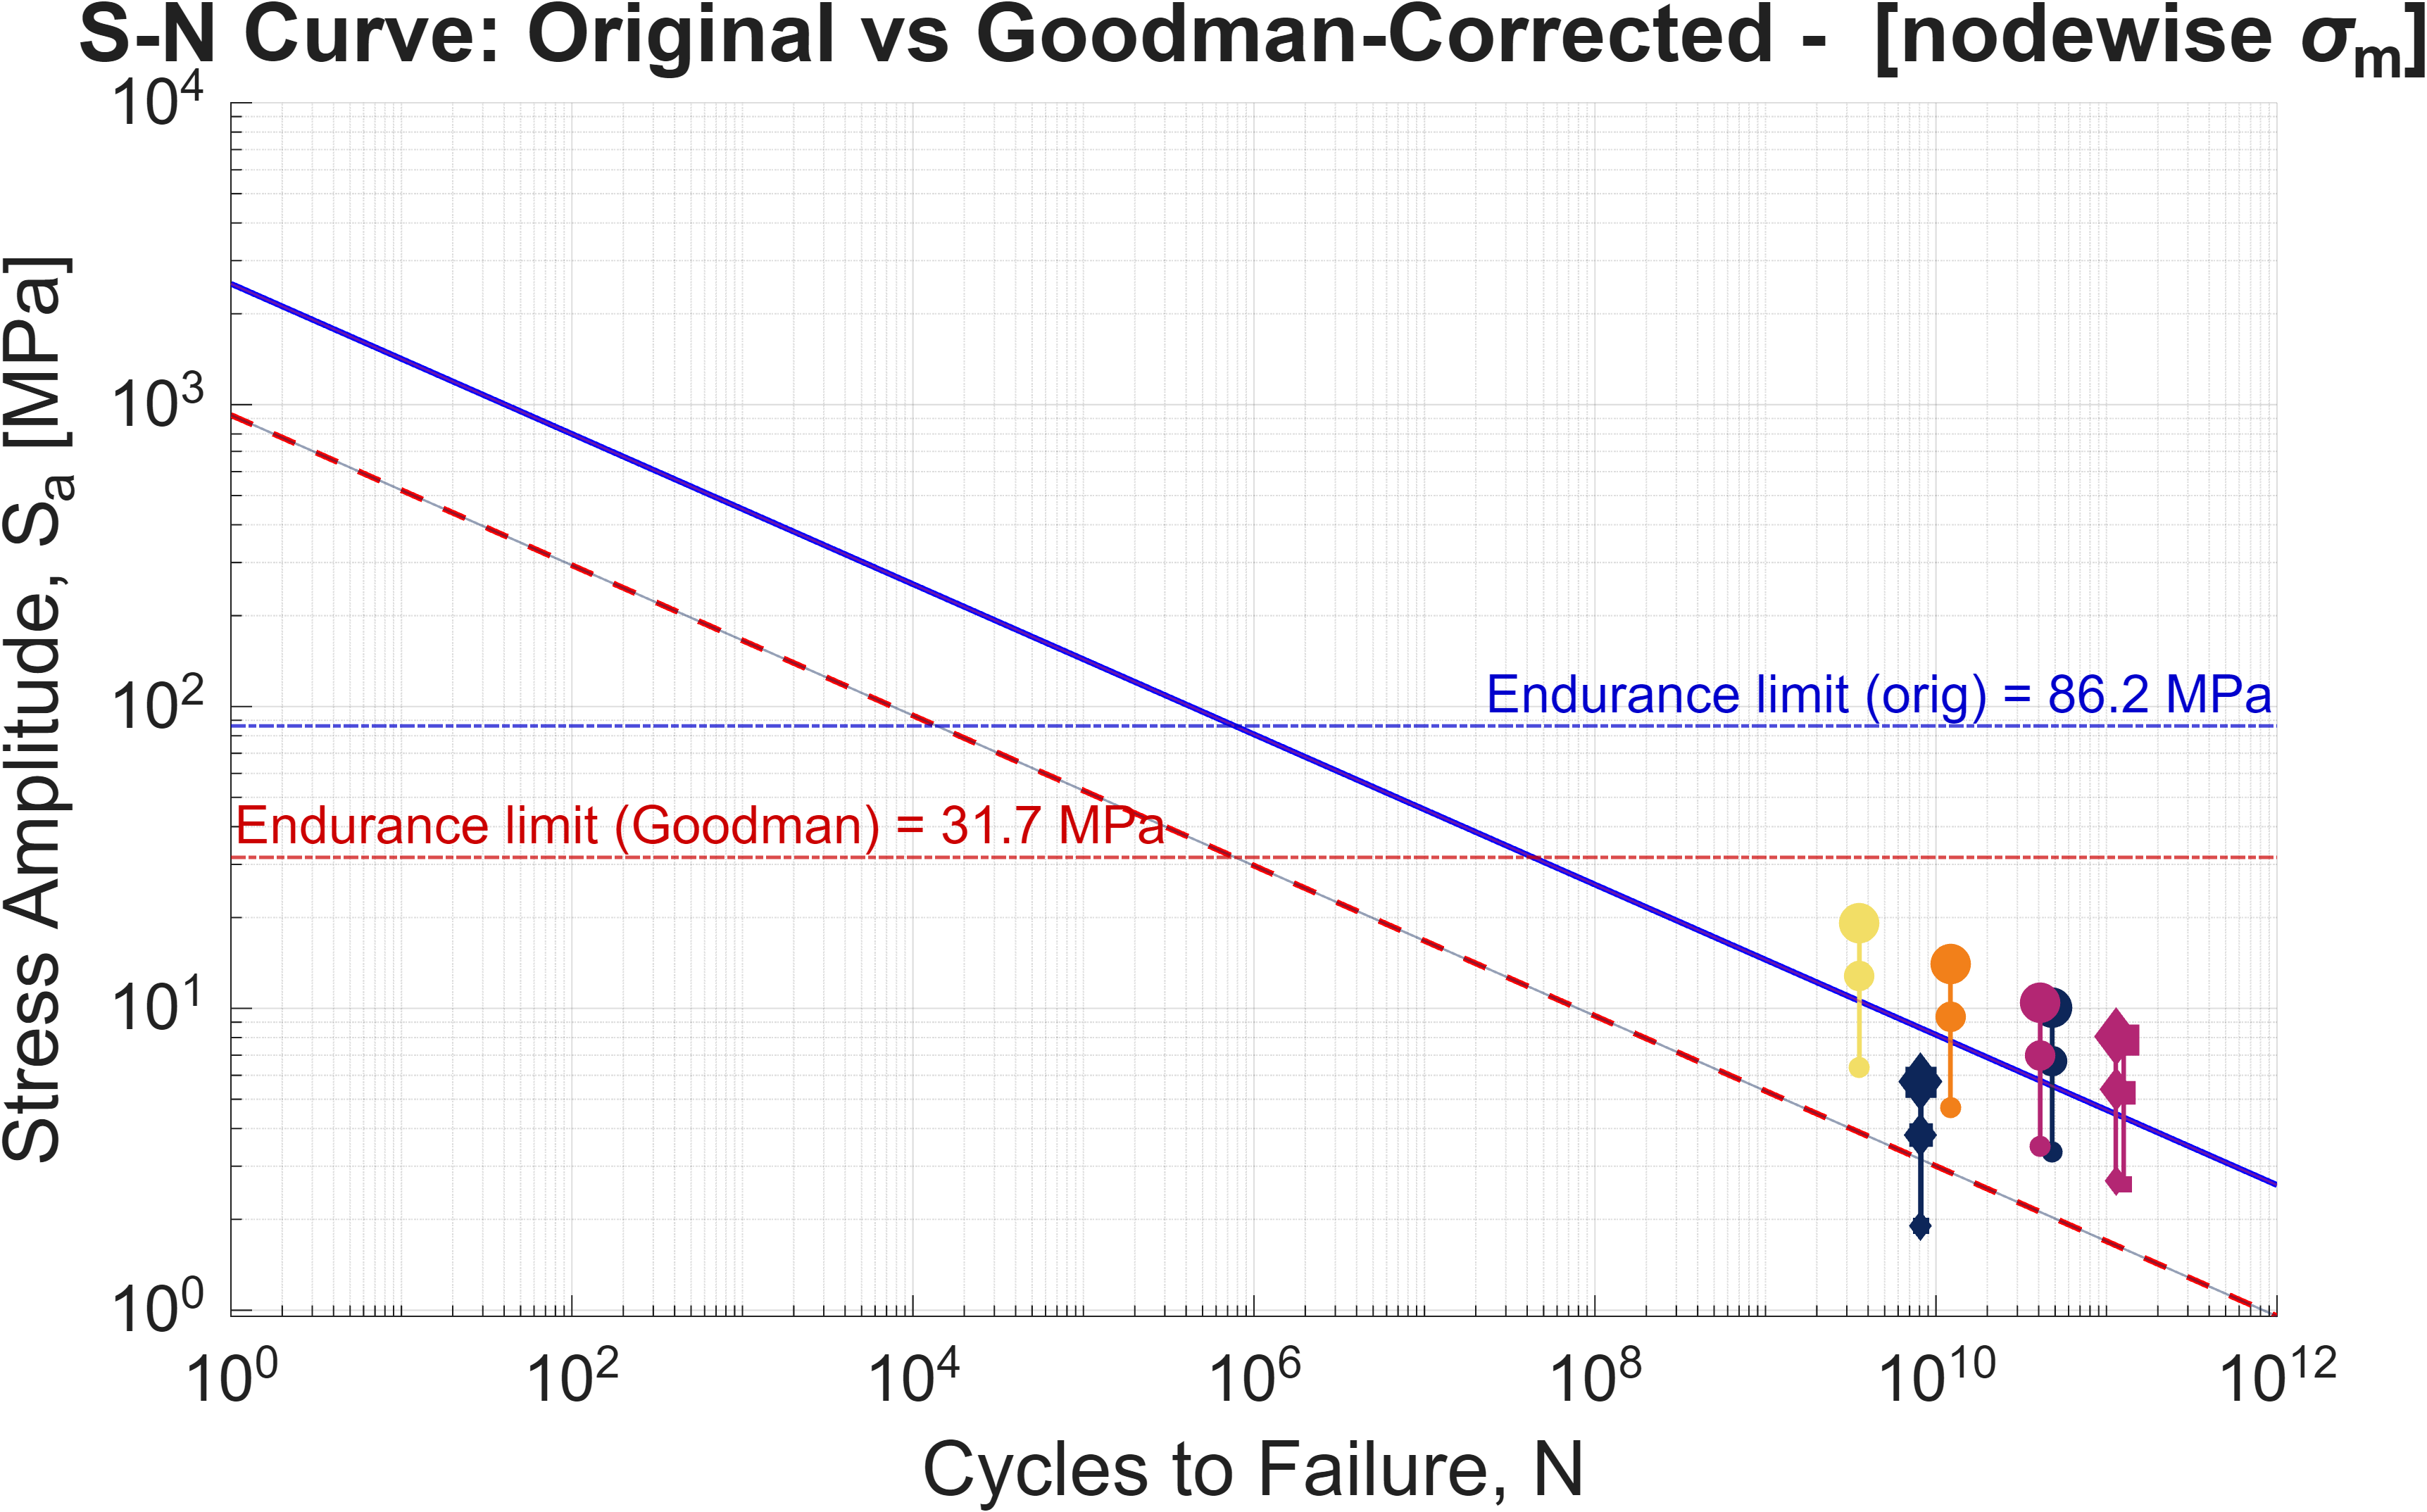
\includegraphics[width=\textwidth]{Transverse Nasa/Transverse Nasa_sn_curve_goodman_and_rms NODEWISE.png}
        \caption{Transverse Loading (shear).}
        \label{fig:NASA_shear_sn_curve_goodman_and_rms_NODEWISE}
    \end{subfigure}
    \begin{subfigure}[b]{0.45\textwidth}
        \centering
        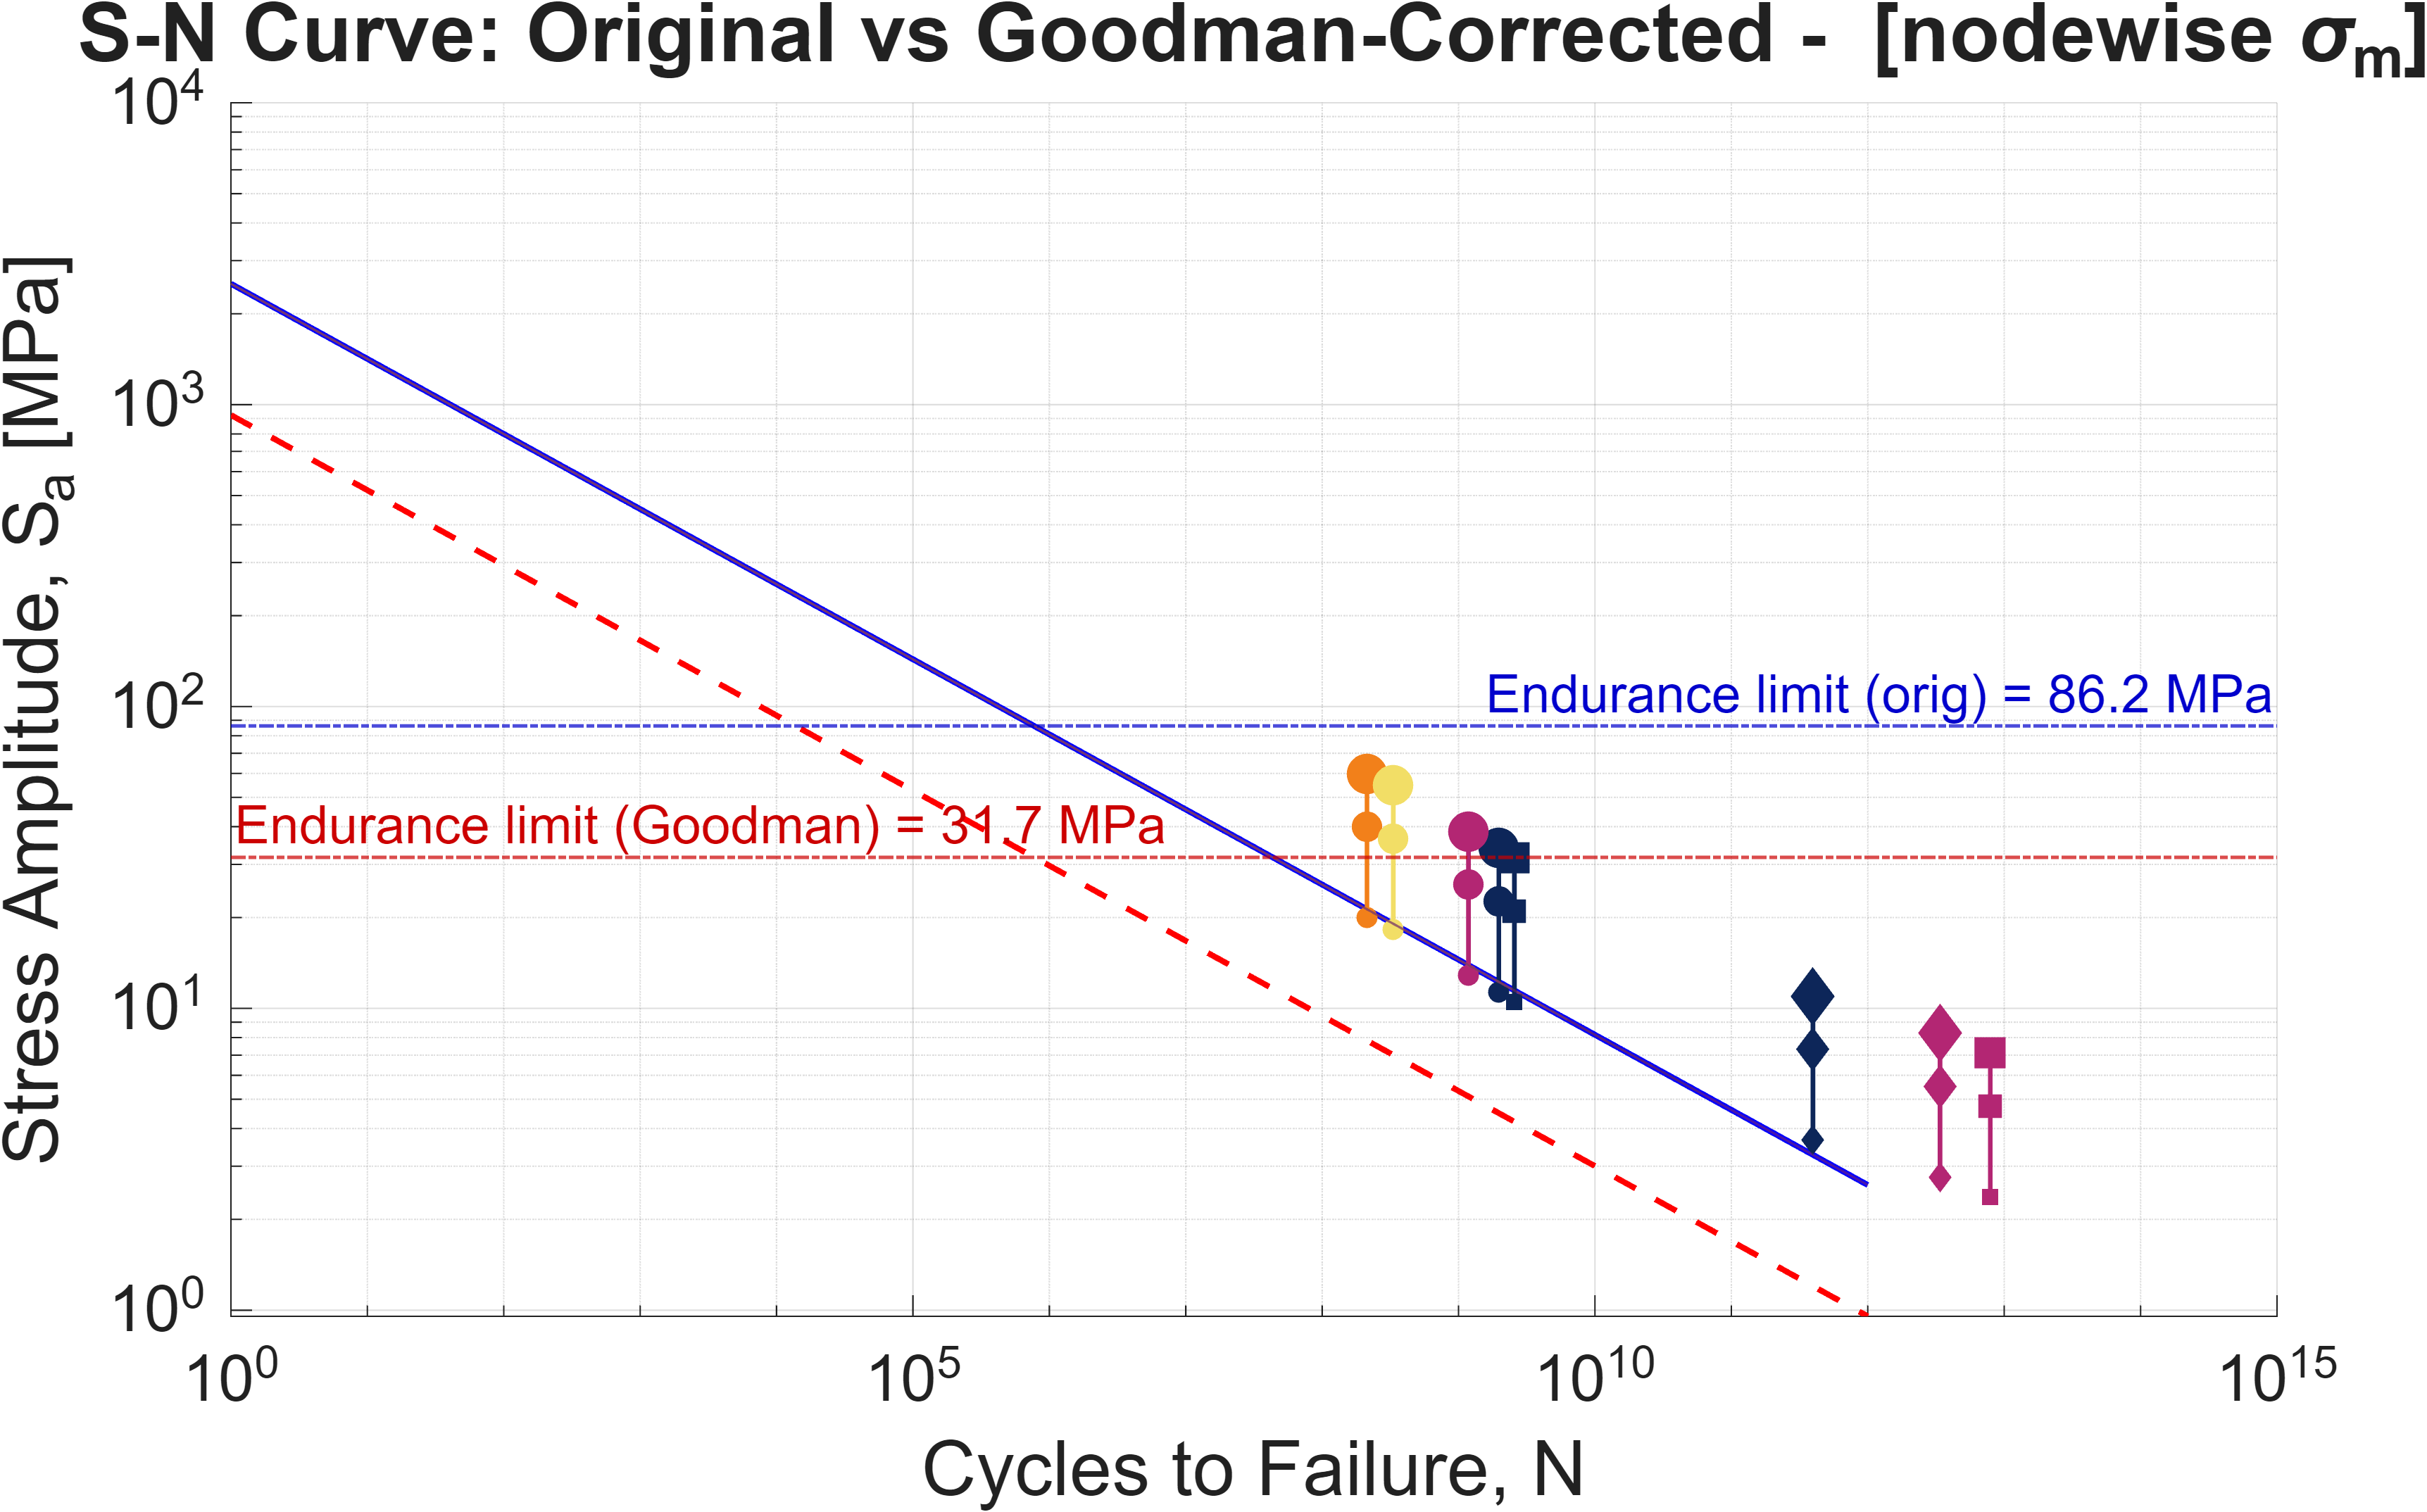
\includegraphics[width=\textwidth]{Axial Nasa/Axial Nasa_sn_curve_goodman_and_rms NODEWISE.png}
        \caption{Axial Loading (bending).}
        \label{fig:NASA_bending_sn_curve_goodman_and_rms_NODEWISE}
    \end{subfigure}
    
    \caption{SN-diagram with nodewise Goodman correction for the NASA Workmanship excitation. (a) Transverse loading.  (b) Axial loading. The same trends are visible in the corresponding T43A results, see Appendix \ref{app:T43A_figures}.}
    \label{fig:SN_NASA}
\end{figure}

For each loading case and finite element model variant (Solid, Beam, Bonded, CBUSH), the most critical node in each stress region is plotted on the SN diagram. The $1\sigma$, $2\sigma$, and $3\sigma$ stress amplitudes are connected by an axial bar. This follows the Steinberg three-band approximation, which is shown as valid in Figures \ref{fig:SteinbergDirlik_members} and \ref{fig:SteinbergDirlik_members_T43A}. The results show that the loading direction is the dominant factor. In the transverse (shear) cases, all critical locations remain below the Goodman-corrected endurance limit even at the $3\sigma$ level, indicating very long or infinite fatigue life.

In the axial (bending) cases, the clamped member stress region becomes critical: the $3\sigma$ amplitudes are approximately 34-60 MPa for the NASA excitation. For the T43A excitation, 3$\sigma$ amplitudes range from 46 MPa (Solid) up to 74 MPa (CBUSH), with the Bonded model reaching approximately 180 MPa, indicating a large stress over-prediction in the bonded representation under broadband axial loading.
The comparison shows that the Goodman mean-stress correction is highly influential, since it shifts several points from the nominally safe region to the unsafe region. Overall, the figures show that an accurate representation of both bolt preload and loading direction is essential for the random-vibration fatigue assessment of bolted joints.

The nominal approach is conservative because it assigns a bolt preload mean stress to every node in the model, including clamped-member nodes far from the bolt that, in reality, carry negligible static stress.

With the nodewise correction (Figures \ref{fig:SN_NASA} and \ref{fig:SN_T43A}), the mean stress applied to each node is the actual static von Mises stress at that location. For the clamped-member nodes, the static preload stress is essentially zero ($\sigma_m < 1$ MPa), yielding $g_f \approx 1$. In the local bolt regions, the static stress can exceed the yield strength, in which case the linear Goodman correction is outside its validity range. The absolute lives plotted there should therefore be read as model-comparison data and not physical predictions.

The consequence is that all nodewise fatigue lives are approximately $g_{f, nom}^{-k} = 0.367^{-4} \approx 56$ times longer than the nominal results. For example, the Solid NASA Axial stress in the clamped members' minimum life increases from $4.79 \times 10^4$ s (nominal) to $2.68 \times 10^6$ s (nodewise), and the pattern is consistent across all load cases. The model ranking and the relative ratios between models remain unchanged.



% DO NOT CHANGE BELOW
\cleardoublepage
\thispagestyle{empty}
\vspace*{\fill}
\clearpage{\thispagestyle{empty}}
\changepage{3cm}{1cm}{-0.5cm}{-0.5cm}{}{-1.5cm}{}{}{}
\vspace*{\fill}
\center

{\bthcsnotextlogo{3cm}}
\\
\noindent\makebox[\linewidth]{\rule{\textwidth}{1pt}} 
Faculty of \faculty, Blekinge Institute of Technology, 371 79 Karlskrona, Sweden
%  -  -  -  -  -  - -

\end{document}